\documentclass[a4paper]{book}
\usepackage{makeidx}
\usepackage{natbib}
\usepackage{graphicx}
\usepackage{multicol}
\usepackage{float}
\usepackage{listings}
\usepackage{color}
\usepackage{ifthen}
\usepackage[table]{xcolor}
\usepackage{textcomp}
\usepackage{alltt}
\usepackage{ifpdf}
\ifpdf
\usepackage[pdftex,
            pagebackref=true,
            colorlinks=true,
            linkcolor=blue,
            unicode
           ]{hyperref}
\else
\usepackage[ps2pdf,
            pagebackref=true,
            colorlinks=true,
            linkcolor=blue,
            unicode
           ]{hyperref}
\usepackage{pspicture}
\fi
\usepackage[utf8]{inputenc}
\usepackage{mathptmx}
\usepackage[scaled=.90]{helvet}
\usepackage{courier}
\usepackage{sectsty}
\usepackage[titles]{tocloft}
\usepackage{doxygen}
\lstset{language=C++,inputencoding=utf8,basicstyle=\footnotesize,breaklines=true,breakatwhitespace=true,tabsize=8,numbers=left }
\makeindex
\setcounter{tocdepth}{3}
\renewcommand{\footrulewidth}{0.4pt}
\renewcommand{\familydefault}{\sfdefault}
\hfuzz=15pt
\setlength{\emergencystretch}{15pt}
\hbadness=750
\tolerance=750
\begin{document}
\hypersetup{pageanchor=false,citecolor=blue}
\begin{titlepage}
\vspace*{7cm}
\begin{center}
{\Large \-General \-Server \\[1ex]\large 1 }\\
\vspace*{1cm}
{\large \-Generated by Doxygen 1.7.6.1}\\
\vspace*{0.5cm}
{\small Thu Apr 30 2015 07:27:14}\\
\end{center}
\end{titlepage}
\clearemptydoublepage
\pagenumbering{roman}
\tableofcontents
\clearemptydoublepage
\pagenumbering{arabic}
\hypersetup{pageanchor=true,citecolor=blue}
\chapter{\-Module \-Index}
\section{\-Modules}
\-Here is a list of all modules\-:\begin{DoxyCompactList}
\item \contentsline{section}{\-X\-S\-L\-Module-\/\-Commands}{\pageref{group__XSLModule-Commands}}{}
\item \contentsline{section}{\-X\-S\-L\-Module-\/\-Functions}{\pageref{group__XSLModule-Functions}}{}
\end{DoxyCompactList}

\chapter{\-Class \-Index}
\section{\-Class \-Hierarchy}
\-This inheritance list is sorted roughly, but not completely, alphabetically\-:\begin{DoxyCompactList}
\item \contentsline{section}{general\-\_\-server\-:\-:\-Access\-Control\-List}{\pageref{classgeneral__server_1_1AccessControlList}}{}
\item \contentsline{section}{general\-\_\-server\-:\-:\-Admin\-Security\-Context}{\pageref{classgeneral__server_1_1AdminSecurityContext}}{}
\item \contentsline{section}{general\-\_\-server\-:\-:\-T\-Xml\-:\-:\-Affected\-Node\-Details}{\pageref{structgeneral__server_1_1TXml_1_1AffectedNodeDetails}}{}
\item \contentsline{section}{general\-\_\-server\-:\-:\-Repository\-:\-:\-Affected\-Repository\-Details}{\pageref{structgeneral__server_1_1Repository_1_1AffectedRepositoryDetails}}{}
\item \contentsline{section}{general\-\_\-server\-:\-:\-Memory\-Lifetime\-Owner\-:\-:\-Allocation}{\pageref{structgeneral__server_1_1MemoryLifetimeOwner_1_1Allocation}}{}
\item \contentsline{section}{general\-\_\-server\-:\-:\-Message\-Interpretation\-:\-:\-Comp}{\pageref{classgeneral__server_1_1MessageInterpretation_1_1Comp}}{}
\item \contentsline{section}{general\-\_\-server\-:\-:\-Database\-Admin\-Query\-Environment}{\pageref{classgeneral__server_1_1DatabaseAdminQueryEnvironment}}{}
\item \contentsline{section}{general\-\_\-server\-:\-:\-Database\-Node}{\pageref{classgeneral__server_1_1DatabaseNode}}{}
\item \contentsline{section}{general\-\_\-server\-:\-:\-Database\-Node\-Server\-Object}{\pageref{classgeneral__server_1_1DatabaseNodeServerObject}}{}
\begin{DoxyCompactList}
\item \contentsline{section}{general\-\_\-server\-:\-:\-General\-Server\-Database\-Node\-Server\-Object}{\pageref{classgeneral__server_1_1GeneralServerDatabaseNodeServerObject}}{}
\begin{DoxyCompactList}
\item \contentsline{section}{general\-\_\-server\-:\-:\-Conversation}{\pageref{classgeneral__server_1_1Conversation}}{}
\item \contentsline{section}{general\-\_\-server\-:\-:\-Database\-Class}{\pageref{classgeneral__server_1_1DatabaseClass}}{}
\item \contentsline{section}{general\-\_\-server\-:\-:\-Message\-Interpretation}{\pageref{classgeneral__server_1_1MessageInterpretation}}{}
\item \contentsline{section}{general\-\_\-server\-:\-:\-Repository}{\pageref{classgeneral__server_1_1Repository}}{}
\begin{DoxyCompactList}
\item \contentsline{section}{general\-\_\-server\-:\-:\-Directory}{\pageref{classgeneral__server_1_1Directory}}{}
\begin{DoxyCompactList}
\item \contentsline{section}{general\-\_\-server\-:\-:\-Resources\-Store}{\pageref{classgeneral__server_1_1ResourcesStore}}{}
\end{DoxyCompactList}
\item \contentsline{section}{general\-\_\-server\-:\-:\-File}{\pageref{classgeneral__server_1_1File}}{}
\begin{DoxyCompactList}
\item \contentsline{section}{general\-\_\-server\-:\-:\-Commit\-File\-Temporary}{\pageref{classgeneral__server_1_1CommitFileTemporary}}{}
\item \contentsline{section}{general\-\_\-server\-:\-:\-Hardlink}{\pageref{classgeneral__server_1_1Hardlink}}{}
\item \contentsline{section}{general\-\_\-server\-:\-:\-Meta\-File}{\pageref{classgeneral__server_1_1MetaFile}}{}
\begin{DoxyCompactList}
\item \contentsline{section}{general\-\_\-server\-:\-:\-Database\-Status\-File}{\pageref{classgeneral__server_1_1DatabaseStatusFile}}{}
\item \contentsline{section}{general\-\_\-server\-:\-:\-Directory\-Details}{\pageref{classgeneral__server_1_1DirectoryDetails}}{}
\item \contentsline{section}{general\-\_\-server\-:\-:\-D\-O\-C\-Type\-Definition}{\pageref{classgeneral__server_1_1DOCTypeDefinition}}{}
\item \contentsline{section}{general\-\_\-server\-:\-:\-Editor\-Backup\-File}{\pageref{classgeneral__server_1_1EditorBackupFile}}{}
\end{DoxyCompactList}
\end{DoxyCompactList}
\item \contentsline{section}{general\-\_\-server\-:\-:\-Internet\-Location}{\pageref{classgeneral__server_1_1InternetLocation}}{}
\item \contentsline{section}{general\-\_\-server\-:\-:\-Relational\-Database}{\pageref{classgeneral__server_1_1RelationalDatabase}}{}
\begin{DoxyCompactList}
\item \contentsline{section}{general\-\_\-server\-:\-:\-My\-S\-Q\-L}{\pageref{classgeneral__server_1_1MySQL}}{}
\item \contentsline{section}{general\-\_\-server\-:\-:\-Postgres}{\pageref{classgeneral__server_1_1Postgres}}{}
\end{DoxyCompactList}
\end{DoxyCompactList}
\item \contentsline{section}{general\-\_\-server\-:\-:\-Request}{\pageref{classgeneral__server_1_1Request}}{}
\item \contentsline{section}{general\-\_\-server\-:\-:\-Server}{\pageref{classgeneral__server_1_1Server}}{}
\item \contentsline{section}{general\-\_\-server\-:\-:\-Service}{\pageref{classgeneral__server_1_1Service}}{}
\item \contentsline{section}{general\-\_\-server\-:\-:\-Session}{\pageref{classgeneral__server_1_1Session}}{}
\item \contentsline{section}{general\-\_\-server\-:\-:\-User}{\pageref{classgeneral__server_1_1User}}{}
\end{DoxyCompactList}
\end{DoxyCompactList}
\item \contentsline{section}{general\-\_\-server\-:\-:\-Debug}{\pageref{classgeneral__server_1_1Debug}}{}
\item \contentsline{section}{delete\-\_\-pointer\-\_\-element$<$ \-T $>$}{\pageref{structdelete__pointer__element}}{}
\item \contentsline{section}{general\-\_\-server\-:\-:\-Exception\-Base}{\pageref{classgeneral__server_1_1ExceptionBase}}{}
\begin{DoxyCompactList}
\item \contentsline{section}{general\-\_\-server\-:\-:\-Attribute\-Required}{\pageref{classgeneral__server_1_1AttributeRequired}}{}
\item \contentsline{section}{general\-\_\-server\-:\-:\-Blank\-Document}{\pageref{classgeneral__server_1_1BlankDocument}}{}
\item \contentsline{section}{general\-\_\-server\-:\-:\-Blank\-Input\-Stream}{\pageref{classgeneral__server_1_1BlankInputStream}}{}
\item \contentsline{section}{general\-\_\-server\-:\-:\-Cannot\-Connect\-Socket}{\pageref{classgeneral__server_1_1CannotConnectSocket}}{}
\item \contentsline{section}{general\-\_\-server\-:\-:\-Cannot\-Convert\-Absolute\-H\-R\-E\-F\-To\-X\-Path\-Without\-Root}{\pageref{classgeneral__server_1_1CannotConvertAbsoluteHREFToXPathWithoutRoot}}{}
\item \contentsline{section}{general\-\_\-server\-:\-:\-Cannot\-Create\-In\-Tmp\-Node}{\pageref{classgeneral__server_1_1CannotCreateInTmpNode}}{}
\item \contentsline{section}{general\-\_\-server\-:\-:\-Cannot\-Create\-Socket}{\pageref{classgeneral__server_1_1CannotCreateSocket}}{}
\item \contentsline{section}{general\-\_\-server\-:\-:\-Cannot\-Reconcile\-Default\-Namespace}{\pageref{classgeneral__server_1_1CannotReconcileDefaultNamespace}}{}
\item \contentsline{section}{general\-\_\-server\-:\-:\-Cannot\-Resolve\-Hostname}{\pageref{classgeneral__server_1_1CannotResolveHostname}}{}
\item \contentsline{section}{general\-\_\-server\-:\-:\-Cannot\-Run\-X\-Path\-Without\-Namespace\-Cache}{\pageref{classgeneral__server_1_1CannotRunXPathWithoutNamespaceCache}}{}
\item \contentsline{section}{general\-\_\-server\-:\-:\-Cannot\-Send\-Data}{\pageref{classgeneral__server_1_1CannotSendData}}{}
\item \contentsline{section}{general\-\_\-server\-:\-:\-Capability\-Not\-Supported}{\pageref{classgeneral__server_1_1CapabilityNotSupported}}{}
\item \contentsline{section}{general\-\_\-server\-:\-:\-C\-D\-A\-T\-A\-End\-Not\-Found}{\pageref{classgeneral__server_1_1CDATAEndNotFound}}{}
\item \contentsline{section}{general\-\_\-server\-:\-:\-Conversation\-Failed\-To\-R\-X\-S\-L\-Input}{\pageref{classgeneral__server_1_1ConversationFailedToRXSLInput}}{}
\item \contentsline{section}{general\-\_\-server\-:\-:\-Database\-Class\-Name\-Required}{\pageref{classgeneral__server_1_1DatabaseClassNameRequired}}{}
\item \contentsline{section}{general\-\_\-server\-:\-:\-Database\-Node\-Server\-Object\-Has\-No\-X\-S\-D\-Name}{\pageref{classgeneral__server_1_1DatabaseNodeServerObjectHasNoXSDName}}{}
\item \contentsline{section}{general\-\_\-server\-:\-:\-Data\-Size\-Abort}{\pageref{classgeneral__server_1_1DataSizeAbort}}{}
\item \contentsline{section}{general\-\_\-server\-:\-:\-Date\-Format\-Result\-Too\-Long}{\pageref{classgeneral__server_1_1DateFormatResultTooLong}}{}
\item \contentsline{section}{general\-\_\-server\-:\-:\-Document\-Mismatch\-For\-Namespace\-Cache\-Copy\-Operation}{\pageref{classgeneral__server_1_1DocumentMismatchForNamespaceCacheCopyOperation}}{}
\item \contentsline{section}{general\-\_\-server\-:\-:\-Document\-Not\-Valid}{\pageref{classgeneral__server_1_1DocumentNotValid}}{}
\item \contentsline{section}{general\-\_\-server\-:\-:\-Document\-Parse\-Error}{\pageref{classgeneral__server_1_1DocumentParseError}}{}
\item \contentsline{section}{general\-\_\-server\-:\-:\-Duplicate\-Database\-Class}{\pageref{classgeneral__server_1_1DuplicateDatabaseClass}}{}
\item \contentsline{section}{general\-\_\-server\-:\-:\-Dynamic\-Path\-To\-Non\-Repository\-Node}{\pageref{classgeneral__server_1_1DynamicPathToNonRepositoryNode}}{}
\item \contentsline{section}{general\-\_\-server\-:\-:\-Exception\-Class\-Not\-Allowed}{\pageref{classgeneral__server_1_1ExceptionClassNotAllowed}}{}
\item \contentsline{section}{general\-\_\-server\-:\-:\-Exception\-Class\-Required}{\pageref{classgeneral__server_1_1ExceptionClassRequired}}{}
\item \contentsline{section}{general\-\_\-server\-:\-:\-Failed\-To\-Compile\-Stylesheet}{\pageref{classgeneral__server_1_1FailedToCompileStylesheet}}{}
\item \contentsline{section}{general\-\_\-server\-:\-:\-Failed\-To\-Open\-Sync\-Directory}{\pageref{classgeneral__server_1_1FailedToOpenSyncDirectory}}{}
\item \contentsline{section}{general\-\_\-server\-:\-:\-Failed\-To\-Parse\-Date}{\pageref{classgeneral__server_1_1FailedToParseDate}}{}
\item \contentsline{section}{general\-\_\-server\-:\-:\-Failed\-To\-Remove\-Old\-Item}{\pageref{classgeneral__server_1_1FailedToRemoveOldItem}}{}
\item \contentsline{section}{general\-\_\-server\-:\-:\-Failed\-To\-Resolve\-X\-S\-L\-Include\-Path}{\pageref{classgeneral__server_1_1FailedToResolveXSLIncludePath}}{}
\item \contentsline{section}{general\-\_\-server\-:\-:\-Failed\-To\-Swap\-In\-Placeholder}{\pageref{classgeneral__server_1_1FailedToSwapInPlaceholder}}{}
\item \contentsline{section}{general\-\_\-server\-:\-:\-File\-Not\-Found}{\pageref{classgeneral__server_1_1FileNotFound}}{}
\item \contentsline{section}{general\-\_\-server\-:\-:\-Hard\-Link\-To\-Nowhere}{\pageref{classgeneral__server_1_1HardLinkToNowhere}}{}
\item \contentsline{section}{general\-\_\-server\-:\-:\-Interface\-Not\-Supported}{\pageref{classgeneral__server_1_1InterfaceNotSupported}}{}
\item \contentsline{section}{general\-\_\-server\-:\-:\-Invalid\-Commit\-Status}{\pageref{classgeneral__server_1_1InvalidCommitStatus}}{}
\item \contentsline{section}{general\-\_\-server\-:\-:\-Invalid\-Commit\-Status\-Name}{\pageref{classgeneral__server_1_1InvalidCommitStatusName}}{}
\item \contentsline{section}{general\-\_\-server\-:\-:\-Invalid\-Commit\-Style}{\pageref{classgeneral__server_1_1InvalidCommitStyle}}{}
\item \contentsline{section}{general\-\_\-server\-:\-:\-Invalid\-Commit\-Style\-Name}{\pageref{classgeneral__server_1_1InvalidCommitStyleName}}{}
\item \contentsline{section}{general\-\_\-server\-:\-:\-Invalid\-Protocol}{\pageref{classgeneral__server_1_1InvalidProtocol}}{}
\item \contentsline{section}{general\-\_\-server\-:\-:\-Invalid\-X\-M\-L}{\pageref{classgeneral__server_1_1InvalidXML}}{}
\item \contentsline{section}{general\-\_\-server\-:\-:\-Invalid\-X\-M\-L\-Name}{\pageref{classgeneral__server_1_1InvalidXMLName}}{}
\item \contentsline{section}{general\-\_\-server\-:\-:\-Login\-Failed}{\pageref{classgeneral__server_1_1LoginFailed}}{}
\item \contentsline{section}{general\-\_\-server\-:\-:\-Memory\-Block\-Not\-Found}{\pageref{classgeneral__server_1_1MemoryBlockNotFound}}{}
\item \contentsline{section}{general\-\_\-server\-:\-:\-Memory\-Blocks\-Un\-Managed}{\pageref{classgeneral__server_1_1MemoryBlocksUnManaged}}{}
\item \contentsline{section}{general\-\_\-server\-:\-:\-Memory\-Children\-Un\-Managed}{\pageref{classgeneral__server_1_1MemoryChildrenUnManaged}}{}
\item \contentsline{section}{general\-\_\-server\-:\-:\-M\-I\-Message\-Transformation\-Required}{\pageref{classgeneral__server_1_1MIMessageTransformationRequired}}{}
\item \contentsline{section}{general\-\_\-server\-:\-:\-M\-I\-Primary\-Output\-Transformation\-Required}{\pageref{classgeneral__server_1_1MIPrimaryOutputTransformationRequired}}{}
\item \contentsline{section}{general\-\_\-server\-:\-:\-Mismatched\-Namespace\-Prefix\-Association}{\pageref{classgeneral__server_1_1MismatchedNamespacePrefixAssociation}}{}
\item \contentsline{section}{general\-\_\-server\-:\-:\-Missing\-Default\-Namespace\-Decleration}{\pageref{classgeneral__server_1_1MissingDefaultNamespaceDecleration}}{}
\item \contentsline{section}{general\-\_\-server\-:\-:\-Missing\-Path\-To\-File}{\pageref{classgeneral__server_1_1MissingPathToFile}}{}
\item \contentsline{section}{general\-\_\-server\-:\-:\-Missing\-Repository\-Name\-Attribute}{\pageref{classgeneral__server_1_1MissingRepositoryNameAttribute}}{}
\item \contentsline{section}{general\-\_\-server\-:\-:\-Multiple\-Resource\-Found}{\pageref{classgeneral__server_1_1MultipleResourceFound}}{}
\item \contentsline{section}{general\-\_\-server\-:\-:\-Multiple\-Root\-Nodes}{\pageref{classgeneral__server_1_1MultipleRootNodes}}{}
\item \contentsline{section}{general\-\_\-server\-:\-:\-Multiple\-Socket\-Errors}{\pageref{classgeneral__server_1_1MultipleSocketErrors}}{}
\item \contentsline{section}{general\-\_\-server\-:\-:\-Namespace\-Is\-Invalid}{\pageref{classgeneral__server_1_1NamespaceIsInvalid}}{}
\item \contentsline{section}{general\-\_\-server\-:\-:\-Native\-Library\-Class\-Required}{\pageref{classgeneral__server_1_1NativeLibraryClassRequired}}{}
\item \contentsline{section}{general\-\_\-server\-:\-:\-No\-Database\-Selected}{\pageref{classgeneral__server_1_1NoDatabaseSelected}}{}
\item \contentsline{section}{general\-\_\-server\-:\-:\-Node\-Addable\-Access\-Denied}{\pageref{classgeneral__server_1_1NodeAddableAccessDenied}}{}
\item \contentsline{section}{general\-\_\-server\-:\-:\-Node\-Writeable\-Access\-Denied}{\pageref{classgeneral__server_1_1NodeWriteableAccessDenied}}{}
\item \contentsline{section}{general\-\_\-server\-:\-:\-No\-Document\-Node\-Found}{\pageref{classgeneral__server_1_1NoDocumentNodeFound}}{}
\item \contentsline{section}{general\-\_\-server\-:\-:\-No\-E\-M\-O\-Available\-For\-Extension}{\pageref{classgeneral__server_1_1NoEMOAvailableForExtension}}{}
\item \contentsline{section}{general\-\_\-server\-:\-:\-No\-Filter\-Target\-Document}{\pageref{classgeneral__server_1_1NoFilterTargetDocument}}{}
\item \contentsline{section}{general\-\_\-server\-:\-:\-Non\-Transient\-Node}{\pageref{classgeneral__server_1_1NonTransientNode}}{}
\item \contentsline{section}{general\-\_\-server\-:\-:\-No\-Ouput\-Document}{\pageref{classgeneral__server_1_1NoOuputDocument}}{}
\item \contentsline{section}{general\-\_\-server\-:\-:\-No\-Output\-Root\-Node}{\pageref{classgeneral__server_1_1NoOutputRootNode}}{}
\item \contentsline{section}{general\-\_\-server\-:\-:\-No\-Root\-Node\-Found}{\pageref{classgeneral__server_1_1NoRootNodeFound}}{}
\item \contentsline{section}{general\-\_\-server\-:\-:\-No\-Servers\-Found\-In\-Main\-Database}{\pageref{classgeneral__server_1_1NoServersFoundInMainDatabase}}{}
\item \contentsline{section}{general\-\_\-server\-:\-:\-No\-Stylesheet}{\pageref{classgeneral__server_1_1NoStylesheet}}{}
\item \contentsline{section}{general\-\_\-server\-:\-:\-No\-Tmp\-Node\-Found}{\pageref{classgeneral__server_1_1NoTmpNodeFound}}{}
\item \contentsline{section}{general\-\_\-server\-:\-:\-Out\-Of\-Memory}{\pageref{classgeneral__server_1_1OutOfMemory}}{}
\item \contentsline{section}{general\-\_\-server\-:\-:\-Pipe\-Failure}{\pageref{classgeneral__server_1_1PipeFailure}}{}
\begin{DoxyCompactList}
\item \contentsline{section}{general\-\_\-server\-:\-:\-Pipe\-Failure\-\_\-\-E\-A\-C\-C\-E\-S}{\pageref{classgeneral__server_1_1PipeFailure__EACCES}}{}
\item \contentsline{section}{general\-\_\-server\-:\-:\-Pipe\-Failure\-\_\-\-E\-P\-I\-P\-E}{\pageref{classgeneral__server_1_1PipeFailure__EPIPE}}{}
\item \contentsline{section}{general\-\_\-server\-:\-:\-Pipe\-Failure\-\_\-\-Generic}{\pageref{classgeneral__server_1_1PipeFailure__Generic}}{}
\end{DoxyCompactList}
\item \contentsline{section}{general\-\_\-server\-:\-:\-Protocol\-Not\-Supported}{\pageref{classgeneral__server_1_1ProtocolNotSupported}}{}
\item \contentsline{section}{general\-\_\-server\-:\-:\-Relational\-Database\-Connection\-Failed}{\pageref{classgeneral__server_1_1RelationalDatabaseConnectionFailed}}{}
\item \contentsline{section}{general\-\_\-server\-:\-:\-Replace\-Node\-Requires\-Constant\-X\-M\-L\-I\-D}{\pageref{classgeneral__server_1_1ReplaceNodeRequiresConstantXMLID}}{}
\item \contentsline{section}{general\-\_\-server\-:\-:\-Repository\-Type\-Missing}{\pageref{classgeneral__server_1_1RepositoryTypeMissing}}{}
\item \contentsline{section}{general\-\_\-server\-:\-:\-Repository\-Type\-Unknown}{\pageref{classgeneral__server_1_1RepositoryTypeUnknown}}{}
\item \contentsline{section}{general\-\_\-server\-:\-:\-Resource\-Not\-Found}{\pageref{classgeneral__server_1_1ResourceNotFound}}{}
\item \contentsline{section}{general\-\_\-server\-:\-:\-Resources\-Copy\-Failure}{\pageref{classgeneral__server_1_1ResourcesCopyFailure}}{}
\item \contentsline{section}{general\-\_\-server\-:\-:\-Response\-Tag\-Malformed}{\pageref{classgeneral__server_1_1ResponseTagMalformed}}{}
\item \contentsline{section}{general\-\_\-server\-:\-:\-Semaphore\-Failure}{\pageref{classgeneral__server_1_1SemaphoreFailure}}{}
\item \contentsline{section}{general\-\_\-server\-:\-:\-Service\-Cannot\-Listen}{\pageref{classgeneral__server_1_1ServiceCannotListen}}{}
\item \contentsline{section}{general\-\_\-server\-:\-:\-Service\-M\-Is\-Required}{\pageref{classgeneral__server_1_1ServiceMIsRequired}}{}
\item \contentsline{section}{general\-\_\-server\-:\-:\-Service\-Port\-Required}{\pageref{classgeneral__server_1_1ServicePortRequired}}{}
\item \contentsline{section}{general\-\_\-server\-:\-:\-Session\-Required}{\pageref{classgeneral__server_1_1SessionRequired}}{}
\item \contentsline{section}{general\-\_\-server\-:\-:\-Standard\-Exception}{\pageref{classgeneral__server_1_1StandardException}}{}
\item \contentsline{section}{general\-\_\-server\-:\-:\-Sub\-Repository\-Not\-Found\-For\-Node}{\pageref{classgeneral__server_1_1SubRepositoryNotFoundForNode}}{}
\item \contentsline{section}{general\-\_\-server\-:\-:\-Thread\-Type\-Unknown}{\pageref{classgeneral__server_1_1ThreadTypeUnknown}}{}
\item \contentsline{section}{general\-\_\-server\-:\-:\-Transform\-Failed}{\pageref{classgeneral__server_1_1TransformFailed}}{}
\item \contentsline{section}{general\-\_\-server\-:\-:\-Transform\-Without\-Current\-Node}{\pageref{classgeneral__server_1_1TransformWithoutCurrentNode}}{}
\item \contentsline{section}{general\-\_\-server\-:\-:\-Transient\-Node}{\pageref{classgeneral__server_1_1TransientNode}}{}
\item \contentsline{section}{general\-\_\-server\-:\-:\-T\-Xml\-Application\-Failed}{\pageref{classgeneral__server_1_1TXmlApplicationFailed}}{}
\item \contentsline{section}{general\-\_\-server\-:\-:\-T\-Xml\-Cannot\-Open\-Transaction\-Store}{\pageref{classgeneral__server_1_1TXmlCannotOpenTransactionStore}}{}
\item \contentsline{section}{general\-\_\-server\-:\-:\-T\-Xml\-Failed\-To\-Parse\-Transaction\-X\-M\-L}{\pageref{classgeneral__server_1_1TXmlFailedToParseTransactionXML}}{}
\item \contentsline{section}{general\-\_\-server\-:\-:\-T\-Xml\-Invalid}{\pageref{classgeneral__server_1_1TXmlInvalid}}{}
\item \contentsline{section}{general\-\_\-server\-:\-:\-T\-Xml\-Required\-Node\-Not\-Found}{\pageref{classgeneral__server_1_1TXmlRequiredNodeNotFound}}{}
\item \contentsline{section}{general\-\_\-server\-:\-:\-T\-Xml\-Serialisation\-Parent\-Null}{\pageref{classgeneral__server_1_1TXmlSerialisationParentNull}}{}
\item \contentsline{section}{general\-\_\-server\-:\-:\-T\-Xml\-Transform\-Not\-Supported\-For}{\pageref{classgeneral__server_1_1TXmlTransformNotSupportedFor}}{}
\item \contentsline{section}{general\-\_\-server\-:\-:\-T\-Xml\-Unknown\-Transaction\-Type}{\pageref{classgeneral__server_1_1TXmlUnknownTransactionType}}{}
\item \contentsline{section}{general\-\_\-server\-:\-:\-T\-Xml\-Volatile\-Result}{\pageref{classgeneral__server_1_1TXmlVolatileResult}}{}
\item \contentsline{section}{general\-\_\-server\-:\-:\-Unknown\-File\-Type}{\pageref{classgeneral__server_1_1UnknownFileType}}{}
\item \contentsline{section}{general\-\_\-server\-:\-:\-Unknown\-Hardlink\-Policy}{\pageref{classgeneral__server_1_1UnknownHardlinkPolicy}}{}
\item \contentsline{section}{general\-\_\-server\-:\-:\-Unkown\-Security\-Strategy\-Name}{\pageref{classgeneral__server_1_1UnkownSecurityStrategyName}}{}
\item \contentsline{section}{general\-\_\-server\-:\-:\-Unregistered\-Database\-Class}{\pageref{classgeneral__server_1_1UnregisteredDatabaseClass}}{}
\item \contentsline{section}{general\-\_\-server\-:\-:\-Un\-Winder}{\pageref{classgeneral__server_1_1UnWinder}}{}
\item \contentsline{section}{general\-\_\-server\-:\-:\-Up}{\pageref{classgeneral__server_1_1Up}}{}
\item \contentsline{section}{general\-\_\-server\-:\-:\-User\-Does\-Not\-Have\-Permission}{\pageref{classgeneral__server_1_1UserDoesNotHavePermission}}{}
\item \contentsline{section}{general\-\_\-server\-:\-:\-Validity\-Check\-Failure}{\pageref{classgeneral__server_1_1ValidityCheckFailure}}{}
\item \contentsline{section}{general\-\_\-server\-:\-:\-Wrong\-Issuer\-Security\-Context}{\pageref{classgeneral__server_1_1WrongIssuerSecurityContext}}{}
\item \contentsline{section}{general\-\_\-server\-:\-:\-Xml\-Generic\-Exception}{\pageref{classgeneral__server_1_1XmlGenericException}}{}
\item \contentsline{section}{general\-\_\-server\-:\-:\-X\-M\-L\-I\-D\-\_\-\-Duplication\-Issue}{\pageref{classgeneral__server_1_1XMLID__DuplicationIssue}}{}
\item \contentsline{section}{general\-\_\-server\-:\-:\-Xml\-Id\-Redefined}{\pageref{classgeneral__server_1_1XmlIdRedefined}}{}
\item \contentsline{section}{general\-\_\-server\-:\-:\-X\-M\-L\-Parse\-Failed\-At}{\pageref{classgeneral__server_1_1XMLParseFailedAt}}{}
\item \contentsline{section}{general\-\_\-server\-:\-:\-Xml\-Parser\-Namespace\-Not\-Declared}{\pageref{classgeneral__server_1_1XmlParserNamespaceNotDeclared}}{}
\item \contentsline{section}{general\-\_\-server\-:\-:\-X\-Path\-Exception}{\pageref{classgeneral__server_1_1XPathException}}{}
\item \contentsline{section}{general\-\_\-server\-:\-:\-X\-Path\-Function\-Wrong\-Argument\-Type}{\pageref{classgeneral__server_1_1XPathFunctionWrongArgumentType}}{}
\item \contentsline{section}{general\-\_\-server\-:\-:\-X\-Path\-Multiple\-Nodes}{\pageref{classgeneral__server_1_1XPathMultipleNodes}}{}
\item \contentsline{section}{general\-\_\-server\-:\-:\-X\-Path\-Returned\-Empty\-Result\-Set}{\pageref{classgeneral__server_1_1XPathReturnedEmptyResultSet}}{}
\item \contentsline{section}{general\-\_\-server\-:\-:\-X\-Path\-String\-Argument\-Required}{\pageref{classgeneral__server_1_1XPathStringArgumentRequired}}{}
\item \contentsline{section}{general\-\_\-server\-:\-:\-X\-Path\-Type\-Unhandled}{\pageref{classgeneral__server_1_1XPathTypeUnhandled}}{}
\item \contentsline{section}{general\-\_\-server\-:\-:\-X\-S\-L\-Element\-Exception}{\pageref{classgeneral__server_1_1XSLElementException}}{}
\item \contentsline{section}{general\-\_\-server\-:\-:\-X\-S\-L\-Stylesheet\-Node\-Not\-Found}{\pageref{classgeneral__server_1_1XSLStylesheetNodeNotFound}}{}
\item \contentsline{section}{general\-\_\-server\-:\-:\-X\-S\-L\-T\-Exception}{\pageref{classgeneral__server_1_1XSLTException}}{}
\item \contentsline{section}{general\-\_\-server\-:\-:\-X\-S\-L\-T\-Extension\-Not\-Found}{\pageref{classgeneral__server_1_1XSLTExtensionNotFound}}{}
\item \contentsline{section}{general\-\_\-server\-:\-:\-Zero\-Document}{\pageref{classgeneral__server_1_1ZeroDocument}}{}
\item \contentsline{section}{general\-\_\-server\-:\-:\-Zero\-Input\-Stream}{\pageref{classgeneral__server_1_1ZeroInputStream}}{}
\end{DoxyCompactList}
\item \contentsline{section}{general\-\_\-server\-:\-:\-E\-X\-S\-L\-T\-Reg\-Exp}{\pageref{classgeneral__server_1_1EXSLTRegExp}}{}
\item \contentsline{section}{general\-\_\-server\-:\-:\-E\-X\-S\-L\-T\-Strings}{\pageref{classgeneral__server_1_1EXSLTStrings}}{}
\item \contentsline{section}{general\-\_\-server\-:\-:\-Message\-Interpretation\-:\-:\-Gimme\-Pred}{\pageref{classgeneral__server_1_1MessageInterpretation_1_1GimmePred}}{}
\item \contentsline{section}{implements\-\_\-interface \-I\-Xml\-Node\-List}{\pageref{classimplements__interface_01IXmlNodeList}}{}
\begin{DoxyCompactList}
\item \contentsline{section}{general\-\_\-server\-:\-:\-Xml\-Node\-List$<$ \-I\-Xml\-Node\-Type $>$}{\pageref{classgeneral__server_1_1XmlNodeList}}{}
\end{DoxyCompactList}
\item \contentsline{section}{general\-\_\-server\-:\-:\-I\-O\-File}{\pageref{classgeneral__server_1_1IOFile}}{}
\begin{DoxyCompactList}
\item \contentsline{section}{general\-\_\-server\-:\-:\-File}{\pageref{classgeneral__server_1_1File}}{}
\item \contentsline{section}{general\-\_\-server\-:\-:\-I\-O\-Directory}{\pageref{classgeneral__server_1_1IODirectory}}{}
\begin{DoxyCompactList}
\item \contentsline{section}{general\-\_\-server\-:\-:\-Directory}{\pageref{classgeneral__server_1_1Directory}}{}
\end{DoxyCompactList}
\end{DoxyCompactList}
\item \contentsline{section}{general\-\_\-server\-:\-:\-Less\-Fctr}{\pageref{classgeneral__server_1_1LessFctr}}{}
\item \contentsline{section}{general\-\_\-server\-:\-:\-Lib\-Xml\-Area}{\pageref{classgeneral__server_1_1LibXmlArea}}{}
\item \contentsline{section}{general\-\_\-server\-:\-:\-Lib\-Xml\-Node\-Mask}{\pageref{classgeneral__server_1_1LibXmlNodeMask}}{}
\item \contentsline{section}{general\-\_\-server\-:\-:\-Lib\-Xsl\-Module}{\pageref{classgeneral__server_1_1LibXslModule}}{}
\item \contentsline{section}{map}{\pageref{classmap}}{}
\begin{DoxyCompactList}
\item \contentsline{section}{general\-\_\-server\-:\-:\-String\-Map$<$ \-T, \-C $>$}{\pageref{classgeneral__server_1_1StringMap}}{}
\item \contentsline{section}{general\-\_\-server\-:\-:\-Xml\-Node\-Map$<$ \-T $>$}{\pageref{classgeneral__server_1_1XmlNodeMap}}{}
\end{DoxyCompactList}
\item \contentsline{section}{general\-\_\-server\-:\-:\-Memory\-Lifetime\-Owner}{\pageref{classgeneral__server_1_1MemoryLifetimeOwner}}{}
\begin{DoxyCompactList}
\item \contentsline{section}{general\-\_\-server\-:\-:\-Database}{\pageref{classgeneral__server_1_1Database}}{}
\item \contentsline{section}{general\-\_\-server\-:\-:\-Main}{\pageref{classgeneral__server_1_1Main}}{}
\item \contentsline{section}{general\-\_\-server\-:\-:\-Profiler\-Thread}{\pageref{classgeneral__server_1_1ProfilerThread}}{}
\begin{DoxyCompactList}
\item \contentsline{section}{general\-\_\-server\-:\-:\-Conversation}{\pageref{classgeneral__server_1_1Conversation}}{}
\end{DoxyCompactList}
\item \contentsline{section}{general\-\_\-server\-:\-:\-Request}{\pageref{classgeneral__server_1_1Request}}{}
\item \contentsline{section}{general\-\_\-server\-:\-:\-Server}{\pageref{classgeneral__server_1_1Server}}{}
\item \contentsline{section}{general\-\_\-server\-:\-:\-Service}{\pageref{classgeneral__server_1_1Service}}{}
\end{DoxyCompactList}
\item \contentsline{section}{general\-\_\-server\-:\-:\-Query\-Environment}{\pageref{classgeneral__server_1_1QueryEnvironment}}{}
\begin{DoxyCompactList}
\item \contentsline{section}{general\-\_\-server\-:\-:\-Browser\-Query\-Environment}{\pageref{classgeneral__server_1_1BrowserQueryEnvironment}}{}
\end{DoxyCompactList}
\item \contentsline{section}{general\-\_\-server\-:\-:\-Repository\-Save\-Security\-Context}{\pageref{classgeneral__server_1_1RepositorySaveSecurityContext}}{}
\item \contentsline{section}{general\-\_\-server\-:\-:\-Response}{\pageref{classgeneral__server_1_1Response}}{}
\item \contentsline{section}{general\-\_\-server\-:\-:\-Rxsl}{\pageref{classgeneral__server_1_1Rxsl}}{}
\item \contentsline{section}{general\-\_\-server\-:\-:\-Security\-Context}{\pageref{classgeneral__server_1_1SecurityContext}}{}
\begin{DoxyCompactList}
\item \contentsline{section}{general\-\_\-server\-:\-:\-Database\-Node\-User\-Store\-Security\-Context}{\pageref{classgeneral__server_1_1DatabaseNodeUserStoreSecurityContext}}{}
\end{DoxyCompactList}
\item \contentsline{section}{general\-\_\-server\-:\-:\-Repository\-:\-:\-Streaming\-Context}{\pageref{classgeneral__server_1_1Repository_1_1StreamingContext}}{}
\item \contentsline{section}{general\-\_\-server\-:\-:\-String\-Multi\-Map$<$ \-T, \-C $>$}{\pageref{classgeneral__server_1_1StringMultiMap}}{}
\item \contentsline{section}{general\-\_\-server\-:\-:\-Thread\-Caller}{\pageref{classgeneral__server_1_1ThreadCaller}}{}
\begin{DoxyCompactList}
\item \contentsline{section}{general\-\_\-server\-:\-:\-Server}{\pageref{classgeneral__server_1_1Server}}{}
\item \contentsline{section}{general\-\_\-server\-:\-:\-Thread}{\pageref{classgeneral__server_1_1Thread}}{}
\begin{DoxyCompactList}
\item \contentsline{section}{general\-\_\-server\-:\-:\-Command\-Line\-Processor}{\pageref{classgeneral__server_1_1CommandLineProcessor}}{}
\item \contentsline{section}{general\-\_\-server\-:\-:\-Profile\-Monitor}{\pageref{classgeneral__server_1_1ProfileMonitor}}{}
\item \contentsline{section}{general\-\_\-server\-:\-:\-Profiler\-Thread}{\pageref{classgeneral__server_1_1ProfilerThread}}{}
\item \contentsline{section}{general\-\_\-server\-:\-:\-Service}{\pageref{classgeneral__server_1_1Service}}{}
\end{DoxyCompactList}
\end{DoxyCompactList}
\item \contentsline{section}{general\-\_\-server\-:\-:\-Trigger\-Context\-Database\-Attribute}{\pageref{classgeneral__server_1_1TriggerContextDatabaseAttribute}}{}
\item \contentsline{section}{general\-\_\-server\-:\-:\-T\-Xml}{\pageref{classgeneral__server_1_1TXml}}{}
\begin{DoxyCompactList}
\item \contentsline{section}{general\-\_\-server\-:\-:\-T\-Xml\-\_\-\-Change\-Name}{\pageref{classgeneral__server_1_1TXml__ChangeName}}{}
\item \contentsline{section}{general\-\_\-server\-:\-:\-T\-Xml\-\_\-\-Copy\-Child}{\pageref{classgeneral__server_1_1TXml__CopyChild}}{}
\item \contentsline{section}{general\-\_\-server\-:\-:\-T\-Xml\-\_\-\-Create\-Child\-Element}{\pageref{classgeneral__server_1_1TXml__CreateChildElement}}{}
\item \contentsline{section}{general\-\_\-server\-:\-:\-T\-Xml\-\_\-\-Hardlink\-Child}{\pageref{classgeneral__server_1_1TXml__HardlinkChild}}{}
\item \contentsline{section}{general\-\_\-server\-:\-:\-T\-Xml\-\_\-\-Move\-Child}{\pageref{classgeneral__server_1_1TXml__MoveChild}}{}
\item \contentsline{section}{general\-\_\-server\-:\-:\-T\-Xml\-\_\-\-Remove\-Node}{\pageref{classgeneral__server_1_1TXml__RemoveNode}}{}
\item \contentsline{section}{general\-\_\-server\-:\-:\-T\-Xml\-\_\-\-Replace\-Node}{\pageref{classgeneral__server_1_1TXml__ReplaceNode}}{}
\item \contentsline{section}{general\-\_\-server\-:\-:\-T\-Xml\-\_\-\-Set\-Attribute}{\pageref{classgeneral__server_1_1TXml__SetAttribute}}{}
\item \contentsline{section}{general\-\_\-server\-:\-:\-T\-Xml\-\_\-\-Set\-Value}{\pageref{classgeneral__server_1_1TXml__SetValue}}{}
\item \contentsline{section}{general\-\_\-server\-:\-:\-T\-Xml\-\_\-\-Softlink\-Child}{\pageref{classgeneral__server_1_1TXml__SoftlinkChild}}{}
\item \contentsline{section}{general\-\_\-server\-:\-:\-T\-Xml\-\_\-\-Touch\-Node}{\pageref{classgeneral__server_1_1TXml__TouchNode}}{}
\end{DoxyCompactList}
\item \contentsline{section}{general\-\_\-server\-:\-:\-T\-Xml\-Processor}{\pageref{classgeneral__server_1_1TXmlProcessor}}{}
\begin{DoxyCompactList}
\item \contentsline{section}{general\-\_\-server\-:\-:\-Database}{\pageref{classgeneral__server_1_1Database}}{}
\item \contentsline{section}{general\-\_\-server\-:\-:\-Repository}{\pageref{classgeneral__server_1_1Repository}}{}
\end{DoxyCompactList}
\item \contentsline{section}{general\-\_\-server\-:\-:\-Unix\-Security\-Strategy}{\pageref{classgeneral__server_1_1UnixSecurityStrategy}}{}
\item \contentsline{section}{vector}{\pageref{classvector}}{}
\begin{DoxyCompactList}
\item \contentsline{section}{general\-\_\-server\-:\-:\-Mask\-Context}{\pageref{classgeneral__server_1_1MaskContext}}{}
\item \contentsline{section}{general\-\_\-server\-:\-:\-Repository}{\pageref{classgeneral__server_1_1Repository}}{}
\item \contentsline{section}{general\-\_\-server\-:\-:\-String\-Vector}{\pageref{classgeneral__server_1_1StringVector}}{}
\item \contentsline{section}{general\-\_\-server\-:\-:\-T\-Xml\-Collection}{\pageref{classgeneral__server_1_1TXmlCollection}}{}
\item \contentsline{section}{general\-\_\-server\-:\-:\-Xml\-Node\-List$<$ \-I\-Xml\-Node\-Type $>$}{\pageref{classgeneral__server_1_1XmlNodeList}}{}
\end{DoxyCompactList}
\item \contentsline{section}{\-Virtual\-Pointer\-Wrapper\-Class$<$ \-Item $>$}{\pageref{classVirtualPointerWrapperClass}}{}
\item \contentsline{section}{\-Virtual\-Pointer\-Wrapper\-Class\-Checker}{\pageref{classVirtualPointerWrapperClassChecker}}{}
\item \contentsline{section}{\-Virtual\-Pointer\-Wrapper\-Class\-Confirmation}{\pageref{classVirtualPointerWrapperClassConfirmation}}{}
\item \contentsline{section}{\-Virtual\-Pointer\-Wrapper\-Class\-Has\-Members}{\pageref{classVirtualPointerWrapperClassHasMembers}}{}
\item \contentsline{section}{general\-\_\-server\-:\-:\-Xml\-Admin\-Query\-Environment}{\pageref{classgeneral__server_1_1XmlAdminQueryEnvironment}}{}
\item \contentsline{section}{general\-\_\-server\-:\-:\-Xml\-Base\-Doc}{\pageref{classgeneral__server_1_1XmlBaseDoc}}{}
\begin{DoxyCompactList}
\item \contentsline{section}{general\-\_\-server\-:\-:\-Lib\-Xml\-Base\-Doc}{\pageref{classgeneral__server_1_1LibXmlBaseDoc}}{}
\begin{DoxyCompactList}
\item \contentsline{section}{general\-\_\-server\-:\-:\-Lib\-Xml\-Doc}{\pageref{classgeneral__server_1_1LibXmlDoc}}{}
\item \contentsline{section}{general\-\_\-server\-:\-:\-Lib\-Xsl\-Doc}{\pageref{classgeneral__server_1_1LibXslDoc}}{}
\end{DoxyCompactList}
\end{DoxyCompactList}
\item \contentsline{section}{general\-\_\-server\-:\-:\-Xml\-Doc}{\pageref{classgeneral__server_1_1XmlDoc}}{}
\begin{DoxyCompactList}
\item \contentsline{section}{general\-\_\-server\-:\-:\-Lib\-Xml\-Doc}{\pageref{classgeneral__server_1_1LibXmlDoc}}{}
\end{DoxyCompactList}
\item \contentsline{section}{general\-\_\-server\-:\-:\-Xml\-Has\-Namespace\-Definitions}{\pageref{classgeneral__server_1_1XmlHasNamespaceDefinitions}}{}
\begin{DoxyCompactList}
\item \contentsline{section}{general\-\_\-server\-:\-:\-Xml\-Base\-Node}{\pageref{classgeneral__server_1_1XmlBaseNode}}{}
\begin{DoxyCompactList}
\item \contentsline{section}{general\-\_\-server\-:\-:\-Lib\-Xml\-Base\-Node}{\pageref{classgeneral__server_1_1LibXmlBaseNode}}{}
\begin{DoxyCompactList}
\item \contentsline{section}{general\-\_\-server\-:\-:\-Lib\-Xml\-Node}{\pageref{classgeneral__server_1_1LibXmlNode}}{}
\item \contentsline{section}{general\-\_\-server\-:\-:\-Lib\-Xsl\-Command\-Node}{\pageref{classgeneral__server_1_1LibXslCommandNode}}{}
\begin{DoxyCompactList}
\item \contentsline{section}{general\-\_\-server\-:\-:\-Lib\-Xsl\-Node}{\pageref{classgeneral__server_1_1LibXslNode}}{}
\begin{DoxyCompactList}
\item \contentsline{section}{general\-\_\-server\-:\-:\-Lib\-Xsl\-Stylesheet\-Node}{\pageref{classgeneral__server_1_1LibXslStylesheetNode}}{}
\end{DoxyCompactList}
\end{DoxyCompactList}
\end{DoxyCompactList}
\end{DoxyCompactList}
\end{DoxyCompactList}
\item \contentsline{section}{general\-\_\-server\-:\-:\-Xml\-Library}{\pageref{classgeneral__server_1_1XmlLibrary}}{}
\begin{DoxyCompactList}
\item \contentsline{section}{general\-\_\-server\-:\-:\-Lib\-Xml\-Library}{\pageref{classgeneral__server_1_1LibXmlLibrary}}{}
\end{DoxyCompactList}
\item \contentsline{section}{general\-\_\-server\-:\-:\-Xml\-Namespaced}{\pageref{classgeneral__server_1_1XmlNamespaced}}{}
\begin{DoxyCompactList}
\item \contentsline{section}{general\-\_\-server\-:\-:\-Xml\-Base\-Node}{\pageref{classgeneral__server_1_1XmlBaseNode}}{}
\end{DoxyCompactList}
\item \contentsline{section}{general\-\_\-server\-:\-:\-Xml\-Node}{\pageref{classgeneral__server_1_1XmlNode}}{}
\begin{DoxyCompactList}
\item \contentsline{section}{general\-\_\-server\-:\-:\-Lib\-Xml\-Node}{\pageref{classgeneral__server_1_1LibXmlNode}}{}
\end{DoxyCompactList}
\item \contentsline{section}{general\-\_\-server\-:\-:\-Xsl\-Command\-Node}{\pageref{classgeneral__server_1_1XslCommandNode}}{}
\begin{DoxyCompactList}
\item \contentsline{section}{general\-\_\-server\-:\-:\-Lib\-Xsl\-Command\-Node}{\pageref{classgeneral__server_1_1LibXslCommandNode}}{}
\end{DoxyCompactList}
\item \contentsline{section}{general\-\_\-server\-:\-:\-Xsl\-Doc}{\pageref{classgeneral__server_1_1XslDoc}}{}
\begin{DoxyCompactList}
\item \contentsline{section}{general\-\_\-server\-:\-:\-Lib\-Xsl\-Doc}{\pageref{classgeneral__server_1_1LibXslDoc}}{}
\end{DoxyCompactList}
\item \contentsline{section}{general\-\_\-server\-:\-:\-Xsl\-Module}{\pageref{classgeneral__server_1_1XslModule}}{}
\item \contentsline{section}{general\-\_\-server\-:\-:\-Xsl\-Module\-Manager}{\pageref{classgeneral__server_1_1XslModuleManager}}{}
\begin{DoxyCompactList}
\item \contentsline{section}{general\-\_\-server\-:\-:\-Conversation}{\pageref{classgeneral__server_1_1Conversation}}{}
\item \contentsline{section}{general\-\_\-server\-:\-:\-Database}{\pageref{classgeneral__server_1_1Database}}{}
\item \contentsline{section}{general\-\_\-server\-:\-:\-Request}{\pageref{classgeneral__server_1_1Request}}{}
\end{DoxyCompactList}
\item \contentsline{section}{general\-\_\-server\-:\-:\-Xsl\-Node}{\pageref{classgeneral__server_1_1XslNode}}{}
\begin{DoxyCompactList}
\item \contentsline{section}{general\-\_\-server\-:\-:\-Lib\-Xsl\-Node}{\pageref{classgeneral__server_1_1LibXslNode}}{}
\end{DoxyCompactList}
\item \contentsline{section}{general\-\_\-server\-:\-:\-Xsl\-Stylesheet\-Node}{\pageref{classgeneral__server_1_1XslStylesheetNode}}{}
\begin{DoxyCompactList}
\item \contentsline{section}{general\-\_\-server\-:\-:\-Lib\-Xsl\-Stylesheet\-Node}{\pageref{classgeneral__server_1_1LibXslStylesheetNode}}{}
\end{DoxyCompactList}
\item \contentsline{section}{general\-\_\-server\-:\-:\-X\-S\-L\-T\-Custom\-Utilities}{\pageref{classgeneral__server_1_1XSLTCustomUtilities}}{}
\item \contentsline{section}{general\-\_\-server\-:\-:\-Xsl\-Transform\-Context}{\pageref{classgeneral__server_1_1XslTransformContext}}{}
\begin{DoxyCompactList}
\item \contentsline{section}{general\-\_\-server\-:\-:\-Lib\-Xsl\-Transform\-Context}{\pageref{classgeneral__server_1_1LibXslTransformContext}}{}
\end{DoxyCompactList}
\item \contentsline{section}{general\-\_\-server\-:\-:\-Xsl\-X\-Path\-Function\-Context}{\pageref{classgeneral__server_1_1XslXPathFunctionContext}}{}
\begin{DoxyCompactList}
\item \contentsline{section}{general\-\_\-server\-:\-:\-Lib\-Xsl\-X\-Path\-Function\-Context}{\pageref{classgeneral__server_1_1LibXslXPathFunctionContext}}{}
\end{DoxyCompactList}
\end{DoxyCompactList}

\chapter{\-Class \-Index}
\section{\-Class \-List}
\-Here are the classes, structs, unions and interfaces with brief descriptions\-:\begin{DoxyCompactList}
\item\contentsline{section}{\hyperlink{classgeneral__server_1_1AccessControlList}{general\-\_\-server\-::\-Access\-Control\-List} }{\pageref{classgeneral__server_1_1AccessControlList}}{}
\item\contentsline{section}{\hyperlink{classgeneral__server_1_1AdminSecurityContext}{general\-\_\-server\-::\-Admin\-Security\-Context} }{\pageref{classgeneral__server_1_1AdminSecurityContext}}{}
\item\contentsline{section}{\hyperlink{structgeneral__server_1_1TXml_1_1AffectedNodeDetails}{general\-\_\-server\-::\-T\-Xml\-::\-Affected\-Node\-Details} }{\pageref{structgeneral__server_1_1TXml_1_1AffectedNodeDetails}}{}
\item\contentsline{section}{\hyperlink{structgeneral__server_1_1Repository_1_1AffectedRepositoryDetails}{general\-\_\-server\-::\-Repository\-::\-Affected\-Repository\-Details} }{\pageref{structgeneral__server_1_1Repository_1_1AffectedRepositoryDetails}}{}
\item\contentsline{section}{\hyperlink{structgeneral__server_1_1MemoryLifetimeOwner_1_1Allocation}{general\-\_\-server\-::\-Memory\-Lifetime\-Owner\-::\-Allocation} }{\pageref{structgeneral__server_1_1MemoryLifetimeOwner_1_1Allocation}}{}
\item\contentsline{section}{\hyperlink{classgeneral__server_1_1AttributeRequired}{general\-\_\-server\-::\-Attribute\-Required} }{\pageref{classgeneral__server_1_1AttributeRequired}}{}
\item\contentsline{section}{\hyperlink{classgeneral__server_1_1BlankDocument}{general\-\_\-server\-::\-Blank\-Document} }{\pageref{classgeneral__server_1_1BlankDocument}}{}
\item\contentsline{section}{\hyperlink{classgeneral__server_1_1BlankInputStream}{general\-\_\-server\-::\-Blank\-Input\-Stream} }{\pageref{classgeneral__server_1_1BlankInputStream}}{}
\item\contentsline{section}{\hyperlink{classgeneral__server_1_1BrowserQueryEnvironment}{general\-\_\-server\-::\-Browser\-Query\-Environment} }{\pageref{classgeneral__server_1_1BrowserQueryEnvironment}}{}
\item\contentsline{section}{\hyperlink{classgeneral__server_1_1CannotConnectSocket}{general\-\_\-server\-::\-Cannot\-Connect\-Socket} }{\pageref{classgeneral__server_1_1CannotConnectSocket}}{}
\item\contentsline{section}{\hyperlink{classgeneral__server_1_1CannotConvertAbsoluteHREFToXPathWithoutRoot}{general\-\_\-server\-::\-Cannot\-Convert\-Absolute\-H\-R\-E\-F\-To\-X\-Path\-Without\-Root} }{\pageref{classgeneral__server_1_1CannotConvertAbsoluteHREFToXPathWithoutRoot}}{}
\item\contentsline{section}{\hyperlink{classgeneral__server_1_1CannotCreateInTmpNode}{general\-\_\-server\-::\-Cannot\-Create\-In\-Tmp\-Node} }{\pageref{classgeneral__server_1_1CannotCreateInTmpNode}}{}
\item\contentsline{section}{\hyperlink{classgeneral__server_1_1CannotCreateSocket}{general\-\_\-server\-::\-Cannot\-Create\-Socket} }{\pageref{classgeneral__server_1_1CannotCreateSocket}}{}
\item\contentsline{section}{\hyperlink{classgeneral__server_1_1CannotReconcileDefaultNamespace}{general\-\_\-server\-::\-Cannot\-Reconcile\-Default\-Namespace} }{\pageref{classgeneral__server_1_1CannotReconcileDefaultNamespace}}{}
\item\contentsline{section}{\hyperlink{classgeneral__server_1_1CannotResolveHostname}{general\-\_\-server\-::\-Cannot\-Resolve\-Hostname} }{\pageref{classgeneral__server_1_1CannotResolveHostname}}{}
\item\contentsline{section}{\hyperlink{classgeneral__server_1_1CannotRunXPathWithoutNamespaceCache}{general\-\_\-server\-::\-Cannot\-Run\-X\-Path\-Without\-Namespace\-Cache} }{\pageref{classgeneral__server_1_1CannotRunXPathWithoutNamespaceCache}}{}
\item\contentsline{section}{\hyperlink{classgeneral__server_1_1CannotSendData}{general\-\_\-server\-::\-Cannot\-Send\-Data} }{\pageref{classgeneral__server_1_1CannotSendData}}{}
\item\contentsline{section}{\hyperlink{classgeneral__server_1_1CapabilityNotSupported}{general\-\_\-server\-::\-Capability\-Not\-Supported} }{\pageref{classgeneral__server_1_1CapabilityNotSupported}}{}
\item\contentsline{section}{\hyperlink{classgeneral__server_1_1CDATAEndNotFound}{general\-\_\-server\-::\-C\-D\-A\-T\-A\-End\-Not\-Found} }{\pageref{classgeneral__server_1_1CDATAEndNotFound}}{}
\item\contentsline{section}{\hyperlink{classgeneral__server_1_1CommandLineProcessor}{general\-\_\-server\-::\-Command\-Line\-Processor} }{\pageref{classgeneral__server_1_1CommandLineProcessor}}{}
\item\contentsline{section}{\hyperlink{classgeneral__server_1_1CommitFileTemporary}{general\-\_\-server\-::\-Commit\-File\-Temporary} }{\pageref{classgeneral__server_1_1CommitFileTemporary}}{}
\item\contentsline{section}{\hyperlink{classgeneral__server_1_1MessageInterpretation_1_1Comp}{general\-\_\-server\-::\-Message\-Interpretation\-::\-Comp} }{\pageref{classgeneral__server_1_1MessageInterpretation_1_1Comp}}{}
\item\contentsline{section}{\hyperlink{classgeneral__server_1_1Conversation}{general\-\_\-server\-::\-Conversation} }{\pageref{classgeneral__server_1_1Conversation}}{}
\item\contentsline{section}{\hyperlink{classgeneral__server_1_1ConversationFailedToRXSLInput}{general\-\_\-server\-::\-Conversation\-Failed\-To\-R\-X\-S\-L\-Input} }{\pageref{classgeneral__server_1_1ConversationFailedToRXSLInput}}{}
\item\contentsline{section}{\hyperlink{classgeneral__server_1_1Database}{general\-\_\-server\-::\-Database} \\*\hyperlink{classgeneral__server_1_1Main}{\-Main} \hyperlink{classgeneral__server_1_1Database}{\-Database} dude }{\pageref{classgeneral__server_1_1Database}}{}
\item\contentsline{section}{\hyperlink{classgeneral__server_1_1DatabaseAdminQueryEnvironment}{general\-\_\-server\-::\-Database\-Admin\-Query\-Environment} }{\pageref{classgeneral__server_1_1DatabaseAdminQueryEnvironment}}{}
\item\contentsline{section}{\hyperlink{classgeneral__server_1_1DatabaseClass}{general\-\_\-server\-::\-Database\-Class} }{\pageref{classgeneral__server_1_1DatabaseClass}}{}
\item\contentsline{section}{\hyperlink{classgeneral__server_1_1DatabaseClassNameRequired}{general\-\_\-server\-::\-Database\-Class\-Name\-Required} }{\pageref{classgeneral__server_1_1DatabaseClassNameRequired}}{}
\item\contentsline{section}{\hyperlink{classgeneral__server_1_1DatabaseNode}{general\-\_\-server\-::\-Database\-Node} }{\pageref{classgeneral__server_1_1DatabaseNode}}{}
\item\contentsline{section}{\hyperlink{classgeneral__server_1_1DatabaseNodeServerObject}{general\-\_\-server\-::\-Database\-Node\-Server\-Object} }{\pageref{classgeneral__server_1_1DatabaseNodeServerObject}}{}
\item\contentsline{section}{\hyperlink{classgeneral__server_1_1DatabaseNodeServerObjectHasNoXSDName}{general\-\_\-server\-::\-Database\-Node\-Server\-Object\-Has\-No\-X\-S\-D\-Name} }{\pageref{classgeneral__server_1_1DatabaseNodeServerObjectHasNoXSDName}}{}
\item\contentsline{section}{\hyperlink{classgeneral__server_1_1DatabaseNodeUserStoreSecurityContext}{general\-\_\-server\-::\-Database\-Node\-User\-Store\-Security\-Context} }{\pageref{classgeneral__server_1_1DatabaseNodeUserStoreSecurityContext}}{}
\item\contentsline{section}{\hyperlink{classgeneral__server_1_1DatabaseStatusFile}{general\-\_\-server\-::\-Database\-Status\-File} }{\pageref{classgeneral__server_1_1DatabaseStatusFile}}{}
\item\contentsline{section}{\hyperlink{classgeneral__server_1_1DataSizeAbort}{general\-\_\-server\-::\-Data\-Size\-Abort} }{\pageref{classgeneral__server_1_1DataSizeAbort}}{}
\item\contentsline{section}{\hyperlink{classgeneral__server_1_1DateFormatResultTooLong}{general\-\_\-server\-::\-Date\-Format\-Result\-Too\-Long} }{\pageref{classgeneral__server_1_1DateFormatResultTooLong}}{}
\item\contentsline{section}{\hyperlink{classgeneral__server_1_1Debug}{general\-\_\-server\-::\-Debug} }{\pageref{classgeneral__server_1_1Debug}}{}
\item\contentsline{section}{\hyperlink{structdelete__pointer__element}{delete\-\_\-pointer\-\_\-element$<$ T $>$} }{\pageref{structdelete__pointer__element}}{}
\item\contentsline{section}{\hyperlink{classgeneral__server_1_1Directory}{general\-\_\-server\-::\-Directory} }{\pageref{classgeneral__server_1_1Directory}}{}
\item\contentsline{section}{\hyperlink{classgeneral__server_1_1DirectoryDetails}{general\-\_\-server\-::\-Directory\-Details} }{\pageref{classgeneral__server_1_1DirectoryDetails}}{}
\item\contentsline{section}{\hyperlink{classgeneral__server_1_1DOCTypeDefinition}{general\-\_\-server\-::\-D\-O\-C\-Type\-Definition} }{\pageref{classgeneral__server_1_1DOCTypeDefinition}}{}
\item\contentsline{section}{\hyperlink{classgeneral__server_1_1DocumentMismatchForNamespaceCacheCopyOperation}{general\-\_\-server\-::\-Document\-Mismatch\-For\-Namespace\-Cache\-Copy\-Operation} }{\pageref{classgeneral__server_1_1DocumentMismatchForNamespaceCacheCopyOperation}}{}
\item\contentsline{section}{\hyperlink{classgeneral__server_1_1DocumentNotValid}{general\-\_\-server\-::\-Document\-Not\-Valid} }{\pageref{classgeneral__server_1_1DocumentNotValid}}{}
\item\contentsline{section}{\hyperlink{classgeneral__server_1_1DocumentParseError}{general\-\_\-server\-::\-Document\-Parse\-Error} }{\pageref{classgeneral__server_1_1DocumentParseError}}{}
\item\contentsline{section}{\hyperlink{classgeneral__server_1_1DuplicateDatabaseClass}{general\-\_\-server\-::\-Duplicate\-Database\-Class} }{\pageref{classgeneral__server_1_1DuplicateDatabaseClass}}{}
\item\contentsline{section}{\hyperlink{classgeneral__server_1_1DynamicPathToNonRepositoryNode}{general\-\_\-server\-::\-Dynamic\-Path\-To\-Non\-Repository\-Node} }{\pageref{classgeneral__server_1_1DynamicPathToNonRepositoryNode}}{}
\item\contentsline{section}{\hyperlink{classgeneral__server_1_1EditorBackupFile}{general\-\_\-server\-::\-Editor\-Backup\-File} }{\pageref{classgeneral__server_1_1EditorBackupFile}}{}
\item\contentsline{section}{\hyperlink{classgeneral__server_1_1ExceptionBase}{general\-\_\-server\-::\-Exception\-Base} }{\pageref{classgeneral__server_1_1ExceptionBase}}{}
\item\contentsline{section}{\hyperlink{classgeneral__server_1_1ExceptionClassNotAllowed}{general\-\_\-server\-::\-Exception\-Class\-Not\-Allowed} }{\pageref{classgeneral__server_1_1ExceptionClassNotAllowed}}{}
\item\contentsline{section}{\hyperlink{classgeneral__server_1_1ExceptionClassRequired}{general\-\_\-server\-::\-Exception\-Class\-Required} }{\pageref{classgeneral__server_1_1ExceptionClassRequired}}{}
\item\contentsline{section}{\hyperlink{classgeneral__server_1_1EXSLTRegExp}{general\-\_\-server\-::\-E\-X\-S\-L\-T\-Reg\-Exp} }{\pageref{classgeneral__server_1_1EXSLTRegExp}}{}
\item\contentsline{section}{\hyperlink{classgeneral__server_1_1EXSLTStrings}{general\-\_\-server\-::\-E\-X\-S\-L\-T\-Strings} }{\pageref{classgeneral__server_1_1EXSLTStrings}}{}
\item\contentsline{section}{\hyperlink{classgeneral__server_1_1FailedToCompileStylesheet}{general\-\_\-server\-::\-Failed\-To\-Compile\-Stylesheet} }{\pageref{classgeneral__server_1_1FailedToCompileStylesheet}}{}
\item\contentsline{section}{\hyperlink{classgeneral__server_1_1FailedToOpenSyncDirectory}{general\-\_\-server\-::\-Failed\-To\-Open\-Sync\-Directory} }{\pageref{classgeneral__server_1_1FailedToOpenSyncDirectory}}{}
\item\contentsline{section}{\hyperlink{classgeneral__server_1_1FailedToParseDate}{general\-\_\-server\-::\-Failed\-To\-Parse\-Date} }{\pageref{classgeneral__server_1_1FailedToParseDate}}{}
\item\contentsline{section}{\hyperlink{classgeneral__server_1_1FailedToRemoveOldItem}{general\-\_\-server\-::\-Failed\-To\-Remove\-Old\-Item} }{\pageref{classgeneral__server_1_1FailedToRemoveOldItem}}{}
\item\contentsline{section}{\hyperlink{classgeneral__server_1_1FailedToResolveXSLIncludePath}{general\-\_\-server\-::\-Failed\-To\-Resolve\-X\-S\-L\-Include\-Path} }{\pageref{classgeneral__server_1_1FailedToResolveXSLIncludePath}}{}
\item\contentsline{section}{\hyperlink{classgeneral__server_1_1FailedToSwapInPlaceholder}{general\-\_\-server\-::\-Failed\-To\-Swap\-In\-Placeholder} }{\pageref{classgeneral__server_1_1FailedToSwapInPlaceholder}}{}
\item\contentsline{section}{\hyperlink{classgeneral__server_1_1File}{general\-\_\-server\-::\-File} }{\pageref{classgeneral__server_1_1File}}{}
\item\contentsline{section}{\hyperlink{classgeneral__server_1_1FileNotFound}{general\-\_\-server\-::\-File\-Not\-Found} }{\pageref{classgeneral__server_1_1FileNotFound}}{}
\item\contentsline{section}{\hyperlink{classgeneral__server_1_1GeneralServerDatabaseNodeServerObject}{general\-\_\-server\-::\-General\-Server\-Database\-Node\-Server\-Object} }{\pageref{classgeneral__server_1_1GeneralServerDatabaseNodeServerObject}}{}
\item\contentsline{section}{\hyperlink{classgeneral__server_1_1MessageInterpretation_1_1GimmePred}{general\-\_\-server\-::\-Message\-Interpretation\-::\-Gimme\-Pred} }{\pageref{classgeneral__server_1_1MessageInterpretation_1_1GimmePred}}{}
\item\contentsline{section}{\hyperlink{classgeneral__server_1_1Hardlink}{general\-\_\-server\-::\-Hardlink} }{\pageref{classgeneral__server_1_1Hardlink}}{}
\item\contentsline{section}{\hyperlink{classgeneral__server_1_1HardLinkToNowhere}{general\-\_\-server\-::\-Hard\-Link\-To\-Nowhere} }{\pageref{classgeneral__server_1_1HardLinkToNowhere}}{}
\item\contentsline{section}{\hyperlink{classimplements__interface_01IXmlNodeList}{implements\-\_\-interface I\-Xml\-Node\-List} }{\pageref{classimplements__interface_01IXmlNodeList}}{}
\item\contentsline{section}{\hyperlink{classgeneral__server_1_1InterfaceNotSupported}{general\-\_\-server\-::\-Interface\-Not\-Supported} }{\pageref{classgeneral__server_1_1InterfaceNotSupported}}{}
\item\contentsline{section}{\hyperlink{classgeneral__server_1_1InternetLocation}{general\-\_\-server\-::\-Internet\-Location} }{\pageref{classgeneral__server_1_1InternetLocation}}{}
\item\contentsline{section}{\hyperlink{classgeneral__server_1_1InvalidCommitStatus}{general\-\_\-server\-::\-Invalid\-Commit\-Status} }{\pageref{classgeneral__server_1_1InvalidCommitStatus}}{}
\item\contentsline{section}{\hyperlink{classgeneral__server_1_1InvalidCommitStatusName}{general\-\_\-server\-::\-Invalid\-Commit\-Status\-Name} }{\pageref{classgeneral__server_1_1InvalidCommitStatusName}}{}
\item\contentsline{section}{\hyperlink{classgeneral__server_1_1InvalidCommitStyle}{general\-\_\-server\-::\-Invalid\-Commit\-Style} }{\pageref{classgeneral__server_1_1InvalidCommitStyle}}{}
\item\contentsline{section}{\hyperlink{classgeneral__server_1_1InvalidCommitStyleName}{general\-\_\-server\-::\-Invalid\-Commit\-Style\-Name} }{\pageref{classgeneral__server_1_1InvalidCommitStyleName}}{}
\item\contentsline{section}{\hyperlink{classgeneral__server_1_1InvalidProtocol}{general\-\_\-server\-::\-Invalid\-Protocol} }{\pageref{classgeneral__server_1_1InvalidProtocol}}{}
\item\contentsline{section}{\hyperlink{classgeneral__server_1_1InvalidXML}{general\-\_\-server\-::\-Invalid\-X\-M\-L} }{\pageref{classgeneral__server_1_1InvalidXML}}{}
\item\contentsline{section}{\hyperlink{classgeneral__server_1_1InvalidXMLName}{general\-\_\-server\-::\-Invalid\-X\-M\-L\-Name} }{\pageref{classgeneral__server_1_1InvalidXMLName}}{}
\item\contentsline{section}{\hyperlink{classgeneral__server_1_1IODirectory}{general\-\_\-server\-::\-I\-O\-Directory} }{\pageref{classgeneral__server_1_1IODirectory}}{}
\item\contentsline{section}{\hyperlink{classgeneral__server_1_1IOFile}{general\-\_\-server\-::\-I\-O\-File} }{\pageref{classgeneral__server_1_1IOFile}}{}
\item\contentsline{section}{\hyperlink{classgeneral__server_1_1LessFctr}{general\-\_\-server\-::\-Less\-Fctr} }{\pageref{classgeneral__server_1_1LessFctr}}{}
\item\contentsline{section}{\hyperlink{classgeneral__server_1_1LibXmlArea}{general\-\_\-server\-::\-Lib\-Xml\-Area} }{\pageref{classgeneral__server_1_1LibXmlArea}}{}
\item\contentsline{section}{\hyperlink{classgeneral__server_1_1LibXmlBaseDoc}{general\-\_\-server\-::\-Lib\-Xml\-Base\-Doc} }{\pageref{classgeneral__server_1_1LibXmlBaseDoc}}{}
\item\contentsline{section}{\hyperlink{classgeneral__server_1_1LibXmlBaseNode}{general\-\_\-server\-::\-Lib\-Xml\-Base\-Node} }{\pageref{classgeneral__server_1_1LibXmlBaseNode}}{}
\item\contentsline{section}{\hyperlink{classgeneral__server_1_1LibXmlDoc}{general\-\_\-server\-::\-Lib\-Xml\-Doc} }{\pageref{classgeneral__server_1_1LibXmlDoc}}{}
\item\contentsline{section}{\hyperlink{classgeneral__server_1_1LibXmlLibrary}{general\-\_\-server\-::\-Lib\-Xml\-Library} }{\pageref{classgeneral__server_1_1LibXmlLibrary}}{}
\item\contentsline{section}{\hyperlink{classgeneral__server_1_1LibXmlNode}{general\-\_\-server\-::\-Lib\-Xml\-Node} }{\pageref{classgeneral__server_1_1LibXmlNode}}{}
\item\contentsline{section}{\hyperlink{classgeneral__server_1_1LibXmlNodeMask}{general\-\_\-server\-::\-Lib\-Xml\-Node\-Mask} }{\pageref{classgeneral__server_1_1LibXmlNodeMask}}{}
\item\contentsline{section}{\hyperlink{classgeneral__server_1_1LibXslCommandNode}{general\-\_\-server\-::\-Lib\-Xsl\-Command\-Node} }{\pageref{classgeneral__server_1_1LibXslCommandNode}}{}
\item\contentsline{section}{\hyperlink{classgeneral__server_1_1LibXslDoc}{general\-\_\-server\-::\-Lib\-Xsl\-Doc} }{\pageref{classgeneral__server_1_1LibXslDoc}}{}
\item\contentsline{section}{\hyperlink{classgeneral__server_1_1LibXslModule}{general\-\_\-server\-::\-Lib\-Xsl\-Module} }{\pageref{classgeneral__server_1_1LibXslModule}}{}
\item\contentsline{section}{\hyperlink{classgeneral__server_1_1LibXslNode}{general\-\_\-server\-::\-Lib\-Xsl\-Node} }{\pageref{classgeneral__server_1_1LibXslNode}}{}
\item\contentsline{section}{\hyperlink{classgeneral__server_1_1LibXslStylesheetNode}{general\-\_\-server\-::\-Lib\-Xsl\-Stylesheet\-Node} }{\pageref{classgeneral__server_1_1LibXslStylesheetNode}}{}
\item\contentsline{section}{\hyperlink{classgeneral__server_1_1LibXslTransformContext}{general\-\_\-server\-::\-Lib\-Xsl\-Transform\-Context} }{\pageref{classgeneral__server_1_1LibXslTransformContext}}{}
\item\contentsline{section}{\hyperlink{classgeneral__server_1_1LibXslXPathFunctionContext}{general\-\_\-server\-::\-Lib\-Xsl\-X\-Path\-Function\-Context} }{\pageref{classgeneral__server_1_1LibXslXPathFunctionContext}}{}
\item\contentsline{section}{\hyperlink{classgeneral__server_1_1LoginFailed}{general\-\_\-server\-::\-Login\-Failed} }{\pageref{classgeneral__server_1_1LoginFailed}}{}
\item\contentsline{section}{\hyperlink{classgeneral__server_1_1Main}{general\-\_\-server\-::\-Main} }{\pageref{classgeneral__server_1_1Main}}{}
\item\contentsline{section}{\hyperlink{classmap}{map} }{\pageref{classmap}}{}
\item\contentsline{section}{\hyperlink{classgeneral__server_1_1MaskContext}{general\-\_\-server\-::\-Mask\-Context} }{\pageref{classgeneral__server_1_1MaskContext}}{}
\item\contentsline{section}{\hyperlink{classgeneral__server_1_1MemoryBlockNotFound}{general\-\_\-server\-::\-Memory\-Block\-Not\-Found} }{\pageref{classgeneral__server_1_1MemoryBlockNotFound}}{}
\item\contentsline{section}{\hyperlink{classgeneral__server_1_1MemoryBlocksUnManaged}{general\-\_\-server\-::\-Memory\-Blocks\-Un\-Managed} }{\pageref{classgeneral__server_1_1MemoryBlocksUnManaged}}{}
\item\contentsline{section}{\hyperlink{classgeneral__server_1_1MemoryChildrenUnManaged}{general\-\_\-server\-::\-Memory\-Children\-Un\-Managed} }{\pageref{classgeneral__server_1_1MemoryChildrenUnManaged}}{}
\item\contentsline{section}{\hyperlink{classgeneral__server_1_1MemoryLifetimeOwner}{general\-\_\-server\-::\-Memory\-Lifetime\-Owner} }{\pageref{classgeneral__server_1_1MemoryLifetimeOwner}}{}
\item\contentsline{section}{\hyperlink{classgeneral__server_1_1MessageInterpretation}{general\-\_\-server\-::\-Message\-Interpretation} }{\pageref{classgeneral__server_1_1MessageInterpretation}}{}
\item\contentsline{section}{\hyperlink{classgeneral__server_1_1MetaFile}{general\-\_\-server\-::\-Meta\-File} }{\pageref{classgeneral__server_1_1MetaFile}}{}
\item\contentsline{section}{\hyperlink{classgeneral__server_1_1MIMessageTransformationRequired}{general\-\_\-server\-::\-M\-I\-Message\-Transformation\-Required} }{\pageref{classgeneral__server_1_1MIMessageTransformationRequired}}{}
\item\contentsline{section}{\hyperlink{classgeneral__server_1_1MIPrimaryOutputTransformationRequired}{general\-\_\-server\-::\-M\-I\-Primary\-Output\-Transformation\-Required} }{\pageref{classgeneral__server_1_1MIPrimaryOutputTransformationRequired}}{}
\item\contentsline{section}{\hyperlink{classgeneral__server_1_1MismatchedNamespacePrefixAssociation}{general\-\_\-server\-::\-Mismatched\-Namespace\-Prefix\-Association} }{\pageref{classgeneral__server_1_1MismatchedNamespacePrefixAssociation}}{}
\item\contentsline{section}{\hyperlink{classgeneral__server_1_1MissingDefaultNamespaceDecleration}{general\-\_\-server\-::\-Missing\-Default\-Namespace\-Decleration} }{\pageref{classgeneral__server_1_1MissingDefaultNamespaceDecleration}}{}
\item\contentsline{section}{\hyperlink{classgeneral__server_1_1MissingPathToFile}{general\-\_\-server\-::\-Missing\-Path\-To\-File} }{\pageref{classgeneral__server_1_1MissingPathToFile}}{}
\item\contentsline{section}{\hyperlink{classgeneral__server_1_1MissingRepositoryNameAttribute}{general\-\_\-server\-::\-Missing\-Repository\-Name\-Attribute} }{\pageref{classgeneral__server_1_1MissingRepositoryNameAttribute}}{}
\item\contentsline{section}{\hyperlink{classgeneral__server_1_1MultipleResourceFound}{general\-\_\-server\-::\-Multiple\-Resource\-Found} }{\pageref{classgeneral__server_1_1MultipleResourceFound}}{}
\item\contentsline{section}{\hyperlink{classgeneral__server_1_1MultipleRootNodes}{general\-\_\-server\-::\-Multiple\-Root\-Nodes} }{\pageref{classgeneral__server_1_1MultipleRootNodes}}{}
\item\contentsline{section}{\hyperlink{classgeneral__server_1_1MultipleSocketErrors}{general\-\_\-server\-::\-Multiple\-Socket\-Errors} }{\pageref{classgeneral__server_1_1MultipleSocketErrors}}{}
\item\contentsline{section}{\hyperlink{classgeneral__server_1_1MySQL}{general\-\_\-server\-::\-My\-S\-Q\-L} }{\pageref{classgeneral__server_1_1MySQL}}{}
\item\contentsline{section}{\hyperlink{classgeneral__server_1_1NamespaceIsInvalid}{general\-\_\-server\-::\-Namespace\-Is\-Invalid} }{\pageref{classgeneral__server_1_1NamespaceIsInvalid}}{}
\item\contentsline{section}{\hyperlink{classgeneral__server_1_1NativeLibraryClassRequired}{general\-\_\-server\-::\-Native\-Library\-Class\-Required} }{\pageref{classgeneral__server_1_1NativeLibraryClassRequired}}{}
\item\contentsline{section}{\hyperlink{classgeneral__server_1_1NoDatabaseSelected}{general\-\_\-server\-::\-No\-Database\-Selected} }{\pageref{classgeneral__server_1_1NoDatabaseSelected}}{}
\item\contentsline{section}{\hyperlink{classgeneral__server_1_1NodeAddableAccessDenied}{general\-\_\-server\-::\-Node\-Addable\-Access\-Denied} }{\pageref{classgeneral__server_1_1NodeAddableAccessDenied}}{}
\item\contentsline{section}{\hyperlink{classgeneral__server_1_1NodeWriteableAccessDenied}{general\-\_\-server\-::\-Node\-Writeable\-Access\-Denied} }{\pageref{classgeneral__server_1_1NodeWriteableAccessDenied}}{}
\item\contentsline{section}{\hyperlink{classgeneral__server_1_1NoDocumentNodeFound}{general\-\_\-server\-::\-No\-Document\-Node\-Found} }{\pageref{classgeneral__server_1_1NoDocumentNodeFound}}{}
\item\contentsline{section}{\hyperlink{classgeneral__server_1_1NoEMOAvailableForExtension}{general\-\_\-server\-::\-No\-E\-M\-O\-Available\-For\-Extension} }{\pageref{classgeneral__server_1_1NoEMOAvailableForExtension}}{}
\item\contentsline{section}{\hyperlink{classgeneral__server_1_1NoFilterTargetDocument}{general\-\_\-server\-::\-No\-Filter\-Target\-Document} }{\pageref{classgeneral__server_1_1NoFilterTargetDocument}}{}
\item\contentsline{section}{\hyperlink{classgeneral__server_1_1NonTransientNode}{general\-\_\-server\-::\-Non\-Transient\-Node} }{\pageref{classgeneral__server_1_1NonTransientNode}}{}
\item\contentsline{section}{\hyperlink{classgeneral__server_1_1NoOuputDocument}{general\-\_\-server\-::\-No\-Ouput\-Document} }{\pageref{classgeneral__server_1_1NoOuputDocument}}{}
\item\contentsline{section}{\hyperlink{classgeneral__server_1_1NoOutputRootNode}{general\-\_\-server\-::\-No\-Output\-Root\-Node} }{\pageref{classgeneral__server_1_1NoOutputRootNode}}{}
\item\contentsline{section}{\hyperlink{classgeneral__server_1_1NoRootNodeFound}{general\-\_\-server\-::\-No\-Root\-Node\-Found} }{\pageref{classgeneral__server_1_1NoRootNodeFound}}{}
\item\contentsline{section}{\hyperlink{classgeneral__server_1_1NoServersFoundInMainDatabase}{general\-\_\-server\-::\-No\-Servers\-Found\-In\-Main\-Database} }{\pageref{classgeneral__server_1_1NoServersFoundInMainDatabase}}{}
\item\contentsline{section}{\hyperlink{classgeneral__server_1_1NoStylesheet}{general\-\_\-server\-::\-No\-Stylesheet} }{\pageref{classgeneral__server_1_1NoStylesheet}}{}
\item\contentsline{section}{\hyperlink{classgeneral__server_1_1NoTmpNodeFound}{general\-\_\-server\-::\-No\-Tmp\-Node\-Found} }{\pageref{classgeneral__server_1_1NoTmpNodeFound}}{}
\item\contentsline{section}{\hyperlink{classgeneral__server_1_1OutOfMemory}{general\-\_\-server\-::\-Out\-Of\-Memory} }{\pageref{classgeneral__server_1_1OutOfMemory}}{}
\item\contentsline{section}{\hyperlink{classgeneral__server_1_1PipeFailure}{general\-\_\-server\-::\-Pipe\-Failure} }{\pageref{classgeneral__server_1_1PipeFailure}}{}
\item\contentsline{section}{\hyperlink{classgeneral__server_1_1PipeFailure__EACCES}{general\-\_\-server\-::\-Pipe\-Failure\-\_\-\-E\-A\-C\-C\-E\-S} }{\pageref{classgeneral__server_1_1PipeFailure__EACCES}}{}
\item\contentsline{section}{\hyperlink{classgeneral__server_1_1PipeFailure__EPIPE}{general\-\_\-server\-::\-Pipe\-Failure\-\_\-\-E\-P\-I\-P\-E} }{\pageref{classgeneral__server_1_1PipeFailure__EPIPE}}{}
\item\contentsline{section}{\hyperlink{classgeneral__server_1_1PipeFailure__Generic}{general\-\_\-server\-::\-Pipe\-Failure\-\_\-\-Generic} }{\pageref{classgeneral__server_1_1PipeFailure__Generic}}{}
\item\contentsline{section}{\hyperlink{classgeneral__server_1_1Postgres}{general\-\_\-server\-::\-Postgres} }{\pageref{classgeneral__server_1_1Postgres}}{}
\item\contentsline{section}{\hyperlink{classgeneral__server_1_1ProfileMonitor}{general\-\_\-server\-::\-Profile\-Monitor} }{\pageref{classgeneral__server_1_1ProfileMonitor}}{}
\item\contentsline{section}{\hyperlink{classgeneral__server_1_1ProfilerThread}{general\-\_\-server\-::\-Profiler\-Thread} }{\pageref{classgeneral__server_1_1ProfilerThread}}{}
\item\contentsline{section}{\hyperlink{classgeneral__server_1_1ProtocolNotSupported}{general\-\_\-server\-::\-Protocol\-Not\-Supported} }{\pageref{classgeneral__server_1_1ProtocolNotSupported}}{}
\item\contentsline{section}{\hyperlink{classgeneral__server_1_1QueryEnvironment}{general\-\_\-server\-::\-Query\-Environment} }{\pageref{classgeneral__server_1_1QueryEnvironment}}{}
\item\contentsline{section}{\hyperlink{classgeneral__server_1_1RelationalDatabase}{general\-\_\-server\-::\-Relational\-Database} }{\pageref{classgeneral__server_1_1RelationalDatabase}}{}
\item\contentsline{section}{\hyperlink{classgeneral__server_1_1RelationalDatabaseConnectionFailed}{general\-\_\-server\-::\-Relational\-Database\-Connection\-Failed} }{\pageref{classgeneral__server_1_1RelationalDatabaseConnectionFailed}}{}
\item\contentsline{section}{\hyperlink{classgeneral__server_1_1ReplaceNodeRequiresConstantXMLID}{general\-\_\-server\-::\-Replace\-Node\-Requires\-Constant\-X\-M\-L\-I\-D} }{\pageref{classgeneral__server_1_1ReplaceNodeRequiresConstantXMLID}}{}
\item\contentsline{section}{\hyperlink{classgeneral__server_1_1Repository}{general\-\_\-server\-::\-Repository} }{\pageref{classgeneral__server_1_1Repository}}{}
\item\contentsline{section}{\hyperlink{classgeneral__server_1_1RepositorySaveSecurityContext}{general\-\_\-server\-::\-Repository\-Save\-Security\-Context} }{\pageref{classgeneral__server_1_1RepositorySaveSecurityContext}}{}
\item\contentsline{section}{\hyperlink{classgeneral__server_1_1RepositoryTypeMissing}{general\-\_\-server\-::\-Repository\-Type\-Missing} }{\pageref{classgeneral__server_1_1RepositoryTypeMissing}}{}
\item\contentsline{section}{\hyperlink{classgeneral__server_1_1RepositoryTypeUnknown}{general\-\_\-server\-::\-Repository\-Type\-Unknown} }{\pageref{classgeneral__server_1_1RepositoryTypeUnknown}}{}
\item\contentsline{section}{\hyperlink{classgeneral__server_1_1Request}{general\-\_\-server\-::\-Request} }{\pageref{classgeneral__server_1_1Request}}{}
\item\contentsline{section}{\hyperlink{classgeneral__server_1_1ResourceNotFound}{general\-\_\-server\-::\-Resource\-Not\-Found} }{\pageref{classgeneral__server_1_1ResourceNotFound}}{}
\item\contentsline{section}{\hyperlink{classgeneral__server_1_1ResourcesCopyFailure}{general\-\_\-server\-::\-Resources\-Copy\-Failure} }{\pageref{classgeneral__server_1_1ResourcesCopyFailure}}{}
\item\contentsline{section}{\hyperlink{classgeneral__server_1_1ResourcesStore}{general\-\_\-server\-::\-Resources\-Store} }{\pageref{classgeneral__server_1_1ResourcesStore}}{}
\item\contentsline{section}{\hyperlink{classgeneral__server_1_1Response}{general\-\_\-server\-::\-Response} }{\pageref{classgeneral__server_1_1Response}}{}
\item\contentsline{section}{\hyperlink{classgeneral__server_1_1ResponseTagMalformed}{general\-\_\-server\-::\-Response\-Tag\-Malformed} }{\pageref{classgeneral__server_1_1ResponseTagMalformed}}{}
\item\contentsline{section}{\hyperlink{classgeneral__server_1_1Rxsl}{general\-\_\-server\-::\-Rxsl} }{\pageref{classgeneral__server_1_1Rxsl}}{}
\item\contentsline{section}{\hyperlink{classgeneral__server_1_1SecurityContext}{general\-\_\-server\-::\-Security\-Context} }{\pageref{classgeneral__server_1_1SecurityContext}}{}
\item\contentsline{section}{\hyperlink{classgeneral__server_1_1SemaphoreFailure}{general\-\_\-server\-::\-Semaphore\-Failure} }{\pageref{classgeneral__server_1_1SemaphoreFailure}}{}
\item\contentsline{section}{\hyperlink{classgeneral__server_1_1Server}{general\-\_\-server\-::\-Server} }{\pageref{classgeneral__server_1_1Server}}{}
\item\contentsline{section}{\hyperlink{classgeneral__server_1_1Service}{general\-\_\-server\-::\-Service} }{\pageref{classgeneral__server_1_1Service}}{}
\item\contentsline{section}{\hyperlink{classgeneral__server_1_1ServiceCannotListen}{general\-\_\-server\-::\-Service\-Cannot\-Listen} }{\pageref{classgeneral__server_1_1ServiceCannotListen}}{}
\item\contentsline{section}{\hyperlink{classgeneral__server_1_1ServiceMIsRequired}{general\-\_\-server\-::\-Service\-M\-Is\-Required} }{\pageref{classgeneral__server_1_1ServiceMIsRequired}}{}
\item\contentsline{section}{\hyperlink{classgeneral__server_1_1ServicePortRequired}{general\-\_\-server\-::\-Service\-Port\-Required} }{\pageref{classgeneral__server_1_1ServicePortRequired}}{}
\item\contentsline{section}{\hyperlink{classgeneral__server_1_1Session}{general\-\_\-server\-::\-Session} }{\pageref{classgeneral__server_1_1Session}}{}
\item\contentsline{section}{\hyperlink{classgeneral__server_1_1SessionRequired}{general\-\_\-server\-::\-Session\-Required} }{\pageref{classgeneral__server_1_1SessionRequired}}{}
\item\contentsline{section}{\hyperlink{classgeneral__server_1_1StandardException}{general\-\_\-server\-::\-Standard\-Exception} }{\pageref{classgeneral__server_1_1StandardException}}{}
\item\contentsline{section}{\hyperlink{classgeneral__server_1_1Repository_1_1StreamingContext}{general\-\_\-server\-::\-Repository\-::\-Streaming\-Context} }{\pageref{classgeneral__server_1_1Repository_1_1StreamingContext}}{}
\item\contentsline{section}{\hyperlink{classgeneral__server_1_1StringMap}{general\-\_\-server\-::\-String\-Map$<$ T, C $>$} }{\pageref{classgeneral__server_1_1StringMap}}{}
\item\contentsline{section}{\hyperlink{classgeneral__server_1_1StringMultiMap}{general\-\_\-server\-::\-String\-Multi\-Map$<$ T, C $>$} }{\pageref{classgeneral__server_1_1StringMultiMap}}{}
\item\contentsline{section}{\hyperlink{classgeneral__server_1_1StringVector}{general\-\_\-server\-::\-String\-Vector} }{\pageref{classgeneral__server_1_1StringVector}}{}
\item\contentsline{section}{\hyperlink{classgeneral__server_1_1SubRepositoryNotFoundForNode}{general\-\_\-server\-::\-Sub\-Repository\-Not\-Found\-For\-Node} }{\pageref{classgeneral__server_1_1SubRepositoryNotFoundForNode}}{}
\item\contentsline{section}{\hyperlink{classgeneral__server_1_1Thread}{general\-\_\-server\-::\-Thread} }{\pageref{classgeneral__server_1_1Thread}}{}
\item\contentsline{section}{\hyperlink{classgeneral__server_1_1ThreadCaller}{general\-\_\-server\-::\-Thread\-Caller} }{\pageref{classgeneral__server_1_1ThreadCaller}}{}
\item\contentsline{section}{\hyperlink{classgeneral__server_1_1ThreadTypeUnknown}{general\-\_\-server\-::\-Thread\-Type\-Unknown} }{\pageref{classgeneral__server_1_1ThreadTypeUnknown}}{}
\item\contentsline{section}{\hyperlink{classgeneral__server_1_1TransformFailed}{general\-\_\-server\-::\-Transform\-Failed} }{\pageref{classgeneral__server_1_1TransformFailed}}{}
\item\contentsline{section}{\hyperlink{classgeneral__server_1_1TransformWithoutCurrentNode}{general\-\_\-server\-::\-Transform\-Without\-Current\-Node} }{\pageref{classgeneral__server_1_1TransformWithoutCurrentNode}}{}
\item\contentsline{section}{\hyperlink{classgeneral__server_1_1TransientNode}{general\-\_\-server\-::\-Transient\-Node} }{\pageref{classgeneral__server_1_1TransientNode}}{}
\item\contentsline{section}{\hyperlink{classgeneral__server_1_1TriggerContextDatabaseAttribute}{general\-\_\-server\-::\-Trigger\-Context\-Database\-Attribute} }{\pageref{classgeneral__server_1_1TriggerContextDatabaseAttribute}}{}
\item\contentsline{section}{\hyperlink{classgeneral__server_1_1TXml}{general\-\_\-server\-::\-T\-Xml} }{\pageref{classgeneral__server_1_1TXml}}{}
\item\contentsline{section}{\hyperlink{classgeneral__server_1_1TXml__ChangeName}{general\-\_\-server\-::\-T\-Xml\-\_\-\-Change\-Name} }{\pageref{classgeneral__server_1_1TXml__ChangeName}}{}
\item\contentsline{section}{\hyperlink{classgeneral__server_1_1TXml__CopyChild}{general\-\_\-server\-::\-T\-Xml\-\_\-\-Copy\-Child} }{\pageref{classgeneral__server_1_1TXml__CopyChild}}{}
\item\contentsline{section}{\hyperlink{classgeneral__server_1_1TXml__CreateChildElement}{general\-\_\-server\-::\-T\-Xml\-\_\-\-Create\-Child\-Element} }{\pageref{classgeneral__server_1_1TXml__CreateChildElement}}{}
\item\contentsline{section}{\hyperlink{classgeneral__server_1_1TXml__HardlinkChild}{general\-\_\-server\-::\-T\-Xml\-\_\-\-Hardlink\-Child} }{\pageref{classgeneral__server_1_1TXml__HardlinkChild}}{}
\item\contentsline{section}{\hyperlink{classgeneral__server_1_1TXml__MoveChild}{general\-\_\-server\-::\-T\-Xml\-\_\-\-Move\-Child} }{\pageref{classgeneral__server_1_1TXml__MoveChild}}{}
\item\contentsline{section}{\hyperlink{classgeneral__server_1_1TXml__RemoveNode}{general\-\_\-server\-::\-T\-Xml\-\_\-\-Remove\-Node} }{\pageref{classgeneral__server_1_1TXml__RemoveNode}}{}
\item\contentsline{section}{\hyperlink{classgeneral__server_1_1TXml__ReplaceNode}{general\-\_\-server\-::\-T\-Xml\-\_\-\-Replace\-Node} }{\pageref{classgeneral__server_1_1TXml__ReplaceNode}}{}
\item\contentsline{section}{\hyperlink{classgeneral__server_1_1TXml__SetAttribute}{general\-\_\-server\-::\-T\-Xml\-\_\-\-Set\-Attribute} }{\pageref{classgeneral__server_1_1TXml__SetAttribute}}{}
\item\contentsline{section}{\hyperlink{classgeneral__server_1_1TXml__SetValue}{general\-\_\-server\-::\-T\-Xml\-\_\-\-Set\-Value} }{\pageref{classgeneral__server_1_1TXml__SetValue}}{}
\item\contentsline{section}{\hyperlink{classgeneral__server_1_1TXml__SoftlinkChild}{general\-\_\-server\-::\-T\-Xml\-\_\-\-Softlink\-Child} }{\pageref{classgeneral__server_1_1TXml__SoftlinkChild}}{}
\item\contentsline{section}{\hyperlink{classgeneral__server_1_1TXml__TouchNode}{general\-\_\-server\-::\-T\-Xml\-\_\-\-Touch\-Node} }{\pageref{classgeneral__server_1_1TXml__TouchNode}}{}
\item\contentsline{section}{\hyperlink{classgeneral__server_1_1TXmlApplicationFailed}{general\-\_\-server\-::\-T\-Xml\-Application\-Failed} }{\pageref{classgeneral__server_1_1TXmlApplicationFailed}}{}
\item\contentsline{section}{\hyperlink{classgeneral__server_1_1TXmlCannotOpenTransactionStore}{general\-\_\-server\-::\-T\-Xml\-Cannot\-Open\-Transaction\-Store} }{\pageref{classgeneral__server_1_1TXmlCannotOpenTransactionStore}}{}
\item\contentsline{section}{\hyperlink{classgeneral__server_1_1TXmlCollection}{general\-\_\-server\-::\-T\-Xml\-Collection} }{\pageref{classgeneral__server_1_1TXmlCollection}}{}
\item\contentsline{section}{\hyperlink{classgeneral__server_1_1TXmlFailedToParseTransactionXML}{general\-\_\-server\-::\-T\-Xml\-Failed\-To\-Parse\-Transaction\-X\-M\-L} }{\pageref{classgeneral__server_1_1TXmlFailedToParseTransactionXML}}{}
\item\contentsline{section}{\hyperlink{classgeneral__server_1_1TXmlInvalid}{general\-\_\-server\-::\-T\-Xml\-Invalid} }{\pageref{classgeneral__server_1_1TXmlInvalid}}{}
\item\contentsline{section}{\hyperlink{classgeneral__server_1_1TXmlProcessor}{general\-\_\-server\-::\-T\-Xml\-Processor} }{\pageref{classgeneral__server_1_1TXmlProcessor}}{}
\item\contentsline{section}{\hyperlink{classgeneral__server_1_1TXmlRequiredNodeNotFound}{general\-\_\-server\-::\-T\-Xml\-Required\-Node\-Not\-Found} }{\pageref{classgeneral__server_1_1TXmlRequiredNodeNotFound}}{}
\item\contentsline{section}{\hyperlink{classgeneral__server_1_1TXmlSerialisationParentNull}{general\-\_\-server\-::\-T\-Xml\-Serialisation\-Parent\-Null} }{\pageref{classgeneral__server_1_1TXmlSerialisationParentNull}}{}
\item\contentsline{section}{\hyperlink{classgeneral__server_1_1TXmlTransformNotSupportedFor}{general\-\_\-server\-::\-T\-Xml\-Transform\-Not\-Supported\-For} }{\pageref{classgeneral__server_1_1TXmlTransformNotSupportedFor}}{}
\item\contentsline{section}{\hyperlink{classgeneral__server_1_1TXmlUnknownTransactionType}{general\-\_\-server\-::\-T\-Xml\-Unknown\-Transaction\-Type} }{\pageref{classgeneral__server_1_1TXmlUnknownTransactionType}}{}
\item\contentsline{section}{\hyperlink{classgeneral__server_1_1TXmlVolatileResult}{general\-\_\-server\-::\-T\-Xml\-Volatile\-Result} }{\pageref{classgeneral__server_1_1TXmlVolatileResult}}{}
\item\contentsline{section}{\hyperlink{classgeneral__server_1_1UnixSecurityStrategy}{general\-\_\-server\-::\-Unix\-Security\-Strategy} }{\pageref{classgeneral__server_1_1UnixSecurityStrategy}}{}
\item\contentsline{section}{\hyperlink{classgeneral__server_1_1UnknownFileType}{general\-\_\-server\-::\-Unknown\-File\-Type} }{\pageref{classgeneral__server_1_1UnknownFileType}}{}
\item\contentsline{section}{\hyperlink{classgeneral__server_1_1UnknownHardlinkPolicy}{general\-\_\-server\-::\-Unknown\-Hardlink\-Policy} }{\pageref{classgeneral__server_1_1UnknownHardlinkPolicy}}{}
\item\contentsline{section}{\hyperlink{classgeneral__server_1_1UnkownSecurityStrategyName}{general\-\_\-server\-::\-Unkown\-Security\-Strategy\-Name} }{\pageref{classgeneral__server_1_1UnkownSecurityStrategyName}}{}
\item\contentsline{section}{\hyperlink{classgeneral__server_1_1UnregisteredDatabaseClass}{general\-\_\-server\-::\-Unregistered\-Database\-Class} }{\pageref{classgeneral__server_1_1UnregisteredDatabaseClass}}{}
\item\contentsline{section}{\hyperlink{classgeneral__server_1_1UnWinder}{general\-\_\-server\-::\-Un\-Winder} }{\pageref{classgeneral__server_1_1UnWinder}}{}
\item\contentsline{section}{\hyperlink{classgeneral__server_1_1Up}{general\-\_\-server\-::\-Up} }{\pageref{classgeneral__server_1_1Up}}{}
\item\contentsline{section}{\hyperlink{classgeneral__server_1_1User}{general\-\_\-server\-::\-User} }{\pageref{classgeneral__server_1_1User}}{}
\item\contentsline{section}{\hyperlink{classgeneral__server_1_1UserDoesNotHavePermission}{general\-\_\-server\-::\-User\-Does\-Not\-Have\-Permission} }{\pageref{classgeneral__server_1_1UserDoesNotHavePermission}}{}
\item\contentsline{section}{\hyperlink{classgeneral__server_1_1ValidityCheckFailure}{general\-\_\-server\-::\-Validity\-Check\-Failure} }{\pageref{classgeneral__server_1_1ValidityCheckFailure}}{}
\item\contentsline{section}{\hyperlink{classvector}{vector} }{\pageref{classvector}}{}
\item\contentsline{section}{\hyperlink{classVirtualPointerWrapperClass}{\-Virtual\-Pointer\-Wrapper\-Class$<$ Item $>$} }{\pageref{classVirtualPointerWrapperClass}}{}
\item\contentsline{section}{\hyperlink{classVirtualPointerWrapperClassChecker}{\-Virtual\-Pointer\-Wrapper\-Class\-Checker} }{\pageref{classVirtualPointerWrapperClassChecker}}{}
\item\contentsline{section}{\hyperlink{classVirtualPointerWrapperClassConfirmation}{\-Virtual\-Pointer\-Wrapper\-Class\-Confirmation} }{\pageref{classVirtualPointerWrapperClassConfirmation}}{}
\item\contentsline{section}{\hyperlink{classVirtualPointerWrapperClassHasMembers}{\-Virtual\-Pointer\-Wrapper\-Class\-Has\-Members} }{\pageref{classVirtualPointerWrapperClassHasMembers}}{}
\item\contentsline{section}{\hyperlink{classgeneral__server_1_1WrongIssuerSecurityContext}{general\-\_\-server\-::\-Wrong\-Issuer\-Security\-Context} }{\pageref{classgeneral__server_1_1WrongIssuerSecurityContext}}{}
\item\contentsline{section}{\hyperlink{classgeneral__server_1_1XmlAdminQueryEnvironment}{general\-\_\-server\-::\-Xml\-Admin\-Query\-Environment} }{\pageref{classgeneral__server_1_1XmlAdminQueryEnvironment}}{}
\item\contentsline{section}{\hyperlink{classgeneral__server_1_1XmlBaseDoc}{general\-\_\-server\-::\-Xml\-Base\-Doc} }{\pageref{classgeneral__server_1_1XmlBaseDoc}}{}
\item\contentsline{section}{\hyperlink{classgeneral__server_1_1XmlBaseNode}{general\-\_\-server\-::\-Xml\-Base\-Node} }{\pageref{classgeneral__server_1_1XmlBaseNode}}{}
\item\contentsline{section}{\hyperlink{classgeneral__server_1_1XmlDoc}{general\-\_\-server\-::\-Xml\-Doc} }{\pageref{classgeneral__server_1_1XmlDoc}}{}
\item\contentsline{section}{\hyperlink{classgeneral__server_1_1XmlGenericException}{general\-\_\-server\-::\-Xml\-Generic\-Exception} }{\pageref{classgeneral__server_1_1XmlGenericException}}{}
\item\contentsline{section}{\hyperlink{classgeneral__server_1_1XmlHasNamespaceDefinitions}{general\-\_\-server\-::\-Xml\-Has\-Namespace\-Definitions} }{\pageref{classgeneral__server_1_1XmlHasNamespaceDefinitions}}{}
\item\contentsline{section}{\hyperlink{classgeneral__server_1_1XMLID__DuplicationIssue}{general\-\_\-server\-::\-X\-M\-L\-I\-D\-\_\-\-Duplication\-Issue} }{\pageref{classgeneral__server_1_1XMLID__DuplicationIssue}}{}
\item\contentsline{section}{\hyperlink{classgeneral__server_1_1XmlIdRedefined}{general\-\_\-server\-::\-Xml\-Id\-Redefined} }{\pageref{classgeneral__server_1_1XmlIdRedefined}}{}
\item\contentsline{section}{\hyperlink{classgeneral__server_1_1XmlLibrary}{general\-\_\-server\-::\-Xml\-Library} }{\pageref{classgeneral__server_1_1XmlLibrary}}{}
\item\contentsline{section}{\hyperlink{classgeneral__server_1_1XmlNamespaced}{general\-\_\-server\-::\-Xml\-Namespaced} }{\pageref{classgeneral__server_1_1XmlNamespaced}}{}
\item\contentsline{section}{\hyperlink{classgeneral__server_1_1XmlNode}{general\-\_\-server\-::\-Xml\-Node} }{\pageref{classgeneral__server_1_1XmlNode}}{}
\item\contentsline{section}{\hyperlink{classgeneral__server_1_1XmlNodeList}{general\-\_\-server\-::\-Xml\-Node\-List$<$ I\-Xml\-Node\-Type $>$} }{\pageref{classgeneral__server_1_1XmlNodeList}}{}
\item\contentsline{section}{\hyperlink{classgeneral__server_1_1XmlNodeMap}{general\-\_\-server\-::\-Xml\-Node\-Map$<$ T $>$} }{\pageref{classgeneral__server_1_1XmlNodeMap}}{}
\item\contentsline{section}{\hyperlink{classgeneral__server_1_1XMLParseFailedAt}{general\-\_\-server\-::\-X\-M\-L\-Parse\-Failed\-At} }{\pageref{classgeneral__server_1_1XMLParseFailedAt}}{}
\item\contentsline{section}{\hyperlink{classgeneral__server_1_1XmlParserNamespaceNotDeclared}{general\-\_\-server\-::\-Xml\-Parser\-Namespace\-Not\-Declared} }{\pageref{classgeneral__server_1_1XmlParserNamespaceNotDeclared}}{}
\item\contentsline{section}{\hyperlink{classgeneral__server_1_1XPathException}{general\-\_\-server\-::\-X\-Path\-Exception} }{\pageref{classgeneral__server_1_1XPathException}}{}
\item\contentsline{section}{\hyperlink{classgeneral__server_1_1XPathFunctionWrongArgumentType}{general\-\_\-server\-::\-X\-Path\-Function\-Wrong\-Argument\-Type} }{\pageref{classgeneral__server_1_1XPathFunctionWrongArgumentType}}{}
\item\contentsline{section}{\hyperlink{classgeneral__server_1_1XPathMultipleNodes}{general\-\_\-server\-::\-X\-Path\-Multiple\-Nodes} }{\pageref{classgeneral__server_1_1XPathMultipleNodes}}{}
\item\contentsline{section}{\hyperlink{classgeneral__server_1_1XPathReturnedEmptyResultSet}{general\-\_\-server\-::\-X\-Path\-Returned\-Empty\-Result\-Set} }{\pageref{classgeneral__server_1_1XPathReturnedEmptyResultSet}}{}
\item\contentsline{section}{\hyperlink{classgeneral__server_1_1XPathStringArgumentRequired}{general\-\_\-server\-::\-X\-Path\-String\-Argument\-Required} }{\pageref{classgeneral__server_1_1XPathStringArgumentRequired}}{}
\item\contentsline{section}{\hyperlink{classgeneral__server_1_1XPathTypeUnhandled}{general\-\_\-server\-::\-X\-Path\-Type\-Unhandled} }{\pageref{classgeneral__server_1_1XPathTypeUnhandled}}{}
\item\contentsline{section}{\hyperlink{classgeneral__server_1_1XslCommandNode}{general\-\_\-server\-::\-Xsl\-Command\-Node} }{\pageref{classgeneral__server_1_1XslCommandNode}}{}
\item\contentsline{section}{\hyperlink{classgeneral__server_1_1XslDoc}{general\-\_\-server\-::\-Xsl\-Doc} }{\pageref{classgeneral__server_1_1XslDoc}}{}
\item\contentsline{section}{\hyperlink{classgeneral__server_1_1XSLElementException}{general\-\_\-server\-::\-X\-S\-L\-Element\-Exception} }{\pageref{classgeneral__server_1_1XSLElementException}}{}
\item\contentsline{section}{\hyperlink{classgeneral__server_1_1XslModule}{general\-\_\-server\-::\-Xsl\-Module} }{\pageref{classgeneral__server_1_1XslModule}}{}
\item\contentsline{section}{\hyperlink{classgeneral__server_1_1XslModuleManager}{general\-\_\-server\-::\-Xsl\-Module\-Manager} }{\pageref{classgeneral__server_1_1XslModuleManager}}{}
\item\contentsline{section}{\hyperlink{classgeneral__server_1_1XslNode}{general\-\_\-server\-::\-Xsl\-Node} }{\pageref{classgeneral__server_1_1XslNode}}{}
\item\contentsline{section}{\hyperlink{classgeneral__server_1_1XslStylesheetNode}{general\-\_\-server\-::\-Xsl\-Stylesheet\-Node} }{\pageref{classgeneral__server_1_1XslStylesheetNode}}{}
\item\contentsline{section}{\hyperlink{classgeneral__server_1_1XSLStylesheetNodeNotFound}{general\-\_\-server\-::\-X\-S\-L\-Stylesheet\-Node\-Not\-Found} }{\pageref{classgeneral__server_1_1XSLStylesheetNodeNotFound}}{}
\item\contentsline{section}{\hyperlink{classgeneral__server_1_1XSLTCustomUtilities}{general\-\_\-server\-::\-X\-S\-L\-T\-Custom\-Utilities} }{\pageref{classgeneral__server_1_1XSLTCustomUtilities}}{}
\item\contentsline{section}{\hyperlink{classgeneral__server_1_1XSLTException}{general\-\_\-server\-::\-X\-S\-L\-T\-Exception} }{\pageref{classgeneral__server_1_1XSLTException}}{}
\item\contentsline{section}{\hyperlink{classgeneral__server_1_1XSLTExtensionNotFound}{general\-\_\-server\-::\-X\-S\-L\-T\-Extension\-Not\-Found} }{\pageref{classgeneral__server_1_1XSLTExtensionNotFound}}{}
\item\contentsline{section}{\hyperlink{classgeneral__server_1_1XslTransformContext}{general\-\_\-server\-::\-Xsl\-Transform\-Context} }{\pageref{classgeneral__server_1_1XslTransformContext}}{}
\item\contentsline{section}{\hyperlink{classgeneral__server_1_1XslXPathFunctionContext}{general\-\_\-server\-::\-Xsl\-X\-Path\-Function\-Context} }{\pageref{classgeneral__server_1_1XslXPathFunctionContext}}{}
\item\contentsline{section}{\hyperlink{classgeneral__server_1_1ZeroDocument}{general\-\_\-server\-::\-Zero\-Document} }{\pageref{classgeneral__server_1_1ZeroDocument}}{}
\item\contentsline{section}{\hyperlink{classgeneral__server_1_1ZeroInputStream}{general\-\_\-server\-::\-Zero\-Input\-Stream} }{\pageref{classgeneral__server_1_1ZeroInputStream}}{}
\end{DoxyCompactList}

\chapter{\-Module \-Documentation}
\hypertarget{group__XSLModule-Commands}{\section{\-X\-S\-L\-Module-\/\-Commands}
\label{group__XSLModule-Commands}\index{\-X\-S\-L\-Module-\/\-Commands@{\-X\-S\-L\-Module-\/\-Commands}}
}
\subsection*{\-Functions}
\begin{DoxyCompactItemize}
\item 
\hypertarget{group__XSLModule-Commands_gac31e7d301c3d86dce0e55b79fbad1720}{\-I\-Xml\-Base\-Node $\ast$ {\bfseries general\-\_\-server\-::\-Conversation\-::xsl\-Command\-\_\-set\-Security\-Context} (const \-I\-Xml\-Query\-Environment $\ast$p\-Q\-E, const \-I\-Xsl\-Command\-Node $\ast$p\-Command\-Node, const \-I\-Xml\-Base\-Node $\ast$p\-Source\-Node, \-I\-Xml\-Base\-Node $\ast$p\-Output\-Node)}\label{group__XSLModule-Commands_gac31e7d301c3d86dce0e55b79fbad1720}

\item 
\hypertarget{group__XSLModule-Commands_gadd48d969a11a313bd97694f245e9b4da}{\-I\-Xml\-Base\-Node $\ast$ {\bfseries general\-\_\-server\-::\-Conversation\-::xsl\-Command\-\_\-clear\-Security\-Context} (const \-I\-Xml\-Query\-Environment $\ast$p\-Q\-E, const \-I\-Xsl\-Command\-Node $\ast$p\-Command\-Node, const \-I\-Xml\-Base\-Node $\ast$p\-Source\-Node, \-I\-Xml\-Base\-Node $\ast$p\-Output\-Node)}\label{group__XSLModule-Commands_gadd48d969a11a313bd97694f245e9b4da}

\item 
\hypertarget{group__XSLModule-Commands_ga05c29c86a1739327f3771ec1a980e4e0}{\-I\-Xml\-Base\-Node $\ast$ {\bfseries general\-\_\-server\-::\-Conversation\-::xsl\-Command\-\_\-close\-Connection} (const \-I\-Xml\-Query\-Environment $\ast$p\-Q\-E, const \-I\-Xsl\-Command\-Node $\ast$p\-Command\-Node, const \-I\-Xml\-Base\-Node $\ast$p\-Source\-Node, \-I\-Xml\-Base\-Node $\ast$p\-Output\-Node)}\label{group__XSLModule-Commands_ga05c29c86a1739327f3771ec1a980e4e0}

\item 
\hypertarget{group__XSLModule-Commands_ga9d22734fc0fa84a55ed1f8d081679e89}{\-I\-Xml\-Base\-Node $\ast$ {\bfseries general\-\_\-server\-::\-Conversation\-::xsl\-Command\-\_\-wait\-For\-Further\-Conversations} (const \-I\-Xml\-Query\-Environment $\ast$p\-Q\-E, const \-I\-Xsl\-Command\-Node $\ast$p\-Command\-Node, const \-I\-Xml\-Base\-Node $\ast$p\-Source\-Node, \-I\-Xml\-Base\-Node $\ast$p\-Output\-Node)}\label{group__XSLModule-Commands_ga9d22734fc0fa84a55ed1f8d081679e89}

\item 
\hypertarget{group__XSLModule-Commands_gaf2de48d9e9ae0b9fed051bff99d83df6}{\-I\-Xml\-Base\-Node $\ast$ {\bfseries general\-\_\-server\-::\-Conversation\-::xsl\-Command\-\_\-clear\-Time\-Limit} (const \-I\-Xml\-Query\-Environment $\ast$p\-Q\-E, const \-I\-Xsl\-Command\-Node $\ast$p\-Command\-Node, const \-I\-Xml\-Base\-Node $\ast$p\-Source\-Node, \-I\-Xml\-Base\-Node $\ast$p\-Output\-Node)}\label{group__XSLModule-Commands_gaf2de48d9e9ae0b9fed051bff99d83df6}

\item 
\hypertarget{group__XSLModule-Commands_gabb330e7c756bfe86efa3575d28423ea4}{\-I\-Xml\-Base\-Node $\ast$ {\bfseries general\-\_\-server\-::\-Database\-::xsl\-Command\-\_\-transform} (const \-I\-Xml\-Query\-Environment $\ast$p\-Q\-E, const \-I\-Xsl\-Command\-Node $\ast$p\-Command\-Node, const \-I\-Xml\-Base\-Node $\ast$p\-Source\-Node, \-I\-Xml\-Base\-Node $\ast$p\-Output\-Node)}\label{group__XSLModule-Commands_gabb330e7c756bfe86efa3575d28423ea4}

\item 
\hypertarget{group__XSLModule-Commands_gab2cb360c41c9c85c7ed41352e3316eb5}{\-I\-Xml\-Base\-Node $\ast$ {\bfseries general\-\_\-server\-::\-Database\-::xsl\-Command\-\_\-with\-Node\-Mask} (const \-I\-Xml\-Query\-Environment $\ast$p\-Q\-E, const \-I\-Xsl\-Command\-Node $\ast$p\-Command\-Node, const \-I\-Xml\-Base\-Node $\ast$p\-Source\-Node, \-I\-Xml\-Base\-Node $\ast$p\-Output\-Node)}\label{group__XSLModule-Commands_gab2cb360c41c9c85c7ed41352e3316eb5}

\item 
\hypertarget{group__XSLModule-Commands_ga0ed207ec17eee242bc51cd8238386916}{\-I\-Xml\-Base\-Node $\ast$ {\bfseries general\-\_\-server\-::\-Database\-::xsl\-Command\-\_\-without\-Node\-Mask} (const \-I\-Xml\-Query\-Environment $\ast$p\-Q\-E, const \-I\-Xsl\-Command\-Node $\ast$p\-Command\-Node, const \-I\-Xml\-Base\-Node $\ast$p\-Source\-Node, \-I\-Xml\-Base\-Node $\ast$p\-Output\-Node)}\label{group__XSLModule-Commands_ga0ed207ec17eee242bc51cd8238386916}

\item 
\hypertarget{group__XSLModule-Commands_ga8fd8810e91d25af972b38b80036763c5}{\-I\-Xml\-Base\-Node $\ast$ {\bfseries general\-\_\-server\-::\-Database\-::xsl\-Command\-\_\-validity\-Check} (const \-I\-Xml\-Query\-Environment $\ast$p\-Q\-E, const \-I\-Xsl\-Command\-Node $\ast$p\-Command\-Node, const \-I\-Xml\-Base\-Node $\ast$p\-Source\-Node, \-I\-Xml\-Base\-Node $\ast$p\-Output\-Node)}\label{group__XSLModule-Commands_ga8fd8810e91d25af972b38b80036763c5}

\item 
\hypertarget{group__XSLModule-Commands_ga6d37d1c0b9f784350381cee223d718da}{\-I\-Xml\-Base\-Node $\ast$ {\bfseries general\-\_\-server\-::\-Database\-::xsl\-Command\-\_\-wait\-For\-Single\-Write\-Event} (const \-I\-Xml\-Query\-Environment $\ast$p\-Q\-E, const \-I\-Xsl\-Command\-Node $\ast$p\-Command\-Node, const \-I\-Xml\-Base\-Node $\ast$p\-Source\-Node, \-I\-Xml\-Base\-Node $\ast$p\-Output\-Node)}\label{group__XSLModule-Commands_ga6d37d1c0b9f784350381cee223d718da}

\item 
\hypertarget{group__XSLModule-Commands_gab2dddea30cfe8cb8c47ac25ac9c7f841}{\-I\-Xml\-Base\-Node $\ast$ {\bfseries general\-\_\-server\-::\-Database\-::xsl\-Command\-\_\-transaction} (const \-I\-Xml\-Query\-Environment $\ast$p\-Q\-E, const \-I\-Xsl\-Command\-Node $\ast$p\-Command\-Node, const \-I\-Xml\-Base\-Node $\ast$p\-Source\-Node, \-I\-Xml\-Base\-Node $\ast$p\-Output\-Node)}\label{group__XSLModule-Commands_gab2dddea30cfe8cb8c47ac25ac9c7f841}

\item 
\hypertarget{group__XSLModule-Commands_gac85d7f913e2f0c513cb70d7f182acac7}{\-I\-Xml\-Base\-Node $\ast$ {\bfseries general\-\_\-server\-::\-Debug\-::xsl\-Command\-\_\-server\-Message} (const \-I\-Xml\-Query\-Environment $\ast$p\-Q\-E, const \-I\-Xsl\-Command\-Node $\ast$p\-Command\-Node, const \-I\-Xml\-Base\-Node $\ast$p\-Source\-Node, \-I\-Xml\-Base\-Node $\ast$p\-Output\-Node)}\label{group__XSLModule-Commands_gac85d7f913e2f0c513cb70d7f182acac7}

\item 
\hypertarget{group__XSLModule-Commands_ga368a459f34d22a2ed966877e93af86f8}{\-I\-Xml\-Base\-Node $\ast$ {\bfseries general\-\_\-server\-::\-Debug\-::xsl\-Command\-\_\-gdb\-Break} (const \-I\-Xml\-Query\-Environment $\ast$p\-Q\-E, const \-I\-Xsl\-Command\-Node $\ast$p\-Command\-Node, const \-I\-Xml\-Base\-Node $\ast$p\-Source\-Node, \-I\-Xml\-Base\-Node $\ast$p\-Output\-Node)}\label{group__XSLModule-Commands_ga368a459f34d22a2ed966877e93af86f8}

\item 
\hypertarget{group__XSLModule-Commands_gaa0c167a84041909ba1dc988540ff7d8e}{\-I\-Xml\-Base\-Node $\ast$ {\bfseries general\-\_\-server\-::\-Debug\-::xsl\-Command\-\_\-\-N\-O\-T\-\_\-\-C\-O\-M\-P\-L\-E\-T\-E} (const \-I\-Xml\-Query\-Environment $\ast$p\-Q\-E, const \-I\-Xsl\-Command\-Node $\ast$p\-Command\-Node, const \-I\-Xml\-Base\-Node $\ast$p\-Source\-Node, \-I\-Xml\-Base\-Node $\ast$p\-Output\-Node)}\label{group__XSLModule-Commands_gaa0c167a84041909ba1dc988540ff7d8e}

\item 
\hypertarget{group__XSLModule-Commands_ga15bc1ae75d76acc84908a51a4df8300a}{\-I\-Xml\-Base\-Node $\ast$ {\bfseries general\-\_\-server\-::\-Debug\-::xsl\-Command\-\_\-xslt\-Set\-Trace} (const \-I\-Xml\-Query\-Environment $\ast$p\-Q\-E, const \-I\-Xsl\-Command\-Node $\ast$p\-Command\-Node, const \-I\-Xml\-Base\-Node $\ast$p\-Source\-Node, \-I\-Xml\-Base\-Node $\ast$p\-Output\-Node)}\label{group__XSLModule-Commands_ga15bc1ae75d76acc84908a51a4df8300a}

\item 
\hypertarget{group__XSLModule-Commands_ga1a2267db41d4f903417dfac6443eb683}{\-I\-Xml\-Base\-Node $\ast$ {\bfseries general\-\_\-server\-::\-Debug\-::xsl\-Command\-\_\-xslt\-Clear\-Trace} (const \-I\-Xml\-Query\-Environment $\ast$p\-Q\-E, const \-I\-Xsl\-Command\-Node $\ast$p\-Command\-Node, const \-I\-Xml\-Base\-Node $\ast$p\-Source\-Node, \-I\-Xml\-Base\-Node $\ast$p\-Output\-Node)}\label{group__XSLModule-Commands_ga1a2267db41d4f903417dfac6443eb683}

\item 
\hypertarget{group__XSLModule-Commands_gae7356522b87a3d9d831581d48617bcc5}{\-I\-Xml\-Base\-Node $\ast$ {\bfseries general\-\_\-server\-::\-Request\-::xsl\-Command\-\_\-global\-Variable\-Update} (const \-I\-Xml\-Query\-Environment $\ast$p\-Q\-E, const \-I\-Xsl\-Command\-Node $\ast$p\-Command\-Node, const \-I\-Xml\-Base\-Node $\ast$p\-Source\-Node, \-I\-Xml\-Base\-Node $\ast$p\-Output\-Node)}\label{group__XSLModule-Commands_gae7356522b87a3d9d831581d48617bcc5}

\item 
\hypertarget{group__XSLModule-Commands_ga62b874e4b02db54a71d23c1dae1932bb}{\-I\-Xml\-Base\-Node $\ast$ {\bfseries general\-\_\-server\-::\-Request\-::xsl\-Command\-\_\-send\-Resource} (const \-I\-Xml\-Query\-Environment $\ast$p\-Q\-E, const \-I\-Xsl\-Command\-Node $\ast$p\-Command\-Node, const \-I\-Xml\-Base\-Node $\ast$p\-Source\-Node, \-I\-Xml\-Base\-Node $\ast$p\-Output\-Node)}\label{group__XSLModule-Commands_ga62b874e4b02db54a71d23c1dae1932bb}

\item 
\hypertarget{group__XSLModule-Commands_ga027f59c9cf28596905d61af8a9dd08b1}{\-I\-Xml\-Base\-Node $\ast$ {\bfseries general\-\_\-server\-::\-Request\-::xsl\-Command\-\_\-throw} (const \-I\-Xml\-Query\-Environment $\ast$p\-Q\-E, const \-I\-Xsl\-Command\-Node $\ast$p\-Command\-Node, const \-I\-Xml\-Base\-Node $\ast$p\-Source\-Node, \-I\-Xml\-Base\-Node $\ast$p\-Output\-Node)}\label{group__XSLModule-Commands_ga027f59c9cf28596905d61af8a9dd08b1}

\item 
\hypertarget{group__XSLModule-Commands_gaf57f947df9e59a4c76fc99add19b87ae}{\-I\-Xml\-Base\-Node $\ast$ {\bfseries general\-\_\-server\-::\-Response\-::xsl\-Command\-\_\-set\-Post\-Transform} (const \-I\-Xml\-Query\-Environment $\ast$p\-Q\-E, const \-I\-Xsl\-Command\-Node $\ast$p\-Command\-Node, const \-I\-Xml\-Base\-Node $\ast$p\-Source\-Node, \-I\-Xml\-Base\-Node $\ast$p\-Output\-Node)}\label{group__XSLModule-Commands_gaf57f947df9e59a4c76fc99add19b87ae}

\item 
\hypertarget{group__XSLModule-Commands_ga4dab2f43bb9bc69947c44479568cfa03}{\-I\-Xml\-Base\-Node $\ast$ {\bfseries general\-\_\-server\-::\-Server\-::xsl\-Command\-\_\-reload} (const \-I\-Xml\-Query\-Environment $\ast$p\-Q\-E, const \-I\-Xsl\-Command\-Node $\ast$p\-Command\-Node, const \-I\-Xml\-Base\-Node $\ast$p\-Source\-Node, \-I\-Xml\-Base\-Node $\ast$p\-Output\-Node)}\label{group__XSLModule-Commands_ga4dab2f43bb9bc69947c44479568cfa03}

\item 
\hypertarget{group__XSLModule-Commands_ga13bc0c51c747cf88f1debafae5ff16c0}{\-I\-Xml\-Base\-Node $\ast$ {\bfseries general\-\_\-server\-::\-Server\-::xsl\-Command\-\_\-execute} (const \-I\-Xml\-Query\-Environment $\ast$p\-Q\-E, const \-I\-Xsl\-Command\-Node $\ast$p\-Command\-Node, const \-I\-Xml\-Base\-Node $\ast$p\-Source\-Node, \-I\-Xml\-Base\-Node $\ast$p\-Output\-Node)}\label{group__XSLModule-Commands_ga13bc0c51c747cf88f1debafae5ff16c0}

\item 
\hypertarget{group__XSLModule-Commands_gaa2c2aa35950f336eaa555459f9e55131}{\-I\-Xml\-Base\-Node $\ast$ {\bfseries general\-\_\-server\-::\-User\-::xsl\-Command\-\_\-step\-Over} (const \-I\-Xml\-Query\-Environment $\ast$p\-Q\-E, const \-I\-Xsl\-Command\-Node $\ast$p\-Command\-Node, const \-I\-Xml\-Base\-Node $\ast$p\-Source\-Node, \-I\-Xml\-Base\-Node $\ast$p\-Output\-Node)}\label{group__XSLModule-Commands_gaa2c2aa35950f336eaa555459f9e55131}

\item 
\hypertarget{group__XSLModule-Commands_ga57c2d185df0534c3756af28d6e80b281}{\-I\-Xml\-Base\-Node $\ast$ {\bfseries general\-\_\-server\-::\-User\-::xsl\-Command\-\_\-step\-Into} (const \-I\-Xml\-Query\-Environment $\ast$p\-Q\-E, const \-I\-Xsl\-Command\-Node $\ast$p\-Command\-Node, const \-I\-Xml\-Base\-Node $\ast$p\-Source\-Node, \-I\-Xml\-Base\-Node $\ast$p\-Output\-Node)}\label{group__XSLModule-Commands_ga57c2d185df0534c3756af28d6e80b281}

\item 
\hypertarget{group__XSLModule-Commands_gabd888deeae820436366d439244d2c80a}{\-I\-Xml\-Base\-Node $\ast$ {\bfseries general\-\_\-server\-::\-User\-::xsl\-Command\-\_\-step\-Out} (const \-I\-Xml\-Query\-Environment $\ast$p\-Q\-E, const \-I\-Xsl\-Command\-Node $\ast$p\-Command\-Node, const \-I\-Xml\-Base\-Node $\ast$p\-Source\-Node, \-I\-Xml\-Base\-Node $\ast$p\-Output\-Node)}\label{group__XSLModule-Commands_gabd888deeae820436366d439244d2c80a}

\item 
\hypertarget{group__XSLModule-Commands_gace9c3d1665364d34292c051a083e79c9}{\-I\-Xml\-Base\-Node $\ast$ {\bfseries general\-\_\-server\-::\-User\-::xsl\-Command\-\_\-step\-Continue} (const \-I\-Xml\-Query\-Environment $\ast$p\-Q\-E, const \-I\-Xsl\-Command\-Node $\ast$p\-Command\-Node, const \-I\-Xml\-Base\-Node $\ast$p\-Source\-Node, \-I\-Xml\-Base\-Node $\ast$p\-Output\-Node)}\label{group__XSLModule-Commands_gace9c3d1665364d34292c051a083e79c9}

\item 
\hypertarget{group__XSLModule-Commands_ga9b487cde62c4395e1fc1646ad053627c}{\-I\-Xml\-Base\-Node $\ast$ {\bfseries general\-\_\-server\-::\-User\-::xsl\-Command\-\_\-breakpoint} (const \-I\-Xml\-Query\-Environment $\ast$p\-Q\-E, const \-I\-Xsl\-Command\-Node $\ast$p\-Command\-Node, const \-I\-Xml\-Base\-Node $\ast$p\-Source\-Node, \-I\-Xml\-Base\-Node $\ast$p\-Output\-Node)}\label{group__XSLModule-Commands_ga9b487cde62c4395e1fc1646ad053627c}

\end{DoxyCompactItemize}

\hypertarget{group__XSLModule-Functions}{\section{\-X\-S\-L\-Module-\/\-Functions}
\label{group__XSLModule-Functions}\index{\-X\-S\-L\-Module-\/\-Functions@{\-X\-S\-L\-Module-\/\-Functions}}
}
\subsection*{\-Functions}
\begin{DoxyCompactItemize}
\item 
\hypertarget{group__XSLModule-Functions_gab49d1847468e3d2bdc0f79161e151824}{const char $\ast$ {\bfseries general\-\_\-server\-::\-Conversation\-::xsl\-Function\-\_\-user\-Node} (const \-I\-Xml\-Query\-Environment $\ast$p\-Q\-E, const \-I\-Xsl\-X\-Path\-Function\-Context $\ast$p\-X\-Ctxt, \-Xml\-Node\-List$<$ const \-I\-Xml\-Base\-Node $>$ $\ast$$\ast$p\-Nodes)}\label{group__XSLModule-Functions_gab49d1847468e3d2bdc0f79161e151824}

\item 
\hypertarget{group__XSLModule-Functions_ga1d931c167cd6a70deb467e7674a15628}{const char $\ast$ {\bfseries general\-\_\-server\-::\-Conversation\-::xsl\-Function\-\_\-is\-Logged\-In} (const \-I\-Xml\-Query\-Environment $\ast$p\-Q\-E, const \-I\-Xsl\-X\-Path\-Function\-Context $\ast$p\-X\-Ctxt, \-Xml\-Node\-List$<$ const \-I\-Xml\-Base\-Node $>$ $\ast$$\ast$p\-Nodes)}\label{group__XSLModule-Functions_ga1d931c167cd6a70deb467e7674a15628}

\item 
\hypertarget{group__XSLModule-Functions_gae9e04d1f2be6512c427ead0773aa00ee}{const char $\ast$ {\bfseries general\-\_\-server\-::\-Database\-::xsl\-Function\-\_\-parse\-X\-M\-L} (const \-I\-Xml\-Query\-Environment $\ast$p\-Q\-E, const \-I\-Xsl\-X\-Path\-Function\-Context $\ast$p\-X\-Ctxt, \-Xml\-Node\-List$<$ const \-I\-Xml\-Base\-Node $>$ $\ast$$\ast$p\-Nodes)}\label{group__XSLModule-Functions_gae9e04d1f2be6512c427ead0773aa00ee}

\item 
\hypertarget{group__XSLModule-Functions_ga8bec6b68e06850ec2a73e6c8cb190972}{const char $\ast$ {\bfseries general\-\_\-server\-::\-Database\-::xsl\-Function\-\_\-parse\-H\-T\-M\-L} (const \-I\-Xml\-Query\-Environment $\ast$p\-Q\-E, const \-I\-Xsl\-X\-Path\-Function\-Context $\ast$p\-X\-Ctxt, \-Xml\-Node\-List$<$ const \-I\-Xml\-Base\-Node $>$ $\ast$$\ast$p\-Nodes)}\label{group__XSLModule-Functions_ga8bec6b68e06850ec2a73e6c8cb190972}

\item 
\hypertarget{group__XSLModule-Functions_ga5686f41efe106ab663c420a842cd3a42}{const char $\ast$ {\bfseries general\-\_\-server\-::\-Database\-::xsl\-Function\-\_\-transform} (const \-I\-Xml\-Query\-Environment $\ast$p\-Q\-E, const \-I\-Xsl\-X\-Path\-Function\-Context $\ast$p\-X\-Ctxt, \-Xml\-Node\-List$<$ const \-I\-Xml\-Base\-Node $>$ $\ast$$\ast$p\-Nodes)}\label{group__XSLModule-Functions_ga5686f41efe106ab663c420a842cd3a42}

\item 
\hypertarget{group__XSLModule-Functions_ga487c83352982d590ab17ebfc8dfee68a}{const char $\ast$ {\bfseries general\-\_\-server\-::\-Database\-::xsl\-Function\-\_\-replace\-Children\-Transient} (const \-I\-Xml\-Query\-Environment $\ast$p\-Q\-E, const \-I\-Xsl\-X\-Path\-Function\-Context $\ast$p\-X\-Ctxt, \-Xml\-Node\-List$<$ const \-I\-Xml\-Base\-Node $>$ $\ast$$\ast$p\-Nodes)}\label{group__XSLModule-Functions_ga487c83352982d590ab17ebfc8dfee68a}

\item 
\hypertarget{group__XSLModule-Functions_ga2ab329bca4a2cd95499e13553f9bd152}{const char $\ast$ {\bfseries general\-\_\-server\-::\-Database\-::xsl\-Function\-\_\-validity\-Check} (const \-I\-Xml\-Query\-Environment $\ast$p\-Q\-E, const \-I\-Xsl\-X\-Path\-Function\-Context $\ast$p\-X\-Ctxt, \-Xml\-Node\-List$<$ const \-I\-Xml\-Base\-Node $>$ $\ast$$\ast$p\-Nodes)}\label{group__XSLModule-Functions_ga2ab329bca4a2cd95499e13553f9bd152}

\item 
\hypertarget{group__XSLModule-Functions_ga3cf5d513d5e1e0e31391fbb197934944}{const char $\ast$ {\bfseries general\-\_\-server\-::\-Database\-::xsl\-Function\-\_\-fully\-Qualified\-Name} (const \-I\-Xml\-Query\-Environment $\ast$p\-Q\-E, const \-I\-Xsl\-X\-Path\-Function\-Context $\ast$p\-X\-Ctxt, \-Xml\-Node\-List$<$ const \-I\-Xml\-Base\-Node $>$ $\ast$$\ast$p\-Nodes)}\label{group__XSLModule-Functions_ga3cf5d513d5e1e0e31391fbb197934944}

\item 
\hypertarget{group__XSLModule-Functions_ga1946b08e504e5adf6a47800e1aae343c}{const char $\ast$ {\bfseries general\-\_\-server\-::\-Database\-::xsl\-Function\-\_\-xpath\-To\-Node} (const \-I\-Xml\-Query\-Environment $\ast$p\-Q\-E, const \-I\-Xsl\-X\-Path\-Function\-Context $\ast$p\-X\-Ctxt, \-Xml\-Node\-List$<$ const \-I\-Xml\-Base\-Node $>$ $\ast$$\ast$p\-Nodes)}\label{group__XSLModule-Functions_ga1946b08e504e5adf6a47800e1aae343c}

\item 
\hypertarget{group__XSLModule-Functions_ga7f6dadf6b17c3131a2231fd473a14fa0}{const char $\ast$ {\bfseries general\-\_\-server\-::\-Database\-::xsl\-Function\-\_\-is\-Hardlinked} (const \-I\-Xml\-Query\-Environment $\ast$p\-Q\-E, const \-I\-Xsl\-X\-Path\-Function\-Context $\ast$p\-X\-Ctxt, \-Xml\-Node\-List$<$ const \-I\-Xml\-Base\-Node $>$ $\ast$$\ast$p\-Nodes)}\label{group__XSLModule-Functions_ga7f6dadf6b17c3131a2231fd473a14fa0}

\item 
\hypertarget{group__XSLModule-Functions_gab43774d7fa0eb3ac4d798f0454f3de27}{const char $\ast$ {\bfseries general\-\_\-server\-::\-Database\-::xsl\-Function\-\_\-is\-Hardlink} (const \-I\-Xml\-Query\-Environment $\ast$p\-Q\-E, const \-I\-Xsl\-X\-Path\-Function\-Context $\ast$p\-X\-Ctxt, \-Xml\-Node\-List$<$ const \-I\-Xml\-Base\-Node $>$ $\ast$$\ast$p\-Nodes)}\label{group__XSLModule-Functions_gab43774d7fa0eb3ac4d798f0454f3de27}

\item 
\hypertarget{group__XSLModule-Functions_ga6339a94f68df306fe08789b5cc098a4d}{const char $\ast$ {\bfseries general\-\_\-server\-::\-Database\-::xsl\-Function\-\_\-is\-Original\-Hardlink} (const \-I\-Xml\-Query\-Environment $\ast$p\-Q\-E, const \-I\-Xsl\-X\-Path\-Function\-Context $\ast$p\-X\-Ctxt, \-Xml\-Node\-List$<$ const \-I\-Xml\-Base\-Node $>$ $\ast$$\ast$p\-Nodes)}\label{group__XSLModule-Functions_ga6339a94f68df306fe08789b5cc098a4d}

\item 
\hypertarget{group__XSLModule-Functions_ga6fec78d2c5935f0a26185cff307e3865}{const char $\ast$ {\bfseries general\-\_\-server\-::\-Database\-::xsl\-Function\-\_\-rxsl} (const \-I\-Xml\-Query\-Environment $\ast$p\-Q\-E, const \-I\-Xsl\-X\-Path\-Function\-Context $\ast$p\-X\-Ctxt, \-Xml\-Node\-List$<$ const \-I\-Xml\-Base\-Node $>$ $\ast$$\ast$p\-Nodes)}\label{group__XSLModule-Functions_ga6fec78d2c5935f0a26185cff307e3865}

\item 
\hypertarget{group__XSLModule-Functions_ga626c2e3651cab32141d4f1e5abd7234e}{const char $\ast$ {\bfseries general\-\_\-server\-::\-Database\-::xsl\-Function\-\_\-\-G\-U\-I\-D} (const \-I\-Xml\-Query\-Environment $\ast$p\-Q\-E, const \-I\-Xsl\-X\-Path\-Function\-Context $\ast$p\-X\-Ctxt, \-Xml\-Node\-List$<$ const \-I\-Xml\-Base\-Node $>$ $\ast$$\ast$p\-Nodes)}\label{group__XSLModule-Functions_ga626c2e3651cab32141d4f1e5abd7234e}

\item 
\hypertarget{group__XSLModule-Functions_ga45adf92cb3980e9f99981cb75d4a085e}{const char $\ast$ {\bfseries general\-\_\-server\-::\-Database\-::xsl\-Function\-\_\-node\-Mask} (const \-I\-Xml\-Query\-Environment $\ast$p\-Q\-E, const \-I\-Xsl\-X\-Path\-Function\-Context $\ast$p\-X\-Ctxt, \-Xml\-Node\-List$<$ const \-I\-Xml\-Base\-Node $>$ $\ast$$\ast$p\-Nodes)}\label{group__XSLModule-Functions_ga45adf92cb3980e9f99981cb75d4a085e}

\item 
\hypertarget{group__XSLModule-Functions_gae3716816906dd36bf22342299cdb03ae}{const char $\ast$ {\bfseries general\-\_\-server\-::\-Database\-::xsl\-Function\-\_\-distinct} (const \-I\-Xml\-Query\-Environment $\ast$p\-Q\-E, const \-I\-Xsl\-X\-Path\-Function\-Context $\ast$p\-X\-Ctxt, \-Xml\-Node\-List$<$ const \-I\-Xml\-Base\-Node $>$ $\ast$$\ast$p\-Nodes)}\label{group__XSLModule-Functions_gae3716816906dd36bf22342299cdb03ae}

\item 
\hypertarget{group__XSLModule-Functions_ga2548a4a3404cb2095c2489550b0f7023}{const char $\ast$ {\bfseries general\-\_\-server\-::\-Database\-::xsl\-Function\-\_\-is\-Object} (const \-I\-Xml\-Query\-Environment $\ast$p\-Q\-E, const \-I\-Xsl\-X\-Path\-Function\-Context $\ast$p\-X\-Ctxt, \-Xml\-Node\-List$<$ const \-I\-Xml\-Base\-Node $>$ $\ast$$\ast$p\-Nodes)}\label{group__XSLModule-Functions_ga2548a4a3404cb2095c2489550b0f7023}

\item 
\hypertarget{group__XSLModule-Functions_gab293bbff4f5db47161867047cf1b11ec}{const char $\ast$ {\bfseries general\-\_\-server\-::\-Database\-::xsl\-Function\-\_\-is\-Registered} (const \-I\-Xml\-Query\-Environment $\ast$p\-Q\-E, const \-I\-Xsl\-X\-Path\-Function\-Context $\ast$p\-X\-Ctxt, \-Xml\-Node\-List$<$ const \-I\-Xml\-Base\-Node $>$ $\ast$$\ast$p\-Nodes)}\label{group__XSLModule-Functions_gab293bbff4f5db47161867047cf1b11ec}

\item 
\hypertarget{group__XSLModule-Functions_ga59fe6ab8210a3e16958ead0d29c44a18}{const char $\ast$ {\bfseries general\-\_\-server\-::\-Database\-::xsl\-Function\-\_\-container\-Object} (const \-I\-Xml\-Query\-Environment $\ast$p\-Q\-E, const \-I\-Xsl\-X\-Path\-Function\-Context $\ast$p\-X\-Ctxt, \-Xml\-Node\-List$<$ const \-I\-Xml\-Base\-Node $>$ $\ast$$\ast$p\-Nodes)}\label{group__XSLModule-Functions_ga59fe6ab8210a3e16958ead0d29c44a18}

\item 
\hypertarget{group__XSLModule-Functions_ga18e9a88a14db42649b02c6adb815b78a}{const char $\ast$ {\bfseries general\-\_\-server\-::\-Database\-::xsl\-Function\-\_\-class} (const \-I\-Xml\-Query\-Environment $\ast$p\-Q\-E, const \-I\-Xsl\-X\-Path\-Function\-Context $\ast$p\-X\-Ctxt, \-Xml\-Node\-List$<$ const \-I\-Xml\-Base\-Node $>$ $\ast$$\ast$p\-Nodes)}\label{group__XSLModule-Functions_ga18e9a88a14db42649b02c6adb815b78a}

\item 
\hypertarget{group__XSLModule-Functions_ga5e92759166ded9b8aa524e87e2256930}{const char $\ast$ {\bfseries general\-\_\-server\-::\-Database\-::xsl\-Function\-\_\-classes} (const \-I\-Xml\-Query\-Environment $\ast$p\-Q\-E, const \-I\-Xsl\-X\-Path\-Function\-Context $\ast$p\-X\-Ctxt, \-Xml\-Node\-List$<$ const \-I\-Xml\-Base\-Node $>$ $\ast$$\ast$p\-Nodes)}\label{group__XSLModule-Functions_ga5e92759166ded9b8aa524e87e2256930}

\item 
\hypertarget{group__XSLModule-Functions_ga840d1f80d66322355f2735ddf607837a}{const char $\ast$ {\bfseries general\-\_\-server\-::\-Database\-::xsl\-Function\-\_\-base\-Classes\-All} (const \-I\-Xml\-Query\-Environment $\ast$p\-Q\-E, const \-I\-Xsl\-X\-Path\-Function\-Context $\ast$p\-X\-Ctxt, \-Xml\-Node\-List$<$ const \-I\-Xml\-Base\-Node $>$ $\ast$$\ast$p\-Nodes)}\label{group__XSLModule-Functions_ga840d1f80d66322355f2735ddf607837a}

\item 
\hypertarget{group__XSLModule-Functions_ga830eb53620cc28de2d5beb595acaa0d3}{const char $\ast$ {\bfseries general\-\_\-server\-::\-Database\-::xsl\-Function\-\_\-derived\-Classes} (const \-I\-Xml\-Query\-Environment $\ast$p\-Q\-E, const \-I\-Xsl\-X\-Path\-Function\-Context $\ast$p\-X\-Ctxt, \-Xml\-Node\-List$<$ const \-I\-Xml\-Base\-Node $>$ $\ast$$\ast$p\-Nodes)}\label{group__XSLModule-Functions_ga830eb53620cc28de2d5beb595acaa0d3}

\item 
\hypertarget{group__XSLModule-Functions_gabcda62084d1363b5ab7186705b3a7bf3}{const char $\ast$ {\bfseries general\-\_\-server\-::\-Database\-::xsl\-Function\-\_\-class\-Template\-Elements} (const \-I\-Xml\-Query\-Environment $\ast$p\-Q\-E, const \-I\-Xsl\-X\-Path\-Function\-Context $\ast$p\-X\-Ctxt, \-Xml\-Node\-List$<$ const \-I\-Xml\-Base\-Node $>$ $\ast$$\ast$p\-Nodes)}\label{group__XSLModule-Functions_gabcda62084d1363b5ab7186705b3a7bf3}

\item 
const char $\ast$ \hyperlink{group__XSLModule-Functions_gaecb15d87b4313f702c17cd0e209b7104}{general\-\_\-server\-::\-Database\-::xsl\-Function\-\_\-class\-X\-Schema} (const \-I\-Xml\-Query\-Environment $\ast$p\-Q\-E, const \-I\-Xsl\-X\-Path\-Function\-Context $\ast$p\-X\-Ctxt, \-Xml\-Node\-List$<$ const \-I\-Xml\-Base\-Node $>$ $\ast$$\ast$p\-Nodes)
\begin{DoxyCompactList}\small\item\em database\-:class-\/xschema(\mbox{[}string class\-Name$|$node class\-:$\ast$, xschema-\/name, stand-\/alone, compiled\mbox{]}). generate the inherited tech version of the xschema for the given \-Class \end{DoxyCompactList}\item 
\hypertarget{group__XSLModule-Functions_ga083e49023fd1786191327ea21e8a41cf}{const char $\ast$ {\bfseries general\-\_\-server\-::\-Database\-::xsl\-Function\-\_\-class\-X\-Stylesheet} (const \-I\-Xml\-Query\-Environment $\ast$p\-Q\-E, const \-I\-Xsl\-X\-Path\-Function\-Context $\ast$p\-X\-Ctxt, \-Xml\-Node\-List$<$ const \-I\-Xml\-Base\-Node $>$ $\ast$$\ast$p\-Nodes)}\label{group__XSLModule-Functions_ga083e49023fd1786191327ea21e8a41cf}

\item 
\hypertarget{group__XSLModule-Functions_gaab1301b43a6e6453e548dafb113ec0d1}{const char $\ast$ {\bfseries general\-\_\-server\-::\-Database\-::xsl\-Function\-\_\-descendant\-Objects} (const \-I\-Xml\-Query\-Environment $\ast$p\-Q\-E, const \-I\-Xsl\-X\-Path\-Function\-Context $\ast$p\-X\-Ctxt, \-Xml\-Node\-List$<$ const \-I\-Xml\-Base\-Node $>$ $\ast$$\ast$p\-Nodes)}\label{group__XSLModule-Functions_gaab1301b43a6e6453e548dafb113ec0d1}

\item 
\hypertarget{group__XSLModule-Functions_gafd74ad032477d92033656e0e08b160f5}{const char $\ast$ {\bfseries general\-\_\-server\-::\-Database\-::xsl\-Function\-\_\-extension\-Element\-Prefixes} (const \-I\-Xml\-Query\-Environment $\ast$p\-Q\-E, const \-I\-Xsl\-X\-Path\-Function\-Context $\ast$p\-X\-Ctxt, \-Xml\-Node\-List$<$ const \-I\-Xml\-Base\-Node $>$ $\ast$$\ast$p\-Nodes)}\label{group__XSLModule-Functions_gafd74ad032477d92033656e0e08b160f5}

\item 
\hypertarget{group__XSLModule-Functions_ga280b7fac71183e9ed14892316504558e}{const char $\ast$ {\bfseries general\-\_\-server\-::\-Database\-::xsl\-Function\-\_\-transaction} (const \-I\-Xml\-Query\-Environment $\ast$p\-Q\-E, const \-I\-Xsl\-X\-Path\-Function\-Context $\ast$p\-X\-Ctxt, \-Xml\-Node\-List$<$ const \-I\-Xml\-Base\-Node $>$ $\ast$$\ast$p\-Nodes)}\label{group__XSLModule-Functions_ga280b7fac71183e9ed14892316504558e}

\item 
\hypertarget{group__XSLModule-Functions_ga94f9bcb82655217ac57900eac1501907}{const char $\ast$ {\bfseries general\-\_\-server\-::\-Debug\-::xsl\-Function\-\_\-gdb\-Break} (const \-I\-Xml\-Query\-Environment $\ast$p\-Q\-E, const \-I\-Xsl\-X\-Path\-Function\-Context $\ast$p\-X\-Ctxt, \-Xml\-Node\-List$<$ const \-I\-Xml\-Base\-Node $>$ $\ast$$\ast$p\-Nodes)}\label{group__XSLModule-Functions_ga94f9bcb82655217ac57900eac1501907}

\item 
\hypertarget{group__XSLModule-Functions_gaffd1f822af85c5fc69654c77c2e5f6e2}{const char $\ast$ {\bfseries general\-\_\-server\-::\-Repository\-::xsl\-Function\-\_\-file\-System\-Path\-To\-X\-Path} (const \-I\-Xml\-Query\-Environment $\ast$p\-Q\-E, const \-I\-Xsl\-X\-Path\-Function\-Context $\ast$p\-X\-Ctxt, \-Xml\-Node\-List$<$ const \-I\-Xml\-Base\-Node $>$ $\ast$$\ast$p\-Nodes)}\label{group__XSLModule-Functions_gaffd1f822af85c5fc69654c77c2e5f6e2}

\item 
\hypertarget{group__XSLModule-Functions_ga6fd492a595c2190d2cdcc15d73600678}{const char $\ast$ {\bfseries general\-\_\-server\-::\-Repository\-::xsl\-Function\-\_\-rxsl} (const \-I\-Xml\-Query\-Environment $\ast$p\-Q\-E, const \-I\-Xsl\-X\-Path\-Function\-Context $\ast$p\-X\-Ctxt, \-Xml\-Node\-List$<$ const \-I\-Xml\-Base\-Node $>$ $\ast$$\ast$p\-Nodes)}\label{group__XSLModule-Functions_ga6fd492a595c2190d2cdcc15d73600678}

\item 
\hypertarget{group__XSLModule-Functions_gaf94e10af29ce6c16f9edf8037bdca2f9}{const char $\ast$ {\bfseries general\-\_\-server\-::\-Repository\-::xsl\-Function\-\_\-read\-Valid\-X\-M\-L} (const \-I\-Xml\-Query\-Environment $\ast$p\-Q\-E, const \-I\-Xsl\-X\-Path\-Function\-Context $\ast$p\-X\-Ctxt, \-Xml\-Node\-List$<$ const \-I\-Xml\-Base\-Node $>$ $\ast$$\ast$p\-Nodes)}\label{group__XSLModule-Functions_gaf94e10af29ce6c16f9edf8037bdca2f9}

\item 
\hypertarget{group__XSLModule-Functions_ga02b0c10bfdb3cbe469a9b5838d6460e3}{const char $\ast$ {\bfseries general\-\_\-server\-::\-Repository\-::xsl\-Function\-\_\-read\-Raw} (const \-I\-Xml\-Query\-Environment $\ast$p\-Q\-E, const \-I\-Xsl\-X\-Path\-Function\-Context $\ast$p\-X\-Ctxt, \-Xml\-Node\-List$<$ const \-I\-Xml\-Base\-Node $>$ $\ast$$\ast$p\-Nodes)}\label{group__XSLModule-Functions_ga02b0c10bfdb3cbe469a9b5838d6460e3}

\item 
\hypertarget{group__XSLModule-Functions_gab3913f2a4a226b2569fefe7cb8309639}{const char $\ast$ {\bfseries general\-\_\-server\-::\-Repository\-::xsl\-Function\-\_\-read\-To\-Nodes} (const \-I\-Xml\-Query\-Environment $\ast$p\-Q\-E, const \-I\-Xsl\-X\-Path\-Function\-Context $\ast$p\-X\-Ctxt, \-Xml\-Node\-List$<$ const \-I\-Xml\-Base\-Node $>$ $\ast$$\ast$p\-Nodes)}\label{group__XSLModule-Functions_gab3913f2a4a226b2569fefe7cb8309639}

\item 
\hypertarget{group__XSLModule-Functions_gae01c3067eedeb6bebf7c5eee92563ccb}{const char $\ast$ {\bfseries general\-\_\-server\-::\-Server\-::xsl\-Function\-\_\-serialise} (const \-I\-Xml\-Query\-Environment $\ast$p\-Q\-E, const \-I\-Xsl\-X\-Path\-Function\-Context $\ast$p\-X\-Ctxt, \-Xml\-Node\-List$<$ const \-I\-Xml\-Base\-Node $>$ $\ast$$\ast$p\-Nodes)}\label{group__XSLModule-Functions_gae01c3067eedeb6bebf7c5eee92563ccb}

\item 
\hypertarget{group__XSLModule-Functions_ga86abca68abb2fc5c924f6c3b574bc89d}{const char $\ast$ {\bfseries general\-\_\-server\-::\-Server\-::xsl\-Function\-\_\-server\-Process\-List} (const \-I\-Xml\-Query\-Environment $\ast$p\-Q\-E, const \-I\-Xsl\-X\-Path\-Function\-Context $\ast$p\-X\-Ctxt, \-Xml\-Node\-List$<$ const \-I\-Xml\-Base\-Node $>$ $\ast$$\ast$p\-Nodes)}\label{group__XSLModule-Functions_ga86abca68abb2fc5c924f6c3b574bc89d}

\item 
\hypertarget{group__XSLModule-Functions_gaf84448baf79bc2f6ed8063898e47cd8d}{const char $\ast$ {\bfseries general\-\_\-server\-::\-Server\-::xsl\-Function\-\_\-date} (const \-I\-Xml\-Query\-Environment $\ast$p\-Q\-E, const \-I\-Xsl\-X\-Path\-Function\-Context $\ast$p\-X\-Ctxt, \-Xml\-Node\-List$<$ const \-I\-Xml\-Base\-Node $>$ $\ast$$\ast$p\-Nodes)}\label{group__XSLModule-Functions_gaf84448baf79bc2f6ed8063898e47cd8d}

\item 
\hypertarget{group__XSLModule-Functions_ga329682b58edd2d65a715b5dec06812be}{const char $\ast$ {\bfseries general\-\_\-server\-::\-Server\-::xsl\-Function\-\_\-date\-Compare} (const \-I\-Xml\-Query\-Environment $\ast$p\-Q\-E, const \-I\-Xsl\-X\-Path\-Function\-Context $\ast$p\-X\-Ctxt, \-Xml\-Node\-List$<$ const \-I\-Xml\-Base\-Node $>$ $\ast$$\ast$p\-Nodes)}\label{group__XSLModule-Functions_ga329682b58edd2d65a715b5dec06812be}

\item 
\hypertarget{group__XSLModule-Functions_ga3b43b34cb221eb0c191fc3bb3982150f}{const char $\ast$ {\bfseries general\-\_\-server\-::\-User\-::xsl\-Function\-\_\-step\-Over} (const \-I\-Xml\-Query\-Environment $\ast$p\-Q\-E, const \-I\-Xsl\-X\-Path\-Function\-Context $\ast$p\-X\-Ctxt, \-Xml\-Node\-List$<$ const \-I\-Xml\-Base\-Node $>$ $\ast$$\ast$p\-Nodes)}\label{group__XSLModule-Functions_ga3b43b34cb221eb0c191fc3bb3982150f}

\item 
\hypertarget{group__XSLModule-Functions_gaa6c4cac1c9a46d26d9ca491f587c8293}{const char $\ast$ {\bfseries general\-\_\-server\-::\-User\-::xsl\-Function\-\_\-step\-Into} (const \-I\-Xml\-Query\-Environment $\ast$p\-Q\-E, const \-I\-Xsl\-X\-Path\-Function\-Context $\ast$p\-X\-Ctxt, \-Xml\-Node\-List$<$ const \-I\-Xml\-Base\-Node $>$ $\ast$$\ast$p\-Nodes)}\label{group__XSLModule-Functions_gaa6c4cac1c9a46d26d9ca491f587c8293}

\item 
\hypertarget{group__XSLModule-Functions_gad0d4159e7674578b99aebc918c9ab025}{const char $\ast$ {\bfseries general\-\_\-server\-::\-User\-::xsl\-Function\-\_\-step\-Out} (const \-I\-Xml\-Query\-Environment $\ast$p\-Q\-E, const \-I\-Xsl\-X\-Path\-Function\-Context $\ast$p\-X\-Ctxt, \-Xml\-Node\-List$<$ const \-I\-Xml\-Base\-Node $>$ $\ast$$\ast$p\-Nodes)}\label{group__XSLModule-Functions_gad0d4159e7674578b99aebc918c9ab025}

\item 
\hypertarget{group__XSLModule-Functions_ga35751a440d6ac4a700264a035b5509db}{const char $\ast$ {\bfseries general\-\_\-server\-::\-User\-::xsl\-Function\-\_\-step\-Continue} (const \-I\-Xml\-Query\-Environment $\ast$p\-Q\-E, const \-I\-Xsl\-X\-Path\-Function\-Context $\ast$p\-X\-Ctxt, \-Xml\-Node\-List$<$ const \-I\-Xml\-Base\-Node $>$ $\ast$$\ast$p\-Nodes)}\label{group__XSLModule-Functions_ga35751a440d6ac4a700264a035b5509db}

\item 
\hypertarget{group__XSLModule-Functions_ga1ca0acb04925cc160fabbad0b85c76a3}{const char $\ast$ {\bfseries general\-\_\-server\-::\-User\-::xsl\-Function\-\_\-set\-Breakpoint} (const \-I\-Xml\-Query\-Environment $\ast$p\-Q\-E, const \-I\-Xsl\-X\-Path\-Function\-Context $\ast$p\-X\-Ctxt, \-Xml\-Node\-List$<$ const \-I\-Xml\-Base\-Node $>$ $\ast$$\ast$p\-Nodes)}\label{group__XSLModule-Functions_ga1ca0acb04925cc160fabbad0b85c76a3}

\item 
\hypertarget{group__XSLModule-Functions_gaee3f6e417f2d299f4fefa34c3fa9d9ba}{const char $\ast$ {\bfseries general\-\_\-server\-::\-User\-::xsl\-Function\-\_\-clear\-Breakpoint} (const \-I\-Xml\-Query\-Environment $\ast$p\-Q\-E, const \-I\-Xsl\-X\-Path\-Function\-Context $\ast$p\-X\-Ctxt, \-Xml\-Node\-List$<$ const \-I\-Xml\-Base\-Node $>$ $\ast$$\ast$p\-Nodes)}\label{group__XSLModule-Functions_gaee3f6e417f2d299f4fefa34c3fa9d9ba}

\end{DoxyCompactItemize}


\subsection{\-Function \-Documentation}
\hypertarget{group__XSLModule-Functions_gaecb15d87b4313f702c17cd0e209b7104}{\index{\-X\-S\-L\-Module-\/\-Functions@{\-X\-S\-L\-Module-\/\-Functions}!xsl\-Function\-\_\-class\-X\-Schema@{xsl\-Function\-\_\-class\-X\-Schema}}
\index{xsl\-Function\-\_\-class\-X\-Schema@{xsl\-Function\-\_\-class\-X\-Schema}!XSLModule-Functions@{\-X\-S\-L\-Module-\/\-Functions}}
\subsubsection[{xsl\-Function\-\_\-class\-X\-Schema}]{\setlength{\rightskip}{0pt plus 5cm}const char $\ast$ {\bf general\-\_\-server\-::\-Database\-::xsl\-Function\-\_\-class\-X\-Schema} (
\begin{DoxyParamCaption}
\item[{const \-I\-Xml\-Query\-Environment $\ast$}]{p\-Q\-E, }
\item[{const \-I\-Xsl\-X\-Path\-Function\-Context $\ast$}]{p\-X\-Ctxt, }
\item[{{\bf \-Xml\-Node\-List}$<$ const \-I\-Xml\-Base\-Node $>$ $\ast$$\ast$}]{p\-Nodes}
\end{DoxyParamCaption}
)}}\label{group__XSLModule-Functions_gaecb15d87b4313f702c17cd0e209b7104}


database\-:class-\/xschema(\mbox{[}string class\-Name$|$node class\-:$\ast$, xschema-\/name, stand-\/alone, compiled\mbox{]}). generate the inherited tech version of the xschema for the given \-Class 

caller frees result. generates the amalgamated inherited xschema deifinition for the main class indicated by the parameter. no parameters\-: the context node will be used and treated as a node (class\-:$\ast$) definition


\begin{DoxyParams}[1]{\-Parameters}
 & {\em p\-Q\-E} & \\
\hline
 & {\em p\-X\-Ctxt} & \\
\hline
\mbox{\tt out}  & {\em p\-Nodes} & \\
\hline
 & {\em @class\-Name} & this string will be used to lookup the main class \-O\-R  (class\-:$\ast$) this node will be used to evaluate the target main class \\
\hline
 & {\em @xschema-\/name} & optional name of the xschema name to return \\
\hline
 & {\em @stand-\/alone} & all dependent types included (inheritance and element types) \\
\hline
 & {\em @compiled} & all inherited fields compiled in to one linear xsd\-:complex\-Type\\
\hline
\end{DoxyParams}
\begin{DoxySeeAlso}{\-See also}
system\-\_\-transforms/class\-\_\-xschema.\-xsl 
\end{DoxySeeAlso}
\begin{DoxyReturn}{\-Returns}
the generated xschema stylesheet 
\end{DoxyReturn}

\chapter{\-Class \-Documentation}
\hypertarget{classgeneral__server_1_1AccessControlList}{\section{general\-\_\-server\-:\-:\-Access\-Control\-List \-Class \-Reference}
\label{classgeneral__server_1_1AccessControlList}\index{general\-\_\-server\-::\-Access\-Control\-List@{general\-\_\-server\-::\-Access\-Control\-List}}
}
\subsection*{\-Static \-Public \-Member \-Functions}
\begin{DoxyCompactItemize}
\item 
\hypertarget{classgeneral__server_1_1AccessControlList_a2ad7c86e8d739750ce40166d25fed715}{static const int {\bfseries check\-Node\-Access} (const \hyperlink{classgeneral__server_1_1SecurityContext}{\-Security\-Context} $\ast$p\-Security\-Context, const \-I\-Xml\-Base\-Node $\ast$p\-Cur, const \-I\-Xml\-Query\-Environment\-::access\-Operation i\-Access\-Operation)}\label{classgeneral__server_1_1AccessControlList_a2ad7c86e8d739750ce40166d25fed715}

\item 
\hypertarget{classgeneral__server_1_1AccessControlList_a2bbaf8ad88f16242d5f5163aaff4c61c}{static void {\bfseries compilation\-Information} (const \-I\-Xml\-Query\-Environment $\ast$p\-Q\-E, \-I\-Xml\-Base\-Node $\ast$p\-Output)}\label{classgeneral__server_1_1AccessControlList_a2bbaf8ad88f16242d5f5163aaff4c61c}

\end{DoxyCompactItemize}
\subsection*{\-Static \-Public \-Attributes}
\begin{DoxyCompactItemize}
\item 
\hypertarget{classgeneral__server_1_1AccessControlList_a6cc46f31ee1aa59c2d8b477f2608946d}{static const char $\ast$ {\bfseries m\-\_\-s\-Name} = \char`\"{}acl\char`\"{}}\label{classgeneral__server_1_1AccessControlList_a6cc46f31ee1aa59c2d8b477f2608946d}

\end{DoxyCompactItemize}


\-The documentation for this class was generated from the following files\-:\begin{DoxyCompactItemize}
\item 
platform\-\_\-general/\-Query\-Environment/\-Security\-Strategy.\-h\item 
platform\-\_\-general/\-Query\-Environment/\-Security\-Strategy.\-cpp\end{DoxyCompactItemize}

\hypertarget{classgeneral__server_1_1AdminSecurityContext}{\section{general\-\_\-server\-:\-:\-Admin\-Security\-Context \-Class \-Reference}
\label{classgeneral__server_1_1AdminSecurityContext}\index{general\-\_\-server\-::\-Admin\-Security\-Context@{general\-\_\-server\-::\-Admin\-Security\-Context}}
}
\subsection*{\-Public \-Member \-Functions}
\begin{DoxyCompactItemize}
\item 
\hypertarget{classgeneral__server_1_1AdminSecurityContext_acf9f7dbd5ad1f8a6cc2fd1e6a22064d6}{const int {\bfseries check\-Security} (const \-I\-Xml\-Query\-Environment $\ast$p\-Q\-E, const \-I\-Xml\-Base\-Node $\ast$p\-Cur, const \-I\-Xml\-Query\-Environment\-::access\-Operation i\-Access\-Operation) const }\label{classgeneral__server_1_1AdminSecurityContext_acf9f7dbd5ad1f8a6cc2fd1e6a22064d6}

\item 
\hypertarget{classgeneral__server_1_1AdminSecurityContext_add75db74cbc6cd65954676f728f04c1b}{\-I\-Xml\-Security\-Context $\ast$ {\bfseries inherit} () const }\label{classgeneral__server_1_1AdminSecurityContext_add75db74cbc6cd65954676f728f04c1b}

\item 
\hypertarget{classgeneral__server_1_1AdminSecurityContext_a1d91be3153b2b19d981cc0e3ed65dfb5}{\-I\-Xml\-Security\-Context $\ast$ {\bfseries clone\-\_\-with\-\_\-resources} () const }\label{classgeneral__server_1_1AdminSecurityContext_a1d91be3153b2b19d981cc0e3ed65dfb5}

\item 
\hypertarget{classgeneral__server_1_1AdminSecurityContext_a1bc498da42757e0111486f9d63de46ea}{void {\bfseries set\-Query\-Environment} (const \-I\-Xml\-Query\-Environment $\ast$p\-Owner\-Q\-E)}\label{classgeneral__server_1_1AdminSecurityContext_a1bc498da42757e0111486f9d63de46ea}

\item 
\hypertarget{classgeneral__server_1_1AdminSecurityContext_ac280c6b0efcf451cee73b602e214cca5}{const \-I\-Xml\-Base\-Doc $\ast$ {\bfseries document} () const }\label{classgeneral__server_1_1AdminSecurityContext_ac280c6b0efcf451cee73b602e214cca5}

\item 
\hypertarget{classgeneral__server_1_1AdminSecurityContext_a0fd30f7b1ca0b231da43429acb58b207}{const char $\ast$ {\bfseries to\-String} () const }\label{classgeneral__server_1_1AdminSecurityContext_a0fd30f7b1ca0b231da43429acb58b207}

\item 
\hypertarget{classgeneral__server_1_1AdminSecurityContext_a4ba198c9db2ec7f54626d2f796d12ae2}{const char $\ast$ {\bfseries type} () const }\label{classgeneral__server_1_1AdminSecurityContext_a4ba198c9db2ec7f54626d2f796d12ae2}

\item 
\hypertarget{classgeneral__server_1_1AdminSecurityContext_a6034e6ab80ca6bdf42a53280ac0c8dd1}{virtual const char $\ast$ {\bfseries userid} () const }\label{classgeneral__server_1_1AdminSecurityContext_a6034e6ab80ca6bdf42a53280ac0c8dd1}

\item 
\hypertarget{classgeneral__server_1_1AdminSecurityContext_a2a580f80a06ae9328972df041a8ad4a6}{virtual const char $\ast$ {\bfseries user\-Store} () const }\label{classgeneral__server_1_1AdminSecurityContext_a2a580f80a06ae9328972df041a8ad4a6}

\item 
\hypertarget{classgeneral__server_1_1AdminSecurityContext_ae4f0f0fb4fbcbe06567138cbb642c8c1}{virtual const char $\ast$ {\bfseries user\-G\-U\-I\-D} () const }\label{classgeneral__server_1_1AdminSecurityContext_ae4f0f0fb4fbcbe06567138cbb642c8c1}

\item 
\hypertarget{classgeneral__server_1_1AdminSecurityContext_adb81945c67f54a87ca0b08a116ffb0fa}{virtual const bool {\bfseries is\-User} (const char $\ast$s\-User\-Id) const }\label{classgeneral__server_1_1AdminSecurityContext_adb81945c67f54a87ca0b08a116ffb0fa}

\item 
\hypertarget{classgeneral__server_1_1AdminSecurityContext_a899fe44a2c310928d6f5509344179b23}{virtual const bool {\bfseries is\-Root} () const }\label{classgeneral__server_1_1AdminSecurityContext_a899fe44a2c310928d6f5509344179b23}

\item 
\hypertarget{classgeneral__server_1_1AdminSecurityContext_a9804b326d43f129ee9b084cc07646d20}{virtual const bool $\ast$ {\bfseries has\-Group} (const char $\ast$s\-Group\-Id) const }\label{classgeneral__server_1_1AdminSecurityContext_a9804b326d43f129ee9b084cc07646d20}

\item 
\hypertarget{classgeneral__server_1_1AdminSecurityContext_a9289cb528fb8f83fe70dc0e699585ee7}{virtual const \-I\-Xml\-Base\-Node $\ast$ {\bfseries login} (const char $\ast$s\-Username, const char $\ast$s\-Hashed\-Password)}\label{classgeneral__server_1_1AdminSecurityContext_a9289cb528fb8f83fe70dc0e699585ee7}

\item 
\hypertarget{classgeneral__server_1_1AdminSecurityContext_a445d5a66eaaf8e1123680d9cf7d28700}{virtual const \-I\-Xml\-Base\-Node $\ast$ {\bfseries login} (const char $\ast$s\-G\-U\-I\-D)}\label{classgeneral__server_1_1AdminSecurityContext_a445d5a66eaaf8e1123680d9cf7d28700}

\item 
\hypertarget{classgeneral__server_1_1AdminSecurityContext_a7293feff58ad78322c0c90706ac9ec03}{virtual const char $\ast$ {\bfseries login\-\_\-trusted} (const char $\ast$s\-User\-Id)}\label{classgeneral__server_1_1AdminSecurityContext_a7293feff58ad78322c0c90706ac9ec03}

\item 
\hypertarget{classgeneral__server_1_1AdminSecurityContext_a8b467221ccb6db4c1c2b2aa3d21f998d}{virtual void {\bfseries logout} ()}\label{classgeneral__server_1_1AdminSecurityContext_a8b467221ccb6db4c1c2b2aa3d21f998d}

\item 
\hypertarget{classgeneral__server_1_1AdminSecurityContext_a7537df82888dc853bf8669cf72e9eeb2}{virtual void {\bfseries masquerade} (const char $\ast$s\-User\-Id)}\label{classgeneral__server_1_1AdminSecurityContext_a7537df82888dc853bf8669cf72e9eeb2}

\item 
\hypertarget{classgeneral__server_1_1AdminSecurityContext_a08fbf8d249b945b67b18297bdd01ebb9}{virtual const char $\ast$ {\bfseries unmasquerade} ()}\label{classgeneral__server_1_1AdminSecurityContext_a08fbf8d249b945b67b18297bdd01ebb9}

\end{DoxyCompactItemize}
\subsection*{\-Friends}
\begin{DoxyCompactItemize}
\item 
\hypertarget{classgeneral__server_1_1AdminSecurityContext_a4d8d548c7ae7528351a8aea8721baf3e}{class {\bfseries \-Xml\-Admin\-Query\-Environment}}\label{classgeneral__server_1_1AdminSecurityContext_a4d8d548c7ae7528351a8aea8721baf3e}

\item 
\hypertarget{classgeneral__server_1_1AdminSecurityContext_a16af9e43d49ba2b4c428e8e44c613d72}{class {\bfseries \-Database\-Admin\-Query\-Environment}}\label{classgeneral__server_1_1AdminSecurityContext_a16af9e43d49ba2b4c428e8e44c613d72}

\item 
\hypertarget{classgeneral__server_1_1AdminSecurityContext_a2bf654bbce4555ac6bb41fc5fd90ac59}{class {\bfseries \-Browser\-Query\-Environment}}\label{classgeneral__server_1_1AdminSecurityContext_a2bf654bbce4555ac6bb41fc5fd90ac59}

\end{DoxyCompactItemize}


\-The documentation for this class was generated from the following file\-:\begin{DoxyCompactItemize}
\item 
platform\-\_\-general/\-Query\-Environment/\-Admin\-Security\-Context.\-h\end{DoxyCompactItemize}

\hypertarget{structgeneral__server_1_1TXml_1_1AffectedNodeDetails}{\section{general\-\_\-server\-:\-:\-T\-Xml\-:\-:\-Affected\-Node\-Details \-Struct \-Reference}
\label{structgeneral__server_1_1TXml_1_1AffectedNodeDetails}\index{general\-\_\-server\-::\-T\-Xml\-::\-Affected\-Node\-Details@{general\-\_\-server\-::\-T\-Xml\-::\-Affected\-Node\-Details}}
}
\subsection*{\-Public \-Attributes}
\begin{DoxyCompactItemize}
\item 
\hypertarget{structgeneral__server_1_1TXml_1_1AffectedNodeDetails_ad18708d3a3ffab7ff69c5ca623337988}{affected\-Scope {\bfseries i\-Affected\-Scope}}\label{structgeneral__server_1_1TXml_1_1AffectedNodeDetails_ad18708d3a3ffab7ff69c5ca623337988}

\item 
\hypertarget{structgeneral__server_1_1TXml_1_1AffectedNodeDetails_ae16d5d4c0835c0b97b313cf0dd897af3}{const \-I\-Xml\-Base\-Node $\ast$ {\bfseries p\-Related\-Node}}\label{structgeneral__server_1_1TXml_1_1AffectedNodeDetails_ae16d5d4c0835c0b97b313cf0dd897af3}

\item 
\hypertarget{structgeneral__server_1_1TXml_1_1AffectedNodeDetails_add3c13151f81ecb18b05c64d0347c4e1}{const char $\ast$ {\bfseries s\-Result\-F\-Q\-Node\-Name}}\label{structgeneral__server_1_1TXml_1_1AffectedNodeDetails_add3c13151f81ecb18b05c64d0347c4e1}

\item 
\hypertarget{structgeneral__server_1_1TXml_1_1AffectedNodeDetails_aef5143422819b195d7269de0a9be46d0}{const char $\ast$ {\bfseries s\-Result\-Repository\-Name}}\label{structgeneral__server_1_1TXml_1_1AffectedNodeDetails_aef5143422819b195d7269de0a9be46d0}

\item 
\hypertarget{structgeneral__server_1_1TXml_1_1AffectedNodeDetails_ad9ed3aa84a60bc730d34770a2735c322}{const char $\ast$ {\bfseries s\-Result\-Xml\-Id}}\label{structgeneral__server_1_1TXml_1_1AffectedNodeDetails_ad9ed3aa84a60bc730d34770a2735c322}

\item 
\hypertarget{structgeneral__server_1_1TXml_1_1AffectedNodeDetails_aea17efd25e230577ae17b8430361ea98}{const char $\ast$ {\bfseries s\-Result\-Parent\-X\-Path}}\label{structgeneral__server_1_1TXml_1_1AffectedNodeDetails_aea17efd25e230577ae17b8430361ea98}

\end{DoxyCompactItemize}


\-The documentation for this struct was generated from the following file\-:\begin{DoxyCompactItemize}
\item 
platform\-\_\-general/\-T\-Xml.\-h\end{DoxyCompactItemize}

\hypertarget{structgeneral__server_1_1Repository_1_1AffectedRepositoryDetails}{\section{general\-\_\-server\-:\-:\-Repository\-:\-:\-Affected\-Repository\-Details \-Struct \-Reference}
\label{structgeneral__server_1_1Repository_1_1AffectedRepositoryDetails}\index{general\-\_\-server\-::\-Repository\-::\-Affected\-Repository\-Details@{general\-\_\-server\-::\-Repository\-::\-Affected\-Repository\-Details}}
}
\subsection*{\-Public \-Attributes}
\begin{DoxyCompactItemize}
\item 
\hypertarget{structgeneral__server_1_1Repository_1_1AffectedRepositoryDetails_a2a792b5ae58b3e49c3bda47f7ada80d5}{\-T\-Xml\-::affected\-Scope {\bfseries i\-Affected\-Scope}}\label{structgeneral__server_1_1Repository_1_1AffectedRepositoryDetails_a2a792b5ae58b3e49c3bda47f7ada80d5}

\item 
\hypertarget{structgeneral__server_1_1Repository_1_1AffectedRepositoryDetails_ae36376e65f070e4909da5193c1527e75}{\hyperlink{classgeneral__server_1_1Repository}{\-Repository} $\ast$ {\bfseries p\-Related\-Repository}}\label{structgeneral__server_1_1Repository_1_1AffectedRepositoryDetails_ae36376e65f070e4909da5193c1527e75}

\end{DoxyCompactItemize}


\-The documentation for this struct was generated from the following file\-:\begin{DoxyCompactItemize}
\item 
platform\-\_\-general/\-Repository.\-h\end{DoxyCompactItemize}

\hypertarget{structgeneral__server_1_1MemoryLifetimeOwner_1_1Allocation}{\section{general\-\_\-server\-:\-:\-Memory\-Lifetime\-Owner\-:\-:\-Allocation \-Struct \-Reference}
\label{structgeneral__server_1_1MemoryLifetimeOwner_1_1Allocation}\index{general\-\_\-server\-::\-Memory\-Lifetime\-Owner\-::\-Allocation@{general\-\_\-server\-::\-Memory\-Lifetime\-Owner\-::\-Allocation}}
}
\subsection*{\-Public \-Attributes}
\begin{DoxyCompactItemize}
\item 
\hypertarget{structgeneral__server_1_1MemoryLifetimeOwner_1_1Allocation_ab29d78c103434f729383dd6be84e38a6}{void $\ast$ {\bfseries p\-Block}}\label{structgeneral__server_1_1MemoryLifetimeOwner_1_1Allocation_ab29d78c103434f729383dd6be84e38a6}

\item 
\hypertarget{structgeneral__server_1_1MemoryLifetimeOwner_1_1Allocation_a179358638943fae8ee8006d4be7b6cea}{size\-\_\-t {\bfseries i\-Amount}}\label{structgeneral__server_1_1MemoryLifetimeOwner_1_1Allocation_a179358638943fae8ee8006d4be7b6cea}

\item 
\hypertarget{structgeneral__server_1_1MemoryLifetimeOwner_1_1Allocation_aad8b20ed80c1d51e194fe1b4f5553d4c}{allocation\-Type {\bfseries i\-Allocation\-Type}}\label{structgeneral__server_1_1MemoryLifetimeOwner_1_1Allocation_aad8b20ed80c1d51e194fe1b4f5553d4c}

\item 
\hypertarget{structgeneral__server_1_1MemoryLifetimeOwner_1_1Allocation_a400b6351a69c5e43209c6f1755e8bb64}{const char $\ast$ {\bfseries s\-Reason}}\label{structgeneral__server_1_1MemoryLifetimeOwner_1_1Allocation_a400b6351a69c5e43209c6f1755e8bb64}

\end{DoxyCompactItemize}


\-The documentation for this struct was generated from the following file\-:\begin{DoxyCompactItemize}
\item 
platform\-\_\-general/\-Memory\-Lifetime\-Owner.\-h\end{DoxyCompactItemize}

\hypertarget{classgeneral__server_1_1AttributeRequired}{\section{general\-\_\-server\-:\-:\-Attribute\-Required \-Class \-Reference}
\label{classgeneral__server_1_1AttributeRequired}\index{general\-\_\-server\-::\-Attribute\-Required@{general\-\_\-server\-::\-Attribute\-Required}}
}
\-Inheritance diagram for general\-\_\-server\-:\-:\-Attribute\-Required\-:\begin{figure}[H]
\begin{center}
\leavevmode
\includegraphics[height=2.000000cm]{classgeneral__server_1_1AttributeRequired}
\end{center}
\end{figure}
\subsection*{\-Public \-Member \-Functions}
\begin{DoxyCompactItemize}
\item 
\hypertarget{classgeneral__server_1_1AttributeRequired_afa9c61d7eb87e2751785a42e219a8d5f}{{\bfseries \-Attribute\-Required} (const char $\ast$s\-Attribute\-Name)}\label{classgeneral__server_1_1AttributeRequired_afa9c61d7eb87e2751785a42e219a8d5f}

\end{DoxyCompactItemize}
\subsection*{\-Protected \-Member \-Functions}
\begin{DoxyCompactItemize}
\item 
\hypertarget{classgeneral__server_1_1AttributeRequired_ae414dffd6b3f270b26259dc2a186c4aa}{\hyperlink{classgeneral__server_1_1AttributeRequired}{\-Attribute\-Required} $\ast$ {\bfseries clone\-\_\-with\-\_\-resources} () const }\label{classgeneral__server_1_1AttributeRequired_ae414dffd6b3f270b26259dc2a186c4aa}

\end{DoxyCompactItemize}


\-The documentation for this class was generated from the following file\-:\begin{DoxyCompactItemize}
\item 
platform\-\_\-general/\-Exceptions.\-h\end{DoxyCompactItemize}

\hypertarget{classgeneral__server_1_1BlankDocument}{\section{general\-\_\-server\-:\-:\-Blank\-Document \-Class \-Reference}
\label{classgeneral__server_1_1BlankDocument}\index{general\-\_\-server\-::\-Blank\-Document@{general\-\_\-server\-::\-Blank\-Document}}
}
\-Inheritance diagram for general\-\_\-server\-:\-:\-Blank\-Document\-:\begin{figure}[H]
\begin{center}
\leavevmode
\includegraphics[height=2.000000cm]{classgeneral__server_1_1BlankDocument}
\end{center}
\end{figure}
\subsection*{\-Public \-Member \-Functions}
\begin{DoxyCompactItemize}
\item 
\hypertarget{classgeneral__server_1_1BlankDocument_a5ce43747f14a609838a6c1f72133f23d}{{\bfseries \-Blank\-Document} (const char $\ast$s\-Which)}\label{classgeneral__server_1_1BlankDocument_a5ce43747f14a609838a6c1f72133f23d}

\end{DoxyCompactItemize}
\subsection*{\-Protected \-Member \-Functions}
\begin{DoxyCompactItemize}
\item 
\hypertarget{classgeneral__server_1_1BlankDocument_aaa9a70d2d5c52c1ea82e176468916f02}{\hyperlink{classgeneral__server_1_1BlankDocument}{\-Blank\-Document} $\ast$ {\bfseries clone\-\_\-with\-\_\-resources} () const }\label{classgeneral__server_1_1BlankDocument_aaa9a70d2d5c52c1ea82e176468916f02}

\end{DoxyCompactItemize}


\-The documentation for this class was generated from the following file\-:\begin{DoxyCompactItemize}
\item 
platform\-\_\-general/\-Exceptions.\-h\end{DoxyCompactItemize}

\hypertarget{classgeneral__server_1_1BlankInputStream}{\section{general\-\_\-server\-:\-:\-Blank\-Input\-Stream \-Class \-Reference}
\label{classgeneral__server_1_1BlankInputStream}\index{general\-\_\-server\-::\-Blank\-Input\-Stream@{general\-\_\-server\-::\-Blank\-Input\-Stream}}
}
\-Inheritance diagram for general\-\_\-server\-:\-:\-Blank\-Input\-Stream\-:\begin{figure}[H]
\begin{center}
\leavevmode
\includegraphics[height=2.000000cm]{classgeneral__server_1_1BlankInputStream}
\end{center}
\end{figure}
\subsection*{\-Protected \-Member \-Functions}
\begin{DoxyCompactItemize}
\item 
\hypertarget{classgeneral__server_1_1BlankInputStream_ab4eda7bc6599de59bb30c1e291095009}{\hyperlink{classgeneral__server_1_1BlankInputStream}{\-Blank\-Input\-Stream} $\ast$ {\bfseries clone\-\_\-with\-\_\-resources} () const }\label{classgeneral__server_1_1BlankInputStream_ab4eda7bc6599de59bb30c1e291095009}

\end{DoxyCompactItemize}


\-The documentation for this class was generated from the following file\-:\begin{DoxyCompactItemize}
\item 
platform\-\_\-general/\-Exceptions.\-h\end{DoxyCompactItemize}

\hypertarget{classgeneral__server_1_1BrowserQueryEnvironment}{\section{general\-\_\-server\-:\-:\-Browser\-Query\-Environment \-Class \-Reference}
\label{classgeneral__server_1_1BrowserQueryEnvironment}\index{general\-\_\-server\-::\-Browser\-Query\-Environment@{general\-\_\-server\-::\-Browser\-Query\-Environment}}
}
\-Inheritance diagram for general\-\_\-server\-:\-:\-Browser\-Query\-Environment\-:\begin{figure}[H]
\begin{center}
\leavevmode
\includegraphics[height=2.000000cm]{classgeneral__server_1_1BrowserQueryEnvironment}
\end{center}
\end{figure}
\subsection*{\-Public \-Member \-Functions}
\begin{DoxyCompactItemize}
\item 
\hypertarget{classgeneral__server_1_1BrowserQueryEnvironment_a0c7a3876117fa5bc9fc4a8fc1711ae8e}{{\bfseries \-Browser\-Query\-Environment} (\-I\-Xml\-Base\-Doc $\ast$p\-Doc)}\label{classgeneral__server_1_1BrowserQueryEnvironment_a0c7a3876117fa5bc9fc4a8fc1711ae8e}

\item 
\hypertarget{classgeneral__server_1_1BrowserQueryEnvironment_adb954d754aaedb1dad94fed93fd20b5e}{const char $\ast$ {\bfseries to\-String} () const }\label{classgeneral__server_1_1BrowserQueryEnvironment_adb954d754aaedb1dad94fed93fd20b5e}

\end{DoxyCompactItemize}


\-The documentation for this class was generated from the following file\-:\begin{DoxyCompactItemize}
\item 
platform\-\_\-general/\-Query\-Environment/\-Browser\-Query\-Environment.\-h\end{DoxyCompactItemize}

\hypertarget{classgeneral__server_1_1CannotConnectSocket}{\section{general\-\_\-server\-:\-:\-Cannot\-Connect\-Socket \-Class \-Reference}
\label{classgeneral__server_1_1CannotConnectSocket}\index{general\-\_\-server\-::\-Cannot\-Connect\-Socket@{general\-\_\-server\-::\-Cannot\-Connect\-Socket}}
}
\-Inheritance diagram for general\-\_\-server\-:\-:\-Cannot\-Connect\-Socket\-:\begin{figure}[H]
\begin{center}
\leavevmode
\includegraphics[height=2.000000cm]{classgeneral__server_1_1CannotConnectSocket}
\end{center}
\end{figure}
\subsection*{\-Protected \-Member \-Functions}
\begin{DoxyCompactItemize}
\item 
\hypertarget{classgeneral__server_1_1CannotConnectSocket_ade3bddeb32aadb0442ac83446bd9d292}{\hyperlink{classgeneral__server_1_1CannotConnectSocket}{\-Cannot\-Connect\-Socket} $\ast$ {\bfseries clone\-\_\-with\-\_\-resources} () const }\label{classgeneral__server_1_1CannotConnectSocket_ade3bddeb32aadb0442ac83446bd9d292}

\end{DoxyCompactItemize}


\-The documentation for this class was generated from the following file\-:\begin{DoxyCompactItemize}
\item 
platform\-\_\-general/\-Exceptions.\-h\end{DoxyCompactItemize}

\hypertarget{classgeneral__server_1_1CannotConvertAbsoluteHREFToXPathWithoutRoot}{\section{general\-\_\-server\-:\-:\-Cannot\-Convert\-Absolute\-H\-R\-E\-F\-To\-X\-Path\-Without\-Root \-Class \-Reference}
\label{classgeneral__server_1_1CannotConvertAbsoluteHREFToXPathWithoutRoot}\index{general\-\_\-server\-::\-Cannot\-Convert\-Absolute\-H\-R\-E\-F\-To\-X\-Path\-Without\-Root@{general\-\_\-server\-::\-Cannot\-Convert\-Absolute\-H\-R\-E\-F\-To\-X\-Path\-Without\-Root}}
}
\-Inheritance diagram for general\-\_\-server\-:\-:\-Cannot\-Convert\-Absolute\-H\-R\-E\-F\-To\-X\-Path\-Without\-Root\-:\begin{figure}[H]
\begin{center}
\leavevmode
\includegraphics[height=2.000000cm]{classgeneral__server_1_1CannotConvertAbsoluteHREFToXPathWithoutRoot}
\end{center}
\end{figure}
\subsection*{\-Public \-Member \-Functions}
\begin{DoxyCompactItemize}
\item 
\hypertarget{classgeneral__server_1_1CannotConvertAbsoluteHREFToXPathWithoutRoot_ace553926d1fc9167d69a0da725884f8e}{{\bfseries \-Cannot\-Convert\-Absolute\-H\-R\-E\-F\-To\-X\-Path\-Without\-Root} (const char $\ast$s\-X\-Path)}\label{classgeneral__server_1_1CannotConvertAbsoluteHREFToXPathWithoutRoot_ace553926d1fc9167d69a0da725884f8e}

\end{DoxyCompactItemize}
\subsection*{\-Protected \-Member \-Functions}
\begin{DoxyCompactItemize}
\item 
\hypertarget{classgeneral__server_1_1CannotConvertAbsoluteHREFToXPathWithoutRoot_a187ade37a5aa236f630ada341a5808d6}{\hyperlink{classgeneral__server_1_1CannotConvertAbsoluteHREFToXPathWithoutRoot}{\-Cannot\-Convert\-Absolute\-H\-R\-E\-F\-To\-X\-Path\-Without\-Root} $\ast$ {\bfseries clone\-\_\-with\-\_\-resources} () const }\label{classgeneral__server_1_1CannotConvertAbsoluteHREFToXPathWithoutRoot_a187ade37a5aa236f630ada341a5808d6}

\end{DoxyCompactItemize}


\-The documentation for this class was generated from the following file\-:\begin{DoxyCompactItemize}
\item 
platform\-\_\-general/\-Exceptions.\-h\end{DoxyCompactItemize}

\hypertarget{classgeneral__server_1_1CannotCreateInTmpNode}{\section{general\-\_\-server\-:\-:\-Cannot\-Create\-In\-Tmp\-Node \-Class \-Reference}
\label{classgeneral__server_1_1CannotCreateInTmpNode}\index{general\-\_\-server\-::\-Cannot\-Create\-In\-Tmp\-Node@{general\-\_\-server\-::\-Cannot\-Create\-In\-Tmp\-Node}}
}
\-Inheritance diagram for general\-\_\-server\-:\-:\-Cannot\-Create\-In\-Tmp\-Node\-:\begin{figure}[H]
\begin{center}
\leavevmode
\includegraphics[height=2.000000cm]{classgeneral__server_1_1CannotCreateInTmpNode}
\end{center}
\end{figure}
\subsection*{\-Public \-Member \-Functions}
\begin{DoxyCompactItemize}
\item 
\hypertarget{classgeneral__server_1_1CannotCreateInTmpNode_a86c23db66d50899427d01f600dcd0692}{{\bfseries \-Cannot\-Create\-In\-Tmp\-Node} (const char $\ast$s\-Name)}\label{classgeneral__server_1_1CannotCreateInTmpNode_a86c23db66d50899427d01f600dcd0692}

\end{DoxyCompactItemize}
\subsection*{\-Protected \-Member \-Functions}
\begin{DoxyCompactItemize}
\item 
\hypertarget{classgeneral__server_1_1CannotCreateInTmpNode_a2d31052ae1afa8dc7cfbc8edc287450b}{\hyperlink{classgeneral__server_1_1CannotCreateInTmpNode}{\-Cannot\-Create\-In\-Tmp\-Node} $\ast$ {\bfseries clone\-\_\-with\-\_\-resources} () const }\label{classgeneral__server_1_1CannotCreateInTmpNode_a2d31052ae1afa8dc7cfbc8edc287450b}

\end{DoxyCompactItemize}


\-The documentation for this class was generated from the following file\-:\begin{DoxyCompactItemize}
\item 
platform\-\_\-general/\-Exceptions.\-h\end{DoxyCompactItemize}

\hypertarget{classgeneral__server_1_1CannotCreateSocket}{\section{general\-\_\-server\-:\-:\-Cannot\-Create\-Socket \-Class \-Reference}
\label{classgeneral__server_1_1CannotCreateSocket}\index{general\-\_\-server\-::\-Cannot\-Create\-Socket@{general\-\_\-server\-::\-Cannot\-Create\-Socket}}
}
\-Inheritance diagram for general\-\_\-server\-:\-:\-Cannot\-Create\-Socket\-:\begin{figure}[H]
\begin{center}
\leavevmode
\includegraphics[height=2.000000cm]{classgeneral__server_1_1CannotCreateSocket}
\end{center}
\end{figure}
\subsection*{\-Protected \-Member \-Functions}
\begin{DoxyCompactItemize}
\item 
\hypertarget{classgeneral__server_1_1CannotCreateSocket_a4a0a180c281d66aba34c3f7bba461bcd}{\hyperlink{classgeneral__server_1_1CannotCreateSocket}{\-Cannot\-Create\-Socket} $\ast$ {\bfseries clone\-\_\-with\-\_\-resources} () const }\label{classgeneral__server_1_1CannotCreateSocket_a4a0a180c281d66aba34c3f7bba461bcd}

\end{DoxyCompactItemize}


\-The documentation for this class was generated from the following file\-:\begin{DoxyCompactItemize}
\item 
platform\-\_\-general/\-Exceptions.\-h\end{DoxyCompactItemize}

\hypertarget{classgeneral__server_1_1CannotReconcileDefaultNamespace}{\section{general\-\_\-server\-:\-:\-Cannot\-Reconcile\-Default\-Namespace \-Class \-Reference}
\label{classgeneral__server_1_1CannotReconcileDefaultNamespace}\index{general\-\_\-server\-::\-Cannot\-Reconcile\-Default\-Namespace@{general\-\_\-server\-::\-Cannot\-Reconcile\-Default\-Namespace}}
}
\-Inheritance diagram for general\-\_\-server\-:\-:\-Cannot\-Reconcile\-Default\-Namespace\-:\begin{figure}[H]
\begin{center}
\leavevmode
\includegraphics[height=2.000000cm]{classgeneral__server_1_1CannotReconcileDefaultNamespace}
\end{center}
\end{figure}
\subsection*{\-Public \-Member \-Functions}
\begin{DoxyCompactItemize}
\item 
\hypertarget{classgeneral__server_1_1CannotReconcileDefaultNamespace_ab0b93c8407bb23978dd68f05207a0310}{{\bfseries \-Cannot\-Reconcile\-Default\-Namespace} (const char $\ast$s\-Name, const char $\ast$s\-Reason)}\label{classgeneral__server_1_1CannotReconcileDefaultNamespace_ab0b93c8407bb23978dd68f05207a0310}

\end{DoxyCompactItemize}
\subsection*{\-Protected \-Member \-Functions}
\begin{DoxyCompactItemize}
\item 
\hypertarget{classgeneral__server_1_1CannotReconcileDefaultNamespace_ac183e7d5f93c07ed90b1fa51db9728ec}{\hyperlink{classgeneral__server_1_1CannotReconcileDefaultNamespace}{\-Cannot\-Reconcile\-Default\-Namespace} $\ast$ {\bfseries clone\-\_\-with\-\_\-resources} () const }\label{classgeneral__server_1_1CannotReconcileDefaultNamespace_ac183e7d5f93c07ed90b1fa51db9728ec}

\end{DoxyCompactItemize}


\-The documentation for this class was generated from the following file\-:\begin{DoxyCompactItemize}
\item 
platform\-\_\-general/\-Exceptions.\-h\end{DoxyCompactItemize}

\hypertarget{classgeneral__server_1_1CannotResolveHostname}{\section{general\-\_\-server\-:\-:\-Cannot\-Resolve\-Hostname \-Class \-Reference}
\label{classgeneral__server_1_1CannotResolveHostname}\index{general\-\_\-server\-::\-Cannot\-Resolve\-Hostname@{general\-\_\-server\-::\-Cannot\-Resolve\-Hostname}}
}
\-Inheritance diagram for general\-\_\-server\-:\-:\-Cannot\-Resolve\-Hostname\-:\begin{figure}[H]
\begin{center}
\leavevmode
\includegraphics[height=2.000000cm]{classgeneral__server_1_1CannotResolveHostname}
\end{center}
\end{figure}
\subsection*{\-Public \-Member \-Functions}
\begin{DoxyCompactItemize}
\item 
\hypertarget{classgeneral__server_1_1CannotResolveHostname_a9bdfbcc81668405cadb405dfec66639d}{{\bfseries \-Cannot\-Resolve\-Hostname} (const char $\ast$s\-Hostname)}\label{classgeneral__server_1_1CannotResolveHostname_a9bdfbcc81668405cadb405dfec66639d}

\end{DoxyCompactItemize}
\subsection*{\-Protected \-Member \-Functions}
\begin{DoxyCompactItemize}
\item 
\hypertarget{classgeneral__server_1_1CannotResolveHostname_affbe047362de04a0b0f4c4c677cf29f1}{\hyperlink{classgeneral__server_1_1CannotResolveHostname}{\-Cannot\-Resolve\-Hostname} $\ast$ {\bfseries clone\-\_\-with\-\_\-resources} () const }\label{classgeneral__server_1_1CannotResolveHostname_affbe047362de04a0b0f4c4c677cf29f1}

\end{DoxyCompactItemize}


\-The documentation for this class was generated from the following file\-:\begin{DoxyCompactItemize}
\item 
platform\-\_\-general/\-Exceptions.\-h\end{DoxyCompactItemize}

\hypertarget{classgeneral__server_1_1CannotRunXPathWithoutNamespaceCache}{\section{general\-\_\-server\-:\-:\-Cannot\-Run\-X\-Path\-Without\-Namespace\-Cache \-Class \-Reference}
\label{classgeneral__server_1_1CannotRunXPathWithoutNamespaceCache}\index{general\-\_\-server\-::\-Cannot\-Run\-X\-Path\-Without\-Namespace\-Cache@{general\-\_\-server\-::\-Cannot\-Run\-X\-Path\-Without\-Namespace\-Cache}}
}
\-Inheritance diagram for general\-\_\-server\-:\-:\-Cannot\-Run\-X\-Path\-Without\-Namespace\-Cache\-:\begin{figure}[H]
\begin{center}
\leavevmode
\includegraphics[height=2.000000cm]{classgeneral__server_1_1CannotRunXPathWithoutNamespaceCache}
\end{center}
\end{figure}
\subsection*{\-Protected \-Member \-Functions}
\begin{DoxyCompactItemize}
\item 
\hypertarget{classgeneral__server_1_1CannotRunXPathWithoutNamespaceCache_aa3d70be14332c4acb34737c10ed08503}{\hyperlink{classgeneral__server_1_1CannotRunXPathWithoutNamespaceCache}{\-Cannot\-Run\-X\-Path\-Without\-Namespace\-Cache} $\ast$ {\bfseries clone\-\_\-with\-\_\-resources} () const }\label{classgeneral__server_1_1CannotRunXPathWithoutNamespaceCache_aa3d70be14332c4acb34737c10ed08503}

\end{DoxyCompactItemize}


\-The documentation for this class was generated from the following file\-:\begin{DoxyCompactItemize}
\item 
platform\-\_\-general/\-Exceptions.\-h\end{DoxyCompactItemize}

\hypertarget{classgeneral__server_1_1CannotSendData}{\section{general\-\_\-server\-:\-:\-Cannot\-Send\-Data \-Class \-Reference}
\label{classgeneral__server_1_1CannotSendData}\index{general\-\_\-server\-::\-Cannot\-Send\-Data@{general\-\_\-server\-::\-Cannot\-Send\-Data}}
}
\-Inheritance diagram for general\-\_\-server\-:\-:\-Cannot\-Send\-Data\-:\begin{figure}[H]
\begin{center}
\leavevmode
\includegraphics[height=2.000000cm]{classgeneral__server_1_1CannotSendData}
\end{center}
\end{figure}
\subsection*{\-Protected \-Member \-Functions}
\begin{DoxyCompactItemize}
\item 
\hypertarget{classgeneral__server_1_1CannotSendData_a0b9b3ca80145e1ae0ebb4f0c02976d62}{\hyperlink{classgeneral__server_1_1CannotSendData}{\-Cannot\-Send\-Data} $\ast$ {\bfseries clone\-\_\-with\-\_\-resources} () const }\label{classgeneral__server_1_1CannotSendData_a0b9b3ca80145e1ae0ebb4f0c02976d62}

\end{DoxyCompactItemize}


\-The documentation for this class was generated from the following file\-:\begin{DoxyCompactItemize}
\item 
platform\-\_\-general/\-Exceptions.\-h\end{DoxyCompactItemize}

\hypertarget{classgeneral__server_1_1CapabilityNotSupported}{\section{general\-\_\-server\-:\-:\-Capability\-Not\-Supported \-Class \-Reference}
\label{classgeneral__server_1_1CapabilityNotSupported}\index{general\-\_\-server\-::\-Capability\-Not\-Supported@{general\-\_\-server\-::\-Capability\-Not\-Supported}}
}
\-Inheritance diagram for general\-\_\-server\-:\-:\-Capability\-Not\-Supported\-:\begin{figure}[H]
\begin{center}
\leavevmode
\includegraphics[height=2.000000cm]{classgeneral__server_1_1CapabilityNotSupported}
\end{center}
\end{figure}
\subsection*{\-Public \-Member \-Functions}
\begin{DoxyCompactItemize}
\item 
\hypertarget{classgeneral__server_1_1CapabilityNotSupported_a85f5735cd718702e5768b3e4421b7872}{{\bfseries \-Capability\-Not\-Supported} (const char $\ast$s\-Capability)}\label{classgeneral__server_1_1CapabilityNotSupported_a85f5735cd718702e5768b3e4421b7872}

\end{DoxyCompactItemize}
\subsection*{\-Protected \-Member \-Functions}
\begin{DoxyCompactItemize}
\item 
\hypertarget{classgeneral__server_1_1CapabilityNotSupported_a130a98b8e513666ad5aa8167d44b9730}{\hyperlink{classgeneral__server_1_1CapabilityNotSupported}{\-Capability\-Not\-Supported} $\ast$ {\bfseries clone\-\_\-with\-\_\-resources} () const }\label{classgeneral__server_1_1CapabilityNotSupported_a130a98b8e513666ad5aa8167d44b9730}

\end{DoxyCompactItemize}


\-The documentation for this class was generated from the following file\-:\begin{DoxyCompactItemize}
\item 
platform\-\_\-general/\-Exceptions.\-h\end{DoxyCompactItemize}

\hypertarget{classgeneral__server_1_1CDATAEndNotFound}{\section{general\-\_\-server\-:\-:\-C\-D\-A\-T\-A\-End\-Not\-Found \-Class \-Reference}
\label{classgeneral__server_1_1CDATAEndNotFound}\index{general\-\_\-server\-::\-C\-D\-A\-T\-A\-End\-Not\-Found@{general\-\_\-server\-::\-C\-D\-A\-T\-A\-End\-Not\-Found}}
}
\-Inheritance diagram for general\-\_\-server\-:\-:\-C\-D\-A\-T\-A\-End\-Not\-Found\-:\begin{figure}[H]
\begin{center}
\leavevmode
\includegraphics[height=2.000000cm]{classgeneral__server_1_1CDATAEndNotFound}
\end{center}
\end{figure}
\subsection*{\-Public \-Member \-Functions}
\begin{DoxyCompactItemize}
\item 
\hypertarget{classgeneral__server_1_1CDATAEndNotFound_a54e0a4fc0129eda890e1f1b2b1ab9cb3}{{\bfseries \-C\-D\-A\-T\-A\-End\-Not\-Found} (const char $\ast$s\-X\-M\-L)}\label{classgeneral__server_1_1CDATAEndNotFound_a54e0a4fc0129eda890e1f1b2b1ab9cb3}

\end{DoxyCompactItemize}
\subsection*{\-Protected \-Member \-Functions}
\begin{DoxyCompactItemize}
\item 
\hypertarget{classgeneral__server_1_1CDATAEndNotFound_ad8e4027982907d3a5a9fd8ddd93603b4}{\hyperlink{classgeneral__server_1_1CDATAEndNotFound}{\-C\-D\-A\-T\-A\-End\-Not\-Found} $\ast$ {\bfseries clone\-\_\-with\-\_\-resources} () const }\label{classgeneral__server_1_1CDATAEndNotFound_ad8e4027982907d3a5a9fd8ddd93603b4}

\end{DoxyCompactItemize}


\-The documentation for this class was generated from the following file\-:\begin{DoxyCompactItemize}
\item 
platform\-\_\-general/\-Exceptions.\-h\end{DoxyCompactItemize}

\hypertarget{classgeneral__server_1_1CommandLineProcessor}{\section{general\-\_\-server\-:\-:\-Command\-Line\-Processor \-Class \-Reference}
\label{classgeneral__server_1_1CommandLineProcessor}\index{general\-\_\-server\-::\-Command\-Line\-Processor@{general\-\_\-server\-::\-Command\-Line\-Processor}}
}
\-Inheritance diagram for general\-\_\-server\-:\-:\-Command\-Line\-Processor\-:\begin{figure}[H]
\begin{center}
\leavevmode
\includegraphics[height=3.000000cm]{classgeneral__server_1_1CommandLineProcessor}
\end{center}
\end{figure}
\subsection*{\-Public \-Member \-Functions}
\begin{DoxyCompactItemize}
\item 
\hypertarget{classgeneral__server_1_1CommandLineProcessor_a4f00cdec76d35f289572113ebdae3d56}{{\bfseries \-Command\-Line\-Processor} (\hyperlink{classgeneral__server_1_1Server}{\-Server} $\ast$p\-Server)}\label{classgeneral__server_1_1CommandLineProcessor_a4f00cdec76d35f289572113ebdae3d56}

\item 
\hypertarget{classgeneral__server_1_1CommandLineProcessor_a92665eff081f3c933e5ecb995313be89}{void {\bfseries thread\-Process} ()}\label{classgeneral__server_1_1CommandLineProcessor_a92665eff081f3c933e5ecb995313be89}

\end{DoxyCompactItemize}


\-The documentation for this class was generated from the following files\-:\begin{DoxyCompactItemize}
\item 
platform\-\_\-general/\-Server.\-h\item 
platform\-\_\-general/\-Server.\-cpp\end{DoxyCompactItemize}

\hypertarget{classgeneral__server_1_1CommitFileTemporary}{\section{general\-\_\-server\-:\-:\-Commit\-File\-Temporary \-Class \-Reference}
\label{classgeneral__server_1_1CommitFileTemporary}\index{general\-\_\-server\-::\-Commit\-File\-Temporary@{general\-\_\-server\-::\-Commit\-File\-Temporary}}
}
\-Inheritance diagram for general\-\_\-server\-:\-:\-Commit\-File\-Temporary\-:\begin{figure}[H]
\begin{center}
\leavevmode
\includegraphics[height=2.621723cm]{classgeneral__server_1_1CommitFileTemporary}
\end{center}
\end{figure}
\subsection*{\-Public \-Member \-Functions}
\begin{DoxyCompactItemize}
\item 
\hypertarget{classgeneral__server_1_1CommitFileTemporary_afa56dc2c8b2ef320eedfbf98b906eade}{{\bfseries \-Commit\-File\-Temporary} (const \-I\-Xml\-Library $\ast$p\-Lib, const char $\ast$s\-Full\-Path, const \hyperlink{classgeneral__server_1_1Repository}{\-Repository} $\ast$p\-Parent=\-N\-U\-L\-L)}\label{classgeneral__server_1_1CommitFileTemporary_afa56dc2c8b2ef320eedfbf98b906eade}

\item 
\hypertarget{classgeneral__server_1_1CommitFileTemporary_aa5b5affba5cbd84b87ff0bb05fe27684}{{\bfseries \-Commit\-File\-Temporary} (const \-I\-Xml\-Library $\ast$p\-Lib, const \hyperlink{classgeneral__server_1_1DatabaseNode}{\-Database\-Node} $\ast$p\-Node, const \hyperlink{classgeneral__server_1_1Repository}{\-Repository} $\ast$p\-Root\-Repository)}\label{classgeneral__server_1_1CommitFileTemporary_aa5b5affba5cbd84b87ff0bb05fe27684}

\item 
\hypertarget{classgeneral__server_1_1CommitFileTemporary_a86fce799378db169c281c8159a288653}{const bool {\bfseries include\-In\-X\-M\-L} () const }\label{classgeneral__server_1_1CommitFileTemporary_a86fce799378db169c281c8159a288653}

\item 
\hypertarget{classgeneral__server_1_1CommitFileTemporary_aa43a4f73ae1cf9f6ba5d8a071ef6d410}{const bool {\bfseries remove\-During\-Sync} () const }\label{classgeneral__server_1_1CommitFileTemporary_aa43a4f73ae1cf9f6ba5d8a071ef6d410}

\item 
\hypertarget{classgeneral__server_1_1CommitFileTemporary_a4c3e77d4cea0ad58ebc3582ab47a9090}{const \-Repository\-::repository\-Type {\bfseries type} () const }\label{classgeneral__server_1_1CommitFileTemporary_a4c3e77d4cea0ad58ebc3582ab47a9090}

\end{DoxyCompactItemize}
\subsection*{\-Static \-Public \-Member \-Functions}
\begin{DoxyCompactItemize}
\item 
\hypertarget{classgeneral__server_1_1CommitFileTemporary_ae31f7ead84193da71ff62357077e1d5d}{static const bool {\bfseries gimme} (const char $\ast$s\-File\-Path)}\label{classgeneral__server_1_1CommitFileTemporary_ae31f7ead84193da71ff62357077e1d5d}

\item 
\hypertarget{classgeneral__server_1_1CommitFileTemporary_a7a42d82bc35c7a95ef2cf6c7fa83c3de}{static void {\bfseries compilation\-Information} (const \-I\-Xml\-Query\-Environment $\ast$p\-Q\-E, \-I\-Xml\-Base\-Node $\ast$p\-Output)}\label{classgeneral__server_1_1CommitFileTemporary_a7a42d82bc35c7a95ef2cf6c7fa83c3de}

\end{DoxyCompactItemize}
\subsection*{\-Static \-Public \-Attributes}
\begin{DoxyCompactItemize}
\item 
\hypertarget{classgeneral__server_1_1CommitFileTemporary_abbcb8459f6a37e2add590f3337a8e251}{static const char $\ast$ {\bfseries m\-\_\-s\-Commit\-Prefix} = \char`\"{}0\-\_\-commit\-\_\-placeholder\-\_\-\char`\"{}}\label{classgeneral__server_1_1CommitFileTemporary_abbcb8459f6a37e2add590f3337a8e251}

\item 
\hypertarget{classgeneral__server_1_1CommitFileTemporary_a456147603ec75f9425ad06e24248bc8d}{static const size\-\_\-t {\bfseries m\-\_\-i\-Commit\-Prefix\-Len} = strlen(m\-\_\-s\-Commit\-Prefix)}\label{classgeneral__server_1_1CommitFileTemporary_a456147603ec75f9425ad06e24248bc8d}

\item 
\hypertarget{classgeneral__server_1_1CommitFileTemporary_a5b2628c17c55ee98069d500132ba80b3}{static const char $\ast$ {\bfseries m\-\_\-s\-Type\-Name} = \char`\"{}\-Commit\-File\-Temporary\char`\"{}}\label{classgeneral__server_1_1CommitFileTemporary_a5b2628c17c55ee98069d500132ba80b3}

\end{DoxyCompactItemize}
\subsection*{\-Static \-Protected \-Attributes}
\begin{DoxyCompactItemize}
\item 
\hypertarget{classgeneral__server_1_1CommitFileTemporary_ab0f41257a3f5e4d5c13f779f538092bf}{static const \*
\-Repository\-::repository\-Type {\bfseries m\-\_\-i\-Repository\-Type} = t\-Commit\-File\-Temporary}\label{classgeneral__server_1_1CommitFileTemporary_ab0f41257a3f5e4d5c13f779f538092bf}

\end{DoxyCompactItemize}
\subsection*{\-Friends}
\begin{DoxyCompactItemize}
\item 
\hypertarget{classgeneral__server_1_1CommitFileTemporary_a245303e8660be5fb8eb2828a8c44b773}{class {\bfseries \-Directory}}\label{classgeneral__server_1_1CommitFileTemporary_a245303e8660be5fb8eb2828a8c44b773}

\end{DoxyCompactItemize}


\-The documentation for this class was generated from the following files\-:\begin{DoxyCompactItemize}
\item 
platform\-\_\-general/\-File\-System.\-h\item 
platform\-\_\-general/\-File\-System.\-cpp\end{DoxyCompactItemize}

\hypertarget{classgeneral__server_1_1MessageInterpretation_1_1Comp}{\section{general\-\_\-server\-:\-:\-Message\-Interpretation\-:\-:\-Comp \-Class \-Reference}
\label{classgeneral__server_1_1MessageInterpretation_1_1Comp}\index{general\-\_\-server\-::\-Message\-Interpretation\-::\-Comp@{general\-\_\-server\-::\-Message\-Interpretation\-::\-Comp}}
}
\subsection*{\-Public \-Member \-Functions}
\begin{DoxyCompactItemize}
\item 
\hypertarget{classgeneral__server_1_1MessageInterpretation_1_1Comp_ac94a451f84795038c461baa84354ca2b}{bool {\bfseries operator()} (const \hyperlink{classgeneral__server_1_1MessageInterpretation}{\-Message\-Interpretation} $\ast$mi1, const \hyperlink{classgeneral__server_1_1MessageInterpretation}{\-Message\-Interpretation} $\ast$mi2) const }\label{classgeneral__server_1_1MessageInterpretation_1_1Comp_ac94a451f84795038c461baa84354ca2b}

\end{DoxyCompactItemize}


\-The documentation for this class was generated from the following file\-:\begin{DoxyCompactItemize}
\item 
platform\-\_\-general/\-Message\-Interpretation.\-h\end{DoxyCompactItemize}

\hypertarget{classgeneral__server_1_1Conversation}{\section{general\-\_\-server\-:\-:\-Conversation \-Class \-Reference}
\label{classgeneral__server_1_1Conversation}\index{general\-\_\-server\-::\-Conversation@{general\-\_\-server\-::\-Conversation}}
}
\-Inheritance diagram for general\-\_\-server\-:\-:\-Conversation\-:\begin{figure}[H]
\begin{center}
\leavevmode
\includegraphics[height=1.573034cm]{classgeneral__server_1_1Conversation}
\end{center}
\end{figure}
\subsection*{\-Public \-Member \-Functions}
\begin{DoxyCompactItemize}
\item 
\hypertarget{classgeneral__server_1_1Conversation_a536a3ab51c7cc8b29723c1a499e29d99}{{\bfseries \-Conversation} (\hyperlink{classgeneral__server_1_1DatabaseNode}{\-Database\-Node} $\ast$p\-Node, \hyperlink{classgeneral__server_1_1Service}{\-Service} $\ast$p\-Service, \-S\-O\-C\-K\-E\-T s, \hyperlink{classgeneral__server_1_1DatabaseNode}{\-Database\-Node} $\ast$p\-Sessions\-Collection\-Node=0)}\label{classgeneral__server_1_1Conversation_a536a3ab51c7cc8b29723c1a499e29d99}

\item 
\hypertarget{classgeneral__server_1_1Conversation_afe32f9846353bafc92fcdb6ac8070eb6}{void {\bfseries thread\-Process} ()}\label{classgeneral__server_1_1Conversation_afe32f9846353bafc92fcdb6ac8070eb6}

\item 
\hypertarget{classgeneral__server_1_1Conversation_acea95d47748d04b9e46c16798a997ca8}{void {\bfseries blocking\-Cancel} ()}\label{classgeneral__server_1_1Conversation_acea95d47748d04b9e46c16798a997ca8}

\item 
\hypertarget{classgeneral__server_1_1Conversation_af9650eb23e846b647538d7cb8d1da3c8}{const \-I\-Xml\-Base\-Node $\ast$ {\bfseries session\-Node} () const }\label{classgeneral__server_1_1Conversation_af9650eb23e846b647538d7cb8d1da3c8}

\item 
\hypertarget{classgeneral__server_1_1Conversation_a984902f5ab896139bdf1997156605cb3}{const \-I\-Xml\-Base\-Node $\ast$ {\bfseries user\-Node} () const }\label{classgeneral__server_1_1Conversation_a984902f5ab896139bdf1997156605cb3}

\item 
\hypertarget{classgeneral__server_1_1Conversation_a95256e7a5340a1f20bdcb3260c91e05c}{\-I\-Xml\-Query\-Environment $\ast$ {\bfseries query\-Environment} () const }\label{classgeneral__server_1_1Conversation_a95256e7a5340a1f20bdcb3260c91e05c}

\item 
\hypertarget{classgeneral__server_1_1Conversation_a0613cfa14efb28787b08b8406e02772d}{void {\bfseries serialise} (const \-I\-Xml\-Query\-Environment $\ast$p\-Q\-E, \-I\-Xml\-Base\-Node $\ast$p\-Output) const }\label{classgeneral__server_1_1Conversation_a0613cfa14efb28787b08b8406e02772d}

\item 
\hypertarget{classgeneral__server_1_1Conversation_a198c575ead3392e9ccece7d492c1d55c}{const char $\ast$ {\bfseries to\-String} () const }\label{classgeneral__server_1_1Conversation_a198c575ead3392e9ccece7d492c1d55c}

\item 
\hypertarget{classgeneral__server_1_1Conversation_a762e385cba013efa59e3650665a1cd89}{\hyperlink{classgeneral__server_1_1Server}{\-Server} $\ast$ {\bfseries server} () const }\label{classgeneral__server_1_1Conversation_a762e385cba013efa59e3650665a1cd89}

\item 
\hypertarget{classgeneral__server_1_1Conversation_a1fc8000bf08d235e0a18d53c1163d265}{const \-I\-Xml\-Library $\ast$ {\bfseries xml\-Library} () const }\label{classgeneral__server_1_1Conversation_a1fc8000bf08d235e0a18d53c1163d265}

\item 
\hypertarget{classgeneral__server_1_1Conversation_a9f5307c54c9d2916ae16b10494a5dbc0}{\hyperlink{classgeneral__server_1_1Database}{\-Database} $\ast$ {\bfseries db} () const }\label{classgeneral__server_1_1Conversation_a9f5307c54c9d2916ae16b10494a5dbc0}

\item 
\hypertarget{classgeneral__server_1_1Conversation_a05a43abdebe4818132caa3b44f9c942b}{const \hyperlink{classgeneral__server_1_1StringMap}{\-String\-Map}\*
$<$ \-I\-Xsl\-Module\-::\-Xsl\-Module\-Command\-Details $>$ $\ast$ {\bfseries xsl\-Commands} () const }\label{classgeneral__server_1_1Conversation_a05a43abdebe4818132caa3b44f9c942b}

\item 
\hypertarget{classgeneral__server_1_1Conversation_a177bd6b45896512a2552c19f1af675a0}{const \hyperlink{classgeneral__server_1_1StringMap}{\-String\-Map}\*
$<$ \-I\-Xsl\-Module\-::\-Xsl\-Module\-Function\-Details $>$ $\ast$ {\bfseries xsl\-Functions} () const }\label{classgeneral__server_1_1Conversation_a177bd6b45896512a2552c19f1af675a0}

\item 
\hypertarget{classgeneral__server_1_1Conversation_a1f9f03ef7e1abf10dba67f160898304a}{const char $\ast$ {\bfseries xslt\-Module\-Namespace} () const }\label{classgeneral__server_1_1Conversation_a1f9f03ef7e1abf10dba67f160898304a}

\item 
\hypertarget{classgeneral__server_1_1Conversation_ae4f75b82d0807e8a85cee8db94a81aa9}{const char $\ast$ {\bfseries xslt\-Module\-Prefix} () const }\label{classgeneral__server_1_1Conversation_ae4f75b82d0807e8a85cee8db94a81aa9}

\item 
\hypertarget{classgeneral__server_1_1Conversation_aa4122917ea2f786ae0d094f7d973b588}{const char $\ast$ {\bfseries xsl\-Module\-Manager\-Name} () const }\label{classgeneral__server_1_1Conversation_aa4122917ea2f786ae0d094f7d973b588}

\item 
\hypertarget{group__XSLModule-Commands_gac31e7d301c3d86dce0e55b79fbad1720}{\-I\-Xml\-Base\-Node $\ast$ {\bfseries xsl\-Command\-\_\-set\-Security\-Context} (const \-I\-Xml\-Query\-Environment $\ast$p\-Q\-E, const \-I\-Xsl\-Command\-Node $\ast$p\-Command\-Node, const \-I\-Xml\-Base\-Node $\ast$p\-Source\-Node, \-I\-Xml\-Base\-Node $\ast$p\-Output\-Node)}\label{group__XSLModule-Commands_gac31e7d301c3d86dce0e55b79fbad1720}

\item 
\hypertarget{group__XSLModule-Commands_gadd48d969a11a313bd97694f245e9b4da}{\-I\-Xml\-Base\-Node $\ast$ {\bfseries xsl\-Command\-\_\-clear\-Security\-Context} (const \-I\-Xml\-Query\-Environment $\ast$p\-Q\-E, const \-I\-Xsl\-Command\-Node $\ast$p\-Command\-Node, const \-I\-Xml\-Base\-Node $\ast$p\-Source\-Node, \-I\-Xml\-Base\-Node $\ast$p\-Output\-Node)}\label{group__XSLModule-Commands_gadd48d969a11a313bd97694f245e9b4da}

\item 
\hypertarget{group__XSLModule-Commands_ga05c29c86a1739327f3771ec1a980e4e0}{\-I\-Xml\-Base\-Node $\ast$ {\bfseries xsl\-Command\-\_\-close\-Connection} (const \-I\-Xml\-Query\-Environment $\ast$p\-Q\-E, const \-I\-Xsl\-Command\-Node $\ast$p\-Command\-Node, const \-I\-Xml\-Base\-Node $\ast$p\-Source\-Node, \-I\-Xml\-Base\-Node $\ast$p\-Output\-Node)}\label{group__XSLModule-Commands_ga05c29c86a1739327f3771ec1a980e4e0}

\item 
\hypertarget{group__XSLModule-Commands_ga9d22734fc0fa84a55ed1f8d081679e89}{\-I\-Xml\-Base\-Node $\ast$ {\bfseries xsl\-Command\-\_\-wait\-For\-Further\-Conversations} (const \-I\-Xml\-Query\-Environment $\ast$p\-Q\-E, const \-I\-Xsl\-Command\-Node $\ast$p\-Command\-Node, const \-I\-Xml\-Base\-Node $\ast$p\-Source\-Node, \-I\-Xml\-Base\-Node $\ast$p\-Output\-Node)}\label{group__XSLModule-Commands_ga9d22734fc0fa84a55ed1f8d081679e89}

\item 
\hypertarget{group__XSLModule-Commands_gaf2de48d9e9ae0b9fed051bff99d83df6}{\-I\-Xml\-Base\-Node $\ast$ {\bfseries xsl\-Command\-\_\-clear\-Time\-Limit} (const \-I\-Xml\-Query\-Environment $\ast$p\-Q\-E, const \-I\-Xsl\-Command\-Node $\ast$p\-Command\-Node, const \-I\-Xml\-Base\-Node $\ast$p\-Source\-Node, \-I\-Xml\-Base\-Node $\ast$p\-Output\-Node)}\label{group__XSLModule-Commands_gaf2de48d9e9ae0b9fed051bff99d83df6}

\item 
\hypertarget{group__XSLModule-Functions_gab49d1847468e3d2bdc0f79161e151824}{const char $\ast$ {\bfseries xsl\-Function\-\_\-user\-Node} (const \-I\-Xml\-Query\-Environment $\ast$p\-Q\-E, const \-I\-Xsl\-X\-Path\-Function\-Context $\ast$p\-X\-Ctxt, \hyperlink{classgeneral__server_1_1XmlNodeList}{\-Xml\-Node\-List}$<$ const \-I\-Xml\-Base\-Node $>$ $\ast$$\ast$p\-Nodes)}\label{group__XSLModule-Functions_gab49d1847468e3d2bdc0f79161e151824}

\item 
\hypertarget{group__XSLModule-Functions_ga1d931c167cd6a70deb467e7674a15628}{const char $\ast$ {\bfseries xsl\-Function\-\_\-is\-Logged\-In} (const \-I\-Xml\-Query\-Environment $\ast$p\-Q\-E, const \-I\-Xsl\-X\-Path\-Function\-Context $\ast$p\-X\-Ctxt, \hyperlink{classgeneral__server_1_1XmlNodeList}{\-Xml\-Node\-List}$<$ const \-I\-Xml\-Base\-Node $>$ $\ast$$\ast$p\-Nodes)}\label{group__XSLModule-Functions_ga1d931c167cd6a70deb467e7674a15628}

\item 
\hypertarget{classgeneral__server_1_1Conversation_a5e3d9dd7e46e99d26bd60e668ce77362}{\hyperlink{classgeneral__server_1_1Conversation}{\-Conversation} $\ast$ {\bfseries query\-Interface} (\hyperlink{classgeneral__server_1_1Conversation}{\-Conversation} $\ast$p)}\label{classgeneral__server_1_1Conversation_a5e3d9dd7e46e99d26bd60e668ce77362}

\end{DoxyCompactItemize}
\subsection*{\-Static \-Public \-Member \-Functions}
\begin{DoxyCompactItemize}
\item 
\hypertarget{classgeneral__server_1_1Conversation_a8153f3cc7b10d02fca91f99d3e660657}{static void {\bfseries compilation\-Information} (const \-I\-Xml\-Query\-Environment $\ast$p\-Q\-E, \-I\-Xml\-Base\-Node $\ast$p\-Output)}\label{classgeneral__server_1_1Conversation_a8153f3cc7b10d02fca91f99d3e660657}

\end{DoxyCompactItemize}


\-The documentation for this class was generated from the following files\-:\begin{DoxyCompactItemize}
\item 
platform\-\_\-general/\-Conversation.\-h\item 
platform\-\_\-general/\-Conversation.\-cpp\end{DoxyCompactItemize}

\hypertarget{classgeneral__server_1_1ConversationFailedToRXSLInput}{\section{general\-\_\-server\-:\-:\-Conversation\-Failed\-To\-R\-X\-S\-L\-Input \-Class \-Reference}
\label{classgeneral__server_1_1ConversationFailedToRXSLInput}\index{general\-\_\-server\-::\-Conversation\-Failed\-To\-R\-X\-S\-L\-Input@{general\-\_\-server\-::\-Conversation\-Failed\-To\-R\-X\-S\-L\-Input}}
}
\-Inheritance diagram for general\-\_\-server\-:\-:\-Conversation\-Failed\-To\-R\-X\-S\-L\-Input\-:\begin{figure}[H]
\begin{center}
\leavevmode
\includegraphics[height=2.000000cm]{classgeneral__server_1_1ConversationFailedToRXSLInput}
\end{center}
\end{figure}
\subsection*{\-Public \-Member \-Functions}
\begin{DoxyCompactItemize}
\item 
\hypertarget{classgeneral__server_1_1ConversationFailedToRXSLInput_ab721aea7842bee06af78520ae6aac216}{{\bfseries \-Conversation\-Failed\-To\-R\-X\-S\-L\-Input} (const char $\ast$s\-Input\-Type, const char $\ast$s\-Reason)}\label{classgeneral__server_1_1ConversationFailedToRXSLInput_ab721aea7842bee06af78520ae6aac216}

\end{DoxyCompactItemize}
\subsection*{\-Protected \-Member \-Functions}
\begin{DoxyCompactItemize}
\item 
\hypertarget{classgeneral__server_1_1ConversationFailedToRXSLInput_ae1f0ab44c13502db1df4b26135f75f7d}{\hyperlink{classgeneral__server_1_1ConversationFailedToRXSLInput}{\-Conversation\-Failed\-To\-R\-X\-S\-L\-Input} $\ast$ {\bfseries clone\-\_\-with\-\_\-resources} () const }\label{classgeneral__server_1_1ConversationFailedToRXSLInput_ae1f0ab44c13502db1df4b26135f75f7d}

\end{DoxyCompactItemize}


\-The documentation for this class was generated from the following file\-:\begin{DoxyCompactItemize}
\item 
platform\-\_\-general/\-Exceptions.\-h\end{DoxyCompactItemize}

\hypertarget{classgeneral__server_1_1Database}{\section{general\-\_\-server\-:\-:\-Database \-Class \-Reference}
\label{classgeneral__server_1_1Database}\index{general\-\_\-server\-::\-Database@{general\-\_\-server\-::\-Database}}
}


the main \hyperlink{classgeneral__server_1_1Database}{\-Database} dude  




{\ttfamily \#include $<$\-Database.\-h$>$}

\-Inheritance diagram for general\-\_\-server\-:\-:\-Database\-:\begin{figure}[H]
\begin{center}
\leavevmode
\includegraphics[height=1.555556cm]{classgeneral__server_1_1Database}
\end{center}
\end{figure}
\subsection*{\-Classes}
\begin{DoxyCompactItemize}
\item 
struct {\bfseries db\-Indexing\-Status}
\item 
struct {\bfseries listen\-Details}
\end{DoxyCompactItemize}
\subsection*{\-Public \-Member \-Functions}
\begin{DoxyCompactItemize}
\item 
\hypertarget{classgeneral__server_1_1Database_af76e0f893f0bce4c23b43342a2b8d877}{{\bfseries \-Database} (\hyperlink{classgeneral__server_1_1MemoryLifetimeOwner}{\-Memory\-Lifetime\-Owner} $\ast$p\-Lifetime\-Owner, const \-I\-Xml\-Library $\ast$p\-Lib, const char $\ast$s\-Alias, const char $\ast$s\-Repository\-Source, const bool b\-Read\-Only=false, const bool b\-I\-D\-Mode=true, const bool b\-Translate\-Hard\-Links=true, const bool b\-Remember\-Mode=true)}\label{classgeneral__server_1_1Database_af76e0f893f0bce4c23b43342a2b8d877}

\item 
\hypertarget{classgeneral__server_1_1Database_afa8d0fc88384e536bdbc901db7acb9ce}{const size\-\_\-t {\bfseries xml\-I\-D\-Main\-Index\-Document} (\-I\-Xml\-Base\-Node $\ast$p\-From\-Node, \hyperlink{classgeneral__server_1_1XmlNodeList}{\-Xml\-Node\-List}$<$ \-I\-Xml\-Base\-Node $>$ \&v\-New\-I\-Ds)}\label{classgeneral__server_1_1Database_afa8d0fc88384e536bdbc901db7acb9ce}

\item 
\hypertarget{classgeneral__server_1_1Database_a4f4dbbd587554df0276f04d378b9e833}{const size\-\_\-t {\bfseries xml\-I\-D\-Main\-Index\-Document} (\-I\-Xml\-Base\-Node $\ast$p\-From\-Node)}\label{classgeneral__server_1_1Database_a4f4dbbd587554df0276f04d378b9e833}

\item 
\hypertarget{classgeneral__server_1_1Database_ad7d18467646748b7611a16d76647da9b}{size\-\_\-t {\bfseries descendant\-Objects} (const \-I\-Xml\-Query\-Environment $\ast$p\-Q\-E, const \-I\-Xml\-Base\-Node $\ast$p\-Node, \hyperlink{classgeneral__server_1_1XmlNodeList}{\-Xml\-Node\-List}$<$ const \-I\-Xml\-Base\-Node $>$ $\ast$pv\-Descendant\-Objects, const bool b\-Include\-Intermediate\-Nodes=false) const }\label{classgeneral__server_1_1Database_ad7d18467646748b7611a16d76647da9b}

\item 
\hypertarget{classgeneral__server_1_1Database_a319c51aedef3956b1e4648bd689754ea}{bool {\bfseries is\-Object} (const \-I\-Xml\-Base\-Node $\ast$p\-Node) const }\label{classgeneral__server_1_1Database_a319c51aedef3956b1e4648bd689754ea}

\item 
\hypertarget{classgeneral__server_1_1Database_a157176fe2ff69f02d5073e1a060f3b86}{\hyperlink{classgeneral__server_1_1DatabaseNode}{\-Database\-Node} $\ast$ {\bfseries factory\-\_\-node} (\-I\-Xml\-Base\-Node $\ast$p\-Node) const }\label{classgeneral__server_1_1Database_a157176fe2ff69f02d5073e1a060f3b86}

\item 
\hypertarget{classgeneral__server_1_1Database_a89b037f9249cb08ce318b1678d627141}{const \hyperlink{classgeneral__server_1_1DatabaseNode}{\-Database\-Node} $\ast$ {\bfseries factory\-\_\-node} (const \-I\-Xml\-Base\-Node $\ast$p\-Node) const }\label{classgeneral__server_1_1Database_a89b037f9249cb08ce318b1678d627141}

\item 
\hypertarget{classgeneral__server_1_1Database_a0ff0bceaccdfd7957425d45569dc1d61}{\hyperlink{classvector}{vector}$<$ \hyperlink{classgeneral__server_1_1DatabaseNode}{\-Database\-Node} $\ast$ $>$ $\ast$ {\bfseries factory\-\_\-nodes} (\hyperlink{classgeneral__server_1_1XmlNodeList}{\-Xml\-Node\-List}$<$ \-I\-Xml\-Base\-Node $>$ $\ast$pv\-Node\-List) const }\label{classgeneral__server_1_1Database_a0ff0bceaccdfd7957425d45569dc1d61}

\item 
\hypertarget{classgeneral__server_1_1Database_ade21c4dbdc60b1353f2844e17982591e}{\hyperlink{classvector}{vector}$<$ const \hyperlink{classgeneral__server_1_1DatabaseNode}{\-Database\-Node} $\ast$ $>$ $\ast$ {\bfseries factory\-\_\-nodes} (\hyperlink{classgeneral__server_1_1XmlNodeList}{\-Xml\-Node\-List}$<$ const \-I\-Xml\-Base\-Node $>$ $\ast$pv\-Node\-List) const }\label{classgeneral__server_1_1Database_ade21c4dbdc60b1353f2844e17982591e}

\item 
\hypertarget{classgeneral__server_1_1Database_a3cae1c5cdd9fd0c8ae27535f2ac2cd50}{\-I\-Xml\-Base\-Node $\ast$ {\bfseries create\-Tmp\-Node} () const }\label{classgeneral__server_1_1Database_a3cae1c5cdd9fd0c8ae27535f2ac2cd50}

\item 
\hypertarget{classgeneral__server_1_1Database_a10c0e164f2b67f141953f4de4c050d26}{\-I\-Xml\-Base\-Node $\ast$ {\bfseries run\-System\-Transform} (const char $\ast$s\-Name, \-I\-Xml\-Base\-Node $\ast$p\-Output\-Node)}\label{classgeneral__server_1_1Database_a10c0e164f2b67f141953f4de4c050d26}

\item 
\hypertarget{classgeneral__server_1_1Database_ae500ef2db3b7c12bfa9317c723db4ef7}{\hyperlink{classgeneral__server_1_1DatabaseNode}{\-Database\-Node} $\ast$ {\bfseries user\-Store} (const char $\ast$s\-X\-Path=0)}\label{classgeneral__server_1_1Database_ae500ef2db3b7c12bfa9317c723db4ef7}

\item 
\hypertarget{classgeneral__server_1_1Database_a529f486cfe16764c02cb76ea0c286c95}{void {\bfseries serialise} (const \-I\-Xml\-Query\-Environment $\ast$p\-Q\-E, \-I\-Xml\-Base\-Node $\ast$p\-Output) const }\label{classgeneral__server_1_1Database_a529f486cfe16764c02cb76ea0c286c95}

\item 
\hypertarget{classgeneral__server_1_1Database_ae4a83f6fd7bd22f9069e65cc9b7c5db1}{const int {\bfseries validity\-Check} (const char $\ast$s\-Reason=0) const }\label{classgeneral__server_1_1Database_ae4a83f6fd7bd22f9069e65cc9b7c5db1}

\item 
\hypertarget{classgeneral__server_1_1Database_abafc3ee983a2e1205ca376fa3c740b8d}{const bool {\bfseries shell\-Command} (const char $\ast$s\-Command) const }\label{classgeneral__server_1_1Database_abafc3ee983a2e1205ca376fa3c740b8d}

\item 
\hypertarget{classgeneral__server_1_1Database_a8e2c1e3818706d408a57d00a32518143}{const char $\ast$ {\bfseries to\-String} () const }\label{classgeneral__server_1_1Database_a8e2c1e3818706d408a57d00a32518143}

\item 
\hypertarget{classgeneral__server_1_1Database_ac440cbc2adfcd55eb6882113e374999a}{const char $\ast$ {\bfseries name} () const }\label{classgeneral__server_1_1Database_ac440cbc2adfcd55eb6882113e374999a}

\item 
\hypertarget{classgeneral__server_1_1Database_acaae32eec4b03d559960ffc1d612f384}{const char $\ast$ {\bfseries encoding} () const }\label{classgeneral__server_1_1Database_acaae32eec4b03d559960ffc1d612f384}

\item 
\hypertarget{classgeneral__server_1_1Database_aa087706117479d2188c7b57fc25d829a}{const char $\ast$ {\bfseries xslt\-Module\-Namespace} () const }\label{classgeneral__server_1_1Database_aa087706117479d2188c7b57fc25d829a}

\item 
\hypertarget{classgeneral__server_1_1Database_a6a8b2d457258a900dc4c4f04abc1f860}{const char $\ast$ {\bfseries xslt\-Module\-Prefix} () const }\label{classgeneral__server_1_1Database_a6a8b2d457258a900dc4c4f04abc1f860}

\item 
\hypertarget{classgeneral__server_1_1Database_a3689984a168f2459dfea491fc42af124}{const \-I\-Xml\-Library $\ast$ {\bfseries xml\-Library} () const }\label{classgeneral__server_1_1Database_a3689984a168f2459dfea491fc42af124}

\item 
\hypertarget{classgeneral__server_1_1Database_a7af0fa0a4edd6868aec11015b3511959}{const \-I\-Xml\-Base\-Doc $\ast$ {\bfseries document\-\_\-const} () const }\label{classgeneral__server_1_1Database_a7af0fa0a4edd6868aec11015b3511959}

\item 
\hypertarget{classgeneral__server_1_1Database_a48e2c66bca2768e23af5d41b7ad62d8f}{const \hyperlink{classgeneral__server_1_1Repository}{\-Repository} $\ast$ {\bfseries repository} () const }\label{classgeneral__server_1_1Database_a48e2c66bca2768e23af5d41b7ad62d8f}

\item 
\hypertarget{classgeneral__server_1_1Database_a02e5c1cb2632b70136d6ce5b326fd533}{\hyperlink{classgeneral__server_1_1Database}{\-Database} $\ast$ {\bfseries db} () const }\label{classgeneral__server_1_1Database_a02e5c1cb2632b70136d6ce5b326fd533}

\item 
\hypertarget{classgeneral__server_1_1Database_a071690914aed178cc8b7468bcf395f18}{const char $\ast$ {\bfseries xsl\-Module\-Manager\-Name} () const }\label{classgeneral__server_1_1Database_a071690914aed178cc8b7468bcf395f18}

\item 
\hypertarget{classgeneral__server_1_1Database_acf48ab35477ab3447c425131a887ebcd}{const \hyperlink{classgeneral__server_1_1StringMap}{\-String\-Map}\*
$<$ \-I\-Xsl\-Module\-::\-Xsl\-Module\-Command\-Details $>$ $\ast$ {\bfseries xsl\-Commands} () const }\label{classgeneral__server_1_1Database_acf48ab35477ab3447c425131a887ebcd}

\item 
\hypertarget{classgeneral__server_1_1Database_a4c9d374d7b26a2f4868c29eec1c3489f}{const \hyperlink{classgeneral__server_1_1StringMap}{\-String\-Map}\*
$<$ \-I\-Xsl\-Module\-::\-Xsl\-Module\-Function\-Details $>$ $\ast$ {\bfseries xsl\-Functions} () const }\label{classgeneral__server_1_1Database_a4c9d374d7b26a2f4868c29eec1c3489f}

\item 
\hypertarget{classgeneral__server_1_1Database_a50de9578bd526276d62ae0d3688c85f0}{\-S\-E\-R\-V\-E\-R\-\_\-\-M\-A\-I\-N\-\_\-\-X\-S\-L\-\_\-\-M\-O\-D\-U\-L\-E $\ast$ {\bfseries e\-X\-S\-L\-T\-Reg\-Exp} () const }\label{classgeneral__server_1_1Database_a50de9578bd526276d62ae0d3688c85f0}

\item 
\hypertarget{classgeneral__server_1_1Database_a905243d0e29cacd33e63abaf7989754d}{\-S\-E\-R\-V\-E\-R\-\_\-\-M\-A\-I\-N\-\_\-\-X\-S\-L\-\_\-\-M\-O\-D\-U\-L\-E $\ast$ {\bfseries e\-X\-S\-L\-T\-Strings} () const }\label{classgeneral__server_1_1Database_a905243d0e29cacd33e63abaf7989754d}

\item 
\hypertarget{classgeneral__server_1_1Database_adc42fe4d43570f2c663f7dde58a24003}{\-S\-E\-R\-V\-E\-R\-\_\-\-M\-A\-I\-N\-\_\-\-X\-S\-L\-\_\-\-M\-O\-D\-U\-L\-E $\ast$ {\bfseries x\-S\-L\-T\-Custom\-Utilities} () const }\label{classgeneral__server_1_1Database_adc42fe4d43570f2c663f7dde58a24003}

\item 
\hypertarget{classgeneral__server_1_1Database_ae26a6f5ad9eaef973a8a3a29d86fbee9}{\-I\-Xml\-Query\-Environment $\ast$ {\bfseries new\-Query\-Environment} (\-I\-Xml\-Profiler $\ast$p\-Profiler=0, \-I\-Xsl\-Module\-Manager $\ast$p\-E\-M\-O=0, \-I\-Xml\-Trigger\-Context $\ast$p\-Trigger=0)}\label{classgeneral__server_1_1Database_ae26a6f5ad9eaef973a8a3a29d86fbee9}

\item 
\hypertarget{classgeneral__server_1_1Database_a1dd263d1b4a86317c71cc35dbdcbbf88}{const \-T\-Xml\-::transaction\-Result {\bfseries commit} (const \-T\-Xml\-::commit\-Status cs=\-T\-Xml\-::begin\-Commit, const \-T\-Xml\-::commit\-Style ct=\-T\-Xml\-::selective)}\label{classgeneral__server_1_1Database_a1dd263d1b4a86317c71cc35dbdcbbf88}

\item 
\hypertarget{classgeneral__server_1_1Database_ab69b02169f5ac7c2289d8ee72dc8271b}{const \-T\-Xml\-::transaction\-Result {\bfseries commit\-Set\-Persistent\-Status} (const \-T\-Xml\-::commit\-Status cs, const \-T\-Xml\-::commit\-Style ct)}\label{classgeneral__server_1_1Database_ab69b02169f5ac7c2289d8ee72dc8271b}

\item 
\hypertarget{classgeneral__server_1_1Database_a0a87ef1cc85b9433103131cc67526559}{const \-T\-Xml\-::transaction\-Result {\bfseries commit\-Delete\-Transactions} (const \hyperlink{classvector}{vector}$<$ \hyperlink{classgeneral__server_1_1TXml}{\-T\-Xml} $\ast$ $>$ $\ast$pv\-T\-Xmls=0)}\label{classgeneral__server_1_1Database_a0a87ef1cc85b9433103131cc67526559}

\item 
\hypertarget{classgeneral__server_1_1Database_a2fa31b68f1b7a8b3c27f8bde55d09ccf}{const \-T\-Xml\-::transaction\-Result {\bfseries rollback} ()}\label{classgeneral__server_1_1Database_a2fa31b68f1b7a8b3c27f8bde55d09ccf}

\item 
\hypertarget{classgeneral__server_1_1Database_a1fa444a14af788e0f3310ee1eedfc144}{\hyperlink{classgeneral__server_1_1DatabaseNode}{\-Database\-Node} $\ast$ {\bfseries root\-Node\-\_\-caller\-Free} (const \-I\-Xml\-Query\-Environment $\ast$p\-Q\-E)}\label{classgeneral__server_1_1Database_a1fa444a14af788e0f3310ee1eedfc144}

\item 
\hypertarget{classgeneral__server_1_1Database_a81d09dcc80ad794fb65a778482711c10}{const \hyperlink{classgeneral__server_1_1DatabaseNode}{\-Database\-Node} $\ast$ {\bfseries dtd\-Node\-\_\-caller\-Free} () const }\label{classgeneral__server_1_1Database_a81d09dcc80ad794fb65a778482711c10}

\item 
\hypertarget{classgeneral__server_1_1Database_aa02ac9cecf8d5e82eb44400a01125185}{\hyperlink{classgeneral__server_1_1DatabaseNode}{\-Database\-Node} $\ast$ {\bfseries get\-Single\-Node\-\_\-caller\-Free} (const \-I\-Xml\-Query\-Environment $\ast$p\-Q\-E, const char $\ast$s\-X\-Path, const char $\ast$argchar=0, const int $\ast$argint=0)}\label{classgeneral__server_1_1Database_aa02ac9cecf8d5e82eb44400a01125185}

\item 
\hypertarget{classgeneral__server_1_1Database_a40ded77cfcf26fdcd4c4ad02efcd6787}{\hyperlink{classvector}{vector}$<$ \hyperlink{classgeneral__server_1_1DatabaseNode}{\-Database\-Node} $\ast$ $>$ $\ast$ {\bfseries get\-Multiple\-Nodes} (const \-I\-Xml\-Query\-Environment $\ast$p\-Q\-E, const char $\ast$s\-X\-Path, const char $\ast$argchar=0, const int $\ast$argint=0)}\label{classgeneral__server_1_1Database_a40ded77cfcf26fdcd4c4ad02efcd6787}

\item 
\hypertarget{classgeneral__server_1_1Database_afee8bb6eb16e6c5a8ef8eaf158f23c57}{\hyperlink{classgeneral__server_1_1DatabaseNode}{\-Database\-Node} $\ast$ {\bfseries node\-From\-I\-D\-\_\-caller\-Free} (const \-I\-Xml\-Query\-Environment $\ast$p\-Q\-E, const char $\ast$s\-X\-M\-L\-I\-D)}\label{classgeneral__server_1_1Database_afee8bb6eb16e6c5a8ef8eaf158f23c57}

\item 
\hypertarget{classgeneral__server_1_1Database_a96cd0033eb45626240ae31c4a52cb324}{const \hyperlink{classgeneral__server_1_1StringMap}{\-String\-Map}$<$ const char $\ast$ $>$ $\ast$ {\bfseries all\-Prefixed\-Namespace\-Definitions} () const }\label{classgeneral__server_1_1Database_a96cd0033eb45626240ae31c4a52cb324}

\item 
\hypertarget{group__XSLModule-Commands_gabb330e7c756bfe86efa3575d28423ea4}{\-I\-Xml\-Base\-Node $\ast$ {\bfseries xsl\-Command\-\_\-transform} (const \-I\-Xml\-Query\-Environment $\ast$p\-Q\-E, const \-I\-Xsl\-Command\-Node $\ast$p\-Command\-Node, const \-I\-Xml\-Base\-Node $\ast$p\-Source\-Node, \-I\-Xml\-Base\-Node $\ast$p\-Output\-Node)}\label{group__XSLModule-Commands_gabb330e7c756bfe86efa3575d28423ea4}

\item 
\hypertarget{group__XSLModule-Commands_gab2cb360c41c9c85c7ed41352e3316eb5}{\-I\-Xml\-Base\-Node $\ast$ {\bfseries xsl\-Command\-\_\-with\-Node\-Mask} (const \-I\-Xml\-Query\-Environment $\ast$p\-Q\-E, const \-I\-Xsl\-Command\-Node $\ast$p\-Command\-Node, const \-I\-Xml\-Base\-Node $\ast$p\-Source\-Node, \-I\-Xml\-Base\-Node $\ast$p\-Output\-Node)}\label{group__XSLModule-Commands_gab2cb360c41c9c85c7ed41352e3316eb5}

\item 
\hypertarget{group__XSLModule-Commands_ga0ed207ec17eee242bc51cd8238386916}{\-I\-Xml\-Base\-Node $\ast$ {\bfseries xsl\-Command\-\_\-without\-Node\-Mask} (const \-I\-Xml\-Query\-Environment $\ast$p\-Q\-E, const \-I\-Xsl\-Command\-Node $\ast$p\-Command\-Node, const \-I\-Xml\-Base\-Node $\ast$p\-Source\-Node, \-I\-Xml\-Base\-Node $\ast$p\-Output\-Node)}\label{group__XSLModule-Commands_ga0ed207ec17eee242bc51cd8238386916}

\item 
\hypertarget{group__XSLModule-Commands_ga8fd8810e91d25af972b38b80036763c5}{\-I\-Xml\-Base\-Node $\ast$ {\bfseries xsl\-Command\-\_\-validity\-Check} (const \-I\-Xml\-Query\-Environment $\ast$p\-Q\-E, const \-I\-Xsl\-Command\-Node $\ast$p\-Command\-Node, const \-I\-Xml\-Base\-Node $\ast$p\-Source\-Node, \-I\-Xml\-Base\-Node $\ast$p\-Output\-Node)}\label{group__XSLModule-Commands_ga8fd8810e91d25af972b38b80036763c5}

\item 
\hypertarget{group__XSLModule-Commands_ga6d37d1c0b9f784350381cee223d718da}{\-I\-Xml\-Base\-Node $\ast$ {\bfseries xsl\-Command\-\_\-wait\-For\-Single\-Write\-Event} (const \-I\-Xml\-Query\-Environment $\ast$p\-Q\-E, const \-I\-Xsl\-Command\-Node $\ast$p\-Command\-Node, const \-I\-Xml\-Base\-Node $\ast$p\-Source\-Node, \-I\-Xml\-Base\-Node $\ast$p\-Output\-Node)}\label{group__XSLModule-Commands_ga6d37d1c0b9f784350381cee223d718da}

\item 
\hypertarget{group__XSLModule-Functions_gae9e04d1f2be6512c427ead0773aa00ee}{const char $\ast$ {\bfseries xsl\-Function\-\_\-parse\-X\-M\-L} (const \-I\-Xml\-Query\-Environment $\ast$p\-Q\-E, const \-I\-Xsl\-X\-Path\-Function\-Context $\ast$p\-X\-Ctxt, \hyperlink{classgeneral__server_1_1XmlNodeList}{\-Xml\-Node\-List}$<$ const \-I\-Xml\-Base\-Node $>$ $\ast$$\ast$p\-Nodes)}\label{group__XSLModule-Functions_gae9e04d1f2be6512c427ead0773aa00ee}

\item 
\hypertarget{group__XSLModule-Functions_ga8bec6b68e06850ec2a73e6c8cb190972}{const char $\ast$ {\bfseries xsl\-Function\-\_\-parse\-H\-T\-M\-L} (const \-I\-Xml\-Query\-Environment $\ast$p\-Q\-E, const \-I\-Xsl\-X\-Path\-Function\-Context $\ast$p\-X\-Ctxt, \hyperlink{classgeneral__server_1_1XmlNodeList}{\-Xml\-Node\-List}$<$ const \-I\-Xml\-Base\-Node $>$ $\ast$$\ast$p\-Nodes)}\label{group__XSLModule-Functions_ga8bec6b68e06850ec2a73e6c8cb190972}

\item 
\hypertarget{group__XSLModule-Functions_ga5686f41efe106ab663c420a842cd3a42}{const char $\ast$ {\bfseries xsl\-Function\-\_\-transform} (const \-I\-Xml\-Query\-Environment $\ast$p\-Q\-E, const \-I\-Xsl\-X\-Path\-Function\-Context $\ast$p\-X\-Ctxt, \hyperlink{classgeneral__server_1_1XmlNodeList}{\-Xml\-Node\-List}$<$ const \-I\-Xml\-Base\-Node $>$ $\ast$$\ast$p\-Nodes)}\label{group__XSLModule-Functions_ga5686f41efe106ab663c420a842cd3a42}

\item 
\hypertarget{group__XSLModule-Functions_ga487c83352982d590ab17ebfc8dfee68a}{const char $\ast$ {\bfseries xsl\-Function\-\_\-replace\-Children\-Transient} (const \-I\-Xml\-Query\-Environment $\ast$p\-Q\-E, const \-I\-Xsl\-X\-Path\-Function\-Context $\ast$p\-X\-Ctxt, \hyperlink{classgeneral__server_1_1XmlNodeList}{\-Xml\-Node\-List}$<$ const \-I\-Xml\-Base\-Node $>$ $\ast$$\ast$p\-Nodes)}\label{group__XSLModule-Functions_ga487c83352982d590ab17ebfc8dfee68a}

\item 
\hypertarget{group__XSLModule-Functions_ga2ab329bca4a2cd95499e13553f9bd152}{const char $\ast$ {\bfseries xsl\-Function\-\_\-validity\-Check} (const \-I\-Xml\-Query\-Environment $\ast$p\-Q\-E, const \-I\-Xsl\-X\-Path\-Function\-Context $\ast$p\-X\-Ctxt, \hyperlink{classgeneral__server_1_1XmlNodeList}{\-Xml\-Node\-List}$<$ const \-I\-Xml\-Base\-Node $>$ $\ast$$\ast$p\-Nodes)}\label{group__XSLModule-Functions_ga2ab329bca4a2cd95499e13553f9bd152}

\item 
\hypertarget{group__XSLModule-Functions_ga3cf5d513d5e1e0e31391fbb197934944}{const char $\ast$ {\bfseries xsl\-Function\-\_\-fully\-Qualified\-Name} (const \-I\-Xml\-Query\-Environment $\ast$p\-Q\-E, const \-I\-Xsl\-X\-Path\-Function\-Context $\ast$p\-X\-Ctxt, \hyperlink{classgeneral__server_1_1XmlNodeList}{\-Xml\-Node\-List}$<$ const \-I\-Xml\-Base\-Node $>$ $\ast$$\ast$p\-Nodes)}\label{group__XSLModule-Functions_ga3cf5d513d5e1e0e31391fbb197934944}

\item 
\hypertarget{group__XSLModule-Functions_ga1946b08e504e5adf6a47800e1aae343c}{const char $\ast$ {\bfseries xsl\-Function\-\_\-xpath\-To\-Node} (const \-I\-Xml\-Query\-Environment $\ast$p\-Q\-E, const \-I\-Xsl\-X\-Path\-Function\-Context $\ast$p\-X\-Ctxt, \hyperlink{classgeneral__server_1_1XmlNodeList}{\-Xml\-Node\-List}$<$ const \-I\-Xml\-Base\-Node $>$ $\ast$$\ast$p\-Nodes)}\label{group__XSLModule-Functions_ga1946b08e504e5adf6a47800e1aae343c}

\item 
\hypertarget{group__XSLModule-Functions_ga7f6dadf6b17c3131a2231fd473a14fa0}{const char $\ast$ {\bfseries xsl\-Function\-\_\-is\-Hardlinked} (const \-I\-Xml\-Query\-Environment $\ast$p\-Q\-E, const \-I\-Xsl\-X\-Path\-Function\-Context $\ast$p\-X\-Ctxt, \hyperlink{classgeneral__server_1_1XmlNodeList}{\-Xml\-Node\-List}$<$ const \-I\-Xml\-Base\-Node $>$ $\ast$$\ast$p\-Nodes)}\label{group__XSLModule-Functions_ga7f6dadf6b17c3131a2231fd473a14fa0}

\item 
\hypertarget{group__XSLModule-Functions_gab43774d7fa0eb3ac4d798f0454f3de27}{const char $\ast$ {\bfseries xsl\-Function\-\_\-is\-Hardlink} (const \-I\-Xml\-Query\-Environment $\ast$p\-Q\-E, const \-I\-Xsl\-X\-Path\-Function\-Context $\ast$p\-X\-Ctxt, \hyperlink{classgeneral__server_1_1XmlNodeList}{\-Xml\-Node\-List}$<$ const \-I\-Xml\-Base\-Node $>$ $\ast$$\ast$p\-Nodes)}\label{group__XSLModule-Functions_gab43774d7fa0eb3ac4d798f0454f3de27}

\item 
\hypertarget{group__XSLModule-Functions_ga6339a94f68df306fe08789b5cc098a4d}{const char $\ast$ {\bfseries xsl\-Function\-\_\-is\-Original\-Hardlink} (const \-I\-Xml\-Query\-Environment $\ast$p\-Q\-E, const \-I\-Xsl\-X\-Path\-Function\-Context $\ast$p\-X\-Ctxt, \hyperlink{classgeneral__server_1_1XmlNodeList}{\-Xml\-Node\-List}$<$ const \-I\-Xml\-Base\-Node $>$ $\ast$$\ast$p\-Nodes)}\label{group__XSLModule-Functions_ga6339a94f68df306fe08789b5cc098a4d}

\item 
\hypertarget{group__XSLModule-Functions_ga6fec78d2c5935f0a26185cff307e3865}{const char $\ast$ {\bfseries xsl\-Function\-\_\-rxsl} (const \-I\-Xml\-Query\-Environment $\ast$p\-Q\-E, const \-I\-Xsl\-X\-Path\-Function\-Context $\ast$p\-X\-Ctxt, \hyperlink{classgeneral__server_1_1XmlNodeList}{\-Xml\-Node\-List}$<$ const \-I\-Xml\-Base\-Node $>$ $\ast$$\ast$p\-Nodes)}\label{group__XSLModule-Functions_ga6fec78d2c5935f0a26185cff307e3865}

\item 
\hypertarget{group__XSLModule-Functions_ga626c2e3651cab32141d4f1e5abd7234e}{const char $\ast$ {\bfseries xsl\-Function\-\_\-\-G\-U\-I\-D} (const \-I\-Xml\-Query\-Environment $\ast$p\-Q\-E, const \-I\-Xsl\-X\-Path\-Function\-Context $\ast$p\-X\-Ctxt, \hyperlink{classgeneral__server_1_1XmlNodeList}{\-Xml\-Node\-List}$<$ const \-I\-Xml\-Base\-Node $>$ $\ast$$\ast$p\-Nodes)}\label{group__XSLModule-Functions_ga626c2e3651cab32141d4f1e5abd7234e}

\item 
\hypertarget{group__XSLModule-Functions_ga45adf92cb3980e9f99981cb75d4a085e}{const char $\ast$ {\bfseries xsl\-Function\-\_\-node\-Mask} (const \-I\-Xml\-Query\-Environment $\ast$p\-Q\-E, const \-I\-Xsl\-X\-Path\-Function\-Context $\ast$p\-X\-Ctxt, \hyperlink{classgeneral__server_1_1XmlNodeList}{\-Xml\-Node\-List}$<$ const \-I\-Xml\-Base\-Node $>$ $\ast$$\ast$p\-Nodes)}\label{group__XSLModule-Functions_ga45adf92cb3980e9f99981cb75d4a085e}

\item 
\hypertarget{group__XSLModule-Functions_gae3716816906dd36bf22342299cdb03ae}{const char $\ast$ {\bfseries xsl\-Function\-\_\-distinct} (const \-I\-Xml\-Query\-Environment $\ast$p\-Q\-E, const \-I\-Xsl\-X\-Path\-Function\-Context $\ast$p\-X\-Ctxt, \hyperlink{classgeneral__server_1_1XmlNodeList}{\-Xml\-Node\-List}$<$ const \-I\-Xml\-Base\-Node $>$ $\ast$$\ast$p\-Nodes)}\label{group__XSLModule-Functions_gae3716816906dd36bf22342299cdb03ae}

\item 
\hypertarget{group__XSLModule-Functions_ga2548a4a3404cb2095c2489550b0f7023}{const char $\ast$ {\bfseries xsl\-Function\-\_\-is\-Object} (const \-I\-Xml\-Query\-Environment $\ast$p\-Q\-E, const \-I\-Xsl\-X\-Path\-Function\-Context $\ast$p\-X\-Ctxt, \hyperlink{classgeneral__server_1_1XmlNodeList}{\-Xml\-Node\-List}$<$ const \-I\-Xml\-Base\-Node $>$ $\ast$$\ast$p\-Nodes)}\label{group__XSLModule-Functions_ga2548a4a3404cb2095c2489550b0f7023}

\item 
\hypertarget{group__XSLModule-Functions_gab293bbff4f5db47161867047cf1b11ec}{const char $\ast$ {\bfseries xsl\-Function\-\_\-is\-Registered} (const \-I\-Xml\-Query\-Environment $\ast$p\-Q\-E, const \-I\-Xsl\-X\-Path\-Function\-Context $\ast$p\-X\-Ctxt, \hyperlink{classgeneral__server_1_1XmlNodeList}{\-Xml\-Node\-List}$<$ const \-I\-Xml\-Base\-Node $>$ $\ast$$\ast$p\-Nodes)}\label{group__XSLModule-Functions_gab293bbff4f5db47161867047cf1b11ec}

\item 
\hypertarget{group__XSLModule-Functions_ga59fe6ab8210a3e16958ead0d29c44a18}{const char $\ast$ {\bfseries xsl\-Function\-\_\-container\-Object} (const \-I\-Xml\-Query\-Environment $\ast$p\-Q\-E, const \-I\-Xsl\-X\-Path\-Function\-Context $\ast$p\-X\-Ctxt, \hyperlink{classgeneral__server_1_1XmlNodeList}{\-Xml\-Node\-List}$<$ const \-I\-Xml\-Base\-Node $>$ $\ast$$\ast$p\-Nodes)}\label{group__XSLModule-Functions_ga59fe6ab8210a3e16958ead0d29c44a18}

\item 
\hypertarget{group__XSLModule-Functions_ga18e9a88a14db42649b02c6adb815b78a}{const char $\ast$ {\bfseries xsl\-Function\-\_\-class} (const \-I\-Xml\-Query\-Environment $\ast$p\-Q\-E, const \-I\-Xsl\-X\-Path\-Function\-Context $\ast$p\-X\-Ctxt, \hyperlink{classgeneral__server_1_1XmlNodeList}{\-Xml\-Node\-List}$<$ const \-I\-Xml\-Base\-Node $>$ $\ast$$\ast$p\-Nodes)}\label{group__XSLModule-Functions_ga18e9a88a14db42649b02c6adb815b78a}

\item 
\hypertarget{group__XSLModule-Functions_ga5e92759166ded9b8aa524e87e2256930}{const char $\ast$ {\bfseries xsl\-Function\-\_\-classes} (const \-I\-Xml\-Query\-Environment $\ast$p\-Q\-E, const \-I\-Xsl\-X\-Path\-Function\-Context $\ast$p\-X\-Ctxt, \hyperlink{classgeneral__server_1_1XmlNodeList}{\-Xml\-Node\-List}$<$ const \-I\-Xml\-Base\-Node $>$ $\ast$$\ast$p\-Nodes)}\label{group__XSLModule-Functions_ga5e92759166ded9b8aa524e87e2256930}

\item 
\hypertarget{group__XSLModule-Functions_ga840d1f80d66322355f2735ddf607837a}{const char $\ast$ {\bfseries xsl\-Function\-\_\-base\-Classes\-All} (const \-I\-Xml\-Query\-Environment $\ast$p\-Q\-E, const \-I\-Xsl\-X\-Path\-Function\-Context $\ast$p\-X\-Ctxt, \hyperlink{classgeneral__server_1_1XmlNodeList}{\-Xml\-Node\-List}$<$ const \-I\-Xml\-Base\-Node $>$ $\ast$$\ast$p\-Nodes)}\label{group__XSLModule-Functions_ga840d1f80d66322355f2735ddf607837a}

\item 
\hypertarget{group__XSLModule-Functions_ga830eb53620cc28de2d5beb595acaa0d3}{const char $\ast$ {\bfseries xsl\-Function\-\_\-derived\-Classes} (const \-I\-Xml\-Query\-Environment $\ast$p\-Q\-E, const \-I\-Xsl\-X\-Path\-Function\-Context $\ast$p\-X\-Ctxt, \hyperlink{classgeneral__server_1_1XmlNodeList}{\-Xml\-Node\-List}$<$ const \-I\-Xml\-Base\-Node $>$ $\ast$$\ast$p\-Nodes)}\label{group__XSLModule-Functions_ga830eb53620cc28de2d5beb595acaa0d3}

\item 
\hypertarget{group__XSLModule-Functions_gabcda62084d1363b5ab7186705b3a7bf3}{const char $\ast$ {\bfseries xsl\-Function\-\_\-class\-Template\-Elements} (const \-I\-Xml\-Query\-Environment $\ast$p\-Q\-E, const \-I\-Xsl\-X\-Path\-Function\-Context $\ast$p\-X\-Ctxt, \hyperlink{classgeneral__server_1_1XmlNodeList}{\-Xml\-Node\-List}$<$ const \-I\-Xml\-Base\-Node $>$ $\ast$$\ast$p\-Nodes)}\label{group__XSLModule-Functions_gabcda62084d1363b5ab7186705b3a7bf3}

\item 
const char $\ast$ \hyperlink{group__XSLModule-Functions_gaecb15d87b4313f702c17cd0e209b7104}{xsl\-Function\-\_\-class\-X\-Schema} (const \-I\-Xml\-Query\-Environment $\ast$p\-Q\-E, const \-I\-Xsl\-X\-Path\-Function\-Context $\ast$p\-X\-Ctxt, \hyperlink{classgeneral__server_1_1XmlNodeList}{\-Xml\-Node\-List}$<$ const \-I\-Xml\-Base\-Node $>$ $\ast$$\ast$p\-Nodes)
\begin{DoxyCompactList}\small\item\em database\-:class-\/xschema(\mbox{[}string class\-Name$|$node class\-:$\ast$, xschema-\/name, stand-\/alone, compiled\mbox{]}). generate the inherited tech version of the xschema for the given \-Class \end{DoxyCompactList}\item 
\hypertarget{group__XSLModule-Functions_ga083e49023fd1786191327ea21e8a41cf}{const char $\ast$ {\bfseries xsl\-Function\-\_\-class\-X\-Stylesheet} (const \-I\-Xml\-Query\-Environment $\ast$p\-Q\-E, const \-I\-Xsl\-X\-Path\-Function\-Context $\ast$p\-X\-Ctxt, \hyperlink{classgeneral__server_1_1XmlNodeList}{\-Xml\-Node\-List}$<$ const \-I\-Xml\-Base\-Node $>$ $\ast$$\ast$p\-Nodes)}\label{group__XSLModule-Functions_ga083e49023fd1786191327ea21e8a41cf}

\item 
\hypertarget{group__XSLModule-Functions_gaab1301b43a6e6453e548dafb113ec0d1}{const char $\ast$ {\bfseries xsl\-Function\-\_\-descendant\-Objects} (const \-I\-Xml\-Query\-Environment $\ast$p\-Q\-E, const \-I\-Xsl\-X\-Path\-Function\-Context $\ast$p\-X\-Ctxt, \hyperlink{classgeneral__server_1_1XmlNodeList}{\-Xml\-Node\-List}$<$ const \-I\-Xml\-Base\-Node $>$ $\ast$$\ast$p\-Nodes)}\label{group__XSLModule-Functions_gaab1301b43a6e6453e548dafb113ec0d1}

\item 
\hypertarget{group__XSLModule-Functions_gafd74ad032477d92033656e0e08b160f5}{const char $\ast$ {\bfseries xsl\-Function\-\_\-extension\-Element\-Prefixes} (const \-I\-Xml\-Query\-Environment $\ast$p\-Q\-E, const \-I\-Xsl\-X\-Path\-Function\-Context $\ast$p\-X\-Ctxt, \hyperlink{classgeneral__server_1_1XmlNodeList}{\-Xml\-Node\-List}$<$ const \-I\-Xml\-Base\-Node $>$ $\ast$$\ast$p\-Nodes)}\label{group__XSLModule-Functions_gafd74ad032477d92033656e0e08b160f5}

\item 
\hypertarget{group__XSLModule-Commands_gab2dddea30cfe8cb8c47ac25ac9c7f841}{\-I\-Xml\-Base\-Node $\ast$ {\bfseries xsl\-Command\-\_\-transaction} (const \-I\-Xml\-Query\-Environment $\ast$p\-Q\-E, const \-I\-Xsl\-Command\-Node $\ast$p\-Command\-Node, const \-I\-Xml\-Base\-Node $\ast$p\-Source\-Node, \-I\-Xml\-Base\-Node $\ast$p\-Output\-Node)}\label{group__XSLModule-Commands_gab2dddea30cfe8cb8c47ac25ac9c7f841}

\item 
\hypertarget{group__XSLModule-Functions_ga280b7fac71183e9ed14892316504558e}{const char $\ast$ {\bfseries xsl\-Function\-\_\-transaction} (const \-I\-Xml\-Query\-Environment $\ast$p\-Q\-E, const \-I\-Xsl\-X\-Path\-Function\-Context $\ast$p\-X\-Ctxt, \hyperlink{classgeneral__server_1_1XmlNodeList}{\-Xml\-Node\-List}$<$ const \-I\-Xml\-Base\-Node $>$ $\ast$$\ast$p\-Nodes)}\label{group__XSLModule-Functions_ga280b7fac71183e9ed14892316504558e}

\item 
\hypertarget{classgeneral__server_1_1Database_ad5ec2c0fc3f0e6cafd3052b48597c431}{const int {\bfseries release\-Write\-Listeners} (const \-I\-Xml\-Query\-Environment $\ast$p\-Q\-E, \-I\-Xml\-Base\-Node $\ast$p\-Changed\-Node)}\label{classgeneral__server_1_1Database_ad5ec2c0fc3f0e6cafd3052b48597c431}

\item 
\hypertarget{classgeneral__server_1_1Database_a99bda0cff485b498b5b3a890161616e8}{\-I\-Xml\-Base\-Node $\ast$ {\bfseries wait\-For\-Single\-Write\-Event} (const \-I\-Xml\-Query\-Environment $\ast$p\-Q\-E, const \-I\-Xml\-Area $\ast$p\-Area)}\label{classgeneral__server_1_1Database_a99bda0cff485b498b5b3a890161616e8}

\item 
\hypertarget{classgeneral__server_1_1Database_ae2b9fd39190c7e62c39484b4d053b7e6}{\-I\-T\-Xml\-Direct\-Functions $\ast$ {\bfseries query\-Interface} (\-I\-T\-Xml\-Direct\-Functions $\ast$p)}\label{classgeneral__server_1_1Database_ae2b9fd39190c7e62c39484b4d053b7e6}

\end{DoxyCompactItemize}
\subsection*{\-Static \-Public \-Member \-Functions}
\begin{DoxyCompactItemize}
\item 
\hypertarget{classgeneral__server_1_1Database_aec0492eb6683d2466015c9ff6fd8f0b0}{static void {\bfseries compilation\-Information} (const \-I\-Xml\-Query\-Environment $\ast$p\-Q\-E, \-I\-Xml\-Base\-Node $\ast$p\-Output)}\label{classgeneral__server_1_1Database_aec0492eb6683d2466015c9ff6fd8f0b0}

\item 
\hypertarget{classgeneral__server_1_1Database_a30dc44ba7ca684061f76bfc1f44f4d11}{static const char $\ast$ {\bfseries to\-String\-Memory} ()}\label{classgeneral__server_1_1Database_a30dc44ba7ca684061f76bfc1f44f4d11}

\end{DoxyCompactItemize}
\subsection*{\-Friends}
\begin{DoxyCompactItemize}
\item 
\hypertarget{classgeneral__server_1_1Database_ab8ac4f803679730520f3966cfeaca91a}{class {\bfseries \-Database\-Node}}\label{classgeneral__server_1_1Database_ab8ac4f803679730520f3966cfeaca91a}

\end{DoxyCompactItemize}


\subsection{\-Detailed \-Description}
the main \hyperlink{classgeneral__server_1_1Database}{\-Database} dude 

wrapper around the in-\/memory \-I\-Xml\-Base\-Doc and associated permanent \-Repository(s) deals with storage, transactions and commits \-X\-S\-L database\-: functional namespace \-Classes, with the \hyperlink{classgeneral__server_1_1DatabaseClass}{\-Database\-Class} class 

\-The documentation for this class was generated from the following files\-:\begin{DoxyCompactItemize}
\item 
platform\-\_\-general/\-Database.\-h\item 
platform\-\_\-general/\-Database.\-cpp\end{DoxyCompactItemize}

\hypertarget{classgeneral__server_1_1DatabaseAdminQueryEnvironment}{\section{general\-\_\-server\-:\-:\-Database\-Admin\-Query\-Environment \-Class \-Reference}
\label{classgeneral__server_1_1DatabaseAdminQueryEnvironment}\index{general\-\_\-server\-::\-Database\-Admin\-Query\-Environment@{general\-\_\-server\-::\-Database\-Admin\-Query\-Environment}}
}
\subsection*{\-Public \-Member \-Functions}
\begin{DoxyCompactItemize}
\item 
\hypertarget{classgeneral__server_1_1DatabaseAdminQueryEnvironment_a0a9474d865f86a558b0771f9278f2223}{\-I\-Xml\-Query\-Environment $\ast$ {\bfseries inherit} (\-I\-Xsl\-Doc $\ast$p\-New\-Stylesheet=0) const }\label{classgeneral__server_1_1DatabaseAdminQueryEnvironment_a0a9474d865f86a558b0771f9278f2223}

\item 
\hypertarget{classgeneral__server_1_1DatabaseAdminQueryEnvironment_a226dee2c020faa19b00f36074a1e07ea}{bool {\bfseries inherited} () const }\label{classgeneral__server_1_1DatabaseAdminQueryEnvironment_a226dee2c020faa19b00f36074a1e07ea}

\item 
\hypertarget{classgeneral__server_1_1DatabaseAdminQueryEnvironment_a7375bacce62cb1e8238a1026fed936ed}{const char $\ast$ {\bfseries to\-String} () const }\label{classgeneral__server_1_1DatabaseAdminQueryEnvironment_a7375bacce62cb1e8238a1026fed936ed}

\item 
\hypertarget{classgeneral__server_1_1DatabaseAdminQueryEnvironment_a0f9b9b6c4dd599f18e564e191cfb8e71}{\-I\-Xml\-Security\-Context $\ast$ {\bfseries security\-Context} () const }\label{classgeneral__server_1_1DatabaseAdminQueryEnvironment_a0f9b9b6c4dd599f18e564e191cfb8e71}

\item 
\hypertarget{classgeneral__server_1_1DatabaseAdminQueryEnvironment_a1743d338496e35b8e1e59d3b527ea72d}{\-I\-Xml\-Trigger\-Context $\ast$ {\bfseries trigger\-Context} () const }\label{classgeneral__server_1_1DatabaseAdminQueryEnvironment_a1743d338496e35b8e1e59d3b527ea72d}

\item 
\hypertarget{classgeneral__server_1_1DatabaseAdminQueryEnvironment_aa38ca681a502180c6767eb92ebbe3f39}{\-I\-Xml\-Mask\-Context $\ast$ {\bfseries mask\-Context} () const }\label{classgeneral__server_1_1DatabaseAdminQueryEnvironment_aa38ca681a502180c6767eb92ebbe3f39}

\item 
\hypertarget{classgeneral__server_1_1DatabaseAdminQueryEnvironment_a0a50d3f5422e26c9ab930ca7c951a136}{\-I\-Xsl\-Module\-Manager $\ast$ {\bfseries emo\-Context} () const }\label{classgeneral__server_1_1DatabaseAdminQueryEnvironment_a0a50d3f5422e26c9ab930ca7c951a136}

\item 
\hypertarget{classgeneral__server_1_1DatabaseAdminQueryEnvironment_afab37e68bfe20e209eb210204bfe888d}{\-I\-Xml\-Debug\-Context $\ast$ {\bfseries debug\-Context} () const }\label{classgeneral__server_1_1DatabaseAdminQueryEnvironment_afab37e68bfe20e209eb210204bfe888d}

\item 
\hypertarget{classgeneral__server_1_1DatabaseAdminQueryEnvironment_aff0467a7af686134d0cc373a6b4eada3}{\-I\-Xml\-Debug\-Context $\ast$ {\bfseries debug\-Context} (\-I\-Xml\-Debug\-Context $\ast$p\-Debug)}\label{classgeneral__server_1_1DatabaseAdminQueryEnvironment_aff0467a7af686134d0cc373a6b4eada3}

\item 
\hypertarget{classgeneral__server_1_1DatabaseAdminQueryEnvironment_adce004d8cae038f4d7e24ae675d00f63}{\-I\-Xsl\-Transform\-Context $\ast$ {\bfseries transform\-Context} () const }\label{classgeneral__server_1_1DatabaseAdminQueryEnvironment_adce004d8cae038f4d7e24ae675d00f63}

\item 
\hypertarget{classgeneral__server_1_1DatabaseAdminQueryEnvironment_a34d23f23449e9652e2514250d96d4bce}{\-I\-Xsl\-X\-Path\-Function\-Context $\ast$ {\bfseries new\-X\-Path\-Context} (const \-I\-Xml\-Base\-Node $\ast$p\-Current\-Node=0, const char $\ast$s\-X\-Path=0) const }\label{classgeneral__server_1_1DatabaseAdminQueryEnvironment_a34d23f23449e9652e2514250d96d4bce}

\item 
\hypertarget{classgeneral__server_1_1DatabaseAdminQueryEnvironment_a2e7f3b2acd95c128b8a523320ea09a77}{void {\bfseries push\-\_\-back} (const \-I\-Xml\-Area $\ast$p\-Area)}\label{classgeneral__server_1_1DatabaseAdminQueryEnvironment_a2e7f3b2acd95c128b8a523320ea09a77}

\item 
\hypertarget{classgeneral__server_1_1DatabaseAdminQueryEnvironment_a4139de70bc824cf50bbbd113864f2e85}{void {\bfseries pop\-\_\-back} ()}\label{classgeneral__server_1_1DatabaseAdminQueryEnvironment_a4139de70bc824cf50bbbd113864f2e85}

\item 
\hypertarget{classgeneral__server_1_1DatabaseAdminQueryEnvironment_a4d35456e0d1362298926636b09c8fa76}{const int {\bfseries apply\-Current\-Area\-Mask} (const \-I\-Xml\-Base\-Node $\ast$p\-Node) const }\label{classgeneral__server_1_1DatabaseAdminQueryEnvironment_a4d35456e0d1362298926636b09c8fa76}

\item 
\hypertarget{classgeneral__server_1_1DatabaseAdminQueryEnvironment_ade7797dc948b26a35477fd22a7e5cad4}{void {\bfseries disable} ()}\label{classgeneral__server_1_1DatabaseAdminQueryEnvironment_ade7797dc948b26a35477fd22a7e5cad4}

\item 
\hypertarget{classgeneral__server_1_1DatabaseAdminQueryEnvironment_a4a5372af47e312a1f3487f5e21c348f3}{void {\bfseries enable} ()}\label{classgeneral__server_1_1DatabaseAdminQueryEnvironment_a4a5372af47e312a1f3487f5e21c348f3}

\item 
\hypertarget{classgeneral__server_1_1DatabaseAdminQueryEnvironment_a6707700bbdee09f1b004f6d6d8715f2b}{const \-I\-Xml\-Library $\ast$ {\bfseries xml\-Library} () const }\label{classgeneral__server_1_1DatabaseAdminQueryEnvironment_a6707700bbdee09f1b004f6d6d8715f2b}

\item 
\hypertarget{classgeneral__server_1_1DatabaseAdminQueryEnvironment_a1e3bb280cf43e1b8222b7dfe8faac4c5}{const \-I\-Xml\-Base\-Doc $\ast$ {\bfseries singular\-Document\-Context} () const }\label{classgeneral__server_1_1DatabaseAdminQueryEnvironment_a1e3bb280cf43e1b8222b7dfe8faac4c5}

\item 
\hypertarget{classgeneral__server_1_1DatabaseAdminQueryEnvironment_a69ffc975047670a84c7fff74e435544f}{\-I\-Xml\-Profiler $\ast$ {\bfseries profiler} () const }\label{classgeneral__server_1_1DatabaseAdminQueryEnvironment_a69ffc975047670a84c7fff74e435544f}

\item 
\hypertarget{classgeneral__server_1_1DatabaseAdminQueryEnvironment_a62789472c9cf08e574b8b006acf83524}{void {\bfseries set\-X\-S\-L\-T\-Trace\-Flags} (\-I\-Xml\-Library\-::xslt\-Trace\-Flag i\-Flags) const }\label{classgeneral__server_1_1DatabaseAdminQueryEnvironment_a62789472c9cf08e574b8b006acf83524}

\item 
\hypertarget{classgeneral__server_1_1DatabaseAdminQueryEnvironment_ac3063e8fe4742219ab4ed9db96e70962}{void {\bfseries clear\-X\-S\-L\-T\-Trace\-Flags} () const }\label{classgeneral__server_1_1DatabaseAdminQueryEnvironment_ac3063e8fe4742219ab4ed9db96e70962}

\end{DoxyCompactItemize}
\subsection*{\-Friends}
\begin{DoxyCompactItemize}
\item 
\hypertarget{classgeneral__server_1_1DatabaseAdminQueryEnvironment_a6efef52d7a939622bbc934ff6b90ffe0}{class {\bfseries \-Database}}\label{classgeneral__server_1_1DatabaseAdminQueryEnvironment_a6efef52d7a939622bbc934ff6b90ffe0}

\end{DoxyCompactItemize}


\-The documentation for this class was generated from the following files\-:\begin{DoxyCompactItemize}
\item 
platform\-\_\-general/\-Query\-Environment/\-Database\-Admin\-Query\-Environment.\-h\item 
platform\-\_\-general/\-Query\-Environment/\-Database\-Admin\-Query\-Environment.\-cpp\end{DoxyCompactItemize}

\hypertarget{classgeneral__server_1_1DatabaseClass}{\section{general\-\_\-server\-:\-:\-Database\-Class \-Class \-Reference}
\label{classgeneral__server_1_1DatabaseClass}\index{general\-\_\-server\-::\-Database\-Class@{general\-\_\-server\-::\-Database\-Class}}
}
\-Inheritance diagram for general\-\_\-server\-:\-:\-Database\-Class\-:\begin{figure}[H]
\begin{center}
\leavevmode
\includegraphics[height=3.000000cm]{classgeneral__server_1_1DatabaseClass}
\end{center}
\end{figure}
\subsection*{\-Public \-Member \-Functions}
\begin{DoxyCompactItemize}
\item 
\hypertarget{classgeneral__server_1_1DatabaseClass_a5772997ee7a230dbdbad5bd68d97ffc3}{bool {\bfseries gimme} (const \-I\-Xml\-Base\-Node $\ast$p\-Node) const }\label{classgeneral__server_1_1DatabaseClass_a5772997ee7a230dbdbad5bd68d97ffc3}

\item 
\hypertarget{classgeneral__server_1_1DatabaseClass_ad7c0c6208e191ca0228dd81ec154a8b1}{bool {\bfseries is\-Base\-Of} (const \hyperlink{classgeneral__server_1_1DatabaseClass}{\-Database\-Class} $\ast$p\-Super) const }\label{classgeneral__server_1_1DatabaseClass_ad7c0c6208e191ca0228dd81ec154a8b1}

\item 
\hypertarget{classgeneral__server_1_1DatabaseClass_ae5808b1e62b58fedd950b5ca9465c5ac}{bool {\bfseries is\-Derived\-From} (const \hyperlink{classgeneral__server_1_1DatabaseClass}{\-Database\-Class} $\ast$p\-Base) const }\label{classgeneral__server_1_1DatabaseClass_ae5808b1e62b58fedd950b5ca9465c5ac}

\item 
\hypertarget{classgeneral__server_1_1DatabaseClass_aab8fc1d764580988b934966b171489b6}{\-I\-Xml\-Base\-Node $\ast$ {\bfseries xschema} (const \-I\-Xml\-Query\-Environment $\ast$p\-Q\-E, const char $\ast$s\-X\-Schema\-Name=0, const bool b\-Standalone=true, const bool b\-Compiled=false) const }\label{classgeneral__server_1_1DatabaseClass_aab8fc1d764580988b934966b171489b6}

\item 
\hypertarget{classgeneral__server_1_1DatabaseClass_ad171e1938d05939836b15295b042a96b}{\-I\-Xml\-Base\-Node $\ast$ {\bfseries xstylesheet} (const \-I\-Xml\-Query\-Environment $\ast$p\-Q\-E, const bool b\-Standalone=false, const bool b\-Client\-Side\-Only=true) const }\label{classgeneral__server_1_1DatabaseClass_ad171e1938d05939836b15295b042a96b}

\item 
\hypertarget{classgeneral__server_1_1DatabaseClass_a3731050ae4c136a8ba3450d558c22343}{const char $\ast$ {\bfseries name} () const }\label{classgeneral__server_1_1DatabaseClass_a3731050ae4c136a8ba3450d558c22343}

\item 
\hypertarget{classgeneral__server_1_1DatabaseClass_a29ec75615f6dd624a8b795878e62809c}{const \hyperlink{classvector}{vector}$<$ const char $\ast$ $>$ $\ast$ {\bfseries elements} () const }\label{classgeneral__server_1_1DatabaseClass_a29ec75615f6dd624a8b795878e62809c}

\item 
\hypertarget{classgeneral__server_1_1DatabaseClass_a8d4af5e92d914716c1811286a5ec9f7f}{const char $\ast$ {\bfseries element\-X\-Path} () const }\label{classgeneral__server_1_1DatabaseClass_a8d4af5e92d914716c1811286a5ec9f7f}

\item 
\hypertarget{classgeneral__server_1_1DatabaseClass_aadbc2e8cf341da02db1f09d9e4306420}{const \hyperlink{classvector}{vector}$<$ \hyperlink{classgeneral__server_1_1DatabaseClass}{\-Database\-Class} $\ast$ $>$ $\ast$ {\bfseries base\-Classes} () const }\label{classgeneral__server_1_1DatabaseClass_aadbc2e8cf341da02db1f09d9e4306420}

\item 
\hypertarget{classgeneral__server_1_1DatabaseClass_a50d3dbda3ba472ce284f0c802c68f98c}{const \hyperlink{classvector}{vector}$<$ \hyperlink{classgeneral__server_1_1DatabaseClass}{\-Database\-Class} $\ast$ $>$ $\ast$ {\bfseries derived\-Classes} () const }\label{classgeneral__server_1_1DatabaseClass_a50d3dbda3ba472ce284f0c802c68f98c}

\item 
\hypertarget{classgeneral__server_1_1DatabaseClass_a4dfba4deb08a3148db8f54c08d236599}{const char $\ast$ {\bfseries to\-String} () const }\label{classgeneral__server_1_1DatabaseClass_a4dfba4deb08a3148db8f54c08d236599}

\end{DoxyCompactItemize}
\subsection*{\-Static \-Public \-Member \-Functions}
\begin{DoxyCompactItemize}
\item 
\hypertarget{classgeneral__server_1_1DatabaseClass_a3199a3a0afce8d1ddbd6b0ae88239e99}{static void {\bfseries load\-Classes} (\hyperlink{classgeneral__server_1_1DatabaseAdminQueryEnvironment}{\-Database\-Admin\-Query\-Environment} $\ast$p\-I\-B\-Q\-E\-\_\-db\-Administrator, \hyperlink{classgeneral__server_1_1DatabaseNode}{\-Database\-Node} $\ast$p\-From\-Node)}\label{classgeneral__server_1_1DatabaseClass_a3199a3a0afce8d1ddbd6b0ae88239e99}

\item 
\hypertarget{classgeneral__server_1_1DatabaseClass_aa15f1c30ca76a072ce4e9f85df5b48c4}{static void {\bfseries clear\-Classes} ()}\label{classgeneral__server_1_1DatabaseClass_aa15f1c30ca76a072ce4e9f85df5b48c4}

\item 
\hypertarget{classgeneral__server_1_1DatabaseClass_a56786b1504179d0f321205aed49e48ab}{static \hyperlink{classvector}{vector}$<$ \hyperlink{classgeneral__server_1_1DatabaseClass}{\-Database\-Class} $\ast$ $>$ $\ast$ {\bfseries classes\-From\-Element} (const \-I\-Xml\-Base\-Node $\ast$p\-Node)}\label{classgeneral__server_1_1DatabaseClass_a56786b1504179d0f321205aed49e48ab}

\item 
\hypertarget{classgeneral__server_1_1DatabaseClass_a4201f4482d52846f2cd94ea54a7b29e2}{static \hyperlink{classgeneral__server_1_1DatabaseClass}{\-Database\-Class} $\ast$ {\bfseries class\-From\-Name} (const \-I\-Xml\-Base\-Node $\ast$p\-Node)}\label{classgeneral__server_1_1DatabaseClass_a4201f4482d52846f2cd94ea54a7b29e2}

\item 
\hypertarget{classgeneral__server_1_1DatabaseClass_af955a64ada21138b915cf4e3058da2c6}{static \hyperlink{classgeneral__server_1_1DatabaseClass}{\-Database\-Class} $\ast$ {\bfseries class\-From\-Name} (const char $\ast$s\-Class\-Name)}\label{classgeneral__server_1_1DatabaseClass_af955a64ada21138b915cf4e3058da2c6}

\item 
\hypertarget{classgeneral__server_1_1DatabaseClass_a447e8962fb920c9c485faff0a092bdc2}{static const char $\ast$ {\bfseries to\-String\-All} ()}\label{classgeneral__server_1_1DatabaseClass_a447e8962fb920c9c485faff0a092bdc2}

\item 
\hypertarget{classgeneral__server_1_1DatabaseClass_a93ef969f8537711642b5a5cd7c629d06}{static void {\bfseries serialise} (const \-I\-Xml\-Query\-Environment $\ast$p\-Q\-E, \-I\-Xml\-Base\-Node $\ast$p\-Output\-Node)}\label{classgeneral__server_1_1DatabaseClass_a93ef969f8537711642b5a5cd7c629d06}

\end{DoxyCompactItemize}
\subsection*{\-Friends}
\begin{DoxyCompactItemize}
\item 
\hypertarget{classgeneral__server_1_1DatabaseClass_a6efef52d7a939622bbc934ff6b90ffe0}{class {\bfseries \-Database}}\label{classgeneral__server_1_1DatabaseClass_a6efef52d7a939622bbc934ff6b90ffe0}

\end{DoxyCompactItemize}


\-The documentation for this class was generated from the following files\-:\begin{DoxyCompactItemize}
\item 
platform\-\_\-general/\-Database\-Class.\-h\item 
platform\-\_\-general/\-Database\-Class.\-cpp\end{DoxyCompactItemize}

\hypertarget{classgeneral__server_1_1DatabaseClassNameRequired}{\section{general\-\_\-server\-:\-:\-Database\-Class\-Name\-Required \-Class \-Reference}
\label{classgeneral__server_1_1DatabaseClassNameRequired}\index{general\-\_\-server\-::\-Database\-Class\-Name\-Required@{general\-\_\-server\-::\-Database\-Class\-Name\-Required}}
}
\-Inheritance diagram for general\-\_\-server\-:\-:\-Database\-Class\-Name\-Required\-:\begin{figure}[H]
\begin{center}
\leavevmode
\includegraphics[height=2.000000cm]{classgeneral__server_1_1DatabaseClassNameRequired}
\end{center}
\end{figure}
\subsection*{\-Protected \-Member \-Functions}
\begin{DoxyCompactItemize}
\item 
\hypertarget{classgeneral__server_1_1DatabaseClassNameRequired_a60718c034263d5ce97a24caa897ce75d}{\hyperlink{classgeneral__server_1_1DatabaseClassNameRequired}{\-Database\-Class\-Name\-Required} $\ast$ {\bfseries clone\-\_\-with\-\_\-resources} () const }\label{classgeneral__server_1_1DatabaseClassNameRequired_a60718c034263d5ce97a24caa897ce75d}

\end{DoxyCompactItemize}


\-The documentation for this class was generated from the following file\-:\begin{DoxyCompactItemize}
\item 
platform\-\_\-general/\-Exceptions.\-h\end{DoxyCompactItemize}

\hypertarget{classgeneral__server_1_1DatabaseNode}{\section{general\-\_\-server\-:\-:\-Database\-Node \-Class \-Reference}
\label{classgeneral__server_1_1DatabaseNode}\index{general\-\_\-server\-::\-Database\-Node@{general\-\_\-server\-::\-Database\-Node}}
}
\subsection*{\-Public \-Member \-Functions}
\begin{DoxyCompactItemize}
\item 
\hypertarget{classgeneral__server_1_1DatabaseNode_ac5cdfaf1e07fe2263d111c0d065117fb}{{\footnotesize template$<$class Node\-Type $>$ }\\const \-Node\-Type $\ast$ {\bfseries node\-\_\-const} (\-Node\-Type $\ast$p) const }\label{classgeneral__server_1_1DatabaseNode_ac5cdfaf1e07fe2263d111c0d065117fb}

\item 
\hypertarget{classgeneral__server_1_1DatabaseNode_a4eb9ec7b0bb22dc54001fe8549762449}{const \-I\-Xml\-Base\-Node $\ast$ {\bfseries node\-\_\-const} () const }\label{classgeneral__server_1_1DatabaseNode_a4eb9ec7b0bb22dc54001fe8549762449}

\item 
\hypertarget{classgeneral__server_1_1DatabaseNode_a2df490dee0c237e4a3304de4e7119885}{const \-I\-Xml\-Base\-Doc $\ast$ {\bfseries document\-\_\-const} () const }\label{classgeneral__server_1_1DatabaseNode_a2df490dee0c237e4a3304de4e7119885}

\item 
\hypertarget{classgeneral__server_1_1DatabaseNode_aa72f84371c32da25f348d459e289d60d}{\-I\-Xml\-Base\-Node $\ast$ {\bfseries node\-\_\-transient} () const }\label{classgeneral__server_1_1DatabaseNode_aa72f84371c32da25f348d459e289d60d}

\item 
\hypertarget{classgeneral__server_1_1DatabaseNode_a337186be96185c78f85fd7cba113d002}{\hyperlink{classgeneral__server_1_1Database}{\-Database} $\ast$ {\bfseries db} ()}\label{classgeneral__server_1_1DatabaseNode_a337186be96185c78f85fd7cba113d002}

\item 
\hypertarget{classgeneral__server_1_1DatabaseNode_a5cb2c9885009738fbe127d09b90e05fc}{const \hyperlink{classgeneral__server_1_1Database}{\-Database} $\ast$ {\bfseries db} () const }\label{classgeneral__server_1_1DatabaseNode_a5cb2c9885009738fbe127d09b90e05fc}

\item 
\hypertarget{classgeneral__server_1_1DatabaseNode_a6d0c7ad02eb3655d11e8be40b598bb7d}{\hyperlink{classgeneral__server_1_1DatabaseNode}{\-Database\-Node} $\ast$ {\bfseries factory\-\_\-node} (\-I\-Xml\-Base\-Node $\ast$p\-Node)}\label{classgeneral__server_1_1DatabaseNode_a6d0c7ad02eb3655d11e8be40b598bb7d}

\item 
\hypertarget{classgeneral__server_1_1DatabaseNode_a32263ac9739b062dfc142bf3ad717b4a}{const \hyperlink{classgeneral__server_1_1DatabaseNode}{\-Database\-Node} $\ast$ {\bfseries factory\-\_\-node} (const \-I\-Xml\-Base\-Node $\ast$p\-Node) const }\label{classgeneral__server_1_1DatabaseNode_a32263ac9739b062dfc142bf3ad717b4a}

\item 
\hypertarget{classgeneral__server_1_1DatabaseNode_a3d2a6dd10ecd0a72c81f6c1d962a72b5}{const \-I\-Xml\-Library $\ast$ {\bfseries xml\-Library} () const }\label{classgeneral__server_1_1DatabaseNode_a3d2a6dd10ecd0a72c81f6c1d962a72b5}

\item 
\hypertarget{classgeneral__server_1_1DatabaseNode_a5f0b9f5f6bfb92c0d821313fa89935e8}{const char $\ast$ {\bfseries unique\-X\-Path\-To\-Node} (const \-I\-Xml\-Query\-Environment $\ast$p\-Q\-E, const \-I\-Xml\-Base\-Node $\ast$p\-Base\-Node=0, const bool b\-Warn\-If\-Transient=true) const }\label{classgeneral__server_1_1DatabaseNode_a5f0b9f5f6bfb92c0d821313fa89935e8}

\item 
\hypertarget{classgeneral__server_1_1DatabaseNode_a100df68e98fbe7478828c9891a6595aa}{const bool {\bfseries is\-Namespace} (const char $\ast$s\-H\-R\-E\-F) const }\label{classgeneral__server_1_1DatabaseNode_a100df68e98fbe7478828c9891a6595aa}

\item 
\hypertarget{classgeneral__server_1_1DatabaseNode_ae71c471f811033248e9c9f709419c690}{void {\bfseries register\-Node} ()}\label{classgeneral__server_1_1DatabaseNode_ae71c471f811033248e9c9f709419c690}

\item 
\hypertarget{classgeneral__server_1_1DatabaseNode_a95c89b830613b28dc0a16f7a7083599d}{void {\bfseries deregister\-Node} ()}\label{classgeneral__server_1_1DatabaseNode_a95c89b830613b28dc0a16f7a7083599d}

\item 
\hypertarget{classgeneral__server_1_1DatabaseNode_af5cc5d68acbda2a399cc8228b44e41b4}{{\bfseries \-I\-F\-D\-E\-B\-U\-G} (const char $\ast$x() const)}\label{classgeneral__server_1_1DatabaseNode_af5cc5d68acbda2a399cc8228b44e41b4}

\item 
\hypertarget{classgeneral__server_1_1DatabaseNode_a46c2b63423b0b24537afbde586a3a868}{\hyperlink{classgeneral__server_1_1DatabaseNode}{\-Database\-Node} $\ast$ {\bfseries first\-Child\-\_\-caller\-Free} (const \-I\-Xml\-Query\-Environment $\ast$p\-Q\-E, const i\-D\-O\-M\-Node\-Type\-Request b\-Node\-Types=node\-\_\-type\-\_\-normal\-\_\-nodes\-\_\-with\-\_\-text)}\label{classgeneral__server_1_1DatabaseNode_a46c2b63423b0b24537afbde586a3a868}

\item 
\hypertarget{classgeneral__server_1_1DatabaseNode_a2fd365f916690e38e9a5faac6948ebc3}{\hyperlink{classgeneral__server_1_1DatabaseNode}{\-Database\-Node} $\ast$ {\bfseries parent\-Node\-\_\-caller\-Free} (const \-I\-Xml\-Query\-Environment $\ast$p\-Q\-E)}\label{classgeneral__server_1_1DatabaseNode_a2fd365f916690e38e9a5faac6948ebc3}

\item 
\hypertarget{classgeneral__server_1_1DatabaseNode_a717ccbb0a71879057872f6a6769e7767}{\hyperlink{classvector}{vector}$<$ \hyperlink{classgeneral__server_1_1DatabaseNode}{\-Database\-Node} $\ast$ $>$ $\ast$ {\bfseries children} (const \-I\-Xml\-Query\-Environment $\ast$p\-Q\-E)}\label{classgeneral__server_1_1DatabaseNode_a717ccbb0a71879057872f6a6769e7767}

\item 
\hypertarget{classgeneral__server_1_1DatabaseNode_ad8b0018014cc0fd43339a809f70fe498}{\hyperlink{classvector}{vector}$<$ const \hyperlink{classgeneral__server_1_1DatabaseNode}{\-Database\-Node} $\ast$ $>$ $\ast$ {\bfseries children} (const \-I\-Xml\-Query\-Environment $\ast$p\-Q\-E) const }\label{classgeneral__server_1_1DatabaseNode_ad8b0018014cc0fd43339a809f70fe498}

\item 
\hypertarget{classgeneral__server_1_1DatabaseNode_ac2f8efa072084fe6ad6f77ef4ead8297}{\hyperlink{classvector}{vector}$<$ \hyperlink{classgeneral__server_1_1DatabaseNode}{\-Database\-Node} $\ast$ $>$ $\ast$ {\bfseries ancestors} (const \-I\-Xml\-Query\-Environment $\ast$p\-Q\-E)}\label{classgeneral__server_1_1DatabaseNode_ac2f8efa072084fe6ad6f77ef4ead8297}

\item 
\hypertarget{classgeneral__server_1_1DatabaseNode_ab17e387c81be7794dd413f94c2a5584f}{\hyperlink{classvector}{vector}$<$ const \hyperlink{classgeneral__server_1_1DatabaseNode}{\-Database\-Node} $\ast$ $>$ $\ast$ {\bfseries ancestors} (const \-I\-Xml\-Query\-Environment $\ast$p\-Q\-E) const }\label{classgeneral__server_1_1DatabaseNode_ab17e387c81be7794dd413f94c2a5584f}

\item 
\hypertarget{classgeneral__server_1_1DatabaseNode_aadc78976e089f57457feb6b7916a4fcb}{\hyperlink{classgeneral__server_1_1DatabaseNode}{\-Database\-Node} $\ast$ {\bfseries get\-Single\-Node\-\_\-caller\-Free} (const \-I\-Xml\-Query\-Environment $\ast$p\-Q\-E, const char $\ast$s\-X\-Path, const char $\ast$argchar=0, const int $\ast$argint=0)}\label{classgeneral__server_1_1DatabaseNode_aadc78976e089f57457feb6b7916a4fcb}

\item 
\hypertarget{classgeneral__server_1_1DatabaseNode_ae5f2606e58bef8fd58aa4e2043a3c314}{const \hyperlink{classgeneral__server_1_1DatabaseNode}{\-Database\-Node} $\ast$ {\bfseries get\-Single\-Node\-\_\-caller\-Free} (const \-I\-Xml\-Query\-Environment $\ast$p\-Q\-E, const char $\ast$s\-X\-Path, const char $\ast$argchar=0, const int $\ast$argint=0) const }\label{classgeneral__server_1_1DatabaseNode_ae5f2606e58bef8fd58aa4e2043a3c314}

\item 
\hypertarget{classgeneral__server_1_1DatabaseNode_a0bc8edc0be755ef22a36b5b3b6d1704f}{\hyperlink{classvector}{vector}$<$ \hyperlink{classgeneral__server_1_1DatabaseNode}{\-Database\-Node} $\ast$ $>$ $\ast$ {\bfseries get\-Multiple\-Nodes} (const \-I\-Xml\-Query\-Environment $\ast$p\-Q\-E, const char $\ast$s\-X\-Path, const char $\ast$argchar=0, const int $\ast$argint=0)}\label{classgeneral__server_1_1DatabaseNode_a0bc8edc0be755ef22a36b5b3b6d1704f}

\item 
\hypertarget{classgeneral__server_1_1DatabaseNode_ad0cde10a5fbedd7a8261f578f3a9983e}{\hyperlink{classvector}{vector}$<$ const \hyperlink{classgeneral__server_1_1DatabaseNode}{\-Database\-Node} $\ast$ $>$ $\ast$ {\bfseries get\-Multiple\-Nodes} (const \-I\-Xml\-Query\-Environment $\ast$p\-Q\-E, const char $\ast$s\-X\-Path, const char $\ast$argchar=0, const int $\ast$argint=0) const }\label{classgeneral__server_1_1DatabaseNode_ad0cde10a5fbedd7a8261f578f3a9983e}

\item 
\hypertarget{classgeneral__server_1_1DatabaseNode_a0cb50e9466d584ee3b2d97e6a4f42a40}{\hyperlink{classgeneral__server_1_1DatabaseNode}{\-Database\-Node} $\ast$ {\bfseries node\-From\-I\-D\-\_\-caller\-Free} (const \-I\-Xml\-Query\-Environment $\ast$p\-Q\-E, const char $\ast$s\-I\-D)}\label{classgeneral__server_1_1DatabaseNode_a0cb50e9466d584ee3b2d97e6a4f42a40}

\item 
\hypertarget{classgeneral__server_1_1DatabaseNode_a193a80c5b3ca4748fbaafa750bccbb01}{const \hyperlink{classgeneral__server_1_1DatabaseNode}{\-Database\-Node} $\ast$ {\bfseries node\-From\-I\-D\-\_\-caller\-Free} (const \-I\-Xml\-Query\-Environment $\ast$p\-Q\-E, const char $\ast$s\-I\-D) const }\label{classgeneral__server_1_1DatabaseNode_a193a80c5b3ca4748fbaafa750bccbb01}

\item 
\hypertarget{classgeneral__server_1_1DatabaseNode_ad9037cc4160f05cd1c06d8eeefa82cc2}{void {\bfseries transform} (const \-I\-Xsl\-Stylesheet\-Node $\ast$p\-Xsl\-Stylesheet\-Node, const \-I\-Xml\-Query\-Environment $\ast$p\-Q\-E, \-I\-Xml\-Base\-Node $\ast$p\-Output\-Node, const \hyperlink{classgeneral__server_1_1StringMap}{\-String\-Map}$<$ const size\-\_\-t $>$ $\ast$p\-Params\-Int=0, const \hyperlink{classgeneral__server_1_1StringMap}{\-String\-Map}$<$ const char $\ast$ $>$ $\ast$p\-Params\-Char=0, const \hyperlink{classgeneral__server_1_1StringMap}{\-String\-Map}$<$ const \hyperlink{classgeneral__server_1_1XmlNodeList}{\-Xml\-Node\-List}$<$ const \-I\-Xml\-Base\-Node $>$ $\ast$ $>$ $\ast$p\-Params\-Node\-Set=0, const char $\ast$s\-With\-Mode=0, const \-I\-Xml\-Base\-Node $\ast$p\-Include\-Directory=0) const }\label{classgeneral__server_1_1DatabaseNode_ad9037cc4160f05cd1c06d8eeefa82cc2}

\item 
\hypertarget{classgeneral__server_1_1DatabaseNode_afd2b1f16872a63b7cd602077c9144562}{\-I\-Xml\-Base\-Doc $\ast$ {\bfseries transform} (const \-I\-Xsl\-Stylesheet\-Node $\ast$p\-Xsl\-Stylesheet\-Node, const \-I\-Xml\-Query\-Environment $\ast$p\-Q\-E, const \hyperlink{classgeneral__server_1_1StringMap}{\-String\-Map}$<$ const size\-\_\-t $>$ $\ast$p\-Params\-Int=0, const \hyperlink{classgeneral__server_1_1StringMap}{\-String\-Map}$<$ const char $\ast$ $>$ $\ast$p\-Params\-Char=0, const \hyperlink{classgeneral__server_1_1StringMap}{\-String\-Map}$<$ const \hyperlink{classgeneral__server_1_1XmlNodeList}{\-Xml\-Node\-List}$<$ const \-I\-Xml\-Base\-Node $>$ $\ast$ $>$ $\ast$p\-Params\-Node\-Set=0, const char $\ast$s\-With\-Mode=0, const \-I\-Xml\-Base\-Node $\ast$p\-Include\-Directory=0) const }\label{classgeneral__server_1_1DatabaseNode_afd2b1f16872a63b7cd602077c9144562}

\item 
\hypertarget{classgeneral__server_1_1DatabaseNode_af6ef3471a9a989e113aa654c0f5ecd14}{void {\bfseries system\-Transform} (const char $\ast$s\-Stylesheet\-Name, const \-I\-Xml\-Query\-Environment $\ast$p\-Q\-E, \-I\-Xml\-Base\-Node $\ast$p\-Output\-Node, const \hyperlink{classgeneral__server_1_1StringMap}{\-String\-Map}$<$ const size\-\_\-t $>$ $\ast$p\-Params\-Int=0, const \hyperlink{classgeneral__server_1_1StringMap}{\-String\-Map}$<$ const char $\ast$ $>$ $\ast$p\-Params\-Char=0, const \hyperlink{classgeneral__server_1_1StringMap}{\-String\-Map}$<$ const \hyperlink{classgeneral__server_1_1XmlNodeList}{\-Xml\-Node\-List}$<$ const \-I\-Xml\-Base\-Node $>$ $\ast$ $>$ $\ast$p\-Params\-Node\-Set=0, const char $\ast$s\-With\-Mode=0, const \-I\-Xml\-Base\-Node $\ast$p\-Include\-Directory=0) const }\label{classgeneral__server_1_1DatabaseNode_af6ef3471a9a989e113aa654c0f5ecd14}

\item 
\hypertarget{classgeneral__server_1_1DatabaseNode_a3c3f7f987e9130b0615c0a8320ac7bc9}{const char $\ast$ {\bfseries value} (const \-I\-Xml\-Query\-Environment $\ast$p\-Q\-E) const }\label{classgeneral__server_1_1DatabaseNode_a3c3f7f987e9130b0615c0a8320ac7bc9}

\item 
\hypertarget{classgeneral__server_1_1DatabaseNode_a30fb4e2c3d26b2a14b2abafe7385e47a}{\hyperlink{classgeneral__server_1_1DatabaseNode}{\-Database\-Node} $\ast$ {\bfseries parse\-X\-M\-L\-In\-Context\-No\-Add\-Child} (const \-I\-Xml\-Query\-Environment $\ast$p\-Q\-E, const char $\ast$s\-X\-M\-L)}\label{classgeneral__server_1_1DatabaseNode_a30fb4e2c3d26b2a14b2abafe7385e47a}

\item 
\hypertarget{classgeneral__server_1_1DatabaseNode_a1b46ea1604cb442d056ca617d86dd1e5}{const char $\ast$ {\bfseries attribute\-Value} (const \-I\-Xml\-Query\-Environment $\ast$p\-Q\-E, const char $\ast$s\-Name) const }\label{classgeneral__server_1_1DatabaseNode_a1b46ea1604cb442d056ca617d86dd1e5}

\item 
\hypertarget{classgeneral__server_1_1DatabaseNode_a3ec5946782e737674a8a7c35eb1fa346}{const int {\bfseries attribute\-Value\-Int} (const \-I\-Xml\-Query\-Environment $\ast$p\-Q\-E, const char $\ast$s\-Name, const int i\-Default=0) const }\label{classgeneral__server_1_1DatabaseNode_a3ec5946782e737674a8a7c35eb1fa346}

\item 
\hypertarget{classgeneral__server_1_1DatabaseNode_ae31fd4e2c4018246089fd92495f7d436}{const bool {\bfseries attribute\-Value\-Bool\-Direct\-String} (const \-I\-Xml\-Query\-Environment $\ast$p\-Q\-E, const char $\ast$s\-Name, const bool b\-Default=false) const }\label{classgeneral__server_1_1DatabaseNode_ae31fd4e2c4018246089fd92495f7d436}

\item 
\hypertarget{classgeneral__server_1_1DatabaseNode_ac360b824df46d788a42cd0848e8804c7}{\hyperlink{classgeneral__server_1_1DatabaseNode}{\-Database\-Node} $\ast$ {\bfseries attribute\-Value\-Node} (const \-I\-Xml\-Query\-Environment $\ast$p\-Q\-E, const char $\ast$s\-Name) const }\label{classgeneral__server_1_1DatabaseNode_ac360b824df46d788a42cd0848e8804c7}

\item 
\hypertarget{classgeneral__server_1_1DatabaseNode_a25cd6be4687d185b06d16a990200a0b3}{const char $\ast$ {\bfseries attribute\-Value\-Unique\-X\-Path} (const \-I\-Xml\-Query\-Environment $\ast$p\-Q\-E, const char $\ast$s\-Name, const \-I\-Xml\-Base\-Node $\ast$p\-Base\-Node=0) const }\label{classgeneral__server_1_1DatabaseNode_a25cd6be4687d185b06d16a990200a0b3}

\item 
\hypertarget{classgeneral__server_1_1DatabaseNode_a3c6491f102f4aa34694dbfd75b604fc4}{const bool {\bfseries attribute\-Exists} (const \-I\-Xml\-Query\-Environment $\ast$p\-Q\-E, const char $\ast$s\-Name) const }\label{classgeneral__server_1_1DatabaseNode_a3c6491f102f4aa34694dbfd75b604fc4}

\item 
\hypertarget{classgeneral__server_1_1DatabaseNode_a3a1ff38b852860e067c862c116692a0e}{const char $\ast$ {\bfseries xml\-I\-D} (const \-I\-Xml\-Query\-Environment $\ast$p\-Q\-E) const }\label{classgeneral__server_1_1DatabaseNode_a3a1ff38b852860e067c862c116692a0e}

\item 
\hypertarget{classgeneral__server_1_1DatabaseNode_a44727abe0238201126541c209bc9aba6}{const bool {\bfseries is} (const \hyperlink{classgeneral__server_1_1DatabaseNode}{\-Database\-Node} $\ast$p2) const }\label{classgeneral__server_1_1DatabaseNode_a44727abe0238201126541c209bc9aba6}

\item 
\hypertarget{classgeneral__server_1_1DatabaseNode_ab7c301d969b4e478a6bf0699966b1311}{const bool {\bfseries is} (const \-I\-Xml\-Base\-Node $\ast$p2) const }\label{classgeneral__server_1_1DatabaseNode_ab7c301d969b4e478a6bf0699966b1311}

\item 
\hypertarget{classgeneral__server_1_1DatabaseNode_a404d130c96e24ecb96b72c0ea5b6c825}{const bool {\bfseries is\-Root\-Node} () const }\label{classgeneral__server_1_1DatabaseNode_a404d130c96e24ecb96b72c0ea5b6c825}

\item 
\hypertarget{classgeneral__server_1_1DatabaseNode_aff5a2012d2d5c8aedbca3d2d77787c3f}{const bool {\bfseries is\-Transient} () const }\label{classgeneral__server_1_1DatabaseNode_aff5a2012d2d5c8aedbca3d2d77787c3f}

\item 
\hypertarget{classgeneral__server_1_1DatabaseNode_a6e92e99e360d102bd800aba90cdbc1be}{const size\-\_\-t {\bfseries child\-Element\-Count} () const }\label{classgeneral__server_1_1DatabaseNode_a6e92e99e360d102bd800aba90cdbc1be}

\item 
\hypertarget{classgeneral__server_1_1DatabaseNode_a355684424ae25a2a78155e6078845e17}{const bool {\bfseries in} (const \hyperlink{classgeneral__server_1_1XmlNodeList}{\-Xml\-Node\-List}$<$ const \-I\-Xml\-Base\-Node $>$ $\ast$p\-Vec) const }\label{classgeneral__server_1_1DatabaseNode_a355684424ae25a2a78155e6078845e17}

\item 
\hypertarget{classgeneral__server_1_1DatabaseNode_a0b7187c83784a10fd2d0dc79b1a24327}{const char $\ast$ {\bfseries local\-Name} () const }\label{classgeneral__server_1_1DatabaseNode_a0b7187c83784a10fd2d0dc79b1a24327}

\item 
\hypertarget{classgeneral__server_1_1DatabaseNode_ae70e09bcffe329e82bed5fcac4d55ffd}{const char $\ast$ {\bfseries xml} (const \-I\-Xml\-Query\-Environment $\ast$p\-Q\-E, const int i\-Max\-Depth=0) const }\label{classgeneral__server_1_1DatabaseNode_ae70e09bcffe329e82bed5fcac4d55ffd}

\item 
\hypertarget{classgeneral__server_1_1DatabaseNode_a34013049e574167d6e4c984aac909e19}{void {\bfseries set\-Attribute} (const \-I\-Xml\-Query\-Environment $\ast$p\-Q\-E, const char $\ast$s\-Name, const char $\ast$s\-Value)}\label{classgeneral__server_1_1DatabaseNode_a34013049e574167d6e4c984aac909e19}

\item 
\hypertarget{classgeneral__server_1_1DatabaseNode_a5f41cd3c9e226e23bc18f05ed10a7f3b}{void {\bfseries set\-Attribute} (const \-I\-Xml\-Query\-Environment $\ast$p\-Q\-E, const char $\ast$s\-Name, const int i\-Value)}\label{classgeneral__server_1_1DatabaseNode_a5f41cd3c9e226e23bc18f05ed10a7f3b}

\item 
\hypertarget{classgeneral__server_1_1DatabaseNode_ad4feb2c5b7212e861134c55a39d54091}{void {\bfseries set\-Attribute} (const \-I\-Xml\-Query\-Environment $\ast$p\-Q\-E, const char $\ast$s\-Name, const size\-\_\-t u\-Value)}\label{classgeneral__server_1_1DatabaseNode_ad4feb2c5b7212e861134c55a39d54091}

\item 
\hypertarget{classgeneral__server_1_1DatabaseNode_acff31f2e0e7983346190548d5e2f9a1a}{void {\bfseries set\-Attribute} (const \-I\-Xml\-Query\-Environment $\ast$p\-Q\-E, const char $\ast$s\-Name, const bool b\-Value)}\label{classgeneral__server_1_1DatabaseNode_acff31f2e0e7983346190548d5e2f9a1a}

\item 
\hypertarget{classgeneral__server_1_1DatabaseNode_ac2a9c88625c6840cc76e4c05df4f8a2f}{\-I\-Xml\-Base\-Node $\ast$ {\bfseries set\-Transient} (const \-I\-Xml\-Query\-Environment $\ast$p\-Q\-E)}\label{classgeneral__server_1_1DatabaseNode_ac2a9c88625c6840cc76e4c05df4f8a2f}

\item 
\hypertarget{classgeneral__server_1_1DatabaseNode_a596ae834e6dc6b9910403c5d04d1bbf3}{const \-I\-Xml\-Base\-Node $\ast$ {\bfseries set\-Transient\-Area} (const \-I\-Xml\-Query\-Environment $\ast$p\-Q\-E)}\label{classgeneral__server_1_1DatabaseNode_a596ae834e6dc6b9910403c5d04d1bbf3}

\item 
\hypertarget{classgeneral__server_1_1DatabaseNode_a9040a7dc7f646fa5c77283c62ca4adce}{void {\bfseries remove\-Attribute} (const \-I\-Xml\-Query\-Environment $\ast$p\-Q\-E, const char $\ast$s\-Name)}\label{classgeneral__server_1_1DatabaseNode_a9040a7dc7f646fa5c77283c62ca4adce}

\item 
\hypertarget{classgeneral__server_1_1DatabaseNode_ac46287d5f990b456e8d755df874c5c6c}{\hyperlink{classgeneral__server_1_1DatabaseNode}{\-Database\-Node} $\ast$ {\bfseries create\-Child\-Element} (const \-I\-Xml\-Query\-Environment $\ast$p\-Q\-E, const char $\ast$s\-Qualified\-Name, const char $\ast$s\-Content=0)}\label{classgeneral__server_1_1DatabaseNode_ac46287d5f990b456e8d755df874c5c6c}

\item 
\hypertarget{classgeneral__server_1_1DatabaseNode_ae6259b91ff18103e27d2dc0e80127c83}{\hyperlink{classgeneral__server_1_1DatabaseNode}{\-Database\-Node} $\ast$ {\bfseries copy\-Child\-\_\-caller\-Free} (const \-I\-Xml\-Query\-Environment $\ast$p\-Q\-E, const \hyperlink{classgeneral__server_1_1DatabaseNode}{\-Database\-Node} $\ast$p\-Node\-To\-Move, const bool b\-Deep\-Clone=\-D\-E\-E\-P\-\_\-\-C\-L\-O\-N\-E, const \hyperlink{classgeneral__server_1_1DatabaseNode}{\-Database\-Node} $\ast$p\-Before\-Node=0, i\-X\-M\-L\-I\-D\-Policy i\-X\-M\-L\-I\-D\-Move\-Policy=xmlid\-\_\-default)}\label{classgeneral__server_1_1DatabaseNode_ae6259b91ff18103e27d2dc0e80127c83}

\item 
\hypertarget{classgeneral__server_1_1DatabaseNode_a53d896d2ddd0825da491225e079cf9e0}{\hyperlink{classgeneral__server_1_1DatabaseNode}{\-Database\-Node} $\ast$ {\bfseries hardlink\-Child\-\_\-caller\-Free} (const \-I\-Xml\-Query\-Environment $\ast$p\-Q\-E, \hyperlink{classgeneral__server_1_1DatabaseNode}{\-Database\-Node} $\ast$p\-Common\-Child, const \hyperlink{classgeneral__server_1_1DatabaseNode}{\-Database\-Node} $\ast$p\-Before\-Node=0)}\label{classgeneral__server_1_1DatabaseNode_a53d896d2ddd0825da491225e079cf9e0}

\item 
\hypertarget{classgeneral__server_1_1DatabaseNode_a59d53293b127e56e67390027f5c3daa1}{\hyperlink{classgeneral__server_1_1DatabaseNode}{\-Database\-Node} $\ast$ {\bfseries get\-Or\-Create\-Child\-Element} (const \-I\-Xml\-Query\-Environment $\ast$p\-Q\-E, const char $\ast$s\-Qualified\-Name, const char $\ast$s\-Content=0)}\label{classgeneral__server_1_1DatabaseNode_a59d53293b127e56e67390027f5c3daa1}

\item 
\hypertarget{classgeneral__server_1_1DatabaseNode_a68f6b248ad93557040f4846777a48b60}{\-I\-Xml\-Base\-Node $\ast$ {\bfseries get\-Or\-Create\-Transient\-Child\-Element} (const \-I\-Xml\-Query\-Environment $\ast$p\-Q\-E, const char $\ast$s\-Qualified\-Name, const char $\ast$s\-Content=0)}\label{classgeneral__server_1_1DatabaseNode_a68f6b248ad93557040f4846777a48b60}

\item 
\hypertarget{classgeneral__server_1_1DatabaseNode_a0cf92fb7c412fedbbdd9b3d8e343b889}{void {\bfseries touch} (const \-I\-Xml\-Query\-Environment $\ast$p\-Q\-E, const char $\ast$s\-Reason)}\label{classgeneral__server_1_1DatabaseNode_a0cf92fb7c412fedbbdd9b3d8e343b889}

\item 
\hypertarget{classgeneral__server_1_1DatabaseNode_a46317f48e803b899c7b55cd1c0193ce4}{const bool {\bfseries remove\-And\-Destroy\-Node} (const \-I\-Xml\-Query\-Environment $\ast$p\-Q\-E, const char $\ast$s\-Reason=0)}\label{classgeneral__server_1_1DatabaseNode_a46317f48e803b899c7b55cd1c0193ce4}

\end{DoxyCompactItemize}
\subsection*{\-Protected \-Member \-Functions}
\begin{DoxyCompactItemize}
\item 
\hypertarget{classgeneral__server_1_1DatabaseNode_a63cdcedd8d1b4ca7501ce2ef5669e036}{{\bfseries \-Database\-Node} (const \hyperlink{classgeneral__server_1_1Database}{\-Database} $\ast$p\-Database, const \-I\-Xml\-Base\-Node $\ast$p\-Node)}\label{classgeneral__server_1_1DatabaseNode_a63cdcedd8d1b4ca7501ce2ef5669e036}

\item 
\hypertarget{classgeneral__server_1_1DatabaseNode_acd8b123fd48460e636ea52668ea3f1dd}{{\bfseries \-Database\-Node} (\hyperlink{classgeneral__server_1_1Database}{\-Database} $\ast$p\-Database, \-I\-Xml\-Base\-Node $\ast$p\-Node)}\label{classgeneral__server_1_1DatabaseNode_acd8b123fd48460e636ea52668ea3f1dd}

\end{DoxyCompactItemize}
\subsection*{\-Friends}
\begin{DoxyCompactItemize}
\item 
\hypertarget{classgeneral__server_1_1DatabaseNode_a6efef52d7a939622bbc934ff6b90ffe0}{class {\bfseries \-Database}}\label{classgeneral__server_1_1DatabaseNode_a6efef52d7a939622bbc934ff6b90ffe0}

\end{DoxyCompactItemize}


\-The documentation for this class was generated from the following files\-:\begin{DoxyCompactItemize}
\item 
platform\-\_\-general/\-Database.\-h\item 
platform\-\_\-general/\-Database.\-cpp\end{DoxyCompactItemize}

\hypertarget{classgeneral__server_1_1DatabaseNodeServerObject}{\section{general\-\_\-server\-:\-:\-Database\-Node\-Server\-Object \-Class \-Reference}
\label{classgeneral__server_1_1DatabaseNodeServerObject}\index{general\-\_\-server\-::\-Database\-Node\-Server\-Object@{general\-\_\-server\-::\-Database\-Node\-Server\-Object}}
}
\-Inheritance diagram for general\-\_\-server\-:\-:\-Database\-Node\-Server\-Object\-:\begin{figure}[H]
\begin{center}
\leavevmode
\includegraphics[height=8.651686cm]{classgeneral__server_1_1DatabaseNodeServerObject}
\end{center}
\end{figure}
\subsection*{\-Public \-Member \-Functions}
\begin{DoxyCompactItemize}
\item 
\hypertarget{classgeneral__server_1_1DatabaseNodeServerObject_a11e9af07fff09a64b2ac33beebbbf70c}{\hyperlink{classgeneral__server_1_1Database}{\-Database} $\ast$ {\bfseries db} ()}\label{classgeneral__server_1_1DatabaseNodeServerObject_a11e9af07fff09a64b2ac33beebbbf70c}

\item 
\hypertarget{classgeneral__server_1_1DatabaseNodeServerObject_a0a205eba7e980a35374e4e2ddceea688}{const \hyperlink{classgeneral__server_1_1Database}{\-Database} $\ast$ {\bfseries db} () const }\label{classgeneral__server_1_1DatabaseNodeServerObject_a0a205eba7e980a35374e4e2ddceea688}

\item 
\hypertarget{classgeneral__server_1_1DatabaseNodeServerObject_a6adf2fcfeb8168af69cf61a0e0386ff6}{const \-I\-Xml\-Library $\ast$ {\bfseries xml\-Library} () const }\label{classgeneral__server_1_1DatabaseNodeServerObject_a6adf2fcfeb8168af69cf61a0e0386ff6}

\item 
\hypertarget{classgeneral__server_1_1DatabaseNodeServerObject_a6b95cd9da2d5c865880440da999074f7}{\hyperlink{classgeneral__server_1_1DatabaseNode}{\-Database\-Node} $\ast$ {\bfseries db\-Node} () const }\label{classgeneral__server_1_1DatabaseNodeServerObject_a6b95cd9da2d5c865880440da999074f7}

\item 
\hypertarget{classgeneral__server_1_1DatabaseNodeServerObject_a3ee665b246b7bf0c967677cf39141169}{void {\bfseries hardlink\-Error} (const \-I\-Xml\-Query\-Environment $\ast$p\-Q\-E, \-I\-Xml\-Base\-Node $\ast$p\-Error\-Node)}\label{classgeneral__server_1_1DatabaseNodeServerObject_a3ee665b246b7bf0c967677cf39141169}

\end{DoxyCompactItemize}
\subsection*{\-Static \-Public \-Member \-Functions}
\begin{DoxyCompactItemize}
\item 
\hypertarget{classgeneral__server_1_1DatabaseNodeServerObject_ae3ec9adb6b3158992ac332dea5fbe132}{static void {\bfseries compilation\-Information} (const \-I\-Xml\-Query\-Environment $\ast$p\-Q\-E, \-I\-Xml\-Base\-Node $\ast$p\-Output)}\label{classgeneral__server_1_1DatabaseNodeServerObject_ae3ec9adb6b3158992ac332dea5fbe132}

\end{DoxyCompactItemize}
\subsection*{\-Protected \-Member \-Functions}
\begin{DoxyCompactItemize}
\item 
\hypertarget{classgeneral__server_1_1DatabaseNodeServerObject_a648c8a2880bd8cd010f2513ea72e6d1e}{{\bfseries \-Database\-Node\-Server\-Object} (\hyperlink{classgeneral__server_1_1DatabaseNode}{\-Database\-Node} $\ast$p\-Node)}\label{classgeneral__server_1_1DatabaseNodeServerObject_a648c8a2880bd8cd010f2513ea72e6d1e}

\item 
\hypertarget{classgeneral__server_1_1DatabaseNodeServerObject_a9df6bc78ca1976540dec9aea8ced3a9c}{{\bfseries \-Database\-Node\-Server\-Object} (const \hyperlink{classgeneral__server_1_1DatabaseNode}{\-Database\-Node} $\ast$p\-Node)}\label{classgeneral__server_1_1DatabaseNodeServerObject_a9df6bc78ca1976540dec9aea8ced3a9c}

\end{DoxyCompactItemize}
\subsection*{\-Protected \-Attributes}
\begin{DoxyCompactItemize}
\item 
\hypertarget{classgeneral__server_1_1DatabaseNodeServerObject_a5b3b2ff4333aebbab70b99020de3ae62}{\hyperlink{classgeneral__server_1_1DatabaseNode}{\-Database\-Node} $\ast$ {\bfseries m\-\_\-p\-Node}}\label{classgeneral__server_1_1DatabaseNodeServerObject_a5b3b2ff4333aebbab70b99020de3ae62}

\item 
\hypertarget{classgeneral__server_1_1DatabaseNodeServerObject_a8be85f413f301486b59f0a3c7828f246}{\hyperlink{classgeneral__server_1_1XmlAdminQueryEnvironment}{\-Xml\-Admin\-Query\-Environment} {\bfseries m\-\_\-ibqe\-\_\-node\-Control}}\label{classgeneral__server_1_1DatabaseNodeServerObject_a8be85f413f301486b59f0a3c7828f246}

\end{DoxyCompactItemize}


\-The documentation for this class was generated from the following files\-:\begin{DoxyCompactItemize}
\item 
platform\-\_\-general/\-Database\-Node\-Server\-Object.\-h\item 
platform\-\_\-general/\-Database\-Node\-Server\-Object.\-cpp\end{DoxyCompactItemize}

\hypertarget{classgeneral__server_1_1DatabaseNodeServerObjectHasNoXSDName}{\section{general\-\_\-server\-:\-:\-Database\-Node\-Server\-Object\-Has\-No\-X\-S\-D\-Name \-Class \-Reference}
\label{classgeneral__server_1_1DatabaseNodeServerObjectHasNoXSDName}\index{general\-\_\-server\-::\-Database\-Node\-Server\-Object\-Has\-No\-X\-S\-D\-Name@{general\-\_\-server\-::\-Database\-Node\-Server\-Object\-Has\-No\-X\-S\-D\-Name}}
}
\-Inheritance diagram for general\-\_\-server\-:\-:\-Database\-Node\-Server\-Object\-Has\-No\-X\-S\-D\-Name\-:\begin{figure}[H]
\begin{center}
\leavevmode
\includegraphics[height=2.000000cm]{classgeneral__server_1_1DatabaseNodeServerObjectHasNoXSDName}
\end{center}
\end{figure}
\subsection*{\-Protected \-Member \-Functions}
\begin{DoxyCompactItemize}
\item 
\hypertarget{classgeneral__server_1_1DatabaseNodeServerObjectHasNoXSDName_af0323fc85cb8ded0738c7d0e206d95cc}{\hyperlink{classgeneral__server_1_1DatabaseNodeServerObjectHasNoXSDName}{\-Database\-Node\-Server\-Object\-Has\-No\-X\-S\-D\-Name} $\ast$ {\bfseries clone\-\_\-with\-\_\-resources} () const }\label{classgeneral__server_1_1DatabaseNodeServerObjectHasNoXSDName_af0323fc85cb8ded0738c7d0e206d95cc}

\end{DoxyCompactItemize}


\-The documentation for this class was generated from the following file\-:\begin{DoxyCompactItemize}
\item 
platform\-\_\-general/\-Exceptions.\-h\end{DoxyCompactItemize}

\hypertarget{classgeneral__server_1_1DatabaseNodeUserStoreSecurityContext}{\section{general\-\_\-server\-:\-:\-Database\-Node\-User\-Store\-Security\-Context \-Class \-Reference}
\label{classgeneral__server_1_1DatabaseNodeUserStoreSecurityContext}\index{general\-\_\-server\-::\-Database\-Node\-User\-Store\-Security\-Context@{general\-\_\-server\-::\-Database\-Node\-User\-Store\-Security\-Context}}
}
\-Inheritance diagram for general\-\_\-server\-:\-:\-Database\-Node\-User\-Store\-Security\-Context\-:\begin{figure}[H]
\begin{center}
\leavevmode
\includegraphics[height=2.000000cm]{classgeneral__server_1_1DatabaseNodeUserStoreSecurityContext}
\end{center}
\end{figure}
\subsection*{\-Public \-Member \-Functions}
\begin{DoxyCompactItemize}
\item 
\hypertarget{classgeneral__server_1_1DatabaseNodeUserStoreSecurityContext_a84b8f9385bd4f26438036cca15128275}{const int {\bfseries check\-Security} (const \-I\-Xml\-Query\-Environment $\ast$p\-Q\-E, const \-I\-Xml\-Base\-Node $\ast$p\-Cur, const \-I\-Xml\-Query\-Environment\-::access\-Operation i\-Access\-Operation) const }\label{classgeneral__server_1_1DatabaseNodeUserStoreSecurityContext_a84b8f9385bd4f26438036cca15128275}

\item 
\hypertarget{classgeneral__server_1_1DatabaseNodeUserStoreSecurityContext_adc729fc405e7e3c447296d368e6c34b4}{\-I\-Xml\-Security\-Context $\ast$ {\bfseries inherit} () const }\label{classgeneral__server_1_1DatabaseNodeUserStoreSecurityContext_adc729fc405e7e3c447296d368e6c34b4}

\item 
\hypertarget{classgeneral__server_1_1DatabaseNodeUserStoreSecurityContext_a8dd0f9353f0ca707fa5d4342bbdd4526}{\-I\-Xml\-Security\-Context $\ast$ {\bfseries clone\-\_\-with\-\_\-resources} () const }\label{classgeneral__server_1_1DatabaseNodeUserStoreSecurityContext_a8dd0f9353f0ca707fa5d4342bbdd4526}

\item 
\hypertarget{classgeneral__server_1_1DatabaseNodeUserStoreSecurityContext_ac36c5cb6dd1b2c46a42140a1be6a9406}{const char $\ast$ {\bfseries to\-String} () const }\label{classgeneral__server_1_1DatabaseNodeUserStoreSecurityContext_ac36c5cb6dd1b2c46a42140a1be6a9406}

\item 
\hypertarget{classgeneral__server_1_1DatabaseNodeUserStoreSecurityContext_a7042bcffa3a83860115887aaf8d93ce9}{const char $\ast$ {\bfseries user\-Store} () const }\label{classgeneral__server_1_1DatabaseNodeUserStoreSecurityContext_a7042bcffa3a83860115887aaf8d93ce9}

\item 
\hypertarget{classgeneral__server_1_1DatabaseNodeUserStoreSecurityContext_a3607d86e6ce7e3211138d5b40f71f5b5}{const char $\ast$ {\bfseries user\-G\-U\-I\-D} () const }\label{classgeneral__server_1_1DatabaseNodeUserStoreSecurityContext_a3607d86e6ce7e3211138d5b40f71f5b5}

\item 
\hypertarget{classgeneral__server_1_1DatabaseNodeUserStoreSecurityContext_ad244936c3e2daa8b90c4d69e9d0e01b2}{const char $\ast$ {\bfseries type} () const }\label{classgeneral__server_1_1DatabaseNodeUserStoreSecurityContext_ad244936c3e2daa8b90c4d69e9d0e01b2}

\item 
\hypertarget{classgeneral__server_1_1DatabaseNodeUserStoreSecurityContext_a4b7c7177b98712f221eaf5cfd88774e8}{const \-I\-Xml\-Base\-Node $\ast$ {\bfseries login} (const char $\ast$s\-Username, const char $\ast$s\-Hashed\-Password)}\label{classgeneral__server_1_1DatabaseNodeUserStoreSecurityContext_a4b7c7177b98712f221eaf5cfd88774e8}

\item 
\hypertarget{classgeneral__server_1_1DatabaseNodeUserStoreSecurityContext_a3af0ad35c36fcbc526879e14bacf18c5}{const \-I\-Xml\-Base\-Node $\ast$ {\bfseries login} (const char $\ast$s\-G\-U\-I\-D)}\label{classgeneral__server_1_1DatabaseNodeUserStoreSecurityContext_a3af0ad35c36fcbc526879e14bacf18c5}

\end{DoxyCompactItemize}
\subsection*{\-Static \-Public \-Member \-Functions}
\begin{DoxyCompactItemize}
\item 
\hypertarget{classgeneral__server_1_1DatabaseNodeUserStoreSecurityContext_a8e1c6ec5d963130b1222a28f3771807e}{static void {\bfseries compilation\-Information} (const \-I\-Xml\-Query\-Environment $\ast$p\-Q\-E, \-I\-Xml\-Base\-Node $\ast$p\-Output)}\label{classgeneral__server_1_1DatabaseNodeUserStoreSecurityContext_a8e1c6ec5d963130b1222a28f3771807e}

\end{DoxyCompactItemize}
\subsection*{\-Friends}
\begin{DoxyCompactItemize}
\item 
\hypertarget{classgeneral__server_1_1DatabaseNodeUserStoreSecurityContext_a6efef52d7a939622bbc934ff6b90ffe0}{class {\bfseries \-Database}}\label{classgeneral__server_1_1DatabaseNodeUserStoreSecurityContext_a6efef52d7a939622bbc934ff6b90ffe0}

\end{DoxyCompactItemize}


\-The documentation for this class was generated from the following files\-:\begin{DoxyCompactItemize}
\item 
platform\-\_\-general/\-Query\-Environment/\-Database\-Node\-User\-Store\-Security\-Context.\-h\item 
platform\-\_\-general/\-Query\-Environment/\-Database\-Node\-User\-Store\-Security\-Context.\-cpp\end{DoxyCompactItemize}

\hypertarget{classgeneral__server_1_1DatabaseStatusFile}{\section{general\-\_\-server\-:\-:\-Database\-Status\-File \-Class \-Reference}
\label{classgeneral__server_1_1DatabaseStatusFile}\index{general\-\_\-server\-::\-Database\-Status\-File@{general\-\_\-server\-::\-Database\-Status\-File}}
}
\-Inheritance diagram for general\-\_\-server\-:\-:\-Database\-Status\-File\-:\begin{figure}[H]
\begin{center}
\leavevmode
\includegraphics[height=3.146067cm]{classgeneral__server_1_1DatabaseStatusFile}
\end{center}
\end{figure}
\subsection*{\-Public \-Member \-Functions}
\begin{DoxyCompactItemize}
\item 
\hypertarget{classgeneral__server_1_1DatabaseStatusFile_af74798edb297795ba664488e5961e79d}{{\bfseries \-Database\-Status\-File} (const \-I\-Xml\-Library $\ast$p\-Lib, const char $\ast$s\-Full\-Path, const \hyperlink{classgeneral__server_1_1Repository}{\-Repository} $\ast$p\-Parent=\-N\-U\-L\-L)}\label{classgeneral__server_1_1DatabaseStatusFile_af74798edb297795ba664488e5961e79d}

\item 
\hypertarget{classgeneral__server_1_1DatabaseStatusFile_a60e17d62b9cf94ad9096a7af30a8d850}{{\bfseries \-Database\-Status\-File} (const \-I\-Xml\-Library $\ast$p\-Lib, const \hyperlink{classgeneral__server_1_1DatabaseNode}{\-Database\-Node} $\ast$p\-Node, const \hyperlink{classgeneral__server_1_1Repository}{\-Repository} $\ast$p\-Root\-Repository)}\label{classgeneral__server_1_1DatabaseStatusFile_a60e17d62b9cf94ad9096a7af30a8d850}

\item 
\hypertarget{classgeneral__server_1_1DatabaseStatusFile_a3ad133aa49b33b097efe20e221a31db8}{const char $\ast$ {\bfseries dynamic\-File\-System\-Path} (\hyperlink{classgeneral__server_1_1DatabaseNode}{\-Database\-Node} $\ast$p\-Sub\-Repository\-Node=0, const \hyperlink{classgeneral__server_1_1Repository}{\-Repository} $\ast$p\-Root\-Repository=0) const }\label{classgeneral__server_1_1DatabaseStatusFile_a3ad133aa49b33b097efe20e221a31db8}

\item 
\hypertarget{classgeneral__server_1_1DatabaseStatusFile_aff102a9b9e73577163fedbd119dd99f6}{void {\bfseries save\-Or\-Delete} (\-T\-Xml\-::commit\-Status cs, \-T\-Xml\-::commit\-Style ct) const }\label{classgeneral__server_1_1DatabaseStatusFile_aff102a9b9e73577163fedbd119dd99f6}

\item 
\hypertarget{classgeneral__server_1_1DatabaseStatusFile_a01715fa4449129a9bb7b33cf8221c5a8}{void {\bfseries read} (\-T\-Xml\-::commit\-Status $\ast$cs, \-T\-Xml\-::commit\-Style $\ast$ct) const }\label{classgeneral__server_1_1DatabaseStatusFile_a01715fa4449129a9bb7b33cf8221c5a8}

\item 
\hypertarget{classgeneral__server_1_1DatabaseStatusFile_a57ea073cb46cba981e362113876a7620}{const bool {\bfseries include\-In\-X\-M\-L} () const }\label{classgeneral__server_1_1DatabaseStatusFile_a57ea073cb46cba981e362113876a7620}

\item 
\hypertarget{classgeneral__server_1_1DatabaseStatusFile_a925881756a660d5739f1cf493a33cf33}{const \-Repository\-::repository\-Type {\bfseries type} () const }\label{classgeneral__server_1_1DatabaseStatusFile_a925881756a660d5739f1cf493a33cf33}

\end{DoxyCompactItemize}
\subsection*{\-Static \-Public \-Member \-Functions}
\begin{DoxyCompactItemize}
\item 
\hypertarget{classgeneral__server_1_1DatabaseStatusFile_ab30bb23fcbd3a1fccb272ddcd85ec922}{static const bool {\bfseries gimme} (const char $\ast$s\-File\-Path)}\label{classgeneral__server_1_1DatabaseStatusFile_ab30bb23fcbd3a1fccb272ddcd85ec922}

\item 
\hypertarget{classgeneral__server_1_1DatabaseStatusFile_a34cec79d3051898c3220315f41c5aba8}{static void {\bfseries compilation\-Information} (const \-I\-Xml\-Query\-Environment $\ast$p\-Q\-E, \-I\-Xml\-Base\-Node $\ast$p\-Output)}\label{classgeneral__server_1_1DatabaseStatusFile_a34cec79d3051898c3220315f41c5aba8}

\end{DoxyCompactItemize}
\subsection*{\-Static \-Public \-Attributes}
\begin{DoxyCompactItemize}
\item 
\hypertarget{classgeneral__server_1_1DatabaseStatusFile_a83c07b1f70a7775dccc9602bc3fa10d0}{static const char $\ast$ {\bfseries m\-\_\-s\-Type\-Name} = \char`\"{}\-Database\-Status\-File\char`\"{}}\label{classgeneral__server_1_1DatabaseStatusFile_a83c07b1f70a7775dccc9602bc3fa10d0}

\end{DoxyCompactItemize}
\subsection*{\-Static \-Protected \-Attributes}
\begin{DoxyCompactItemize}
\item 
\hypertarget{classgeneral__server_1_1DatabaseStatusFile_a034cc778a205df0e646d3bee011b9efb}{static const \*
\-Repository\-::repository\-Type {\bfseries m\-\_\-i\-Repository\-Type} = t\-Database\-Status\-File}\label{classgeneral__server_1_1DatabaseStatusFile_a034cc778a205df0e646d3bee011b9efb}

\item 
\hypertarget{classgeneral__server_1_1DatabaseStatusFile_ac47f1e8b44b86ac07ef937bc43557811}{static const char $\ast$ {\bfseries m\-\_\-s\-Filename} = \char`\"{}dbstatus.\-metaxml\char`\"{}}\label{classgeneral__server_1_1DatabaseStatusFile_ac47f1e8b44b86ac07ef937bc43557811}

\item 
\hypertarget{classgeneral__server_1_1DatabaseStatusFile_a425274731d1f104a8b318c6502fddc25}{static const size\-\_\-t {\bfseries m\-\_\-i\-Filename\-Len} = strlen(\-Database\-Status\-File\-::m\-\_\-s\-Filename)}\label{classgeneral__server_1_1DatabaseStatusFile_a425274731d1f104a8b318c6502fddc25}

\end{DoxyCompactItemize}
\subsection*{\-Friends}
\begin{DoxyCompactItemize}
\item 
\hypertarget{classgeneral__server_1_1DatabaseStatusFile_a245303e8660be5fb8eb2828a8c44b773}{class {\bfseries \-Directory}}\label{classgeneral__server_1_1DatabaseStatusFile_a245303e8660be5fb8eb2828a8c44b773}

\end{DoxyCompactItemize}


\-The documentation for this class was generated from the following files\-:\begin{DoxyCompactItemize}
\item 
platform\-\_\-general/\-File\-System.\-h\item 
platform\-\_\-general/\-File\-System.\-cpp\end{DoxyCompactItemize}

\hypertarget{classgeneral__server_1_1DataSizeAbort}{\section{general\-\_\-server\-:\-:\-Data\-Size\-Abort \-Class \-Reference}
\label{classgeneral__server_1_1DataSizeAbort}\index{general\-\_\-server\-::\-Data\-Size\-Abort@{general\-\_\-server\-::\-Data\-Size\-Abort}}
}
\-Inheritance diagram for general\-\_\-server\-:\-:\-Data\-Size\-Abort\-:\begin{figure}[H]
\begin{center}
\leavevmode
\includegraphics[height=2.000000cm]{classgeneral__server_1_1DataSizeAbort}
\end{center}
\end{figure}
\subsection*{\-Public \-Member \-Functions}
\begin{DoxyCompactItemize}
\item 
\hypertarget{classgeneral__server_1_1DataSizeAbort_a301ef3d74a5d82230f6634ebcd46831c}{{\bfseries \-Data\-Size\-Abort} (size\-\_\-t i\-Data\-Size)}\label{classgeneral__server_1_1DataSizeAbort_a301ef3d74a5d82230f6634ebcd46831c}

\end{DoxyCompactItemize}
\subsection*{\-Protected \-Member \-Functions}
\begin{DoxyCompactItemize}
\item 
\hypertarget{classgeneral__server_1_1DataSizeAbort_a195589380c6b21d4ba44d23a9abd3309}{\hyperlink{classgeneral__server_1_1DataSizeAbort}{\-Data\-Size\-Abort} $\ast$ {\bfseries clone\-\_\-with\-\_\-resources} () const }\label{classgeneral__server_1_1DataSizeAbort_a195589380c6b21d4ba44d23a9abd3309}

\end{DoxyCompactItemize}


\-The documentation for this class was generated from the following file\-:\begin{DoxyCompactItemize}
\item 
platform\-\_\-general/\-Exceptions.\-h\end{DoxyCompactItemize}

\hypertarget{classgeneral__server_1_1DateFormatResultTooLong}{\section{general\-\_\-server\-:\-:\-Date\-Format\-Result\-Too\-Long \-Class \-Reference}
\label{classgeneral__server_1_1DateFormatResultTooLong}\index{general\-\_\-server\-::\-Date\-Format\-Result\-Too\-Long@{general\-\_\-server\-::\-Date\-Format\-Result\-Too\-Long}}
}
\-Inheritance diagram for general\-\_\-server\-:\-:\-Date\-Format\-Result\-Too\-Long\-:\begin{figure}[H]
\begin{center}
\leavevmode
\includegraphics[height=2.000000cm]{classgeneral__server_1_1DateFormatResultTooLong}
\end{center}
\end{figure}
\subsection*{\-Public \-Member \-Functions}
\begin{DoxyCompactItemize}
\item 
\hypertarget{classgeneral__server_1_1DateFormatResultTooLong_a700f550993ecd065c75ac13421f5a7de}{{\bfseries \-Date\-Format\-Result\-Too\-Long} (const char $\ast$s\-Format)}\label{classgeneral__server_1_1DateFormatResultTooLong_a700f550993ecd065c75ac13421f5a7de}

\end{DoxyCompactItemize}
\subsection*{\-Protected \-Member \-Functions}
\begin{DoxyCompactItemize}
\item 
\hypertarget{classgeneral__server_1_1DateFormatResultTooLong_ace891404c94bbd87c5416cc82d974e1d}{\hyperlink{classgeneral__server_1_1DateFormatResultTooLong}{\-Date\-Format\-Result\-Too\-Long} $\ast$ {\bfseries clone\-\_\-with\-\_\-resources} () const }\label{classgeneral__server_1_1DateFormatResultTooLong_ace891404c94bbd87c5416cc82d974e1d}

\end{DoxyCompactItemize}


\-The documentation for this class was generated from the following file\-:\begin{DoxyCompactItemize}
\item 
platform\-\_\-general/\-Exceptions.\-h\end{DoxyCompactItemize}

\hypertarget{classgeneral__server_1_1Debug}{\section{general\-\_\-server\-:\-:\-Debug \-Class \-Reference}
\label{classgeneral__server_1_1Debug}\index{general\-\_\-server\-::\-Debug@{general\-\_\-server\-::\-Debug}}
}
\subsection*{\-Public \-Member \-Functions}
\begin{DoxyCompactItemize}
\item 
\hypertarget{classgeneral__server_1_1Debug_a3a48abbc28f9966749e5204a481673b0}{const char $\ast$ {\bfseries xslt\-Module\-Namespace} () const }\label{classgeneral__server_1_1Debug_a3a48abbc28f9966749e5204a481673b0}

\item 
\hypertarget{classgeneral__server_1_1Debug_a1cbd038e2840990a2250444a4f891d10}{const char $\ast$ {\bfseries xslt\-Module\-Prefix} () const }\label{classgeneral__server_1_1Debug_a1cbd038e2840990a2250444a4f891d10}

\item 
\hypertarget{classgeneral__server_1_1Debug_aeec16f1f6fc6cd1a89fee08e494f79fc}{const \hyperlink{classgeneral__server_1_1StringMap}{\-String\-Map}\*
$<$ \-I\-Xsl\-Module\-::\-Xsl\-Module\-Command\-Details $>$ $\ast$ {\bfseries xsl\-Commands} () const }\label{classgeneral__server_1_1Debug_aeec16f1f6fc6cd1a89fee08e494f79fc}

\item 
\hypertarget{classgeneral__server_1_1Debug_af5fcdf191122938cc99a06094c71f4e1}{const \hyperlink{classgeneral__server_1_1StringMap}{\-String\-Map}\*
$<$ \-I\-Xsl\-Module\-::\-Xsl\-Module\-Function\-Details $>$ $\ast$ {\bfseries xsl\-Functions} () const }\label{classgeneral__server_1_1Debug_af5fcdf191122938cc99a06094c71f4e1}

\item 
\hypertarget{group__XSLModule-Commands_gac85d7f913e2f0c513cb70d7f182acac7}{\-I\-Xml\-Base\-Node $\ast$ {\bfseries xsl\-Command\-\_\-server\-Message} (const \-I\-Xml\-Query\-Environment $\ast$p\-Q\-E, const \-I\-Xsl\-Command\-Node $\ast$p\-Command\-Node, const \-I\-Xml\-Base\-Node $\ast$p\-Source\-Node, \-I\-Xml\-Base\-Node $\ast$p\-Output\-Node)}\label{group__XSLModule-Commands_gac85d7f913e2f0c513cb70d7f182acac7}

\item 
\hypertarget{group__XSLModule-Commands_ga368a459f34d22a2ed966877e93af86f8}{\-I\-Xml\-Base\-Node $\ast$ {\bfseries xsl\-Command\-\_\-gdb\-Break} (const \-I\-Xml\-Query\-Environment $\ast$p\-Q\-E, const \-I\-Xsl\-Command\-Node $\ast$p\-Command\-Node, const \-I\-Xml\-Base\-Node $\ast$p\-Source\-Node, \-I\-Xml\-Base\-Node $\ast$p\-Output\-Node)}\label{group__XSLModule-Commands_ga368a459f34d22a2ed966877e93af86f8}

\item 
\hypertarget{group__XSLModule-Commands_gaa0c167a84041909ba1dc988540ff7d8e}{\-I\-Xml\-Base\-Node $\ast$ {\bfseries xsl\-Command\-\_\-\-N\-O\-T\-\_\-\-C\-O\-M\-P\-L\-E\-T\-E} (const \-I\-Xml\-Query\-Environment $\ast$p\-Q\-E, const \-I\-Xsl\-Command\-Node $\ast$p\-Command\-Node, const \-I\-Xml\-Base\-Node $\ast$p\-Source\-Node, \-I\-Xml\-Base\-Node $\ast$p\-Output\-Node)}\label{group__XSLModule-Commands_gaa0c167a84041909ba1dc988540ff7d8e}

\item 
\hypertarget{group__XSLModule-Commands_ga15bc1ae75d76acc84908a51a4df8300a}{\-I\-Xml\-Base\-Node $\ast$ {\bfseries xsl\-Command\-\_\-xslt\-Set\-Trace} (const \-I\-Xml\-Query\-Environment $\ast$p\-Q\-E, const \-I\-Xsl\-Command\-Node $\ast$p\-Command\-Node, const \-I\-Xml\-Base\-Node $\ast$p\-Source\-Node, \-I\-Xml\-Base\-Node $\ast$p\-Output\-Node)}\label{group__XSLModule-Commands_ga15bc1ae75d76acc84908a51a4df8300a}

\item 
\hypertarget{group__XSLModule-Commands_ga1a2267db41d4f903417dfac6443eb683}{\-I\-Xml\-Base\-Node $\ast$ {\bfseries xsl\-Command\-\_\-xslt\-Clear\-Trace} (const \-I\-Xml\-Query\-Environment $\ast$p\-Q\-E, const \-I\-Xsl\-Command\-Node $\ast$p\-Command\-Node, const \-I\-Xml\-Base\-Node $\ast$p\-Source\-Node, \-I\-Xml\-Base\-Node $\ast$p\-Output\-Node)}\label{group__XSLModule-Commands_ga1a2267db41d4f903417dfac6443eb683}

\item 
\hypertarget{group__XSLModule-Functions_ga94f9bcb82655217ac57900eac1501907}{const char $\ast$ {\bfseries xsl\-Function\-\_\-gdb\-Break} (const \-I\-Xml\-Query\-Environment $\ast$p\-Q\-E, const \-I\-Xsl\-X\-Path\-Function\-Context $\ast$p\-X\-Ctxt, \hyperlink{classgeneral__server_1_1XmlNodeList}{\-Xml\-Node\-List}$<$ const \-I\-Xml\-Base\-Node $>$ $\ast$$\ast$p\-Nodes)}\label{group__XSLModule-Functions_ga94f9bcb82655217ac57900eac1501907}

\end{DoxyCompactItemize}
\subsection*{\-Static \-Public \-Member \-Functions}
\begin{DoxyCompactItemize}
\item 
\hypertarget{classgeneral__server_1_1Debug_a8aa637f5c57017dda300b994b5d5d856}{static \-I\-Reportable\-::report\-Type {\bfseries parse\-Report\-Type} (const char $\ast$s\-Report\-Type)}\label{classgeneral__server_1_1Debug_a8aa637f5c57017dda300b994b5d5d856}

\item 
\hypertarget{classgeneral__server_1_1Debug_add6be0d439d64809767acf4dc7a276d1}{static \-I\-Reportable\-::report\-Level {\bfseries parse\-Report\-Level} (const char $\ast$s\-Report\-Level)}\label{classgeneral__server_1_1Debug_add6be0d439d64809767acf4dc7a276d1}

\item 
\hypertarget{classgeneral__server_1_1Debug_a096cdb9d3e27f8b37c7c15a867eb1047}{static void {\bfseries report\-Object} (const \-I\-Reportable $\ast$p\-Object)}\label{classgeneral__server_1_1Debug_a096cdb9d3e27f8b37c7c15a867eb1047}

\item 
\hypertarget{classgeneral__server_1_1Debug_aea15a6741aaa8d65629d28d6ee07df25}{static void {\bfseries report} (const char $\ast$s\-Message, const \-I\-Reportable\-::report\-Type rt=\-I\-Reportable\-::rt\-Information, const \-I\-Reportable\-::report\-Level rl=\-I\-Reportable\-::rl\-Expected, const char $\ast$s\-Arg1=0, const char $\ast$s\-Arg2=0, const char $\ast$s\-Arg3=0, const char $\ast$s\-Arg4=0, const char $\ast$s\-Arg5=0)}\label{classgeneral__server_1_1Debug_aea15a6741aaa8d65629d28d6ee07df25}

\item 
\hypertarget{classgeneral__server_1_1Debug_ade1b20c98d47ad33fe2fbd85dae911d4}{static void {\bfseries report} (const char $\ast$s\-Message, const char $\ast$s\-Arg1, const char $\ast$s\-Arg2=0, const char $\ast$s\-Arg3=0, const char $\ast$s\-Arg4=0, const char $\ast$s\-Arg5=0)}\label{classgeneral__server_1_1Debug_ade1b20c98d47ad33fe2fbd85dae911d4}

\item 
\hypertarget{classgeneral__server_1_1Debug_a0340016904b83223a1a8014992d47df5}{static void {\bfseries report} (const char $\ast$s\-Message, const \hyperlink{classvector}{vector}$<$ const char $\ast$ $>$ $\ast$pv\-Items)}\label{classgeneral__server_1_1Debug_a0340016904b83223a1a8014992d47df5}

\item 
\hypertarget{classgeneral__server_1_1Debug_a8040ceeaa97411e641e927b5be7c4513}{static void {\bfseries report} (const char $\ast$s\-Message, const int i\-Arg1, const \-I\-Reportable\-::report\-Type rt=\-I\-Reportable\-::rt\-Information, const \-I\-Reportable\-::report\-Level rl=\-I\-Reportable\-::rl\-Expected)}\label{classgeneral__server_1_1Debug_a8040ceeaa97411e641e927b5be7c4513}

\item 
\hypertarget{classgeneral__server_1_1Debug_ad7add46358f99dcbac12f1bc26b81a8a}{static void {\bfseries report} (const char $\ast$s\-Message, const char $\ast$s\-Arg1, const int i\-Arg2, const char $\ast$s\-Arg3=0)}\label{classgeneral__server_1_1Debug_ad7add46358f99dcbac12f1bc26b81a8a}

\item 
\hypertarget{classgeneral__server_1_1Debug_ad1fc03a9ce08c397e6215cdab59c86d2}{static void {\bfseries report\-\_\-and\-Free} (const char $\ast$s\-Message, const \-I\-Reportable\-::report\-Type rt=\-I\-Reportable\-::rt\-Information, const \-I\-Reportable\-::report\-Level rl=\-I\-Reportable\-::rl\-Expected)}\label{classgeneral__server_1_1Debug_ad1fc03a9ce08c397e6215cdab59c86d2}

\item 
\hypertarget{classgeneral__server_1_1Debug_a51bd51290a2634f2af55b4df8975d26f}{static void {\bfseries report} (const stringstream \&s\-Message, const \-I\-Reportable\-::report\-Type rt=\-I\-Reportable\-::rt\-Information, const \-I\-Reportable\-::report\-Level rl=\-I\-Reportable\-::rl\-Expected)}\label{classgeneral__server_1_1Debug_a51bd51290a2634f2af55b4df8975d26f}

\item 
\hypertarget{classgeneral__server_1_1Debug_a59e130c722f691bac180526b1499b255}{static void {\bfseries start\-Progress\-Report} ()}\label{classgeneral__server_1_1Debug_a59e130c722f691bac180526b1499b255}

\item 
\hypertarget{classgeneral__server_1_1Debug_a0d547d4e5f153c6f8600c2f5b0163e2a}{static void {\bfseries progress\-Report} ()}\label{classgeneral__server_1_1Debug_a0d547d4e5f153c6f8600c2f5b0163e2a}

\item 
\hypertarget{classgeneral__server_1_1Debug_a4d6be9474de0919258b9b627d2a3420d}{static void {\bfseries complete\-Progress\-Report} ()}\label{classgeneral__server_1_1Debug_a4d6be9474de0919258b9b627d2a3420d}

\item 
\hypertarget{classgeneral__server_1_1Debug_a23a705410a86baa26e542685b7843f62}{static void {\bfseries log} (const char $\ast$s\-Message, const \-I\-Reportable\-::report\-Type rt=\-I\-Reportable\-::rt\-Information, const \-I\-Reportable\-::report\-Level rl=\-I\-Reportable\-::rl\-Expected, const char $\ast$s\-Arg1=0, const char $\ast$s\-Arg2=0, const char $\ast$s\-Arg3=0, const char $\ast$s\-Arg4=0, const char $\ast$s\-Arg5=0)}\label{classgeneral__server_1_1Debug_a23a705410a86baa26e542685b7843f62}

\item 
\hypertarget{classgeneral__server_1_1Debug_a9814207e7273e05a33a04e3358835457}{static void {\bfseries compilation\-Information} (const \-I\-Xml\-Query\-Environment $\ast$p\-Q\-E, \-I\-Xml\-Base\-Node $\ast$p\-Output)}\label{classgeneral__server_1_1Debug_a9814207e7273e05a33a04e3358835457}

\end{DoxyCompactItemize}


\-The documentation for this class was generated from the following files\-:\begin{DoxyCompactItemize}
\item 
platform\-\_\-general/\-Debug.\-h\item 
platform\-\_\-general/\-Debug.\-cpp\end{DoxyCompactItemize}

\hypertarget{structdelete__pointer__element}{\section{delete\-\_\-pointer\-\_\-element$<$ \-T $>$ \-Struct \-Template \-Reference}
\label{structdelete__pointer__element}\index{delete\-\_\-pointer\-\_\-element$<$ T $>$@{delete\-\_\-pointer\-\_\-element$<$ T $>$}}
}
\subsection*{\-Public \-Member \-Functions}
\begin{DoxyCompactItemize}
\item 
\hypertarget{structdelete__pointer__element_a387dc05986cb0d27584fb5fe773e11d9}{void {\bfseries operator()} (\-T element) const }\label{structdelete__pointer__element_a387dc05986cb0d27584fb5fe773e11d9}

\end{DoxyCompactItemize}
\subsubsection*{template$<$typename T$>$ struct delete\-\_\-pointer\-\_\-element$<$ T $>$}



\-The documentation for this struct was generated from the following file\-:\begin{DoxyCompactItemize}
\item 
platform\-\_\-general/\-Utilities/container.\-c\end{DoxyCompactItemize}

\hypertarget{classgeneral__server_1_1Directory}{\section{general\-\_\-server\-:\-:\-Directory \-Class \-Reference}
\label{classgeneral__server_1_1Directory}\index{general\-\_\-server\-::\-Directory@{general\-\_\-server\-::\-Directory}}
}
\-Inheritance diagram for general\-\_\-server\-:\-:\-Directory\-:\begin{figure}[H]
\begin{center}
\leavevmode
\includegraphics[height=1.966292cm]{classgeneral__server_1_1Directory}
\end{center}
\end{figure}
\subsection*{\-Public \-Member \-Functions}
\begin{DoxyCompactItemize}
\item 
\hypertarget{classgeneral__server_1_1Directory_a360fb88f3edf9f4a2209202c5b7da80d}{{\bfseries \-Directory} (const \-I\-Xml\-Library $\ast$p\-Lib, const char $\ast$s\-Full\-Path, const \hyperlink{classgeneral__server_1_1Repository}{\-Repository} $\ast$p\-Parent=\-N\-U\-L\-L, const \hyperlink{classvector}{vector}$<$ const char $\ast$ $>$ $\ast$\-\_\-ext\-\_\-noread=0)}\label{classgeneral__server_1_1Directory_a360fb88f3edf9f4a2209202c5b7da80d}

\item 
\hypertarget{classgeneral__server_1_1Directory_aca3cb43ef1346cd7fdfaee751ec447f0}{{\bfseries \-Directory} (const \-I\-Xml\-Library $\ast$p\-Lib, const \hyperlink{classgeneral__server_1_1DatabaseNode}{\-Database\-Node} $\ast$p\-Node, const \hyperlink{classgeneral__server_1_1Repository}{\-Repository} $\ast$p\-Root\-Repository)}\label{classgeneral__server_1_1Directory_aca3cb43ef1346cd7fdfaee751ec447f0}

\item 
\hypertarget{classgeneral__server_1_1Directory_aa289355e8b0a7122fed0147c8e82120c}{const char $\ast$ {\bfseries dynamic\-File\-System\-Path} (\hyperlink{classgeneral__server_1_1DatabaseNode}{\-Database\-Node} $\ast$p\-Sub\-Repository\-Node=0, const \hyperlink{classgeneral__server_1_1Repository}{\-Repository} $\ast$p\-Root\-Repository=0) const }\label{classgeneral__server_1_1Directory_aa289355e8b0a7122fed0147c8e82120c}

\item 
\hypertarget{classgeneral__server_1_1Directory_a056c84f0986daeab69f3bb4c12bc4121}{const \-T\-Xml\-::transaction\-Result {\bfseries commit\-Create\-Placeholders} (const \-I\-Xml\-Base\-Doc $\ast$p\-Doc, const \hyperlink{classvector}{vector}$<$ \hyperlink{classgeneral__server_1_1TXml}{\-T\-Xml} $\ast$ $>$ $\ast$pv\-T\-Xmls, const \hyperlink{classvector}{vector}$<$ \hyperlink{structgeneral__server_1_1TXml_1_1AffectedNodeDetails}{\-T\-Xml\-::\-Affected\-Node\-Details} $>$ $\ast$pv\-Affected\-Nodes)}\label{classgeneral__server_1_1Directory_a056c84f0986daeab69f3bb4c12bc4121}

\item 
\hypertarget{classgeneral__server_1_1Directory_aa413a6b0e87b139bff7433e129b09cad}{const \-T\-Xml\-::transaction\-Result {\bfseries commit\-Swap\-In\-Placeholders} (const \-I\-Xml\-Base\-Doc $\ast$p\-Doc, const \hyperlink{classvector}{vector}$<$ \hyperlink{classgeneral__server_1_1TXml}{\-T\-Xml} $\ast$ $>$ $\ast$pv\-T\-Xmls, const \hyperlink{classvector}{vector}$<$ \hyperlink{structgeneral__server_1_1TXml_1_1AffectedNodeDetails}{\-T\-Xml\-::\-Affected\-Node\-Details} $>$ $\ast$pv\-Affected\-Nodes)}\label{classgeneral__server_1_1Directory_aa413a6b0e87b139bff7433e129b09cad}

\item 
\hypertarget{classgeneral__server_1_1Directory_aa9270c2a6707550ac1e3da2d719687ff}{const \-T\-Xml\-::transaction\-Result {\bfseries commit\-Get\-Persistent\-Status} (\-T\-Xml\-::commit\-Status $\ast$cs, \-T\-Xml\-::commit\-Style $\ast$ct)}\label{classgeneral__server_1_1Directory_aa9270c2a6707550ac1e3da2d719687ff}

\item 
\hypertarget{classgeneral__server_1_1Directory_ae0c804580c1275910de001d40fad2f26}{const \-T\-Xml\-::transaction\-Result {\bfseries commit\-Set\-Persistent\-Status} (const \-T\-Xml\-::commit\-Status cs, const \-T\-Xml\-::commit\-Style ct)}\label{classgeneral__server_1_1Directory_ae0c804580c1275910de001d40fad2f26}

\item 
\hypertarget{classgeneral__server_1_1Directory_a9b3776f0de34f4d146da24576fb9292c}{const \-T\-Xml\-::transaction\-Result {\bfseries commit\-Delete\-Transactions} (const \hyperlink{classvector}{vector}$<$ \hyperlink{classgeneral__server_1_1TXml}{\-T\-Xml} $\ast$ $>$ $\ast$pv\-T\-Xmls=0)}\label{classgeneral__server_1_1Directory_a9b3776f0de34f4d146da24576fb9292c}

\item 
\hypertarget{classgeneral__server_1_1Directory_a45d7d758e5e9507908914133a0e6d791}{const bool {\bfseries can\-Save\-Element\-Only} () const }\label{classgeneral__server_1_1Directory_a45d7d758e5e9507908914133a0e6d791}

\item 
\hypertarget{classgeneral__server_1_1Directory_a4c91d2c4ba6f647fd2012361cf41f2d7}{const bool {\bfseries should\-Include\-Sub\-Repository} (const \hyperlink{classgeneral__server_1_1Repository}{\-Repository} $\ast$p\-Sub\-Repository) const }\label{classgeneral__server_1_1Directory_a4c91d2c4ba6f647fd2012361cf41f2d7}

\item 
\hypertarget{classgeneral__server_1_1Directory_ae29391ad8535569c70cb71626402b16e}{const bool {\bfseries remove\-During\-Sync} () const }\label{classgeneral__server_1_1Directory_ae29391ad8535569c70cb71626402b16e}

\item 
\hypertarget{classgeneral__server_1_1Directory_a5c7488c3066ffe904554a56254048601}{const char $\ast$ {\bfseries read\-Raw} () const }\label{classgeneral__server_1_1Directory_a5c7488c3066ffe904554a56254048601}

\item 
\hypertarget{classgeneral__server_1_1Directory_a7523d4a237370868f17e4460d6f0c4fc}{void {\bfseries read\-Valid\-X\-M\-L} (string \&s\-Current\-X\-M\-L) const }\label{classgeneral__server_1_1Directory_a7523d4a237370868f17e4460d6f0c4fc}

\item 
\hypertarget{classgeneral__server_1_1Directory_a73298e4a7a052d4007198d2a13341613}{int {\bfseries input\-Read\-Callback} (\hyperlink{classgeneral__server_1_1Repository_1_1StreamingContext}{\-Streaming\-Context} $\ast$p\-Streaming\-Context, char $\ast$s\-Buffer, int i\-Len) const }\label{classgeneral__server_1_1Directory_a73298e4a7a052d4007198d2a13341613}

\item 
\hypertarget{classgeneral__server_1_1Directory_a26571918bb909e8397b7452416cd173e}{void {\bfseries append\-Xml\-To\-\_\-pre\-Cursor} (string \&s\-Current\-X\-M\-L, const bool b\-Is\-Top=\-N\-O\-T\-\_\-\-T\-O\-P) const }\label{classgeneral__server_1_1Directory_a26571918bb909e8397b7452416cd173e}

\item 
\hypertarget{classgeneral__server_1_1Directory_abe3671c1d0227a4432bdf7c4081f91db}{void {\bfseries append\-Xml\-To\-\_\-start\-Tag} (string \&s\-Current\-X\-M\-L, const bool b\-Is\-Top=\-N\-O\-T\-\_\-\-T\-O\-P) const }\label{classgeneral__server_1_1Directory_abe3671c1d0227a4432bdf7c4081f91db}

\item 
\hypertarget{classgeneral__server_1_1Directory_afb903c2e2dcd8716a86bf08ac8455be0}{void {\bfseries append\-Xml\-To\-\_\-end\-Tag} (string \&s\-Current\-X\-M\-L, const bool b\-Is\-Top=\-N\-O\-T\-\_\-\-T\-O\-P) const }\label{classgeneral__server_1_1Directory_afb903c2e2dcd8716a86bf08ac8455be0}

\item 
\hypertarget{classgeneral__server_1_1Directory_a9fa1ba5dff49d16f1b486d70b498bfd8}{const \-Repository\-::repository\-Type {\bfseries type} () const }\label{classgeneral__server_1_1Directory_a9fa1ba5dff49d16f1b486d70b498bfd8}

\item 
\hypertarget{classgeneral__server_1_1Directory_a19d3ae66bd7601fa097c115416b0b082}{const \-T\-Xml\-::transaction\-Result {\bfseries create\-Save\-Tree\-Placeholder} (const bool b\-Add\-Placeholder\-Prefix=true)}\label{classgeneral__server_1_1Directory_a19d3ae66bd7601fa097c115416b0b082}

\item 
\hypertarget{classgeneral__server_1_1Directory_a8dce25d2f8665cf1fd87be2d74907e1f}{const \-T\-Xml\-::transaction\-Result {\bfseries swap\-In\-Save\-Tree\-Placeholder} ()}\label{classgeneral__server_1_1Directory_a8dce25d2f8665cf1fd87be2d74907e1f}

\item 
\hypertarget{classgeneral__server_1_1Directory_a2fd1762b16b3a86a140599ac1668e62d}{const \-T\-Xml\-::transaction\-Result {\bfseries create\-Element\-Only\-Placeholder} ()}\label{classgeneral__server_1_1Directory_a2fd1762b16b3a86a140599ac1668e62d}

\item 
\hypertarget{classgeneral__server_1_1Directory_a1faafb78ae165dba44f149c410daa12e}{const \-T\-Xml\-::transaction\-Result {\bfseries swap\-In\-Element\-Only\-Placeholder} ()}\label{classgeneral__server_1_1Directory_a1faafb78ae165dba44f149c410daa12e}

\item 
\hypertarget{classgeneral__server_1_1Directory_adeccfbc0c702cddaf7489f67904f22a1}{const \-T\-Xml\-::transaction\-Result {\bfseries sync\-Immediate\-Children} ()}\label{classgeneral__server_1_1Directory_adeccfbc0c702cddaf7489f67904f22a1}

\item 
\hypertarget{classgeneral__server_1_1Directory_a64b5e37c828666190b791e58bbe0e8eb}{const \-T\-Xml\-::transaction\-Result {\bfseries apply\-Transaction} (\hyperlink{classgeneral__server_1_1TXml}{\-T\-Xml} $\ast$t, \-I\-Xml\-Base\-Node $\ast$p\-Serialisation\-Node=0)}\label{classgeneral__server_1_1Directory_a64b5e37c828666190b791e58bbe0e8eb}

\item 
\hypertarget{classgeneral__server_1_1Directory_ab4c94dd0cb30bff9ee83d2bb1112cece}{const \-T\-Xml\-::transaction\-Result {\bfseries rollback} ()}\label{classgeneral__server_1_1Directory_ab4c94dd0cb30bff9ee83d2bb1112cece}

\end{DoxyCompactItemize}
\subsection*{\-Static \-Public \-Member \-Functions}
\begin{DoxyCompactItemize}
\item 
\hypertarget{classgeneral__server_1_1Directory_a25d612ebc8cb4f070b95cc1961a48361}{static const bool {\bfseries gimme} (const char $\ast$s\-File\-Path)}\label{classgeneral__server_1_1Directory_a25d612ebc8cb4f070b95cc1961a48361}

\item 
\hypertarget{classgeneral__server_1_1Directory_afd6b847b916d0d6eadbd09ed2a3ae9d5}{static void {\bfseries compilation\-Information} (const \-I\-Xml\-Query\-Environment $\ast$p\-Q\-E, \-I\-Xml\-Base\-Node $\ast$p\-Output)}\label{classgeneral__server_1_1Directory_afd6b847b916d0d6eadbd09ed2a3ae9d5}

\end{DoxyCompactItemize}
\subsection*{\-Static \-Public \-Attributes}
\begin{DoxyCompactItemize}
\item 
\hypertarget{classgeneral__server_1_1Directory_a8a5ad1b19c50b88787e8a358c35d2db4}{static const char $\ast$ {\bfseries m\-\_\-s\-Type\-Name} = \char`\"{}\-Directory\char`\"{}}\label{classgeneral__server_1_1Directory_a8a5ad1b19c50b88787e8a358c35d2db4}

\end{DoxyCompactItemize}
\subsection*{\-Protected \-Member \-Functions}
\begin{DoxyCompactItemize}
\item 
\hypertarget{classgeneral__server_1_1Directory_ac46702a41104262e0b9629ef1ef795bc}{void {\bfseries populate\-Children} (const bool b\-Force=false)}\label{classgeneral__server_1_1Directory_ac46702a41104262e0b9629ef1ef795bc}

\end{DoxyCompactItemize}
\subsection*{\-Static \-Protected \-Attributes}
\begin{DoxyCompactItemize}
\item 
\hypertarget{classgeneral__server_1_1Directory_a9ef42c6f10d908af76e7f2468c755362}{static const \*
\-Repository\-::repository\-Type {\bfseries m\-\_\-i\-Repository\-Type} = t\-Directory}\label{classgeneral__server_1_1Directory_a9ef42c6f10d908af76e7f2468c755362}

\end{DoxyCompactItemize}


\-The documentation for this class was generated from the following files\-:\begin{DoxyCompactItemize}
\item 
platform\-\_\-general/\-File\-System.\-h\item 
platform\-\_\-general/\-File\-System.\-cpp\end{DoxyCompactItemize}

\hypertarget{classgeneral__server_1_1DirectoryDetails}{\section{general\-\_\-server\-:\-:\-Directory\-Details \-Class \-Reference}
\label{classgeneral__server_1_1DirectoryDetails}\index{general\-\_\-server\-::\-Directory\-Details@{general\-\_\-server\-::\-Directory\-Details}}
}
\-Inheritance diagram for general\-\_\-server\-:\-:\-Directory\-Details\-:\begin{figure}[H]
\begin{center}
\leavevmode
\includegraphics[height=3.146067cm]{classgeneral__server_1_1DirectoryDetails}
\end{center}
\end{figure}
\subsection*{\-Public \-Member \-Functions}
\begin{DoxyCompactItemize}
\item 
\hypertarget{classgeneral__server_1_1DirectoryDetails_a767761c3a22de91b5b6db1a9ee37a707}{{\bfseries \-Directory\-Details} (const \-I\-Xml\-Library $\ast$p\-Lib, const char $\ast$s\-Full\-Path, const \hyperlink{classgeneral__server_1_1Repository}{\-Repository} $\ast$p\-Parent=\-N\-U\-L\-L)}\label{classgeneral__server_1_1DirectoryDetails_a767761c3a22de91b5b6db1a9ee37a707}

\item 
\hypertarget{classgeneral__server_1_1DirectoryDetails_ae7203cfd80eed37dc6d9ed6a09cf4452}{{\bfseries \-Directory\-Details} (const \-I\-Xml\-Library $\ast$p\-Lib, const \hyperlink{classgeneral__server_1_1DatabaseNode}{\-Database\-Node} $\ast$p\-Node, const \hyperlink{classgeneral__server_1_1Repository}{\-Repository} $\ast$p\-Root\-Repository)}\label{classgeneral__server_1_1DirectoryDetails_ae7203cfd80eed37dc6d9ed6a09cf4452}

\item 
\hypertarget{classgeneral__server_1_1DirectoryDetails_ab2dbb21942db7d0d31b7bc823b727022}{const bool {\bfseries include\-In\-X\-M\-L} () const }\label{classgeneral__server_1_1DirectoryDetails_ab2dbb21942db7d0d31b7bc823b727022}

\item 
\hypertarget{classgeneral__server_1_1DirectoryDetails_ae84fac5eeaef7448b8dd7059f9cfd629}{const \-Repository\-::repository\-Type {\bfseries type} () const }\label{classgeneral__server_1_1DirectoryDetails_ae84fac5eeaef7448b8dd7059f9cfd629}

\item 
\hypertarget{classgeneral__server_1_1DirectoryDetails_a8e616a884aa8ba78bf8b31bf42328c2e}{const char $\ast$ {\bfseries dynamic\-File\-System\-Path} (\hyperlink{classgeneral__server_1_1DatabaseNode}{\-Database\-Node} $\ast$p\-Sub\-Repository\-Node=0, const \hyperlink{classgeneral__server_1_1Repository}{\-Repository} $\ast$p\-Root\-Repository=0) const }\label{classgeneral__server_1_1DirectoryDetails_a8e616a884aa8ba78bf8b31bf42328c2e}

\item 
\hypertarget{classgeneral__server_1_1DirectoryDetails_a5870a799843f52129a957b2161b27d68}{void {\bfseries save\-X\-M\-L\-As} (const char $\ast$s\-Full\-Path) const }\label{classgeneral__server_1_1DirectoryDetails_a5870a799843f52129a957b2161b27d68}

\item 
\hypertarget{classgeneral__server_1_1DirectoryDetails_a5c7df91be3f7e5bddda3179cba588ac9}{const char $\ast$ {\bfseries placeholder\-Name} (const bool b\-Add\-Placeholder\-Prefix=true) const }\label{classgeneral__server_1_1DirectoryDetails_a5c7df91be3f7e5bddda3179cba588ac9}

\item 
\hypertarget{classgeneral__server_1_1DirectoryDetails_a28d30f1eac25b6e5a337df03d1921804}{void {\bfseries append\-Xml\-To\-\_\-start\-Tag} (string \&s\-Current\-X\-M\-L, const bool b\-Is\-Top=false) const }\label{classgeneral__server_1_1DirectoryDetails_a28d30f1eac25b6e5a337df03d1921804}

\item 
\hypertarget{classgeneral__server_1_1DirectoryDetails_ab7f8dbbea2950ec826269b5b04d2645a}{void {\bfseries append\-Xml\-To\-\_\-end\-Tag} (string \&s\-Current\-X\-M\-L, const bool b\-Is\-Top=false) const }\label{classgeneral__server_1_1DirectoryDetails_ab7f8dbbea2950ec826269b5b04d2645a}

\end{DoxyCompactItemize}
\subsection*{\-Static \-Public \-Member \-Functions}
\begin{DoxyCompactItemize}
\item 
\hypertarget{classgeneral__server_1_1DirectoryDetails_a05ee9d41e7991922af2380b7689cecb4}{static const bool {\bfseries gimme} (const char $\ast$s\-File\-Path)}\label{classgeneral__server_1_1DirectoryDetails_a05ee9d41e7991922af2380b7689cecb4}

\item 
\hypertarget{classgeneral__server_1_1DirectoryDetails_a1698a5bf91bbde637fcb934b16156632}{static void {\bfseries compilation\-Information} (const \-I\-Xml\-Query\-Environment $\ast$p\-Q\-E, \-I\-Xml\-Base\-Node $\ast$p\-Output)}\label{classgeneral__server_1_1DirectoryDetails_a1698a5bf91bbde637fcb934b16156632}

\end{DoxyCompactItemize}
\subsection*{\-Static \-Public \-Attributes}
\begin{DoxyCompactItemize}
\item 
\hypertarget{classgeneral__server_1_1DirectoryDetails_a8550b451708832735719c1ca87192f60}{static const char $\ast$ {\bfseries m\-\_\-s\-Type\-Name} = \char`\"{}\-Directory\-Details\char`\"{}}\label{classgeneral__server_1_1DirectoryDetails_a8550b451708832735719c1ca87192f60}

\end{DoxyCompactItemize}
\subsection*{\-Static \-Protected \-Attributes}
\begin{DoxyCompactItemize}
\item 
\hypertarget{classgeneral__server_1_1DirectoryDetails_a7106f1964a5504eed023bef3e2e9a97d}{static const \*
\-Repository\-::repository\-Type {\bfseries m\-\_\-i\-Repository\-Type} = t\-Directory\-Details}\label{classgeneral__server_1_1DirectoryDetails_a7106f1964a5504eed023bef3e2e9a97d}

\end{DoxyCompactItemize}
\subsection*{\-Friends}
\begin{DoxyCompactItemize}
\item 
\hypertarget{classgeneral__server_1_1DirectoryDetails_a245303e8660be5fb8eb2828a8c44b773}{class {\bfseries \-Directory}}\label{classgeneral__server_1_1DirectoryDetails_a245303e8660be5fb8eb2828a8c44b773}

\end{DoxyCompactItemize}


\-The documentation for this class was generated from the following files\-:\begin{DoxyCompactItemize}
\item 
platform\-\_\-general/\-File\-System.\-h\item 
platform\-\_\-general/\-File\-System.\-cpp\end{DoxyCompactItemize}

\hypertarget{classgeneral__server_1_1DOCTypeDefinition}{\section{general\-\_\-server\-:\-:\-D\-O\-C\-Type\-Definition \-Class \-Reference}
\label{classgeneral__server_1_1DOCTypeDefinition}\index{general\-\_\-server\-::\-D\-O\-C\-Type\-Definition@{general\-\_\-server\-::\-D\-O\-C\-Type\-Definition}}
}
\-Inheritance diagram for general\-\_\-server\-:\-:\-D\-O\-C\-Type\-Definition\-:\begin{figure}[H]
\begin{center}
\leavevmode
\includegraphics[height=3.146067cm]{classgeneral__server_1_1DOCTypeDefinition}
\end{center}
\end{figure}
\subsection*{\-Public \-Member \-Functions}
\begin{DoxyCompactItemize}
\item 
\hypertarget{classgeneral__server_1_1DOCTypeDefinition_a96c099d5882da328b185ca40ca16706a}{{\bfseries \-D\-O\-C\-Type\-Definition} (const \-I\-Xml\-Library $\ast$p\-Lib, const char $\ast$s\-Full\-Path, const \hyperlink{classgeneral__server_1_1Repository}{\-Repository} $\ast$p\-Parent=\-N\-U\-L\-L)}\label{classgeneral__server_1_1DOCTypeDefinition_a96c099d5882da328b185ca40ca16706a}

\item 
\hypertarget{classgeneral__server_1_1DOCTypeDefinition_af7968add1dd91f0a71d83952ef9da3af}{{\bfseries \-D\-O\-C\-Type\-Definition} (const \-I\-Xml\-Library $\ast$p\-Lib, const \hyperlink{classgeneral__server_1_1DatabaseNode}{\-Database\-Node} $\ast$p\-Node, const \hyperlink{classgeneral__server_1_1Repository}{\-Repository} $\ast$p\-Root\-Repository)}\label{classgeneral__server_1_1DOCTypeDefinition_af7968add1dd91f0a71d83952ef9da3af}

\item 
\hypertarget{classgeneral__server_1_1DOCTypeDefinition_a08addbd633a7d7c795846d4eccd874e8}{const bool {\bfseries include\-In\-X\-M\-L} () const }\label{classgeneral__server_1_1DOCTypeDefinition_a08addbd633a7d7c795846d4eccd874e8}

\item 
\hypertarget{classgeneral__server_1_1DOCTypeDefinition_a3d0f255407dc3eaa3f4d003d52f1b97e}{const bool {\bfseries remove\-During\-Sync} () const }\label{classgeneral__server_1_1DOCTypeDefinition_a3d0f255407dc3eaa3f4d003d52f1b97e}

\item 
\hypertarget{classgeneral__server_1_1DOCTypeDefinition_a304faaeb1299c00f9b3a93805aaa024e}{const char $\ast$ {\bfseries dynamic\-File\-System\-Path} (\hyperlink{classgeneral__server_1_1DatabaseNode}{\-Database\-Node} $\ast$p\-Sub\-Repository\-Node=0, const \hyperlink{classgeneral__server_1_1Repository}{\-Repository} $\ast$p\-Root\-Repository=0) const }\label{classgeneral__server_1_1DOCTypeDefinition_a304faaeb1299c00f9b3a93805aaa024e}

\item 
\hypertarget{classgeneral__server_1_1DOCTypeDefinition_a1970e633a1d8555823bf426bb45d2c01}{void {\bfseries save\-X\-M\-L\-As} (const char $\ast$s\-Full\-Path) const }\label{classgeneral__server_1_1DOCTypeDefinition_a1970e633a1d8555823bf426bb45d2c01}

\item 
\hypertarget{classgeneral__server_1_1DOCTypeDefinition_ad98d053290b51f390e4aaa6799556d3f}{const char $\ast$ {\bfseries placeholder\-Name} (const bool b\-Add\-Placeholder\-Prefix=true) const }\label{classgeneral__server_1_1DOCTypeDefinition_ad98d053290b51f390e4aaa6799556d3f}

\item 
\hypertarget{classgeneral__server_1_1DOCTypeDefinition_a7d41a57c47bd9134d4ff59cef7707177}{const \-Repository\-::repository\-Type {\bfseries type} () const }\label{classgeneral__server_1_1DOCTypeDefinition_a7d41a57c47bd9134d4ff59cef7707177}

\item 
\hypertarget{classgeneral__server_1_1DOCTypeDefinition_a22240c841bdb8955c061f5a39fdedc90}{void {\bfseries append\-Xml\-To\-\_\-content} (string \&s\-Current\-X\-M\-L, const bool b\-Is\-Top=false) const }\label{classgeneral__server_1_1DOCTypeDefinition_a22240c841bdb8955c061f5a39fdedc90}

\end{DoxyCompactItemize}
\subsection*{\-Static \-Public \-Member \-Functions}
\begin{DoxyCompactItemize}
\item 
\hypertarget{classgeneral__server_1_1DOCTypeDefinition_a8694a5c4885c273fa675b13ad9f98227}{static const bool {\bfseries gimme} (const char $\ast$s\-File\-Path)}\label{classgeneral__server_1_1DOCTypeDefinition_a8694a5c4885c273fa675b13ad9f98227}

\item 
\hypertarget{classgeneral__server_1_1DOCTypeDefinition_ad0c02e36b58e3e4664847840ca212009}{static void {\bfseries compilation\-Information} (const \-I\-Xml\-Query\-Environment $\ast$p\-Q\-E, \-I\-Xml\-Base\-Node $\ast$p\-Output)}\label{classgeneral__server_1_1DOCTypeDefinition_ad0c02e36b58e3e4664847840ca212009}

\end{DoxyCompactItemize}
\subsection*{\-Static \-Public \-Attributes}
\begin{DoxyCompactItemize}
\item 
\hypertarget{classgeneral__server_1_1DOCTypeDefinition_a0815423135992d5ee7eac8b0cd1764d5}{static const char $\ast$ {\bfseries m\-\_\-s\-Type\-Name} = \char`\"{}\-D\-O\-C\-Type\-Definition\char`\"{}}\label{classgeneral__server_1_1DOCTypeDefinition_a0815423135992d5ee7eac8b0cd1764d5}

\end{DoxyCompactItemize}
\subsection*{\-Static \-Protected \-Attributes}
\begin{DoxyCompactItemize}
\item 
\hypertarget{classgeneral__server_1_1DOCTypeDefinition_a80504ea5852888a4e2db9f47acc34c56}{static const \*
\-Repository\-::repository\-Type {\bfseries m\-\_\-i\-Repository\-Type} = t\-D\-O\-C\-Type\-Definition}\label{classgeneral__server_1_1DOCTypeDefinition_a80504ea5852888a4e2db9f47acc34c56}

\end{DoxyCompactItemize}
\subsection*{\-Friends}
\begin{DoxyCompactItemize}
\item 
\hypertarget{classgeneral__server_1_1DOCTypeDefinition_a245303e8660be5fb8eb2828a8c44b773}{class {\bfseries \-Directory}}\label{classgeneral__server_1_1DOCTypeDefinition_a245303e8660be5fb8eb2828a8c44b773}

\end{DoxyCompactItemize}


\-The documentation for this class was generated from the following files\-:\begin{DoxyCompactItemize}
\item 
platform\-\_\-general/\-File\-System.\-h\item 
platform\-\_\-general/\-File\-System.\-cpp\end{DoxyCompactItemize}

\hypertarget{classgeneral__server_1_1DocumentMismatchForNamespaceCacheCopyOperation}{\section{general\-\_\-server\-:\-:\-Document\-Mismatch\-For\-Namespace\-Cache\-Copy\-Operation \-Class \-Reference}
\label{classgeneral__server_1_1DocumentMismatchForNamespaceCacheCopyOperation}\index{general\-\_\-server\-::\-Document\-Mismatch\-For\-Namespace\-Cache\-Copy\-Operation@{general\-\_\-server\-::\-Document\-Mismatch\-For\-Namespace\-Cache\-Copy\-Operation}}
}
\-Inheritance diagram for general\-\_\-server\-:\-:\-Document\-Mismatch\-For\-Namespace\-Cache\-Copy\-Operation\-:\begin{figure}[H]
\begin{center}
\leavevmode
\includegraphics[height=2.000000cm]{classgeneral__server_1_1DocumentMismatchForNamespaceCacheCopyOperation}
\end{center}
\end{figure}
\subsection*{\-Protected \-Member \-Functions}
\begin{DoxyCompactItemize}
\item 
\hypertarget{classgeneral__server_1_1DocumentMismatchForNamespaceCacheCopyOperation_a5f27b2b65e39f85a5e51ad2f761f5d01}{\hyperlink{classgeneral__server_1_1DocumentMismatchForNamespaceCacheCopyOperation}{\-Document\-Mismatch\-For\-Namespace\-Cache\-Copy\-Operation} $\ast$ {\bfseries clone\-\_\-with\-\_\-resources} () const }\label{classgeneral__server_1_1DocumentMismatchForNamespaceCacheCopyOperation_a5f27b2b65e39f85a5e51ad2f761f5d01}

\end{DoxyCompactItemize}


\-The documentation for this class was generated from the following file\-:\begin{DoxyCompactItemize}
\item 
platform\-\_\-general/\-Exceptions.\-h\end{DoxyCompactItemize}

\hypertarget{classgeneral__server_1_1DocumentNotValid}{\section{general\-\_\-server\-:\-:\-Document\-Not\-Valid \-Class \-Reference}
\label{classgeneral__server_1_1DocumentNotValid}\index{general\-\_\-server\-::\-Document\-Not\-Valid@{general\-\_\-server\-::\-Document\-Not\-Valid}}
}
\-Inheritance diagram for general\-\_\-server\-:\-:\-Document\-Not\-Valid\-:\begin{figure}[H]
\begin{center}
\leavevmode
\includegraphics[height=2.000000cm]{classgeneral__server_1_1DocumentNotValid}
\end{center}
\end{figure}
\subsection*{\-Public \-Member \-Functions}
\begin{DoxyCompactItemize}
\item 
\hypertarget{classgeneral__server_1_1DocumentNotValid_a021d55bd0577043dbe0e037605239d49}{{\bfseries \-Document\-Not\-Valid} (const char $\ast$s\-Name)}\label{classgeneral__server_1_1DocumentNotValid_a021d55bd0577043dbe0e037605239d49}

\end{DoxyCompactItemize}
\subsection*{\-Protected \-Member \-Functions}
\begin{DoxyCompactItemize}
\item 
\hypertarget{classgeneral__server_1_1DocumentNotValid_aad9e39eb3ccc151e8dcdac93467e0033}{\hyperlink{classgeneral__server_1_1DocumentNotValid}{\-Document\-Not\-Valid} $\ast$ {\bfseries clone\-\_\-with\-\_\-resources} () const }\label{classgeneral__server_1_1DocumentNotValid_aad9e39eb3ccc151e8dcdac93467e0033}

\end{DoxyCompactItemize}


\-The documentation for this class was generated from the following file\-:\begin{DoxyCompactItemize}
\item 
platform\-\_\-general/\-Exceptions.\-h\end{DoxyCompactItemize}

\hypertarget{classgeneral__server_1_1DocumentParseError}{\section{general\-\_\-server\-:\-:\-Document\-Parse\-Error \-Class \-Reference}
\label{classgeneral__server_1_1DocumentParseError}\index{general\-\_\-server\-::\-Document\-Parse\-Error@{general\-\_\-server\-::\-Document\-Parse\-Error}}
}
\-Inheritance diagram for general\-\_\-server\-:\-:\-Document\-Parse\-Error\-:\begin{figure}[H]
\begin{center}
\leavevmode
\includegraphics[height=2.000000cm]{classgeneral__server_1_1DocumentParseError}
\end{center}
\end{figure}
\subsection*{\-Public \-Member \-Functions}
\begin{DoxyCompactItemize}
\item 
\hypertarget{classgeneral__server_1_1DocumentParseError_a0826941f13648f30b2a7f20c5c6a8787}{{\bfseries \-Document\-Parse\-Error} (const char $\ast$s\-Which)}\label{classgeneral__server_1_1DocumentParseError_a0826941f13648f30b2a7f20c5c6a8787}

\end{DoxyCompactItemize}
\subsection*{\-Protected \-Member \-Functions}
\begin{DoxyCompactItemize}
\item 
\hypertarget{classgeneral__server_1_1DocumentParseError_a237e82388f3f6d81ec86e2593a6f51df}{\hyperlink{classgeneral__server_1_1DocumentParseError}{\-Document\-Parse\-Error} $\ast$ {\bfseries clone\-\_\-with\-\_\-resources} () const }\label{classgeneral__server_1_1DocumentParseError_a237e82388f3f6d81ec86e2593a6f51df}

\end{DoxyCompactItemize}


\-The documentation for this class was generated from the following file\-:\begin{DoxyCompactItemize}
\item 
platform\-\_\-general/\-Exceptions.\-h\end{DoxyCompactItemize}

\hypertarget{classgeneral__server_1_1DuplicateDatabaseClass}{\section{general\-\_\-server\-:\-:\-Duplicate\-Database\-Class \-Class \-Reference}
\label{classgeneral__server_1_1DuplicateDatabaseClass}\index{general\-\_\-server\-::\-Duplicate\-Database\-Class@{general\-\_\-server\-::\-Duplicate\-Database\-Class}}
}
\-Inheritance diagram for general\-\_\-server\-:\-:\-Duplicate\-Database\-Class\-:\begin{figure}[H]
\begin{center}
\leavevmode
\includegraphics[height=2.000000cm]{classgeneral__server_1_1DuplicateDatabaseClass}
\end{center}
\end{figure}
\subsection*{\-Public \-Member \-Functions}
\begin{DoxyCompactItemize}
\item 
\hypertarget{classgeneral__server_1_1DuplicateDatabaseClass_a7979fc796e2e3b7b02695b37117865e4}{{\bfseries \-Duplicate\-Database\-Class} (const char $\ast$s\-Name)}\label{classgeneral__server_1_1DuplicateDatabaseClass_a7979fc796e2e3b7b02695b37117865e4}

\end{DoxyCompactItemize}
\subsection*{\-Protected \-Member \-Functions}
\begin{DoxyCompactItemize}
\item 
\hypertarget{classgeneral__server_1_1DuplicateDatabaseClass_abf0935639c31c253e10544aa93f5f6b5}{\hyperlink{classgeneral__server_1_1DuplicateDatabaseClass}{\-Duplicate\-Database\-Class} $\ast$ {\bfseries clone\-\_\-with\-\_\-resources} () const }\label{classgeneral__server_1_1DuplicateDatabaseClass_abf0935639c31c253e10544aa93f5f6b5}

\end{DoxyCompactItemize}


\-The documentation for this class was generated from the following file\-:\begin{DoxyCompactItemize}
\item 
platform\-\_\-general/\-Exceptions.\-h\end{DoxyCompactItemize}

\hypertarget{classgeneral__server_1_1DynamicPathToNonRepositoryNode}{\section{general\-\_\-server\-:\-:\-Dynamic\-Path\-To\-Non\-Repository\-Node \-Class \-Reference}
\label{classgeneral__server_1_1DynamicPathToNonRepositoryNode}\index{general\-\_\-server\-::\-Dynamic\-Path\-To\-Non\-Repository\-Node@{general\-\_\-server\-::\-Dynamic\-Path\-To\-Non\-Repository\-Node}}
}
\-Inheritance diagram for general\-\_\-server\-:\-:\-Dynamic\-Path\-To\-Non\-Repository\-Node\-:\begin{figure}[H]
\begin{center}
\leavevmode
\includegraphics[height=2.000000cm]{classgeneral__server_1_1DynamicPathToNonRepositoryNode}
\end{center}
\end{figure}
\subsection*{\-Public \-Member \-Functions}
\begin{DoxyCompactItemize}
\item 
\hypertarget{classgeneral__server_1_1DynamicPathToNonRepositoryNode_acaa5916a3a6b709536aa2394311b7fb0}{{\bfseries \-Dynamic\-Path\-To\-Non\-Repository\-Node} (const char $\ast$s\-X\-Path\-To\-Node)}\label{classgeneral__server_1_1DynamicPathToNonRepositoryNode_acaa5916a3a6b709536aa2394311b7fb0}

\end{DoxyCompactItemize}
\subsection*{\-Protected \-Member \-Functions}
\begin{DoxyCompactItemize}
\item 
\hypertarget{classgeneral__server_1_1DynamicPathToNonRepositoryNode_ac20789fbddc2032610d7da98d2f7b567}{\hyperlink{classgeneral__server_1_1DynamicPathToNonRepositoryNode}{\-Dynamic\-Path\-To\-Non\-Repository\-Node} $\ast$ {\bfseries clone\-\_\-with\-\_\-resources} () const }\label{classgeneral__server_1_1DynamicPathToNonRepositoryNode_ac20789fbddc2032610d7da98d2f7b567}

\end{DoxyCompactItemize}


\-The documentation for this class was generated from the following file\-:\begin{DoxyCompactItemize}
\item 
platform\-\_\-general/\-Exceptions.\-h\end{DoxyCompactItemize}

\hypertarget{classgeneral__server_1_1EditorBackupFile}{\section{general\-\_\-server\-:\-:\-Editor\-Backup\-File \-Class \-Reference}
\label{classgeneral__server_1_1EditorBackupFile}\index{general\-\_\-server\-::\-Editor\-Backup\-File@{general\-\_\-server\-::\-Editor\-Backup\-File}}
}
\-Inheritance diagram for general\-\_\-server\-:\-:\-Editor\-Backup\-File\-:\begin{figure}[H]
\begin{center}
\leavevmode
\includegraphics[height=3.146067cm]{classgeneral__server_1_1EditorBackupFile}
\end{center}
\end{figure}
\subsection*{\-Public \-Member \-Functions}
\begin{DoxyCompactItemize}
\item 
\hypertarget{classgeneral__server_1_1EditorBackupFile_a175b1a9b113a27e13907fd14f8ca692e}{{\bfseries \-Editor\-Backup\-File} (const \-I\-Xml\-Library $\ast$p\-Lib, const char $\ast$s\-Full\-Path, const \hyperlink{classgeneral__server_1_1Repository}{\-Repository} $\ast$p\-Parent=\-N\-U\-L\-L)}\label{classgeneral__server_1_1EditorBackupFile_a175b1a9b113a27e13907fd14f8ca692e}

\item 
\hypertarget{classgeneral__server_1_1EditorBackupFile_a86f6d5052be1ba08adc7cbc7661bc393}{{\bfseries \-Editor\-Backup\-File} (const \-I\-Xml\-Library $\ast$p\-Lib, const \hyperlink{classgeneral__server_1_1DatabaseNode}{\-Database\-Node} $\ast$p\-Node, const \hyperlink{classgeneral__server_1_1Repository}{\-Repository} $\ast$p\-Root\-Repository)}\label{classgeneral__server_1_1EditorBackupFile_a86f6d5052be1ba08adc7cbc7661bc393}

\item 
\hypertarget{classgeneral__server_1_1EditorBackupFile_a00e573589b78616d3bd8c7f70efd0b97}{const bool {\bfseries include\-In\-X\-M\-L} () const }\label{classgeneral__server_1_1EditorBackupFile_a00e573589b78616d3bd8c7f70efd0b97}

\item 
\hypertarget{classgeneral__server_1_1EditorBackupFile_a606c2bb0c056039a89a87e3bcd5ee065}{const \-Repository\-::repository\-Type {\bfseries type} () const }\label{classgeneral__server_1_1EditorBackupFile_a606c2bb0c056039a89a87e3bcd5ee065}

\end{DoxyCompactItemize}
\subsection*{\-Static \-Public \-Member \-Functions}
\begin{DoxyCompactItemize}
\item 
\hypertarget{classgeneral__server_1_1EditorBackupFile_aba75875da6f09f6e00275b8dcdda3d6f}{static const bool {\bfseries gimme} (const char $\ast$s\-File\-Path)}\label{classgeneral__server_1_1EditorBackupFile_aba75875da6f09f6e00275b8dcdda3d6f}

\item 
\hypertarget{classgeneral__server_1_1EditorBackupFile_a2c55fa756517a0956e10a89bc6528dee}{static void {\bfseries compilation\-Information} (const \-I\-Xml\-Query\-Environment $\ast$p\-Q\-E, \-I\-Xml\-Base\-Node $\ast$p\-Output)}\label{classgeneral__server_1_1EditorBackupFile_a2c55fa756517a0956e10a89bc6528dee}

\end{DoxyCompactItemize}
\subsection*{\-Static \-Public \-Attributes}
\begin{DoxyCompactItemize}
\item 
\hypertarget{classgeneral__server_1_1EditorBackupFile_ab6af26f6527229ad3fa6c7c125a7e706}{static const char $\ast$ {\bfseries m\-\_\-s\-Type\-Name} = \char`\"{}\-Editor\-Backup\-File\char`\"{}}\label{classgeneral__server_1_1EditorBackupFile_ab6af26f6527229ad3fa6c7c125a7e706}

\end{DoxyCompactItemize}
\subsection*{\-Static \-Protected \-Attributes}
\begin{DoxyCompactItemize}
\item 
\hypertarget{classgeneral__server_1_1EditorBackupFile_aff86241ec631e72f4f715d9a514793a0}{static const \*
\-Repository\-::repository\-Type {\bfseries m\-\_\-i\-Repository\-Type} = t\-Editor\-Backup\-File}\label{classgeneral__server_1_1EditorBackupFile_aff86241ec631e72f4f715d9a514793a0}

\end{DoxyCompactItemize}
\subsection*{\-Friends}
\begin{DoxyCompactItemize}
\item 
\hypertarget{classgeneral__server_1_1EditorBackupFile_a245303e8660be5fb8eb2828a8c44b773}{class {\bfseries \-Directory}}\label{classgeneral__server_1_1EditorBackupFile_a245303e8660be5fb8eb2828a8c44b773}

\end{DoxyCompactItemize}


\-The documentation for this class was generated from the following files\-:\begin{DoxyCompactItemize}
\item 
platform\-\_\-general/\-File\-System.\-h\item 
platform\-\_\-general/\-File\-System.\-cpp\end{DoxyCompactItemize}

\hypertarget{classgeneral__server_1_1ExceptionBase}{\section{general\-\_\-server\-:\-:\-Exception\-Base \-Class \-Reference}
\label{classgeneral__server_1_1ExceptionBase}\index{general\-\_\-server\-::\-Exception\-Base@{general\-\_\-server\-::\-Exception\-Base}}
}
\-Inheritance diagram for general\-\_\-server\-:\-:\-Exception\-Base\-:\begin{figure}[H]
\begin{center}
\leavevmode
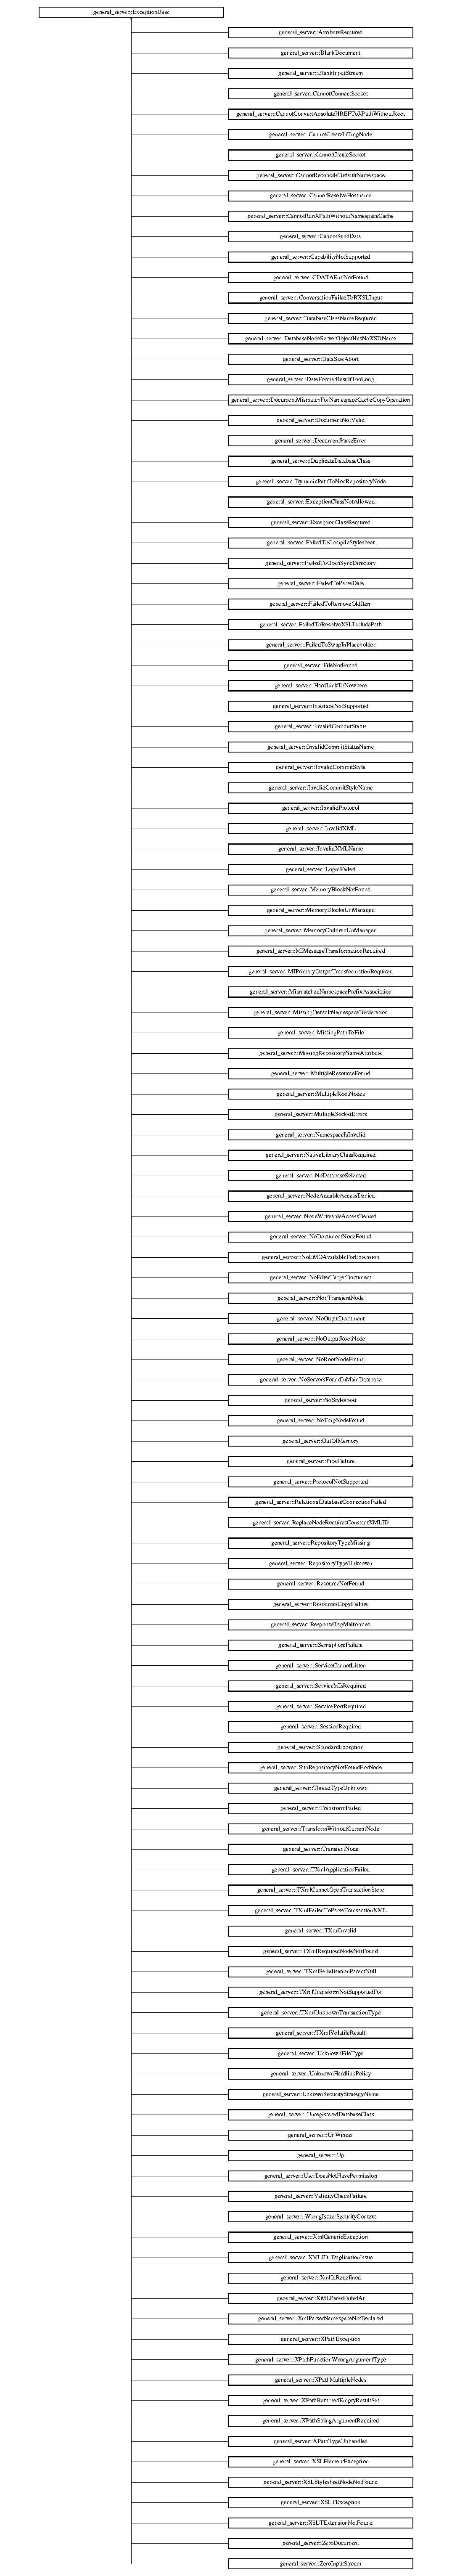
\includegraphics[height=12.000000cm]{classgeneral__server_1_1ExceptionBase}
\end{center}
\end{figure}
\subsection*{\-Public \-Member \-Functions}
\begin{DoxyCompactItemize}
\item 
\hypertarget{classgeneral__server_1_1ExceptionBase_acea12600a93bc94f5d0789b1dc17e2f7}{virtual \hyperlink{classgeneral__server_1_1ExceptionBase}{\-Exception\-Base} $\ast$ {\bfseries clone\-\_\-with\-\_\-resources} () const =0}\label{classgeneral__server_1_1ExceptionBase_acea12600a93bc94f5d0789b1dc17e2f7}

\item 
\hypertarget{classgeneral__server_1_1ExceptionBase_a9809e78cfc96a08c27d683aaebeba5b4}{virtual const char $\ast$ {\bfseries type} () const }\label{classgeneral__server_1_1ExceptionBase_a9809e78cfc96a08c27d683aaebeba5b4}

\item 
\hypertarget{classgeneral__server_1_1ExceptionBase_a1260b54c591de111a206c6139492da2a}{virtual \hyperlink{classgeneral__server_1_1StringMap}{\-String\-Map}$<$ const char $\ast$ $>$ $\ast$ {\bfseries variables} () const }\label{classgeneral__server_1_1ExceptionBase_a1260b54c591de111a206c6139492da2a}

\item 
\hypertarget{classgeneral__server_1_1ExceptionBase_a6d805801cec0b1abfec9cc76e7902e7d}{virtual const char $\ast$ {\bfseries context\-X\-M\-L\-I\-D} ()}\label{classgeneral__server_1_1ExceptionBase_a6d805801cec0b1abfec9cc76e7902e7d}

\item 
\hypertarget{classgeneral__server_1_1ExceptionBase_a353d5732b24946dd6b54f01b3ce2af4a}{const char $\ast$ {\bfseries to\-String} () const }\label{classgeneral__server_1_1ExceptionBase_a353d5732b24946dd6b54f01b3ce2af4a}

\item 
\hypertarget{classgeneral__server_1_1ExceptionBase_a87a3b78556dd3eb35d5457b7c2eceb13}{virtual const char $\ast$ {\bfseries what} () const   throw ()}\label{classgeneral__server_1_1ExceptionBase_a87a3b78556dd3eb35d5457b7c2eceb13}

\item 
\hypertarget{classgeneral__server_1_1ExceptionBase_abed7e254f45b324e3abeb37b76f59dd2}{\hyperlink{classgeneral__server_1_1ExceptionBase}{\-Exception\-Base} $\ast$ {\bfseries nested\-Exception} () const }\label{classgeneral__server_1_1ExceptionBase_abed7e254f45b324e3abeb37b76f59dd2}

\end{DoxyCompactItemize}
\subsection*{\-Static \-Public \-Member \-Functions}
\begin{DoxyCompactItemize}
\item 
\hypertarget{classgeneral__server_1_1ExceptionBase_a8df8baa4f43ea58e92e34f22f25ae00e}{static void {\bfseries factory\-\_\-throw} (const char $\ast$s\-Class, const char $\ast$s\-Parameter1, const char $\ast$s\-Parameter2, const char $\ast$s\-Parameter3)}\label{classgeneral__server_1_1ExceptionBase_a8df8baa4f43ea58e92e34f22f25ae00e}

\item 
\hypertarget{classgeneral__server_1_1ExceptionBase_ad16b262454746a402ec6439989c87fef}{static void {\bfseries compilation\-Information} (const \-I\-Xml\-Query\-Environment $\ast$p\-Q\-E, \-I\-Xml\-Base\-Node $\ast$p\-Output)}\label{classgeneral__server_1_1ExceptionBase_ad16b262454746a402ec6439989c87fef}

\end{DoxyCompactItemize}
\subsection*{\-Protected \-Member \-Functions}
\begin{DoxyCompactItemize}
\item 
\hypertarget{classgeneral__server_1_1ExceptionBase_af62bf8eef88a40391318ed12b81640b9}{{\bfseries \-Exception\-Base} (const bool b\-In\-Catch)}\label{classgeneral__server_1_1ExceptionBase_af62bf8eef88a40391318ed12b81640b9}

\item 
\hypertarget{classgeneral__server_1_1ExceptionBase_ac5fab345b4c044530ae2c002395890ca}{{\bfseries \-Exception\-Base} (const bool b\-In\-Catch, const \hyperlink{classgeneral__server_1_1ExceptionBase}{\-Exception\-Base} \&eb)}\label{classgeneral__server_1_1ExceptionBase_ac5fab345b4c044530ae2c002395890ca}

\item 
\hypertarget{classgeneral__server_1_1ExceptionBase_a063ff8ad01e703048aa7e73bc8658958}{{\bfseries \-Exception\-Base} (const bool b\-In\-Catch, const char $\ast$s\-Message)}\label{classgeneral__server_1_1ExceptionBase_a063ff8ad01e703048aa7e73bc8658958}

\item 
\hypertarget{classgeneral__server_1_1ExceptionBase_a7b05d5dc2ca011f3141005c0b1595cd6}{{\bfseries \-Exception\-Base} (const bool b\-In\-Catch, const char $\ast$s\-Format, const int i\-Param)}\label{classgeneral__server_1_1ExceptionBase_a7b05d5dc2ca011f3141005c0b1595cd6}

\item 
\hypertarget{classgeneral__server_1_1ExceptionBase_a45951786aa1e9cb00decebc88d224ca9}{{\bfseries \-Exception\-Base} (const bool b\-In\-Catch, const char $\ast$s\-Format, const char $\ast$s\-Param1)}\label{classgeneral__server_1_1ExceptionBase_a45951786aa1e9cb00decebc88d224ca9}

\item 
\hypertarget{classgeneral__server_1_1ExceptionBase_a1627ba04681d6ec6432fadd61bdcb1b7}{{\bfseries \-Exception\-Base} (const bool b\-In\-Catch, const char $\ast$s\-Format, const char $\ast$s\-Param1, const char $\ast$s\-Param2)}\label{classgeneral__server_1_1ExceptionBase_a1627ba04681d6ec6432fadd61bdcb1b7}

\item 
\hypertarget{classgeneral__server_1_1ExceptionBase_a517116089f88a00751f63b325c352b5d}{{\bfseries \-Exception\-Base} (const bool b\-In\-Catch, const char $\ast$s\-Format, const char $\ast$s\-Param1, const char $\ast$s\-Param2, const char $\ast$s\-Param3)}\label{classgeneral__server_1_1ExceptionBase_a517116089f88a00751f63b325c352b5d}

\item 
\hypertarget{classgeneral__server_1_1ExceptionBase_a4b2b1a970a8ba3acbef301ebff2f17b3}{void {\bfseries \-Exception\-Base\-\_\-construct} (const bool b\-In\-Catch, const char $\ast$s\-Contructor)}\label{classgeneral__server_1_1ExceptionBase_a4b2b1a970a8ba3acbef301ebff2f17b3}

\item 
\hypertarget{classgeneral__server_1_1ExceptionBase_af322d346dd9a35df346cd960cee7da6e}{{\bfseries \-Exception\-Base} (const \hyperlink{classgeneral__server_1_1ExceptionBase}{\-Exception\-Base} \&eb)}\label{classgeneral__server_1_1ExceptionBase_af322d346dd9a35df346cd960cee7da6e}

\item 
\hypertarget{classgeneral__server_1_1ExceptionBase_a597e5c3f206621e0713d889ca10c0723}{\hyperlink{classgeneral__server_1_1ExceptionBase}{\-Exception\-Base} \& {\bfseries operator=} (const \hyperlink{classgeneral__server_1_1ExceptionBase}{\-Exception\-Base} \&eb)}\label{classgeneral__server_1_1ExceptionBase_a597e5c3f206621e0713d889ca10c0723}

\item 
\hypertarget{classgeneral__server_1_1ExceptionBase_acaa334a0a8dce2d2858973b3a62deea8}{const bool {\bfseries in\-Catch} (const bool b\-In\-Catch)}\label{classgeneral__server_1_1ExceptionBase_acaa334a0a8dce2d2858973b3a62deea8}

\end{DoxyCompactItemize}
\subsection*{\-Protected \-Attributes}
\begin{DoxyCompactItemize}
\item 
\hypertarget{classgeneral__server_1_1ExceptionBase_aab764f7ca0616f0c480921e92d489bc1}{\hyperlink{classgeneral__server_1_1ExceptionBase}{\-Exception\-Base} $\ast$ {\bfseries m\-\_\-p\-E\-X}}\label{classgeneral__server_1_1ExceptionBase_aab764f7ca0616f0c480921e92d489bc1}

\end{DoxyCompactItemize}


\-The documentation for this class was generated from the following files\-:\begin{DoxyCompactItemize}
\item 
platform\-\_\-general/\-Exceptions.\-h\item 
platform\-\_\-general/\-Exceptions.\-cpp\end{DoxyCompactItemize}

\hypertarget{classgeneral__server_1_1ExceptionClassNotAllowed}{\section{general\-\_\-server\-:\-:\-Exception\-Class\-Not\-Allowed \-Class \-Reference}
\label{classgeneral__server_1_1ExceptionClassNotAllowed}\index{general\-\_\-server\-::\-Exception\-Class\-Not\-Allowed@{general\-\_\-server\-::\-Exception\-Class\-Not\-Allowed}}
}
\-Inheritance diagram for general\-\_\-server\-:\-:\-Exception\-Class\-Not\-Allowed\-:\begin{figure}[H]
\begin{center}
\leavevmode
\includegraphics[height=2.000000cm]{classgeneral__server_1_1ExceptionClassNotAllowed}
\end{center}
\end{figure}
\subsection*{\-Public \-Member \-Functions}
\begin{DoxyCompactItemize}
\item 
\hypertarget{classgeneral__server_1_1ExceptionClassNotAllowed_a1e92cce1d46f52269c5d8f5bd006321f}{{\bfseries \-Exception\-Class\-Not\-Allowed} (const char $\ast$s\-Class\-Name=0)}\label{classgeneral__server_1_1ExceptionClassNotAllowed_a1e92cce1d46f52269c5d8f5bd006321f}

\end{DoxyCompactItemize}
\subsection*{\-Protected \-Member \-Functions}
\begin{DoxyCompactItemize}
\item 
\hypertarget{classgeneral__server_1_1ExceptionClassNotAllowed_a58e80a37ff4bdffcb9fe7ba046d42c83}{\hyperlink{classgeneral__server_1_1ExceptionClassNotAllowed}{\-Exception\-Class\-Not\-Allowed} $\ast$ {\bfseries clone\-\_\-with\-\_\-resources} () const }\label{classgeneral__server_1_1ExceptionClassNotAllowed_a58e80a37ff4bdffcb9fe7ba046d42c83}

\end{DoxyCompactItemize}


\-The documentation for this class was generated from the following file\-:\begin{DoxyCompactItemize}
\item 
platform\-\_\-general/\-Exceptions.\-h\end{DoxyCompactItemize}

\hypertarget{classgeneral__server_1_1ExceptionClassRequired}{\section{general\-\_\-server\-:\-:\-Exception\-Class\-Required \-Class \-Reference}
\label{classgeneral__server_1_1ExceptionClassRequired}\index{general\-\_\-server\-::\-Exception\-Class\-Required@{general\-\_\-server\-::\-Exception\-Class\-Required}}
}
\-Inheritance diagram for general\-\_\-server\-:\-:\-Exception\-Class\-Required\-:\begin{figure}[H]
\begin{center}
\leavevmode
\includegraphics[height=2.000000cm]{classgeneral__server_1_1ExceptionClassRequired}
\end{center}
\end{figure}
\subsection*{\-Protected \-Member \-Functions}
\begin{DoxyCompactItemize}
\item 
\hypertarget{classgeneral__server_1_1ExceptionClassRequired_a77e1e37427cabb2be92ced420044d513}{\hyperlink{classgeneral__server_1_1ExceptionClassRequired}{\-Exception\-Class\-Required} $\ast$ {\bfseries clone\-\_\-with\-\_\-resources} () const }\label{classgeneral__server_1_1ExceptionClassRequired_a77e1e37427cabb2be92ced420044d513}

\end{DoxyCompactItemize}


\-The documentation for this class was generated from the following file\-:\begin{DoxyCompactItemize}
\item 
platform\-\_\-general/\-Exceptions.\-h\end{DoxyCompactItemize}

\hypertarget{classgeneral__server_1_1EXSLTRegExp}{\section{general\-\_\-server\-:\-:\-E\-X\-S\-L\-T\-Reg\-Exp \-Class \-Reference}
\label{classgeneral__server_1_1EXSLTRegExp}\index{general\-\_\-server\-::\-E\-X\-S\-L\-T\-Reg\-Exp@{general\-\_\-server\-::\-E\-X\-S\-L\-T\-Reg\-Exp}}
}
\subsection*{\-Public \-Member \-Functions}
\begin{DoxyCompactItemize}
\item 
\hypertarget{classgeneral__server_1_1EXSLTRegExp_a300e6f26384d908ad6d8d9273cf38a95}{const char $\ast$ {\bfseries xslt\-Module\-Namespace} () const }\label{classgeneral__server_1_1EXSLTRegExp_a300e6f26384d908ad6d8d9273cf38a95}

\item 
\hypertarget{classgeneral__server_1_1EXSLTRegExp_a73a170d43249f1237808f10be2bccb05}{const char $\ast$ {\bfseries xslt\-Module\-Prefix} () const }\label{classgeneral__server_1_1EXSLTRegExp_a73a170d43249f1237808f10be2bccb05}

\item 
\hypertarget{classgeneral__server_1_1EXSLTRegExp_ac53783385eaa2336b337a85ff418cf9b}{const \hyperlink{classgeneral__server_1_1StringMap}{\-String\-Map}\*
$<$ \-I\-Xsl\-Module\-::\-Xsl\-Module\-Function\-Details $>$ $\ast$ {\bfseries xsl\-Functions} () const }\label{classgeneral__server_1_1EXSLTRegExp_ac53783385eaa2336b337a85ff418cf9b}

\item 
\hypertarget{classgeneral__server_1_1EXSLTRegExp_a0d5ce1e1cabbe930c7b2123d6cce0849}{const char $\ast$ {\bfseries xsl\-Function\-\_\-replace} (const \-I\-Xml\-Query\-Environment $\ast$p\-Q\-E, const \-I\-Xsl\-X\-Path\-Function\-Context $\ast$p\-X\-Ctxt, \hyperlink{classgeneral__server_1_1XmlNodeList}{\-Xml\-Node\-List}$<$ const \-I\-Xml\-Base\-Node $>$ $\ast$$\ast$p\-Nodes)}\label{classgeneral__server_1_1EXSLTRegExp_a0d5ce1e1cabbe930c7b2123d6cce0849}

\end{DoxyCompactItemize}


\-The documentation for this class was generated from the following files\-:\begin{DoxyCompactItemize}
\item 
platform\-\_\-general/\-Database.\-h\item 
platform\-\_\-general/\-Database.\-cpp\end{DoxyCompactItemize}

\hypertarget{classgeneral__server_1_1EXSLTStrings}{\section{general\-\_\-server\-:\-:\-E\-X\-S\-L\-T\-Strings \-Class \-Reference}
\label{classgeneral__server_1_1EXSLTStrings}\index{general\-\_\-server\-::\-E\-X\-S\-L\-T\-Strings@{general\-\_\-server\-::\-E\-X\-S\-L\-T\-Strings}}
}
\subsection*{\-Public \-Member \-Functions}
\begin{DoxyCompactItemize}
\item 
\hypertarget{classgeneral__server_1_1EXSLTStrings_a8ae8d5948d76abc497d3305f18cf0d0c}{const char $\ast$ {\bfseries xslt\-Module\-Namespace} () const }\label{classgeneral__server_1_1EXSLTStrings_a8ae8d5948d76abc497d3305f18cf0d0c}

\item 
\hypertarget{classgeneral__server_1_1EXSLTStrings_ab76a19a644e766c8cb549cf669aeff1f}{const char $\ast$ {\bfseries xslt\-Module\-Prefix} () const }\label{classgeneral__server_1_1EXSLTStrings_ab76a19a644e766c8cb549cf669aeff1f}

\item 
\hypertarget{classgeneral__server_1_1EXSLTStrings_ab944564bd7b00a0023b8523800f683bf}{const \hyperlink{classgeneral__server_1_1StringMap}{\-String\-Map}\*
$<$ \-I\-Xsl\-Module\-::\-Xsl\-Module\-Function\-Details $>$ $\ast$ {\bfseries xsl\-Functions} () const }\label{classgeneral__server_1_1EXSLTStrings_ab944564bd7b00a0023b8523800f683bf}

\item 
\hypertarget{classgeneral__server_1_1EXSLTStrings_a4bce1e6a7bd59d0f7ddd12ff089b3c5c}{const char $\ast$ {\bfseries xsl\-Function\-\_\-substring\-After\-Last} (const \-I\-Xml\-Query\-Environment $\ast$p\-Q\-E, const \-I\-Xsl\-X\-Path\-Function\-Context $\ast$p\-X\-Ctxt, \hyperlink{classgeneral__server_1_1XmlNodeList}{\-Xml\-Node\-List}$<$ const \-I\-Xml\-Base\-Node $>$ $\ast$$\ast$p\-Nodes)}\label{classgeneral__server_1_1EXSLTStrings_a4bce1e6a7bd59d0f7ddd12ff089b3c5c}

\item 
\hypertarget{classgeneral__server_1_1EXSLTStrings_a17af910629c7535b412db74b44a64d59}{const char $\ast$ {\bfseries xsl\-Function\-\_\-substring\-Before\-Last} (const \-I\-Xml\-Query\-Environment $\ast$p\-Q\-E, const \-I\-Xsl\-X\-Path\-Function\-Context $\ast$p\-X\-Ctxt, \hyperlink{classgeneral__server_1_1XmlNodeList}{\-Xml\-Node\-List}$<$ const \-I\-Xml\-Base\-Node $>$ $\ast$$\ast$p\-Nodes)}\label{classgeneral__server_1_1EXSLTStrings_a17af910629c7535b412db74b44a64d59}

\item 
\hypertarget{classgeneral__server_1_1EXSLTStrings_a775c3d18492ca55acfa54cbdf67e5df9}{const char $\ast$ {\bfseries xsl\-Function\-\_\-substring\-After} (const \-I\-Xml\-Query\-Environment $\ast$p\-Q\-E, const \-I\-Xsl\-X\-Path\-Function\-Context $\ast$p\-X\-Ctxt, \hyperlink{classgeneral__server_1_1XmlNodeList}{\-Xml\-Node\-List}$<$ const \-I\-Xml\-Base\-Node $>$ $\ast$$\ast$p\-Nodes)}\label{classgeneral__server_1_1EXSLTStrings_a775c3d18492ca55acfa54cbdf67e5df9}

\item 
\hypertarget{classgeneral__server_1_1EXSLTStrings_abd83e9c77651d77625d3906123be06da}{const char $\ast$ {\bfseries xsl\-Function\-\_\-substring\-Before} (const \-I\-Xml\-Query\-Environment $\ast$p\-Q\-E, const \-I\-Xsl\-X\-Path\-Function\-Context $\ast$p\-X\-Ctxt, \hyperlink{classgeneral__server_1_1XmlNodeList}{\-Xml\-Node\-List}$<$ const \-I\-Xml\-Base\-Node $>$ $\ast$$\ast$p\-Nodes)}\label{classgeneral__server_1_1EXSLTStrings_abd83e9c77651d77625d3906123be06da}

\item 
\hypertarget{classgeneral__server_1_1EXSLTStrings_a3075afe573fa456e114c044888c7398c}{const char $\ast$ {\bfseries xsl\-Function\-\_\-boolean} (const \-I\-Xml\-Query\-Environment $\ast$p\-Q\-E, const \-I\-Xsl\-X\-Path\-Function\-Context $\ast$p\-X\-Ctxt, \hyperlink{classgeneral__server_1_1XmlNodeList}{\-Xml\-Node\-List}$<$ const \-I\-Xml\-Base\-Node $>$ $\ast$$\ast$p\-Nodes)}\label{classgeneral__server_1_1EXSLTStrings_a3075afe573fa456e114c044888c7398c}

\item 
\hypertarget{classgeneral__server_1_1EXSLTStrings_adbc5a757753ceecc89bb3522782d2d43}{const char $\ast$ {\bfseries xsl\-Function\-\_\-not} (const \-I\-Xml\-Query\-Environment $\ast$p\-Q\-E, const \-I\-Xsl\-X\-Path\-Function\-Context $\ast$p\-X\-Ctxt, \hyperlink{classgeneral__server_1_1XmlNodeList}{\-Xml\-Node\-List}$<$ const \-I\-Xml\-Base\-Node $>$ $\ast$$\ast$p\-Nodes)}\label{classgeneral__server_1_1EXSLTStrings_adbc5a757753ceecc89bb3522782d2d43}

\item 
\hypertarget{classgeneral__server_1_1EXSLTStrings_a7137a5d7e4f579480bb617b0cc4c9a35}{const char $\ast$ {\bfseries xsl\-Function\-\_\-dynamic} (const \-I\-Xml\-Query\-Environment $\ast$p\-Q\-E, const \-I\-Xsl\-X\-Path\-Function\-Context $\ast$p\-X\-Ctxt, \hyperlink{classgeneral__server_1_1XmlNodeList}{\-Xml\-Node\-List}$<$ const \-I\-Xml\-Base\-Node $>$ $\ast$$\ast$p\-Nodes)}\label{classgeneral__server_1_1EXSLTStrings_a7137a5d7e4f579480bb617b0cc4c9a35}

\end{DoxyCompactItemize}


\-The documentation for this class was generated from the following files\-:\begin{DoxyCompactItemize}
\item 
platform\-\_\-general/\-Database.\-h\item 
platform\-\_\-general/\-Database.\-cpp\end{DoxyCompactItemize}

\hypertarget{classgeneral__server_1_1FailedToCompileStylesheet}{\section{general\-\_\-server\-:\-:\-Failed\-To\-Compile\-Stylesheet \-Class \-Reference}
\label{classgeneral__server_1_1FailedToCompileStylesheet}\index{general\-\_\-server\-::\-Failed\-To\-Compile\-Stylesheet@{general\-\_\-server\-::\-Failed\-To\-Compile\-Stylesheet}}
}
\-Inheritance diagram for general\-\_\-server\-:\-:\-Failed\-To\-Compile\-Stylesheet\-:\begin{figure}[H]
\begin{center}
\leavevmode
\includegraphics[height=2.000000cm]{classgeneral__server_1_1FailedToCompileStylesheet}
\end{center}
\end{figure}
\subsection*{\-Protected \-Member \-Functions}
\begin{DoxyCompactItemize}
\item 
\hypertarget{classgeneral__server_1_1FailedToCompileStylesheet_a86bba4f3edbf691694da309795ae9244}{\hyperlink{classgeneral__server_1_1FailedToCompileStylesheet}{\-Failed\-To\-Compile\-Stylesheet} $\ast$ {\bfseries clone\-\_\-with\-\_\-resources} () const }\label{classgeneral__server_1_1FailedToCompileStylesheet_a86bba4f3edbf691694da309795ae9244}

\end{DoxyCompactItemize}


\-The documentation for this class was generated from the following file\-:\begin{DoxyCompactItemize}
\item 
platform\-\_\-general/\-Exceptions.\-h\end{DoxyCompactItemize}

\hypertarget{classgeneral__server_1_1FailedToOpenSyncDirectory}{\section{general\-\_\-server\-:\-:\-Failed\-To\-Open\-Sync\-Directory \-Class \-Reference}
\label{classgeneral__server_1_1FailedToOpenSyncDirectory}\index{general\-\_\-server\-::\-Failed\-To\-Open\-Sync\-Directory@{general\-\_\-server\-::\-Failed\-To\-Open\-Sync\-Directory}}
}
\-Inheritance diagram for general\-\_\-server\-:\-:\-Failed\-To\-Open\-Sync\-Directory\-:\begin{figure}[H]
\begin{center}
\leavevmode
\includegraphics[height=2.000000cm]{classgeneral__server_1_1FailedToOpenSyncDirectory}
\end{center}
\end{figure}
\subsection*{\-Public \-Member \-Functions}
\begin{DoxyCompactItemize}
\item 
\hypertarget{classgeneral__server_1_1FailedToOpenSyncDirectory_a076f1ee5953f9171d62d2697b6e6713b}{{\bfseries \-Failed\-To\-Open\-Sync\-Directory} (const char $\ast$s\-Full\-Path)}\label{classgeneral__server_1_1FailedToOpenSyncDirectory_a076f1ee5953f9171d62d2697b6e6713b}

\end{DoxyCompactItemize}
\subsection*{\-Protected \-Member \-Functions}
\begin{DoxyCompactItemize}
\item 
\hypertarget{classgeneral__server_1_1FailedToOpenSyncDirectory_ae1b352a6a59e427cd0f2c804c8fdf7d0}{\hyperlink{classgeneral__server_1_1FailedToOpenSyncDirectory}{\-Failed\-To\-Open\-Sync\-Directory} $\ast$ {\bfseries clone\-\_\-with\-\_\-resources} () const }\label{classgeneral__server_1_1FailedToOpenSyncDirectory_ae1b352a6a59e427cd0f2c804c8fdf7d0}

\end{DoxyCompactItemize}


\-The documentation for this class was generated from the following file\-:\begin{DoxyCompactItemize}
\item 
platform\-\_\-general/\-Exceptions.\-h\end{DoxyCompactItemize}

\hypertarget{classgeneral__server_1_1FailedToParseDate}{\section{general\-\_\-server\-:\-:\-Failed\-To\-Parse\-Date \-Class \-Reference}
\label{classgeneral__server_1_1FailedToParseDate}\index{general\-\_\-server\-::\-Failed\-To\-Parse\-Date@{general\-\_\-server\-::\-Failed\-To\-Parse\-Date}}
}
\-Inheritance diagram for general\-\_\-server\-:\-:\-Failed\-To\-Parse\-Date\-:\begin{figure}[H]
\begin{center}
\leavevmode
\includegraphics[height=2.000000cm]{classgeneral__server_1_1FailedToParseDate}
\end{center}
\end{figure}
\subsection*{\-Public \-Member \-Functions}
\begin{DoxyCompactItemize}
\item 
\hypertarget{classgeneral__server_1_1FailedToParseDate_a5fb9e64935d9911d26c92fb0a86b43d5}{{\bfseries \-Failed\-To\-Parse\-Date} (const char $\ast$s\-Value)}\label{classgeneral__server_1_1FailedToParseDate_a5fb9e64935d9911d26c92fb0a86b43d5}

\end{DoxyCompactItemize}
\subsection*{\-Protected \-Member \-Functions}
\begin{DoxyCompactItemize}
\item 
\hypertarget{classgeneral__server_1_1FailedToParseDate_a9aa05ad241fe436d75c51359218891ce}{\hyperlink{classgeneral__server_1_1FailedToParseDate}{\-Failed\-To\-Parse\-Date} $\ast$ {\bfseries clone\-\_\-with\-\_\-resources} () const }\label{classgeneral__server_1_1FailedToParseDate_a9aa05ad241fe436d75c51359218891ce}

\end{DoxyCompactItemize}


\-The documentation for this class was generated from the following file\-:\begin{DoxyCompactItemize}
\item 
platform\-\_\-general/\-Exceptions.\-h\end{DoxyCompactItemize}

\hypertarget{classgeneral__server_1_1FailedToRemoveOldItem}{\section{general\-\_\-server\-:\-:\-Failed\-To\-Remove\-Old\-Item \-Class \-Reference}
\label{classgeneral__server_1_1FailedToRemoveOldItem}\index{general\-\_\-server\-::\-Failed\-To\-Remove\-Old\-Item@{general\-\_\-server\-::\-Failed\-To\-Remove\-Old\-Item}}
}
\-Inheritance diagram for general\-\_\-server\-:\-:\-Failed\-To\-Remove\-Old\-Item\-:\begin{figure}[H]
\begin{center}
\leavevmode
\includegraphics[height=2.000000cm]{classgeneral__server_1_1FailedToRemoveOldItem}
\end{center}
\end{figure}
\subsection*{\-Public \-Member \-Functions}
\begin{DoxyCompactItemize}
\item 
\hypertarget{classgeneral__server_1_1FailedToRemoveOldItem_a3746b458128fbc1215def8e4d54dff36}{{\bfseries \-Failed\-To\-Remove\-Old\-Item} (const char $\ast$s\-To\-Full\-Path, const int i\-Errno)}\label{classgeneral__server_1_1FailedToRemoveOldItem_a3746b458128fbc1215def8e4d54dff36}

\end{DoxyCompactItemize}
\subsection*{\-Protected \-Member \-Functions}
\begin{DoxyCompactItemize}
\item 
\hypertarget{classgeneral__server_1_1FailedToRemoveOldItem_a2b5c5416c711ef2abeb1612a301c7c16}{\hyperlink{classgeneral__server_1_1FailedToRemoveOldItem}{\-Failed\-To\-Remove\-Old\-Item} $\ast$ {\bfseries clone\-\_\-with\-\_\-resources} () const }\label{classgeneral__server_1_1FailedToRemoveOldItem_a2b5c5416c711ef2abeb1612a301c7c16}

\end{DoxyCompactItemize}


\-The documentation for this class was generated from the following file\-:\begin{DoxyCompactItemize}
\item 
platform\-\_\-general/\-Exceptions.\-h\end{DoxyCompactItemize}

\hypertarget{classgeneral__server_1_1FailedToResolveXSLIncludePath}{\section{general\-\_\-server\-:\-:\-Failed\-To\-Resolve\-X\-S\-L\-Include\-Path \-Class \-Reference}
\label{classgeneral__server_1_1FailedToResolveXSLIncludePath}\index{general\-\_\-server\-::\-Failed\-To\-Resolve\-X\-S\-L\-Include\-Path@{general\-\_\-server\-::\-Failed\-To\-Resolve\-X\-S\-L\-Include\-Path}}
}
\-Inheritance diagram for general\-\_\-server\-:\-:\-Failed\-To\-Resolve\-X\-S\-L\-Include\-Path\-:\begin{figure}[H]
\begin{center}
\leavevmode
\includegraphics[height=2.000000cm]{classgeneral__server_1_1FailedToResolveXSLIncludePath}
\end{center}
\end{figure}
\subsection*{\-Public \-Member \-Functions}
\begin{DoxyCompactItemize}
\item 
\hypertarget{classgeneral__server_1_1FailedToResolveXSLIncludePath_a1a75b302e8d7820d98596b698e042230}{{\bfseries \-Failed\-To\-Resolve\-X\-S\-L\-Include\-Path} (const char $\ast$s\-X\-Path)}\label{classgeneral__server_1_1FailedToResolveXSLIncludePath_a1a75b302e8d7820d98596b698e042230}

\end{DoxyCompactItemize}
\subsection*{\-Protected \-Member \-Functions}
\begin{DoxyCompactItemize}
\item 
\hypertarget{classgeneral__server_1_1FailedToResolveXSLIncludePath_a163cf1dbec07cdeaa6199af7899da83c}{\hyperlink{classgeneral__server_1_1FailedToResolveXSLIncludePath}{\-Failed\-To\-Resolve\-X\-S\-L\-Include\-Path} $\ast$ {\bfseries clone\-\_\-with\-\_\-resources} () const }\label{classgeneral__server_1_1FailedToResolveXSLIncludePath_a163cf1dbec07cdeaa6199af7899da83c}

\end{DoxyCompactItemize}


\-The documentation for this class was generated from the following file\-:\begin{DoxyCompactItemize}
\item 
platform\-\_\-general/\-Exceptions.\-h\end{DoxyCompactItemize}

\hypertarget{classgeneral__server_1_1FailedToSwapInPlaceholder}{\section{general\-\_\-server\-:\-:\-Failed\-To\-Swap\-In\-Placeholder \-Class \-Reference}
\label{classgeneral__server_1_1FailedToSwapInPlaceholder}\index{general\-\_\-server\-::\-Failed\-To\-Swap\-In\-Placeholder@{general\-\_\-server\-::\-Failed\-To\-Swap\-In\-Placeholder}}
}
\-Inheritance diagram for general\-\_\-server\-:\-:\-Failed\-To\-Swap\-In\-Placeholder\-:\begin{figure}[H]
\begin{center}
\leavevmode
\includegraphics[height=2.000000cm]{classgeneral__server_1_1FailedToSwapInPlaceholder}
\end{center}
\end{figure}
\subsection*{\-Public \-Member \-Functions}
\begin{DoxyCompactItemize}
\item 
\hypertarget{classgeneral__server_1_1FailedToSwapInPlaceholder_a9e600abc477387b231af936147b7e56c}{{\bfseries \-Failed\-To\-Swap\-In\-Placeholder} (const char $\ast$s\-From\-Full\-Path, const char $\ast$s\-To\-Full\-Path, const int i\-Errno)}\label{classgeneral__server_1_1FailedToSwapInPlaceholder_a9e600abc477387b231af936147b7e56c}

\end{DoxyCompactItemize}
\subsection*{\-Protected \-Member \-Functions}
\begin{DoxyCompactItemize}
\item 
\hypertarget{classgeneral__server_1_1FailedToSwapInPlaceholder_a2f1391cb4a959d5a4acb09c92469c9a8}{\hyperlink{classgeneral__server_1_1FailedToSwapInPlaceholder}{\-Failed\-To\-Swap\-In\-Placeholder} $\ast$ {\bfseries clone\-\_\-with\-\_\-resources} () const }\label{classgeneral__server_1_1FailedToSwapInPlaceholder_a2f1391cb4a959d5a4acb09c92469c9a8}

\end{DoxyCompactItemize}


\-The documentation for this class was generated from the following file\-:\begin{DoxyCompactItemize}
\item 
platform\-\_\-general/\-Exceptions.\-h\end{DoxyCompactItemize}

\hypertarget{classgeneral__server_1_1File}{\section{general\-\_\-server\-:\-:\-File \-Class \-Reference}
\label{classgeneral__server_1_1File}\index{general\-\_\-server\-::\-File@{general\-\_\-server\-::\-File}}
}
\-Inheritance diagram for general\-\_\-server\-:\-:\-File\-:\begin{figure}[H]
\begin{center}
\leavevmode
\includegraphics[height=1.887640cm]{classgeneral__server_1_1File}
\end{center}
\end{figure}
\subsection*{\-Public \-Member \-Functions}
\begin{DoxyCompactItemize}
\item 
\hypertarget{classgeneral__server_1_1File_ae36ccfff166c646ce240fa53a79b96bc}{{\bfseries \-File} (const \-I\-Xml\-Library $\ast$p\-Lib, const char $\ast$s\-Full\-Path, const \hyperlink{classgeneral__server_1_1Repository}{\-Repository} $\ast$p\-Parent=\-N\-U\-L\-L)}\label{classgeneral__server_1_1File_ae36ccfff166c646ce240fa53a79b96bc}

\item 
\hypertarget{classgeneral__server_1_1File_a56a3940f42e4011378b9ace0919b55d6}{{\bfseries \-File} (const \-I\-Xml\-Library $\ast$p\-Lib, const \hyperlink{classgeneral__server_1_1DatabaseNode}{\-Database\-Node} $\ast$p\-Node, const \hyperlink{classgeneral__server_1_1Repository}{\-Repository} $\ast$p\-Root\-Repository)}\label{classgeneral__server_1_1File_a56a3940f42e4011378b9ace0919b55d6}

\item 
\hypertarget{classgeneral__server_1_1File_ac6bb715ace08c33255073625e486a45c}{void {\bfseries append\-Xml\-To\-\_\-content} (string \&s\-Current\-X\-M\-L, const bool b\-Is\-Top=false) const }\label{classgeneral__server_1_1File_ac6bb715ace08c33255073625e486a45c}

\item 
\hypertarget{classgeneral__server_1_1File_a07e11dd084d6554e1df16053853c17ff}{void {\bfseries save\-As} (const char $\ast$s\-Full\-Path) const }\label{classgeneral__server_1_1File_a07e11dd084d6554e1df16053853c17ff}

\item 
\hypertarget{classgeneral__server_1_1File_ab416d27bce2bee3fe44430241441e99b}{const char $\ast$ {\bfseries read\-Raw} () const }\label{classgeneral__server_1_1File_ab416d27bce2bee3fe44430241441e99b}

\item 
\hypertarget{classgeneral__server_1_1File_ae8850652decb8390cbcaaef98b79d6e2}{\hyperlink{classvector}{vector}$<$ char $>$ $\ast$ {\bfseries read\-Binary} () const }\label{classgeneral__server_1_1File_ae8850652decb8390cbcaaef98b79d6e2}

\item 
\hypertarget{classgeneral__server_1_1File_a9709cd35f1381e140e77b0cd79c6ca21}{const bool {\bfseries remove\-During\-Sync} () const }\label{classgeneral__server_1_1File_a9709cd35f1381e140e77b0cd79c6ca21}

\item 
\hypertarget{classgeneral__server_1_1File_a4db4849378821e3afdb59c03b02d53d4}{const \-Repository\-::repository\-Type {\bfseries type} () const }\label{classgeneral__server_1_1File_a4db4849378821e3afdb59c03b02d53d4}

\item 
\hypertarget{classgeneral__server_1_1File_a019a5c9cb0732e83e89e825c8172b475}{const \-T\-Xml\-::transaction\-Result {\bfseries create\-Save\-Tree\-Placeholder} (const bool b\-Add\-Placeholder\-Prefix=true)}\label{classgeneral__server_1_1File_a019a5c9cb0732e83e89e825c8172b475}

\item 
\hypertarget{classgeneral__server_1_1File_a148ef8d0071439cf8a76f1519a9862eb}{const \-T\-Xml\-::transaction\-Result {\bfseries swap\-In\-Save\-Tree\-Placeholder} ()}\label{classgeneral__server_1_1File_a148ef8d0071439cf8a76f1519a9862eb}

\end{DoxyCompactItemize}
\subsection*{\-Static \-Public \-Member \-Functions}
\begin{DoxyCompactItemize}
\item 
\hypertarget{classgeneral__server_1_1File_a077ecb65923583802054dd639ed93f88}{static const bool {\bfseries gimme} (const char $\ast$s\-File\-Path)}\label{classgeneral__server_1_1File_a077ecb65923583802054dd639ed93f88}

\item 
\hypertarget{classgeneral__server_1_1File_ac87dfe8bed5076bcfd2191754355068b}{static void {\bfseries compilation\-Information} (const \-I\-Xml\-Query\-Environment $\ast$p\-Q\-E, \-I\-Xml\-Base\-Node $\ast$p\-Output)}\label{classgeneral__server_1_1File_ac87dfe8bed5076bcfd2191754355068b}

\end{DoxyCompactItemize}
\subsection*{\-Static \-Public \-Attributes}
\begin{DoxyCompactItemize}
\item 
\hypertarget{classgeneral__server_1_1File_aa83dcf1be85523291274a7a4945247fd}{static const char $\ast$ {\bfseries m\-\_\-s\-Type\-Name} = \char`\"{}\-File\char`\"{}}\label{classgeneral__server_1_1File_aa83dcf1be85523291274a7a4945247fd}

\end{DoxyCompactItemize}
\subsection*{\-Protected \-Member \-Functions}
\begin{DoxyCompactItemize}
\item 
\hypertarget{classgeneral__server_1_1File_a7b8e47cf25458a9c98b65ef0b944c4ff}{void {\bfseries read\-Valid\-X\-M\-L} (string \&s\-Current\-X\-M\-L) const }\label{classgeneral__server_1_1File_a7b8e47cf25458a9c98b65ef0b944c4ff}

\item 
\hypertarget{classgeneral__server_1_1File_aa700d21d8770be803002a519c53be859}{const char $\ast$ {\bfseries placeholder\-Name} (const bool b\-Add\-Placeholder\-Prefix) const }\label{classgeneral__server_1_1File_aa700d21d8770be803002a519c53be859}

\end{DoxyCompactItemize}
\subsection*{\-Static \-Protected \-Attributes}
\begin{DoxyCompactItemize}
\item 
\hypertarget{classgeneral__server_1_1File_a68e7ab3dd702780bd243bfd6553cdec6}{static const \*
\-Repository\-::repository\-Type {\bfseries m\-\_\-i\-Repository\-Type} = t\-File}\label{classgeneral__server_1_1File_a68e7ab3dd702780bd243bfd6553cdec6}

\end{DoxyCompactItemize}
\subsection*{\-Friends}
\begin{DoxyCompactItemize}
\item 
\hypertarget{classgeneral__server_1_1File_a245303e8660be5fb8eb2828a8c44b773}{class {\bfseries \-Directory}}\label{classgeneral__server_1_1File_a245303e8660be5fb8eb2828a8c44b773}

\end{DoxyCompactItemize}


\-The documentation for this class was generated from the following files\-:\begin{DoxyCompactItemize}
\item 
platform\-\_\-general/\-File\-System.\-h\item 
platform\-\_\-general/\-File\-System.\-cpp\end{DoxyCompactItemize}

\hypertarget{classgeneral__server_1_1FileNotFound}{\section{general\-\_\-server\-:\-:\-File\-Not\-Found \-Class \-Reference}
\label{classgeneral__server_1_1FileNotFound}\index{general\-\_\-server\-::\-File\-Not\-Found@{general\-\_\-server\-::\-File\-Not\-Found}}
}
\-Inheritance diagram for general\-\_\-server\-:\-:\-File\-Not\-Found\-:\begin{figure}[H]
\begin{center}
\leavevmode
\includegraphics[height=2.000000cm]{classgeneral__server_1_1FileNotFound}
\end{center}
\end{figure}
\subsection*{\-Public \-Member \-Functions}
\begin{DoxyCompactItemize}
\item 
\hypertarget{classgeneral__server_1_1FileNotFound_ab2e6b14eacc5275da0e7b85d6d138f47}{{\bfseries \-File\-Not\-Found} (const char $\ast$s\-Full\-Path)}\label{classgeneral__server_1_1FileNotFound_ab2e6b14eacc5275da0e7b85d6d138f47}

\end{DoxyCompactItemize}
\subsection*{\-Protected \-Member \-Functions}
\begin{DoxyCompactItemize}
\item 
\hypertarget{classgeneral__server_1_1FileNotFound_a21ab27b8d6f68626cdf01bb367fe3c86}{\hyperlink{classgeneral__server_1_1FileNotFound}{\-File\-Not\-Found} $\ast$ {\bfseries clone\-\_\-with\-\_\-resources} () const }\label{classgeneral__server_1_1FileNotFound_a21ab27b8d6f68626cdf01bb367fe3c86}

\end{DoxyCompactItemize}


\-The documentation for this class was generated from the following file\-:\begin{DoxyCompactItemize}
\item 
platform\-\_\-general/\-Exceptions.\-h\end{DoxyCompactItemize}

\hypertarget{classgeneral__server_1_1GeneralServerDatabaseNodeServerObject}{\section{general\-\_\-server\-:\-:\-General\-Server\-Database\-Node\-Server\-Object \-Class \-Reference}
\label{classgeneral__server_1_1GeneralServerDatabaseNodeServerObject}\index{general\-\_\-server\-::\-General\-Server\-Database\-Node\-Server\-Object@{general\-\_\-server\-::\-General\-Server\-Database\-Node\-Server\-Object}}
}
\-Inheritance diagram for general\-\_\-server\-:\-:\-General\-Server\-Database\-Node\-Server\-Object\-:\begin{figure}[H]
\begin{center}
\leavevmode
\includegraphics[height=8.651686cm]{classgeneral__server_1_1GeneralServerDatabaseNodeServerObject}
\end{center}
\end{figure}
\subsection*{\-Public \-Member \-Functions}
\begin{DoxyCompactItemize}
\item 
\hypertarget{classgeneral__server_1_1GeneralServerDatabaseNodeServerObject_a0df3e7984dc67d81b05c1e1ef825e445}{void {\bfseries relinquish\-Database\-Node} ()}\label{classgeneral__server_1_1GeneralServerDatabaseNodeServerObject_a0df3e7984dc67d81b05c1e1ef825e445}

\item 
\hypertarget{classgeneral__server_1_1GeneralServerDatabaseNodeServerObject_acb479b76d842ba89a3ab35f482bdb4c2}{void {\bfseries set\-Database\-Node} (\hyperlink{classgeneral__server_1_1DatabaseNode}{\-Database\-Node} $\ast$p\-Node)}\label{classgeneral__server_1_1GeneralServerDatabaseNodeServerObject_acb479b76d842ba89a3ab35f482bdb4c2}

\end{DoxyCompactItemize}
\subsection*{\-Static \-Public \-Member \-Functions}
\begin{DoxyCompactItemize}
\item 
\hypertarget{classgeneral__server_1_1GeneralServerDatabaseNodeServerObject_a3e20bc30f59eadfb67d76a3e758c8b8e}{static void {\bfseries compilation\-Information} (const \-I\-Xml\-Query\-Environment $\ast$p\-Q\-E, \-I\-Xml\-Base\-Node $\ast$p\-Output)}\label{classgeneral__server_1_1GeneralServerDatabaseNodeServerObject_a3e20bc30f59eadfb67d76a3e758c8b8e}

\end{DoxyCompactItemize}
\subsection*{\-Protected \-Member \-Functions}
\begin{DoxyCompactItemize}
\item 
\hypertarget{classgeneral__server_1_1GeneralServerDatabaseNodeServerObject_a9ed0747ffb0b25db0721201018d5919f}{{\bfseries \-General\-Server\-Database\-Node\-Server\-Object} (\hyperlink{classgeneral__server_1_1DatabaseNode}{\-Database\-Node} $\ast$p\-Node)}\label{classgeneral__server_1_1GeneralServerDatabaseNodeServerObject_a9ed0747ffb0b25db0721201018d5919f}

\item 
\hypertarget{classgeneral__server_1_1GeneralServerDatabaseNodeServerObject_aa01493e54bf2084f5cc9708869846018}{{\bfseries \-General\-Server\-Database\-Node\-Server\-Object} (const \hyperlink{classgeneral__server_1_1DatabaseNode}{\-Database\-Node} $\ast$p\-Node)}\label{classgeneral__server_1_1GeneralServerDatabaseNodeServerObject_aa01493e54bf2084f5cc9708869846018}

\end{DoxyCompactItemize}
\subsection*{\-Protected \-Attributes}
\begin{DoxyCompactItemize}
\item 
\hypertarget{classgeneral__server_1_1GeneralServerDatabaseNodeServerObject_a395d52133cfb28af82820ff4d174f62d}{\hyperlink{classgeneral__server_1_1XmlAdminQueryEnvironment}{\-Xml\-Admin\-Query\-Environment} $\ast$ {\bfseries m\-\_\-p\-I\-B\-Q\-E\-\_\-server\-Startup}}\label{classgeneral__server_1_1GeneralServerDatabaseNodeServerObject_a395d52133cfb28af82820ff4d174f62d}

\end{DoxyCompactItemize}


\-The documentation for this class was generated from the following files\-:\begin{DoxyCompactItemize}
\item 
platform\-\_\-general/\-Database\-Node\-Server\-Object.\-h\item 
platform\-\_\-general/\-Database\-Node\-Server\-Object.\-cpp\end{DoxyCompactItemize}

\hypertarget{classgeneral__server_1_1MessageInterpretation_1_1GimmePred}{\section{general\-\_\-server\-:\-:\-Message\-Interpretation\-:\-:\-Gimme\-Pred \-Class \-Reference}
\label{classgeneral__server_1_1MessageInterpretation_1_1GimmePred}\index{general\-\_\-server\-::\-Message\-Interpretation\-::\-Gimme\-Pred@{general\-\_\-server\-::\-Message\-Interpretation\-::\-Gimme\-Pred}}
}
\subsection*{\-Public \-Member \-Functions}
\begin{DoxyCompactItemize}
\item 
\hypertarget{classgeneral__server_1_1MessageInterpretation_1_1GimmePred_ad559e006a9617b560c569e951496393c}{{\bfseries \-Gimme\-Pred} (const char $\ast$s\-Text\-Stream)}\label{classgeneral__server_1_1MessageInterpretation_1_1GimmePred_ad559e006a9617b560c569e951496393c}

\item 
\hypertarget{classgeneral__server_1_1MessageInterpretation_1_1GimmePred_aedbb080e0be96770aef75800b00f307f}{const bool {\bfseries operator()} (const \hyperlink{classgeneral__server_1_1MessageInterpretation}{\-Message\-Interpretation} $\ast$mi) const }\label{classgeneral__server_1_1MessageInterpretation_1_1GimmePred_aedbb080e0be96770aef75800b00f307f}

\end{DoxyCompactItemize}


\-The documentation for this class was generated from the following file\-:\begin{DoxyCompactItemize}
\item 
platform\-\_\-general/\-Message\-Interpretation.\-h\end{DoxyCompactItemize}

\hypertarget{classgeneral__server_1_1Hardlink}{\section{general\-\_\-server\-:\-:\-Hardlink \-Class \-Reference}
\label{classgeneral__server_1_1Hardlink}\index{general\-\_\-server\-::\-Hardlink@{general\-\_\-server\-::\-Hardlink}}
}
\-Inheritance diagram for general\-\_\-server\-:\-:\-Hardlink\-:\begin{figure}[H]
\begin{center}
\leavevmode
\includegraphics[height=2.621723cm]{classgeneral__server_1_1Hardlink}
\end{center}
\end{figure}
\subsection*{\-Public \-Member \-Functions}
\begin{DoxyCompactItemize}
\item 
\hypertarget{classgeneral__server_1_1Hardlink_abfada1ee9966c30c900d4204ae7dde23}{{\bfseries \-Hardlink} (const \-I\-Xml\-Library $\ast$p\-Lib, const char $\ast$s\-Full\-Path, const \hyperlink{classgeneral__server_1_1Repository}{\-Repository} $\ast$p\-Parent=\-N\-U\-L\-L)}\label{classgeneral__server_1_1Hardlink_abfada1ee9966c30c900d4204ae7dde23}

\item 
\hypertarget{classgeneral__server_1_1Hardlink_aea0a81b89c7bc3ba96a336212d3d2944}{{\bfseries \-Hardlink} (const \-I\-Xml\-Library $\ast$p\-Lib, const \hyperlink{classgeneral__server_1_1DatabaseNode}{\-Database\-Node} $\ast$p\-Node, const \hyperlink{classgeneral__server_1_1Repository}{\-Repository} $\ast$p\-Root\-Repository)}\label{classgeneral__server_1_1Hardlink_aea0a81b89c7bc3ba96a336212d3d2944}

\item 
\hypertarget{classgeneral__server_1_1Hardlink_a2e398006eabf0830b4282634efe39e63}{const bool {\bfseries remove\-During\-Sync} () const }\label{classgeneral__server_1_1Hardlink_a2e398006eabf0830b4282634efe39e63}

\item 
\hypertarget{classgeneral__server_1_1Hardlink_afad7f26300ed8ecdef4ae756af33269e}{const \-Repository\-::repository\-Type {\bfseries type} () const }\label{classgeneral__server_1_1Hardlink_afad7f26300ed8ecdef4ae756af33269e}

\end{DoxyCompactItemize}
\subsection*{\-Static \-Public \-Member \-Functions}
\begin{DoxyCompactItemize}
\item 
\hypertarget{classgeneral__server_1_1Hardlink_a836c5b7a84dad7602c6bfda78e106362}{static const bool {\bfseries gimme} (const char $\ast$s\-File\-Path)}\label{classgeneral__server_1_1Hardlink_a836c5b7a84dad7602c6bfda78e106362}

\item 
\hypertarget{classgeneral__server_1_1Hardlink_a6d24c2209e3c88a5be3fc322412b6b30}{static void {\bfseries compilation\-Information} (const \-I\-Xml\-Query\-Environment $\ast$p\-Q\-E, \-I\-Xml\-Base\-Node $\ast$p\-Output)}\label{classgeneral__server_1_1Hardlink_a6d24c2209e3c88a5be3fc322412b6b30}

\end{DoxyCompactItemize}
\subsection*{\-Static \-Public \-Attributes}
\begin{DoxyCompactItemize}
\item 
\hypertarget{classgeneral__server_1_1Hardlink_ae96633fbfc933f542dc5a573a18ebf82}{static const char $\ast$ {\bfseries m\-\_\-s\-Type\-Name} = \char`\"{}\-Hardlink\char`\"{}}\label{classgeneral__server_1_1Hardlink_ae96633fbfc933f542dc5a573a18ebf82}

\end{DoxyCompactItemize}
\subsection*{\-Static \-Protected \-Attributes}
\begin{DoxyCompactItemize}
\item 
\hypertarget{classgeneral__server_1_1Hardlink_a70b34f078d08bb4edc8005be627ee5aa}{static const \*
\-Repository\-::repository\-Type {\bfseries m\-\_\-i\-Repository\-Type} = t\-Hardlink}\label{classgeneral__server_1_1Hardlink_a70b34f078d08bb4edc8005be627ee5aa}

\end{DoxyCompactItemize}
\subsection*{\-Friends}
\begin{DoxyCompactItemize}
\item 
\hypertarget{classgeneral__server_1_1Hardlink_a245303e8660be5fb8eb2828a8c44b773}{class {\bfseries \-Directory}}\label{classgeneral__server_1_1Hardlink_a245303e8660be5fb8eb2828a8c44b773}

\end{DoxyCompactItemize}


\-The documentation for this class was generated from the following files\-:\begin{DoxyCompactItemize}
\item 
platform\-\_\-general/\-File\-System.\-h\item 
platform\-\_\-general/\-File\-System.\-cpp\end{DoxyCompactItemize}

\hypertarget{classgeneral__server_1_1HardLinkToNowhere}{\section{general\-\_\-server\-:\-:\-Hard\-Link\-To\-Nowhere \-Class \-Reference}
\label{classgeneral__server_1_1HardLinkToNowhere}\index{general\-\_\-server\-::\-Hard\-Link\-To\-Nowhere@{general\-\_\-server\-::\-Hard\-Link\-To\-Nowhere}}
}
\-Inheritance diagram for general\-\_\-server\-:\-:\-Hard\-Link\-To\-Nowhere\-:\begin{figure}[H]
\begin{center}
\leavevmode
\includegraphics[height=2.000000cm]{classgeneral__server_1_1HardLinkToNowhere}
\end{center}
\end{figure}
\subsection*{\-Public \-Member \-Functions}
\begin{DoxyCompactItemize}
\item 
\hypertarget{classgeneral__server_1_1HardLinkToNowhere_a442d6764a999c354d2de7ae742f90e84}{{\bfseries \-Hard\-Link\-To\-Nowhere} (const char $\ast$s\-X\-Path)}\label{classgeneral__server_1_1HardLinkToNowhere_a442d6764a999c354d2de7ae742f90e84}

\end{DoxyCompactItemize}
\subsection*{\-Protected \-Member \-Functions}
\begin{DoxyCompactItemize}
\item 
\hypertarget{classgeneral__server_1_1HardLinkToNowhere_adde3c70e47c2af535cda1a70a6915635}{\hyperlink{classgeneral__server_1_1HardLinkToNowhere}{\-Hard\-Link\-To\-Nowhere} $\ast$ {\bfseries clone\-\_\-with\-\_\-resources} () const }\label{classgeneral__server_1_1HardLinkToNowhere_adde3c70e47c2af535cda1a70a6915635}

\end{DoxyCompactItemize}


\-The documentation for this class was generated from the following file\-:\begin{DoxyCompactItemize}
\item 
platform\-\_\-general/\-Exceptions.\-h\end{DoxyCompactItemize}

\hypertarget{classimplements__interface_01IXmlNodeList}{\section{implements\-\_\-interface \-I\-Xml\-Node\-List \-Class \-Reference}
\label{classimplements__interface_01IXmlNodeList}\index{implements\-\_\-interface I\-Xml\-Node\-List@{implements\-\_\-interface I\-Xml\-Node\-List}}
}
\-Inheritance diagram for implements\-\_\-interface \-I\-Xml\-Node\-List\-:\begin{figure}[H]
\begin{center}
\leavevmode
\includegraphics[height=2.000000cm]{classimplements__interface_01IXmlNodeList}
\end{center}
\end{figure}


\-The documentation for this class was generated from the following file\-:\begin{DoxyCompactItemize}
\item 
platform\-\_\-general/\-Xml/\-Xml\-Node\-List.\-h\end{DoxyCompactItemize}

\hypertarget{classgeneral__server_1_1InterfaceNotSupported}{\section{general\-\_\-server\-:\-:\-Interface\-Not\-Supported \-Class \-Reference}
\label{classgeneral__server_1_1InterfaceNotSupported}\index{general\-\_\-server\-::\-Interface\-Not\-Supported@{general\-\_\-server\-::\-Interface\-Not\-Supported}}
}
\-Inheritance diagram for general\-\_\-server\-:\-:\-Interface\-Not\-Supported\-:\begin{figure}[H]
\begin{center}
\leavevmode
\includegraphics[height=2.000000cm]{classgeneral__server_1_1InterfaceNotSupported}
\end{center}
\end{figure}
\subsection*{\-Public \-Member \-Functions}
\begin{DoxyCompactItemize}
\item 
\hypertarget{classgeneral__server_1_1InterfaceNotSupported_a79a26b93e7d365fb89278db597544283}{{\bfseries \-Interface\-Not\-Supported} (const char $\ast$s\-Class\-Name)}\label{classgeneral__server_1_1InterfaceNotSupported_a79a26b93e7d365fb89278db597544283}

\end{DoxyCompactItemize}
\subsection*{\-Protected \-Member \-Functions}
\begin{DoxyCompactItemize}
\item 
\hypertarget{classgeneral__server_1_1InterfaceNotSupported_a42c8d7b34b8c90c2515717f5a14f38f8}{\hyperlink{classgeneral__server_1_1InterfaceNotSupported}{\-Interface\-Not\-Supported} $\ast$ {\bfseries clone\-\_\-with\-\_\-resources} () const }\label{classgeneral__server_1_1InterfaceNotSupported_a42c8d7b34b8c90c2515717f5a14f38f8}

\end{DoxyCompactItemize}


\-The documentation for this class was generated from the following file\-:\begin{DoxyCompactItemize}
\item 
platform\-\_\-general/\-Exceptions.\-h\end{DoxyCompactItemize}

\hypertarget{classgeneral__server_1_1InternetLocation}{\section{general\-\_\-server\-:\-:\-Internet\-Location \-Class \-Reference}
\label{classgeneral__server_1_1InternetLocation}\index{general\-\_\-server\-::\-Internet\-Location@{general\-\_\-server\-::\-Internet\-Location}}
}
\-Inheritance diagram for general\-\_\-server\-:\-:\-Internet\-Location\-:\begin{figure}[H]
\begin{center}
\leavevmode
\includegraphics[height=2.097378cm]{classgeneral__server_1_1InternetLocation}
\end{center}
\end{figure}
\subsection*{\-Public \-Member \-Functions}
\begin{DoxyCompactItemize}
\item 
\hypertarget{classgeneral__server_1_1InternetLocation_a82377418e028c1add4b90ce004e6d71a}{{\bfseries \-Internet\-Location} (const \-I\-Xml\-Library $\ast$p\-Lib, const char $\ast$s\-Url, const \hyperlink{classgeneral__server_1_1Repository}{\-Repository} $\ast$p\-Parent=\-N\-U\-L\-L)}\label{classgeneral__server_1_1InternetLocation_a82377418e028c1add4b90ce004e6d71a}

\item 
\hypertarget{classgeneral__server_1_1InternetLocation_af36f08a94778e6a13f1c26e0870193e6}{{\bfseries \-Internet\-Location} (const \-I\-Xml\-Library $\ast$p\-Lib, const \hyperlink{classgeneral__server_1_1DatabaseNode}{\-Database\-Node} $\ast$p\-Node, const \hyperlink{classgeneral__server_1_1Repository}{\-Repository} $\ast$p\-Root\-Repository)}\label{classgeneral__server_1_1InternetLocation_af36f08a94778e6a13f1c26e0870193e6}

\item 
\hypertarget{classgeneral__server_1_1InternetLocation_a0f380456c39951004d16d264c7343c05}{const char $\ast$ {\bfseries protocol} () const }\label{classgeneral__server_1_1InternetLocation_a0f380456c39951004d16d264c7343c05}

\item 
\hypertarget{classgeneral__server_1_1InternetLocation_a0caa2e3f2dd432112bb90e06b9e9d60e}{const char $\ast$ {\bfseries hostname} () const }\label{classgeneral__server_1_1InternetLocation_a0caa2e3f2dd432112bb90e06b9e9d60e}

\item 
\hypertarget{classgeneral__server_1_1InternetLocation_a22e88101454da2e60df46d2bb1687fe0}{const char $\ast$ {\bfseries port} () const }\label{classgeneral__server_1_1InternetLocation_a22e88101454da2e60df46d2bb1687fe0}

\item 
\hypertarget{classgeneral__server_1_1InternetLocation_abca91bba58302d0da7b3da84443542da}{const char $\ast$ {\bfseries path} () const }\label{classgeneral__server_1_1InternetLocation_abca91bba58302d0da7b3da84443542da}

\item 
\hypertarget{classgeneral__server_1_1InternetLocation_a5308a8246d4c8005f5bd7b7f155e7a0d}{const char $\ast$ {\bfseries query} () const }\label{classgeneral__server_1_1InternetLocation_a5308a8246d4c8005f5bd7b7f155e7a0d}

\item 
\hypertarget{classgeneral__server_1_1InternetLocation_a9d826a3e6b097a99ded0b799a0438d0c}{const char $\ast$ {\bfseries anchor} () const }\label{classgeneral__server_1_1InternetLocation_a9d826a3e6b097a99ded0b799a0438d0c}

\item 
\hypertarget{classgeneral__server_1_1InternetLocation_ac2773b476327896a3cdf9815be1b4727}{const \-Repository\-::repository\-Type {\bfseries type} () const }\label{classgeneral__server_1_1InternetLocation_ac2773b476327896a3cdf9815be1b4727}

\item 
\hypertarget{classgeneral__server_1_1InternetLocation_a1de3520244087833d8c2aa1bc261fe5f}{const bool {\bfseries remove\-During\-Sync} () const }\label{classgeneral__server_1_1InternetLocation_a1de3520244087833d8c2aa1bc261fe5f}

\item 
\hypertarget{classgeneral__server_1_1InternetLocation_a1bd3d3b385b83b72e0e67afc0a8b0ddf}{const char $\ast$ {\bfseries read\-Raw} () const }\label{classgeneral__server_1_1InternetLocation_a1bd3d3b385b83b72e0e67afc0a8b0ddf}

\item 
\hypertarget{classgeneral__server_1_1InternetLocation_a06af3ea0a6f9ccc4c1c04000a7418353}{void {\bfseries read\-Valid\-X\-M\-L} (string \&s\-Current\-X\-M\-L) const }\label{classgeneral__server_1_1InternetLocation_a06af3ea0a6f9ccc4c1c04000a7418353}

\item 
\hypertarget{classgeneral__server_1_1InternetLocation_ae8b6f621746b4763f275c0f00e770d7c}{void {\bfseries append\-Xml\-To\-\_\-content} (string \&s\-Current\-X\-M\-L, const bool b\-Is\-Top=false) const }\label{classgeneral__server_1_1InternetLocation_ae8b6f621746b4763f275c0f00e770d7c}

\end{DoxyCompactItemize}
\subsection*{\-Static \-Public \-Member \-Functions}
\begin{DoxyCompactItemize}
\item 
\hypertarget{classgeneral__server_1_1InternetLocation_a4ba9882a6792ffa1fd817ea78a60ee1e}{static const bool {\bfseries gimme} (const char $\ast$s\-File\-Path)}\label{classgeneral__server_1_1InternetLocation_a4ba9882a6792ffa1fd817ea78a60ee1e}

\item 
\hypertarget{classgeneral__server_1_1InternetLocation_ad4bf53e302c1ffa6a55889fccc4b27d2}{static void {\bfseries compilation\-Information} (const \-I\-Xml\-Query\-Environment $\ast$p\-Q\-E, \-I\-Xml\-Base\-Node $\ast$p\-Output)}\label{classgeneral__server_1_1InternetLocation_ad4bf53e302c1ffa6a55889fccc4b27d2}

\end{DoxyCompactItemize}
\subsection*{\-Static \-Public \-Attributes}
\begin{DoxyCompactItemize}
\item 
\hypertarget{classgeneral__server_1_1InternetLocation_adfca4cbe80b3d7e7fe4be46fbe9f1e70}{static const char $\ast$ {\bfseries m\-\_\-s\-Type\-Name} = \char`\"{}\-Internet\-Location\char`\"{}}\label{classgeneral__server_1_1InternetLocation_adfca4cbe80b3d7e7fe4be46fbe9f1e70}

\end{DoxyCompactItemize}
\subsection*{\-Static \-Protected \-Attributes}
\begin{DoxyCompactItemize}
\item 
\hypertarget{classgeneral__server_1_1InternetLocation_af6eeaca1eb6f26bdb0b38b03c668ce72}{static const \*
\-Repository\-::repository\-Type {\bfseries m\-\_\-i\-Repository\-Type} = t\-Internet\-Location}\label{classgeneral__server_1_1InternetLocation_af6eeaca1eb6f26bdb0b38b03c668ce72}

\end{DoxyCompactItemize}


\-The documentation for this class was generated from the following files\-:\begin{DoxyCompactItemize}
\item 
platform\-\_\-general/\-File\-System.\-h\item 
platform\-\_\-general/\-File\-System.\-cpp\end{DoxyCompactItemize}

\hypertarget{classgeneral__server_1_1InvalidCommitStatus}{\section{general\-\_\-server\-:\-:\-Invalid\-Commit\-Status \-Class \-Reference}
\label{classgeneral__server_1_1InvalidCommitStatus}\index{general\-\_\-server\-::\-Invalid\-Commit\-Status@{general\-\_\-server\-::\-Invalid\-Commit\-Status}}
}
\-Inheritance diagram for general\-\_\-server\-:\-:\-Invalid\-Commit\-Status\-:\begin{figure}[H]
\begin{center}
\leavevmode
\includegraphics[height=2.000000cm]{classgeneral__server_1_1InvalidCommitStatus}
\end{center}
\end{figure}
\subsection*{\-Public \-Member \-Functions}
\begin{DoxyCompactItemize}
\item 
\hypertarget{classgeneral__server_1_1InvalidCommitStatus_a863107354f0ba4d619616b0998ab982b}{{\bfseries \-Invalid\-Commit\-Status} (const char $\ast$cs)}\label{classgeneral__server_1_1InvalidCommitStatus_a863107354f0ba4d619616b0998ab982b}

\end{DoxyCompactItemize}
\subsection*{\-Protected \-Member \-Functions}
\begin{DoxyCompactItemize}
\item 
\hypertarget{classgeneral__server_1_1InvalidCommitStatus_a1e4cc5e9cdba8c2d069b76a751e929d3}{\hyperlink{classgeneral__server_1_1InvalidCommitStatus}{\-Invalid\-Commit\-Status} $\ast$ {\bfseries clone\-\_\-with\-\_\-resources} () const }\label{classgeneral__server_1_1InvalidCommitStatus_a1e4cc5e9cdba8c2d069b76a751e929d3}

\end{DoxyCompactItemize}


\-The documentation for this class was generated from the following file\-:\begin{DoxyCompactItemize}
\item 
platform\-\_\-general/\-Exceptions.\-h\end{DoxyCompactItemize}

\hypertarget{classgeneral__server_1_1InvalidCommitStatusName}{\section{general\-\_\-server\-:\-:\-Invalid\-Commit\-Status\-Name \-Class \-Reference}
\label{classgeneral__server_1_1InvalidCommitStatusName}\index{general\-\_\-server\-::\-Invalid\-Commit\-Status\-Name@{general\-\_\-server\-::\-Invalid\-Commit\-Status\-Name}}
}
\-Inheritance diagram for general\-\_\-server\-:\-:\-Invalid\-Commit\-Status\-Name\-:\begin{figure}[H]
\begin{center}
\leavevmode
\includegraphics[height=2.000000cm]{classgeneral__server_1_1InvalidCommitStatusName}
\end{center}
\end{figure}
\subsection*{\-Public \-Member \-Functions}
\begin{DoxyCompactItemize}
\item 
\hypertarget{classgeneral__server_1_1InvalidCommitStatusName_a020a2bcc34e981a24c9583798e5bc7e2}{{\bfseries \-Invalid\-Commit\-Status\-Name} (const char $\ast$cs)}\label{classgeneral__server_1_1InvalidCommitStatusName_a020a2bcc34e981a24c9583798e5bc7e2}

\end{DoxyCompactItemize}
\subsection*{\-Protected \-Member \-Functions}
\begin{DoxyCompactItemize}
\item 
\hypertarget{classgeneral__server_1_1InvalidCommitStatusName_a2207ebe2c9992a94dae743910c936167}{\hyperlink{classgeneral__server_1_1InvalidCommitStatusName}{\-Invalid\-Commit\-Status\-Name} $\ast$ {\bfseries clone\-\_\-with\-\_\-resources} () const }\label{classgeneral__server_1_1InvalidCommitStatusName_a2207ebe2c9992a94dae743910c936167}

\end{DoxyCompactItemize}


\-The documentation for this class was generated from the following file\-:\begin{DoxyCompactItemize}
\item 
platform\-\_\-general/\-Exceptions.\-h\end{DoxyCompactItemize}

\hypertarget{classgeneral__server_1_1InvalidCommitStyle}{\section{general\-\_\-server\-:\-:\-Invalid\-Commit\-Style \-Class \-Reference}
\label{classgeneral__server_1_1InvalidCommitStyle}\index{general\-\_\-server\-::\-Invalid\-Commit\-Style@{general\-\_\-server\-::\-Invalid\-Commit\-Style}}
}
\-Inheritance diagram for general\-\_\-server\-:\-:\-Invalid\-Commit\-Style\-:\begin{figure}[H]
\begin{center}
\leavevmode
\includegraphics[height=2.000000cm]{classgeneral__server_1_1InvalidCommitStyle}
\end{center}
\end{figure}
\subsection*{\-Public \-Member \-Functions}
\begin{DoxyCompactItemize}
\item 
\hypertarget{classgeneral__server_1_1InvalidCommitStyle_ad0806c0987fa1118d2a84551b6821fe5}{{\bfseries \-Invalid\-Commit\-Style} (const char $\ast$ct)}\label{classgeneral__server_1_1InvalidCommitStyle_ad0806c0987fa1118d2a84551b6821fe5}

\end{DoxyCompactItemize}
\subsection*{\-Protected \-Member \-Functions}
\begin{DoxyCompactItemize}
\item 
\hypertarget{classgeneral__server_1_1InvalidCommitStyle_a9aac4a2950f37f06e991792cfb622245}{\hyperlink{classgeneral__server_1_1InvalidCommitStyle}{\-Invalid\-Commit\-Style} $\ast$ {\bfseries clone\-\_\-with\-\_\-resources} () const }\label{classgeneral__server_1_1InvalidCommitStyle_a9aac4a2950f37f06e991792cfb622245}

\end{DoxyCompactItemize}


\-The documentation for this class was generated from the following file\-:\begin{DoxyCompactItemize}
\item 
platform\-\_\-general/\-Exceptions.\-h\end{DoxyCompactItemize}

\hypertarget{classgeneral__server_1_1InvalidCommitStyleName}{\section{general\-\_\-server\-:\-:\-Invalid\-Commit\-Style\-Name \-Class \-Reference}
\label{classgeneral__server_1_1InvalidCommitStyleName}\index{general\-\_\-server\-::\-Invalid\-Commit\-Style\-Name@{general\-\_\-server\-::\-Invalid\-Commit\-Style\-Name}}
}
\-Inheritance diagram for general\-\_\-server\-:\-:\-Invalid\-Commit\-Style\-Name\-:\begin{figure}[H]
\begin{center}
\leavevmode
\includegraphics[height=2.000000cm]{classgeneral__server_1_1InvalidCommitStyleName}
\end{center}
\end{figure}
\subsection*{\-Public \-Member \-Functions}
\begin{DoxyCompactItemize}
\item 
\hypertarget{classgeneral__server_1_1InvalidCommitStyleName_a78a215882c92736b34ec9aeed64719df}{{\bfseries \-Invalid\-Commit\-Style\-Name} (const char $\ast$ct)}\label{classgeneral__server_1_1InvalidCommitStyleName_a78a215882c92736b34ec9aeed64719df}

\end{DoxyCompactItemize}
\subsection*{\-Protected \-Member \-Functions}
\begin{DoxyCompactItemize}
\item 
\hypertarget{classgeneral__server_1_1InvalidCommitStyleName_aca0d06d3e1dd65147b64bf8610df89c0}{\hyperlink{classgeneral__server_1_1InvalidCommitStyleName}{\-Invalid\-Commit\-Style\-Name} $\ast$ {\bfseries clone\-\_\-with\-\_\-resources} () const }\label{classgeneral__server_1_1InvalidCommitStyleName_aca0d06d3e1dd65147b64bf8610df89c0}

\end{DoxyCompactItemize}


\-The documentation for this class was generated from the following file\-:\begin{DoxyCompactItemize}
\item 
platform\-\_\-general/\-Exceptions.\-h\end{DoxyCompactItemize}

\hypertarget{classgeneral__server_1_1InvalidProtocol}{\section{general\-\_\-server\-:\-:\-Invalid\-Protocol \-Class \-Reference}
\label{classgeneral__server_1_1InvalidProtocol}\index{general\-\_\-server\-::\-Invalid\-Protocol@{general\-\_\-server\-::\-Invalid\-Protocol}}
}
\-Inheritance diagram for general\-\_\-server\-:\-:\-Invalid\-Protocol\-:\begin{figure}[H]
\begin{center}
\leavevmode
\includegraphics[height=2.000000cm]{classgeneral__server_1_1InvalidProtocol}
\end{center}
\end{figure}
\subsection*{\-Public \-Member \-Functions}
\begin{DoxyCompactItemize}
\item 
\hypertarget{classgeneral__server_1_1InvalidProtocol_a4ac7c1105b4464785f714ac3055e2271}{{\bfseries \-Invalid\-Protocol} (const char $\ast$s\-Text\-Stream)}\label{classgeneral__server_1_1InvalidProtocol_a4ac7c1105b4464785f714ac3055e2271}

\end{DoxyCompactItemize}
\subsection*{\-Protected \-Member \-Functions}
\begin{DoxyCompactItemize}
\item 
\hypertarget{classgeneral__server_1_1InvalidProtocol_abd3848ab3a92f7f6b7fcbb4140f59777}{\hyperlink{classgeneral__server_1_1InvalidProtocol}{\-Invalid\-Protocol} $\ast$ {\bfseries clone\-\_\-with\-\_\-resources} () const }\label{classgeneral__server_1_1InvalidProtocol_abd3848ab3a92f7f6b7fcbb4140f59777}

\end{DoxyCompactItemize}


\-The documentation for this class was generated from the following file\-:\begin{DoxyCompactItemize}
\item 
platform\-\_\-general/\-Exceptions.\-h\end{DoxyCompactItemize}

\hypertarget{classgeneral__server_1_1InvalidXML}{\section{general\-\_\-server\-:\-:\-Invalid\-X\-M\-L \-Class \-Reference}
\label{classgeneral__server_1_1InvalidXML}\index{general\-\_\-server\-::\-Invalid\-X\-M\-L@{general\-\_\-server\-::\-Invalid\-X\-M\-L}}
}
\-Inheritance diagram for general\-\_\-server\-:\-:\-Invalid\-X\-M\-L\-:\begin{figure}[H]
\begin{center}
\leavevmode
\includegraphics[height=2.000000cm]{classgeneral__server_1_1InvalidXML}
\end{center}
\end{figure}
\subsection*{\-Public \-Member \-Functions}
\begin{DoxyCompactItemize}
\item 
\hypertarget{classgeneral__server_1_1InvalidXML_a9f258d33092e09e539108c6c1625bd77}{{\bfseries \-Invalid\-X\-M\-L} (const char $\ast$s\-X\-M\-L)}\label{classgeneral__server_1_1InvalidXML_a9f258d33092e09e539108c6c1625bd77}

\end{DoxyCompactItemize}
\subsection*{\-Protected \-Member \-Functions}
\begin{DoxyCompactItemize}
\item 
\hypertarget{classgeneral__server_1_1InvalidXML_a541bda876d02e02bf325dffab06bc63f}{\hyperlink{classgeneral__server_1_1InvalidXML}{\-Invalid\-X\-M\-L} $\ast$ {\bfseries clone\-\_\-with\-\_\-resources} () const }\label{classgeneral__server_1_1InvalidXML_a541bda876d02e02bf325dffab06bc63f}

\end{DoxyCompactItemize}


\-The documentation for this class was generated from the following file\-:\begin{DoxyCompactItemize}
\item 
platform\-\_\-general/\-Exceptions.\-h\end{DoxyCompactItemize}

\hypertarget{classgeneral__server_1_1InvalidXMLName}{\section{general\-\_\-server\-:\-:\-Invalid\-X\-M\-L\-Name \-Class \-Reference}
\label{classgeneral__server_1_1InvalidXMLName}\index{general\-\_\-server\-::\-Invalid\-X\-M\-L\-Name@{general\-\_\-server\-::\-Invalid\-X\-M\-L\-Name}}
}
\-Inheritance diagram for general\-\_\-server\-:\-:\-Invalid\-X\-M\-L\-Name\-:\begin{figure}[H]
\begin{center}
\leavevmode
\includegraphics[height=2.000000cm]{classgeneral__server_1_1InvalidXMLName}
\end{center}
\end{figure}
\subsection*{\-Public \-Member \-Functions}
\begin{DoxyCompactItemize}
\item 
\hypertarget{classgeneral__server_1_1InvalidXMLName_af655ba0f2eed99dc995606c8d5397e7f}{{\bfseries \-Invalid\-X\-M\-L\-Name} (const char $\ast$s\-Name)}\label{classgeneral__server_1_1InvalidXMLName_af655ba0f2eed99dc995606c8d5397e7f}

\end{DoxyCompactItemize}
\subsection*{\-Protected \-Member \-Functions}
\begin{DoxyCompactItemize}
\item 
\hypertarget{classgeneral__server_1_1InvalidXMLName_a5cd9ab059f3a28e57867ed275d86c9ce}{\hyperlink{classgeneral__server_1_1InvalidXMLName}{\-Invalid\-X\-M\-L\-Name} $\ast$ {\bfseries clone\-\_\-with\-\_\-resources} () const }\label{classgeneral__server_1_1InvalidXMLName_a5cd9ab059f3a28e57867ed275d86c9ce}

\end{DoxyCompactItemize}


\-The documentation for this class was generated from the following file\-:\begin{DoxyCompactItemize}
\item 
platform\-\_\-general/\-Exceptions.\-h\end{DoxyCompactItemize}

\hypertarget{classgeneral__server_1_1IODirectory}{\section{general\-\_\-server\-:\-:\-I\-O\-Directory \-Class \-Reference}
\label{classgeneral__server_1_1IODirectory}\index{general\-\_\-server\-::\-I\-O\-Directory@{general\-\_\-server\-::\-I\-O\-Directory}}
}
\-Inheritance diagram for general\-\_\-server\-:\-:\-I\-O\-Directory\-:\begin{figure}[H]
\begin{center}
\leavevmode
\includegraphics[height=4.000000cm]{classgeneral__server_1_1IODirectory}
\end{center}
\end{figure}
\subsection*{\-Static \-Protected \-Member \-Functions}
\begin{DoxyCompactItemize}
\item 
\hypertarget{classgeneral__server_1_1IODirectory_adc691ca48657684c30f9c2dcc3b28e04}{static int {\bfseries save\-As} (const char $\ast$s\-Full\-Path)}\label{classgeneral__server_1_1IODirectory_adc691ca48657684c30f9c2dcc3b28e04}

\item 
\hypertarget{classgeneral__server_1_1IODirectory_a30aa67775f97d1b5c622c47b86af1c31}{static int {\bfseries move} (const char $\ast$s\-From\-Full\-Path, const char $\ast$s\-To\-Full\-Path, const bool b\-Throw\-If\-Not\-There=false)}\label{classgeneral__server_1_1IODirectory_a30aa67775f97d1b5c622c47b86af1c31}

\item 
\hypertarget{classgeneral__server_1_1IODirectory_a60cf93a209da501e0f925f8eaf7a899f}{static int {\bfseries rmdir\-\_\-recursive} (const char $\ast$path, const bool b\-Throw\-If\-Not\-There=false)}\label{classgeneral__server_1_1IODirectory_a60cf93a209da501e0f925f8eaf7a899f}

\item 
\hypertarget{classgeneral__server_1_1IODirectory_a63e366a35fd0eca00475223e4f512f69}{static int {\bfseries cpdir\-\_\-recursive} (const char $\ast$frompath, const char $\ast$topath)}\label{classgeneral__server_1_1IODirectory_a63e366a35fd0eca00475223e4f512f69}

\end{DoxyCompactItemize}


\-The documentation for this class was generated from the following files\-:\begin{DoxyCompactItemize}
\item 
platform\-\_\-general/\-File\-System.\-h\item 
platform\-\_\-general/\-File\-System.\-cpp\end{DoxyCompactItemize}

\hypertarget{classgeneral__server_1_1IOFile}{\section{general\-\_\-server\-:\-:\-I\-O\-File \-Class \-Reference}
\label{classgeneral__server_1_1IOFile}\index{general\-\_\-server\-::\-I\-O\-File@{general\-\_\-server\-::\-I\-O\-File}}
}
\-Inheritance diagram for general\-\_\-server\-:\-:\-I\-O\-File\-:\begin{figure}[H]
\begin{center}
\leavevmode
\includegraphics[height=1.588652cm]{classgeneral__server_1_1IOFile}
\end{center}
\end{figure}
\subsection*{\-Static \-Protected \-Member \-Functions}
\begin{DoxyCompactItemize}
\item 
\hypertarget{classgeneral__server_1_1IOFile_a6790b3d488fdf32d8fa1a40d5806689a}{static void {\bfseries general\-Read\-Lock} ()}\label{classgeneral__server_1_1IOFile_a6790b3d488fdf32d8fa1a40d5806689a}

\item 
\hypertarget{classgeneral__server_1_1IOFile_a4d52d6c840890c596273bbdb203a18eb}{static void {\bfseries general\-Read\-Unlock} ()}\label{classgeneral__server_1_1IOFile_a4d52d6c840890c596273bbdb203a18eb}

\item 
\hypertarget{classgeneral__server_1_1IOFile_a7b378b9b004cc827b2d3a3768fb442ec}{static \hyperlink{classvector}{vector}$<$ char $>$ $\ast$ {\bfseries read\-Binary} (const char $\ast$s\-Full\-Path)}\label{classgeneral__server_1_1IOFile_a7b378b9b004cc827b2d3a3768fb442ec}

\item 
\hypertarget{classgeneral__server_1_1IOFile_aa92c15037f0e3d4d02617e34f326cb18}{static const char $\ast$ {\bfseries read\-Raw} (const char $\ast$s\-Full\-Path)}\label{classgeneral__server_1_1IOFile_aa92c15037f0e3d4d02617e34f326cb18}

\item 
\hypertarget{classgeneral__server_1_1IOFile_ae9b63f05fcd51c3f5322da7ad1cea602}{static int {\bfseries cp\-Binary} (const char $\ast$frompath, const char $\ast$topath)}\label{classgeneral__server_1_1IOFile_ae9b63f05fcd51c3f5322da7ad1cea602}

\item 
\hypertarget{classgeneral__server_1_1IOFile_a464ddde03e848f7fec60467bb3d7798f}{static int {\bfseries move} (const char $\ast$s\-From\-Full\-Path, const char $\ast$s\-To\-Full\-Path, const bool b\-Throw\-If\-Not\-There=false)}\label{classgeneral__server_1_1IOFile_a464ddde03e848f7fec60467bb3d7798f}

\item 
\hypertarget{classgeneral__server_1_1IOFile_a78cba645ef591fa83f2f3e603dedefff}{static int {\bfseries remove} (const char $\ast$s\-Full\-Path)}\label{classgeneral__server_1_1IOFile_a78cba645ef591fa83f2f3e603dedefff}

\item 
\hypertarget{classgeneral__server_1_1IOFile_ace54577cb26057fdfbf7ccf11411f3ab}{static int {\bfseries read\-Valid\-X\-M\-L\-From} (string \&s\-Current\-X\-M\-L, const char $\ast$s\-Full\-Path, const bool b\-Throw\-If\-Not\-There=false)}\label{classgeneral__server_1_1IOFile_ace54577cb26057fdfbf7ccf11411f3ab}

\item 
\hypertarget{classgeneral__server_1_1IOFile_a9bb162abffe590ba31b2a9eba3daabc6}{static int {\bfseries save\-X\-M\-L\-As} (const char $\ast$s\-Full\-Path, const char $\ast$s\-Content)}\label{classgeneral__server_1_1IOFile_a9bb162abffe590ba31b2a9eba3daabc6}

\end{DoxyCompactItemize}
\subsection*{\-Static \-Protected \-Attributes}
\begin{DoxyCompactItemize}
\item 
\hypertarget{classgeneral__server_1_1IOFile_a3bbd4d983d7c031a4fd39cb5e6952c86}{static pthread\-\_\-mutex\-\_\-t {\bfseries m\-\_\-m\-General\-Read} = \-P\-T\-H\-R\-E\-A\-D\-\_\-\-R\-E\-C\-U\-R\-S\-I\-V\-E\-\_\-\-M\-U\-T\-E\-X\-\_\-\-I\-N\-I\-T\-I\-A\-L\-I\-Z\-E\-R\-\_\-\-N\-P}\label{classgeneral__server_1_1IOFile_a3bbd4d983d7c031a4fd39cb5e6952c86}

\end{DoxyCompactItemize}


\-The documentation for this class was generated from the following files\-:\begin{DoxyCompactItemize}
\item 
platform\-\_\-general/\-File\-System.\-h\item 
platform\-\_\-general/\-File\-System.\-cpp\end{DoxyCompactItemize}

\hypertarget{classgeneral__server_1_1LessFctr}{\section{general\-\_\-server\-:\-:\-Less\-Fctr \-Class \-Reference}
\label{classgeneral__server_1_1LessFctr}\index{general\-\_\-server\-::\-Less\-Fctr@{general\-\_\-server\-::\-Less\-Fctr}}
}
\subsection*{\-Public \-Member \-Functions}
\begin{DoxyCompactItemize}
\item 
\hypertarget{classgeneral__server_1_1LessFctr_a3057e9294f92c29b3e7f5c562acf487c}{bool {\bfseries operator()} (const char $\ast$s1, const char $\ast$s2) const }\label{classgeneral__server_1_1LessFctr_a3057e9294f92c29b3e7f5c562acf487c}

\end{DoxyCompactItemize}


\-The documentation for this class was generated from the following file\-:\begin{DoxyCompactItemize}
\item 
platform\-\_\-general/\-Utilities/\-String\-Map.\-h\end{DoxyCompactItemize}

\hypertarget{classgeneral__server_1_1LibXmlArea}{\section{general\-\_\-server\-:\-:\-Lib\-Xml\-Area \-Class \-Reference}
\label{classgeneral__server_1_1LibXmlArea}\index{general\-\_\-server\-::\-Lib\-Xml\-Area@{general\-\_\-server\-::\-Lib\-Xml\-Area}}
}
\subsection*{\-Public \-Member \-Functions}
\begin{DoxyCompactItemize}
\item 
\hypertarget{classgeneral__server_1_1LibXmlArea_a352a736807b3722907504761b9149362}{const char $\ast$ {\bfseries to\-String} () const }\label{classgeneral__server_1_1LibXmlArea_a352a736807b3722907504761b9149362}

\item 
\hypertarget{classgeneral__server_1_1LibXmlArea_aa2de9fc9dbe774621b8423921f3d75b8}{const char $\ast$ {\bfseries to\-String\-Nodes} () const }\label{classgeneral__server_1_1LibXmlArea_aa2de9fc9dbe774621b8423921f3d75b8}

\item 
\hypertarget{classgeneral__server_1_1LibXmlArea_a3a3169f424867d175100c1bc9c277d0b}{bool {\bfseries contains} (const \-I\-Xml\-Query\-Environment $\ast$p\-Q\-E, const \-I\-Xml\-Base\-Node $\ast$p\-Child\-Node) const }\label{classgeneral__server_1_1LibXmlArea_a3a3169f424867d175100c1bc9c277d0b}

\end{DoxyCompactItemize}
\subsection*{\-Friends}
\begin{DoxyCompactItemize}
\item 
\hypertarget{classgeneral__server_1_1LibXmlArea_ab76a8c8b514e08e13c811de729a94ce4}{class {\bfseries \-Lib\-Xml\-Library}}\label{classgeneral__server_1_1LibXmlArea_ab76a8c8b514e08e13c811de729a94ce4}

\end{DoxyCompactItemize}


\-The documentation for this class was generated from the following files\-:\begin{DoxyCompactItemize}
\item 
platform\-\_\-unix/\-Lib\-Xml/\-Lib\-Xml\-Area.\-h\item 
platform\-\_\-unix/\-Lib\-Xml/\-Lib\-Xml\-Area.\-cpp\end{DoxyCompactItemize}

\hypertarget{classgeneral__server_1_1LibXmlBaseDoc}{\section{general\-\_\-server\-:\-:\-Lib\-Xml\-Base\-Doc \-Class \-Reference}
\label{classgeneral__server_1_1LibXmlBaseDoc}\index{general\-\_\-server\-::\-Lib\-Xml\-Base\-Doc@{general\-\_\-server\-::\-Lib\-Xml\-Base\-Doc}}
}
\-Inheritance diagram for general\-\_\-server\-:\-:\-Lib\-Xml\-Base\-Doc\-:\begin{figure}[H]
\begin{center}
\leavevmode
\includegraphics[height=3.000000cm]{classgeneral__server_1_1LibXmlBaseDoc}
\end{center}
\end{figure}
\subsection*{\-Public \-Member \-Functions}
\begin{DoxyCompactItemize}
\item 
\hypertarget{classgeneral__server_1_1LibXmlBaseDoc_a9b7a8a8471288f79f7fe4d30465e084d}{void {\bfseries load\-Xml} (const char $\ast$s\-X\-M\-L)}\label{classgeneral__server_1_1LibXmlBaseDoc_a9b7a8a8471288f79f7fe4d30465e084d}

\item 
\hypertarget{classgeneral__server_1_1LibXmlBaseDoc_a30b02de6de6ac1f09a7378c3bbe5c1e5}{void {\bfseries stream\-Load\-X\-M\-L} (\hyperlink{classgeneral__server_1_1Repository}{\-Repository} $\ast$p\-Repository)}\label{classgeneral__server_1_1LibXmlBaseDoc_a30b02de6de6ac1f09a7378c3bbe5c1e5}

\item 
\hypertarget{classgeneral__server_1_1LibXmlBaseDoc_a4ad77bd86cfa045994448dbe50396cab}{const bool {\bfseries validate} ()}\label{classgeneral__server_1_1LibXmlBaseDoc_a4ad77bd86cfa045994448dbe50396cab}

\item 
\hypertarget{classgeneral__server_1_1LibXmlBaseDoc_ada0eb0958af9bb482de5ab17c0e0fb74}{const int {\bfseries validity\-Check} (const char $\ast$s\-Context=0) const }\label{classgeneral__server_1_1LibXmlBaseDoc_ada0eb0958af9bb482de5ab17c0e0fb74}

\item 
\hypertarget{classgeneral__server_1_1LibXmlBaseDoc_adc5444e399fd07c93a0ac0c39ca653b6}{const bool {\bfseries ours} () const }\label{classgeneral__server_1_1LibXmlBaseDoc_adc5444e399fd07c93a0ac0c39ca653b6}

\item 
\hypertarget{classgeneral__server_1_1LibXmlBaseDoc_a7c8356e7a8cc1b92c395e27188d9eb65}{const bool {\bfseries is} (\-I\-Xml\-Base\-Doc $\ast$p\-Doc2) const }\label{classgeneral__server_1_1LibXmlBaseDoc_a7c8356e7a8cc1b92c395e27188d9eb65}

\item 
\hypertarget{classgeneral__server_1_1LibXmlBaseDoc_a3df89a65843d7a0a16bf48b99d01522d}{const bool {\bfseries loaded\-And\-Parsed} () const }\label{classgeneral__server_1_1LibXmlBaseDoc_a3df89a65843d7a0a16bf48b99d01522d}

\item 
\hypertarget{classgeneral__server_1_1LibXmlBaseDoc_a75fe98c406b6c37a4a55218a7ecb1a1a}{const bool {\bfseries resolve\-Externals} () const }\label{classgeneral__server_1_1LibXmlBaseDoc_a75fe98c406b6c37a4a55218a7ecb1a1a}

\item 
\hypertarget{classgeneral__server_1_1LibXmlBaseDoc_a10159cf5a71c1d13b5f810565c932b9e}{const bool {\bfseries specified} () const }\label{classgeneral__server_1_1LibXmlBaseDoc_a10159cf5a71c1d13b5f810565c932b9e}

\item 
\hypertarget{classgeneral__server_1_1LibXmlBaseDoc_aa642f6fa8aec7210f08b10ee7b7b2440}{const bool {\bfseries validate\-On\-Parse} () const }\label{classgeneral__server_1_1LibXmlBaseDoc_aa642f6fa8aec7210f08b10ee7b7b2440}

\item 
\hypertarget{classgeneral__server_1_1LibXmlBaseDoc_a9d3b20a707771da447000baafdac1fae}{void {\bfseries serialise} (const \-I\-Xml\-Query\-Environment $\ast$p\-Q\-E, \-I\-Xml\-Base\-Node $\ast$p\-Output\-Node) const }\label{classgeneral__server_1_1LibXmlBaseDoc_a9d3b20a707771da447000baafdac1fae}

\item 
\hypertarget{classgeneral__server_1_1LibXmlBaseDoc_a55525b19f0ca52239958f3c96062db36}{const char $\ast$ {\bfseries encoding} () const }\label{classgeneral__server_1_1LibXmlBaseDoc_a55525b19f0ca52239958f3c96062db36}

\item 
\hypertarget{classgeneral__server_1_1LibXmlBaseDoc_af54bead5c6df14bd9782a7b73450627d}{const char $\ast$ {\bfseries extension\-Element\-Prefixes} () const }\label{classgeneral__server_1_1LibXmlBaseDoc_af54bead5c6df14bd9782a7b73450627d}

\item 
\hypertarget{classgeneral__server_1_1LibXmlBaseDoc_aa26dae320c7a68395d9f71b1aff07495}{\hyperlink{classgeneral__server_1_1XmlNodeList}{\-Xml\-Node\-List}$<$ \-I\-Xml\-Base\-Node $>$ $\ast$ {\bfseries nodes\-With\-Xml\-I\-Ds\-\_\-caller\-Free} (const \-I\-Xml\-Query\-Environment $\ast$p\-Q\-E) const }\label{classgeneral__server_1_1LibXmlBaseDoc_aa26dae320c7a68395d9f71b1aff07495}

\item 
\hypertarget{classgeneral__server_1_1LibXmlBaseDoc_a2140a092371a45a37d37d11eb95de429}{\hyperlink{classgeneral__server_1_1XmlNodeList}{\-Xml\-Node\-List}$<$ \-I\-Xml\-Base\-Node $>$ $\ast$ {\bfseries nodes\-Are\-I\-Ds\-\_\-caller\-Free} (const \-I\-Xml\-Query\-Environment $\ast$p\-Q\-E) const }\label{classgeneral__server_1_1LibXmlBaseDoc_a2140a092371a45a37d37d11eb95de429}

\item 
\hypertarget{classgeneral__server_1_1LibXmlBaseDoc_a27bbfd867571926cfa181e87770ffda3}{\hyperlink{classgeneral__server_1_1XmlNodeList}{\-Xml\-Node\-List}$<$ \-I\-Xml\-Base\-Node $>$ $\ast$ {\bfseries nodes\-Are\-I\-D\-Refs\-\_\-caller\-Free} (const \-I\-Xml\-Query\-Environment $\ast$p\-Q\-E) const }\label{classgeneral__server_1_1LibXmlBaseDoc_a27bbfd867571926cfa181e87770ffda3}

\item 
\hypertarget{classgeneral__server_1_1LibXmlBaseDoc_a19b327cff1deb08c0d79c71262ffd071}{\-I\-Xml\-Base\-Node $\ast$ {\bfseries node\-From\-I\-D\-\_\-caller\-Free} (const \-I\-Xml\-Query\-Environment $\ast$p\-Q\-E, const char $\ast$s\-I\-D)}\label{classgeneral__server_1_1LibXmlBaseDoc_a19b327cff1deb08c0d79c71262ffd071}

\item 
\hypertarget{classgeneral__server_1_1LibXmlBaseDoc_a8d4199931ab9c447da0b106a8460596f}{\hyperlink{classgeneral__server_1_1XmlNodeList}{\-Xml\-Node\-List}$<$ \-I\-Xml\-Base\-Node $>$ $\ast$ {\bfseries node\-From\-Ref\-\_\-caller\-Free} (const \-I\-Xml\-Query\-Environment $\ast$p\-Q\-E, const char $\ast$s\-Ref)}\label{classgeneral__server_1_1LibXmlBaseDoc_a8d4199931ab9c447da0b106a8460596f}

\item 
\hypertarget{classgeneral__server_1_1LibXmlBaseDoc_ab7ca2e5cec1716d3f12ba3f49131c523}{const \-I\-Xml\-Base\-Node $\ast$ {\bfseries document\-Node\-\_\-caller\-Free} () const }\label{classgeneral__server_1_1LibXmlBaseDoc_ab7ca2e5cec1716d3f12ba3f49131c523}

\item 
\hypertarget{classgeneral__server_1_1LibXmlBaseDoc_a09255d3ef3450fafe82bc272877d654c}{\-I\-Xml\-Base\-Node $\ast$ {\bfseries document\-Node\-\_\-caller\-Free} ()}\label{classgeneral__server_1_1LibXmlBaseDoc_a09255d3ef3450fafe82bc272877d654c}

\item 
\hypertarget{classgeneral__server_1_1LibXmlBaseDoc_a7e3a5c3729dd2c1175aebfc6bbe24b9d}{\-I\-Xml\-Base\-Node $\ast$ {\bfseries dtd\-Node\-\_\-caller\-Free} () const }\label{classgeneral__server_1_1LibXmlBaseDoc_a7e3a5c3729dd2c1175aebfc6bbe24b9d}

\item 
\hypertarget{classgeneral__server_1_1LibXmlBaseDoc_a4f40b797d345b298b12bf0610136eafe}{{\bfseries \-Lib\-Xml\-Base\-Doc} (const \-I\-Xml\-Library $\ast$lib, const char $\ast$s\-Alias, xml\-Doc\-Ptr o\-Doc, const bool b\-Ours=true)}\label{classgeneral__server_1_1LibXmlBaseDoc_a4f40b797d345b298b12bf0610136eafe}

\item 
\hypertarget{classgeneral__server_1_1LibXmlBaseDoc_ad5219d74bc328a913792af99e7aa8f79}{const xml\-Doc\-Ptr {\bfseries lib\-Xml\-Doc\-Ptr} () const }\label{classgeneral__server_1_1LibXmlBaseDoc_ad5219d74bc328a913792af99e7aa8f79}

\item 
\hypertarget{classgeneral__server_1_1LibXmlBaseDoc_ac2cfb67d5817383ef5a1852f680a1bcb}{void {\bfseries relinquish\-Ownership\-Of\-Lib\-Xml\-Doc\-Ptr} ()}\label{classgeneral__server_1_1LibXmlBaseDoc_ac2cfb67d5817383ef5a1852f680a1bcb}

\end{DoxyCompactItemize}
\subsection*{\-Static \-Public \-Member \-Functions}
\begin{DoxyCompactItemize}
\item 
\hypertarget{classgeneral__server_1_1LibXmlBaseDoc_ab8a456ce99d02d4f450d66d126653153}{static void {\bfseries general\-Write\-Lock} ()}\label{classgeneral__server_1_1LibXmlBaseDoc_ab8a456ce99d02d4f450d66d126653153}

\item 
\hypertarget{classgeneral__server_1_1LibXmlBaseDoc_a3a5359f27a934483f48a4374bf1a9cb6}{static void {\bfseries general\-Write\-Unlock} ()}\label{classgeneral__server_1_1LibXmlBaseDoc_a3a5359f27a934483f48a4374bf1a9cb6}

\item 
\hypertarget{classgeneral__server_1_1LibXmlBaseDoc_a279185f32ba0aca40600c6f20618e2f1}{static void {\bfseries stylesheet\-Cache\-Lock} ()}\label{classgeneral__server_1_1LibXmlBaseDoc_a279185f32ba0aca40600c6f20618e2f1}

\item 
\hypertarget{classgeneral__server_1_1LibXmlBaseDoc_a8ccffd1adb268e1fa9776b5a5216b3f3}{static void {\bfseries stylesheet\-Cache\-Unlock} ()}\label{classgeneral__server_1_1LibXmlBaseDoc_a8ccffd1adb268e1fa9776b5a5216b3f3}

\end{DoxyCompactItemize}
\subsection*{\-Protected \-Member \-Functions}
\begin{DoxyCompactItemize}
\item 
\hypertarget{classgeneral__server_1_1LibXmlBaseDoc_acacd0eab944fe87df229fac4b575f607}{const bool {\bfseries create\-D\-O\-M\-Doc} ()}\label{classgeneral__server_1_1LibXmlBaseDoc_acacd0eab944fe87df229fac4b575f607}

\item 
\hypertarget{classgeneral__server_1_1LibXmlBaseDoc_a0cb5de8b9507b86e1c32adc355565973}{void {\bfseries recode\-Line\-Numbers} (xml\-Node\-Ptr o\-Node=0)}\label{classgeneral__server_1_1LibXmlBaseDoc_a0cb5de8b9507b86e1c32adc355565973}

\item 
\hypertarget{classgeneral__server_1_1LibXmlBaseDoc_aa5f7f19f74c032efa17829844155739a}{{\bfseries \-Lib\-Xml\-Base\-Doc} (const \-I\-Xml\-Library $\ast$p\-Lib, const char $\ast$s\-Alias)}\label{classgeneral__server_1_1LibXmlBaseDoc_aa5f7f19f74c032efa17829844155739a}

\item 
\hypertarget{classgeneral__server_1_1LibXmlBaseDoc_afbe5e2bb1abd0bf1995a5b54f260a0ee}{{\bfseries \-Lib\-Xml\-Base\-Doc} (const \-I\-Xml\-Library $\ast$p\-Lib, const char $\ast$s\-Alias, xml\-Doc\-Ptr o\-Doc)}\label{classgeneral__server_1_1LibXmlBaseDoc_afbe5e2bb1abd0bf1995a5b54f260a0ee}

\item 
\hypertarget{classgeneral__server_1_1LibXmlBaseDoc_a3d436a67b7a4632a9331e6eba9bac514}{{\bfseries \-Lib\-Xml\-Base\-Doc} (const \-I\-Xml\-Library $\ast$p\-Lib, const char $\ast$s\-Alias, const char $\ast$s\-X\-M\-L)}\label{classgeneral__server_1_1LibXmlBaseDoc_a3d436a67b7a4632a9331e6eba9bac514}

\item 
\hypertarget{classgeneral__server_1_1LibXmlBaseDoc_ac1686732b79e6c416092848ce43314cf}{{\bfseries \-Lib\-Xml\-Base\-Doc} (const \-I\-Xml\-Library $\ast$p\-Lib, const char $\ast$s\-Alias, \hyperlink{classgeneral__server_1_1Repository}{\-Repository} $\ast$repository)}\label{classgeneral__server_1_1LibXmlBaseDoc_ac1686732b79e6c416092848ce43314cf}

\item 
\hypertarget{classgeneral__server_1_1LibXmlBaseDoc_a3e82894955cd1afd5549606eac914c5d}{{\bfseries \-Lib\-Xml\-Base\-Doc} (const \-I\-Xml\-Query\-Environment $\ast$p\-Q\-E, const char $\ast$s\-Alias, const \hyperlink{classvector}{vector}$<$ const \-I\-Xml\-Base\-Doc $\ast$ $>$ $\ast$p\-Docs, const \-I\-Xml\-Base\-Node $\ast$p\-Root\-Node)}\label{classgeneral__server_1_1LibXmlBaseDoc_a3e82894955cd1afd5549606eac914c5d}

\item 
\hypertarget{classgeneral__server_1_1LibXmlBaseDoc_a7a0b66f1564a53967b3620b5c8a22bfc}{{\bfseries \-Lib\-Xml\-Base\-Doc} (const \-I\-Xml\-Query\-Environment $\ast$p\-Q\-E, const char $\ast$s\-Alias, const \-I\-Xml\-Base\-Node $\ast$p\-Source\-Node, const bool b\-Deep\-Clone)}\label{classgeneral__server_1_1LibXmlBaseDoc_a7a0b66f1564a53967b3620b5c8a22bfc}

\item 
\hypertarget{classgeneral__server_1_1LibXmlBaseDoc_af5a822033de655d7ab04bdb86affcde9}{{\bfseries \-Lib\-Xml\-Base\-Doc} (const \-I\-Xml\-Query\-Environment $\ast$p\-Q\-E, const char $\ast$s\-Alias, \-I\-Xml\-Base\-Node $\ast$p\-Source\-Node)}\label{classgeneral__server_1_1LibXmlBaseDoc_af5a822033de655d7ab04bdb86affcde9}

\item 
\hypertarget{classgeneral__server_1_1LibXmlBaseDoc_a77c0d53cc2ae4f807591a61470c4d4c7}{{\bfseries \-Lib\-Xml\-Base\-Doc} (const \hyperlink{classgeneral__server_1_1LibXmlBaseDoc}{\-Lib\-Xml\-Base\-Doc} \&doc)}\label{classgeneral__server_1_1LibXmlBaseDoc_a77c0d53cc2ae4f807591a61470c4d4c7}

\end{DoxyCompactItemize}
\subsection*{\-Protected \-Attributes}
\begin{DoxyCompactItemize}
\item 
\hypertarget{classgeneral__server_1_1LibXmlBaseDoc_a2eafa7925bef59043e7a1022373a93da}{xml\-Doc\-Ptr {\bfseries m\-\_\-o\-Doc}}\label{classgeneral__server_1_1LibXmlBaseDoc_a2eafa7925bef59043e7a1022373a93da}

\item 
\hypertarget{classgeneral__server_1_1LibXmlBaseDoc_ad37961a7e05474336df7f6bdd02e4114}{bool {\bfseries m\-\_\-b\-Ours}}\label{classgeneral__server_1_1LibXmlBaseDoc_ad37961a7e05474336df7f6bdd02e4114}

\item 
\hypertarget{classgeneral__server_1_1LibXmlBaseDoc_ad9a64a817392bbb36723df3e92618722}{bool {\bfseries b\-Loaded\-And\-Parsed}}\label{classgeneral__server_1_1LibXmlBaseDoc_ad9a64a817392bbb36723df3e92618722}

\item 
\hypertarget{classgeneral__server_1_1LibXmlBaseDoc_a73a0fa1e3731c0963a1abbb1d36f236b}{bool {\bfseries b\-Resolve\-Externals}}\label{classgeneral__server_1_1LibXmlBaseDoc_a73a0fa1e3731c0963a1abbb1d36f236b}

\item 
\hypertarget{classgeneral__server_1_1LibXmlBaseDoc_ae5ec9cd5ee0db9a1bc04ebc5a69d8fb8}{bool {\bfseries b\-Specified}}\label{classgeneral__server_1_1LibXmlBaseDoc_ae5ec9cd5ee0db9a1bc04ebc5a69d8fb8}

\item 
\hypertarget{classgeneral__server_1_1LibXmlBaseDoc_ade219a64f745e8009257e4bd44c167e6}{bool {\bfseries b\-Validate\-On\-Parse}}\label{classgeneral__server_1_1LibXmlBaseDoc_ade219a64f745e8009257e4bd44c167e6}

\end{DoxyCompactItemize}
\subsection*{\-Static \-Protected \-Attributes}
\begin{DoxyCompactItemize}
\item 
\hypertarget{classgeneral__server_1_1LibXmlBaseDoc_a1a73e25f56333b45c00fceaae3a59549}{static pthread\-\_\-mutex\-\_\-t {\bfseries m\-\_\-m\-Gerneral\-Write} = \-P\-T\-H\-R\-E\-A\-D\-\_\-\-R\-E\-C\-U\-R\-S\-I\-V\-E\-\_\-\-M\-U\-T\-E\-X\-\_\-\-I\-N\-I\-T\-I\-A\-L\-I\-Z\-E\-R\-\_\-\-N\-P}\label{classgeneral__server_1_1LibXmlBaseDoc_a1a73e25f56333b45c00fceaae3a59549}

\item 
\hypertarget{classgeneral__server_1_1LibXmlBaseDoc_a044dbe9180d948b827e038ebad3844ad}{static pthread\-\_\-mutex\-\_\-t {\bfseries m\-\_\-m\-Stylesheet\-Cache} = \-P\-T\-H\-R\-E\-A\-D\-\_\-\-M\-U\-T\-E\-X\-\_\-\-I\-N\-I\-T\-I\-A\-L\-I\-Z\-E\-R}\label{classgeneral__server_1_1LibXmlBaseDoc_a044dbe9180d948b827e038ebad3844ad}

\end{DoxyCompactItemize}


\-The documentation for this class was generated from the following files\-:\begin{DoxyCompactItemize}
\item 
platform\-\_\-unix/\-Lib\-Xml/\-Lib\-Xml\-Base\-Doc.\-h\item 
platform\-\_\-unix/\-Lib\-Xml/\-Lib\-Xml\-Base\-Doc.\-cpp\end{DoxyCompactItemize}

\hypertarget{classgeneral__server_1_1LibXmlBaseNode}{\section{general\-\_\-server\-:\-:\-Lib\-Xml\-Base\-Node \-Class \-Reference}
\label{classgeneral__server_1_1LibXmlBaseNode}\index{general\-\_\-server\-::\-Lib\-Xml\-Base\-Node@{general\-\_\-server\-::\-Lib\-Xml\-Base\-Node}}
}
\-Inheritance diagram for general\-\_\-server\-:\-:\-Lib\-Xml\-Base\-Node\-:\begin{figure}[H]
\begin{center}
\leavevmode
\includegraphics[height=5.978648cm]{classgeneral__server_1_1LibXmlBaseNode}
\end{center}
\end{figure}
\subsection*{\-Public \-Member \-Functions}
\begin{DoxyCompactItemize}
\item 
\hypertarget{classgeneral__server_1_1LibXmlBaseNode_a44385a30a1e17016775a39680ff798c2}{{\bfseries \-I\-F\-D\-E\-B\-U\-G} (const char $\ast$x() const)}\label{classgeneral__server_1_1LibXmlBaseNode_a44385a30a1e17016775a39680ff798c2}

\item 
\hypertarget{classgeneral__server_1_1LibXmlBaseNode_a41fec1cd123eecaa37cb8cf11be0a5a3}{{\bfseries \-I\-F\-D\-E\-B\-U\-G} (const \hyperlink{classgeneral__server_1_1LibXmlBaseNode}{\-Lib\-Xml\-Base\-Node} $\ast$d() const)}\label{classgeneral__server_1_1LibXmlBaseNode_a41fec1cd123eecaa37cb8cf11be0a5a3}

\item 
\hypertarget{classgeneral__server_1_1LibXmlBaseNode_ab5b6d42c310fcf4c1a588fcb2fd8ae3f}{{\bfseries \-I\-F\-D\-E\-B\-U\-G} (const xml\-Node\-Ptr o() const)}\label{classgeneral__server_1_1LibXmlBaseNode_ab5b6d42c310fcf4c1a588fcb2fd8ae3f}

\item 
\hypertarget{classgeneral__server_1_1LibXmlBaseNode_aa4c6ee218c7005de376f22141e1f981d}{const xml\-Node\-Ptr {\bfseries lib\-Xml\-Node\-Ptr} () const }\label{classgeneral__server_1_1LibXmlBaseNode_aa4c6ee218c7005de376f22141e1f981d}

\item 
\hypertarget{classgeneral__server_1_1LibXmlBaseNode_addc87f43dd2bc5ec078f9471dda00a0e}{const xml\-Doc\-Ptr {\bfseries lib\-Xml\-Doc\-Ptr} () const }\label{classgeneral__server_1_1LibXmlBaseNode_addc87f43dd2bc5ec078f9471dda00a0e}

\item 
\hypertarget{classgeneral__server_1_1LibXmlBaseNode_a7adf287079e0806b82337513ec33c5b1}{const bool {\bfseries clear\-My\-Cached\-Stylesheets} ()}\label{classgeneral__server_1_1LibXmlBaseNode_a7adf287079e0806b82337513ec33c5b1}

\item 
\hypertarget{classgeneral__server_1_1LibXmlBaseNode_a223679e8d04c935e9ffa5d85b7dbfa80}{const char $\ast$ {\bfseries namespace\-H\-R\-E\-F} () const }\label{classgeneral__server_1_1LibXmlBaseNode_a223679e8d04c935e9ffa5d85b7dbfa80}

\item 
\hypertarget{classgeneral__server_1_1LibXmlBaseNode_a14a2c5bbc2a2359cd5dfd24e11763250}{const char $\ast$ {\bfseries namespace\-Prefix\-\_\-reconcile\-Default} () const }\label{classgeneral__server_1_1LibXmlBaseNode_a14a2c5bbc2a2359cd5dfd24e11763250}

\item 
\hypertarget{classgeneral__server_1_1LibXmlBaseNode_abadf65f15a56feaae6e5d3658f0b1e41}{void {\bfseries check\-Namespace\-Validity} () const }\label{classgeneral__server_1_1LibXmlBaseNode_abadf65f15a56feaae6e5d3658f0b1e41}

\item 
\hypertarget{classgeneral__server_1_1LibXmlBaseNode_a8c50514d9926ab5f00d9331d8b7f7455}{void $\ast$ {\bfseries persistent\-Unique\-Memory\-Location\-I\-D} () const }\label{classgeneral__server_1_1LibXmlBaseNode_a8c50514d9926ab5f00d9331d8b7f7455}

\item 
\hypertarget{classgeneral__server_1_1LibXmlBaseNode_a43c2b663944f9d81ed7e5c9670a7d23f}{const bool {\bfseries is} (const \-I\-Xml\-Base\-Node $\ast$p2) const }\label{classgeneral__server_1_1LibXmlBaseNode_a43c2b663944f9d81ed7e5c9670a7d23f}

\item 
\hypertarget{classgeneral__server_1_1LibXmlBaseNode_a9b1e990c93f6e4123459896f45aaa311}{\hyperlink{classgeneral__server_1_1XmlNodeList}{\-Xml\-Node\-List}$<$ \-I\-Xml\-Base\-Node $>$ $\ast$ {\bfseries get\-Multiple\-Nodes} (const \-I\-Xml\-Query\-Environment $\ast$p\-Q\-E, const char $\ast$s\-X\-Path, const char $\ast$argchar=0, const int $\ast$argint=0)}\label{classgeneral__server_1_1LibXmlBaseNode_a9b1e990c93f6e4123459896f45aaa311}

\item 
\hypertarget{classgeneral__server_1_1LibXmlBaseNode_a34316cd65479e50f6c5b265d6140f268}{\hyperlink{classgeneral__server_1_1XmlNodeList}{\-Xml\-Node\-List}$<$ const \-I\-Xml\-Base\-Node $>$ $\ast$ {\bfseries get\-Multiple\-Nodes} (const \-I\-Xml\-Query\-Environment $\ast$p\-Q\-E, const char $\ast$s\-X\-Path, const char $\ast$argchar=0, const int $\ast$argint=0) const }\label{classgeneral__server_1_1LibXmlBaseNode_a34316cd65479e50f6c5b265d6140f268}

\item 
\hypertarget{classgeneral__server_1_1LibXmlBaseNode_a5134ae011f57f80e39768f03fbfb138b}{\hyperlink{classgeneral__server_1_1XmlNodeList}{\-Xml\-Node\-List}$<$ const \-I\-Xml\-Base\-Node $>$ $\ast$ {\bfseries get\-Multiple\-Nodes} (const \-I\-Xml\-Query\-Environment $\ast$p\-Q\-E, const char $\ast$s\-X\-Path, const bool b\-Register) const }\label{classgeneral__server_1_1LibXmlBaseNode_a5134ae011f57f80e39768f03fbfb138b}

\item 
\hypertarget{classgeneral__server_1_1LibXmlBaseNode_a3fad7ba2358677ec3a52593ec5c3d819}{void {\bfseries get\-Object\-\_\-caller\-Free} (const \-I\-Xml\-Query\-Environment $\ast$p\-Q\-E, const char $\ast$s\-X\-Path, \hyperlink{classgeneral__server_1_1XmlNodeList}{\-Xml\-Node\-List}$<$ \-I\-Xml\-Base\-Node $>$ $\ast$$\ast$pp\-Node\-List, char $\ast$$\ast$ps\-Result, int $\ast$pi\-Result, bool $\ast$pb\-Result, i\-X\-Path\-Type $\ast$pi\-Type) const }\label{classgeneral__server_1_1LibXmlBaseNode_a3fad7ba2358677ec3a52593ec5c3d819}

\item 
\hypertarget{classgeneral__server_1_1LibXmlBaseNode_a4f049419e3c577d193c1f80f93114548}{\-I\-Xml\-Base\-Node $\ast$ {\bfseries first\-Child\-\_\-caller\-Free} (const \-I\-Xml\-Query\-Environment $\ast$p\-Q\-E, const i\-D\-O\-M\-Node\-Type\-Request b\-Node\-Types=node\-\_\-type\-\_\-normal\-\_\-nodes\-\_\-with\-\_\-text) const }\label{classgeneral__server_1_1LibXmlBaseNode_a4f049419e3c577d193c1f80f93114548}

\item 
\hypertarget{classgeneral__server_1_1LibXmlBaseNode_a8f3c8cffdc7ede7d4b9b7ed320cec727}{\-I\-Xml\-Base\-Node $\ast$ {\bfseries last\-Child\-\_\-caller\-Free} (const \-I\-Xml\-Query\-Environment $\ast$p\-Q\-E, const i\-D\-O\-M\-Node\-Type\-Request b\-Node\-Types=node\-\_\-type\-\_\-normal\-\_\-nodes\-\_\-with\-\_\-text) const }\label{classgeneral__server_1_1LibXmlBaseNode_a8f3c8cffdc7ede7d4b9b7ed320cec727}

\item 
\hypertarget{classgeneral__server_1_1LibXmlBaseNode_a01cfeb7a3d30b7fe75cadb98260b149f}{\-I\-Xml\-Base\-Node $\ast$ {\bfseries parent\-Node\-\_\-caller\-Free} (const \-I\-Xml\-Query\-Environment $\ast$p\-Q\-E) const }\label{classgeneral__server_1_1LibXmlBaseNode_a01cfeb7a3d30b7fe75cadb98260b149f}

\item 
\hypertarget{classgeneral__server_1_1LibXmlBaseNode_a6d42393f51628fe71daf39d1c55e748b}{\-I\-Xml\-Base\-Node $\ast$ {\bfseries hardlink\-Route\-To\-Ancestor\-\_\-caller\-Free} (const \-I\-Xml\-Base\-Node $\ast$p\-Ancestor) const }\label{classgeneral__server_1_1LibXmlBaseNode_a6d42393f51628fe71daf39d1c55e748b}

\item 
\hypertarget{classgeneral__server_1_1LibXmlBaseNode_a619e0246d89e661aed529623fd739ed8}{\hyperlink{classgeneral__server_1_1XmlNodeList}{\-Xml\-Node\-List}$<$ \-I\-Xml\-Base\-Node $>$ $\ast$ {\bfseries children} (const \-I\-Xml\-Query\-Environment $\ast$p\-Q\-E)}\label{classgeneral__server_1_1LibXmlBaseNode_a619e0246d89e661aed529623fd739ed8}

\item 
\hypertarget{classgeneral__server_1_1LibXmlBaseNode_a19037e45bf9a841850be9ddfd48aaa4d}{\hyperlink{classgeneral__server_1_1XmlNodeList}{\-Xml\-Node\-List}$<$ const \-I\-Xml\-Base\-Node $>$ $\ast$ {\bfseries children} (const \-I\-Xml\-Query\-Environment $\ast$p\-Q\-E) const }\label{classgeneral__server_1_1LibXmlBaseNode_a19037e45bf9a841850be9ddfd48aaa4d}

\item 
\hypertarget{classgeneral__server_1_1LibXmlBaseNode_a217425847995b514cf153bb48d86d382}{const char $\ast$ {\bfseries attribute\-Value} (const \-I\-Xml\-Query\-Environment $\ast$p\-Q\-E, const char $\ast$s\-Name) const }\label{classgeneral__server_1_1LibXmlBaseNode_a217425847995b514cf153bb48d86d382}

\item 
\hypertarget{classgeneral__server_1_1LibXmlBaseNode_a3825430d31df67a1757812f67c14428a}{const char $\ast$ {\bfseries attribute\-Dynamic} (const \-I\-Xml\-Query\-Environment $\ast$p\-Q\-E, const char $\ast$s\-Value) const }\label{classgeneral__server_1_1LibXmlBaseNode_a3825430d31df67a1757812f67c14428a}

\item 
\hypertarget{classgeneral__server_1_1LibXmlBaseNode_abe06748d4d3333fcbc67fc84e2c77b42}{const bool {\bfseries attribute\-Value\-Bool\-Interpret} (const \-I\-Xml\-Query\-Environment $\ast$p\-Q\-E, const char $\ast$s\-Name, const bool b\-Default=false) const }\label{classgeneral__server_1_1LibXmlBaseNode_abe06748d4d3333fcbc67fc84e2c77b42}

\item 
\hypertarget{classgeneral__server_1_1LibXmlBaseNode_a650ea438a5ca28feca980629f80c4101}{const char $\ast$ {\bfseries value} (const \-I\-Xml\-Query\-Environment $\ast$p\-Q\-E) const }\label{classgeneral__server_1_1LibXmlBaseNode_a650ea438a5ca28feca980629f80c4101}

\item 
\hypertarget{classgeneral__server_1_1LibXmlBaseNode_ae01425edaa378fa7045f8fb9c273f398}{const size\-\_\-t {\bfseries position} () const }\label{classgeneral__server_1_1LibXmlBaseNode_ae01425edaa378fa7045f8fb9c273f398}

\item 
\hypertarget{classgeneral__server_1_1LibXmlBaseNode_ab29b3973a907e524ec705139fb0ecbce}{const char $\ast$ {\bfseries xml} (const \-I\-Xml\-Query\-Environment $\ast$p\-Q\-E, const int i\-Max\-Depth=0) const }\label{classgeneral__server_1_1LibXmlBaseNode_ab29b3973a907e524ec705139fb0ecbce}

\item 
\hypertarget{classgeneral__server_1_1LibXmlBaseNode_abd995c19b7da6f6a28f490c8eec60768}{const char $\ast$ {\bfseries local\-Name} () const }\label{classgeneral__server_1_1LibXmlBaseNode_abd995c19b7da6f6a28f490c8eec60768}

\item 
\hypertarget{classgeneral__server_1_1LibXmlBaseNode_aa7858018fc6286233f6378f3f3890d91}{const char $\ast$ {\bfseries name\-Axis\-Name} () const }\label{classgeneral__server_1_1LibXmlBaseNode_aa7858018fc6286233f6378f3f3890d91}

\item 
\hypertarget{classgeneral__server_1_1LibXmlBaseNode_aa3a359201cf7520b1e153bfae4d6159e}{const char $\ast$ {\bfseries to\-String} () const }\label{classgeneral__server_1_1LibXmlBaseNode_aa3a359201cf7520b1e153bfae4d6159e}

\item 
\hypertarget{classgeneral__server_1_1LibXmlBaseNode_af763f3f0ec737c8b1f6306a540f48c56}{const int {\bfseries validity\-Check} (const char $\ast$s\-Context=0) const }\label{classgeneral__server_1_1LibXmlBaseNode_af763f3f0ec737c8b1f6306a540f48c56}

\item 
\hypertarget{classgeneral__server_1_1LibXmlBaseNode_a5fc9c62bf96457b1d8722a6df357a8ea}{const i\-Area\-X\-M\-L\-I\-D\-Policy {\bfseries xml\-I\-D\-Policy} () const }\label{classgeneral__server_1_1LibXmlBaseNode_a5fc9c62bf96457b1d8722a6df357a8ea}

\item 
\hypertarget{classgeneral__server_1_1LibXmlBaseNode_af3724396f8a8c3bf3fd752a859cd5164}{const bool {\bfseries is\-Hard\-Linked} () const }\label{classgeneral__server_1_1LibXmlBaseNode_af3724396f8a8c3bf3fd752a859cd5164}

\item 
\hypertarget{classgeneral__server_1_1LibXmlBaseNode_addc179a886ac8fa8175bb5fb5a88938e}{const bool {\bfseries is\-Hard\-Link} () const }\label{classgeneral__server_1_1LibXmlBaseNode_addc179a886ac8fa8175bb5fb5a88938e}

\item 
\hypertarget{classgeneral__server_1_1LibXmlBaseNode_aaed20a95c01d8e3039d8615b4f737046}{const bool {\bfseries is\-Original\-Hard\-Link} () const }\label{classgeneral__server_1_1LibXmlBaseNode_aaed20a95c01d8e3039d8615b4f737046}

\item 
\hypertarget{classgeneral__server_1_1LibXmlBaseNode_a76697d24aeb261e5db2df27267b0886f}{const size\-\_\-t {\bfseries child\-Element\-Count} () const }\label{classgeneral__server_1_1LibXmlBaseNode_a76697d24aeb261e5db2df27267b0886f}

\item 
\hypertarget{classgeneral__server_1_1LibXmlBaseNode_a7545523dba51dd4f492bee57566504da}{void {\bfseries add\-Namespace\-Definition} (const char $\ast$s\-H\-R\-E\-F, const char $\ast$s\-Prefix)}\label{classgeneral__server_1_1LibXmlBaseNode_a7545523dba51dd4f492bee57566504da}

\item 
\hypertarget{classgeneral__server_1_1LibXmlBaseNode_adc75e1ffa906ac90d75824b9f174a1c1}{const \hyperlink{classgeneral__server_1_1StringMap}{\-String\-Map}$<$ const char $\ast$ $>$ $\ast$ {\bfseries namespace\-Definitions} () const }\label{classgeneral__server_1_1LibXmlBaseNode_adc75e1ffa906ac90d75824b9f174a1c1}

\item 
\hypertarget{classgeneral__server_1_1LibXmlBaseNode_a5e157100eea3e72cd7f4a9883a926f71}{void {\bfseries set\-Namespace} (const char $\ast$s\-H\-R\-E\-F)}\label{classgeneral__server_1_1LibXmlBaseNode_a5e157100eea3e72cd7f4a9883a926f71}

\item 
\hypertarget{classgeneral__server_1_1LibXmlBaseNode_a77cfc5b2491aea4023c909f003e02183}{void {\bfseries set\-Namespace\-Root} (\-I\-Xml\-Base\-Node $\ast$p\-From\-Node=0)}\label{classgeneral__server_1_1LibXmlBaseNode_a77cfc5b2491aea4023c909f003e02183}

\item 
\hypertarget{classgeneral__server_1_1LibXmlBaseNode_a9110b34b5068382e08a1e69164bee4e0}{\-I\-Xml\-Base\-Node $\ast$ {\bfseries copy\-Child\-\_\-caller\-Free} (const \-I\-Xml\-Query\-Environment $\ast$p\-Q\-E, const \-I\-Xml\-Base\-Node $\ast$p\-Node, const bool b\-Deep\-Clone=\-S\-H\-A\-L\-L\-O\-W\-\_\-\-C\-L\-O\-N\-E, const \-I\-Xml\-Base\-Node $\ast$p\-Before\-Node=0, const i\-X\-M\-L\-I\-D\-Policy i\-Copy\-X\-M\-L\-I\-D\-Policy=xmlid\-\_\-default)}\label{classgeneral__server_1_1LibXmlBaseNode_a9110b34b5068382e08a1e69164bee4e0}

\item 
\hypertarget{classgeneral__server_1_1LibXmlBaseNode_a46031bbc467f87081eb4ab587de86262}{\-I\-Xml\-Base\-Node $\ast$ {\bfseries move\-Child\-\_\-caller\-Free} (const \-I\-Xml\-Query\-Environment $\ast$p\-Q\-E, \-I\-Xml\-Base\-Node $\ast$p\-Node, const \-I\-Xml\-Base\-Node $\ast$p\-Before\-Node=0, const i\-X\-M\-L\-I\-D\-Policy i\-Copy\-X\-M\-L\-I\-D\-Policy=xmlid\-\_\-default)}\label{classgeneral__server_1_1LibXmlBaseNode_a46031bbc467f87081eb4ab587de86262}

\item 
\hypertarget{classgeneral__server_1_1LibXmlBaseNode_acc0ee892091d40e1ded535fe4087c550}{\-I\-Xml\-Base\-Node $\ast$ {\bfseries hardlink\-Child\-\_\-caller\-Free} (const \-I\-Xml\-Query\-Environment $\ast$p\-Q\-E, \-I\-Xml\-Base\-Node $\ast$p\-Node, const \-I\-Xml\-Base\-Node $\ast$p\-Before\-Node=0)}\label{classgeneral__server_1_1LibXmlBaseNode_acc0ee892091d40e1ded535fe4087c550}

\item 
\hypertarget{classgeneral__server_1_1LibXmlBaseNode_a8c24deb69819a351bb4a2ea894273504}{\-I\-Xml\-Base\-Node $\ast$ {\bfseries softlink\-Child\-\_\-caller\-Free} (const \-I\-Xml\-Query\-Environment $\ast$p\-Q\-E, const \-I\-Xml\-Base\-Node $\ast$p\-Node, const \-I\-Xml\-Base\-Node $\ast$p\-Before\-Node=0)}\label{classgeneral__server_1_1LibXmlBaseNode_a8c24deb69819a351bb4a2ea894273504}

\item 
\hypertarget{classgeneral__server_1_1LibXmlBaseNode_a284e423cff4222171f244bc155241bb4}{\-I\-Xml\-Base\-Node $\ast$ {\bfseries replace\-Node\-Copy\-\_\-caller\-Free} (const \-I\-Xml\-Query\-Environment $\ast$p\-Q\-E, const \-I\-Xml\-Base\-Node $\ast$p\-Node\-To\-Copy, const i\-X\-M\-L\-I\-D\-Policy i\-Copy\-X\-M\-L\-I\-D\-Policy=xmlid\-\_\-default)}\label{classgeneral__server_1_1LibXmlBaseNode_a284e423cff4222171f244bc155241bb4}

\item 
\hypertarget{classgeneral__server_1_1LibXmlBaseNode_a1e3c3edd5ba1a9712f76024efe1ec533}{const bool {\bfseries remove\-And\-Destroy\-Node} (const \-I\-Xml\-Query\-Environment $\ast$p\-Q\-E)}\label{classgeneral__server_1_1LibXmlBaseNode_a1e3c3edd5ba1a9712f76024efe1ec533}

\item 
\hypertarget{classgeneral__server_1_1LibXmlBaseNode_ac55b6f808cf919f5c38b97c6ac1a49c2}{const bool {\bfseries remove\-And\-Destroy\-Children} (const \-I\-Xml\-Query\-Environment $\ast$p\-Q\-E)}\label{classgeneral__server_1_1LibXmlBaseNode_ac55b6f808cf919f5c38b97c6ac1a49c2}

\item 
\hypertarget{classgeneral__server_1_1LibXmlBaseNode_a871c90f30c041b4a326553fbc4732408}{\-I\-Xml\-Base\-Node $\ast$ {\bfseries parse\-X\-M\-L\-In\-Context\-No\-Add\-Child} (const \-I\-Xml\-Query\-Environment $\ast$p\-Q\-E, const char $\ast$s\-X\-M\-L, const bool b\-Remove\-Redundant\-Namespace\-Declarations=false, const bool b\-Translate\-Entities=false) const }\label{classgeneral__server_1_1LibXmlBaseNode_a871c90f30c041b4a326553fbc4732408}

\item 
\hypertarget{classgeneral__server_1_1LibXmlBaseNode_a75d9c1f6d5306b766f2f8d9a913f606e}{\-I\-Xml\-Base\-Node $\ast$ {\bfseries parse\-H\-T\-M\-L\-In\-Context\-No\-Add\-Child} (const \-I\-Xml\-Query\-Environment $\ast$p\-Q\-E, const char $\ast$s\-H\-T\-M\-L, const bool b\-Remove\-Redundant\-Namespace\-Declarations=false, const bool b\-Translate\-Entities=false) const }\label{classgeneral__server_1_1LibXmlBaseNode_a75d9c1f6d5306b766f2f8d9a913f606e}

\item 
\hypertarget{classgeneral__server_1_1LibXmlBaseNode_aefe72a0bd98b7d687ba09d0b02be3b68}{const char $\ast$ {\bfseries value} (const \-I\-Xml\-Query\-Environment $\ast$p\-Q\-E, const char $\ast$s\-Value)}\label{classgeneral__server_1_1LibXmlBaseNode_aefe72a0bd98b7d687ba09d0b02be3b68}

\item 
\hypertarget{classgeneral__server_1_1LibXmlBaseNode_a6d01290abcba37e3573250d847e6095d}{void {\bfseries set\-Attribute} (const \-I\-Xml\-Query\-Environment $\ast$p\-Q\-E, const char $\ast$s\-Name, const char $\ast$s\-Value) const }\label{classgeneral__server_1_1LibXmlBaseNode_a6d01290abcba37e3573250d847e6095d}

\item 
\hypertarget{classgeneral__server_1_1LibXmlBaseNode_ac7820801f2537d89b9a24e41696b6b96}{void {\bfseries remove\-Attribute} (const \-I\-Xml\-Query\-Environment $\ast$p\-Q\-E, const char $\ast$s\-Name) const }\label{classgeneral__server_1_1LibXmlBaseNode_ac7820801f2537d89b9a24e41696b6b96}

\item 
\hypertarget{classgeneral__server_1_1LibXmlBaseNode_a7ea349557a37893c6fae6963a1e15f9a}{void {\bfseries touch} (const \-I\-Xml\-Query\-Environment $\ast$p\-Q\-E)}\label{classgeneral__server_1_1LibXmlBaseNode_a7ea349557a37893c6fae6963a1e15f9a}

\item 
\hypertarget{classgeneral__server_1_1LibXmlBaseNode_ab76ccece0ef1031c7fe0e6dd5981f957}{\-I\-Xml\-Base\-Node $\ast$ {\bfseries create\-Child\-Element} (const \-I\-Xml\-Query\-Environment $\ast$p\-Q\-E, const char $\ast$s\-Qualified\-Name, const char $\ast$s\-Content=0, const bool b\-Transient=false)}\label{classgeneral__server_1_1LibXmlBaseNode_ab76ccece0ef1031c7fe0e6dd5981f957}

\item 
\hypertarget{classgeneral__server_1_1LibXmlBaseNode_aad16fc7abc5e4e37a8587c2254f0ab90}{void {\bfseries local\-Name} (const \-I\-Xml\-Query\-Environment $\ast$p\-Q\-E, const char $\ast$s\-Name)}\label{classgeneral__server_1_1LibXmlBaseNode_aad16fc7abc5e4e37a8587c2254f0ab90}

\end{DoxyCompactItemize}
\subsection*{\-Static \-Public \-Member \-Functions}
\begin{DoxyCompactItemize}
\item 
\hypertarget{classgeneral__server_1_1LibXmlBaseNode_a15d006deec30aac8bf43d79dcb0797bc}{static int {\bfseries xml\-Element\-Trigger\-Callback} (xml\-Node\-Ptr cur, xml\-Node\-Trigger\-Callback\-Context\-Ptr xtrigger, int trigger\-Operation, int trigger\-Stage, xml\-Node\-Filter\-Callback\-Context\-Ptr xfilter)}\label{classgeneral__server_1_1LibXmlBaseNode_a15d006deec30aac8bf43d79dcb0797bc}

\item 
\hypertarget{classgeneral__server_1_1LibXmlBaseNode_acd817beb8473975eb89ebbf209519a31}{static int {\bfseries xml\-Element\-Filter\-Callback} (xml\-Node\-Ptr cur, xml\-Node\-Filter\-Callback\-Context\-Ptr xfilter, int filter\-Operation)}\label{classgeneral__server_1_1LibXmlBaseNode_acd817beb8473975eb89ebbf209519a31}

\item 
\hypertarget{classgeneral__server_1_1LibXmlBaseNode_a072e86c8206e09b1f0363dac231f386b}{static void {\bfseries xml\-Deregister\-Node\-Func} (xml\-Node\-Ptr o\-Node)}\label{classgeneral__server_1_1LibXmlBaseNode_a072e86c8206e09b1f0363dac231f386b}

\end{DoxyCompactItemize}
\subsection*{\-Protected \-Member \-Functions}
\begin{DoxyCompactItemize}
\item 
\hypertarget{classgeneral__server_1_1LibXmlBaseNode_a441b8f151bd27bf5fb1319719e2de689}{{\bfseries \-Lib\-Xml\-Base\-Node} (xml\-Node\-Ptr o\-Node, \-I\-Xml\-Base\-Doc $\ast$m\-\_\-p\-Doc, const bool b\-Register=\-N\-O\-\_\-\-R\-E\-G\-I\-S\-T\-R\-A\-T\-I\-O\-N)}\label{classgeneral__server_1_1LibXmlBaseNode_a441b8f151bd27bf5fb1319719e2de689}

\item 
\hypertarget{classgeneral__server_1_1LibXmlBaseNode_a06a6f97e2f141adc5b592e5bfb2baae6}{{\bfseries \-Lib\-Xml\-Base\-Node} (const \hyperlink{classgeneral__server_1_1LibXmlBaseNode}{\-Lib\-Xml\-Base\-Node} \&node)}\label{classgeneral__server_1_1LibXmlBaseNode_a06a6f97e2f141adc5b592e5bfb2baae6}

\item 
\hypertarget{classgeneral__server_1_1LibXmlBaseNode_a866d82704d8851bc0232fa7748fa0c0c}{const i\-D\-O\-M\-Node\-Type {\bfseries node\-Type} () const }\label{classgeneral__server_1_1LibXmlBaseNode_a866d82704d8851bc0232fa7748fa0c0c}

\item 
\hypertarget{classgeneral__server_1_1LibXmlBaseNode_a97b6638a07a836707353b3584d3f498c}{bool {\bfseries deregistration\-Notify} ()}\label{classgeneral__server_1_1LibXmlBaseNode_a97b6638a07a836707353b3584d3f498c}

\item 
\hypertarget{classgeneral__server_1_1LibXmlBaseNode_ac245f8861bb0d5ffdb6ee4a45010b049}{void {\bfseries transform} (const \-I\-Xsl\-Stylesheet\-Node $\ast$p\-Xsl\-Stylesheet\-Node, const \-I\-Xml\-Query\-Environment $\ast$p\-Q\-E, \-I\-Xml\-Base\-Node $\ast$p\-Output, const \hyperlink{classgeneral__server_1_1StringMap}{\-String\-Map}$<$ const size\-\_\-t $>$ $\ast$p\-Params\-Int=0, const \hyperlink{classgeneral__server_1_1StringMap}{\-String\-Map}$<$ const char $\ast$ $>$ $\ast$p\-Params\-Char=0, const \hyperlink{classgeneral__server_1_1StringMap}{\-String\-Map}$<$ const \hyperlink{classgeneral__server_1_1XmlNodeList}{\-Xml\-Node\-List}$<$ const \-I\-Xml\-Base\-Node $>$ $\ast$ $>$ $\ast$p\-Params\-Node\-Set=0, const char $\ast$s\-With\-Mode=0, const \-I\-Xml\-Base\-Node $\ast$p\-Include\-Directory=0) const }\label{classgeneral__server_1_1LibXmlBaseNode_ac245f8861bb0d5ffdb6ee4a45010b049}

\item 
\hypertarget{classgeneral__server_1_1LibXmlBaseNode_a49f3f2c3dd844190c5ad7c59bdd0bb0c}{\-I\-Xml\-Base\-Doc $\ast$ {\bfseries transform} (const \-I\-Xsl\-Stylesheet\-Node $\ast$p\-Xsl\-Stylesheet\-Node, const \-I\-Xml\-Query\-Environment $\ast$p\-Q\-E, const \hyperlink{classgeneral__server_1_1StringMap}{\-String\-Map}$<$ const size\-\_\-t $>$ $\ast$p\-Params\-Int=0, const \hyperlink{classgeneral__server_1_1StringMap}{\-String\-Map}$<$ const char $\ast$ $>$ $\ast$p\-Params\-Char=0, const \hyperlink{classgeneral__server_1_1StringMap}{\-String\-Map}$<$ const \hyperlink{classgeneral__server_1_1XmlNodeList}{\-Xml\-Node\-List}$<$ const \-I\-Xml\-Base\-Node $>$ $\ast$ $>$ $\ast$p\-Params\-Node\-Set=0, const char $\ast$s\-With\-Mode=0, const \-I\-Xml\-Base\-Node $\ast$p\-Include\-Directory=0) const }\label{classgeneral__server_1_1LibXmlBaseNode_a49f3f2c3dd844190c5ad7c59bdd0bb0c}

\end{DoxyCompactItemize}
\subsection*{\-Protected \-Attributes}
\begin{DoxyCompactItemize}
\item 
\hypertarget{classgeneral__server_1_1LibXmlBaseNode_a87b7cb778336674a7d4176424283859c}{xml\-Node\-Ptr {\bfseries m\-\_\-o\-Node}}\label{classgeneral__server_1_1LibXmlBaseNode_a87b7cb778336674a7d4176424283859c}

\item 
\hypertarget{classgeneral__server_1_1LibXmlBaseNode_a281fe5355f9143a287c1107a53864a95}{xml\-Ns\-Ptr {\bfseries m\-\_\-o\-Reconciled\-Ns}}\label{classgeneral__server_1_1LibXmlBaseNode_a281fe5355f9143a287c1107a53864a95}

\end{DoxyCompactItemize}
\subsection*{\-Friends}
\begin{DoxyCompactItemize}
\item 
\hypertarget{classgeneral__server_1_1LibXmlBaseNode_ad45b246ca776b762c0a749596bea7369}{class {\bfseries \-Lib\-Xml\-Base\-Doc}}\label{classgeneral__server_1_1LibXmlBaseNode_ad45b246ca776b762c0a749596bea7369}

\end{DoxyCompactItemize}


\-The documentation for this class was generated from the following files\-:\begin{DoxyCompactItemize}
\item 
platform\-\_\-unix/\-Lib\-Xml/\-Lib\-Xml\-Base\-Node.\-h\item 
platform\-\_\-unix/\-Lib\-Xml/\-Lib\-Xml\-Base\-Node.\-cpp\end{DoxyCompactItemize}

\hypertarget{classgeneral__server_1_1LibXmlDoc}{\section{general\-\_\-server\-:\-:\-Lib\-Xml\-Doc \-Class \-Reference}
\label{classgeneral__server_1_1LibXmlDoc}\index{general\-\_\-server\-::\-Lib\-Xml\-Doc@{general\-\_\-server\-::\-Lib\-Xml\-Doc}}
}
\-Inheritance diagram for general\-\_\-server\-:\-:\-Lib\-Xml\-Doc\-:\begin{figure}[H]
\begin{center}
\leavevmode
\includegraphics[height=3.000000cm]{classgeneral__server_1_1LibXmlDoc}
\end{center}
\end{figure}
\subsection*{\-Public \-Member \-Functions}
\begin{DoxyCompactItemize}
\item 
\hypertarget{classgeneral__server_1_1LibXmlDoc_af71cd14c074caafafe1e3ef0b73c15c3}{\-I\-Xml\-Base\-Doc $\ast$ {\bfseries clone\-\_\-wrapper\-\_\-only} () const }\label{classgeneral__server_1_1LibXmlDoc_af71cd14c074caafafe1e3ef0b73c15c3}

\item 
\hypertarget{classgeneral__server_1_1LibXmlDoc_a8ff6df90701ec4075e3f3c4fdf187c81}{\-I\-Xml\-Base\-Doc $\ast$ {\bfseries clone\-\_\-with\-\_\-resources} () const }\label{classgeneral__server_1_1LibXmlDoc_a8ff6df90701ec4075e3f3c4fdf187c81}

\item 
\hypertarget{classgeneral__server_1_1LibXmlDoc_af54b2b9275272a4fd6d351369e5d5e68}{\-I\-Xml\-Base\-Doc $\ast$ {\bfseries query\-Interface} (\-I\-Xml\-Base\-Doc $\ast$p)}\label{classgeneral__server_1_1LibXmlDoc_af54b2b9275272a4fd6d351369e5d5e68}

\end{DoxyCompactItemize}
\subsection*{\-Protected \-Member \-Functions}
\begin{DoxyCompactItemize}
\item 
\hypertarget{classgeneral__server_1_1LibXmlDoc_ab5020492e55dd0759b2153948b92de37}{{\bfseries \-Lib\-Xml\-Doc} (const \-I\-Xml\-Library $\ast$p\-Lib, const char $\ast$s\-Alias)}\label{classgeneral__server_1_1LibXmlDoc_ab5020492e55dd0759b2153948b92de37}

\item 
\hypertarget{classgeneral__server_1_1LibXmlDoc_aadddbde12e542b2d4d5536f0409d848f}{{\bfseries \-Lib\-Xml\-Doc} (const \-I\-Xml\-Library $\ast$p\-Lib, const char $\ast$s\-Alias, const char $\ast$s\-X\-M\-L)}\label{classgeneral__server_1_1LibXmlDoc_aadddbde12e542b2d4d5536f0409d848f}

\item 
\hypertarget{classgeneral__server_1_1LibXmlDoc_aa9b0e394dd14496c6544262b2e38b59e}{{\bfseries \-Lib\-Xml\-Doc} (const \-I\-Xml\-Library $\ast$p\-Lib, const char $\ast$s\-Alias, \hyperlink{classgeneral__server_1_1Repository}{\-Repository} $\ast$repository)}\label{classgeneral__server_1_1LibXmlDoc_aa9b0e394dd14496c6544262b2e38b59e}

\item 
\hypertarget{classgeneral__server_1_1LibXmlDoc_a41908f67e168a069de6c384ea9b44d31}{{\bfseries \-Lib\-Xml\-Doc} (const \-I\-Xml\-Query\-Environment $\ast$p\-Q\-E, const char $\ast$s\-Alias, const \hyperlink{classvector}{vector}$<$ const \-I\-Xml\-Base\-Doc $\ast$ $>$ $\ast$p\-Docs, const \-I\-Xml\-Base\-Node $\ast$p\-Root\-Node)}\label{classgeneral__server_1_1LibXmlDoc_a41908f67e168a069de6c384ea9b44d31}

\item 
\hypertarget{classgeneral__server_1_1LibXmlDoc_af2654986d9075d02b6143d7e9fc9321e}{{\bfseries \-Lib\-Xml\-Doc} (const \-I\-Xml\-Query\-Environment $\ast$p\-Q\-E, const char $\ast$s\-Alias, const \-I\-Xml\-Base\-Node $\ast$p\-Source\-Node, const bool b\-Deep\-Clone)}\label{classgeneral__server_1_1LibXmlDoc_af2654986d9075d02b6143d7e9fc9321e}

\item 
\hypertarget{classgeneral__server_1_1LibXmlDoc_a7ed9d6cbc26cf0b98da0d009d594a822}{{\bfseries \-Lib\-Xml\-Doc} (const \-I\-Xml\-Query\-Environment $\ast$p\-Q\-E, const char $\ast$s\-Alias, \-I\-Xml\-Base\-Node $\ast$p\-Source\-Node)}\label{classgeneral__server_1_1LibXmlDoc_a7ed9d6cbc26cf0b98da0d009d594a822}

\item 
\hypertarget{classgeneral__server_1_1LibXmlDoc_a6a055c7b0a80a33740e4cecfb0af17b7}{{\bfseries \-Lib\-Xml\-Doc} (const \-I\-Xml\-Library $\ast$p\-Lib, const char $\ast$s\-Alias, xml\-Doc\-Ptr o\-Doc, const bool b\-Ours=true)}\label{classgeneral__server_1_1LibXmlDoc_a6a055c7b0a80a33740e4cecfb0af17b7}

\end{DoxyCompactItemize}
\subsection*{\-Friends}
\begin{DoxyCompactItemize}
\item 
\hypertarget{classgeneral__server_1_1LibXmlDoc_ab76a8c8b514e08e13c811de729a94ce4}{class {\bfseries \-Lib\-Xml\-Library}}\label{classgeneral__server_1_1LibXmlDoc_ab76a8c8b514e08e13c811de729a94ce4}

\item 
\hypertarget{classgeneral__server_1_1LibXmlDoc_a7453902acf459394d1b514ac726ca9a2}{class {\bfseries \-Lib\-Xml\-Base\-Node}}\label{classgeneral__server_1_1LibXmlDoc_a7453902acf459394d1b514ac726ca9a2}

\end{DoxyCompactItemize}


\-The documentation for this class was generated from the following files\-:\begin{DoxyCompactItemize}
\item 
platform\-\_\-unix/\-Lib\-Xml/\-Lib\-Xml\-Doc.\-h\item 
platform\-\_\-unix/\-Lib\-Xml/\-Lib\-Xml\-Doc.\-cpp\end{DoxyCompactItemize}

\hypertarget{classgeneral__server_1_1LibXmlLibrary}{\section{general\-\_\-server\-:\-:\-Lib\-Xml\-Library \-Class \-Reference}
\label{classgeneral__server_1_1LibXmlLibrary}\index{general\-\_\-server\-::\-Lib\-Xml\-Library@{general\-\_\-server\-::\-Lib\-Xml\-Library}}
}
\-Inheritance diagram for general\-\_\-server\-:\-:\-Lib\-Xml\-Library\-:\begin{figure}[H]
\begin{center}
\leavevmode
\includegraphics[height=2.000000cm]{classgeneral__server_1_1LibXmlLibrary}
\end{center}
\end{figure}
\subsection*{\-Public \-Member \-Functions}
\begin{DoxyCompactItemize}
\item 
\hypertarget{classgeneral__server_1_1LibXmlLibrary_aa02c155c9b1133ab31ab1ece408af461}{void {\bfseries thread\-Init} () const }\label{classgeneral__server_1_1LibXmlLibrary_aa02c155c9b1133ab31ab1ece408af461}

\item 
\hypertarget{classgeneral__server_1_1LibXmlLibrary_adbff7a050d514a36c53c3cf5195282d6}{void {\bfseries thread\-Cleanup} () const }\label{classgeneral__server_1_1LibXmlLibrary_adbff7a050d514a36c53c3cf5195282d6}

\item 
\hypertarget{classgeneral__server_1_1LibXmlLibrary_afc96bc984b63b85bf0287d8078750341}{void {\bfseries set\-Debug\-Functions} () const }\label{classgeneral__server_1_1LibXmlLibrary_afc96bc984b63b85bf0287d8078750341}

\item 
\hypertarget{classgeneral__server_1_1LibXmlLibrary_af0ada0ba7acff58f8698c7a1a833d938}{void {\bfseries clear\-Debug\-Functions} () const }\label{classgeneral__server_1_1LibXmlLibrary_af0ada0ba7acff58f8698c7a1a833d938}

\item 
\hypertarget{classgeneral__server_1_1LibXmlLibrary_ab7b79b9b31b01497a587ecb43c0c84e6}{void {\bfseries set\-Error\-Functions} () const }\label{classgeneral__server_1_1LibXmlLibrary_ab7b79b9b31b01497a587ecb43c0c84e6}

\item 
\hypertarget{classgeneral__server_1_1LibXmlLibrary_ac839aa04bf83707fe95f362bfd7f656f}{void {\bfseries clear\-Error\-Functions} () const }\label{classgeneral__server_1_1LibXmlLibrary_ac839aa04bf83707fe95f362bfd7f656f}

\item 
\hypertarget{classgeneral__server_1_1LibXmlLibrary_ad47404ef8542682024073b6da858cf20}{void {\bfseries set\-Default\-X\-S\-L\-T\-Trace\-Flags} (xslt\-Trace\-Flag i\-Flags) const }\label{classgeneral__server_1_1LibXmlLibrary_ad47404ef8542682024073b6da858cf20}

\item 
\hypertarget{classgeneral__server_1_1LibXmlLibrary_ae6aa8d68e547c355810506ce3093f74e}{void {\bfseries clear\-Default\-X\-S\-L\-T\-Trace\-Flags} () const }\label{classgeneral__server_1_1LibXmlLibrary_ae6aa8d68e547c355810506ce3093f74e}

\item 
\hypertarget{classgeneral__server_1_1LibXmlLibrary_aa7a6c2d7e7026919a50543195eb4f859}{const bool {\bfseries shell\-Command} (const char $\ast$s\-Command, \-I\-Xml\-Base\-Doc $\ast$p\-Doc=0, \hyperlink{classgeneral__server_1_1Repository}{\-Repository} $\ast$p\-Repository=0) const }\label{classgeneral__server_1_1LibXmlLibrary_aa7a6c2d7e7026919a50543195eb4f859}

\item 
\hypertarget{classgeneral__server_1_1LibXmlLibrary_ac2c779069d65d6555e39dddf82398ae5}{const bool {\bfseries can\-Hard\-Link} () const }\label{classgeneral__server_1_1LibXmlLibrary_ac2c779069d65d6555e39dddf82398ae5}

\item 
\hypertarget{classgeneral__server_1_1LibXmlLibrary_a590af1840f2da5124677dbbb08bbcfb2}{const bool {\bfseries can\-Transform} () const }\label{classgeneral__server_1_1LibXmlLibrary_a590af1840f2da5124677dbbb08bbcfb2}

\item 
\hypertarget{classgeneral__server_1_1LibXmlLibrary_aaaf971a9d0fe7ea4dd7312bff1c213ad}{const bool {\bfseries has\-Name\-Axis} () const }\label{classgeneral__server_1_1LibXmlLibrary_aaaf971a9d0fe7ea4dd7312bff1c213ad}

\item 
\hypertarget{classgeneral__server_1_1LibXmlLibrary_a64914e8e811c155ce5caa31a00cdba6a}{const bool {\bfseries has\-Top\-Axis} () const }\label{classgeneral__server_1_1LibXmlLibrary_a64914e8e811c155ce5caa31a00cdba6a}

\item 
\hypertarget{classgeneral__server_1_1LibXmlLibrary_a8251cf63309ad492649433464f709d07}{const bool {\bfseries has\-Parents\-Axis} () const }\label{classgeneral__server_1_1LibXmlLibrary_a8251cf63309ad492649433464f709d07}

\item 
\hypertarget{classgeneral__server_1_1LibXmlLibrary_a334e8610b20667b1f9378a6c2ba00f24}{const bool {\bfseries has\-Ancestors\-Axis} () const }\label{classgeneral__server_1_1LibXmlLibrary_a334e8610b20667b1f9378a6c2ba00f24}

\item 
\hypertarget{classgeneral__server_1_1LibXmlLibrary_a93c84e9275b7c670e90f9a305545be85}{const char $\ast$ {\bfseries name} () const }\label{classgeneral__server_1_1LibXmlLibrary_a93c84e9275b7c670e90f9a305545be85}

\item 
\hypertarget{classgeneral__server_1_1LibXmlLibrary_a5cc3f487c000dc7881045817256f21b6}{const char $\ast$ {\bfseries convert\-H\-T\-M\-L\-To\-X\-M\-L} (const char $\ast$s\-Content) const }\label{classgeneral__server_1_1LibXmlLibrary_a5cc3f487c000dc7881045817256f21b6}

\item 
\hypertarget{classgeneral__server_1_1LibXmlLibrary_a9dae4912e739a35ac7548a18176bedc4}{\-I\-Xml\-Base\-Doc $\ast$ {\bfseries factory\-\_\-document} (const char $\ast$s\-Alias) const }\label{classgeneral__server_1_1LibXmlLibrary_a9dae4912e739a35ac7548a18176bedc4}

\item 
\hypertarget{classgeneral__server_1_1LibXmlLibrary_a4e218d33438cf9630a036f74b1491912}{\-I\-Xml\-Base\-Doc $\ast$ {\bfseries factory\-\_\-document} (const char $\ast$s\-Alias, const char $\ast$s\-X\-M\-L) const }\label{classgeneral__server_1_1LibXmlLibrary_a4e218d33438cf9630a036f74b1491912}

\item 
\hypertarget{classgeneral__server_1_1LibXmlLibrary_a9e3b27f71ebcf8ba6f6d1e40ae1d2960}{\-I\-Xml\-Base\-Doc $\ast$ {\bfseries factory\-\_\-document} (const char $\ast$s\-Alias, \hyperlink{classgeneral__server_1_1Repository}{\-Repository} $\ast$repository) const }\label{classgeneral__server_1_1LibXmlLibrary_a9e3b27f71ebcf8ba6f6d1e40ae1d2960}

\item 
\hypertarget{classgeneral__server_1_1LibXmlLibrary_ad2015a9572351fb689e1a866ec020270}{\-I\-Xml\-Base\-Doc $\ast$ {\bfseries factory\-\_\-document} (const \-I\-Xml\-Query\-Environment $\ast$p\-Q\-E, const char $\ast$s\-Alias, const \hyperlink{classvector}{vector}$<$ const \-I\-Xml\-Base\-Doc $\ast$ $>$ $\ast$p\-Docs, const \-I\-Xml\-Base\-Node $\ast$p\-Root\-Node) const }\label{classgeneral__server_1_1LibXmlLibrary_ad2015a9572351fb689e1a866ec020270}

\item 
\hypertarget{classgeneral__server_1_1LibXmlLibrary_a57c6c51e2a38e68003c8fb8f5f4d611d}{\-I\-Xml\-Base\-Doc $\ast$ {\bfseries factory\-\_\-document} (const \-I\-Xml\-Query\-Environment $\ast$p\-Q\-E, const char $\ast$s\-Alias, const \-I\-Xml\-Base\-Node $\ast$p\-Source\-Node, const bool b\-Deep\-Clone) const }\label{classgeneral__server_1_1LibXmlLibrary_a57c6c51e2a38e68003c8fb8f5f4d611d}

\item 
\hypertarget{classgeneral__server_1_1LibXmlLibrary_a4cf305a25571890a08ad0d8621165be2}{\-I\-Xml\-Base\-Doc $\ast$ {\bfseries factory\-\_\-document} (const \-I\-Xml\-Query\-Environment $\ast$p\-Q\-E, const char $\ast$s\-Alias, \-I\-Xml\-Base\-Node $\ast$p\-Source\-Node) const }\label{classgeneral__server_1_1LibXmlLibrary_a4cf305a25571890a08ad0d8621165be2}

\item 
\hypertarget{classgeneral__server_1_1LibXmlLibrary_af119cd862d8ba32972743de28450337d}{\-I\-Xsl\-Doc $\ast$ {\bfseries factory\-\_\-stylesheet} (const \-I\-Xml\-Query\-Environment $\ast$p\-Q\-E, const char $\ast$s\-Alias, const \-I\-Xml\-Base\-Node $\ast$p\-Source\-Node, const bool b\-Deep\-Clone) const }\label{classgeneral__server_1_1LibXmlLibrary_af119cd862d8ba32972743de28450337d}

\item 
\hypertarget{classgeneral__server_1_1LibXmlLibrary_aad7f66e037b444d0e6531273dd858c2f}{\-I\-Xsl\-Transform\-Context $\ast$ {\bfseries factory\-\_\-transform\-Context} (const \-I\-Xml\-Query\-Environment $\ast$p\-Q\-E, const \-I\-Xml\-Base\-Doc $\ast$p\-Source\-Doc, const \-I\-Xsl\-Doc $\ast$p\-Stylesheet) const }\label{classgeneral__server_1_1LibXmlLibrary_aad7f66e037b444d0e6531273dd858c2f}

\item 
\hypertarget{classgeneral__server_1_1LibXmlLibrary_a2e69aff4f98fd37d4dd12f91519a259e}{\-I\-Xsl\-X\-Path\-Function\-Context $\ast$ {\bfseries factory\-\_\-xpath\-Context} (const \-I\-Xml\-Query\-Environment $\ast$p\-Q\-E, const \-I\-Xml\-Base\-Node $\ast$p\-Current\-Node=0, const char $\ast$s\-X\-Path=0) const }\label{classgeneral__server_1_1LibXmlLibrary_a2e69aff4f98fd37d4dd12f91519a259e}

\item 
\hypertarget{classgeneral__server_1_1LibXmlLibrary_a1500c1a5eeaf18c3183378ab6e25caa1}{\-I\-Xml\-Area $\ast$ {\bfseries factory\-\_\-area} (const \-I\-Xml\-Base\-Node $\ast$p\-Node, const \-I\-Xml\-Query\-Environment $\ast$p\-Q\-E=0, const \-I\-Xml\-Node\-Mask $\ast$p\-Node\-Mask=0) const }\label{classgeneral__server_1_1LibXmlLibrary_a1500c1a5eeaf18c3183378ab6e25caa1}

\item 
\hypertarget{classgeneral__server_1_1LibXmlLibrary_a53d25ef1c96ef089e67e85c55af4d38d}{\-I\-Xml\-Area $\ast$ {\bfseries factory\-\_\-area} (const \hyperlink{classgeneral__server_1_1XmlNodeList}{\-Xml\-Node\-List}$<$ const \-I\-Xml\-Base\-Node $>$ $\ast$p\-Nodes, const \-I\-Xml\-Query\-Environment $\ast$p\-Q\-E=0, const \-I\-Xml\-Node\-Mask $\ast$p\-Node\-Mask=0) const }\label{classgeneral__server_1_1LibXmlLibrary_a53d25ef1c96ef089e67e85c55af4d38d}

\item 
\hypertarget{classgeneral__server_1_1LibXmlLibrary_a9f8c3c719c78a38a70268cf47a54d1e9}{\-I\-Xml\-Node\-Mask $\ast$ {\bfseries factory\-\_\-node\-Mask} (const char $\ast$s\-Node\-Mask) const }\label{classgeneral__server_1_1LibXmlLibrary_a9f8c3c719c78a38a70268cf47a54d1e9}

\end{DoxyCompactItemize}
\subsection*{\-Static \-Public \-Member \-Functions}
\begin{DoxyCompactItemize}
\item 
\hypertarget{classgeneral__server_1_1LibXmlLibrary_a6e814b074e3f31e1ba64541880aa07ca}{static void {\bfseries compilation\-Information} (const \-I\-Xml\-Query\-Environment $\ast$p\-Q\-E, \-I\-Xml\-Base\-Node $\ast$p\-Output)}\label{classgeneral__server_1_1LibXmlLibrary_a6e814b074e3f31e1ba64541880aa07ca}

\item 
\hypertarget{classgeneral__server_1_1LibXmlLibrary_af823aa14dc0aee5002e454647b5fcbab}{static \hyperlink{classgeneral__server_1_1LibXmlBaseNode}{\-Lib\-Xml\-Base\-Node} $\ast$ {\bfseries factory\-\_\-node} (const xml\-Node\-Ptr o\-Node, \-I\-Xml\-Base\-Doc $\ast$p\-Doc)}\label{classgeneral__server_1_1LibXmlLibrary_af823aa14dc0aee5002e454647b5fcbab}

\item 
\hypertarget{classgeneral__server_1_1LibXmlLibrary_a81fcaf3caa7051afb897f510035ded6d}{static const \hyperlink{classgeneral__server_1_1LibXmlBaseNode}{\-Lib\-Xml\-Base\-Node} $\ast$ {\bfseries factory\-\_\-node} (const xml\-Node\-Ptr o\-Node, const \-I\-Xml\-Base\-Doc $\ast$p\-Doc)}\label{classgeneral__server_1_1LibXmlLibrary_a81fcaf3caa7051afb897f510035ded6d}

\item 
\hypertarget{classgeneral__server_1_1LibXmlLibrary_a84407e97a1c83930ecf78446099dc46e}{static \hyperlink{classgeneral__server_1_1LibXmlBaseDoc}{\-Lib\-Xml\-Base\-Doc} $\ast$ {\bfseries factory\-\_\-document} (const \-I\-Xml\-Library $\ast$p\-Lib, const char $\ast$s\-Alias, const xml\-Doc\-Ptr o\-Doc, const bool b\-Ours=true)}\label{classgeneral__server_1_1LibXmlLibrary_a84407e97a1c83930ecf78446099dc46e}

\item 
\hypertarget{classgeneral__server_1_1LibXmlLibrary_a80b593cbc1f4a324309a3c5902fba8a6}{static xml\-Node\-Set\-Ptr {\bfseries x\-Path\-Node\-Set\-Create} (const \hyperlink{classgeneral__server_1_1XmlNodeList}{\-Xml\-Node\-List}$<$ const \-I\-Xml\-Base\-Node $>$ $\ast$p\-Node\-Set, const bool b\-Create\-If\-Null=false)}\label{classgeneral__server_1_1LibXmlLibrary_a80b593cbc1f4a324309a3c5902fba8a6}

\item 
\hypertarget{classgeneral__server_1_1LibXmlLibrary_ab2173ed6e31513b3f7d3844098f94190}{static \hyperlink{classgeneral__server_1_1XmlNodeList}{\-Xml\-Node\-List}$<$ const \*
\-I\-Xml\-Base\-Node $>$ $\ast$ {\bfseries factory\-\_\-const\-\_\-nodeset} (const xml\-Node\-Set\-Ptr nodeset, const \-I\-Xml\-Base\-Doc $\ast$p\-Doc, const bool b\-Create\-If\-Null=false)}\label{classgeneral__server_1_1LibXmlLibrary_ab2173ed6e31513b3f7d3844098f94190}

\item 
\hypertarget{classgeneral__server_1_1LibXmlLibrary_a552883c67005eaa3e078aa97287b86a0}{static \hyperlink{classgeneral__server_1_1XmlNodeList}{\-Xml\-Node\-List}\*
$<$ \-I\-Xml\-Base\-Node $>$ $\ast$ {\bfseries factory\-\_\-nodeset} (const xml\-Node\-Set\-Ptr nodeset, \-I\-Xml\-Base\-Doc $\ast$p\-Doc, const bool b\-Create\-If\-Null=false)}\label{classgeneral__server_1_1LibXmlLibrary_a552883c67005eaa3e078aa97287b86a0}

\end{DoxyCompactItemize}


\-The documentation for this class was generated from the following files\-:\begin{DoxyCompactItemize}
\item 
platform\-\_\-unix/\-Lib\-Xml/\-Lib\-Xml\-Library.\-h\item 
platform\-\_\-unix/\-Lib\-Xml/\-Lib\-Xml\-Library.\-cpp\end{DoxyCompactItemize}

\hypertarget{classgeneral__server_1_1LibXmlNode}{\section{general\-\_\-server\-:\-:\-Lib\-Xml\-Node \-Class \-Reference}
\label{classgeneral__server_1_1LibXmlNode}\index{general\-\_\-server\-::\-Lib\-Xml\-Node@{general\-\_\-server\-::\-Lib\-Xml\-Node}}
}
\-Inheritance diagram for general\-\_\-server\-:\-:\-Lib\-Xml\-Node\-:\begin{figure}[H]
\begin{center}
\leavevmode
\includegraphics[height=2.657177cm]{classgeneral__server_1_1LibXmlNode}
\end{center}
\end{figure}
\subsection*{\-Public \-Member \-Functions}
\begin{DoxyCompactItemize}
\item 
\hypertarget{classgeneral__server_1_1LibXmlNode_a2a8330d2d3a8d791cd702b25a1a48b60}{\-I\-Xml\-Base\-Node $\ast$ {\bfseries query\-Interface} (\-I\-Xml\-Base\-Node $\ast$p)}\label{classgeneral__server_1_1LibXmlNode_a2a8330d2d3a8d791cd702b25a1a48b60}

\item 
\hypertarget{classgeneral__server_1_1LibXmlNode_a59fba3b0420523eb802815cdc72eff73}{const \-I\-Xml\-Base\-Node $\ast$ {\bfseries query\-Interface} (const \-I\-Xml\-Base\-Node $\ast$p) const }\label{classgeneral__server_1_1LibXmlNode_a59fba3b0420523eb802815cdc72eff73}

\item 
\hypertarget{classgeneral__server_1_1LibXmlNode_af64ac5cc67494a90543a945843ccf076}{\-I\-Xml\-Namespaced $\ast$ {\bfseries query\-Interface} (\-I\-Xml\-Namespaced $\ast$p)}\label{classgeneral__server_1_1LibXmlNode_af64ac5cc67494a90543a945843ccf076}

\item 
\hypertarget{classgeneral__server_1_1LibXmlNode_a8ba52b5e2e4251044dc1200bdb7e5192}{const \-I\-Xml\-Namespaced $\ast$ {\bfseries query\-Interface} (const \-I\-Xml\-Namespaced $\ast$p) const }\label{classgeneral__server_1_1LibXmlNode_a8ba52b5e2e4251044dc1200bdb7e5192}

\item 
\hypertarget{classgeneral__server_1_1LibXmlNode_a9e09c7b27c16b2f8f8ec1bb93bcf848b}{\-I\-Xml\-Has\-Namespace\-Definitions $\ast$ {\bfseries query\-Interface} (\-I\-Xml\-Has\-Namespace\-Definitions $\ast$p)}\label{classgeneral__server_1_1LibXmlNode_a9e09c7b27c16b2f8f8ec1bb93bcf848b}

\end{DoxyCompactItemize}
\subsection*{\-Protected \-Member \-Functions}
\begin{DoxyCompactItemize}
\item 
\hypertarget{classgeneral__server_1_1LibXmlNode_ab4bdee8ab73f11483677f12affbd658d}{{\bfseries \-Lib\-Xml\-Node} (xml\-Node\-Ptr o\-Node, \-I\-Xml\-Base\-Doc $\ast$p\-Doc, const bool b\-Register=\-N\-O\-\_\-\-R\-E\-G\-I\-S\-T\-R\-A\-T\-I\-O\-N)}\label{classgeneral__server_1_1LibXmlNode_ab4bdee8ab73f11483677f12affbd658d}

\item 
\hypertarget{classgeneral__server_1_1LibXmlNode_aac16398eed8cb65294e4beaad94424f3}{\-I\-Xml\-Base\-Node $\ast$ {\bfseries clone\-\_\-wrapper\-\_\-only} () const }\label{classgeneral__server_1_1LibXmlNode_aac16398eed8cb65294e4beaad94424f3}

\item 
\hypertarget{classgeneral__server_1_1LibXmlNode_adf5665c19400327fcfda4f08ba0f23e4}{\-I\-Xml\-Base\-Node $\ast$ {\bfseries clone\-\_\-with\-\_\-resources} () const }\label{classgeneral__server_1_1LibXmlNode_adf5665c19400327fcfda4f08ba0f23e4}

\end{DoxyCompactItemize}
\subsection*{\-Friends}
\begin{DoxyCompactItemize}
\item 
\hypertarget{classgeneral__server_1_1LibXmlNode_ab76a8c8b514e08e13c811de729a94ce4}{class {\bfseries \-Lib\-Xml\-Library}}\label{classgeneral__server_1_1LibXmlNode_ab76a8c8b514e08e13c811de729a94ce4}

\item 
\hypertarget{classgeneral__server_1_1LibXmlNode_a7453902acf459394d1b514ac726ca9a2}{class {\bfseries \-Lib\-Xml\-Base\-Node}}\label{classgeneral__server_1_1LibXmlNode_a7453902acf459394d1b514ac726ca9a2}

\end{DoxyCompactItemize}


\-The documentation for this class was generated from the following files\-:\begin{DoxyCompactItemize}
\item 
platform\-\_\-unix/\-Lib\-Xml/\-Lib\-Xml\-Node.\-h\item 
platform\-\_\-unix/\-Lib\-Xml/\-Lib\-Xml\-Node.\-cpp\end{DoxyCompactItemize}

\hypertarget{classgeneral__server_1_1LibXmlNodeMask}{\section{general\-\_\-server\-:\-:\-Lib\-Xml\-Node\-Mask \-Class \-Reference}
\label{classgeneral__server_1_1LibXmlNodeMask}\index{general\-\_\-server\-::\-Lib\-Xml\-Node\-Mask@{general\-\_\-server\-::\-Lib\-Xml\-Node\-Mask}}
}
\subsection*{\-Public \-Member \-Functions}
\begin{DoxyCompactItemize}
\item 
\hypertarget{classgeneral__server_1_1LibXmlNodeMask_a959cae118a6a6c555a718da3ffbe4687}{{\bfseries \-Lib\-Xml\-Node\-Mask} (const char $\ast$s\-Node\-Mask)}\label{classgeneral__server_1_1LibXmlNodeMask_a959cae118a6a6c555a718da3ffbe4687}

\item 
\hypertarget{classgeneral__server_1_1LibXmlNodeMask_add0838f174a5c79ea1a115bc41a5aa0b}{\hyperlink{classgeneral__server_1_1XmlNodeList}{\-Xml\-Node\-List}$<$ const \-I\-Xml\-Base\-Node $>$ $\ast$ {\bfseries calculate\-For} (const \-I\-Xml\-Query\-Environment $\ast$p\-Q\-E, const \-I\-Xml\-Base\-Node $\ast$p\-Node) const }\label{classgeneral__server_1_1LibXmlNodeMask_add0838f174a5c79ea1a115bc41a5aa0b}

\item 
\hypertarget{classgeneral__server_1_1LibXmlNodeMask_a94db4ba536586d63d083d05eea226a81}{\hyperlink{classgeneral__server_1_1XmlNodeList}{\-Xml\-Node\-List}$<$ const \-I\-Xml\-Base\-Node $>$ $\ast$ {\bfseries calculate\-For} (const \-I\-Xml\-Query\-Environment $\ast$p\-Q\-E, const \hyperlink{classgeneral__server_1_1XmlNodeList}{\-Xml\-Node\-List}$<$ const \-I\-Xml\-Base\-Node $>$ $\ast$p\-Nodes) const }\label{classgeneral__server_1_1LibXmlNodeMask_a94db4ba536586d63d083d05eea226a81}

\item 
\hypertarget{classgeneral__server_1_1LibXmlNodeMask_afc89be497796742404365237a2b94435}{const char $\ast$ {\bfseries to\-String} () const }\label{classgeneral__server_1_1LibXmlNodeMask_afc89be497796742404365237a2b94435}

\end{DoxyCompactItemize}


\-The documentation for this class was generated from the following files\-:\begin{DoxyCompactItemize}
\item 
platform\-\_\-unix/\-Lib\-Xml/\-Lib\-Xml\-Node\-Mask.\-h\item 
platform\-\_\-unix/\-Lib\-Xml/\-Lib\-Xml\-Node\-Mask.\-cpp\end{DoxyCompactItemize}

\hypertarget{classgeneral__server_1_1LibXslCommandNode}{\section{general\-\_\-server\-:\-:\-Lib\-Xsl\-Command\-Node \-Class \-Reference}
\label{classgeneral__server_1_1LibXslCommandNode}\index{general\-\_\-server\-::\-Lib\-Xsl\-Command\-Node@{general\-\_\-server\-::\-Lib\-Xsl\-Command\-Node}}
}
\-Inheritance diagram for general\-\_\-server\-:\-:\-Lib\-Xsl\-Command\-Node\-:\begin{figure}[H]
\begin{center}
\leavevmode
\includegraphics[height=3.985765cm]{classgeneral__server_1_1LibXslCommandNode}
\end{center}
\end{figure}
\subsection*{\-Public \-Member \-Functions}
\begin{DoxyCompactItemize}
\item 
\hypertarget{classgeneral__server_1_1LibXslCommandNode_a48b21a237fbd579da86b0554be37ddd9}{\-I\-Xsl\-Command\-Node $\ast$ {\bfseries query\-Interface} (\-I\-Xsl\-Command\-Node $\ast$p)}\label{classgeneral__server_1_1LibXslCommandNode_a48b21a237fbd579da86b0554be37ddd9}

\item 
\hypertarget{classgeneral__server_1_1LibXslCommandNode_aa2f94e9db347fa372f823dc7da10f426}{const \-I\-Xsl\-Command\-Node $\ast$ {\bfseries query\-Interface} (const \-I\-Xsl\-Command\-Node $\ast$p) const }\label{classgeneral__server_1_1LibXslCommandNode_aa2f94e9db347fa372f823dc7da10f426}

\item 
\hypertarget{classgeneral__server_1_1LibXslCommandNode_a945a51ae367cce3ea779abe6075a076e}{\-I\-Xml\-Base\-Node $\ast$ {\bfseries query\-Interface} (\-I\-Xml\-Base\-Node $\ast$p)}\label{classgeneral__server_1_1LibXslCommandNode_a945a51ae367cce3ea779abe6075a076e}

\item 
\hypertarget{classgeneral__server_1_1LibXslCommandNode_afd11388154939fd951c18a1e5364be9f}{const \-I\-Xml\-Base\-Node $\ast$ {\bfseries query\-Interface} (const \-I\-Xml\-Base\-Node $\ast$p) const }\label{classgeneral__server_1_1LibXslCommandNode_afd11388154939fd951c18a1e5364be9f}

\item 
\hypertarget{classgeneral__server_1_1LibXslCommandNode_aa7b0e22738e4d5aee049ac1819d0f10c}{\-I\-Xml\-Namespaced $\ast$ {\bfseries query\-Interface} (\-I\-Xml\-Namespaced $\ast$p)}\label{classgeneral__server_1_1LibXslCommandNode_aa7b0e22738e4d5aee049ac1819d0f10c}

\item 
\hypertarget{classgeneral__server_1_1LibXslCommandNode_aa73e6ee84ecb17f040bae70ded23cab8}{const \-I\-Xml\-Namespaced $\ast$ {\bfseries query\-Interface} (const \-I\-Xml\-Namespaced $\ast$p) const }\label{classgeneral__server_1_1LibXslCommandNode_aa73e6ee84ecb17f040bae70ded23cab8}

\item 
\hypertarget{classgeneral__server_1_1LibXslCommandNode_a60c184c278b3b9b34d09018a4825154d}{\-I\-Xml\-Has\-Namespace\-Definitions $\ast$ {\bfseries query\-Interface} (\-I\-Xml\-Has\-Namespace\-Definitions $\ast$p)}\label{classgeneral__server_1_1LibXslCommandNode_a60c184c278b3b9b34d09018a4825154d}

\item 
\hypertarget{classgeneral__server_1_1LibXslCommandNode_a303cfde1009e43dd03a58e8a648b7b4a}{const \-I\-Xml\-Base\-Node $\ast$ {\bfseries query\-Interface\-I\-Xml\-Base\-Node} () const }\label{classgeneral__server_1_1LibXslCommandNode_a303cfde1009e43dd03a58e8a648b7b4a}

\end{DoxyCompactItemize}
\subsection*{\-Static \-Public \-Member \-Functions}
\begin{DoxyCompactItemize}
\item 
\hypertarget{classgeneral__server_1_1LibXslCommandNode_a1594b30c04c223c199f6123b4bd7157a}{static const bool {\bfseries gimme} (const xml\-Node\-Ptr o\-Node)}\label{classgeneral__server_1_1LibXslCommandNode_a1594b30c04c223c199f6123b4bd7157a}

\end{DoxyCompactItemize}
\subsection*{\-Protected \-Member \-Functions}
\begin{DoxyCompactItemize}
\item 
\hypertarget{classgeneral__server_1_1LibXslCommandNode_aff5e8c46cfddf255e5a009e62c166ec6}{{\bfseries \-Lib\-Xsl\-Command\-Node} (xml\-Node\-Ptr o\-Node, \-I\-Xml\-Base\-Doc $\ast$p\-Doc)}\label{classgeneral__server_1_1LibXslCommandNode_aff5e8c46cfddf255e5a009e62c166ec6}

\item 
\hypertarget{classgeneral__server_1_1LibXslCommandNode_a375f23d5c9323fffb3a8187628d89a14}{\-I\-Xml\-Base\-Node $\ast$ {\bfseries clone\-\_\-wrapper\-\_\-only} () const }\label{classgeneral__server_1_1LibXslCommandNode_a375f23d5c9323fffb3a8187628d89a14}

\item 
\hypertarget{classgeneral__server_1_1LibXslCommandNode_aa93819d5fa6fdd08506f9188ddaaceb2}{\-I\-Xml\-Base\-Node $\ast$ {\bfseries clone\-\_\-with\-\_\-resources} () const }\label{classgeneral__server_1_1LibXslCommandNode_aa93819d5fa6fdd08506f9188ddaaceb2}

\end{DoxyCompactItemize}
\subsection*{\-Friends}
\begin{DoxyCompactItemize}
\item 
\hypertarget{classgeneral__server_1_1LibXslCommandNode_ab76a8c8b514e08e13c811de729a94ce4}{class {\bfseries \-Lib\-Xml\-Library}}\label{classgeneral__server_1_1LibXslCommandNode_ab76a8c8b514e08e13c811de729a94ce4}

\end{DoxyCompactItemize}


\-The documentation for this class was generated from the following files\-:\begin{DoxyCompactItemize}
\item 
platform\-\_\-unix/\-Lib\-Xml/\-Lib\-Xsl\-Node.\-h\item 
platform\-\_\-unix/\-Lib\-Xml/\-Lib\-Xsl\-Node.\-cpp\end{DoxyCompactItemize}

\hypertarget{classgeneral__server_1_1LibXslDoc}{\section{general\-\_\-server\-:\-:\-Lib\-Xsl\-Doc \-Class \-Reference}
\label{classgeneral__server_1_1LibXslDoc}\index{general\-\_\-server\-::\-Lib\-Xsl\-Doc@{general\-\_\-server\-::\-Lib\-Xsl\-Doc}}
}
\-Inheritance diagram for general\-\_\-server\-:\-:\-Lib\-Xsl\-Doc\-:\begin{figure}[H]
\begin{center}
\leavevmode
\includegraphics[height=3.000000cm]{classgeneral__server_1_1LibXslDoc}
\end{center}
\end{figure}
\subsection*{\-Public \-Member \-Functions}
\begin{DoxyCompactItemize}
\item 
\hypertarget{classgeneral__server_1_1LibXslDoc_ad4526dada1d74dc96ee0fb44110a8946}{\-I\-Xml\-Base\-Doc $\ast$ {\bfseries clone\-\_\-wrapper\-\_\-only} () const }\label{classgeneral__server_1_1LibXslDoc_ad4526dada1d74dc96ee0fb44110a8946}

\item 
\hypertarget{classgeneral__server_1_1LibXslDoc_aa979e94f9cb078f0d056598b58017cdd}{\-I\-Xml\-Base\-Doc $\ast$ {\bfseries clone\-\_\-with\-\_\-resources} () const }\label{classgeneral__server_1_1LibXslDoc_aa979e94f9cb078f0d056598b58017cdd}

\item 
\hypertarget{classgeneral__server_1_1LibXslDoc_a07b6bf771892abe7de6a53e86ce00473}{const xslt\-Stylesheet\-Ptr {\bfseries lib\-Xsl\-Stylesheet\-Ptr} () const }\label{classgeneral__server_1_1LibXslDoc_a07b6bf771892abe7de6a53e86ce00473}

\item 
\hypertarget{classgeneral__server_1_1LibXslDoc_a184ac71f61c5b8858060675bf53c2cb8}{void {\bfseries set\-Parent} (const \-I\-Xml\-Base\-Node $\ast$p\-Parent)}\label{classgeneral__server_1_1LibXslDoc_a184ac71f61c5b8858060675bf53c2cb8}

\item 
\hypertarget{classgeneral__server_1_1LibXslDoc_a7871079f0cd849974c95f185451b7c20}{void {\bfseries clear\-Parent} ()}\label{classgeneral__server_1_1LibXslDoc_a7871079f0cd849974c95f185451b7c20}

\item 
\hypertarget{classgeneral__server_1_1LibXslDoc_aafd2af2530ae50d2bb99ba68b5925a3a}{\-I\-Xml\-Base\-Node $\ast$ {\bfseries parent\-Node\-\_\-caller\-Free} ()}\label{classgeneral__server_1_1LibXslDoc_aafd2af2530ae50d2bb99ba68b5925a3a}

\item 
\hypertarget{classgeneral__server_1_1LibXslDoc_aa6bfcd81d9a1b38dad362e61811735fe}{unsigned int {\bfseries increment\-Lock\-Count} ()}\label{classgeneral__server_1_1LibXslDoc_aa6bfcd81d9a1b38dad362e61811735fe}

\item 
\hypertarget{classgeneral__server_1_1LibXslDoc_a24118269e27e5583b03c828cdd06e84a}{unsigned int {\bfseries decrement\-Lock\-Count} ()}\label{classgeneral__server_1_1LibXslDoc_a24118269e27e5583b03c828cdd06e84a}

\item 
\hypertarget{classgeneral__server_1_1LibXslDoc_a976084cd59d2db82d83aafb306b089fe}{const bool {\bfseries has\-Locks} ()}\label{classgeneral__server_1_1LibXslDoc_a976084cd59d2db82d83aafb306b089fe}

\item 
\hypertarget{classgeneral__server_1_1LibXslDoc_a6821b2107671f7df035c9203f875eb9b}{void {\bfseries parse} ()}\label{classgeneral__server_1_1LibXslDoc_a6821b2107671f7df035c9203f875eb9b}

\item 
\hypertarget{classgeneral__server_1_1LibXslDoc_a2461f54f6a48543f0502c6d0e81928a9}{\-I\-Xsl\-Doc $\ast$ {\bfseries query\-Interface} (\-I\-Xsl\-Doc $\ast$p)}\label{classgeneral__server_1_1LibXslDoc_a2461f54f6a48543f0502c6d0e81928a9}

\item 
\hypertarget{classgeneral__server_1_1LibXslDoc_a9e310ff5b4cd53a0718808405b6dc5f0}{\-I\-Xml\-Base\-Doc $\ast$ {\bfseries query\-Interface} (\-I\-Xml\-Base\-Doc $\ast$p)}\label{classgeneral__server_1_1LibXslDoc_a9e310ff5b4cd53a0718808405b6dc5f0}

\item 
\hypertarget{classgeneral__server_1_1LibXslDoc_a5fdd10457d9cf545bdaa5d6669560f7e}{const \-I\-Xml\-Base\-Doc $\ast$ {\bfseries query\-Interface} (const \-I\-Xml\-Base\-Doc $\ast$p) const }\label{classgeneral__server_1_1LibXslDoc_a5fdd10457d9cf545bdaa5d6669560f7e}

\end{DoxyCompactItemize}
\subsection*{\-Protected \-Member \-Functions}
\begin{DoxyCompactItemize}
\item 
\hypertarget{classgeneral__server_1_1LibXslDoc_a3dc9352ff4ed236812acd1f42febc3aa}{{\bfseries \-Lib\-Xsl\-Doc} (const \-I\-Xml\-Library $\ast$p\-Lib, const char $\ast$s\-Alias)}\label{classgeneral__server_1_1LibXslDoc_a3dc9352ff4ed236812acd1f42febc3aa}

\item 
\hypertarget{classgeneral__server_1_1LibXslDoc_a62df32e932c5bbee600a1b1cc27036e5}{{\bfseries \-Lib\-Xsl\-Doc} (const \-I\-Xml\-Library $\ast$p\-Lib, const char $\ast$s\-Alias, const char $\ast$s\-X\-M\-L)}\label{classgeneral__server_1_1LibXslDoc_a62df32e932c5bbee600a1b1cc27036e5}

\item 
\hypertarget{classgeneral__server_1_1LibXslDoc_a3730f209958fc56b5d744dbfe0dd4563}{{\bfseries \-Lib\-Xsl\-Doc} (const \-I\-Xml\-Library $\ast$p\-Lib, const char $\ast$s\-Alias, \hyperlink{classgeneral__server_1_1Repository}{\-Repository} $\ast$repository)}\label{classgeneral__server_1_1LibXslDoc_a3730f209958fc56b5d744dbfe0dd4563}

\item 
\hypertarget{classgeneral__server_1_1LibXslDoc_aa3424f546155c9b141dde7ca24cb12d4}{{\bfseries \-Lib\-Xsl\-Doc} (const \-I\-Xml\-Query\-Environment $\ast$p\-Q\-E, const char $\ast$s\-Alias, const \hyperlink{classvector}{vector}$<$ const \-I\-Xml\-Base\-Doc $\ast$ $>$ $\ast$p\-Docs, const \-I\-Xml\-Base\-Node $\ast$p\-Root\-Node)}\label{classgeneral__server_1_1LibXslDoc_aa3424f546155c9b141dde7ca24cb12d4}

\item 
\hypertarget{classgeneral__server_1_1LibXslDoc_af06657e8aa9a4d2050be4814a96b36f9}{{\bfseries \-Lib\-Xsl\-Doc} (const \-I\-Xml\-Query\-Environment $\ast$p\-Q\-E, const char $\ast$s\-Alias, const \-I\-Xml\-Base\-Node $\ast$p\-Source\-Node, const bool b\-Deep\-Clone)}\label{classgeneral__server_1_1LibXslDoc_af06657e8aa9a4d2050be4814a96b36f9}

\item 
\hypertarget{classgeneral__server_1_1LibXslDoc_ac61c49ae6aa9c577d98fec072a380037}{{\bfseries \-Lib\-Xsl\-Doc} (const \-I\-Xml\-Query\-Environment $\ast$p\-Q\-E, const char $\ast$s\-Alias, \-I\-Xml\-Base\-Node $\ast$p\-Source\-Node)}\label{classgeneral__server_1_1LibXslDoc_ac61c49ae6aa9c577d98fec072a380037}

\item 
\hypertarget{classgeneral__server_1_1LibXslDoc_a22a78c5bc6efad1fb07f48e2a26a4170}{{\bfseries \-Lib\-Xsl\-Doc} (const \-I\-Xml\-Library $\ast$p\-Lib, const char $\ast$s\-Alias, xml\-Doc\-Ptr o\-Doc, const bool b\-Ours=\-O\-U\-R\-S)}\label{classgeneral__server_1_1LibXslDoc_a22a78c5bc6efad1fb07f48e2a26a4170}

\item 
\hypertarget{classgeneral__server_1_1LibXslDoc_a46e6a47c91f014f9c17c62c6d29d60de}{{\bfseries \-Lib\-Xsl\-Doc} (const \-I\-Xml\-Library $\ast$p\-Lib, const char $\ast$s\-Alias, xml\-Doc\-Ptr o\-Doc, \-I\-Xsl\-Transform\-Context $\ast$p\-C\-Txt, const bool b\-Ours=\-O\-U\-R\-S)}\label{classgeneral__server_1_1LibXslDoc_a46e6a47c91f014f9c17c62c6d29d60de}

\end{DoxyCompactItemize}
\subsection*{\-Friends}
\begin{DoxyCompactItemize}
\item 
\hypertarget{classgeneral__server_1_1LibXslDoc_ab76a8c8b514e08e13c811de729a94ce4}{class {\bfseries \-Lib\-Xml\-Library}}\label{classgeneral__server_1_1LibXslDoc_ab76a8c8b514e08e13c811de729a94ce4}

\end{DoxyCompactItemize}


\-The documentation for this class was generated from the following files\-:\begin{DoxyCompactItemize}
\item 
platform\-\_\-unix/\-Lib\-Xml/\-Lib\-Xsl\-Doc.\-h\item 
platform\-\_\-unix/\-Lib\-Xml/\-Lib\-Xsl\-Doc.\-cpp\end{DoxyCompactItemize}

\hypertarget{classgeneral__server_1_1LibXslModule}{\section{general\-\_\-server\-:\-:\-Lib\-Xsl\-Module \-Class \-Reference}
\label{classgeneral__server_1_1LibXslModule}\index{general\-\_\-server\-::\-Lib\-Xsl\-Module@{general\-\_\-server\-::\-Lib\-Xsl\-Module}}
}
\subsection*{\-Static \-Public \-Member \-Functions}
\begin{DoxyCompactItemize}
\item 
\hypertarget{classgeneral__server_1_1LibXslModule_a82ac7eec4fad4876e47ee557a34ae4c8}{static void {\bfseries xsl\-Function\-Call} (xml\-X\-Path\-Parser\-Context\-Ptr ctxt, int nargs)}\label{classgeneral__server_1_1LibXslModule_a82ac7eec4fad4876e47ee557a34ae4c8}

\item 
\hypertarget{classgeneral__server_1_1LibXslModule_af4a3b1c8c1282a8b4ede3ac7c4c4584e}{static void {\bfseries xsl\-Call} (xslt\-Transform\-Context\-Ptr ctxt, xml\-Node\-Ptr node, xml\-Node\-Ptr inst, xslt\-Elem\-Pre\-Comp\-Ptr comp)}\label{classgeneral__server_1_1LibXslModule_af4a3b1c8c1282a8b4ede3ac7c4c4584e}

\end{DoxyCompactItemize}
\subsection*{\-Protected \-Member \-Functions}
\begin{DoxyCompactItemize}
\item 
\hypertarget{classgeneral__server_1_1LibXslModule_a44ce89ab076a2ca282bca6c33adc9942}{\-H\-R\-E\-S\-U\-L\-T {\bfseries xml\-Library\-Register\-Xsl\-Function} (const char $\ast$xslt\-Module\-Namespace, const char $\ast$s\-Function\-Name) const }\label{classgeneral__server_1_1LibXslModule_a44ce89ab076a2ca282bca6c33adc9942}

\item 
\hypertarget{classgeneral__server_1_1LibXslModule_af633363c576290c316e8ba3d74e3e87a}{\-H\-R\-E\-S\-U\-L\-T {\bfseries xml\-Library\-Register\-Xsl\-Command} (const char $\ast$xslt\-Module\-Namespace, const char $\ast$s\-Command\-Name) const }\label{classgeneral__server_1_1LibXslModule_af633363c576290c316e8ba3d74e3e87a}

\end{DoxyCompactItemize}


\-The documentation for this class was generated from the following files\-:\begin{DoxyCompactItemize}
\item 
platform\-\_\-unix/\-Lib\-Xml/\-Lib\-Xsl\-Module.\-h\item 
platform\-\_\-unix/\-Lib\-Xml/\-Lib\-Xsl\-Module.\-cpp\end{DoxyCompactItemize}

\hypertarget{classgeneral__server_1_1LibXslNode}{\section{general\-\_\-server\-:\-:\-Lib\-Xsl\-Node \-Class \-Reference}
\label{classgeneral__server_1_1LibXslNode}\index{general\-\_\-server\-::\-Lib\-Xsl\-Node@{general\-\_\-server\-::\-Lib\-Xsl\-Node}}
}
\-Inheritance diagram for general\-\_\-server\-:\-:\-Lib\-Xsl\-Node\-:\begin{figure}[H]
\begin{center}
\leavevmode
\includegraphics[height=3.985765cm]{classgeneral__server_1_1LibXslNode}
\end{center}
\end{figure}
\subsection*{\-Public \-Member \-Functions}
\begin{DoxyCompactItemize}
\item 
\hypertarget{classgeneral__server_1_1LibXslNode_ab07d3a2a2affb415283b5bfc91cc524c}{void {\bfseries clear\-Redundant\-Stylesheet\-Node\-Cache\-Items} (const \-I\-Xml\-Query\-Environment $\ast$p\-Q\-E) const }\label{classgeneral__server_1_1LibXslNode_ab07d3a2a2affb415283b5bfc91cc524c}

\item 
\hypertarget{classgeneral__server_1_1LibXslNode_ab011dac1b15e3eaf3c37f5bf196fea90}{\-I\-Xsl\-Doc $\ast$ {\bfseries check\-Stylesheet\-Node\-Cache} (const \-I\-Xml\-Query\-Environment $\ast$p\-Q\-E) const }\label{classgeneral__server_1_1LibXslNode_ab011dac1b15e3eaf3c37f5bf196fea90}

\item 
\hypertarget{classgeneral__server_1_1LibXslNode_a36020e93d5f2433473cb5a2d58aee03e}{void {\bfseries cache\-Stylesheet\-Node} (const \-I\-Xml\-Query\-Environment $\ast$p\-Q\-E, \-I\-Xsl\-Doc $\ast$p\-S\-S) const }\label{classgeneral__server_1_1LibXslNode_a36020e93d5f2433473cb5a2d58aee03e}

\item 
\hypertarget{classgeneral__server_1_1LibXslNode_a041ecd02ecb01c0bb5c0de1ee67a929f}{\-I\-Xml\-Base\-Node $\ast$ {\bfseries query\-Interface} (\-I\-Xml\-Base\-Node $\ast$p)}\label{classgeneral__server_1_1LibXslNode_a041ecd02ecb01c0bb5c0de1ee67a929f}

\item 
\hypertarget{classgeneral__server_1_1LibXslNode_aa5fcfc521279f3b856bd7a366ca42caa}{const \-I\-Xml\-Base\-Node $\ast$ {\bfseries query\-Interface} (const \-I\-Xml\-Base\-Node $\ast$p) const }\label{classgeneral__server_1_1LibXslNode_aa5fcfc521279f3b856bd7a366ca42caa}

\item 
\hypertarget{classgeneral__server_1_1LibXslNode_ad423ee3b4ce228b2c5f60d611a79a26b}{const \-I\-Xsl\-Node $\ast$ {\bfseries query\-Interface} (const \-I\-Xsl\-Node $\ast$p) const }\label{classgeneral__server_1_1LibXslNode_ad423ee3b4ce228b2c5f60d611a79a26b}

\item 
\hypertarget{classgeneral__server_1_1LibXslNode_a470e5be209fb866e6b6b941b2923cbbf}{\-I\-Xml\-Namespaced $\ast$ {\bfseries query\-Interface} (\-I\-Xml\-Namespaced $\ast$p)}\label{classgeneral__server_1_1LibXslNode_a470e5be209fb866e6b6b941b2923cbbf}

\item 
\hypertarget{classgeneral__server_1_1LibXslNode_a991403e384a9750abb43bfbf65a25fe8}{const \-I\-Xml\-Namespaced $\ast$ {\bfseries query\-Interface} (const \-I\-Xml\-Namespaced $\ast$p) const }\label{classgeneral__server_1_1LibXslNode_a991403e384a9750abb43bfbf65a25fe8}

\item 
\hypertarget{classgeneral__server_1_1LibXslNode_a771809e6e760971db042bf977523a0a6}{\-I\-Xml\-Has\-Namespace\-Definitions $\ast$ {\bfseries query\-Interface} (\-I\-Xml\-Has\-Namespace\-Definitions $\ast$p)}\label{classgeneral__server_1_1LibXslNode_a771809e6e760971db042bf977523a0a6}

\item 
\hypertarget{classgeneral__server_1_1LibXslNode_a6475db727915c35c8e96bcd2d7849f63}{const \-I\-Xml\-Base\-Node $\ast$ {\bfseries query\-Interface\-I\-Xml\-Base\-Node} () const }\label{classgeneral__server_1_1LibXslNode_a6475db727915c35c8e96bcd2d7849f63}

\end{DoxyCompactItemize}
\subsection*{\-Static \-Public \-Member \-Functions}
\begin{DoxyCompactItemize}
\item 
\hypertarget{classgeneral__server_1_1LibXslNode_a585682e1af7c953a4f4626a94351414a}{static const bool {\bfseries gimme} (const xml\-Node\-Ptr o\-Node)}\label{classgeneral__server_1_1LibXslNode_a585682e1af7c953a4f4626a94351414a}

\item 
\hypertarget{classgeneral__server_1_1LibXslNode_a14c39504f243787527ed75238d0fe468}{static void {\bfseries free\-Parsed\-Templates} ()}\label{classgeneral__server_1_1LibXslNode_a14c39504f243787527ed75238d0fe468}

\item 
\hypertarget{classgeneral__server_1_1LibXslNode_a2088a46f9a17247f6b220bb8d7ae9478}{static const bool {\bfseries clear\-My\-Cached\-Stylesheets} (const \-I\-Xml\-Base\-Node $\ast$p\-Node)}\label{classgeneral__server_1_1LibXslNode_a2088a46f9a17247f6b220bb8d7ae9478}

\item 
\hypertarget{classgeneral__server_1_1LibXslNode_a1f54dcd6988f3bebecf72ccb03b0db27}{static const bool {\bfseries clear\-My\-Cached\-Stylesheets\-Recursive} (const \-I\-Xml\-Base\-Node $\ast$p\-X\-S\-L\-Node, const \-I\-Xml\-Base\-Node $\ast$p\-Node)}\label{classgeneral__server_1_1LibXslNode_a1f54dcd6988f3bebecf72ccb03b0db27}

\item 
\hypertarget{classgeneral__server_1_1LibXslNode_ab843e5a58b1e2baad2e6884f10f66884}{static void {\bfseries serialise} (const \-I\-Xml\-Query\-Environment $\ast$p\-Q\-E, \-I\-Xml\-Base\-Node $\ast$p\-Output\-Node)}\label{classgeneral__server_1_1LibXslNode_ab843e5a58b1e2baad2e6884f10f66884}

\end{DoxyCompactItemize}
\subsection*{\-Protected \-Member \-Functions}
\begin{DoxyCompactItemize}
\item 
\hypertarget{classgeneral__server_1_1LibXslNode_a02a5456acab5ce803f4fc8c6b50159c1}{{\bfseries \-Lib\-Xsl\-Node} (xml\-Node\-Ptr o\-Node, \-I\-Xml\-Base\-Doc $\ast$p\-Doc)}\label{classgeneral__server_1_1LibXslNode_a02a5456acab5ce803f4fc8c6b50159c1}

\item 
\hypertarget{classgeneral__server_1_1LibXslNode_aec1f063d1f882f195461495118a28ae8}{\-I\-Xml\-Base\-Node $\ast$ {\bfseries clone\-\_\-wrapper\-\_\-only} () const }\label{classgeneral__server_1_1LibXslNode_aec1f063d1f882f195461495118a28ae8}

\item 
\hypertarget{classgeneral__server_1_1LibXslNode_a48b57cce99ea34e8149d11a094763046}{\-I\-Xml\-Base\-Node $\ast$ {\bfseries clone\-\_\-with\-\_\-resources} () const }\label{classgeneral__server_1_1LibXslNode_a48b57cce99ea34e8149d11a094763046}

\end{DoxyCompactItemize}
\subsection*{\-Static \-Protected \-Attributes}
\begin{DoxyCompactItemize}
\item 
\hypertarget{classgeneral__server_1_1LibXslNode_a49b5f20b7c121147a56cd876fd3821a8}{static \hyperlink{classgeneral__server_1_1StringMap}{\-String\-Map}$<$ \-I\-Xsl\-Doc $\ast$ $>$ {\bfseries ms\-\_\-m\-Cached\-Stylesheets}}\label{classgeneral__server_1_1LibXslNode_a49b5f20b7c121147a56cd876fd3821a8}

\item 
\hypertarget{classgeneral__server_1_1LibXslNode_af5cd471695fd0a70b1b1fc7bddf48ce0}{static \hyperlink{classvector}{vector}$<$ \-I\-Xsl\-Doc $\ast$ $>$ {\bfseries ms\-\_\-v\-Redundant\-Stylesheets}}\label{classgeneral__server_1_1LibXslNode_af5cd471695fd0a70b1b1fc7bddf48ce0}

\end{DoxyCompactItemize}
\subsection*{\-Friends}
\begin{DoxyCompactItemize}
\item 
\hypertarget{classgeneral__server_1_1LibXslNode_ab76a8c8b514e08e13c811de729a94ce4}{class {\bfseries \-Lib\-Xml\-Library}}\label{classgeneral__server_1_1LibXslNode_ab76a8c8b514e08e13c811de729a94ce4}

\end{DoxyCompactItemize}


\-The documentation for this class was generated from the following files\-:\begin{DoxyCompactItemize}
\item 
platform\-\_\-unix/\-Lib\-Xml/\-Lib\-Xsl\-Node.\-h\item 
platform\-\_\-unix/\-Lib\-Xml/\-Lib\-Xsl\-Node.\-cpp\end{DoxyCompactItemize}

\hypertarget{classgeneral__server_1_1LibXslStylesheetNode}{\section{general\-\_\-server\-:\-:\-Lib\-Xsl\-Stylesheet\-Node \-Class \-Reference}
\label{classgeneral__server_1_1LibXslStylesheetNode}\index{general\-\_\-server\-::\-Lib\-Xsl\-Stylesheet\-Node@{general\-\_\-server\-::\-Lib\-Xsl\-Stylesheet\-Node}}
}
\-Inheritance diagram for general\-\_\-server\-:\-:\-Lib\-Xsl\-Stylesheet\-Node\-:\begin{figure}[H]
\begin{center}
\leavevmode
\includegraphics[height=2.989324cm]{classgeneral__server_1_1LibXslStylesheetNode}
\end{center}
\end{figure}
\subsection*{\-Public \-Member \-Functions}
\begin{DoxyCompactItemize}
\item 
\hypertarget{classgeneral__server_1_1LibXslStylesheetNode_a8d1de8e47d4d8eb4d2c2f5c0722a06d9}{\-I\-Xml\-Base\-Node $\ast$ {\bfseries query\-Interface} (\-I\-Xml\-Base\-Node $\ast$p)}\label{classgeneral__server_1_1LibXslStylesheetNode_a8d1de8e47d4d8eb4d2c2f5c0722a06d9}

\item 
\hypertarget{classgeneral__server_1_1LibXslStylesheetNode_abe270a7b8fef8c74a00a092c2380eebf}{const \-I\-Xml\-Base\-Node $\ast$ {\bfseries query\-Interface} (const \-I\-Xml\-Base\-Node $\ast$p) const }\label{classgeneral__server_1_1LibXslStylesheetNode_abe270a7b8fef8c74a00a092c2380eebf}

\item 
\hypertarget{classgeneral__server_1_1LibXslStylesheetNode_a3431d5befbf12aa1565572963de95618}{const \-I\-Xsl\-Stylesheet\-Node $\ast$ {\bfseries query\-Interface} (const \-I\-Xsl\-Stylesheet\-Node $\ast$p) const }\label{classgeneral__server_1_1LibXslStylesheetNode_a3431d5befbf12aa1565572963de95618}

\item 
\hypertarget{classgeneral__server_1_1LibXslStylesheetNode_a5acbefcbab73afde59a2f09ca4863eda}{const \-I\-Xml\-Base\-Node $\ast$ {\bfseries query\-Interface\-I\-Xml\-Base\-Node} () const }\label{classgeneral__server_1_1LibXslStylesheetNode_a5acbefcbab73afde59a2f09ca4863eda}

\end{DoxyCompactItemize}
\subsection*{\-Static \-Public \-Member \-Functions}
\begin{DoxyCompactItemize}
\item 
\hypertarget{classgeneral__server_1_1LibXslStylesheetNode_a74a03cbce956d8fd2324a43e5673e4a4}{static const bool {\bfseries gimme} (const xml\-Node\-Ptr o\-Node)}\label{classgeneral__server_1_1LibXslStylesheetNode_a74a03cbce956d8fd2324a43e5673e4a4}

\end{DoxyCompactItemize}
\subsection*{\-Protected \-Member \-Functions}
\begin{DoxyCompactItemize}
\item 
\hypertarget{classgeneral__server_1_1LibXslStylesheetNode_ab43793533ac5eab97b1552962020bf54}{{\bfseries \-Lib\-Xsl\-Stylesheet\-Node} (xml\-Node\-Ptr o\-Node, \-I\-Xml\-Base\-Doc $\ast$p\-Doc)}\label{classgeneral__server_1_1LibXslStylesheetNode_ab43793533ac5eab97b1552962020bf54}

\end{DoxyCompactItemize}
\subsection*{\-Friends}
\begin{DoxyCompactItemize}
\item 
\hypertarget{classgeneral__server_1_1LibXslStylesheetNode_ab76a8c8b514e08e13c811de729a94ce4}{class {\bfseries \-Lib\-Xml\-Library}}\label{classgeneral__server_1_1LibXslStylesheetNode_ab76a8c8b514e08e13c811de729a94ce4}

\end{DoxyCompactItemize}


\-The documentation for this class was generated from the following files\-:\begin{DoxyCompactItemize}
\item 
platform\-\_\-unix/\-Lib\-Xml/\-Lib\-Xsl\-Node.\-h\item 
platform\-\_\-unix/\-Lib\-Xml/\-Lib\-Xsl\-Node.\-cpp\end{DoxyCompactItemize}

\hypertarget{classgeneral__server_1_1LibXslTransformContext}{\section{general\-\_\-server\-:\-:\-Lib\-Xsl\-Transform\-Context \-Class \-Reference}
\label{classgeneral__server_1_1LibXslTransformContext}\index{general\-\_\-server\-::\-Lib\-Xsl\-Transform\-Context@{general\-\_\-server\-::\-Lib\-Xsl\-Transform\-Context}}
}
\-Inheritance diagram for general\-\_\-server\-:\-:\-Lib\-Xsl\-Transform\-Context\-:\begin{figure}[H]
\begin{center}
\leavevmode
\includegraphics[height=2.000000cm]{classgeneral__server_1_1LibXslTransformContext}
\end{center}
\end{figure}
\subsection*{\-Public \-Member \-Functions}
\begin{DoxyCompactItemize}
\item 
\hypertarget{classgeneral__server_1_1LibXslTransformContext_a3934c149f6103670eb816b1645d62334}{{\bfseries \-Lib\-Xsl\-Transform\-Context} (const \hyperlink{classgeneral__server_1_1LibXslTransformContext}{\-Lib\-Xsl\-Transform\-Context} \&lxtc)}\label{classgeneral__server_1_1LibXslTransformContext_a3934c149f6103670eb816b1645d62334}

\item 
\hypertarget{classgeneral__server_1_1LibXslTransformContext_a2c4b0cac272c64eaf5dfc6cac24fcd44}{xslt\-Transform\-Context\-Ptr {\bfseries lib\-Xml\-Context} () const }\label{classgeneral__server_1_1LibXslTransformContext_a2c4b0cac272c64eaf5dfc6cac24fcd44}

\item 
\hypertarget{classgeneral__server_1_1LibXslTransformContext_ab0126572d28bb5ae558deedadeefb2e7}{\-I\-Xsl\-Transform\-Context $\ast$ {\bfseries clone\-\_\-with\-\_\-resources} () const }\label{classgeneral__server_1_1LibXslTransformContext_ab0126572d28bb5ae558deedadeefb2e7}

\item 
\hypertarget{classgeneral__server_1_1LibXslTransformContext_aa2811e6d74eb90997f26539e07526e5b}{bool {\bfseries enabled} () const }\label{classgeneral__server_1_1LibXslTransformContext_aa2811e6d74eb90997f26539e07526e5b}

\item 
\hypertarget{classgeneral__server_1_1LibXslTransformContext_ab8ea8d5d06198fb0227770f7c04e323a}{void {\bfseries enable} ()}\label{classgeneral__server_1_1LibXslTransformContext_ab8ea8d5d06198fb0227770f7c04e323a}

\item 
\hypertarget{classgeneral__server_1_1LibXslTransformContext_a3639795532caf185925c082c1b693d77}{void {\bfseries disable} ()}\label{classgeneral__server_1_1LibXslTransformContext_a3639795532caf185925c082c1b693d77}

\item 
\hypertarget{classgeneral__server_1_1LibXslTransformContext_a192e3f9a38b8fabfd953ea2c83ac1ef3}{\-I\-Xsl\-Transform\-Context $\ast$ {\bfseries inherit} (const \-I\-Xsl\-Doc $\ast$p\-Change\-Stylesheet=0) const }\label{classgeneral__server_1_1LibXslTransformContext_a192e3f9a38b8fabfd953ea2c83ac1ef3}

\item 
\hypertarget{classgeneral__server_1_1LibXslTransformContext_a362a5ba0243acfab28f3a2886a33ae37}{void {\bfseries set\-Query\-Environment} (const \-I\-Xml\-Query\-Environment $\ast$p\-Owner\-Q\-E)}\label{classgeneral__server_1_1LibXslTransformContext_a362a5ba0243acfab28f3a2886a33ae37}

\item 
\hypertarget{classgeneral__server_1_1LibXslTransformContext_a6679cef354fe053e7588b67408938e19}{const char $\ast$ {\bfseries type} () const }\label{classgeneral__server_1_1LibXslTransformContext_a6679cef354fe053e7588b67408938e19}

\item 
\hypertarget{classgeneral__server_1_1LibXslTransformContext_abff8b7aa8c2fe7cc7b900db20535b928}{const \-I\-Xml\-Base\-Node $\ast$ {\bfseries source\-Node} () const }\label{classgeneral__server_1_1LibXslTransformContext_abff8b7aa8c2fe7cc7b900db20535b928}

\item 
\hypertarget{classgeneral__server_1_1LibXslTransformContext_a6e0180f048d82d0bc3eb39ada9de1060}{const \-I\-Xsl\-Command\-Node $\ast$ {\bfseries command\-Node} () const }\label{classgeneral__server_1_1LibXslTransformContext_a6e0180f048d82d0bc3eb39ada9de1060}

\item 
\hypertarget{classgeneral__server_1_1LibXslTransformContext_af14dbe831beb9dd64cd760f199ad2bdf}{\-I\-Xml\-Base\-Node $\ast$ {\bfseries output\-Node} () const }\label{classgeneral__server_1_1LibXslTransformContext_af14dbe831beb9dd64cd760f199ad2bdf}

\item 
\hypertarget{classgeneral__server_1_1LibXslTransformContext_ab3793f7c9b5867eed1b9ca7a074b396d}{void {\bfseries set\-Mode} (const char $\ast$s\-With\-Mode=0)}\label{classgeneral__server_1_1LibXslTransformContext_ab3793f7c9b5867eed1b9ca7a074b396d}

\item 
\hypertarget{classgeneral__server_1_1LibXslTransformContext_ac864177217bd91a7b11ca172cd457869}{const bool {\bfseries set\-Output\-Node} (const \-I\-Xml\-Base\-Node $\ast$p\-Output\-Node=0)}\label{classgeneral__server_1_1LibXslTransformContext_ac864177217bd91a7b11ca172cd457869}

\item 
\hypertarget{classgeneral__server_1_1LibXslTransformContext_aa1e06dfdcf3ca60a6c1834372a699905}{const bool {\bfseries clear\-Output\-Node} ()}\label{classgeneral__server_1_1LibXslTransformContext_aa1e06dfdcf3ca60a6c1834372a699905}

\item 
\hypertarget{classgeneral__server_1_1LibXslTransformContext_a2d3cd303184fa52c6e09e9e82b37a113}{void {\bfseries set\-Start\-Node} (const \-I\-Xml\-Base\-Node $\ast$p\-Start\-Node=0)}\label{classgeneral__server_1_1LibXslTransformContext_a2d3cd303184fa52c6e09e9e82b37a113}

\item 
\hypertarget{classgeneral__server_1_1LibXslTransformContext_ad2cbf3ae529ec58bc06b4f4cc9978a75}{void {\bfseries add\-Params} (const \hyperlink{classgeneral__server_1_1StringMap}{\-String\-Map}$<$ const size\-\_\-t $>$ $\ast$p\-Params\-Int)}\label{classgeneral__server_1_1LibXslTransformContext_ad2cbf3ae529ec58bc06b4f4cc9978a75}

\item 
\hypertarget{classgeneral__server_1_1LibXslTransformContext_a13b62cd0c35eedf90e651e35856326b3}{void {\bfseries add\-Params} (const \hyperlink{classgeneral__server_1_1StringMap}{\-String\-Map}$<$ const char $\ast$ $>$ $\ast$p\-Params\-Char)}\label{classgeneral__server_1_1LibXslTransformContext_a13b62cd0c35eedf90e651e35856326b3}

\item 
\hypertarget{classgeneral__server_1_1LibXslTransformContext_aba28004d1bca96e2f0e8cfc10a468ef5}{void {\bfseries add\-Params} (const \hyperlink{classgeneral__server_1_1StringMap}{\-String\-Map}$<$ const \hyperlink{classgeneral__server_1_1XmlNodeList}{\-Xml\-Node\-List}$<$ const \-I\-Xml\-Base\-Node $>$ $\ast$ $>$ $\ast$p\-Params\-Node\-Set)}\label{classgeneral__server_1_1LibXslTransformContext_aba28004d1bca96e2f0e8cfc10a468ef5}

\item 
\hypertarget{classgeneral__server_1_1LibXslTransformContext_a273dc07a39d28b16c165ea798bf817fa}{\-I\-Xml\-Base\-Doc $\ast$ {\bfseries transform} () const }\label{classgeneral__server_1_1LibXslTransformContext_a273dc07a39d28b16c165ea798bf817fa}

\item 
\hypertarget{classgeneral__server_1_1LibXslTransformContext_a1253ef24283323bfbae357583ce8c414}{const char $\ast$ {\bfseries current\-X\-S\-L\-Command\-X\-M\-L\-I\-D} () const }\label{classgeneral__server_1_1LibXslTransformContext_a1253ef24283323bfbae357583ce8c414}

\item 
\hypertarget{classgeneral__server_1_1LibXslTransformContext_ac45b531d059b768728c73aae531975f0}{\hyperlink{classgeneral__server_1_1StringMap}{\-String\-Map}$<$ const char $\ast$ $>$ $\ast$ {\bfseries global\-Vars} () const }\label{classgeneral__server_1_1LibXslTransformContext_ac45b531d059b768728c73aae531975f0}

\item 
\hypertarget{classgeneral__server_1_1LibXslTransformContext_a3e1d4e42cb98035536f153143999403b}{\hyperlink{classgeneral__server_1_1StringMap}{\-String\-Map}$<$ const char $\ast$ $>$ $\ast$ {\bfseries local\-Vars} () const }\label{classgeneral__server_1_1LibXslTransformContext_a3e1d4e42cb98035536f153143999403b}

\item 
\hypertarget{classgeneral__server_1_1LibXslTransformContext_a29ead55873a9f30202c551f7b6a87ec9}{const char $\ast$ {\bfseries to\-String} () const }\label{classgeneral__server_1_1LibXslTransformContext_a29ead55873a9f30202c551f7b6a87ec9}

\item 
\hypertarget{classgeneral__server_1_1LibXslTransformContext_ae2ad0cd493bcb38fa2fe99964be77f52}{void {\bfseries global\-Variable\-Update} (const char $\ast$s\-Name, const char $\ast$s\-Value)}\label{classgeneral__server_1_1LibXslTransformContext_ae2ad0cd493bcb38fa2fe99964be77f52}

\item 
\hypertarget{classgeneral__server_1_1LibXslTransformContext_a3fd4d8da3b1b1b4de1e2d043f5123f43}{void {\bfseries set\-X\-S\-L\-T\-Trace\-Flags} (\-I\-Xml\-Library\-::xslt\-Trace\-Flag i\-Flags)}\label{classgeneral__server_1_1LibXslTransformContext_a3fd4d8da3b1b1b4de1e2d043f5123f43}

\item 
\hypertarget{classgeneral__server_1_1LibXslTransformContext_a3b9cfc6847a80f04bfa8f30a617d0bef}{\-I\-Xml\-Library\-::xslt\-Trace\-Flag {\bfseries trace\-Flags} () const }\label{classgeneral__server_1_1LibXslTransformContext_a3b9cfc6847a80f04bfa8f30a617d0bef}

\item 
\hypertarget{classgeneral__server_1_1LibXslTransformContext_a70a2d63be57273961dd9359bf5710141}{void {\bfseries clear\-X\-S\-L\-T\-Trace\-Flags} ()}\label{classgeneral__server_1_1LibXslTransformContext_a70a2d63be57273961dd9359bf5710141}

\item 
\hypertarget{classgeneral__server_1_1LibXslTransformContext_ad9d828830c9ae31a1ef13a58c7b7cc83}{\-I\-Xsl\-Transform\-Context\-::i\-Hardlink\-Policy {\bfseries hardlink\-Policy} (const char $\ast$s\-Hardlink\-Policy)}\label{classgeneral__server_1_1LibXslTransformContext_ad9d828830c9ae31a1ef13a58c7b7cc83}

\item 
\hypertarget{classgeneral__server_1_1LibXslTransformContext_ab63625746cc203f86770300e723967cc}{\-I\-Xsl\-Transform\-Context\-::i\-Hardlink\-Policy {\bfseries hardlink\-Policy} (const i\-Hardlink\-Policy i\-Hardlink\-Policy)}\label{classgeneral__server_1_1LibXslTransformContext_ab63625746cc203f86770300e723967cc}

\item 
\hypertarget{classgeneral__server_1_1LibXslTransformContext_aadc6ce7cd4eff7349f0cded124d7573e}{\hyperlink{classgeneral__server_1_1XmlNodeList}{\-Xml\-Node\-List}$<$ const \-I\-Xml\-Base\-Node $>$ $\ast$ {\bfseries clear\-Hardlinks\-Route} ()}\label{classgeneral__server_1_1LibXslTransformContext_aadc6ce7cd4eff7349f0cded124d7573e}

\item 
\hypertarget{classgeneral__server_1_1LibXslTransformContext_a41f8a5679924a407d8f62d1224ea5401}{void {\bfseries set\-Hardlinks\-Route} (const \hyperlink{classgeneral__server_1_1XmlNodeList}{\-Xml\-Node\-List}$<$ const \-I\-Xml\-Base\-Node $>$ $\ast$pv\-Hardlinks\-Route)}\label{classgeneral__server_1_1LibXslTransformContext_a41f8a5679924a407d8f62d1224ea5401}

\item 
\hypertarget{classgeneral__server_1_1LibXslTransformContext_abe5588679db871154349b2f0a7c7c71f}{void {\bfseries continue\-Transformation} ()}\label{classgeneral__server_1_1LibXslTransformContext_abe5588679db871154349b2f0a7c7c71f}

\end{DoxyCompactItemize}
\subsection*{\-Friends}
\begin{DoxyCompactItemize}
\item 
\hypertarget{classgeneral__server_1_1LibXslTransformContext_ab76a8c8b514e08e13c811de729a94ce4}{class {\bfseries \-Lib\-Xml\-Library}}\label{classgeneral__server_1_1LibXslTransformContext_ab76a8c8b514e08e13c811de729a94ce4}

\end{DoxyCompactItemize}


\-The documentation for this class was generated from the following files\-:\begin{DoxyCompactItemize}
\item 
platform\-\_\-unix/\-Lib\-Xml/\-Lib\-Xsl\-Transform\-Context.\-h\item 
platform\-\_\-unix/\-Lib\-Xml/\-Lib\-Xsl\-Transform\-Context.\-cpp\end{DoxyCompactItemize}

\hypertarget{classgeneral__server_1_1LibXslXPathFunctionContext}{\section{general\-\_\-server\-:\-:\-Lib\-Xsl\-X\-Path\-Function\-Context \-Class \-Reference}
\label{classgeneral__server_1_1LibXslXPathFunctionContext}\index{general\-\_\-server\-::\-Lib\-Xsl\-X\-Path\-Function\-Context@{general\-\_\-server\-::\-Lib\-Xsl\-X\-Path\-Function\-Context}}
}
\-Inheritance diagram for general\-\_\-server\-:\-:\-Lib\-Xsl\-X\-Path\-Function\-Context\-:\begin{figure}[H]
\begin{center}
\leavevmode
\includegraphics[height=2.000000cm]{classgeneral__server_1_1LibXslXPathFunctionContext}
\end{center}
\end{figure}
\subsection*{\-Public \-Member \-Functions}
\begin{DoxyCompactItemize}
\item 
\hypertarget{classgeneral__server_1_1LibXslXPathFunctionContext_aa6b832394899ae65aed5ae8caee3524c}{{\bfseries \-Lib\-Xsl\-X\-Path\-Function\-Context} (const \hyperlink{classgeneral__server_1_1LibXslXPathFunctionContext}{\-Lib\-Xsl\-X\-Path\-Function\-Context} \&lxxc)}\label{classgeneral__server_1_1LibXslXPathFunctionContext_aa6b832394899ae65aed5ae8caee3524c}

\item 
\hypertarget{classgeneral__server_1_1LibXslXPathFunctionContext_a3045533a8e42a8453b9cbb70807a50dd}{\hyperlink{classgeneral__server_1_1LibXslXPathFunctionContext}{\-Lib\-Xsl\-X\-Path\-Function\-Context} $\ast$ {\bfseries clone\-\_\-with\-\_\-resources} () const }\label{classgeneral__server_1_1LibXslXPathFunctionContext_a3045533a8e42a8453b9cbb70807a50dd}

\item 
\hypertarget{classgeneral__server_1_1LibXslXPathFunctionContext_adac4174e9e5b91f772a0a03fa0c33cfc}{\-I\-Xsl\-X\-Path\-Function\-Context $\ast$ {\bfseries inherit} () const }\label{classgeneral__server_1_1LibXslXPathFunctionContext_adac4174e9e5b91f772a0a03fa0c33cfc}

\item 
\hypertarget{classgeneral__server_1_1LibXslXPathFunctionContext_a1d0f2d9f30e06aadfdd7e78b94cc3560}{xml\-X\-Path\-Context\-Ptr {\bfseries lib\-Xml\-X\-Path\-Context} () const }\label{classgeneral__server_1_1LibXslXPathFunctionContext_a1d0f2d9f30e06aadfdd7e78b94cc3560}

\item 
\hypertarget{classgeneral__server_1_1LibXslXPathFunctionContext_a1753d3193596f9b278e00c8e104e88ae}{xml\-X\-Path\-Parser\-Context\-Ptr {\bfseries lib\-Xml\-X\-Path\-Parser\-Context} () const }\label{classgeneral__server_1_1LibXslXPathFunctionContext_a1753d3193596f9b278e00c8e104e88ae}

\item 
\hypertarget{classgeneral__server_1_1LibXslXPathFunctionContext_a1334de8ae436b902094d858e1397114c}{i\-X\-Path\-Param\-Type {\bfseries xtype} () const }\label{classgeneral__server_1_1LibXslXPathFunctionContext_a1334de8ae436b902094d858e1397114c}

\item 
\hypertarget{classgeneral__server_1_1LibXslXPathFunctionContext_a1e2dad4499e6f1a1cc20f80fb6c7c914}{const char $\ast$ {\bfseries xpath} () const }\label{classgeneral__server_1_1LibXslXPathFunctionContext_a1e2dad4499e6f1a1cc20f80fb6c7c914}

\item 
\hypertarget{classgeneral__server_1_1LibXslXPathFunctionContext_a0d0a604e1e298af7a957f26069d5edc3}{const char $\ast$ {\bfseries xpath\-Current} () const }\label{classgeneral__server_1_1LibXslXPathFunctionContext_a0d0a604e1e298af7a957f26069d5edc3}

\item 
\hypertarget{classgeneral__server_1_1LibXslXPathFunctionContext_a05274e5ba113c7638fdae536111a7839}{\-I\-Xml\-Base\-Node $\ast$ {\bfseries stack\-Node} (const int i\-Tab=0) const }\label{classgeneral__server_1_1LibXslXPathFunctionContext_a05274e5ba113c7638fdae536111a7839}

\item 
\hypertarget{classgeneral__server_1_1LibXslXPathFunctionContext_ab2f1d056ab69f821cf7f5fd4f3a81d63}{\-I\-Xml\-Base\-Node $\ast$ {\bfseries context\-Node} () const }\label{classgeneral__server_1_1LibXslXPathFunctionContext_ab2f1d056ab69f821cf7f5fd4f3a81d63}

\item 
\hypertarget{classgeneral__server_1_1LibXslXPathFunctionContext_a4cd8d211478fd3b4bbf0ea9f9af57a5f}{\-I\-Xml\-Base\-Node $\ast$ {\bfseries current\-Node} () const }\label{classgeneral__server_1_1LibXslXPathFunctionContext_a4cd8d211478fd3b4bbf0ea9f9af57a5f}

\item 
\hypertarget{classgeneral__server_1_1LibXslXPathFunctionContext_a1ad37f5c779cc6c1abaaa67f93ab290e}{const int {\bfseries value\-Count} () const }\label{classgeneral__server_1_1LibXslXPathFunctionContext_a1ad37f5c779cc6c1abaaa67f93ab290e}

\item 
\hypertarget{classgeneral__server_1_1LibXslXPathFunctionContext_a9c556faa5734202c9a003a4ba88a51ea}{const char $\ast$ {\bfseries function\-Name} () const }\label{classgeneral__server_1_1LibXslXPathFunctionContext_a9c556faa5734202c9a003a4ba88a51ea}

\item 
\hypertarget{classgeneral__server_1_1LibXslXPathFunctionContext_abd42b27a47ebdaf318a07b4adfa7cc3a}{const char $\ast$ {\bfseries function\-Namespace} () const }\label{classgeneral__server_1_1LibXslXPathFunctionContext_abd42b27a47ebdaf318a07b4adfa7cc3a}

\item 
\hypertarget{classgeneral__server_1_1LibXslXPathFunctionContext_a104eb7aa45529a1f9fa56b2dd688a7e6}{void {\bfseries pop\-Ignore\-From\-X\-Path\-Function\-Call\-Stack} () const }\label{classgeneral__server_1_1LibXslXPathFunctionContext_a104eb7aa45529a1f9fa56b2dd688a7e6}

\item 
\hypertarget{classgeneral__server_1_1LibXslXPathFunctionContext_a0e6f4e00e80ef122a978dc7a77510185}{const char $\ast$ {\bfseries pop\-Interpret\-Character\-Value\-From\-X\-Path\-Function\-Call\-Stack} () const }\label{classgeneral__server_1_1LibXslXPathFunctionContext_a0e6f4e00e80ef122a978dc7a77510185}

\item 
\hypertarget{classgeneral__server_1_1LibXslXPathFunctionContext_aafad8565966b962bd1c870155dec810c}{const double {\bfseries pop\-Interpret\-Double\-Value\-From\-X\-Path\-Function\-Call\-Stack} () const }\label{classgeneral__server_1_1LibXslXPathFunctionContext_aafad8565966b962bd1c870155dec810c}

\item 
\hypertarget{classgeneral__server_1_1LibXslXPathFunctionContext_a1c753ae7016300d4c06a145de8984f8b}{const int {\bfseries pop\-Interpret\-Integer\-Value\-From\-X\-Path\-Function\-Call\-Stack} () const }\label{classgeneral__server_1_1LibXslXPathFunctionContext_a1c753ae7016300d4c06a145de8984f8b}

\item 
\hypertarget{classgeneral__server_1_1LibXslXPathFunctionContext_a3cf57a24fc8ba7590da674a521b69be3}{const bool {\bfseries pop\-Interpret\-Boolean\-Value\-From\-X\-Path\-Function\-Call\-Stack} () const }\label{classgeneral__server_1_1LibXslXPathFunctionContext_a3cf57a24fc8ba7590da674a521b69be3}

\item 
\hypertarget{classgeneral__server_1_1LibXslXPathFunctionContext_a406bfd601a0996540c3aa68b679032ff}{struct tm {\bfseries pop\-Interpret\-Date\-From\-X\-Path\-Function\-Call\-Stack} () const }\label{classgeneral__server_1_1LibXslXPathFunctionContext_a406bfd601a0996540c3aa68b679032ff}

\item 
\hypertarget{classgeneral__server_1_1LibXslXPathFunctionContext_a719fb1640d45528270edacace9240607}{\hyperlink{classgeneral__server_1_1XmlNodeList}{\-Xml\-Node\-List}$<$ \-I\-Xml\-Base\-Node $>$ $\ast$ {\bfseries pop\-Interpret\-Node\-List\-From\-X\-Path\-Function\-Call\-Stack} () const }\label{classgeneral__server_1_1LibXslXPathFunctionContext_a719fb1640d45528270edacace9240607}

\item 
\hypertarget{classgeneral__server_1_1LibXslXPathFunctionContext_a2168e876f63d63f043362fdbabd66883}{const char $\ast$ {\bfseries current\-X\-S\-L\-Command\-X\-M\-L\-I\-D} () const }\label{classgeneral__server_1_1LibXslXPathFunctionContext_a2168e876f63d63f043362fdbabd66883}

\end{DoxyCompactItemize}
\subsection*{\-Friends}
\begin{DoxyCompactItemize}
\item 
\hypertarget{classgeneral__server_1_1LibXslXPathFunctionContext_a3b0897c5b999da76a2a25143cc374ed1}{class {\bfseries \-Lib\-Xsl\-Module}}\label{classgeneral__server_1_1LibXslXPathFunctionContext_a3b0897c5b999da76a2a25143cc374ed1}

\item 
\hypertarget{classgeneral__server_1_1LibXslXPathFunctionContext_ab76a8c8b514e08e13c811de729a94ce4}{class {\bfseries \-Lib\-Xml\-Library}}\label{classgeneral__server_1_1LibXslXPathFunctionContext_ab76a8c8b514e08e13c811de729a94ce4}

\end{DoxyCompactItemize}


\-The documentation for this class was generated from the following files\-:\begin{DoxyCompactItemize}
\item 
platform\-\_\-unix/\-Lib\-Xml/\-Lib\-Xsl\-X\-Path\-Function\-Context.\-h\item 
platform\-\_\-unix/\-Lib\-Xml/\-Lib\-Xsl\-X\-Path\-Function\-Context.\-cpp\end{DoxyCompactItemize}

\hypertarget{classgeneral__server_1_1LoginFailed}{\section{general\-\_\-server\-:\-:\-Login\-Failed \-Class \-Reference}
\label{classgeneral__server_1_1LoginFailed}\index{general\-\_\-server\-::\-Login\-Failed@{general\-\_\-server\-::\-Login\-Failed}}
}
\-Inheritance diagram for general\-\_\-server\-:\-:\-Login\-Failed\-:\begin{figure}[H]
\begin{center}
\leavevmode
\includegraphics[height=2.000000cm]{classgeneral__server_1_1LoginFailed}
\end{center}
\end{figure}
\subsection*{\-Protected \-Member \-Functions}
\begin{DoxyCompactItemize}
\item 
\hypertarget{classgeneral__server_1_1LoginFailed_a58974fa09ff13fa3f9f2c8652e272d7a}{\hyperlink{classgeneral__server_1_1LoginFailed}{\-Login\-Failed} $\ast$ {\bfseries clone\-\_\-with\-\_\-resources} () const }\label{classgeneral__server_1_1LoginFailed_a58974fa09ff13fa3f9f2c8652e272d7a}

\end{DoxyCompactItemize}


\-The documentation for this class was generated from the following file\-:\begin{DoxyCompactItemize}
\item 
platform\-\_\-general/\-Exceptions.\-h\end{DoxyCompactItemize}

\hypertarget{classgeneral__server_1_1Main}{\section{general\-\_\-server\-:\-:\-Main \-Class \-Reference}
\label{classgeneral__server_1_1Main}\index{general\-\_\-server\-::\-Main@{general\-\_\-server\-::\-Main}}
}
\-Inheritance diagram for general\-\_\-server\-:\-:\-Main\-:\begin{figure}[H]
\begin{center}
\leavevmode
\includegraphics[height=2.000000cm]{classgeneral__server_1_1Main}
\end{center}
\end{figure}
\subsection*{\-Public \-Member \-Functions}
\begin{DoxyCompactItemize}
\item 
\hypertarget{classgeneral__server_1_1Main_a7dcc7bb8f1dcc0ac8dc8388ac1bd10dc}{{\bfseries \-Main} (const int argc, const char $\ast$$\ast$argv)}\label{classgeneral__server_1_1Main_a7dcc7bb8f1dcc0ac8dc8388ac1bd10dc}

\item 
\hypertarget{classgeneral__server_1_1Main_a7a93c81939d820352f80ace659f514eb}{const char $\ast$ {\bfseries to\-String} () const }\label{classgeneral__server_1_1Main_a7a93c81939d820352f80ace659f514eb}

\item 
\hypertarget{classgeneral__server_1_1Main_a2bea45bb2c3f7f96dae2aaf012feb6a2}{void {\bfseries sigint} (int param)}\label{classgeneral__server_1_1Main_a2bea45bb2c3f7f96dae2aaf012feb6a2}

\item 
\hypertarget{classgeneral__server_1_1Main_abd87c0e314bb8ef924e06600e73b3d9e}{void {\bfseries sigterm} (int param)}\label{classgeneral__server_1_1Main_abd87c0e314bb8ef924e06600e73b3d9e}

\item 
\hypertarget{classgeneral__server_1_1Main_a64f502c14eb7f641b376f49234f629a8}{void {\bfseries sigpipe} (int param)}\label{classgeneral__server_1_1Main_a64f502c14eb7f641b376f49234f629a8}

\end{DoxyCompactItemize}
\subsection*{\-Static \-Public \-Member \-Functions}
\begin{DoxyCompactItemize}
\item 
\hypertarget{classgeneral__server_1_1Main_a17d95a502be4543108199b26cffc4101}{static void {\bfseries sigint\-\_\-static} (int param)}\label{classgeneral__server_1_1Main_a17d95a502be4543108199b26cffc4101}

\item 
\hypertarget{classgeneral__server_1_1Main_afe112167a861db32b627d621517a2322}{static void {\bfseries sigterm\-\_\-static} (int param)}\label{classgeneral__server_1_1Main_afe112167a861db32b627d621517a2322}

\item 
\hypertarget{classgeneral__server_1_1Main_a37f4c8084f7b6e761f20978523a6fa9f}{static void {\bfseries sigpipe\-\_\-static} (int param)}\label{classgeneral__server_1_1Main_a37f4c8084f7b6e761f20978523a6fa9f}

\item 
\hypertarget{classgeneral__server_1_1Main_ab01dac4495b7bc3f898e09de7b84fc32}{static void {\bfseries compilation\-Information} (const \-I\-Xml\-Query\-Environment $\ast$p\-Q\-E, \-I\-Xml\-Base\-Node $\ast$p\-Output)}\label{classgeneral__server_1_1Main_ab01dac4495b7bc3f898e09de7b84fc32}

\end{DoxyCompactItemize}


\-The documentation for this class was generated from the following files\-:\begin{DoxyCompactItemize}
\item 
platform\-\_\-general/\-Main.\-h\item 
platform\-\_\-general/\-Main.\-cpp\end{DoxyCompactItemize}

\hypertarget{classmap}{\section{map \-Class \-Reference}
\label{classmap}\index{map@{map}}
}
\-Inheritance diagram for map\-:\begin{figure}[H]
\begin{center}
\leavevmode
\includegraphics[height=2.000000cm]{classmap}
\end{center}
\end{figure}


\-The documentation for this class was generated from the following file\-:\begin{DoxyCompactItemize}
\item 
platform\-\_\-general/\-Xml/\-Xml\-Node\-Map.\-h\end{DoxyCompactItemize}

\hypertarget{classgeneral__server_1_1MaskContext}{\section{general\-\_\-server\-:\-:\-Mask\-Context \-Class \-Reference}
\label{classgeneral__server_1_1MaskContext}\index{general\-\_\-server\-::\-Mask\-Context@{general\-\_\-server\-::\-Mask\-Context}}
}
\-Inheritance diagram for general\-\_\-server\-:\-:\-Mask\-Context\-:\begin{figure}[H]
\begin{center}
\leavevmode
\includegraphics[height=2.000000cm]{classgeneral__server_1_1MaskContext}
\end{center}
\end{figure}
\subsection*{\-Public \-Member \-Functions}
\begin{DoxyCompactItemize}
\item 
\hypertarget{classgeneral__server_1_1MaskContext_a3a91ab66fb5b5b311ba3faf4f221014b}{{\bfseries \-Mask\-Context} (const \hyperlink{classgeneral__server_1_1MaskContext}{\-Mask\-Context} \&sec)}\label{classgeneral__server_1_1MaskContext_a3a91ab66fb5b5b311ba3faf4f221014b}

\item 
\hypertarget{classgeneral__server_1_1MaskContext_aa457559d75e73b54133b4f305e411b79}{void {\bfseries set\-Query\-Environment} (const \-I\-Xml\-Query\-Environment $\ast$p\-Owner\-Q\-E)}\label{classgeneral__server_1_1MaskContext_aa457559d75e73b54133b4f305e411b79}

\item 
\hypertarget{classgeneral__server_1_1MaskContext_ab65a36dd814cc9760f38a96eeb98f3ac}{\-I\-Xml\-Mask\-Context $\ast$ {\bfseries inherit} () const }\label{classgeneral__server_1_1MaskContext_ab65a36dd814cc9760f38a96eeb98f3ac}

\item 
\hypertarget{classgeneral__server_1_1MaskContext_ad9ed29925c272f456c0b818d0567b893}{\-I\-Xml\-Mask\-Context $\ast$ {\bfseries clone\-\_\-with\-\_\-resources} () const }\label{classgeneral__server_1_1MaskContext_ad9ed29925c272f456c0b818d0567b893}

\item 
\hypertarget{classgeneral__server_1_1MaskContext_a5e8e81e048c0b32209fd828c6322e263}{const char $\ast$ {\bfseries type} () const }\label{classgeneral__server_1_1MaskContext_a5e8e81e048c0b32209fd828c6322e263}

\item 
\hypertarget{classgeneral__server_1_1MaskContext_a33917e7f5f29def9ced4a356775a2f50}{const char $\ast$ {\bfseries to\-String} () const }\label{classgeneral__server_1_1MaskContext_a33917e7f5f29def9ced4a356775a2f50}

\item 
\hypertarget{classgeneral__server_1_1MaskContext_ad2f4704d6fd016cef6deeb75ca013645}{size\-\_\-t {\bfseries size} () const }\label{classgeneral__server_1_1MaskContext_ad2f4704d6fd016cef6deeb75ca013645}

\item 
\hypertarget{classgeneral__server_1_1MaskContext_af6c1a34a3ef393c8771ccd7ebff6e97f}{const \-I\-Xml\-Area $\ast$ {\bfseries back} () const }\label{classgeneral__server_1_1MaskContext_af6c1a34a3ef393c8771ccd7ebff6e97f}

\item 
\hypertarget{classgeneral__server_1_1MaskContext_ae6281534707d0fe97f3a9b17948825ff}{bool {\bfseries enabled} () const }\label{classgeneral__server_1_1MaskContext_ae6281534707d0fe97f3a9b17948825ff}

\item 
\hypertarget{classgeneral__server_1_1MaskContext_a156a30e791a80e0d5e0f090a5d52803b}{void {\bfseries enable} ()}\label{classgeneral__server_1_1MaskContext_a156a30e791a80e0d5e0f090a5d52803b}

\item 
\hypertarget{classgeneral__server_1_1MaskContext_a6f3b474f1c3e3e2604ef78e2819de1ab}{void {\bfseries disable} ()}\label{classgeneral__server_1_1MaskContext_a6f3b474f1c3e3e2604ef78e2819de1ab}

\item 
\hypertarget{classgeneral__server_1_1MaskContext_abce571cfdd2c15b2b5ef8a1fa0acdccf}{void {\bfseries push\-\_\-back} (const \-I\-Xml\-Area $\ast$p\-Area)}\label{classgeneral__server_1_1MaskContext_abce571cfdd2c15b2b5ef8a1fa0acdccf}

\item 
\hypertarget{classgeneral__server_1_1MaskContext_ae6dd2412edc5f38ecf5e18d60b866375}{void {\bfseries pop\-\_\-back} ()}\label{classgeneral__server_1_1MaskContext_ae6dd2412edc5f38ecf5e18d60b866375}

\item 
\hypertarget{classgeneral__server_1_1MaskContext_af2d58b79d7cbdeab2389bdafacfee5f9}{const int {\bfseries apply\-Current\-Area\-Mask} (const \-I\-Xml\-Base\-Node $\ast$p\-Node) const }\label{classgeneral__server_1_1MaskContext_af2d58b79d7cbdeab2389bdafacfee5f9}

\end{DoxyCompactItemize}


\-The documentation for this class was generated from the following files\-:\begin{DoxyCompactItemize}
\item 
platform\-\_\-general/\-Query\-Environment/\-Mask\-Context.\-h\item 
platform\-\_\-general/\-Query\-Environment/\-Mask\-Context.\-cpp\end{DoxyCompactItemize}

\hypertarget{classgeneral__server_1_1MemoryBlockNotFound}{\section{general\-\_\-server\-:\-:\-Memory\-Block\-Not\-Found \-Class \-Reference}
\label{classgeneral__server_1_1MemoryBlockNotFound}\index{general\-\_\-server\-::\-Memory\-Block\-Not\-Found@{general\-\_\-server\-::\-Memory\-Block\-Not\-Found}}
}
\-Inheritance diagram for general\-\_\-server\-:\-:\-Memory\-Block\-Not\-Found\-:\begin{figure}[H]
\begin{center}
\leavevmode
\includegraphics[height=2.000000cm]{classgeneral__server_1_1MemoryBlockNotFound}
\end{center}
\end{figure}
\subsection*{\-Public \-Member \-Functions}
\begin{DoxyCompactItemize}
\item 
\hypertarget{classgeneral__server_1_1MemoryBlockNotFound_a6d0d66a542651756d55bd0098dd6860e}{{\bfseries \-Memory\-Block\-Not\-Found} (const char $\ast$s\-Message)}\label{classgeneral__server_1_1MemoryBlockNotFound_a6d0d66a542651756d55bd0098dd6860e}

\end{DoxyCompactItemize}
\subsection*{\-Protected \-Member \-Functions}
\begin{DoxyCompactItemize}
\item 
\hypertarget{classgeneral__server_1_1MemoryBlockNotFound_a3249688efcfa926918af8fdee848b7ef}{\hyperlink{classgeneral__server_1_1MemoryBlockNotFound}{\-Memory\-Block\-Not\-Found} $\ast$ {\bfseries clone\-\_\-with\-\_\-resources} () const }\label{classgeneral__server_1_1MemoryBlockNotFound_a3249688efcfa926918af8fdee848b7ef}

\end{DoxyCompactItemize}


\-The documentation for this class was generated from the following file\-:\begin{DoxyCompactItemize}
\item 
platform\-\_\-general/\-Exceptions.\-h\end{DoxyCompactItemize}

\hypertarget{classgeneral__server_1_1MemoryBlocksUnManaged}{\section{general\-\_\-server\-:\-:\-Memory\-Blocks\-Un\-Managed \-Class \-Reference}
\label{classgeneral__server_1_1MemoryBlocksUnManaged}\index{general\-\_\-server\-::\-Memory\-Blocks\-Un\-Managed@{general\-\_\-server\-::\-Memory\-Blocks\-Un\-Managed}}
}
\-Inheritance diagram for general\-\_\-server\-:\-:\-Memory\-Blocks\-Un\-Managed\-:\begin{figure}[H]
\begin{center}
\leavevmode
\includegraphics[height=2.000000cm]{classgeneral__server_1_1MemoryBlocksUnManaged}
\end{center}
\end{figure}
\subsection*{\-Public \-Member \-Functions}
\begin{DoxyCompactItemize}
\item 
\hypertarget{classgeneral__server_1_1MemoryBlocksUnManaged_ae51cbfe39cdedca13fdadeab289675a0}{{\bfseries \-Memory\-Blocks\-Un\-Managed} (\hyperlink{classvector}{vector}$<$ \hyperlink{structgeneral__server_1_1MemoryLifetimeOwner_1_1Allocation}{\-Memory\-Lifetime\-Owner\-::\-Allocation} $>$ v\-Allocations)}\label{classgeneral__server_1_1MemoryBlocksUnManaged_ae51cbfe39cdedca13fdadeab289675a0}

\item 
\hypertarget{classgeneral__server_1_1MemoryBlocksUnManaged_a254cff2cf7d0a2058dd99e543a2bf3a6}{const char $\ast$ {\bfseries what} () const   throw ()}\label{classgeneral__server_1_1MemoryBlocksUnManaged_a254cff2cf7d0a2058dd99e543a2bf3a6}

\end{DoxyCompactItemize}
\subsection*{\-Protected \-Member \-Functions}
\begin{DoxyCompactItemize}
\item 
\hypertarget{classgeneral__server_1_1MemoryBlocksUnManaged_a3f5b3238fb4e554e917b18af93f0e68b}{\hyperlink{classgeneral__server_1_1MemoryBlocksUnManaged}{\-Memory\-Blocks\-Un\-Managed} $\ast$ {\bfseries clone\-\_\-with\-\_\-resources} () const }\label{classgeneral__server_1_1MemoryBlocksUnManaged_a3f5b3238fb4e554e917b18af93f0e68b}

\end{DoxyCompactItemize}


\-The documentation for this class was generated from the following files\-:\begin{DoxyCompactItemize}
\item 
platform\-\_\-general/\-Exceptions.\-h\item 
platform\-\_\-general/\-Exceptions.\-cpp\end{DoxyCompactItemize}

\hypertarget{classgeneral__server_1_1MemoryChildrenUnManaged}{\section{general\-\_\-server\-:\-:\-Memory\-Children\-Un\-Managed \-Class \-Reference}
\label{classgeneral__server_1_1MemoryChildrenUnManaged}\index{general\-\_\-server\-::\-Memory\-Children\-Un\-Managed@{general\-\_\-server\-::\-Memory\-Children\-Un\-Managed}}
}
\-Inheritance diagram for general\-\_\-server\-:\-:\-Memory\-Children\-Un\-Managed\-:\begin{figure}[H]
\begin{center}
\leavevmode
\includegraphics[height=2.000000cm]{classgeneral__server_1_1MemoryChildrenUnManaged}
\end{center}
\end{figure}
\subsection*{\-Public \-Member \-Functions}
\begin{DoxyCompactItemize}
\item 
\hypertarget{classgeneral__server_1_1MemoryChildrenUnManaged_adc7a87e8f3d4f72cdee94af074d0f255}{{\bfseries \-Memory\-Children\-Un\-Managed} (list$<$ \hyperlink{classgeneral__server_1_1MemoryLifetimeOwner}{\-Memory\-Lifetime\-Owner} $\ast$ $>$ l\-Children)}\label{classgeneral__server_1_1MemoryChildrenUnManaged_adc7a87e8f3d4f72cdee94af074d0f255}

\item 
\hypertarget{classgeneral__server_1_1MemoryChildrenUnManaged_add908c533449d42b7539ec157d17dde6}{const char $\ast$ {\bfseries what} () const   throw ()}\label{classgeneral__server_1_1MemoryChildrenUnManaged_add908c533449d42b7539ec157d17dde6}

\end{DoxyCompactItemize}
\subsection*{\-Protected \-Member \-Functions}
\begin{DoxyCompactItemize}
\item 
\hypertarget{classgeneral__server_1_1MemoryChildrenUnManaged_ac9f027b2d92a1ac551291e6e21982728}{\hyperlink{classgeneral__server_1_1MemoryChildrenUnManaged}{\-Memory\-Children\-Un\-Managed} $\ast$ {\bfseries clone\-\_\-with\-\_\-resources} () const }\label{classgeneral__server_1_1MemoryChildrenUnManaged_ac9f027b2d92a1ac551291e6e21982728}

\end{DoxyCompactItemize}


\-The documentation for this class was generated from the following files\-:\begin{DoxyCompactItemize}
\item 
platform\-\_\-general/\-Exceptions.\-h\item 
platform\-\_\-general/\-Exceptions.\-cpp\end{DoxyCompactItemize}

\hypertarget{classgeneral__server_1_1MemoryLifetimeOwner}{\section{general\-\_\-server\-:\-:\-Memory\-Lifetime\-Owner \-Class \-Reference}
\label{classgeneral__server_1_1MemoryLifetimeOwner}\index{general\-\_\-server\-::\-Memory\-Lifetime\-Owner@{general\-\_\-server\-::\-Memory\-Lifetime\-Owner}}
}
\-Inheritance diagram for general\-\_\-server\-:\-:\-Memory\-Lifetime\-Owner\-:\begin{figure}[H]
\begin{center}
\leavevmode
\includegraphics[height=1.166667cm]{classgeneral__server_1_1MemoryLifetimeOwner}
\end{center}
\end{figure}
\subsection*{\-Classes}
\begin{DoxyCompactItemize}
\item 
struct \hyperlink{structgeneral__server_1_1MemoryLifetimeOwner_1_1Allocation}{\-Allocation}
\end{DoxyCompactItemize}
\subsection*{\-Public \-Types}
\begin{DoxyCompactItemize}
\item 
enum {\bfseries allocation\-Type} \{ {\bfseries allocationtype\-\_\-object}, 
{\bfseries allocationtype\-\_\-malloc}
 \}
\item 
enum {\bfseries lifetime\-Type} \{ {\bfseries lifetime\-\_\-unspecified} =  0, 
{\bfseries lifetime\-\_\-parent}
 \}
\end{DoxyCompactItemize}
\subsection*{\-Public \-Member \-Functions}
\begin{DoxyCompactItemize}
\item 
\hypertarget{classgeneral__server_1_1MemoryLifetimeOwner_ad277e469bf212a35e3ff2b0bac95a108}{const char $\ast$ {\bfseries to\-String\-Memory} () const }\label{classgeneral__server_1_1MemoryLifetimeOwner_ad277e469bf212a35e3ff2b0bac95a108}

\item 
\hypertarget{classgeneral__server_1_1MemoryLifetimeOwner_a59d4c2ea99fd1116e27ebc97b9c34319}{unsigned int {\bfseries mem\-Allocated} () const }\label{classgeneral__server_1_1MemoryLifetimeOwner_a59d4c2ea99fd1116e27ebc97b9c34319}

\end{DoxyCompactItemize}
\subsection*{\-Static \-Public \-Member \-Functions}
\begin{DoxyCompactItemize}
\item 
\hypertarget{classgeneral__server_1_1MemoryLifetimeOwner_ad1e3f10db3958a202e1f822b9d92cdb3}{static double {\bfseries mem\-Usage\-Operating\-System} ()}\label{classgeneral__server_1_1MemoryLifetimeOwner_ad1e3f10db3958a202e1f822b9d92cdb3}

\item 
\hypertarget{classgeneral__server_1_1MemoryLifetimeOwner_a304262f847a8bf847b63059ae21c2872}{static double {\bfseries mem\-Usage\-Allocations} ()}\label{classgeneral__server_1_1MemoryLifetimeOwner_a304262f847a8bf847b63059ae21c2872}

\item 
\hypertarget{classgeneral__server_1_1MemoryLifetimeOwner_ab9c489f1a1f51fbb972dcae5f103a866}{static void {\bfseries compilation\-Information} (const \-I\-Xml\-Query\-Environment $\ast$p\-Q\-E, \-I\-Xml\-Base\-Node $\ast$p\-Output)}\label{classgeneral__server_1_1MemoryLifetimeOwner_ab9c489f1a1f51fbb972dcae5f103a866}

\end{DoxyCompactItemize}
\subsection*{\-Protected \-Member \-Functions}
\begin{DoxyCompactItemize}
\item 
\hypertarget{classgeneral__server_1_1MemoryLifetimeOwner_a2950bda759cacb309e240133eee2053a}{{\bfseries \-Memory\-Lifetime\-Owner} (\hyperlink{classgeneral__server_1_1MemoryLifetimeOwner}{\-Memory\-Lifetime\-Owner} $\ast$p\-Parent)}\label{classgeneral__server_1_1MemoryLifetimeOwner_a2950bda759cacb309e240133eee2053a}

\item 
\hypertarget{classgeneral__server_1_1MemoryLifetimeOwner_a73a3202be5844f2d83d1e203e2854a6c}{void {\bfseries add\-Child} (\hyperlink{classgeneral__server_1_1MemoryLifetimeOwner}{\-Memory\-Lifetime\-Owner} $\ast$p\-Child)}\label{classgeneral__server_1_1MemoryLifetimeOwner_a73a3202be5844f2d83d1e203e2854a6c}

\item 
\hypertarget{classgeneral__server_1_1MemoryLifetimeOwner_a5f7d7a1a467f23b9c23d020d128e8048}{void {\bfseries remove\-Child} (\hyperlink{classgeneral__server_1_1MemoryLifetimeOwner}{\-Memory\-Lifetime\-Owner} $\ast$p\-Child)}\label{classgeneral__server_1_1MemoryLifetimeOwner_a5f7d7a1a467f23b9c23d020d128e8048}

\item 
\hypertarget{classgeneral__server_1_1MemoryLifetimeOwner_ac3338195b955b88a55f1b71de3d72ac0}{{\footnotesize template$<$class New\-Instance $>$ }\\\-New\-Instance $\ast$ {\bfseries gs\-\_\-new} (\-New\-Instance $\ast$p\-New\-Instance, const char $\ast$s\-Reason=0, lifetime\-Type i\-Lifetime\-Type=lifetime\-\_\-parent)}\label{classgeneral__server_1_1MemoryLifetimeOwner_ac3338195b955b88a55f1b71de3d72ac0}

\item 
\hypertarget{classgeneral__server_1_1MemoryLifetimeOwner_a94bc109ea46522342e8b5ff793931616}{{\footnotesize template$<$class New\-Instance $>$ }\\void {\bfseries gs\-\_\-delete} (\hyperlink{classgeneral__server_1_1MemoryLifetimeOwner}{\-Memory\-Lifetime\-Owner} $\ast$p\-Old\-Instance)}\label{classgeneral__server_1_1MemoryLifetimeOwner_a94bc109ea46522342e8b5ff793931616}

\item 
\hypertarget{classgeneral__server_1_1MemoryLifetimeOwner_a8f1b47366a6b8b7b0297e1a1faf37370}{void $\ast$ {\bfseries gs\-\_\-malloc} (size\-\_\-t i\-Amount, const char $\ast$s\-Reason)}\label{classgeneral__server_1_1MemoryLifetimeOwner_a8f1b47366a6b8b7b0297e1a1faf37370}

\item 
\hypertarget{classgeneral__server_1_1MemoryLifetimeOwner_af1c8e66a17137d30c3656ea6dd4751f6}{void {\bfseries gs\-\_\-free} (void $\ast$p\-Block)}\label{classgeneral__server_1_1MemoryLifetimeOwner_af1c8e66a17137d30c3656ea6dd4751f6}

\item 
\hypertarget{classgeneral__server_1_1MemoryLifetimeOwner_a655d5a0128925e36b203c146f6ebd709}{char $\ast$ {\bfseries gs\-\_\-malloc\-\_\-char} (size\-\_\-t i\-Amount, const char $\ast$s\-Reason)}\label{classgeneral__server_1_1MemoryLifetimeOwner_a655d5a0128925e36b203c146f6ebd709}

\end{DoxyCompactItemize}
\subsection*{\-Protected \-Attributes}
\begin{DoxyCompactItemize}
\item 
\hypertarget{classgeneral__server_1_1MemoryLifetimeOwner_aece47b6a736d438e8618671023e52d52}{\hyperlink{classgeneral__server_1_1MemoryLifetimeOwner}{\-Memory\-Lifetime\-Owner} $\ast$ {\bfseries m\-\_\-p\-M\-M\-Parent}}\label{classgeneral__server_1_1MemoryLifetimeOwner_aece47b6a736d438e8618671023e52d52}

\item 
\hypertarget{classgeneral__server_1_1MemoryLifetimeOwner_a45865566db219344575afaa8df9292d5}{\hyperlink{classvector}{vector}$<$ \hyperlink{structgeneral__server_1_1MemoryLifetimeOwner_1_1Allocation}{\-Allocation} $>$ {\bfseries m\-\_\-v\-Allocations}}\label{classgeneral__server_1_1MemoryLifetimeOwner_a45865566db219344575afaa8df9292d5}

\item 
\hypertarget{classgeneral__server_1_1MemoryLifetimeOwner_a3b106e790f249c817c03c64c7a86042e}{list$<$ \hyperlink{classgeneral__server_1_1MemoryLifetimeOwner}{\-Memory\-Lifetime\-Owner} $\ast$ $>$ {\bfseries m\-\_\-l\-Children}}\label{classgeneral__server_1_1MemoryLifetimeOwner_a3b106e790f249c817c03c64c7a86042e}

\end{DoxyCompactItemize}
\subsection*{\-Static \-Protected \-Attributes}
\begin{DoxyCompactItemize}
\item 
\hypertarget{classgeneral__server_1_1MemoryLifetimeOwner_a3f2349fa61f8b19235384f6127e53c68}{static \hyperlink{classgeneral__server_1_1MemoryLifetimeOwner}{\-Memory\-Lifetime\-Owner} $\ast$ {\bfseries m\-\_\-p\-Singleton} = 0}\label{classgeneral__server_1_1MemoryLifetimeOwner_a3f2349fa61f8b19235384f6127e53c68}

\end{DoxyCompactItemize}
\subsection*{\-Friends}
\begin{DoxyCompactItemize}
\item 
\hypertarget{classgeneral__server_1_1MemoryLifetimeOwner_aec5a6e47a8482c1f8f80af5c16b96b73}{class {\bfseries \-Memory\-Blocks\-Un\-Managed}}\label{classgeneral__server_1_1MemoryLifetimeOwner_aec5a6e47a8482c1f8f80af5c16b96b73}

\item 
\hypertarget{classgeneral__server_1_1MemoryLifetimeOwner_a992c638551243aa0ee7b50d84f4fdf54}{class {\bfseries \-Main}}\label{classgeneral__server_1_1MemoryLifetimeOwner_a992c638551243aa0ee7b50d84f4fdf54}

\end{DoxyCompactItemize}


\-The documentation for this class was generated from the following files\-:\begin{DoxyCompactItemize}
\item 
platform\-\_\-general/\-Memory\-Lifetime\-Owner.\-h\item 
platform\-\_\-general/\-Memory\-Lifetime\-Owner.\-cpp\end{DoxyCompactItemize}

\hypertarget{classgeneral__server_1_1MessageInterpretation}{\section{general\-\_\-server\-:\-:\-Message\-Interpretation \-Class \-Reference}
\label{classgeneral__server_1_1MessageInterpretation}\index{general\-\_\-server\-::\-Message\-Interpretation@{general\-\_\-server\-::\-Message\-Interpretation}}
}
\-Inheritance diagram for general\-\_\-server\-:\-:\-Message\-Interpretation\-:\begin{figure}[H]
\begin{center}
\leavevmode
\includegraphics[height=3.000000cm]{classgeneral__server_1_1MessageInterpretation}
\end{center}
\end{figure}
\subsection*{\-Classes}
\begin{DoxyCompactItemize}
\item 
class \hyperlink{classgeneral__server_1_1MessageInterpretation_1_1Comp}{\-Comp}
\item 
class \hyperlink{classgeneral__server_1_1MessageInterpretation_1_1GimmePred}{\-Gimme\-Pred}
\end{DoxyCompactItemize}
\subsection*{\-Public \-Types}
\begin{DoxyCompactItemize}
\item 
enum {\bfseries sentence\-\_\-end\-\_\-type} \{ {\bfseries text}, 
{\bfseries stream\-\_\-regex}
 \}
\item 
enum {\bfseries sentence\-\_\-end\-\_\-format} \{ {\bfseries length}, 
{\bfseries match}
 \}
\end{DoxyCompactItemize}
\subsection*{\-Public \-Member \-Functions}
\begin{DoxyCompactItemize}
\item 
\hypertarget{classgeneral__server_1_1MessageInterpretation_a84fa73e2de0f7f4e9c84c2cced476562}{{\bfseries \-Message\-Interpretation} (\hyperlink{classgeneral__server_1_1DatabaseNode}{\-Database\-Node} $\ast$p\-Node, const \hyperlink{classgeneral__server_1_1Service}{\-Service} $\ast$p\-Service)}\label{classgeneral__server_1_1MessageInterpretation_a84fa73e2de0f7f4e9c84c2cced476562}

\item 
\hypertarget{classgeneral__server_1_1MessageInterpretation_a8e510006a2f0bb27202608ebdb5a8081}{const char $\ast$ {\bfseries name} () const }\label{classgeneral__server_1_1MessageInterpretation_a8e510006a2f0bb27202608ebdb5a8081}

\item 
\hypertarget{classgeneral__server_1_1MessageInterpretation_a8eff5596a996872386bc7caf687aabd4}{const \hyperlink{classgeneral__server_1_1DatabaseNode}{\-Database\-Node} $\ast$ {\bfseries primary\-Output\-Transformation} () const }\label{classgeneral__server_1_1MessageInterpretation_a8eff5596a996872386bc7caf687aabd4}

\item 
\hypertarget{classgeneral__server_1_1MessageInterpretation_af78660161480606389981814a3970b6a}{const \hyperlink{classgeneral__server_1_1DatabaseNode}{\-Database\-Node} $\ast$ {\bfseries message\-Transformation} () const }\label{classgeneral__server_1_1MessageInterpretation_af78660161480606389981814a3970b6a}

\item 
\hypertarget{classgeneral__server_1_1MessageInterpretation_a8b2fa5acd6e842632bffee6c5a9161d0}{\-I\-Xml\-Base\-Node $\ast$ {\bfseries message\-Transform} (const char $\ast$s\-Text\-Stream, \-I\-Xml\-Base\-Node $\ast$p\-Destination\-Node) const }\label{classgeneral__server_1_1MessageInterpretation_a8b2fa5acd6e842632bffee6c5a9161d0}

\item 
\hypertarget{classgeneral__server_1_1MessageInterpretation_aee4d30da2745414865238dc949445cf4}{const bool {\bfseries has\-Auto\-Session} () const }\label{classgeneral__server_1_1MessageInterpretation_aee4d30da2745414865238dc949445cf4}

\item 
\hypertarget{classgeneral__server_1_1MessageInterpretation_aaa025d0695a850cb1fbdcf4df9cdb87b}{const bool {\bfseries close\-Connection} () const }\label{classgeneral__server_1_1MessageInterpretation_aaa025d0695a850cb1fbdcf4df9cdb87b}

\item 
\hypertarget{classgeneral__server_1_1MessageInterpretation_a7a9f2498a0e166c6949185c9b00a33d1}{const char $\ast$ {\bfseries session\-I\-D} (const char $\ast$s\-Text\-Stream) const }\label{classgeneral__server_1_1MessageInterpretation_a7a9f2498a0e166c6949185c9b00a33d1}

\item 
\hypertarget{classgeneral__server_1_1MessageInterpretation_ac5f3f67fe549a961cca3887652e04fc9}{const \hyperlink{classgeneral__server_1_1DatabaseNode}{\-Database\-Node} $\ast$ {\bfseries error\-Handler\-\_\-caller\-Free} (\hyperlink{classgeneral__server_1_1ExceptionBase}{\-Exception\-Base} \&eb) const }\label{classgeneral__server_1_1MessageInterpretation_ac5f3f67fe549a961cca3887652e04fc9}

\item 
\hypertarget{classgeneral__server_1_1MessageInterpretation_aaf50275f315e2ad580bded309d5569e4}{const bool {\bfseries needs\-Move\-All\-Prefixed\-Namespace\-Definitions\-To\-The\-Root} () const }\label{classgeneral__server_1_1MessageInterpretation_aaf50275f315e2ad580bded309d5569e4}

\item 
\hypertarget{classgeneral__server_1_1MessageInterpretation_a5b32b5eaf54c0363ec94f60e7ca934ed}{const bool {\bfseries gimme} (const char $\ast$s\-Text\-Stream) const }\label{classgeneral__server_1_1MessageInterpretation_a5b32b5eaf54c0363ec94f60e7ca934ed}

\item 
\hypertarget{classgeneral__server_1_1MessageInterpretation_a4c182aa0ae2d51d20fa7f4ec6f5e5295}{const bool {\bfseries is\-Sentece\-End} (const char $\ast$s\-Text\-Stream) const }\label{classgeneral__server_1_1MessageInterpretation_a4c182aa0ae2d51d20fa7f4ec6f5e5295}

\item 
\hypertarget{classgeneral__server_1_1MessageInterpretation_a2eb760a2782d153ea9d15b2cbb7e1a29}{const char $\ast$ {\bfseries to\-String} () const }\label{classgeneral__server_1_1MessageInterpretation_a2eb760a2782d153ea9d15b2cbb7e1a29}

\item 
\hypertarget{classgeneral__server_1_1MessageInterpretation_afde630a1b71679a0b2e0a66a836f8592}{void {\bfseries serialise} (const \-I\-Xml\-Query\-Environment $\ast$p\-Q\-E, \-I\-Xml\-Base\-Node $\ast$p\-Output) const }\label{classgeneral__server_1_1MessageInterpretation_afde630a1b71679a0b2e0a66a836f8592}

\item 
\hypertarget{classgeneral__server_1_1MessageInterpretation_a38dafbc5da41a1b7a0ec60257750309e}{const bool {\bfseries operator==} (const char $\ast$s\-Text\-Stream) const }\label{classgeneral__server_1_1MessageInterpretation_a38dafbc5da41a1b7a0ec60257750309e}

\end{DoxyCompactItemize}
\subsection*{\-Static \-Public \-Member \-Functions}
\begin{DoxyCompactItemize}
\item 
\hypertarget{classgeneral__server_1_1MessageInterpretation_acfde7766b395fd24a35c8b4832b80d13}{static const sentence\-\_\-end\-\_\-type {\bfseries sentence\-End\-Type} (const char $\ast$s\-String)}\label{classgeneral__server_1_1MessageInterpretation_acfde7766b395fd24a35c8b4832b80d13}

\item 
\hypertarget{classgeneral__server_1_1MessageInterpretation_a85529e8f007bdc34a074bf12a5b106a9}{static const sentence\-\_\-end\-\_\-format {\bfseries sentence\-End\-Format} (const char $\ast$s\-String)}\label{classgeneral__server_1_1MessageInterpretation_a85529e8f007bdc34a074bf12a5b106a9}

\item 
\hypertarget{classgeneral__server_1_1MessageInterpretation_a8b3d26ed73f353ba891b0944a3e4b896}{static const char $\ast$ {\bfseries xsd\-\_\-name} ()}\label{classgeneral__server_1_1MessageInterpretation_a8b3d26ed73f353ba891b0944a3e4b896}

\item 
\hypertarget{classgeneral__server_1_1MessageInterpretation_af1eb91dad177753f1e9c7e8c89fb14b1}{static void {\bfseries compilation\-Information} (const \-I\-Xml\-Query\-Environment $\ast$p\-Q\-E, \-I\-Xml\-Base\-Node $\ast$p\-Output)}\label{classgeneral__server_1_1MessageInterpretation_af1eb91dad177753f1e9c7e8c89fb14b1}

\end{DoxyCompactItemize}


\-The documentation for this class was generated from the following files\-:\begin{DoxyCompactItemize}
\item 
platform\-\_\-general/\-Message\-Interpretation.\-h\item 
platform\-\_\-general/\-Message\-Interpretation.\-cpp\end{DoxyCompactItemize}

\hypertarget{classgeneral__server_1_1MetaFile}{\section{general\-\_\-server\-:\-:\-Meta\-File \-Class \-Reference}
\label{classgeneral__server_1_1MetaFile}\index{general\-\_\-server\-::\-Meta\-File@{general\-\_\-server\-::\-Meta\-File}}
}
\-Inheritance diagram for general\-\_\-server\-:\-:\-Meta\-File\-:\begin{figure}[H]
\begin{center}
\leavevmode
\includegraphics[height=2.359550cm]{classgeneral__server_1_1MetaFile}
\end{center}
\end{figure}
\subsection*{\-Public \-Member \-Functions}
\begin{DoxyCompactItemize}
\item 
\hypertarget{classgeneral__server_1_1MetaFile_aabde2f73d288112dac4e45ea5ed89105}{{\bfseries \-Meta\-File} (const \-I\-Xml\-Library $\ast$p\-Lib, const char $\ast$s\-Full\-Path, const \hyperlink{classgeneral__server_1_1Repository}{\-Repository} $\ast$p\-Parent=\-N\-U\-L\-L)}\label{classgeneral__server_1_1MetaFile_aabde2f73d288112dac4e45ea5ed89105}

\item 
\hypertarget{classgeneral__server_1_1MetaFile_a3a28dbf1474df82721036567896902aa}{{\bfseries \-Meta\-File} (const \-I\-Xml\-Library $\ast$p\-Lib, const \hyperlink{classgeneral__server_1_1DatabaseNode}{\-Database\-Node} $\ast$p\-Node, const \hyperlink{classgeneral__server_1_1Repository}{\-Repository} $\ast$p\-Root\-Repository)}\label{classgeneral__server_1_1MetaFile_a3a28dbf1474df82721036567896902aa}

\item 
\hypertarget{classgeneral__server_1_1MetaFile_a84431d7ea6d690345510e25ae6348f05}{const bool {\bfseries include\-In\-X\-M\-L} () const }\label{classgeneral__server_1_1MetaFile_a84431d7ea6d690345510e25ae6348f05}

\item 
\hypertarget{classgeneral__server_1_1MetaFile_a3b7953bfab5e289ad6bc9dc97eababc2}{const bool {\bfseries remove\-During\-Sync} () const }\label{classgeneral__server_1_1MetaFile_a3b7953bfab5e289ad6bc9dc97eababc2}

\item 
\hypertarget{classgeneral__server_1_1MetaFile_abb615359c6d2397da6d2d6ea437c3487}{const \-Repository\-::repository\-Type {\bfseries type} () const }\label{classgeneral__server_1_1MetaFile_abb615359c6d2397da6d2d6ea437c3487}

\end{DoxyCompactItemize}
\subsection*{\-Static \-Public \-Member \-Functions}
\begin{DoxyCompactItemize}
\item 
\hypertarget{classgeneral__server_1_1MetaFile_ae0bec55736314f55658c794b9baacd3b}{static const bool {\bfseries gimme} (const char $\ast$s\-File\-Path)}\label{classgeneral__server_1_1MetaFile_ae0bec55736314f55658c794b9baacd3b}

\item 
\hypertarget{classgeneral__server_1_1MetaFile_a0573a8eb7fb516597c6110ddd7b66311}{static void {\bfseries compilation\-Information} (const \-I\-Xml\-Query\-Environment $\ast$p\-Q\-E, \-I\-Xml\-Base\-Node $\ast$p\-Output)}\label{classgeneral__server_1_1MetaFile_a0573a8eb7fb516597c6110ddd7b66311}

\end{DoxyCompactItemize}
\subsection*{\-Static \-Public \-Attributes}
\begin{DoxyCompactItemize}
\item 
\hypertarget{classgeneral__server_1_1MetaFile_a74032b3eb2a643f2f89e3bf5b285dfae}{static const char $\ast$ {\bfseries m\-\_\-s\-Type\-Name} = \char`\"{}\-Meta\-File\char`\"{}}\label{classgeneral__server_1_1MetaFile_a74032b3eb2a643f2f89e3bf5b285dfae}

\end{DoxyCompactItemize}
\subsection*{\-Static \-Protected \-Attributes}
\begin{DoxyCompactItemize}
\item 
\hypertarget{classgeneral__server_1_1MetaFile_abf0c453970478b09ce2a5fba55dccf8e}{static const \*
\-Repository\-::repository\-Type {\bfseries m\-\_\-i\-Repository\-Type} = t\-Meta\-File}\label{classgeneral__server_1_1MetaFile_abf0c453970478b09ce2a5fba55dccf8e}

\end{DoxyCompactItemize}


\-The documentation for this class was generated from the following files\-:\begin{DoxyCompactItemize}
\item 
platform\-\_\-general/\-File\-System.\-h\item 
platform\-\_\-general/\-File\-System.\-cpp\end{DoxyCompactItemize}

\hypertarget{classgeneral__server_1_1MIMessageTransformationRequired}{\section{general\-\_\-server\-:\-:\-M\-I\-Message\-Transformation\-Required \-Class \-Reference}
\label{classgeneral__server_1_1MIMessageTransformationRequired}\index{general\-\_\-server\-::\-M\-I\-Message\-Transformation\-Required@{general\-\_\-server\-::\-M\-I\-Message\-Transformation\-Required}}
}
\-Inheritance diagram for general\-\_\-server\-:\-:\-M\-I\-Message\-Transformation\-Required\-:\begin{figure}[H]
\begin{center}
\leavevmode
\includegraphics[height=2.000000cm]{classgeneral__server_1_1MIMessageTransformationRequired}
\end{center}
\end{figure}
\subsection*{\-Public \-Member \-Functions}
\begin{DoxyCompactItemize}
\item 
\hypertarget{classgeneral__server_1_1MIMessageTransformationRequired_a9d4d898e865fed80a6d7a60536aac3d4}{{\bfseries \-M\-I\-Message\-Transformation\-Required} (const char $\ast$s\-Name)}\label{classgeneral__server_1_1MIMessageTransformationRequired_a9d4d898e865fed80a6d7a60536aac3d4}

\end{DoxyCompactItemize}
\subsection*{\-Protected \-Member \-Functions}
\begin{DoxyCompactItemize}
\item 
\hypertarget{classgeneral__server_1_1MIMessageTransformationRequired_a39d465ca1a009877e788c182001bbe14}{\hyperlink{classgeneral__server_1_1MIMessageTransformationRequired}{\-M\-I\-Message\-Transformation\-Required} $\ast$ {\bfseries clone\-\_\-with\-\_\-resources} () const }\label{classgeneral__server_1_1MIMessageTransformationRequired_a39d465ca1a009877e788c182001bbe14}

\end{DoxyCompactItemize}


\-The documentation for this class was generated from the following file\-:\begin{DoxyCompactItemize}
\item 
platform\-\_\-general/\-Exceptions.\-h\end{DoxyCompactItemize}

\hypertarget{classgeneral__server_1_1MIPrimaryOutputTransformationRequired}{\section{general\-\_\-server\-:\-:\-M\-I\-Primary\-Output\-Transformation\-Required \-Class \-Reference}
\label{classgeneral__server_1_1MIPrimaryOutputTransformationRequired}\index{general\-\_\-server\-::\-M\-I\-Primary\-Output\-Transformation\-Required@{general\-\_\-server\-::\-M\-I\-Primary\-Output\-Transformation\-Required}}
}
\-Inheritance diagram for general\-\_\-server\-:\-:\-M\-I\-Primary\-Output\-Transformation\-Required\-:\begin{figure}[H]
\begin{center}
\leavevmode
\includegraphics[height=2.000000cm]{classgeneral__server_1_1MIPrimaryOutputTransformationRequired}
\end{center}
\end{figure}
\subsection*{\-Public \-Member \-Functions}
\begin{DoxyCompactItemize}
\item 
\hypertarget{classgeneral__server_1_1MIPrimaryOutputTransformationRequired_a6575dadc89569d4f075f14daa6cd1f61}{{\bfseries \-M\-I\-Primary\-Output\-Transformation\-Required} (const char $\ast$s\-Name)}\label{classgeneral__server_1_1MIPrimaryOutputTransformationRequired_a6575dadc89569d4f075f14daa6cd1f61}

\end{DoxyCompactItemize}
\subsection*{\-Protected \-Member \-Functions}
\begin{DoxyCompactItemize}
\item 
\hypertarget{classgeneral__server_1_1MIPrimaryOutputTransformationRequired_ac2362f4ca17da143f4a248402c4b6477}{\hyperlink{classgeneral__server_1_1MIPrimaryOutputTransformationRequired}{\-M\-I\-Primary\-Output\-Transformation\-Required} $\ast$ {\bfseries clone\-\_\-with\-\_\-resources} () const }\label{classgeneral__server_1_1MIPrimaryOutputTransformationRequired_ac2362f4ca17da143f4a248402c4b6477}

\end{DoxyCompactItemize}


\-The documentation for this class was generated from the following file\-:\begin{DoxyCompactItemize}
\item 
platform\-\_\-general/\-Exceptions.\-h\end{DoxyCompactItemize}

\hypertarget{classgeneral__server_1_1MismatchedNamespacePrefixAssociation}{\section{general\-\_\-server\-:\-:\-Mismatched\-Namespace\-Prefix\-Association \-Class \-Reference}
\label{classgeneral__server_1_1MismatchedNamespacePrefixAssociation}\index{general\-\_\-server\-::\-Mismatched\-Namespace\-Prefix\-Association@{general\-\_\-server\-::\-Mismatched\-Namespace\-Prefix\-Association}}
}
\-Inheritance diagram for general\-\_\-server\-:\-:\-Mismatched\-Namespace\-Prefix\-Association\-:\begin{figure}[H]
\begin{center}
\leavevmode
\includegraphics[height=2.000000cm]{classgeneral__server_1_1MismatchedNamespacePrefixAssociation}
\end{center}
\end{figure}
\subsection*{\-Public \-Member \-Functions}
\begin{DoxyCompactItemize}
\item 
\hypertarget{classgeneral__server_1_1MismatchedNamespacePrefixAssociation_af2d69439210b6c8700613e424b9b8449}{{\bfseries \-Mismatched\-Namespace\-Prefix\-Association} (const char $\ast$s\-Prefix, const char $\ast$s\-H\-R\-E\-F, const char $\ast$s\-Path)}\label{classgeneral__server_1_1MismatchedNamespacePrefixAssociation_af2d69439210b6c8700613e424b9b8449}

\end{DoxyCompactItemize}
\subsection*{\-Protected \-Member \-Functions}
\begin{DoxyCompactItemize}
\item 
\hypertarget{classgeneral__server_1_1MismatchedNamespacePrefixAssociation_a40e107dbf2f33bb5f090e12d14ec1b36}{\hyperlink{classgeneral__server_1_1MismatchedNamespacePrefixAssociation}{\-Mismatched\-Namespace\-Prefix\-Association} $\ast$ {\bfseries clone\-\_\-with\-\_\-resources} () const }\label{classgeneral__server_1_1MismatchedNamespacePrefixAssociation_a40e107dbf2f33bb5f090e12d14ec1b36}

\end{DoxyCompactItemize}


\-The documentation for this class was generated from the following file\-:\begin{DoxyCompactItemize}
\item 
platform\-\_\-general/\-Exceptions.\-h\end{DoxyCompactItemize}

\hypertarget{classgeneral__server_1_1MissingDefaultNamespaceDecleration}{\section{general\-\_\-server\-:\-:\-Missing\-Default\-Namespace\-Decleration \-Class \-Reference}
\label{classgeneral__server_1_1MissingDefaultNamespaceDecleration}\index{general\-\_\-server\-::\-Missing\-Default\-Namespace\-Decleration@{general\-\_\-server\-::\-Missing\-Default\-Namespace\-Decleration}}
}
\-Inheritance diagram for general\-\_\-server\-:\-:\-Missing\-Default\-Namespace\-Decleration\-:\begin{figure}[H]
\begin{center}
\leavevmode
\includegraphics[height=2.000000cm]{classgeneral__server_1_1MissingDefaultNamespaceDecleration}
\end{center}
\end{figure}
\subsection*{\-Public \-Member \-Functions}
\begin{DoxyCompactItemize}
\item 
\hypertarget{classgeneral__server_1_1MissingDefaultNamespaceDecleration_a1b4d5e90e01438d6e5f2c264b61f61a1}{{\bfseries \-Missing\-Default\-Namespace\-Decleration} (const char $\ast$s\-H\-R\-E\-F, const char $\ast$s\-Path)}\label{classgeneral__server_1_1MissingDefaultNamespaceDecleration_a1b4d5e90e01438d6e5f2c264b61f61a1}

\end{DoxyCompactItemize}
\subsection*{\-Protected \-Member \-Functions}
\begin{DoxyCompactItemize}
\item 
\hypertarget{classgeneral__server_1_1MissingDefaultNamespaceDecleration_a0ac9556ab7e60b9d968587565a750a0c}{\hyperlink{classgeneral__server_1_1MissingDefaultNamespaceDecleration}{\-Missing\-Default\-Namespace\-Decleration} $\ast$ {\bfseries clone\-\_\-with\-\_\-resources} () const }\label{classgeneral__server_1_1MissingDefaultNamespaceDecleration_a0ac9556ab7e60b9d968587565a750a0c}

\end{DoxyCompactItemize}


\-The documentation for this class was generated from the following file\-:\begin{DoxyCompactItemize}
\item 
platform\-\_\-general/\-Exceptions.\-h\end{DoxyCompactItemize}

\hypertarget{classgeneral__server_1_1MissingPathToFile}{\section{general\-\_\-server\-:\-:\-Missing\-Path\-To\-File \-Class \-Reference}
\label{classgeneral__server_1_1MissingPathToFile}\index{general\-\_\-server\-::\-Missing\-Path\-To\-File@{general\-\_\-server\-::\-Missing\-Path\-To\-File}}
}
\-Inheritance diagram for general\-\_\-server\-:\-:\-Missing\-Path\-To\-File\-:\begin{figure}[H]
\begin{center}
\leavevmode
\includegraphics[height=2.000000cm]{classgeneral__server_1_1MissingPathToFile}
\end{center}
\end{figure}
\subsection*{\-Protected \-Member \-Functions}
\begin{DoxyCompactItemize}
\item 
\hypertarget{classgeneral__server_1_1MissingPathToFile_a1bb13e9cca659d3e0ea9b8521e772039}{\hyperlink{classgeneral__server_1_1MissingPathToFile}{\-Missing\-Path\-To\-File} $\ast$ {\bfseries clone\-\_\-with\-\_\-resources} () const }\label{classgeneral__server_1_1MissingPathToFile_a1bb13e9cca659d3e0ea9b8521e772039}

\end{DoxyCompactItemize}


\-The documentation for this class was generated from the following file\-:\begin{DoxyCompactItemize}
\item 
platform\-\_\-general/\-Exceptions.\-h\end{DoxyCompactItemize}

\hypertarget{classgeneral__server_1_1MissingRepositoryNameAttribute}{\section{general\-\_\-server\-:\-:\-Missing\-Repository\-Name\-Attribute \-Class \-Reference}
\label{classgeneral__server_1_1MissingRepositoryNameAttribute}\index{general\-\_\-server\-::\-Missing\-Repository\-Name\-Attribute@{general\-\_\-server\-::\-Missing\-Repository\-Name\-Attribute}}
}
\-Inheritance diagram for general\-\_\-server\-:\-:\-Missing\-Repository\-Name\-Attribute\-:\begin{figure}[H]
\begin{center}
\leavevmode
\includegraphics[height=2.000000cm]{classgeneral__server_1_1MissingRepositoryNameAttribute}
\end{center}
\end{figure}
\subsection*{\-Public \-Member \-Functions}
\begin{DoxyCompactItemize}
\item 
\hypertarget{classgeneral__server_1_1MissingRepositoryNameAttribute_a4bfa60a083faa7ce76bee026093b9525}{{\bfseries \-Missing\-Repository\-Name\-Attribute} (const char $\ast$s\-Full\-Path)}\label{classgeneral__server_1_1MissingRepositoryNameAttribute_a4bfa60a083faa7ce76bee026093b9525}

\end{DoxyCompactItemize}
\subsection*{\-Protected \-Member \-Functions}
\begin{DoxyCompactItemize}
\item 
\hypertarget{classgeneral__server_1_1MissingRepositoryNameAttribute_afac915946d1ab266920138a18a71cc5e}{\hyperlink{classgeneral__server_1_1MissingRepositoryNameAttribute}{\-Missing\-Repository\-Name\-Attribute} $\ast$ {\bfseries clone\-\_\-with\-\_\-resources} () const }\label{classgeneral__server_1_1MissingRepositoryNameAttribute_afac915946d1ab266920138a18a71cc5e}

\end{DoxyCompactItemize}


\-The documentation for this class was generated from the following file\-:\begin{DoxyCompactItemize}
\item 
platform\-\_\-general/\-Exceptions.\-h\end{DoxyCompactItemize}

\hypertarget{classgeneral__server_1_1MultipleResourceFound}{\section{general\-\_\-server\-:\-:\-Multiple\-Resource\-Found \-Class \-Reference}
\label{classgeneral__server_1_1MultipleResourceFound}\index{general\-\_\-server\-::\-Multiple\-Resource\-Found@{general\-\_\-server\-::\-Multiple\-Resource\-Found}}
}
\-Inheritance diagram for general\-\_\-server\-:\-:\-Multiple\-Resource\-Found\-:\begin{figure}[H]
\begin{center}
\leavevmode
\includegraphics[height=2.000000cm]{classgeneral__server_1_1MultipleResourceFound}
\end{center}
\end{figure}
\subsection*{\-Public \-Member \-Functions}
\begin{DoxyCompactItemize}
\item 
\hypertarget{classgeneral__server_1_1MultipleResourceFound_ac5e2405e28ea1a2095f65e736e33d578}{const char $\ast$ {\bfseries type} () const }\label{classgeneral__server_1_1MultipleResourceFound_ac5e2405e28ea1a2095f65e736e33d578}

\item 
\hypertarget{classgeneral__server_1_1MultipleResourceFound_a63f9dbca4dab4ce802ed6567a0422f9b}{{\bfseries \-Multiple\-Resource\-Found} (const char $\ast$s\-U\-R\-L)}\label{classgeneral__server_1_1MultipleResourceFound_a63f9dbca4dab4ce802ed6567a0422f9b}

\end{DoxyCompactItemize}
\subsection*{\-Protected \-Member \-Functions}
\begin{DoxyCompactItemize}
\item 
\hypertarget{classgeneral__server_1_1MultipleResourceFound_af441246c6e0d13257b1e9173450b4377}{\hyperlink{classgeneral__server_1_1MultipleResourceFound}{\-Multiple\-Resource\-Found} $\ast$ {\bfseries clone\-\_\-with\-\_\-resources} () const }\label{classgeneral__server_1_1MultipleResourceFound_af441246c6e0d13257b1e9173450b4377}

\end{DoxyCompactItemize}


\-The documentation for this class was generated from the following file\-:\begin{DoxyCompactItemize}
\item 
platform\-\_\-general/\-Exceptions.\-h\end{DoxyCompactItemize}

\hypertarget{classgeneral__server_1_1MultipleRootNodes}{\section{general\-\_\-server\-:\-:\-Multiple\-Root\-Nodes \-Class \-Reference}
\label{classgeneral__server_1_1MultipleRootNodes}\index{general\-\_\-server\-::\-Multiple\-Root\-Nodes@{general\-\_\-server\-::\-Multiple\-Root\-Nodes}}
}
\-Inheritance diagram for general\-\_\-server\-:\-:\-Multiple\-Root\-Nodes\-:\begin{figure}[H]
\begin{center}
\leavevmode
\includegraphics[height=2.000000cm]{classgeneral__server_1_1MultipleRootNodes}
\end{center}
\end{figure}
\subsection*{\-Public \-Member \-Functions}
\begin{DoxyCompactItemize}
\item 
\hypertarget{classgeneral__server_1_1MultipleRootNodes_a2a61101e59cc1fb3469727315f1e1b21}{{\bfseries \-Multiple\-Root\-Nodes} (const char $\ast$s\-Alias)}\label{classgeneral__server_1_1MultipleRootNodes_a2a61101e59cc1fb3469727315f1e1b21}

\end{DoxyCompactItemize}
\subsection*{\-Protected \-Member \-Functions}
\begin{DoxyCompactItemize}
\item 
\hypertarget{classgeneral__server_1_1MultipleRootNodes_a320462b917571532d3b6f044d96327b4}{\hyperlink{classgeneral__server_1_1MultipleRootNodes}{\-Multiple\-Root\-Nodes} $\ast$ {\bfseries clone\-\_\-with\-\_\-resources} () const }\label{classgeneral__server_1_1MultipleRootNodes_a320462b917571532d3b6f044d96327b4}

\end{DoxyCompactItemize}


\-The documentation for this class was generated from the following file\-:\begin{DoxyCompactItemize}
\item 
platform\-\_\-general/\-Exceptions.\-h\end{DoxyCompactItemize}

\hypertarget{classgeneral__server_1_1MultipleSocketErrors}{\section{general\-\_\-server\-:\-:\-Multiple\-Socket\-Errors \-Class \-Reference}
\label{classgeneral__server_1_1MultipleSocketErrors}\index{general\-\_\-server\-::\-Multiple\-Socket\-Errors@{general\-\_\-server\-::\-Multiple\-Socket\-Errors}}
}
\-Inheritance diagram for general\-\_\-server\-:\-:\-Multiple\-Socket\-Errors\-:\begin{figure}[H]
\begin{center}
\leavevmode
\includegraphics[height=2.000000cm]{classgeneral__server_1_1MultipleSocketErrors}
\end{center}
\end{figure}
\subsection*{\-Public \-Member \-Functions}
\begin{DoxyCompactItemize}
\item 
\hypertarget{classgeneral__server_1_1MultipleSocketErrors_a9f0117aec63562361cd237f43a8f71cc}{{\bfseries \-Multiple\-Socket\-Errors} (const char $\ast$s\-Reason)}\label{classgeneral__server_1_1MultipleSocketErrors_a9f0117aec63562361cd237f43a8f71cc}

\end{DoxyCompactItemize}
\subsection*{\-Protected \-Member \-Functions}
\begin{DoxyCompactItemize}
\item 
\hypertarget{classgeneral__server_1_1MultipleSocketErrors_a24abfb00836aab43fd3f2f6a176a54fc}{\hyperlink{classgeneral__server_1_1MultipleSocketErrors}{\-Multiple\-Socket\-Errors} $\ast$ {\bfseries clone\-\_\-with\-\_\-resources} () const }\label{classgeneral__server_1_1MultipleSocketErrors_a24abfb00836aab43fd3f2f6a176a54fc}

\end{DoxyCompactItemize}


\-The documentation for this class was generated from the following file\-:\begin{DoxyCompactItemize}
\item 
platform\-\_\-general/\-Exceptions.\-h\end{DoxyCompactItemize}

\hypertarget{classgeneral__server_1_1MySQL}{\section{general\-\_\-server\-:\-:\-My\-S\-Q\-L \-Class \-Reference}
\label{classgeneral__server_1_1MySQL}\index{general\-\_\-server\-::\-My\-S\-Q\-L@{general\-\_\-server\-::\-My\-S\-Q\-L}}
}
\-Inheritance diagram for general\-\_\-server\-:\-:\-My\-S\-Q\-L\-:\begin{figure}[H]
\begin{center}
\leavevmode
\includegraphics[height=2.621723cm]{classgeneral__server_1_1MySQL}
\end{center}
\end{figure}
\subsection*{\-Public \-Member \-Functions}
\begin{DoxyCompactItemize}
\item 
\hypertarget{classgeneral__server_1_1MySQL_a925435666bda835e95b8125d4e99d940}{{\bfseries \-My\-S\-Q\-L} (const \-I\-Xml\-Library $\ast$p\-Lib, const char $\ast$s\-Connection\-String, const \hyperlink{classgeneral__server_1_1Repository}{\-Repository} $\ast$p\-Parent=\-N\-U\-L\-L)}\label{classgeneral__server_1_1MySQL_a925435666bda835e95b8125d4e99d940}

\item 
\hypertarget{classgeneral__server_1_1MySQL_ae0d5629c7a9f1fa734456cf3c675b199}{{\bfseries \-My\-S\-Q\-L} (const \-I\-Xml\-Library $\ast$p\-Lib, const \hyperlink{classgeneral__server_1_1DatabaseNode}{\-Database\-Node} $\ast$p\-Node, const \hyperlink{classgeneral__server_1_1Repository}{\-Repository} $\ast$p\-Root\-Repository)}\label{classgeneral__server_1_1MySQL_ae0d5629c7a9f1fa734456cf3c675b199}

\item 
\hypertarget{classgeneral__server_1_1MySQL_a2765db990746bd32b7c99ff8a1363841}{const \-Repository\-::repository\-Type {\bfseries type} () const }\label{classgeneral__server_1_1MySQL_a2765db990746bd32b7c99ff8a1363841}

\end{DoxyCompactItemize}
\subsection*{\-Static \-Public \-Member \-Functions}
\begin{DoxyCompactItemize}
\item 
\hypertarget{classgeneral__server_1_1MySQL_a7758a8150eb1121d79245ca0b5aa1e26}{static const bool {\bfseries gimme} (const char $\ast$s\-File\-Path)}\label{classgeneral__server_1_1MySQL_a7758a8150eb1121d79245ca0b5aa1e26}

\end{DoxyCompactItemize}
\subsection*{\-Static \-Public \-Attributes}
\begin{DoxyCompactItemize}
\item 
\hypertarget{classgeneral__server_1_1MySQL_a17b9f1bd70f511b8d0ab7edd7b6ab200}{static const char $\ast$ {\bfseries m\-\_\-s\-Type\-Name} = \char`\"{}\-My\-S\-Q\-L\char`\"{}}\label{classgeneral__server_1_1MySQL_a17b9f1bd70f511b8d0ab7edd7b6ab200}

\end{DoxyCompactItemize}
\subsection*{\-Static \-Protected \-Attributes}
\begin{DoxyCompactItemize}
\item 
\hypertarget{classgeneral__server_1_1MySQL_a67b5700e12b33189eec58d57db232157}{static const \*
\-Repository\-::repository\-Type {\bfseries m\-\_\-i\-Repository\-Type} = t\-My\-S\-Q\-L}\label{classgeneral__server_1_1MySQL_a67b5700e12b33189eec58d57db232157}

\end{DoxyCompactItemize}


\-The documentation for this class was generated from the following files\-:\begin{DoxyCompactItemize}
\item 
platform\-\_\-general/\-Relational\-Databases.\-h\item 
platform\-\_\-general/\-Relational\-Databases.\-cpp\end{DoxyCompactItemize}

\hypertarget{classgeneral__server_1_1NamespaceIsInvalid}{\section{general\-\_\-server\-:\-:\-Namespace\-Is\-Invalid \-Class \-Reference}
\label{classgeneral__server_1_1NamespaceIsInvalid}\index{general\-\_\-server\-::\-Namespace\-Is\-Invalid@{general\-\_\-server\-::\-Namespace\-Is\-Invalid}}
}
\-Inheritance diagram for general\-\_\-server\-:\-:\-Namespace\-Is\-Invalid\-:\begin{figure}[H]
\begin{center}
\leavevmode
\includegraphics[height=2.000000cm]{classgeneral__server_1_1NamespaceIsInvalid}
\end{center}
\end{figure}
\subsection*{\-Public \-Member \-Functions}
\begin{DoxyCompactItemize}
\item 
\hypertarget{classgeneral__server_1_1NamespaceIsInvalid_a2483621707541f923e92256b6687b881}{{\bfseries \-Namespace\-Is\-Invalid} (const char $\ast$s\-Node\-Name, const char $\ast$s\-Reason)}\label{classgeneral__server_1_1NamespaceIsInvalid_a2483621707541f923e92256b6687b881}

\end{DoxyCompactItemize}
\subsection*{\-Protected \-Member \-Functions}
\begin{DoxyCompactItemize}
\item 
\hypertarget{classgeneral__server_1_1NamespaceIsInvalid_ae0b93ea22fa39c95cdf959c17b37754c}{\hyperlink{classgeneral__server_1_1NamespaceIsInvalid}{\-Namespace\-Is\-Invalid} $\ast$ {\bfseries clone\-\_\-with\-\_\-resources} () const }\label{classgeneral__server_1_1NamespaceIsInvalid_ae0b93ea22fa39c95cdf959c17b37754c}

\end{DoxyCompactItemize}


\-The documentation for this class was generated from the following file\-:\begin{DoxyCompactItemize}
\item 
platform\-\_\-general/\-Exceptions.\-h\end{DoxyCompactItemize}

\hypertarget{classgeneral__server_1_1NativeLibraryClassRequired}{\section{general\-\_\-server\-:\-:\-Native\-Library\-Class\-Required \-Class \-Reference}
\label{classgeneral__server_1_1NativeLibraryClassRequired}\index{general\-\_\-server\-::\-Native\-Library\-Class\-Required@{general\-\_\-server\-::\-Native\-Library\-Class\-Required}}
}
\-Inheritance diagram for general\-\_\-server\-:\-:\-Native\-Library\-Class\-Required\-:\begin{figure}[H]
\begin{center}
\leavevmode
\includegraphics[height=2.000000cm]{classgeneral__server_1_1NativeLibraryClassRequired}
\end{center}
\end{figure}
\subsection*{\-Public \-Member \-Functions}
\begin{DoxyCompactItemize}
\item 
\hypertarget{classgeneral__server_1_1NativeLibraryClassRequired_ab47b6a0fd4eb6e1b29533e45ad82f4ca}{{\bfseries \-Native\-Library\-Class\-Required} (const char $\ast$s\-Class\-Name)}\label{classgeneral__server_1_1NativeLibraryClassRequired_ab47b6a0fd4eb6e1b29533e45ad82f4ca}

\end{DoxyCompactItemize}
\subsection*{\-Protected \-Member \-Functions}
\begin{DoxyCompactItemize}
\item 
\hypertarget{classgeneral__server_1_1NativeLibraryClassRequired_a6b0ab35fdeb1eba58e4116f15b8fc05b}{\hyperlink{classgeneral__server_1_1NativeLibraryClassRequired}{\-Native\-Library\-Class\-Required} $\ast$ {\bfseries clone\-\_\-with\-\_\-resources} () const }\label{classgeneral__server_1_1NativeLibraryClassRequired_a6b0ab35fdeb1eba58e4116f15b8fc05b}

\end{DoxyCompactItemize}


\-The documentation for this class was generated from the following file\-:\begin{DoxyCompactItemize}
\item 
platform\-\_\-general/\-Exceptions.\-h\end{DoxyCompactItemize}

\hypertarget{classgeneral__server_1_1NoDatabaseSelected}{\section{general\-\_\-server\-:\-:\-No\-Database\-Selected \-Class \-Reference}
\label{classgeneral__server_1_1NoDatabaseSelected}\index{general\-\_\-server\-::\-No\-Database\-Selected@{general\-\_\-server\-::\-No\-Database\-Selected}}
}
\-Inheritance diagram for general\-\_\-server\-:\-:\-No\-Database\-Selected\-:\begin{figure}[H]
\begin{center}
\leavevmode
\includegraphics[height=2.000000cm]{classgeneral__server_1_1NoDatabaseSelected}
\end{center}
\end{figure}
\subsection*{\-Protected \-Member \-Functions}
\begin{DoxyCompactItemize}
\item 
\hypertarget{classgeneral__server_1_1NoDatabaseSelected_a090caf8181caedcffcbc680b7c3e6423}{\hyperlink{classgeneral__server_1_1NoDatabaseSelected}{\-No\-Database\-Selected} $\ast$ {\bfseries clone\-\_\-with\-\_\-resources} () const }\label{classgeneral__server_1_1NoDatabaseSelected_a090caf8181caedcffcbc680b7c3e6423}

\end{DoxyCompactItemize}


\-The documentation for this class was generated from the following file\-:\begin{DoxyCompactItemize}
\item 
platform\-\_\-general/\-Exceptions.\-h\end{DoxyCompactItemize}

\hypertarget{classgeneral__server_1_1NodeAddableAccessDenied}{\section{general\-\_\-server\-:\-:\-Node\-Addable\-Access\-Denied \-Class \-Reference}
\label{classgeneral__server_1_1NodeAddableAccessDenied}\index{general\-\_\-server\-::\-Node\-Addable\-Access\-Denied@{general\-\_\-server\-::\-Node\-Addable\-Access\-Denied}}
}
\-Inheritance diagram for general\-\_\-server\-:\-:\-Node\-Addable\-Access\-Denied\-:\begin{figure}[H]
\begin{center}
\leavevmode
\includegraphics[height=2.000000cm]{classgeneral__server_1_1NodeAddableAccessDenied}
\end{center}
\end{figure}
\subsection*{\-Protected \-Member \-Functions}
\begin{DoxyCompactItemize}
\item 
\hypertarget{classgeneral__server_1_1NodeAddableAccessDenied_a4cf276b5d97cddf2467bbf4784a56464}{\hyperlink{classgeneral__server_1_1NodeAddableAccessDenied}{\-Node\-Addable\-Access\-Denied} $\ast$ {\bfseries clone\-\_\-with\-\_\-resources} () const }\label{classgeneral__server_1_1NodeAddableAccessDenied_a4cf276b5d97cddf2467bbf4784a56464}

\end{DoxyCompactItemize}


\-The documentation for this class was generated from the following file\-:\begin{DoxyCompactItemize}
\item 
platform\-\_\-general/\-Exceptions.\-h\end{DoxyCompactItemize}

\hypertarget{classgeneral__server_1_1NodeWriteableAccessDenied}{\section{general\-\_\-server\-:\-:\-Node\-Writeable\-Access\-Denied \-Class \-Reference}
\label{classgeneral__server_1_1NodeWriteableAccessDenied}\index{general\-\_\-server\-::\-Node\-Writeable\-Access\-Denied@{general\-\_\-server\-::\-Node\-Writeable\-Access\-Denied}}
}
\-Inheritance diagram for general\-\_\-server\-:\-:\-Node\-Writeable\-Access\-Denied\-:\begin{figure}[H]
\begin{center}
\leavevmode
\includegraphics[height=2.000000cm]{classgeneral__server_1_1NodeWriteableAccessDenied}
\end{center}
\end{figure}
\subsection*{\-Protected \-Member \-Functions}
\begin{DoxyCompactItemize}
\item 
\hypertarget{classgeneral__server_1_1NodeWriteableAccessDenied_a34616c6d4d94764e15576d8bfd73c3c1}{\hyperlink{classgeneral__server_1_1NodeWriteableAccessDenied}{\-Node\-Writeable\-Access\-Denied} $\ast$ {\bfseries clone\-\_\-with\-\_\-resources} () const }\label{classgeneral__server_1_1NodeWriteableAccessDenied_a34616c6d4d94764e15576d8bfd73c3c1}

\end{DoxyCompactItemize}


\-The documentation for this class was generated from the following file\-:\begin{DoxyCompactItemize}
\item 
platform\-\_\-general/\-Exceptions.\-h\end{DoxyCompactItemize}

\hypertarget{classgeneral__server_1_1NoDocumentNodeFound}{\section{general\-\_\-server\-:\-:\-No\-Document\-Node\-Found \-Class \-Reference}
\label{classgeneral__server_1_1NoDocumentNodeFound}\index{general\-\_\-server\-::\-No\-Document\-Node\-Found@{general\-\_\-server\-::\-No\-Document\-Node\-Found}}
}
\-Inheritance diagram for general\-\_\-server\-:\-:\-No\-Document\-Node\-Found\-:\begin{figure}[H]
\begin{center}
\leavevmode
\includegraphics[height=2.000000cm]{classgeneral__server_1_1NoDocumentNodeFound}
\end{center}
\end{figure}
\subsection*{\-Public \-Member \-Functions}
\begin{DoxyCompactItemize}
\item 
\hypertarget{classgeneral__server_1_1NoDocumentNodeFound_a749c9293a9c289e439cbd3fee494a439}{{\bfseries \-No\-Document\-Node\-Found} (const char $\ast$s\-Name)}\label{classgeneral__server_1_1NoDocumentNodeFound_a749c9293a9c289e439cbd3fee494a439}

\end{DoxyCompactItemize}
\subsection*{\-Protected \-Member \-Functions}
\begin{DoxyCompactItemize}
\item 
\hypertarget{classgeneral__server_1_1NoDocumentNodeFound_a0ec1a01bc936b278fb94e8bdf2abd213}{\hyperlink{classgeneral__server_1_1NoDocumentNodeFound}{\-No\-Document\-Node\-Found} $\ast$ {\bfseries clone\-\_\-with\-\_\-resources} () const }\label{classgeneral__server_1_1NoDocumentNodeFound_a0ec1a01bc936b278fb94e8bdf2abd213}

\end{DoxyCompactItemize}


\-The documentation for this class was generated from the following file\-:\begin{DoxyCompactItemize}
\item 
platform\-\_\-general/\-Exceptions.\-h\end{DoxyCompactItemize}

\hypertarget{classgeneral__server_1_1NoEMOAvailableForExtension}{\section{general\-\_\-server\-:\-:\-No\-E\-M\-O\-Available\-For\-Extension \-Class \-Reference}
\label{classgeneral__server_1_1NoEMOAvailableForExtension}\index{general\-\_\-server\-::\-No\-E\-M\-O\-Available\-For\-Extension@{general\-\_\-server\-::\-No\-E\-M\-O\-Available\-For\-Extension}}
}
\-Inheritance diagram for general\-\_\-server\-:\-:\-No\-E\-M\-O\-Available\-For\-Extension\-:\begin{figure}[H]
\begin{center}
\leavevmode
\includegraphics[height=2.000000cm]{classgeneral__server_1_1NoEMOAvailableForExtension}
\end{center}
\end{figure}
\subsection*{\-Public \-Member \-Functions}
\begin{DoxyCompactItemize}
\item 
\hypertarget{classgeneral__server_1_1NoEMOAvailableForExtension_adfea2763ad723dd676139b00d7cf6296}{{\bfseries \-No\-E\-M\-O\-Available\-For\-Extension} (const char $\ast$s\-Function\-Name)}\label{classgeneral__server_1_1NoEMOAvailableForExtension_adfea2763ad723dd676139b00d7cf6296}

\end{DoxyCompactItemize}
\subsection*{\-Protected \-Member \-Functions}
\begin{DoxyCompactItemize}
\item 
\hypertarget{classgeneral__server_1_1NoEMOAvailableForExtension_a58c4d2106eab6d0abc363ca54bcdcb78}{\hyperlink{classgeneral__server_1_1NoEMOAvailableForExtension}{\-No\-E\-M\-O\-Available\-For\-Extension} $\ast$ {\bfseries clone\-\_\-with\-\_\-resources} () const }\label{classgeneral__server_1_1NoEMOAvailableForExtension_a58c4d2106eab6d0abc363ca54bcdcb78}

\end{DoxyCompactItemize}


\-The documentation for this class was generated from the following file\-:\begin{DoxyCompactItemize}
\item 
platform\-\_\-general/\-Exceptions.\-h\end{DoxyCompactItemize}

\hypertarget{classgeneral__server_1_1NoFilterTargetDocument}{\section{general\-\_\-server\-:\-:\-No\-Filter\-Target\-Document \-Class \-Reference}
\label{classgeneral__server_1_1NoFilterTargetDocument}\index{general\-\_\-server\-::\-No\-Filter\-Target\-Document@{general\-\_\-server\-::\-No\-Filter\-Target\-Document}}
}
\-Inheritance diagram for general\-\_\-server\-:\-:\-No\-Filter\-Target\-Document\-:\begin{figure}[H]
\begin{center}
\leavevmode
\includegraphics[height=2.000000cm]{classgeneral__server_1_1NoFilterTargetDocument}
\end{center}
\end{figure}
\subsection*{\-Protected \-Member \-Functions}
\begin{DoxyCompactItemize}
\item 
\hypertarget{classgeneral__server_1_1NoFilterTargetDocument_aa70bb40008c085b9a9935a7672e6f86e}{\hyperlink{classgeneral__server_1_1NoFilterTargetDocument}{\-No\-Filter\-Target\-Document} $\ast$ {\bfseries clone\-\_\-with\-\_\-resources} () const }\label{classgeneral__server_1_1NoFilterTargetDocument_aa70bb40008c085b9a9935a7672e6f86e}

\end{DoxyCompactItemize}


\-The documentation for this class was generated from the following file\-:\begin{DoxyCompactItemize}
\item 
platform\-\_\-general/\-Exceptions.\-h\end{DoxyCompactItemize}

\hypertarget{classgeneral__server_1_1NonTransientNode}{\section{general\-\_\-server\-:\-:\-Non\-Transient\-Node \-Class \-Reference}
\label{classgeneral__server_1_1NonTransientNode}\index{general\-\_\-server\-::\-Non\-Transient\-Node@{general\-\_\-server\-::\-Non\-Transient\-Node}}
}
\-Inheritance diagram for general\-\_\-server\-:\-:\-Non\-Transient\-Node\-:\begin{figure}[H]
\begin{center}
\leavevmode
\includegraphics[height=2.000000cm]{classgeneral__server_1_1NonTransientNode}
\end{center}
\end{figure}
\subsection*{\-Public \-Member \-Functions}
\begin{DoxyCompactItemize}
\item 
\hypertarget{classgeneral__server_1_1NonTransientNode_a5d0b2f40c76796b530c84362fc03d5e8}{{\bfseries \-Non\-Transient\-Node} (const char $\ast$s\-Message)}\label{classgeneral__server_1_1NonTransientNode_a5d0b2f40c76796b530c84362fc03d5e8}

\end{DoxyCompactItemize}
\subsection*{\-Protected \-Member \-Functions}
\begin{DoxyCompactItemize}
\item 
\hypertarget{classgeneral__server_1_1NonTransientNode_a3922cdb607e62cad9e2360abee4f2ad9}{\hyperlink{classgeneral__server_1_1NonTransientNode}{\-Non\-Transient\-Node} $\ast$ {\bfseries clone\-\_\-with\-\_\-resources} () const }\label{classgeneral__server_1_1NonTransientNode_a3922cdb607e62cad9e2360abee4f2ad9}

\end{DoxyCompactItemize}


\-The documentation for this class was generated from the following file\-:\begin{DoxyCompactItemize}
\item 
platform\-\_\-general/\-Exceptions.\-h\end{DoxyCompactItemize}

\hypertarget{classgeneral__server_1_1NoOuputDocument}{\section{general\-\_\-server\-:\-:\-No\-Ouput\-Document \-Class \-Reference}
\label{classgeneral__server_1_1NoOuputDocument}\index{general\-\_\-server\-::\-No\-Ouput\-Document@{general\-\_\-server\-::\-No\-Ouput\-Document}}
}
\-Inheritance diagram for general\-\_\-server\-:\-:\-No\-Ouput\-Document\-:\begin{figure}[H]
\begin{center}
\leavevmode
\includegraphics[height=2.000000cm]{classgeneral__server_1_1NoOuputDocument}
\end{center}
\end{figure}
\subsection*{\-Protected \-Member \-Functions}
\begin{DoxyCompactItemize}
\item 
\hypertarget{classgeneral__server_1_1NoOuputDocument_a13090928b4326e08f16f64f52320ebe6}{\hyperlink{classgeneral__server_1_1NoOuputDocument}{\-No\-Ouput\-Document} $\ast$ {\bfseries clone\-\_\-with\-\_\-resources} () const }\label{classgeneral__server_1_1NoOuputDocument_a13090928b4326e08f16f64f52320ebe6}

\end{DoxyCompactItemize}


\-The documentation for this class was generated from the following file\-:\begin{DoxyCompactItemize}
\item 
platform\-\_\-general/\-Exceptions.\-h\end{DoxyCompactItemize}

\hypertarget{classgeneral__server_1_1NoOutputRootNode}{\section{general\-\_\-server\-:\-:\-No\-Output\-Root\-Node \-Class \-Reference}
\label{classgeneral__server_1_1NoOutputRootNode}\index{general\-\_\-server\-::\-No\-Output\-Root\-Node@{general\-\_\-server\-::\-No\-Output\-Root\-Node}}
}
\-Inheritance diagram for general\-\_\-server\-:\-:\-No\-Output\-Root\-Node\-:\begin{figure}[H]
\begin{center}
\leavevmode
\includegraphics[height=2.000000cm]{classgeneral__server_1_1NoOutputRootNode}
\end{center}
\end{figure}
\subsection*{\-Public \-Member \-Functions}
\begin{DoxyCompactItemize}
\item 
\hypertarget{classgeneral__server_1_1NoOutputRootNode_ad6fbb11db8989f3417001a0d62fb5339}{{\bfseries \-No\-Output\-Root\-Node} (const char $\ast$s\-Which)}\label{classgeneral__server_1_1NoOutputRootNode_ad6fbb11db8989f3417001a0d62fb5339}

\end{DoxyCompactItemize}
\subsection*{\-Protected \-Member \-Functions}
\begin{DoxyCompactItemize}
\item 
\hypertarget{classgeneral__server_1_1NoOutputRootNode_ab978d9e8cfbc78cac1d0beace6b08ad8}{\hyperlink{classgeneral__server_1_1NoOutputRootNode}{\-No\-Output\-Root\-Node} $\ast$ {\bfseries clone\-\_\-with\-\_\-resources} () const }\label{classgeneral__server_1_1NoOutputRootNode_ab978d9e8cfbc78cac1d0beace6b08ad8}

\end{DoxyCompactItemize}


\-The documentation for this class was generated from the following file\-:\begin{DoxyCompactItemize}
\item 
platform\-\_\-general/\-Exceptions.\-h\end{DoxyCompactItemize}

\hypertarget{classgeneral__server_1_1NoRootNodeFound}{\section{general\-\_\-server\-:\-:\-No\-Root\-Node\-Found \-Class \-Reference}
\label{classgeneral__server_1_1NoRootNodeFound}\index{general\-\_\-server\-::\-No\-Root\-Node\-Found@{general\-\_\-server\-::\-No\-Root\-Node\-Found}}
}
\-Inheritance diagram for general\-\_\-server\-:\-:\-No\-Root\-Node\-Found\-:\begin{figure}[H]
\begin{center}
\leavevmode
\includegraphics[height=2.000000cm]{classgeneral__server_1_1NoRootNodeFound}
\end{center}
\end{figure}
\subsection*{\-Public \-Member \-Functions}
\begin{DoxyCompactItemize}
\item 
\hypertarget{classgeneral__server_1_1NoRootNodeFound_a9b30f97a8491a8522aecc0847305a58f}{{\bfseries \-No\-Root\-Node\-Found} (const char $\ast$s\-Name)}\label{classgeneral__server_1_1NoRootNodeFound_a9b30f97a8491a8522aecc0847305a58f}

\end{DoxyCompactItemize}
\subsection*{\-Protected \-Member \-Functions}
\begin{DoxyCompactItemize}
\item 
\hypertarget{classgeneral__server_1_1NoRootNodeFound_a66dacfec447e2d5fac82bcb307c3d2f7}{\hyperlink{classgeneral__server_1_1NoRootNodeFound}{\-No\-Root\-Node\-Found} $\ast$ {\bfseries clone\-\_\-with\-\_\-resources} () const }\label{classgeneral__server_1_1NoRootNodeFound_a66dacfec447e2d5fac82bcb307c3d2f7}

\end{DoxyCompactItemize}


\-The documentation for this class was generated from the following file\-:\begin{DoxyCompactItemize}
\item 
platform\-\_\-general/\-Exceptions.\-h\end{DoxyCompactItemize}

\hypertarget{classgeneral__server_1_1NoServersFoundInMainDatabase}{\section{general\-\_\-server\-:\-:\-No\-Servers\-Found\-In\-Main\-Database \-Class \-Reference}
\label{classgeneral__server_1_1NoServersFoundInMainDatabase}\index{general\-\_\-server\-::\-No\-Servers\-Found\-In\-Main\-Database@{general\-\_\-server\-::\-No\-Servers\-Found\-In\-Main\-Database}}
}
\-Inheritance diagram for general\-\_\-server\-:\-:\-No\-Servers\-Found\-In\-Main\-Database\-:\begin{figure}[H]
\begin{center}
\leavevmode
\includegraphics[height=2.000000cm]{classgeneral__server_1_1NoServersFoundInMainDatabase}
\end{center}
\end{figure}
\subsection*{\-Public \-Member \-Functions}
\begin{DoxyCompactItemize}
\item 
\hypertarget{classgeneral__server_1_1NoServersFoundInMainDatabase_abe417114ce3f9910333e639b8279064f}{{\bfseries \-No\-Servers\-Found\-In\-Main\-Database} (const char $\ast$s\-Element\-Name)}\label{classgeneral__server_1_1NoServersFoundInMainDatabase_abe417114ce3f9910333e639b8279064f}

\end{DoxyCompactItemize}
\subsection*{\-Protected \-Member \-Functions}
\begin{DoxyCompactItemize}
\item 
\hypertarget{classgeneral__server_1_1NoServersFoundInMainDatabase_ad5d5fb34ad276016df8df8562b9a09dc}{\hyperlink{classgeneral__server_1_1NoServersFoundInMainDatabase}{\-No\-Servers\-Found\-In\-Main\-Database} $\ast$ {\bfseries clone\-\_\-with\-\_\-resources} () const }\label{classgeneral__server_1_1NoServersFoundInMainDatabase_ad5d5fb34ad276016df8df8562b9a09dc}

\end{DoxyCompactItemize}


\-The documentation for this class was generated from the following file\-:\begin{DoxyCompactItemize}
\item 
platform\-\_\-general/\-Exceptions.\-h\end{DoxyCompactItemize}

\hypertarget{classgeneral__server_1_1NoStylesheet}{\section{general\-\_\-server\-:\-:\-No\-Stylesheet \-Class \-Reference}
\label{classgeneral__server_1_1NoStylesheet}\index{general\-\_\-server\-::\-No\-Stylesheet@{general\-\_\-server\-::\-No\-Stylesheet}}
}
\-Inheritance diagram for general\-\_\-server\-:\-:\-No\-Stylesheet\-:\begin{figure}[H]
\begin{center}
\leavevmode
\includegraphics[height=2.000000cm]{classgeneral__server_1_1NoStylesheet}
\end{center}
\end{figure}
\subsection*{\-Protected \-Member \-Functions}
\begin{DoxyCompactItemize}
\item 
\hypertarget{classgeneral__server_1_1NoStylesheet_a3ed51dd9feb673305c52e1a9ca24c4b2}{\hyperlink{classgeneral__server_1_1NoStylesheet}{\-No\-Stylesheet} $\ast$ {\bfseries clone\-\_\-with\-\_\-resources} () const }\label{classgeneral__server_1_1NoStylesheet_a3ed51dd9feb673305c52e1a9ca24c4b2}

\end{DoxyCompactItemize}


\-The documentation for this class was generated from the following file\-:\begin{DoxyCompactItemize}
\item 
platform\-\_\-general/\-Exceptions.\-h\end{DoxyCompactItemize}

\hypertarget{classgeneral__server_1_1NoTmpNodeFound}{\section{general\-\_\-server\-:\-:\-No\-Tmp\-Node\-Found \-Class \-Reference}
\label{classgeneral__server_1_1NoTmpNodeFound}\index{general\-\_\-server\-::\-No\-Tmp\-Node\-Found@{general\-\_\-server\-::\-No\-Tmp\-Node\-Found}}
}
\-Inheritance diagram for general\-\_\-server\-:\-:\-No\-Tmp\-Node\-Found\-:\begin{figure}[H]
\begin{center}
\leavevmode
\includegraphics[height=2.000000cm]{classgeneral__server_1_1NoTmpNodeFound}
\end{center}
\end{figure}
\subsection*{\-Public \-Member \-Functions}
\begin{DoxyCompactItemize}
\item 
\hypertarget{classgeneral__server_1_1NoTmpNodeFound_a241b2a1ae26c90e549880c1e9e93930d}{{\bfseries \-No\-Tmp\-Node\-Found} (const char $\ast$s\-Name)}\label{classgeneral__server_1_1NoTmpNodeFound_a241b2a1ae26c90e549880c1e9e93930d}

\end{DoxyCompactItemize}
\subsection*{\-Protected \-Member \-Functions}
\begin{DoxyCompactItemize}
\item 
\hypertarget{classgeneral__server_1_1NoTmpNodeFound_a76a3c6704e095ae0e7ff932b0e0b5f48}{\hyperlink{classgeneral__server_1_1NoTmpNodeFound}{\-No\-Tmp\-Node\-Found} $\ast$ {\bfseries clone\-\_\-with\-\_\-resources} () const }\label{classgeneral__server_1_1NoTmpNodeFound_a76a3c6704e095ae0e7ff932b0e0b5f48}

\end{DoxyCompactItemize}


\-The documentation for this class was generated from the following file\-:\begin{DoxyCompactItemize}
\item 
platform\-\_\-general/\-Exceptions.\-h\end{DoxyCompactItemize}

\hypertarget{classgeneral__server_1_1OutOfMemory}{\section{general\-\_\-server\-:\-:\-Out\-Of\-Memory \-Class \-Reference}
\label{classgeneral__server_1_1OutOfMemory}\index{general\-\_\-server\-::\-Out\-Of\-Memory@{general\-\_\-server\-::\-Out\-Of\-Memory}}
}
\-Inheritance diagram for general\-\_\-server\-:\-:\-Out\-Of\-Memory\-:\begin{figure}[H]
\begin{center}
\leavevmode
\includegraphics[height=2.000000cm]{classgeneral__server_1_1OutOfMemory}
\end{center}
\end{figure}
\subsection*{\-Public \-Member \-Functions}
\begin{DoxyCompactItemize}
\item 
\hypertarget{classgeneral__server_1_1OutOfMemory_a54a8ce34612136c8cdf837ed42920386}{{\bfseries \-Out\-Of\-Memory} (const char $\ast$s\-Reason)}\label{classgeneral__server_1_1OutOfMemory_a54a8ce34612136c8cdf837ed42920386}

\end{DoxyCompactItemize}
\subsection*{\-Protected \-Member \-Functions}
\begin{DoxyCompactItemize}
\item 
\hypertarget{classgeneral__server_1_1OutOfMemory_a2da50cfdf724447ff53fbfd8f5f64a65}{\hyperlink{classgeneral__server_1_1OutOfMemory}{\-Out\-Of\-Memory} $\ast$ {\bfseries clone\-\_\-with\-\_\-resources} () const }\label{classgeneral__server_1_1OutOfMemory_a2da50cfdf724447ff53fbfd8f5f64a65}

\end{DoxyCompactItemize}


\-The documentation for this class was generated from the following file\-:\begin{DoxyCompactItemize}
\item 
platform\-\_\-general/\-Exceptions.\-h\end{DoxyCompactItemize}

\hypertarget{classgeneral__server_1_1PipeFailure}{\section{general\-\_\-server\-:\-:\-Pipe\-Failure \-Class \-Reference}
\label{classgeneral__server_1_1PipeFailure}\index{general\-\_\-server\-::\-Pipe\-Failure@{general\-\_\-server\-::\-Pipe\-Failure}}
}
\-Inheritance diagram for general\-\_\-server\-:\-:\-Pipe\-Failure\-:\begin{figure}[H]
\begin{center}
\leavevmode
\includegraphics[height=2.372881cm]{classgeneral__server_1_1PipeFailure}
\end{center}
\end{figure}
\subsection*{\-Public \-Member \-Functions}
\begin{DoxyCompactItemize}
\item 
\hypertarget{classgeneral__server_1_1PipeFailure_a3ac149e593405b9a16519ed430dde50b}{virtual const char $\ast$ {\bfseries what} () const   throw ()}\label{classgeneral__server_1_1PipeFailure_a3ac149e593405b9a16519ed430dde50b}

\end{DoxyCompactItemize}
\subsection*{\-Static \-Public \-Member \-Functions}
\begin{DoxyCompactItemize}
\item 
\hypertarget{classgeneral__server_1_1PipeFailure_aa08eef7976293fc9f2edcb5e910b8533}{static \hyperlink{classgeneral__server_1_1PipeFailure}{\-Pipe\-Failure} $\ast$ {\bfseries factory} (const int i\-Errno)}\label{classgeneral__server_1_1PipeFailure_aa08eef7976293fc9f2edcb5e910b8533}

\end{DoxyCompactItemize}
\subsection*{\-Protected \-Member \-Functions}
\begin{DoxyCompactItemize}
\item 
\hypertarget{classgeneral__server_1_1PipeFailure_aa7c134209fa5aa7c595e982137e6fb2c}{\hyperlink{classgeneral__server_1_1PipeFailure}{\-Pipe\-Failure} $\ast$ {\bfseries clone\-\_\-with\-\_\-resources} () const }\label{classgeneral__server_1_1PipeFailure_aa7c134209fa5aa7c595e982137e6fb2c}

\item 
\hypertarget{classgeneral__server_1_1PipeFailure_a93dd6d15cdfe5d7f733eb7176f6dc9e9}{{\bfseries \-Pipe\-Failure} (const int i\-Errno)}\label{classgeneral__server_1_1PipeFailure_a93dd6d15cdfe5d7f733eb7176f6dc9e9}

\end{DoxyCompactItemize}
\subsection*{\-Protected \-Attributes}
\begin{DoxyCompactItemize}
\item 
\hypertarget{classgeneral__server_1_1PipeFailure_ab6959481be244965fa099b591697d33c}{const int {\bfseries m\-\_\-i\-Errno}}\label{classgeneral__server_1_1PipeFailure_ab6959481be244965fa099b591697d33c}

\end{DoxyCompactItemize}


\-The documentation for this class was generated from the following files\-:\begin{DoxyCompactItemize}
\item 
platform\-\_\-general/\-Exceptions.\-h\item 
platform\-\_\-general/\-Exceptions.\-cpp\end{DoxyCompactItemize}

\hypertarget{classgeneral__server_1_1PipeFailure__EACCES}{\section{general\-\_\-server\-:\-:\-Pipe\-Failure\-\_\-\-E\-A\-C\-C\-E\-S \-Class \-Reference}
\label{classgeneral__server_1_1PipeFailure__EACCES}\index{general\-\_\-server\-::\-Pipe\-Failure\-\_\-\-E\-A\-C\-C\-E\-S@{general\-\_\-server\-::\-Pipe\-Failure\-\_\-\-E\-A\-C\-C\-E\-S}}
}
\-Inheritance diagram for general\-\_\-server\-:\-:\-Pipe\-Failure\-\_\-\-E\-A\-C\-C\-E\-S\-:\begin{figure}[H]
\begin{center}
\leavevmode
\includegraphics[height=3.000000cm]{classgeneral__server_1_1PipeFailure__EACCES}
\end{center}
\end{figure}
\subsection*{\-Friends}
\begin{DoxyCompactItemize}
\item 
\hypertarget{classgeneral__server_1_1PipeFailure__EACCES_a6b35978698e89f7e3f63b6db5a5366b6}{class {\bfseries \-Pipe\-Failure}}\label{classgeneral__server_1_1PipeFailure__EACCES_a6b35978698e89f7e3f63b6db5a5366b6}

\end{DoxyCompactItemize}


\-The documentation for this class was generated from the following file\-:\begin{DoxyCompactItemize}
\item 
platform\-\_\-general/\-Exceptions.\-h\end{DoxyCompactItemize}

\hypertarget{classgeneral__server_1_1PipeFailure__EPIPE}{\section{general\-\_\-server\-:\-:\-Pipe\-Failure\-\_\-\-E\-P\-I\-P\-E \-Class \-Reference}
\label{classgeneral__server_1_1PipeFailure__EPIPE}\index{general\-\_\-server\-::\-Pipe\-Failure\-\_\-\-E\-P\-I\-P\-E@{general\-\_\-server\-::\-Pipe\-Failure\-\_\-\-E\-P\-I\-P\-E}}
}
\-Inheritance diagram for general\-\_\-server\-:\-:\-Pipe\-Failure\-\_\-\-E\-P\-I\-P\-E\-:\begin{figure}[H]
\begin{center}
\leavevmode
\includegraphics[height=3.000000cm]{classgeneral__server_1_1PipeFailure__EPIPE}
\end{center}
\end{figure}
\subsection*{\-Friends}
\begin{DoxyCompactItemize}
\item 
\hypertarget{classgeneral__server_1_1PipeFailure__EPIPE_a6b35978698e89f7e3f63b6db5a5366b6}{class {\bfseries \-Pipe\-Failure}}\label{classgeneral__server_1_1PipeFailure__EPIPE_a6b35978698e89f7e3f63b6db5a5366b6}

\end{DoxyCompactItemize}


\-The documentation for this class was generated from the following file\-:\begin{DoxyCompactItemize}
\item 
platform\-\_\-general/\-Exceptions.\-h\end{DoxyCompactItemize}

\hypertarget{classgeneral__server_1_1PipeFailure__Generic}{\section{general\-\_\-server\-:\-:\-Pipe\-Failure\-\_\-\-Generic \-Class \-Reference}
\label{classgeneral__server_1_1PipeFailure__Generic}\index{general\-\_\-server\-::\-Pipe\-Failure\-\_\-\-Generic@{general\-\_\-server\-::\-Pipe\-Failure\-\_\-\-Generic}}
}
\-Inheritance diagram for general\-\_\-server\-:\-:\-Pipe\-Failure\-\_\-\-Generic\-:\begin{figure}[H]
\begin{center}
\leavevmode
\includegraphics[height=3.000000cm]{classgeneral__server_1_1PipeFailure__Generic}
\end{center}
\end{figure}
\subsection*{\-Friends}
\begin{DoxyCompactItemize}
\item 
\hypertarget{classgeneral__server_1_1PipeFailure__Generic_a6b35978698e89f7e3f63b6db5a5366b6}{class {\bfseries \-Pipe\-Failure}}\label{classgeneral__server_1_1PipeFailure__Generic_a6b35978698e89f7e3f63b6db5a5366b6}

\end{DoxyCompactItemize}


\-The documentation for this class was generated from the following file\-:\begin{DoxyCompactItemize}
\item 
platform\-\_\-general/\-Exceptions.\-h\end{DoxyCompactItemize}

\hypertarget{classgeneral__server_1_1Postgres}{\section{general\-\_\-server\-:\-:\-Postgres \-Class \-Reference}
\label{classgeneral__server_1_1Postgres}\index{general\-\_\-server\-::\-Postgres@{general\-\_\-server\-::\-Postgres}}
}
\-Inheritance diagram for general\-\_\-server\-:\-:\-Postgres\-:\begin{figure}[H]
\begin{center}
\leavevmode
\includegraphics[height=2.621723cm]{classgeneral__server_1_1Postgres}
\end{center}
\end{figure}
\subsection*{\-Public \-Member \-Functions}
\begin{DoxyCompactItemize}
\item 
\hypertarget{classgeneral__server_1_1Postgres_a53c49f37e0c95860a6a60b6e31451986}{{\bfseries \-Postgres} (const \-I\-Xml\-Library $\ast$p\-Lib, const char $\ast$s\-Connection\-String, const \hyperlink{classgeneral__server_1_1Repository}{\-Repository} $\ast$p\-Parent=\-N\-U\-L\-L)}\label{classgeneral__server_1_1Postgres_a53c49f37e0c95860a6a60b6e31451986}

\item 
\hypertarget{classgeneral__server_1_1Postgres_a8ccb0674e1ad5c63dceb117adb1885a0}{{\bfseries \-Postgres} (const \-I\-Xml\-Library $\ast$p\-Lib, const \hyperlink{classgeneral__server_1_1DatabaseNode}{\-Database\-Node} $\ast$p\-Node, const \hyperlink{classgeneral__server_1_1Repository}{\-Repository} $\ast$p\-Root\-Repository)}\label{classgeneral__server_1_1Postgres_a8ccb0674e1ad5c63dceb117adb1885a0}

\item 
\hypertarget{classgeneral__server_1_1Postgres_aedbafbd25aa1fdc546dbc3e8c0cd7f30}{const \-Repository\-::repository\-Type {\bfseries type} () const }\label{classgeneral__server_1_1Postgres_aedbafbd25aa1fdc546dbc3e8c0cd7f30}

\end{DoxyCompactItemize}
\subsection*{\-Static \-Public \-Member \-Functions}
\begin{DoxyCompactItemize}
\item 
\hypertarget{classgeneral__server_1_1Postgres_a0b0f3b166d4a1bc684d746d5deccd604}{static const bool {\bfseries gimme} (const char $\ast$s\-File\-Path)}\label{classgeneral__server_1_1Postgres_a0b0f3b166d4a1bc684d746d5deccd604}

\end{DoxyCompactItemize}
\subsection*{\-Static \-Public \-Attributes}
\begin{DoxyCompactItemize}
\item 
\hypertarget{classgeneral__server_1_1Postgres_ab7189a987fda0ee7276c10b10fbc625d}{static const char $\ast$ {\bfseries m\-\_\-s\-Type\-Name} = \char`\"{}\-Postgres\char`\"{}}\label{classgeneral__server_1_1Postgres_ab7189a987fda0ee7276c10b10fbc625d}

\end{DoxyCompactItemize}
\subsection*{\-Protected \-Member \-Functions}
\begin{DoxyCompactItemize}
\item 
\hypertarget{classgeneral__server_1_1Postgres_a72b0e685ad52470f081714e3dc49ceee}{void {\bfseries tables} (\hyperlink{classgeneral__server_1_1StringMap}{\-String\-Map}$<$ size\-\_\-t $>$ \&m\-Tables) const }\label{classgeneral__server_1_1Postgres_a72b0e685ad52470f081714e3dc49ceee}

\end{DoxyCompactItemize}
\subsection*{\-Static \-Protected \-Attributes}
\begin{DoxyCompactItemize}
\item 
\hypertarget{classgeneral__server_1_1Postgres_ae54e2fe211d263604225af6f4b480039}{static const \*
\-Repository\-::repository\-Type {\bfseries m\-\_\-i\-Repository\-Type} = t\-Postgres}\label{classgeneral__server_1_1Postgres_ae54e2fe211d263604225af6f4b480039}

\end{DoxyCompactItemize}


\-The documentation for this class was generated from the following files\-:\begin{DoxyCompactItemize}
\item 
platform\-\_\-general/\-Relational\-Databases.\-h\item 
platform\-\_\-general/\-Relational\-Databases.\-cpp\end{DoxyCompactItemize}

\hypertarget{classgeneral__server_1_1ProfileMonitor}{\section{general\-\_\-server\-:\-:\-Profile\-Monitor \-Class \-Reference}
\label{classgeneral__server_1_1ProfileMonitor}\index{general\-\_\-server\-::\-Profile\-Monitor@{general\-\_\-server\-::\-Profile\-Monitor}}
}
\-Inheritance diagram for general\-\_\-server\-:\-:\-Profile\-Monitor\-:\begin{figure}[H]
\begin{center}
\leavevmode
\includegraphics[height=3.000000cm]{classgeneral__server_1_1ProfileMonitor}
\end{center}
\end{figure}
\subsection*{\-Friends}
\begin{DoxyCompactItemize}
\item 
\hypertarget{classgeneral__server_1_1ProfileMonitor_a49628308e1880843500661027d4b3a33}{class {\bfseries \-Profiler\-Thread}}\label{classgeneral__server_1_1ProfileMonitor_a49628308e1880843500661027d4b3a33}

\end{DoxyCompactItemize}


\-The documentation for this class was generated from the following files\-:\begin{DoxyCompactItemize}
\item 
platform\-\_\-general/\-Profiler\-Thread.\-h\item 
platform\-\_\-general/\-Profiler\-Thread.\-cpp\end{DoxyCompactItemize}

\hypertarget{classgeneral__server_1_1ProfilerThread}{\section{general\-\_\-server\-:\-:\-Profiler\-Thread \-Class \-Reference}
\label{classgeneral__server_1_1ProfilerThread}\index{general\-\_\-server\-::\-Profiler\-Thread@{general\-\_\-server\-::\-Profiler\-Thread}}
}
\-Inheritance diagram for general\-\_\-server\-:\-:\-Profiler\-Thread\-:\begin{figure}[H]
\begin{center}
\leavevmode
\includegraphics[height=4.000000cm]{classgeneral__server_1_1ProfilerThread}
\end{center}
\end{figure}
\subsection*{\-Protected \-Member \-Functions}
\begin{DoxyCompactItemize}
\item 
\hypertarget{classgeneral__server_1_1ProfilerThread_a285c2e5678362635e34ef97bba25bb15}{{\bfseries \-Profiler\-Thread} (\hyperlink{classgeneral__server_1_1MemoryLifetimeOwner}{\-Memory\-Lifetime\-Owner} $\ast$p\-M\-M\-Parent, \hyperlink{classgeneral__server_1_1ThreadCaller}{\-Thread\-Caller} $\ast$tc, const char $\ast$s\-Name=0, const unsigned int i\-Time\-Limit\-Seconds=0)}\label{classgeneral__server_1_1ProfilerThread_a285c2e5678362635e34ef97bba25bb15}

\item 
\hypertarget{classgeneral__server_1_1ProfilerThread_a20fa8709d04d89b231cb0caa18837882}{void {\bfseries set\-Time\-Limit} (unsigned int i\-Time\-Limit\-Seconds)}\label{classgeneral__server_1_1ProfilerThread_a20fa8709d04d89b231cb0caa18837882}

\item 
\hypertarget{classgeneral__server_1_1ProfilerThread_abaee33be93caf86416f5d8cde27a04c1}{void {\bfseries clear\-Time\-Limit} ()}\label{classgeneral__server_1_1ProfilerThread_abaee33be93caf86416f5d8cde27a04c1}

\item 
\hypertarget{classgeneral__server_1_1ProfilerThread_a7dbe1768f7c969ac74f1cf48e197f855}{void {\bfseries set\-Memory\-Limit} (unsigned int i\-Memory\-Limit\-Mb)}\label{classgeneral__server_1_1ProfilerThread_a7dbe1768f7c969ac74f1cf48e197f855}

\item 
\hypertarget{classgeneral__server_1_1ProfilerThread_ab897ec209aba71d0255e2160af67f071}{bool {\bfseries exceeded} ()}\label{classgeneral__server_1_1ProfilerThread_ab897ec209aba71d0255e2160af67f071}

\end{DoxyCompactItemize}
\subsection*{\-Friends}
\begin{DoxyCompactItemize}
\item 
\hypertarget{classgeneral__server_1_1ProfilerThread_a11876ab8791587275bc71d4768365a00}{class {\bfseries \-Profile\-Monitor}}\label{classgeneral__server_1_1ProfilerThread_a11876ab8791587275bc71d4768365a00}

\end{DoxyCompactItemize}


\-The documentation for this class was generated from the following files\-:\begin{DoxyCompactItemize}
\item 
platform\-\_\-general/\-Profiler\-Thread.\-h\item 
platform\-\_\-general/\-Profiler\-Thread.\-cpp\end{DoxyCompactItemize}

\hypertarget{classgeneral__server_1_1ProtocolNotSupported}{\section{general\-\_\-server\-:\-:\-Protocol\-Not\-Supported \-Class \-Reference}
\label{classgeneral__server_1_1ProtocolNotSupported}\index{general\-\_\-server\-::\-Protocol\-Not\-Supported@{general\-\_\-server\-::\-Protocol\-Not\-Supported}}
}
\-Inheritance diagram for general\-\_\-server\-:\-:\-Protocol\-Not\-Supported\-:\begin{figure}[H]
\begin{center}
\leavevmode
\includegraphics[height=2.000000cm]{classgeneral__server_1_1ProtocolNotSupported}
\end{center}
\end{figure}
\subsection*{\-Public \-Member \-Functions}
\begin{DoxyCompactItemize}
\item 
\hypertarget{classgeneral__server_1_1ProtocolNotSupported_acedce1aab7f3cb8b003ae28b272b61a8}{{\bfseries \-Protocol\-Not\-Supported} (const char $\ast$s\-Protocol)}\label{classgeneral__server_1_1ProtocolNotSupported_acedce1aab7f3cb8b003ae28b272b61a8}

\end{DoxyCompactItemize}
\subsection*{\-Protected \-Member \-Functions}
\begin{DoxyCompactItemize}
\item 
\hypertarget{classgeneral__server_1_1ProtocolNotSupported_a5ad3d68d91aaa33f83e0d3623e64b2a7}{\hyperlink{classgeneral__server_1_1ProtocolNotSupported}{\-Protocol\-Not\-Supported} $\ast$ {\bfseries clone\-\_\-with\-\_\-resources} () const }\label{classgeneral__server_1_1ProtocolNotSupported_a5ad3d68d91aaa33f83e0d3623e64b2a7}

\end{DoxyCompactItemize}


\-The documentation for this class was generated from the following file\-:\begin{DoxyCompactItemize}
\item 
platform\-\_\-general/\-Exceptions.\-h\end{DoxyCompactItemize}

\hypertarget{classgeneral__server_1_1QueryEnvironment}{\section{general\-\_\-server\-:\-:\-Query\-Environment \-Class \-Reference}
\label{classgeneral__server_1_1QueryEnvironment}\index{general\-\_\-server\-::\-Query\-Environment@{general\-\_\-server\-::\-Query\-Environment}}
}
\-Inheritance diagram for general\-\_\-server\-:\-:\-Query\-Environment\-:\begin{figure}[H]
\begin{center}
\leavevmode
\includegraphics[height=2.000000cm]{classgeneral__server_1_1QueryEnvironment}
\end{center}
\end{figure}
\subsection*{\-Public \-Member \-Functions}
\begin{DoxyCompactItemize}
\item 
\hypertarget{classgeneral__server_1_1QueryEnvironment_a06c7ddb26cc57b5eb4d6d6094376d87e}{{\bfseries \-Query\-Environment} (const \hyperlink{classgeneral__server_1_1QueryEnvironment}{\-Query\-Environment} \&qe2)}\label{classgeneral__server_1_1QueryEnvironment_a06c7ddb26cc57b5eb4d6d6094376d87e}

\item 
\hypertarget{classgeneral__server_1_1QueryEnvironment_a80d57dfcc5772f909f5ae45e935343e5}{\-I\-Xml\-Query\-Environment $\ast$ {\bfseries inherit} (\-I\-Xsl\-Doc $\ast$p\-New\-Stylesheet=0) const }\label{classgeneral__server_1_1QueryEnvironment_a80d57dfcc5772f909f5ae45e935343e5}

\item 
\hypertarget{classgeneral__server_1_1QueryEnvironment_a126d53001aa051243352cf7e9c03a325}{bool {\bfseries inherited} () const }\label{classgeneral__server_1_1QueryEnvironment_a126d53001aa051243352cf7e9c03a325}

\item 
\hypertarget{classgeneral__server_1_1QueryEnvironment_a5d28faf2592018e31bd80f4de163f38d}{const char $\ast$ {\bfseries to\-String} () const }\label{classgeneral__server_1_1QueryEnvironment_a5d28faf2592018e31bd80f4de163f38d}

\item 
\hypertarget{classgeneral__server_1_1QueryEnvironment_afa335804ebdb4a04acbd3c92c1bd603f}{\-I\-Xml\-Security\-Context $\ast$ {\bfseries security\-Context} () const }\label{classgeneral__server_1_1QueryEnvironment_afa335804ebdb4a04acbd3c92c1bd603f}

\item 
\hypertarget{classgeneral__server_1_1QueryEnvironment_aecc4de2657f1c31d88ab7f69f4363607}{\-I\-Xml\-Trigger\-Context $\ast$ {\bfseries trigger\-Context} () const }\label{classgeneral__server_1_1QueryEnvironment_aecc4de2657f1c31d88ab7f69f4363607}

\item 
\hypertarget{classgeneral__server_1_1QueryEnvironment_a7fec3c6f0469ccb85450c9927b5ec51c}{\-I\-Xml\-Mask\-Context $\ast$ {\bfseries mask\-Context} () const }\label{classgeneral__server_1_1QueryEnvironment_a7fec3c6f0469ccb85450c9927b5ec51c}

\item 
\hypertarget{classgeneral__server_1_1QueryEnvironment_a128e180237d71a0d4919be2be7468f05}{\-I\-Xsl\-Module\-Manager $\ast$ {\bfseries emo\-Context} () const }\label{classgeneral__server_1_1QueryEnvironment_a128e180237d71a0d4919be2be7468f05}

\item 
\hypertarget{classgeneral__server_1_1QueryEnvironment_a4bb9bbd6249202f4fd58df2c72ed5f75}{\-I\-Xml\-Debug\-Context $\ast$ {\bfseries debug\-Context} () const }\label{classgeneral__server_1_1QueryEnvironment_a4bb9bbd6249202f4fd58df2c72ed5f75}

\item 
\hypertarget{classgeneral__server_1_1QueryEnvironment_af2bd83aeed31f536b3fc9d839cd812f8}{\-I\-Xml\-Debug\-Context $\ast$ {\bfseries debug\-Context} (\-I\-Xml\-Debug\-Context $\ast$p\-Debug)}\label{classgeneral__server_1_1QueryEnvironment_af2bd83aeed31f536b3fc9d839cd812f8}

\item 
\hypertarget{classgeneral__server_1_1QueryEnvironment_a75d567a5714bf37268b0d677b1d49041}{\-I\-Xsl\-Transform\-Context $\ast$ {\bfseries transform\-Context} () const }\label{classgeneral__server_1_1QueryEnvironment_a75d567a5714bf37268b0d677b1d49041}

\item 
\hypertarget{classgeneral__server_1_1QueryEnvironment_a36994b58b83c51a1abd9ba9140cf0a9d}{\-I\-Xsl\-X\-Path\-Function\-Context $\ast$ {\bfseries new\-X\-Path\-Context} (const \-I\-Xml\-Base\-Node $\ast$p\-Current\-Node=0, const char $\ast$s\-X\-Path=0) const }\label{classgeneral__server_1_1QueryEnvironment_a36994b58b83c51a1abd9ba9140cf0a9d}

\item 
\hypertarget{classgeneral__server_1_1QueryEnvironment_ae158b66ec89f7d22e942f0e387b21e63}{const \-I\-Xml\-Library $\ast$ {\bfseries xml\-Library} () const }\label{classgeneral__server_1_1QueryEnvironment_ae158b66ec89f7d22e942f0e387b21e63}

\item 
\hypertarget{classgeneral__server_1_1QueryEnvironment_a54831f0f41cf3768f7ebb8ad7ae4e1fb}{const \-I\-Xml\-Base\-Doc $\ast$ {\bfseries singular\-Document\-Context} () const }\label{classgeneral__server_1_1QueryEnvironment_a54831f0f41cf3768f7ebb8ad7ae4e1fb}

\item 
\hypertarget{classgeneral__server_1_1QueryEnvironment_aceeb0119c25001f7cbacd4c28e76388a}{\-I\-Xml\-Profiler $\ast$ {\bfseries profiler} () const }\label{classgeneral__server_1_1QueryEnvironment_aceeb0119c25001f7cbacd4c28e76388a}

\item 
\hypertarget{classgeneral__server_1_1QueryEnvironment_ab8b57954bb6c90b5706ae7a5b58f551c}{void {\bfseries set\-X\-S\-L\-T\-Trace\-Flags} (\-I\-Xml\-Library\-::xslt\-Trace\-Flag i\-Flags) const }\label{classgeneral__server_1_1QueryEnvironment_ab8b57954bb6c90b5706ae7a5b58f551c}

\item 
\hypertarget{classgeneral__server_1_1QueryEnvironment_a4e99f74b099bf4fc4aebb7d8507f71a8}{void {\bfseries clear\-X\-S\-L\-T\-Trace\-Flags} () const }\label{classgeneral__server_1_1QueryEnvironment_a4e99f74b099bf4fc4aebb7d8507f71a8}

\end{DoxyCompactItemize}
\subsection*{\-Static \-Public \-Member \-Functions}
\begin{DoxyCompactItemize}
\item 
\hypertarget{classgeneral__server_1_1QueryEnvironment_a217bb6561ee653a060b229f4e8b0ea29}{static void {\bfseries compilation\-Information} (const \-I\-Xml\-Query\-Environment $\ast$p\-Q\-E, \-I\-Xml\-Base\-Node $\ast$p\-Output)}\label{classgeneral__server_1_1QueryEnvironment_a217bb6561ee653a060b229f4e8b0ea29}

\end{DoxyCompactItemize}
\subsection*{\-Protected \-Member \-Functions}
\begin{DoxyCompactItemize}
\item 
\hypertarget{classgeneral__server_1_1QueryEnvironment_af1248f1bff45acd793d5e5d6f064156a}{{\bfseries \-Query\-Environment} (\-I\-Xml\-Profiler $\ast$p\-Profiler, const \-I\-Xml\-Base\-Doc $\ast$p\-Singular\-Document\-Context, \-I\-Xsl\-Module\-Manager $\ast$p\-E\-M\-O, \-I\-Xml\-Security\-Context $\ast$p\-Sec, \-I\-Xml\-Trigger\-Context $\ast$p\-Trigger, \-I\-Xml\-Mask\-Context $\ast$p\-Mask, \-I\-Xml\-Debug\-Context $\ast$p\-Debug, \-I\-Xsl\-Transform\-Context $\ast$p\-Transform\-Context=0, bool b\-Inherited=false)}\label{classgeneral__server_1_1QueryEnvironment_af1248f1bff45acd793d5e5d6f064156a}

\end{DoxyCompactItemize}
\subsection*{\-Friends}
\begin{DoxyCompactItemize}
\item 
\hypertarget{classgeneral__server_1_1QueryEnvironment_a6efef52d7a939622bbc934ff6b90ffe0}{class {\bfseries \-Database}}\label{classgeneral__server_1_1QueryEnvironment_a6efef52d7a939622bbc934ff6b90ffe0}

\end{DoxyCompactItemize}


\-The documentation for this class was generated from the following files\-:\begin{DoxyCompactItemize}
\item 
platform\-\_\-general/\-Query\-Environment/\-Query\-Environment.\-h\item 
platform\-\_\-general/\-Query\-Environment/\-Query\-Environment.\-cpp\end{DoxyCompactItemize}

\hypertarget{classgeneral__server_1_1RelationalDatabase}{\section{general\-\_\-server\-:\-:\-Relational\-Database \-Class \-Reference}
\label{classgeneral__server_1_1RelationalDatabase}\index{general\-\_\-server\-::\-Relational\-Database@{general\-\_\-server\-::\-Relational\-Database}}
}
\-Inheritance diagram for general\-\_\-server\-:\-:\-Relational\-Database\-:\begin{figure}[H]
\begin{center}
\leavevmode
\includegraphics[height=2.621723cm]{classgeneral__server_1_1RelationalDatabase}
\end{center}
\end{figure}
\subsection*{\-Public \-Member \-Functions}
\begin{DoxyCompactItemize}
\item 
\hypertarget{classgeneral__server_1_1RelationalDatabase_ab283218988694a501af7f21f72351939}{void {\bfseries read\-To\-Nodes} (const \-I\-Xml\-Query\-Environment $\ast$p\-Q\-E, \-I\-Xml\-Base\-Node $\ast$p\-Output, const char $\ast$s\-X\-Path\-Query, const char $\ast$s\-X\-Path\-Mask=0) const }\label{classgeneral__server_1_1RelationalDatabase_ab283218988694a501af7f21f72351939}

\end{DoxyCompactItemize}
\subsection*{\-Static \-Public \-Member \-Functions}
\begin{DoxyCompactItemize}
\item 
\hypertarget{classgeneral__server_1_1RelationalDatabase_ad9687a491b367b6925c1bc18c6e2df0a}{static void {\bfseries compilation\-Information} (const \-I\-Xml\-Query\-Environment $\ast$p\-Q\-E, \-I\-Xml\-Base\-Node $\ast$p\-Output)}\label{classgeneral__server_1_1RelationalDatabase_ad9687a491b367b6925c1bc18c6e2df0a}

\end{DoxyCompactItemize}
\subsection*{\-Protected \-Member \-Functions}
\begin{DoxyCompactItemize}
\item 
\hypertarget{classgeneral__server_1_1RelationalDatabase_a4046640732220542c3bbcec27f98eb1b}{{\bfseries \-Relational\-Database} (const \-I\-Xml\-Library $\ast$p\-Lib, const char $\ast$s\-Full\-Path, const \hyperlink{classgeneral__server_1_1Repository}{\-Repository} $\ast$p\-Parent\-Repository=\-N\-U\-L\-L)}\label{classgeneral__server_1_1RelationalDatabase_a4046640732220542c3bbcec27f98eb1b}

\item 
\hypertarget{classgeneral__server_1_1RelationalDatabase_a31190287dafeec8cf101b2fede055e7a}{{\bfseries \-Relational\-Database} (const \-I\-Xml\-Library $\ast$p\-Lib, const \hyperlink{classgeneral__server_1_1DatabaseNode}{\-Database\-Node} $\ast$p\-Node, const \hyperlink{classgeneral__server_1_1Repository}{\-Repository} $\ast$p\-Root\-Repository)}\label{classgeneral__server_1_1RelationalDatabase_a31190287dafeec8cf101b2fede055e7a}

\item 
\hypertarget{classgeneral__server_1_1RelationalDatabase_a65afe46e64317d34c4fbc20727657238}{virtual void {\bfseries tables} (\hyperlink{classgeneral__server_1_1StringMap}{\-String\-Map}$<$ size\-\_\-t $>$ \&m\-Tables) const }\label{classgeneral__server_1_1RelationalDatabase_a65afe46e64317d34c4fbc20727657238}

\end{DoxyCompactItemize}


\-The documentation for this class was generated from the following files\-:\begin{DoxyCompactItemize}
\item 
platform\-\_\-general/\-Relational\-Databases.\-h\item 
platform\-\_\-general/\-Relational\-Databases.\-cpp\end{DoxyCompactItemize}

\hypertarget{classgeneral__server_1_1RelationalDatabaseConnectionFailed}{\section{general\-\_\-server\-:\-:\-Relational\-Database\-Connection\-Failed \-Class \-Reference}
\label{classgeneral__server_1_1RelationalDatabaseConnectionFailed}\index{general\-\_\-server\-::\-Relational\-Database\-Connection\-Failed@{general\-\_\-server\-::\-Relational\-Database\-Connection\-Failed}}
}
\-Inheritance diagram for general\-\_\-server\-:\-:\-Relational\-Database\-Connection\-Failed\-:\begin{figure}[H]
\begin{center}
\leavevmode
\includegraphics[height=2.000000cm]{classgeneral__server_1_1RelationalDatabaseConnectionFailed}
\end{center}
\end{figure}
\subsection*{\-Public \-Member \-Functions}
\begin{DoxyCompactItemize}
\item 
\hypertarget{classgeneral__server_1_1RelationalDatabaseConnectionFailed_a0c211d597ec090cf0267088c2fce597f}{{\bfseries \-Relational\-Database\-Connection\-Failed} (const char $\ast$s\-Database\-Type, const char $\ast$s\-Error)}\label{classgeneral__server_1_1RelationalDatabaseConnectionFailed_a0c211d597ec090cf0267088c2fce597f}

\end{DoxyCompactItemize}


\-The documentation for this class was generated from the following file\-:\begin{DoxyCompactItemize}
\item 
platform\-\_\-general/\-Exceptions.\-h\end{DoxyCompactItemize}

\hypertarget{classgeneral__server_1_1ReplaceNodeRequiresConstantXMLID}{\section{general\-\_\-server\-:\-:\-Replace\-Node\-Requires\-Constant\-X\-M\-L\-I\-D \-Class \-Reference}
\label{classgeneral__server_1_1ReplaceNodeRequiresConstantXMLID}\index{general\-\_\-server\-::\-Replace\-Node\-Requires\-Constant\-X\-M\-L\-I\-D@{general\-\_\-server\-::\-Replace\-Node\-Requires\-Constant\-X\-M\-L\-I\-D}}
}
\-Inheritance diagram for general\-\_\-server\-:\-:\-Replace\-Node\-Requires\-Constant\-X\-M\-L\-I\-D\-:\begin{figure}[H]
\begin{center}
\leavevmode
\includegraphics[height=2.000000cm]{classgeneral__server_1_1ReplaceNodeRequiresConstantXMLID}
\end{center}
\end{figure}
\subsection*{\-Public \-Member \-Functions}
\begin{DoxyCompactItemize}
\item 
\hypertarget{classgeneral__server_1_1ReplaceNodeRequiresConstantXMLID_adf3b4a61cb28be9d630548f5e0f5a8e0}{{\bfseries \-Replace\-Node\-Requires\-Constant\-X\-M\-L\-I\-D} (const char $\ast$s\-X\-M\-L\-I\-D\-\_\-previous, const char $\ast$s\-X\-M\-L\-I\-D\-\_\-new)}\label{classgeneral__server_1_1ReplaceNodeRequiresConstantXMLID_adf3b4a61cb28be9d630548f5e0f5a8e0}

\end{DoxyCompactItemize}
\subsection*{\-Protected \-Member \-Functions}
\begin{DoxyCompactItemize}
\item 
\hypertarget{classgeneral__server_1_1ReplaceNodeRequiresConstantXMLID_a0e6a0ba1768a0a05da465731aed0d99e}{\hyperlink{classgeneral__server_1_1ReplaceNodeRequiresConstantXMLID}{\-Replace\-Node\-Requires\-Constant\-X\-M\-L\-I\-D} $\ast$ {\bfseries clone\-\_\-with\-\_\-resources} () const }\label{classgeneral__server_1_1ReplaceNodeRequiresConstantXMLID_a0e6a0ba1768a0a05da465731aed0d99e}

\end{DoxyCompactItemize}


\-The documentation for this class was generated from the following file\-:\begin{DoxyCompactItemize}
\item 
platform\-\_\-general/\-Exceptions.\-h\end{DoxyCompactItemize}

\hypertarget{classgeneral__server_1_1Repository}{\section{general\-\_\-server\-:\-:\-Repository \-Class \-Reference}
\label{classgeneral__server_1_1Repository}\index{general\-\_\-server\-::\-Repository@{general\-\_\-server\-::\-Repository}}
}
\-Inheritance diagram for general\-\_\-server\-:\-:\-Repository\-:\begin{figure}[H]
\begin{center}
\leavevmode
\includegraphics[height=1.573034cm]{classgeneral__server_1_1Repository}
\end{center}
\end{figure}
\subsection*{\-Classes}
\begin{DoxyCompactItemize}
\item 
struct \hyperlink{structgeneral__server_1_1Repository_1_1AffectedRepositoryDetails}{\-Affected\-Repository\-Details}
\item 
class \hyperlink{classgeneral__server_1_1Repository_1_1StreamingContext}{\-Streaming\-Context}
\end{DoxyCompactItemize}
\subsection*{\-Public \-Member \-Functions}
\begin{DoxyCompactItemize}
\item 
\hypertarget{classgeneral__server_1_1Repository_abf0074119eca14a80cb126b576f71ede}{const bool {\bfseries has\-Base\-Path} () const }\label{classgeneral__server_1_1Repository_abf0074119eca14a80cb126b576f71ede}

\item 
\hypertarget{classgeneral__server_1_1Repository_a81dbb56752aa31ef47fff54a4d75be63}{const bool {\bfseries is\-Readable} () const }\label{classgeneral__server_1_1Repository_a81dbb56752aa31ef47fff54a4d75be63}

\item 
\hypertarget{classgeneral__server_1_1Repository_a5be102bb424ee2c68bab257451acdb34}{const bool {\bfseries is\-Writeable} () const }\label{classgeneral__server_1_1Repository_a5be102bb424ee2c68bab257451acdb34}

\item 
\hypertarget{classgeneral__server_1_1Repository_a983cf25cead5cc56a47fd6ab55a54aa0}{const bool {\bfseries is\-Repository\-Node} (const \hyperlink{classgeneral__server_1_1DatabaseNode}{\-Database\-Node} $\ast$p\-Node) const }\label{classgeneral__server_1_1Repository_a983cf25cead5cc56a47fd6ab55a54aa0}

\item 
\hypertarget{classgeneral__server_1_1Repository_abef4467b5bfcf6656ffc5141bf192838}{const char $\ast$ {\bfseries get\-Repository\-Type\-Name} () const }\label{classgeneral__server_1_1Repository_abef4467b5bfcf6656ffc5141bf192838}

\item 
\hypertarget{classgeneral__server_1_1Repository_a1095a307a4a7513bf85a7664dddce37d}{void {\bfseries set\-Full\-Path} (const char $\ast$s\-Full\-Path)}\label{classgeneral__server_1_1Repository_a1095a307a4a7513bf85a7664dddce37d}

\item 
\hypertarget{classgeneral__server_1_1Repository_a203a6e83d145a3b0a79b7895ccefcb5c}{void {\bfseries set\-Dynamic\-Full\-Path} ()}\label{classgeneral__server_1_1Repository_a203a6e83d145a3b0a79b7895ccefcb5c}

\item 
\hypertarget{classgeneral__server_1_1Repository_a3527b33ac0ddd246fbf48caa081cb7c1}{virtual const char $\ast$ {\bfseries dynamic\-File\-System\-Path} (\hyperlink{classgeneral__server_1_1DatabaseNode}{\-Database\-Node} $\ast$p\-Node=0, const \hyperlink{classgeneral__server_1_1Repository}{\-Repository} $\ast$p\-Root\-Repository=0) const }\label{classgeneral__server_1_1Repository_a3527b33ac0ddd246fbf48caa081cb7c1}

\item 
\hypertarget{classgeneral__server_1_1Repository_aa7395ca86f67376561b5ba7171bcc3ba}{virtual void {\bfseries save\-From\-Database\-Node} (const char $\ast$s\-Full\-Path=0) const }\label{classgeneral__server_1_1Repository_aa7395ca86f67376561b5ba7171bcc3ba}

\item 
\hypertarget{classgeneral__server_1_1Repository_a9058ccb6d332c0aa5dfd5ea434b55c67}{virtual const char $\ast$ {\bfseries xml\-From\-Database\-Node} () const }\label{classgeneral__server_1_1Repository_a9058ccb6d332c0aa5dfd5ea434b55c67}

\item 
\hypertarget{classgeneral__server_1_1Repository_a5cf16c36874fc42e9ff33c801020d083}{const char $\ast$ {\bfseries to\-String} () const }\label{classgeneral__server_1_1Repository_a5cf16c36874fc42e9ff33c801020d083}

\item 
\hypertarget{classgeneral__server_1_1Repository_a147c9f1796bb4485f0c27abef5a6be64}{const bool {\bfseries in} (const \hyperlink{classvector}{vector}$<$ \hyperlink{classgeneral__server_1_1Repository}{\-Repository} $\ast$ $>$ $\ast$p\-Vec) const }\label{classgeneral__server_1_1Repository_a147c9f1796bb4485f0c27abef5a6be64}

\item 
\hypertarget{classgeneral__server_1_1Repository_ae6fcc9e499bceccdcc70bd4bce322cfa}{const bool {\bfseries in} (const \hyperlink{classvector}{vector}$<$ \hyperlink{structgeneral__server_1_1Repository_1_1AffectedRepositoryDetails}{\-Affected\-Repository\-Details} $>$ $\ast$p\-Vec) const }\label{classgeneral__server_1_1Repository_ae6fcc9e499bceccdcc70bd4bce322cfa}

\item 
\hypertarget{classgeneral__server_1_1Repository_ad83791e158fb5aca43ed5a6eb733167d}{const bool {\bfseries is} (const \hyperlink{classgeneral__server_1_1Repository}{\-Repository} $\ast$p\-Repository) const }\label{classgeneral__server_1_1Repository_ad83791e158fb5aca43ed5a6eb733167d}

\item 
\hypertarget{classgeneral__server_1_1Repository_a6971bc7973714b9539293b5062c7681c}{virtual const bool {\bfseries can\-Save\-Element\-Only} () const }\label{classgeneral__server_1_1Repository_a6971bc7973714b9539293b5062c7681c}

\item 
\hypertarget{classgeneral__server_1_1Repository_aaba65a14fbdedcd3a283b33b77488e2f}{virtual const bool {\bfseries should\-Include\-Sub\-Repository} (const \hyperlink{classgeneral__server_1_1Repository}{\-Repository} $\ast$p\-Sub\-Repository) const }\label{classgeneral__server_1_1Repository_aaba65a14fbdedcd3a283b33b77488e2f}

\item 
\hypertarget{classgeneral__server_1_1Repository_aa46f3e3f02b221a589593ec92624f16f}{virtual const bool {\bfseries remove\-During\-Sync} () const }\label{classgeneral__server_1_1Repository_aa46f3e3f02b221a589593ec92624f16f}

\item 
\hypertarget{classgeneral__server_1_1Repository_a26a77b40f7f6c9c1a40674dfec9b79ef}{virtual const bool {\bfseries include\-In\-X\-M\-L} () const }\label{classgeneral__server_1_1Repository_a26a77b40f7f6c9c1a40674dfec9b79ef}

\item 
\hypertarget{classgeneral__server_1_1Repository_a3cb59d238f00bcc00bcf13c380276dd6}{virtual const repository\-Type {\bfseries type} () const }\label{classgeneral__server_1_1Repository_a3cb59d238f00bcc00bcf13c380276dd6}

\item 
\hypertarget{classgeneral__server_1_1Repository_a4dfada667b9f551e90370678e519d6d7}{const char $\ast$ {\bfseries source} () const }\label{classgeneral__server_1_1Repository_a4dfada667b9f551e90370678e519d6d7}

\item 
\hypertarget{classgeneral__server_1_1Repository_a4ac19e1e14047992b661e87e48415bbc}{const char $\ast$ {\bfseries full\-Path} () const }\label{classgeneral__server_1_1Repository_a4ac19e1e14047992b661e87e48415bbc}

\item 
\hypertarget{classgeneral__server_1_1Repository_aa80a87b6b112b2e7515fa9b7c94c7b83}{const char $\ast$ {\bfseries protocol} () const }\label{classgeneral__server_1_1Repository_aa80a87b6b112b2e7515fa9b7c94c7b83}

\item 
\hypertarget{classgeneral__server_1_1Repository_a3de6fdae655ca15509c775e40c4e4896}{const char $\ast$ {\bfseries name} () const }\label{classgeneral__server_1_1Repository_a3de6fdae655ca15509c775e40c4e4896}

\item 
\hypertarget{classgeneral__server_1_1Repository_a7d2c5edda95bf349f2abfdaa6c7de9c3}{const char $\ast$ {\bfseries extension} () const }\label{classgeneral__server_1_1Repository_a7d2c5edda95bf349f2abfdaa6c7de9c3}

\item 
\hypertarget{classgeneral__server_1_1Repository_a27a09188c76bdea75f12be52825e3f3e}{const bool {\bfseries supports\-Streaming} () const }\label{classgeneral__server_1_1Repository_a27a09188c76bdea75f12be52825e3f3e}

\item 
\hypertarget{classgeneral__server_1_1Repository_a91f45b79938e3b6ed9746759169aa5a5}{const bool {\bfseries supports\-T\-X\-M\-L} () const }\label{classgeneral__server_1_1Repository_a91f45b79938e3b6ed9746759169aa5a5}

\item 
\hypertarget{classgeneral__server_1_1Repository_a296405e2e5a6b95287f46a6060ff5fc9}{const bool {\bfseries is\-Hierarchy} () const }\label{classgeneral__server_1_1Repository_a296405e2e5a6b95287f46a6060ff5fc9}

\item 
\hypertarget{classgeneral__server_1_1Repository_a6da2f40a2dbf71c1aea99490b904aded}{virtual void {\bfseries read\-Valid\-X\-M\-L} (string \&s\-Current\-X\-M\-L) const }\label{classgeneral__server_1_1Repository_a6da2f40a2dbf71c1aea99490b904aded}

\item 
\hypertarget{classgeneral__server_1_1Repository_a2c88512b63e5bf62d94b942ec7a03da6}{virtual const char $\ast$ {\bfseries read\-Raw} () const }\label{classgeneral__server_1_1Repository_a2c88512b63e5bf62d94b942ec7a03da6}

\item 
\hypertarget{classgeneral__server_1_1Repository_a2f2cca94246ffb23b66db3822ab89ec9}{virtual \hyperlink{classvector}{vector}$<$ char $>$ $\ast$ {\bfseries read\-Binary} () const }\label{classgeneral__server_1_1Repository_a2f2cca94246ffb23b66db3822ab89ec9}

\item 
\hypertarget{classgeneral__server_1_1Repository_aeee475cf147943c91091b65b4089834b}{virtual void {\bfseries read\-To\-Nodes} (const \-I\-Xml\-Query\-Environment $\ast$p\-Q\-E, \-I\-Xml\-Base\-Node $\ast$p\-Output, const char $\ast$s\-X\-Path\-Query, const char $\ast$s\-X\-Path\-Mask=0) const }\label{classgeneral__server_1_1Repository_aeee475cf147943c91091b65b4089834b}

\item 
\hypertarget{classgeneral__server_1_1Repository_a43549bca8e4ab3374d722a65092adf5e}{virtual \hyperlink{classgeneral__server_1_1Repository_1_1StreamingContext}{\-Streaming\-Context} $\ast$ {\bfseries new\-Streaming\-Context} (\hyperlink{classgeneral__server_1_1Repository}{\-Repository} $\ast$p\-Repository)}\label{classgeneral__server_1_1Repository_a43549bca8e4ab3374d722a65092adf5e}

\item 
\hypertarget{classgeneral__server_1_1Repository_a568aa5178136d15d9b9cddff2bbae423}{virtual int {\bfseries input\-Read\-Callback} (\hyperlink{classgeneral__server_1_1Repository_1_1StreamingContext}{\-Streaming\-Context} $\ast$p\-Streaming\-Context, char $\ast$buffer, int len) const }\label{classgeneral__server_1_1Repository_a568aa5178136d15d9b9cddff2bbae423}

\item 
\hypertarget{classgeneral__server_1_1Repository_a05aded2eef63079a93b6d1aa389a3f19}{virtual int {\bfseries input\-Close\-Callback} (\hyperlink{classgeneral__server_1_1Repository_1_1StreamingContext}{\-Streaming\-Context} $\ast$p\-Streaming\-Context) const }\label{classgeneral__server_1_1Repository_a05aded2eef63079a93b6d1aa389a3f19}

\item 
\hypertarget{classgeneral__server_1_1Repository_add2891439ee828aaf7e2a339b03a8d91}{virtual void {\bfseries append\-Xml\-To\-\_\-pre\-Cursor} (string \&s\-Current\-X\-M\-L, const bool b\-Is\-Top=false) const }\label{classgeneral__server_1_1Repository_add2891439ee828aaf7e2a339b03a8d91}

\item 
\hypertarget{classgeneral__server_1_1Repository_adddd0873c81ebc7107dbe5ea2d1cf116}{virtual void {\bfseries append\-Xml\-To\-\_\-start\-Tag} (string \&s\-Current\-X\-M\-L, const bool b\-Is\-Top=false) const }\label{classgeneral__server_1_1Repository_adddd0873c81ebc7107dbe5ea2d1cf116}

\item 
\hypertarget{classgeneral__server_1_1Repository_a4345458a60d88b5be9e934e58191e38a}{virtual void {\bfseries append\-Xml\-To\-\_\-content} (string \&s\-Current\-X\-M\-L, const bool b\-Is\-Top=false) const }\label{classgeneral__server_1_1Repository_a4345458a60d88b5be9e934e58191e38a}

\item 
\hypertarget{classgeneral__server_1_1Repository_a11146c2e3f9928a28dd2da40986cb117}{virtual void {\bfseries append\-Xml\-To\-\_\-end\-Tag} (string \&s\-Current\-X\-M\-L, const bool b\-Is\-Top=false) const }\label{classgeneral__server_1_1Repository_a11146c2e3f9928a28dd2da40986cb117}

\item 
\hypertarget{classgeneral__server_1_1Repository_ae585c0058a559baaf56f313826661357}{const \hyperlink{classgeneral__server_1_1Repository}{\-Repository} $\ast$ {\bfseries first\-Child} (const \-Repository\-::repository\-Type i\-Repository\-Type=t\-Unknown\-Repository\-Type) const }\label{classgeneral__server_1_1Repository_ae585c0058a559baaf56f313826661357}

\item 
\hypertarget{classgeneral__server_1_1Repository_a8e750cfb2ffc96e5b20fcacee49e77c0}{const \hyperlink{classgeneral__server_1_1Repository}{\-Repository} $\ast$ {\bfseries parent} () const }\label{classgeneral__server_1_1Repository_a8e750cfb2ffc96e5b20fcacee49e77c0}

\item 
\hypertarget{classgeneral__server_1_1Repository_af87087285cbc2855c8aec97a6b2a2f8f}{const\-\_\-iterator {\bfseries find} (const \hyperlink{classgeneral__server_1_1Repository}{\-Repository} $\ast$p\-Sub\-Repository) const }\label{classgeneral__server_1_1Repository_af87087285cbc2855c8aec97a6b2a2f8f}

\item 
\hypertarget{classgeneral__server_1_1Repository_ae6653e6512c670947f287c2449f12de9}{const \hyperlink{classgeneral__server_1_1Repository}{\-Repository} $\ast$ {\bfseries next\-Sibling} (const \hyperlink{classgeneral__server_1_1Repository}{\-Repository} $\ast$p\-Repository) const }\label{classgeneral__server_1_1Repository_ae6653e6512c670947f287c2449f12de9}

\item 
\hypertarget{classgeneral__server_1_1Repository_a7590c019ef21a2d04afcd038508b89d8}{const \hyperlink{classgeneral__server_1_1Repository}{\-Repository} $\ast$ {\bfseries walk\-Hierarchy} (const \hyperlink{classgeneral__server_1_1Repository}{\-Repository} $\ast$p\-Repository) const }\label{classgeneral__server_1_1Repository_a7590c019ef21a2d04afcd038508b89d8}

\item 
\hypertarget{classgeneral__server_1_1Repository_aea65e722f62347a36d2dac92eb366061}{const \-I\-Xml\-Library $\ast$ {\bfseries xml\-Library} () const }\label{classgeneral__server_1_1Repository_aea65e722f62347a36d2dac92eb366061}

\item 
\hypertarget{classgeneral__server_1_1Repository_a4c7627605e305211ba85d6131cf55d61}{const char $\ast$ {\bfseries xslt\-Module\-Namespace} () const }\label{classgeneral__server_1_1Repository_a4c7627605e305211ba85d6131cf55d61}

\item 
\hypertarget{classgeneral__server_1_1Repository_a9cea0b1e66b51ded0c25680857e8396a}{const char $\ast$ {\bfseries xslt\-Module\-Prefix} () const }\label{classgeneral__server_1_1Repository_a9cea0b1e66b51ded0c25680857e8396a}

\item 
\hypertarget{classgeneral__server_1_1Repository_aa612159371d310b56cd34c985f4d6f73}{const \hyperlink{classgeneral__server_1_1StringMap}{\-String\-Map}\*
$<$ \-I\-Xsl\-Module\-::\-Xsl\-Module\-Command\-Details $>$ $\ast$ {\bfseries xsl\-Commands} () const }\label{classgeneral__server_1_1Repository_aa612159371d310b56cd34c985f4d6f73}

\item 
\hypertarget{classgeneral__server_1_1Repository_ad097e4af9f6a6b5adaf031a25ac431b9}{const \hyperlink{classgeneral__server_1_1StringMap}{\-String\-Map}\*
$<$ \-I\-Xsl\-Module\-::\-Xsl\-Module\-Function\-Details $>$ $\ast$ {\bfseries xsl\-Functions} () const }\label{classgeneral__server_1_1Repository_ad097e4af9f6a6b5adaf031a25ac431b9}

\item 
\hypertarget{group__XSLModule-Functions_gaffd1f822af85c5fc69654c77c2e5f6e2}{const char $\ast$ {\bfseries xsl\-Function\-\_\-file\-System\-Path\-To\-X\-Path} (const \-I\-Xml\-Query\-Environment $\ast$p\-Q\-E, const \-I\-Xsl\-X\-Path\-Function\-Context $\ast$p\-X\-Ctxt, \hyperlink{classgeneral__server_1_1XmlNodeList}{\-Xml\-Node\-List}$<$ const \-I\-Xml\-Base\-Node $>$ $\ast$$\ast$p\-Nodes)}\label{group__XSLModule-Functions_gaffd1f822af85c5fc69654c77c2e5f6e2}

\item 
\hypertarget{group__XSLModule-Functions_ga6fd492a595c2190d2cdcc15d73600678}{const char $\ast$ {\bfseries xsl\-Function\-\_\-rxsl} (const \-I\-Xml\-Query\-Environment $\ast$p\-Q\-E, const \-I\-Xsl\-X\-Path\-Function\-Context $\ast$p\-X\-Ctxt, \hyperlink{classgeneral__server_1_1XmlNodeList}{\-Xml\-Node\-List}$<$ const \-I\-Xml\-Base\-Node $>$ $\ast$$\ast$p\-Nodes)}\label{group__XSLModule-Functions_ga6fd492a595c2190d2cdcc15d73600678}

\item 
\hypertarget{group__XSLModule-Functions_gaf94e10af29ce6c16f9edf8037bdca2f9}{const char $\ast$ {\bfseries xsl\-Function\-\_\-read\-Valid\-X\-M\-L} (const \-I\-Xml\-Query\-Environment $\ast$p\-Q\-E, const \-I\-Xsl\-X\-Path\-Function\-Context $\ast$p\-X\-Ctxt, \hyperlink{classgeneral__server_1_1XmlNodeList}{\-Xml\-Node\-List}$<$ const \-I\-Xml\-Base\-Node $>$ $\ast$$\ast$p\-Nodes)}\label{group__XSLModule-Functions_gaf94e10af29ce6c16f9edf8037bdca2f9}

\item 
\hypertarget{group__XSLModule-Functions_ga02b0c10bfdb3cbe469a9b5838d6460e3}{const char $\ast$ {\bfseries xsl\-Function\-\_\-read\-Raw} (const \-I\-Xml\-Query\-Environment $\ast$p\-Q\-E, const \-I\-Xsl\-X\-Path\-Function\-Context $\ast$p\-X\-Ctxt, \hyperlink{classgeneral__server_1_1XmlNodeList}{\-Xml\-Node\-List}$<$ const \-I\-Xml\-Base\-Node $>$ $\ast$$\ast$p\-Nodes)}\label{group__XSLModule-Functions_ga02b0c10bfdb3cbe469a9b5838d6460e3}

\item 
\hypertarget{group__XSLModule-Functions_gab3913f2a4a226b2569fefe7cb8309639}{const char $\ast$ {\bfseries xsl\-Function\-\_\-read\-To\-Nodes} (const \-I\-Xml\-Query\-Environment $\ast$p\-Q\-E, const \-I\-Xsl\-X\-Path\-Function\-Context $\ast$p\-X\-Ctxt, \hyperlink{classgeneral__server_1_1XmlNodeList}{\-Xml\-Node\-List}$<$ const \-I\-Xml\-Base\-Node $>$ $\ast$$\ast$p\-Nodes)}\label{group__XSLModule-Functions_gab3913f2a4a226b2569fefe7cb8309639}

\item 
\hypertarget{classgeneral__server_1_1Repository_a493dcc5b279c7871c2b58215defdce74}{virtual const \*
\-T\-Xml\-::transaction\-Result {\bfseries apply\-Transaction} (\hyperlink{classgeneral__server_1_1TXml}{\-T\-Xml} $\ast$t, \-I\-Xml\-Base\-Node $\ast$p\-Serialisation\-Node=0)}\label{classgeneral__server_1_1Repository_a493dcc5b279c7871c2b58215defdce74}

\item 
\hypertarget{classgeneral__server_1_1Repository_adfb95a2bf00735b90f24908b3f7f6f59}{virtual const \*
\-T\-Xml\-::transaction\-Result {\bfseries create\-Save\-Tree\-Placeholder} (const bool b\-Add\-Placeholder\-Prefix=true)}\label{classgeneral__server_1_1Repository_adfb95a2bf00735b90f24908b3f7f6f59}

\item 
\hypertarget{classgeneral__server_1_1Repository_aa8f66c26b72e24a221c69e0849979307}{virtual const \*
\-T\-Xml\-::transaction\-Result {\bfseries create\-Save\-Tree\-Placeholder\-Additions} ()}\label{classgeneral__server_1_1Repository_aa8f66c26b72e24a221c69e0849979307}

\item 
\hypertarget{classgeneral__server_1_1Repository_a598c5d669c8f2becc800d2c5e1b4dda5}{virtual const \*
\-T\-Xml\-::transaction\-Result {\bfseries swap\-In\-Save\-Tree\-Placeholder} ()}\label{classgeneral__server_1_1Repository_a598c5d669c8f2becc800d2c5e1b4dda5}

\item 
\hypertarget{classgeneral__server_1_1Repository_a27e1a3302fbb90ee024e6ad6ce4d3caf}{virtual const \*
\-T\-Xml\-::transaction\-Result {\bfseries create\-Element\-Only\-Placeholder} ()}\label{classgeneral__server_1_1Repository_a27e1a3302fbb90ee024e6ad6ce4d3caf}

\item 
\hypertarget{classgeneral__server_1_1Repository_a53252af0f0be9388ffd2f2ceddac62cc}{virtual const \*
\-T\-Xml\-::transaction\-Result {\bfseries swap\-In\-Element\-Only\-Placeholder} ()}\label{classgeneral__server_1_1Repository_a53252af0f0be9388ffd2f2ceddac62cc}

\item 
\hypertarget{classgeneral__server_1_1Repository_a791a8e3530d805c98aea6eb528b2fec5}{virtual const \*
\-T\-Xml\-::transaction\-Result {\bfseries sync\-Immediate\-Children} ()}\label{classgeneral__server_1_1Repository_a791a8e3530d805c98aea6eb528b2fec5}

\item 
\hypertarget{classgeneral__server_1_1Repository_ab5121f0d04302652c56693d9fabfb969}{virtual const \*
\-T\-Xml\-::transaction\-Result {\bfseries rollback} ()}\label{classgeneral__server_1_1Repository_ab5121f0d04302652c56693d9fabfb969}

\end{DoxyCompactItemize}
\subsection*{\-Static \-Public \-Member \-Functions}
\begin{DoxyCompactItemize}
\item 
\hypertarget{classgeneral__server_1_1Repository_ac8eb379e0435c8a78bac0083de860de7}{static \hyperlink{classgeneral__server_1_1Repository}{\-Repository} $\ast$ {\bfseries factory\-\_\-reader} (const \-I\-Xml\-Library $\ast$p\-Lib, const char $\ast$s\-Full\-Path, const \hyperlink{classgeneral__server_1_1Repository}{\-Repository} $\ast$p\-Parent\-Repository=\-N\-U\-L\-L)}\label{classgeneral__server_1_1Repository_ac8eb379e0435c8a78bac0083de860de7}

\item 
\hypertarget{classgeneral__server_1_1Repository_a6dae0298dc3e6485355f98c106082e24}{static \hyperlink{classgeneral__server_1_1Repository}{\-Repository} $\ast$ {\bfseries factory\-\_\-writable} (const \-I\-Xml\-Library $\ast$p\-Lib, const \hyperlink{classgeneral__server_1_1DatabaseNode}{\-Database\-Node} $\ast$p\-Node, const \hyperlink{classgeneral__server_1_1Repository}{\-Repository} $\ast$p\-Root\-Repository, repository\-Type rt=t\-Auto\-Detect)}\label{classgeneral__server_1_1Repository_a6dae0298dc3e6485355f98c106082e24}

\item 
\hypertarget{classgeneral__server_1_1Repository_a802f9c9f3b961574bfce0469177d4a0f}{static const repository\-Type {\bfseries parse\-Repository\-Type} (const char $\ast$s\-Repository\-Type\-Name)}\label{classgeneral__server_1_1Repository_a802f9c9f3b961574bfce0469177d4a0f}

\item 
\hypertarget{classgeneral__server_1_1Repository_a9910a1064e9b51a999824cd9d7499210}{static const bool {\bfseries gimme} (const char $\ast$s\-File\-Path)}\label{classgeneral__server_1_1Repository_a9910a1064e9b51a999824cd9d7499210}

\item 
\hypertarget{classgeneral__server_1_1Repository_a22d4a72dd3babc2ab494f58bef0f06ce}{static const char $\ast$ {\bfseries protocol\-Standard} (const char $\ast$s\-Full\-Path)}\label{classgeneral__server_1_1Repository_a22d4a72dd3babc2ab494f58bef0f06ce}

\item 
\hypertarget{classgeneral__server_1_1Repository_a7e09f5c41f0a7155eddde5b49cbfe0e9}{static const char $\ast$ {\bfseries name\-Standard} (const char $\ast$s\-Full\-Path)}\label{classgeneral__server_1_1Repository_a7e09f5c41f0a7155eddde5b49cbfe0e9}

\item 
\hypertarget{classgeneral__server_1_1Repository_a0f915e22c64edb73f58252f80cb86174}{static const char $\ast$ {\bfseries extension\-Standard} (const char $\ast$s\-Full\-Path)}\label{classgeneral__server_1_1Repository_a0f915e22c64edb73f58252f80cb86174}

\item 
\hypertarget{classgeneral__server_1_1Repository_a619a9a7effb95ea5694e8504a360b748}{static int {\bfseries static\-\_\-input\-Read\-Callback} (void $\ast$context, char $\ast$buffer, int len)}\label{classgeneral__server_1_1Repository_a619a9a7effb95ea5694e8504a360b748}

\item 
\hypertarget{classgeneral__server_1_1Repository_a9af6c92ed66720ed89d0aec3e3cc7e0c}{static int {\bfseries static\-\_\-input\-Close\-Callback} (void $\ast$context)}\label{classgeneral__server_1_1Repository_a9af6c92ed66720ed89d0aec3e3cc7e0c}

\item 
\hypertarget{classgeneral__server_1_1Repository_a4696104c1c3d7924e3285f1b016f17f8}{static const int {\bfseries issplitter} (char c)}\label{classgeneral__server_1_1Repository_a4696104c1c3d7924e3285f1b016f17f8}

\item 
\hypertarget{classgeneral__server_1_1Repository_a8bdf66e1b6e6754e94b7cc8084beed9f}{static const char $\ast$ {\bfseries strrsplitter} (const char $\ast$s\-Input)}\label{classgeneral__server_1_1Repository_a8bdf66e1b6e6754e94b7cc8084beed9f}

\item 
\hypertarget{classgeneral__server_1_1Repository_adbda2b36e15777bde39fc9043716d7c0}{static const char $\ast$ {\bfseries strsplitter} (const char $\ast$s\-Input)}\label{classgeneral__server_1_1Repository_adbda2b36e15777bde39fc9043716d7c0}

\item 
\hypertarget{classgeneral__server_1_1Repository_a08db70f40344119358b5313ae4c4d390}{static const char {\bfseries splitter} ()}\label{classgeneral__server_1_1Repository_a08db70f40344119358b5313ae4c4d390}

\item 
\hypertarget{classgeneral__server_1_1Repository_ad3275339ed7023c848543a643cc5f336}{static const char $\ast$ {\bfseries canonicalise} (const char $\ast$s\-Raw\-Path)}\label{classgeneral__server_1_1Repository_ad3275339ed7023c848543a643cc5f336}

\item 
\hypertarget{classgeneral__server_1_1Repository_adc0f2d2d07d5ea222acaa4e015990d5b}{static const char $\ast$ {\bfseries tag\-Start} (const char $\ast$s\-Tag\-Start)}\label{classgeneral__server_1_1Repository_adc0f2d2d07d5ea222acaa4e015990d5b}

\item 
\hypertarget{classgeneral__server_1_1Repository_a3c423d547aa3e7e6ca257447c8455766}{static const char $\ast$ {\bfseries tag\-Name\-End} (const char $\ast$s\-Tag\-Start)}\label{classgeneral__server_1_1Repository_a3c423d547aa3e7e6ca257447c8455766}

\item 
\hypertarget{classgeneral__server_1_1Repository_a264429e2e41b30b052eebcd30c787ff9}{static const char $\ast$ {\bfseries tag\-End} (const char $\ast$s\-Tag\-Start)}\label{classgeneral__server_1_1Repository_a264429e2e41b30b052eebcd30c787ff9}

\item 
\hypertarget{classgeneral__server_1_1Repository_a75fdd399ebe1da77de9a22655da7c1c4}{static const char $\ast$ {\bfseries tag\-End\-Back} (const char $\ast$s\-Tag\-Start)}\label{classgeneral__server_1_1Repository_a75fdd399ebe1da77de9a22655da7c1c4}

\item 
\hypertarget{classgeneral__server_1_1Repository_a284dae270712b6cd96e2cf2d3b224e87}{static const char $\ast$ {\bfseries tag\-Attribute\-Start} (const char $\ast$s\-Tag\-Start, const char $\ast$s\-Attribute\-Name)}\label{classgeneral__server_1_1Repository_a284dae270712b6cd96e2cf2d3b224e87}

\item 
\hypertarget{classgeneral__server_1_1Repository_ad23a9cc2d7fed52ac0c1c516c1ebaa88}{static const char $\ast$ {\bfseries tag\-Attribute\-Value\-Start} (const char $\ast$s\-Tag\-Start, const char $\ast$s\-Attribute\-Name)}\label{classgeneral__server_1_1Repository_ad23a9cc2d7fed52ac0c1c516c1ebaa88}

\item 
\hypertarget{classgeneral__server_1_1Repository_a4448408b51aee3c19b2f901860247cd2}{static const char $\ast$ {\bfseries tag\-Attribute\-Value} (const char $\ast$s\-Tag\-Start, const char $\ast$s\-Attribute\-Name)}\label{classgeneral__server_1_1Repository_a4448408b51aee3c19b2f901860247cd2}

\item 
\hypertarget{classgeneral__server_1_1Repository_a55c9aed1c5dc05b5a0c62fc09e74b79f}{static void {\bfseries compilation\-Information} (const \-I\-Xml\-Query\-Environment $\ast$p\-Q\-E, \-I\-Xml\-Base\-Node $\ast$p\-Output)}\label{classgeneral__server_1_1Repository_a55c9aed1c5dc05b5a0c62fc09e74b79f}

\end{DoxyCompactItemize}
\subsection*{\-Protected \-Types}
\begin{DoxyCompactItemize}
\item 
enum {\bfseries repository\-Type} \{ \*
{\bfseries t\-Unknown\-Repository\-Type}, 
{\bfseries t\-Internet\-Location}, 
{\bfseries t\-Resources\-Store}, 
{\bfseries t\-Directory}, 
\*
{\bfseries t\-Directory\-Details}, 
{\bfseries t\-D\-O\-C\-Type\-Definition}, 
{\bfseries t\-Commit\-File\-Temporary}, 
{\bfseries t\-Meta\-File}, 
\*
{\bfseries t\-Editor\-Backup\-File}, 
{\bfseries t\-Database\-Status\-File}, 
{\bfseries t\-File}, 
{\bfseries t\-Hardlink}, 
\*
{\bfseries t\-My\-S\-Q\-L}, 
{\bfseries t\-Postgres}, 
{\bfseries t\-Auto\-Detect}
 \}
\end{DoxyCompactItemize}
\subsection*{\-Protected \-Member \-Functions}
\begin{DoxyCompactItemize}
\item 
\hypertarget{classgeneral__server_1_1Repository_a5562bf7a2b06f4b27b543910e514e701}{const char $\ast$ {\bfseries node\-X\-M\-L} (const \hyperlink{classgeneral__server_1_1DatabaseNode}{\-Database\-Node} $\ast$p\-Node, const int i\-Max\-Depth=\-F\-U\-L\-L\-\_\-\-T\-R\-E\-E) const }\label{classgeneral__server_1_1Repository_a5562bf7a2b06f4b27b543910e514e701}

\item 
\hypertarget{classgeneral__server_1_1Repository_a017dfd87407cf31d197ff6aeb4c5bda0}{{\bfseries \-Repository} (const \-I\-Xml\-Library $\ast$p\-Lib, const char $\ast$s\-Full\-Path, const \hyperlink{classgeneral__server_1_1Repository}{\-Repository} $\ast$p\-Parent\-Repository=\-N\-U\-L\-L)}\label{classgeneral__server_1_1Repository_a017dfd87407cf31d197ff6aeb4c5bda0}

\item 
\hypertarget{classgeneral__server_1_1Repository_a0cf520b61e83c926ca3c32883327adfe}{{\bfseries \-Repository} (const \-I\-Xml\-Library $\ast$p\-Lib, const \hyperlink{classgeneral__server_1_1DatabaseNode}{\-Database\-Node} $\ast$p\-Node, const \hyperlink{classgeneral__server_1_1Repository}{\-Repository} $\ast$p\-Root\-Repository)}\label{classgeneral__server_1_1Repository_a0cf520b61e83c926ca3c32883327adfe}

\item 
\hypertarget{classgeneral__server_1_1Repository_a0d9e46477dcfd904804042079c49425c}{virtual void {\bfseries populate\-Children} (const bool b\-Force=false)}\label{classgeneral__server_1_1Repository_a0d9e46477dcfd904804042079c49425c}

\item 
\hypertarget{classgeneral__server_1_1Repository_aef0c95c89250d5e6879000c33a9dcd9f}{\hyperlink{classgeneral__server_1_1Repository}{\-Repository} $\ast$ {\bfseries nearest\-Sub\-Repository} (const \-I\-Xml\-Base\-Node $\ast$p\-Affected\-Node) const }\label{classgeneral__server_1_1Repository_aef0c95c89250d5e6879000c33a9dcd9f}

\item 
\hypertarget{classgeneral__server_1_1Repository_aa9d62010ffe8cd4d34ca52667fb6dd4b}{void {\bfseries affected\-Sub\-Repositories} (\hyperlink{classvector}{vector}$<$ \hyperlink{structgeneral__server_1_1Repository_1_1AffectedRepositoryDetails}{\-Affected\-Repository\-Details} $>$ $\ast$pv\-Affect\-Sub\-Repositories, const \hyperlink{classvector}{vector}$<$ \hyperlink{structgeneral__server_1_1TXml_1_1AffectedNodeDetails}{\-T\-Xml\-::\-Affected\-Node\-Details} $>$ $\ast$pv\-Affected\-Nodes) const }\label{classgeneral__server_1_1Repository_aa9d62010ffe8cd4d34ca52667fb6dd4b}

\item 
\hypertarget{classgeneral__server_1_1Repository_acad682e42db26159e5f1094ad7d92908}{virtual const char $\ast$ {\bfseries xml\-\_\-filename} (const char $\ast$s\-Full\-Path) const }\label{classgeneral__server_1_1Repository_acad682e42db26159e5f1094ad7d92908}

\item 
\hypertarget{classgeneral__server_1_1Repository_a6c56d1ccc7a941846cdfe6d56a88a002}{virtual const char $\ast$ {\bfseries protocol} (const char $\ast$s\-Full\-Path) const }\label{classgeneral__server_1_1Repository_a6c56d1ccc7a941846cdfe6d56a88a002}

\item 
\hypertarget{classgeneral__server_1_1Repository_a4e1ae4c42e7b07f45e081c72afd12f3a}{virtual const char $\ast$ {\bfseries name} (const char $\ast$s\-Full\-Path) const }\label{classgeneral__server_1_1Repository_a4e1ae4c42e7b07f45e081c72afd12f3a}

\item 
\hypertarget{classgeneral__server_1_1Repository_ace3a622bd1821d42f5edac376a4b4986}{virtual const char $\ast$ {\bfseries extension} (const char $\ast$s\-Full\-Path) const }\label{classgeneral__server_1_1Repository_ace3a622bd1821d42f5edac376a4b4986}

\item 
\hypertarget{classgeneral__server_1_1Repository_ad96b85b7ae41ceff45b588f67e2f1997}{virtual const bool {\bfseries include\-File\-As\-Node} () const }\label{classgeneral__server_1_1Repository_ad96b85b7ae41ceff45b588f67e2f1997}

\item 
\hypertarget{classgeneral__server_1_1Repository_a3287a5621db6d3f27b4ca5b715351cb1}{string {\bfseries base\-File\-System\-Path} (\hyperlink{classgeneral__server_1_1DatabaseNode}{\-Database\-Node} $\ast$p\-Sub\-Repository\-Node=0, const \hyperlink{classgeneral__server_1_1Repository}{\-Repository} $\ast$p\-Root\-Repository=0) const }\label{classgeneral__server_1_1Repository_a3287a5621db6d3f27b4ca5b715351cb1}

\end{DoxyCompactItemize}
\subsection*{\-Static \-Protected \-Member \-Functions}
\begin{DoxyCompactItemize}
\item 
\hypertarget{classgeneral__server_1_1Repository_a109d261edae3b1cdde71de7373c6cb90}{static const bool {\bfseries rationalise\-Affected\-Repositories\-Vector} (\hyperlink{classvector}{vector}$<$ \hyperlink{structgeneral__server_1_1Repository_1_1AffectedRepositoryDetails}{\-Affected\-Repository\-Details} $>$ $\ast$pv\-Affected\-Repositories)}\label{classgeneral__server_1_1Repository_a109d261edae3b1cdde71de7373c6cb90}

\item 
\hypertarget{classgeneral__server_1_1Repository_a1bfdd0cf5f081ba1583ff5a09e70dc0b}{static bool {\bfseries is\-Protocol} (const char $\ast$s\-File\-Path, const char $\ast$s\-Protocol)}\label{classgeneral__server_1_1Repository_a1bfdd0cf5f081ba1583ff5a09e70dc0b}

\end{DoxyCompactItemize}
\subsection*{\-Protected \-Attributes}
\begin{DoxyCompactItemize}
\item 
\hypertarget{classgeneral__server_1_1Repository_a5aa4a7623efc8aa822e838421f7a6897}{const \-I\-Xml\-Library $\ast$ {\bfseries m\-\_\-p\-Lib}}\label{classgeneral__server_1_1Repository_a5aa4a7623efc8aa822e838421f7a6897}

\item 
\hypertarget{classgeneral__server_1_1Repository_a181ce52cbe50ff349d60c9aa2996b2a7}{const \hyperlink{classgeneral__server_1_1Repository}{\-Repository} $\ast$ {\bfseries m\-\_\-p\-Parent}}\label{classgeneral__server_1_1Repository_a181ce52cbe50ff349d60c9aa2996b2a7}

\item 
\hypertarget{classgeneral__server_1_1Repository_a664c09c1db4cc5342d84c672d8fcb217}{const char $\ast$ {\bfseries m\-\_\-s\-Full\-Path}}\label{classgeneral__server_1_1Repository_a664c09c1db4cc5342d84c672d8fcb217}

\item 
\hypertarget{classgeneral__server_1_1Repository_a740183c3dc30cf7cf5800ca57777d34d}{const char $\ast$ {\bfseries m\-\_\-s\-Protocol}}\label{classgeneral__server_1_1Repository_a740183c3dc30cf7cf5800ca57777d34d}

\item 
\hypertarget{classgeneral__server_1_1Repository_a734e2ebacb355a32fa1f8941028aac4a}{const char $\ast$ {\bfseries m\-\_\-s\-Name}}\label{classgeneral__server_1_1Repository_a734e2ebacb355a32fa1f8941028aac4a}

\item 
\hypertarget{classgeneral__server_1_1Repository_a16529e2348b7604b7b56cdbd7bbc5262}{const char $\ast$ {\bfseries m\-\_\-s\-Extension}}\label{classgeneral__server_1_1Repository_a16529e2348b7604b7b56cdbd7bbc5262}

\item 
\hypertarget{classgeneral__server_1_1Repository_aaea1121d11f185b83cd62c96a68b0bc8}{const char $\ast$ {\bfseries m\-\_\-xml\-\_\-filename}}\label{classgeneral__server_1_1Repository_aaea1121d11f185b83cd62c96a68b0bc8}

\end{DoxyCompactItemize}
\subsection*{\-Static \-Protected \-Attributes}
\begin{DoxyCompactItemize}
\item 
\hypertarget{classgeneral__server_1_1Repository_a8ab9a8e38e320e16c91552cfa5decdb9}{static size\-\_\-t {\bfseries m\-\_\-i\-Rep\-X\-M\-L\-N\-S\-Len} = strlen(\-N\-A\-M\-E\-S\-P\-A\-C\-E\-\_\-\-R\-E\-P\-O\-S\-I\-T\-O\-R\-Y\-\_\-\-X\-M\-L\-N\-S)}\label{classgeneral__server_1_1Repository_a8ab9a8e38e320e16c91552cfa5decdb9}

\item 
\hypertarget{classgeneral__server_1_1Repository_acb2fb649867d66f2eeb27a99bebbce2d}{static size\-\_\-t {\bfseries m\-\_\-i\-Rep\-N\-S\-Alias\-Len} = strlen(\-N\-A\-M\-E\-S\-P\-A\-C\-E\-\_\-\-R\-E\-P\-O\-S\-I\-T\-O\-R\-Y\-\_\-\-A\-L\-I\-A\-S)}\label{classgeneral__server_1_1Repository_acb2fb649867d66f2eeb27a99bebbce2d}

\item 
\hypertarget{classgeneral__server_1_1Repository_abe62c406c47d7f5828b0ad52594d8d40}{static size\-\_\-t {\bfseries m\-\_\-i\-Root\-Name\-Len} = strlen(\-R\-E\-P\-O\-S\-I\-T\-O\-R\-Y\-\_\-\-R\-O\-O\-T\-\_\-\-N\-A\-M\-E)}\label{classgeneral__server_1_1Repository_abe62c406c47d7f5828b0ad52594d8d40}

\item 
\hypertarget{classgeneral__server_1_1Repository_a0f791518ec30721c74af435235fa3b0c}{static size\-\_\-t {\bfseries m\-\_\-i\-N\-S\-Default\-Len} = strlen(\-N\-A\-M\-E\-S\-P\-A\-C\-E\-\_\-\-D\-E\-F\-A\-U\-L\-T)}\label{classgeneral__server_1_1Repository_a0f791518ec30721c74af435235fa3b0c}

\item 
\hypertarget{classgeneral__server_1_1Repository_a85e775b8cd7fdaf80c76324cf515d255}{static size\-\_\-t {\bfseries m\-\_\-i\-N\-S\-All\-Len} = strlen(\-N\-A\-M\-E\-S\-P\-A\-C\-E\-\_\-\-A\-L\-L)}\label{classgeneral__server_1_1Repository_a85e775b8cd7fdaf80c76324cf515d255}

\end{DoxyCompactItemize}


\-The documentation for this class was generated from the following files\-:\begin{DoxyCompactItemize}
\item 
platform\-\_\-general/\-Repository.\-h\item 
platform\-\_\-general/\-Repository.\-cpp\end{DoxyCompactItemize}

\hypertarget{classgeneral__server_1_1RepositorySaveSecurityContext}{\section{general\-\_\-server\-:\-:\-Repository\-Save\-Security\-Context \-Class \-Reference}
\label{classgeneral__server_1_1RepositorySaveSecurityContext}\index{general\-\_\-server\-::\-Repository\-Save\-Security\-Context@{general\-\_\-server\-::\-Repository\-Save\-Security\-Context}}
}
\subsection*{\-Public \-Member \-Functions}
\begin{DoxyCompactItemize}
\item 
\hypertarget{classgeneral__server_1_1RepositorySaveSecurityContext_a854684e313df65a7ed1bdb15b026a7c8}{const int {\bfseries check\-Security} (const \-I\-Xml\-Query\-Environment $\ast$p\-Q\-E, const \-I\-Xml\-Base\-Node $\ast$p\-Cur, const \-I\-Xml\-Query\-Environment\-::access\-Operation i\-Access\-Operation) const }\label{classgeneral__server_1_1RepositorySaveSecurityContext_a854684e313df65a7ed1bdb15b026a7c8}

\item 
\hypertarget{classgeneral__server_1_1RepositorySaveSecurityContext_a8f832e86bfca2703c6c55d22f6e8a00d}{\-I\-Xml\-Security\-Context $\ast$ {\bfseries inherit} () const }\label{classgeneral__server_1_1RepositorySaveSecurityContext_a8f832e86bfca2703c6c55d22f6e8a00d}

\item 
\hypertarget{classgeneral__server_1_1RepositorySaveSecurityContext_a43fc20ee6d025e77e9488d1de04eed42}{\-I\-Xml\-Security\-Context $\ast$ {\bfseries clone\-\_\-with\-\_\-resources} () const }\label{classgeneral__server_1_1RepositorySaveSecurityContext_a43fc20ee6d025e77e9488d1de04eed42}

\item 
\hypertarget{classgeneral__server_1_1RepositorySaveSecurityContext_a3c9cf8eba9e27755d8be0ca3c9b4d0af}{void {\bfseries set\-Query\-Environment} (const \-I\-Xml\-Query\-Environment $\ast$p\-Owner\-Q\-E)}\label{classgeneral__server_1_1RepositorySaveSecurityContext_a3c9cf8eba9e27755d8be0ca3c9b4d0af}

\item 
\hypertarget{classgeneral__server_1_1RepositorySaveSecurityContext_aa26b58a55975dec26991ae18d652a934}{const char $\ast$ {\bfseries to\-String} () const }\label{classgeneral__server_1_1RepositorySaveSecurityContext_aa26b58a55975dec26991ae18d652a934}

\item 
\hypertarget{classgeneral__server_1_1RepositorySaveSecurityContext_a5a8d69a44a0e77f74d266b99870f640e}{const char $\ast$ {\bfseries type} () const }\label{classgeneral__server_1_1RepositorySaveSecurityContext_a5a8d69a44a0e77f74d266b99870f640e}

\item 
\hypertarget{classgeneral__server_1_1RepositorySaveSecurityContext_a70d527dd1a1cb723fef189748c2def0d}{virtual const char $\ast$ {\bfseries userid} () const }\label{classgeneral__server_1_1RepositorySaveSecurityContext_a70d527dd1a1cb723fef189748c2def0d}

\item 
\hypertarget{classgeneral__server_1_1RepositorySaveSecurityContext_af6f96ce5b95897ef8af7ff11d23df791}{virtual const char $\ast$ {\bfseries user\-Store} () const }\label{classgeneral__server_1_1RepositorySaveSecurityContext_af6f96ce5b95897ef8af7ff11d23df791}

\item 
\hypertarget{classgeneral__server_1_1RepositorySaveSecurityContext_a198ec15233ab9ddb67422fe4042df822}{virtual const char $\ast$ {\bfseries user\-G\-U\-I\-D} () const }\label{classgeneral__server_1_1RepositorySaveSecurityContext_a198ec15233ab9ddb67422fe4042df822}

\item 
\hypertarget{classgeneral__server_1_1RepositorySaveSecurityContext_ac7b816a124079338ced115dc4f529afc}{virtual const bool {\bfseries is\-User} (const char $\ast$s\-User\-Id) const }\label{classgeneral__server_1_1RepositorySaveSecurityContext_ac7b816a124079338ced115dc4f529afc}

\item 
\hypertarget{classgeneral__server_1_1RepositorySaveSecurityContext_a4d6da5448bef16677df16f6fa6f00e5c}{virtual const bool {\bfseries is\-Root} () const }\label{classgeneral__server_1_1RepositorySaveSecurityContext_a4d6da5448bef16677df16f6fa6f00e5c}

\item 
\hypertarget{classgeneral__server_1_1RepositorySaveSecurityContext_aa91c1faca4cbd6ce2e5aa250fd6dc258}{virtual const bool $\ast$ {\bfseries has\-Group} (const char $\ast$s\-Group\-Id) const }\label{classgeneral__server_1_1RepositorySaveSecurityContext_aa91c1faca4cbd6ce2e5aa250fd6dc258}

\item 
\hypertarget{classgeneral__server_1_1RepositorySaveSecurityContext_a1a1038c1893aee02cc8233f69bd2dc09}{virtual const \-I\-Xml\-Base\-Node $\ast$ {\bfseries login} (const char $\ast$s\-Username, const char $\ast$s\-Hashed\-Password)}\label{classgeneral__server_1_1RepositorySaveSecurityContext_a1a1038c1893aee02cc8233f69bd2dc09}

\item 
\hypertarget{classgeneral__server_1_1RepositorySaveSecurityContext_aea20652cc5b78f66f2cbcfc54003e035}{virtual const \-I\-Xml\-Base\-Node $\ast$ {\bfseries login} (const char $\ast$s\-G\-U\-I\-D)}\label{classgeneral__server_1_1RepositorySaveSecurityContext_aea20652cc5b78f66f2cbcfc54003e035}

\item 
\hypertarget{classgeneral__server_1_1RepositorySaveSecurityContext_a414df65afd8cb2a3ce51d58501369cb8}{virtual const char $\ast$ {\bfseries login\-\_\-trusted} (const char $\ast$s\-User\-Id)}\label{classgeneral__server_1_1RepositorySaveSecurityContext_a414df65afd8cb2a3ce51d58501369cb8}

\item 
\hypertarget{classgeneral__server_1_1RepositorySaveSecurityContext_a3be930c8cdd198979ecd953339a5900c}{virtual void {\bfseries logout} ()}\label{classgeneral__server_1_1RepositorySaveSecurityContext_a3be930c8cdd198979ecd953339a5900c}

\item 
\hypertarget{classgeneral__server_1_1RepositorySaveSecurityContext_abe145def246d7982edb774eb1603b946}{virtual void {\bfseries masquerade} (const char $\ast$s\-User\-Id)}\label{classgeneral__server_1_1RepositorySaveSecurityContext_abe145def246d7982edb774eb1603b946}

\item 
\hypertarget{classgeneral__server_1_1RepositorySaveSecurityContext_a97fd348f1d6d8c287ab00ee7f14212e9}{virtual const char $\ast$ {\bfseries unmasquerade} ()}\label{classgeneral__server_1_1RepositorySaveSecurityContext_a97fd348f1d6d8c287ab00ee7f14212e9}

\end{DoxyCompactItemize}
\subsection*{\-Friends}
\begin{DoxyCompactItemize}
\item 
\hypertarget{classgeneral__server_1_1RepositorySaveSecurityContext_aaeade420d983c3fba7d0098833055006}{class {\bfseries \-Repository}}\label{classgeneral__server_1_1RepositorySaveSecurityContext_aaeade420d983c3fba7d0098833055006}

\end{DoxyCompactItemize}


\-The documentation for this class was generated from the following file\-:\begin{DoxyCompactItemize}
\item 
platform\-\_\-general/\-Query\-Environment/\-Repository\-Save\-Security\-Context.\-h\end{DoxyCompactItemize}

\hypertarget{classgeneral__server_1_1RepositoryTypeMissing}{\section{general\-\_\-server\-:\-:\-Repository\-Type\-Missing \-Class \-Reference}
\label{classgeneral__server_1_1RepositoryTypeMissing}\index{general\-\_\-server\-::\-Repository\-Type\-Missing@{general\-\_\-server\-::\-Repository\-Type\-Missing}}
}
\-Inheritance diagram for general\-\_\-server\-:\-:\-Repository\-Type\-Missing\-:\begin{figure}[H]
\begin{center}
\leavevmode
\includegraphics[height=2.000000cm]{classgeneral__server_1_1RepositoryTypeMissing}
\end{center}
\end{figure}
\subsection*{\-Protected \-Member \-Functions}
\begin{DoxyCompactItemize}
\item 
\hypertarget{classgeneral__server_1_1RepositoryTypeMissing_aaccba22900fc08bc78b86c41d9abb5bc}{\hyperlink{classgeneral__server_1_1RepositoryTypeMissing}{\-Repository\-Type\-Missing} $\ast$ {\bfseries clone\-\_\-with\-\_\-resources} () const }\label{classgeneral__server_1_1RepositoryTypeMissing_aaccba22900fc08bc78b86c41d9abb5bc}

\end{DoxyCompactItemize}


\-The documentation for this class was generated from the following file\-:\begin{DoxyCompactItemize}
\item 
platform\-\_\-general/\-Exceptions.\-h\end{DoxyCompactItemize}

\hypertarget{classgeneral__server_1_1RepositoryTypeUnknown}{\section{general\-\_\-server\-:\-:\-Repository\-Type\-Unknown \-Class \-Reference}
\label{classgeneral__server_1_1RepositoryTypeUnknown}\index{general\-\_\-server\-::\-Repository\-Type\-Unknown@{general\-\_\-server\-::\-Repository\-Type\-Unknown}}
}
\-Inheritance diagram for general\-\_\-server\-:\-:\-Repository\-Type\-Unknown\-:\begin{figure}[H]
\begin{center}
\leavevmode
\includegraphics[height=2.000000cm]{classgeneral__server_1_1RepositoryTypeUnknown}
\end{center}
\end{figure}
\subsection*{\-Public \-Member \-Functions}
\begin{DoxyCompactItemize}
\item 
\hypertarget{classgeneral__server_1_1RepositoryTypeUnknown_acdf8b0e41aa6a7e5a7b4d5969e75ad4e}{{\bfseries \-Repository\-Type\-Unknown} (const char $\ast$s\-Element\-Name)}\label{classgeneral__server_1_1RepositoryTypeUnknown_acdf8b0e41aa6a7e5a7b4d5969e75ad4e}

\end{DoxyCompactItemize}
\subsection*{\-Protected \-Member \-Functions}
\begin{DoxyCompactItemize}
\item 
\hypertarget{classgeneral__server_1_1RepositoryTypeUnknown_a9c472e87544c7655105d4ce608fde95c}{\hyperlink{classgeneral__server_1_1RepositoryTypeUnknown}{\-Repository\-Type\-Unknown} $\ast$ {\bfseries clone\-\_\-with\-\_\-resources} () const }\label{classgeneral__server_1_1RepositoryTypeUnknown_a9c472e87544c7655105d4ce608fde95c}

\end{DoxyCompactItemize}


\-The documentation for this class was generated from the following file\-:\begin{DoxyCompactItemize}
\item 
platform\-\_\-general/\-Exceptions.\-h\end{DoxyCompactItemize}

\hypertarget{classgeneral__server_1_1Request}{\section{general\-\_\-server\-:\-:\-Request \-Class \-Reference}
\label{classgeneral__server_1_1Request}\index{general\-\_\-server\-::\-Request@{general\-\_\-server\-::\-Request}}
}
\-Inheritance diagram for general\-\_\-server\-:\-:\-Request\-:\begin{figure}[H]
\begin{center}
\leavevmode
\includegraphics[height=1.573034cm]{classgeneral__server_1_1Request}
\end{center}
\end{figure}
\subsection*{\-Public \-Member \-Functions}
\begin{DoxyCompactItemize}
\item 
\hypertarget{classgeneral__server_1_1Request_a2e7633cd48fabc7ce5a16a56a8241922}{{\bfseries \-Request} (\hyperlink{classgeneral__server_1_1DatabaseNode}{\-Database\-Node} $\ast$m\-\_\-p\-Node, \hyperlink{classgeneral__server_1_1Conversation}{\-Conversation} $\ast$p\-Conversation, const \hyperlink{classgeneral__server_1_1MessageInterpretation}{\-Message\-Interpretation} $\ast$p\-M\-I, const bool b\-Is\-First\-Request\-On\-Connection=false)}\label{classgeneral__server_1_1Request_a2e7633cd48fabc7ce5a16a56a8241922}

\item 
\hypertarget{classgeneral__server_1_1Request_a68e0197ce5624f82b139ef957415986b}{const char $\ast$ {\bfseries process} ()}\label{classgeneral__server_1_1Request_a68e0197ce5624f82b139ef957415986b}

\item 
\hypertarget{classgeneral__server_1_1Request_ab4764b26c428d357969b51658ce51704}{void {\bfseries serialise} (const \-I\-Xml\-Query\-Environment $\ast$p\-Q\-E, \-I\-Xml\-Base\-Node $\ast$p\-Output) const }\label{classgeneral__server_1_1Request_ab4764b26c428d357969b51658ce51704}

\item 
\hypertarget{classgeneral__server_1_1Request_a531f41a2693e01a764d62b495062d55d}{const char $\ast$ {\bfseries to\-String} () const }\label{classgeneral__server_1_1Request_a531f41a2693e01a764d62b495062d55d}

\item 
\hypertarget{classgeneral__server_1_1Request_adeaa0ad35404efa0a7129a12046beac0}{\hyperlink{classgeneral__server_1_1Server}{\-Server} $\ast$ {\bfseries server} () const }\label{classgeneral__server_1_1Request_adeaa0ad35404efa0a7129a12046beac0}

\item 
\hypertarget{classgeneral__server_1_1Request_af53f73c90ea64f3f865d82bb0479dc6a}{const \-I\-Xml\-Library $\ast$ {\bfseries xml\-Library} () const }\label{classgeneral__server_1_1Request_af53f73c90ea64f3f865d82bb0479dc6a}

\item 
\hypertarget{classgeneral__server_1_1Request_a4e3529a5bfccc38095cf75f31a75a12e}{\hyperlink{classgeneral__server_1_1Database}{\-Database} $\ast$ {\bfseries db} () const }\label{classgeneral__server_1_1Request_a4e3529a5bfccc38095cf75f31a75a12e}

\item 
\hypertarget{classgeneral__server_1_1Request_a73318628fb465877f93cccb92b833cbc}{const \hyperlink{classgeneral__server_1_1StringMap}{\-String\-Map}\*
$<$ \-I\-Xsl\-Module\-::\-Xsl\-Module\-Command\-Details $>$ $\ast$ {\bfseries xsl\-Commands} () const }\label{classgeneral__server_1_1Request_a73318628fb465877f93cccb92b833cbc}

\item 
\hypertarget{classgeneral__server_1_1Request_a8131b72855aacac4074a153452b372a0}{const \hyperlink{classgeneral__server_1_1StringMap}{\-String\-Map}\*
$<$ \-I\-Xsl\-Module\-::\-Xsl\-Module\-Function\-Details $>$ $\ast$ {\bfseries xsl\-Functions} () const }\label{classgeneral__server_1_1Request_a8131b72855aacac4074a153452b372a0}

\item 
\hypertarget{classgeneral__server_1_1Request_ada56ee278c966a2cf166c65837883a3b}{const char $\ast$ {\bfseries xslt\-Module\-Namespace} () const }\label{classgeneral__server_1_1Request_ada56ee278c966a2cf166c65837883a3b}

\item 
\hypertarget{classgeneral__server_1_1Request_aa5987a94d252364fcc7d2505c804d442}{const char $\ast$ {\bfseries xslt\-Module\-Prefix} () const }\label{classgeneral__server_1_1Request_aa5987a94d252364fcc7d2505c804d442}

\item 
\hypertarget{classgeneral__server_1_1Request_a9d15a24e73e2a70fd133625c7cd653c9}{const char $\ast$ {\bfseries xsl\-Module\-Manager\-Name} () const }\label{classgeneral__server_1_1Request_a9d15a24e73e2a70fd133625c7cd653c9}

\item 
\hypertarget{group__XSLModule-Commands_gae7356522b87a3d9d831581d48617bcc5}{\-I\-Xml\-Base\-Node $\ast$ {\bfseries xsl\-Command\-\_\-global\-Variable\-Update} (const \-I\-Xml\-Query\-Environment $\ast$p\-Q\-E, const \-I\-Xsl\-Command\-Node $\ast$p\-Command\-Node, const \-I\-Xml\-Base\-Node $\ast$p\-Source\-Node, \-I\-Xml\-Base\-Node $\ast$p\-Output\-Node)}\label{group__XSLModule-Commands_gae7356522b87a3d9d831581d48617bcc5}

\item 
\hypertarget{group__XSLModule-Commands_ga62b874e4b02db54a71d23c1dae1932bb}{\-I\-Xml\-Base\-Node $\ast$ {\bfseries xsl\-Command\-\_\-send\-Resource} (const \-I\-Xml\-Query\-Environment $\ast$p\-Q\-E, const \-I\-Xsl\-Command\-Node $\ast$p\-Command\-Node, const \-I\-Xml\-Base\-Node $\ast$p\-Source\-Node, \-I\-Xml\-Base\-Node $\ast$p\-Output\-Node)}\label{group__XSLModule-Commands_ga62b874e4b02db54a71d23c1dae1932bb}

\item 
\hypertarget{group__XSLModule-Commands_ga027f59c9cf28596905d61af8a9dd08b1}{\-I\-Xml\-Base\-Node $\ast$ {\bfseries xsl\-Command\-\_\-throw} (const \-I\-Xml\-Query\-Environment $\ast$p\-Q\-E, const \-I\-Xsl\-Command\-Node $\ast$p\-Command\-Node, const \-I\-Xml\-Base\-Node $\ast$p\-Source\-Node, \-I\-Xml\-Base\-Node $\ast$p\-Output\-Node)}\label{group__XSLModule-Commands_ga027f59c9cf28596905d61af8a9dd08b1}

\end{DoxyCompactItemize}
\subsection*{\-Static \-Public \-Member \-Functions}
\begin{DoxyCompactItemize}
\item 
\hypertarget{classgeneral__server_1_1Request_a1706fb328aba10c2cd00445aa627ee6b}{static void {\bfseries compilation\-Information} (const \-I\-Xml\-Query\-Environment $\ast$p\-Q\-E, \-I\-Xml\-Base\-Node $\ast$p\-Output)}\label{classgeneral__server_1_1Request_a1706fb328aba10c2cd00445aa627ee6b}

\end{DoxyCompactItemize}


\-The documentation for this class was generated from the following files\-:\begin{DoxyCompactItemize}
\item 
platform\-\_\-general/\-Request.\-h\item 
platform\-\_\-general/\-Request.\-cpp\end{DoxyCompactItemize}

\hypertarget{classgeneral__server_1_1ResourceNotFound}{\section{general\-\_\-server\-:\-:\-Resource\-Not\-Found \-Class \-Reference}
\label{classgeneral__server_1_1ResourceNotFound}\index{general\-\_\-server\-::\-Resource\-Not\-Found@{general\-\_\-server\-::\-Resource\-Not\-Found}}
}
\-Inheritance diagram for general\-\_\-server\-:\-:\-Resource\-Not\-Found\-:\begin{figure}[H]
\begin{center}
\leavevmode
\includegraphics[height=2.000000cm]{classgeneral__server_1_1ResourceNotFound}
\end{center}
\end{figure}
\subsection*{\-Public \-Member \-Functions}
\begin{DoxyCompactItemize}
\item 
\hypertarget{classgeneral__server_1_1ResourceNotFound_ac9337b146ae8112dfb67512d7548c9cf}{const char $\ast$ {\bfseries type} () const }\label{classgeneral__server_1_1ResourceNotFound_ac9337b146ae8112dfb67512d7548c9cf}

\item 
\hypertarget{classgeneral__server_1_1ResourceNotFound_a395dc522e4db5771e4d9d5271d399bcc}{{\bfseries \-Resource\-Not\-Found} (const char $\ast$s\-U\-R\-L)}\label{classgeneral__server_1_1ResourceNotFound_a395dc522e4db5771e4d9d5271d399bcc}

\end{DoxyCompactItemize}
\subsection*{\-Protected \-Member \-Functions}
\begin{DoxyCompactItemize}
\item 
\hypertarget{classgeneral__server_1_1ResourceNotFound_adf263bafc2c981a6283b46a00e573b7a}{\hyperlink{classgeneral__server_1_1ResourceNotFound}{\-Resource\-Not\-Found} $\ast$ {\bfseries clone\-\_\-with\-\_\-resources} () const }\label{classgeneral__server_1_1ResourceNotFound_adf263bafc2c981a6283b46a00e573b7a}

\end{DoxyCompactItemize}


\-The documentation for this class was generated from the following file\-:\begin{DoxyCompactItemize}
\item 
platform\-\_\-general/\-Exceptions.\-h\end{DoxyCompactItemize}

\hypertarget{classgeneral__server_1_1ResourcesCopyFailure}{\section{general\-\_\-server\-:\-:\-Resources\-Copy\-Failure \-Class \-Reference}
\label{classgeneral__server_1_1ResourcesCopyFailure}\index{general\-\_\-server\-::\-Resources\-Copy\-Failure@{general\-\_\-server\-::\-Resources\-Copy\-Failure}}
}
\-Inheritance diagram for general\-\_\-server\-:\-:\-Resources\-Copy\-Failure\-:\begin{figure}[H]
\begin{center}
\leavevmode
\includegraphics[height=2.000000cm]{classgeneral__server_1_1ResourcesCopyFailure}
\end{center}
\end{figure}
\subsection*{\-Public \-Member \-Functions}
\begin{DoxyCompactItemize}
\item 
\hypertarget{classgeneral__server_1_1ResourcesCopyFailure_a093e9ffa59c80e7b94a0a27e9c652c81}{{\bfseries \-Resources\-Copy\-Failure} (const char $\ast$s\-From\-Path, const char $\ast$s\-To\-Path, int i\-Errno)}\label{classgeneral__server_1_1ResourcesCopyFailure_a093e9ffa59c80e7b94a0a27e9c652c81}

\end{DoxyCompactItemize}
\subsection*{\-Protected \-Member \-Functions}
\begin{DoxyCompactItemize}
\item 
\hypertarget{classgeneral__server_1_1ResourcesCopyFailure_aa8de87caf5f447c726dccf4f36d2234d}{\hyperlink{classgeneral__server_1_1ResourcesCopyFailure}{\-Resources\-Copy\-Failure} $\ast$ {\bfseries clone\-\_\-with\-\_\-resources} () const }\label{classgeneral__server_1_1ResourcesCopyFailure_aa8de87caf5f447c726dccf4f36d2234d}

\end{DoxyCompactItemize}


\-The documentation for this class was generated from the following file\-:\begin{DoxyCompactItemize}
\item 
platform\-\_\-general/\-Exceptions.\-h\end{DoxyCompactItemize}

\hypertarget{classgeneral__server_1_1ResourcesStore}{\section{general\-\_\-server\-:\-:\-Resources\-Store \-Class \-Reference}
\label{classgeneral__server_1_1ResourcesStore}\index{general\-\_\-server\-::\-Resources\-Store@{general\-\_\-server\-::\-Resources\-Store}}
}
\-Inheritance diagram for general\-\_\-server\-:\-:\-Resources\-Store\-:\begin{figure}[H]
\begin{center}
\leavevmode
\includegraphics[height=1.966292cm]{classgeneral__server_1_1ResourcesStore}
\end{center}
\end{figure}
\subsection*{\-Public \-Member \-Functions}
\begin{DoxyCompactItemize}
\item 
\hypertarget{classgeneral__server_1_1ResourcesStore_ae62bbd7a5da538612f35409fb17a4bf1}{{\bfseries \-Resources\-Store} (const \-I\-Xml\-Library $\ast$p\-Lib, const char $\ast$s\-Full\-Path, const \hyperlink{classgeneral__server_1_1Repository}{\-Repository} $\ast$p\-Parent=\-N\-U\-L\-L)}\label{classgeneral__server_1_1ResourcesStore_ae62bbd7a5da538612f35409fb17a4bf1}

\item 
\hypertarget{classgeneral__server_1_1ResourcesStore_a8736ed00822d31ee0230819182582e16}{{\bfseries \-Resources\-Store} (const \-I\-Xml\-Library $\ast$p\-Lib, const \hyperlink{classgeneral__server_1_1DatabaseNode}{\-Database\-Node} $\ast$p\-Node, const \hyperlink{classgeneral__server_1_1Repository}{\-Repository} $\ast$p\-Root\-Repository)}\label{classgeneral__server_1_1ResourcesStore_a8736ed00822d31ee0230819182582e16}

\item 
\hypertarget{classgeneral__server_1_1ResourcesStore_a5c2ff0cf6562642787ecd99486c4cd7c}{const bool {\bfseries should\-Include\-Sub\-Repository} (const \hyperlink{classgeneral__server_1_1Repository}{\-Repository} $\ast$p\-Sub\-Repository) const }\label{classgeneral__server_1_1ResourcesStore_a5c2ff0cf6562642787ecd99486c4cd7c}

\item 
\hypertarget{classgeneral__server_1_1ResourcesStore_a9677194943bda86395da6fa60467bf97}{const \-Repository\-::repository\-Type {\bfseries type} () const }\label{classgeneral__server_1_1ResourcesStore_a9677194943bda86395da6fa60467bf97}

\item 
\hypertarget{classgeneral__server_1_1ResourcesStore_a6450fe24ee717f1cb3f167722a8f3dbb}{const \-T\-Xml\-::transaction\-Result {\bfseries create\-Save\-Tree\-Placeholder\-Additions} ()}\label{classgeneral__server_1_1ResourcesStore_a6450fe24ee717f1cb3f167722a8f3dbb}

\end{DoxyCompactItemize}
\subsection*{\-Static \-Public \-Member \-Functions}
\begin{DoxyCompactItemize}
\item 
\hypertarget{classgeneral__server_1_1ResourcesStore_a3892349aaa58235777b9cd65db18b5f5}{static const bool {\bfseries gimme} (const char $\ast$s\-Full\-Path)}\label{classgeneral__server_1_1ResourcesStore_a3892349aaa58235777b9cd65db18b5f5}

\item 
\hypertarget{classgeneral__server_1_1ResourcesStore_a9423fae2ad060281fd11a29c49b88934}{static void {\bfseries compilation\-Information} (const \-I\-Xml\-Query\-Environment $\ast$p\-Q\-E, \-I\-Xml\-Base\-Node $\ast$p\-Output)}\label{classgeneral__server_1_1ResourcesStore_a9423fae2ad060281fd11a29c49b88934}

\end{DoxyCompactItemize}
\subsection*{\-Static \-Public \-Attributes}
\begin{DoxyCompactItemize}
\item 
\hypertarget{classgeneral__server_1_1ResourcesStore_a67c1e24fcdcbcbba403edee3d8a1419c}{static const char $\ast$ {\bfseries m\-\_\-s\-Type\-Name} = \char`\"{}\-Resources\-Store\char`\"{}}\label{classgeneral__server_1_1ResourcesStore_a67c1e24fcdcbcbba403edee3d8a1419c}

\end{DoxyCompactItemize}
\subsection*{\-Static \-Protected \-Attributes}
\begin{DoxyCompactItemize}
\item 
\hypertarget{classgeneral__server_1_1ResourcesStore_a5d529dfd971aab5b4b1893ca38ce0a16}{static const \*
\-Repository\-::repository\-Type {\bfseries m\-\_\-i\-Repository\-Type} = t\-Resources\-Store}\label{classgeneral__server_1_1ResourcesStore_a5d529dfd971aab5b4b1893ca38ce0a16}

\item 
\hypertarget{classgeneral__server_1_1ResourcesStore_a2adf76f0981af4c28bb8f4c405ead77c}{static const char $\ast$ {\bfseries m\-\_\-s\-Filename} = \char`\"{}resources\char`\"{}}\label{classgeneral__server_1_1ResourcesStore_a2adf76f0981af4c28bb8f4c405ead77c}

\item 
\hypertarget{classgeneral__server_1_1ResourcesStore_af4eb669f148c281ba6dffb599219f03b}{static const size\-\_\-t {\bfseries m\-\_\-i\-Filename\-Len} = strlen(\-Resources\-Store\-::m\-\_\-s\-Filename)}\label{classgeneral__server_1_1ResourcesStore_af4eb669f148c281ba6dffb599219f03b}

\end{DoxyCompactItemize}
\subsection*{\-Friends}
\begin{DoxyCompactItemize}
\item 
\hypertarget{classgeneral__server_1_1ResourcesStore_a245303e8660be5fb8eb2828a8c44b773}{class {\bfseries \-Directory}}\label{classgeneral__server_1_1ResourcesStore_a245303e8660be5fb8eb2828a8c44b773}

\end{DoxyCompactItemize}


\-The documentation for this class was generated from the following files\-:\begin{DoxyCompactItemize}
\item 
platform\-\_\-general/\-File\-System.\-h\item 
platform\-\_\-general/\-File\-System.\-cpp\end{DoxyCompactItemize}

\hypertarget{classgeneral__server_1_1Response}{\section{general\-\_\-server\-:\-:\-Response \-Class \-Reference}
\label{classgeneral__server_1_1Response}\index{general\-\_\-server\-::\-Response@{general\-\_\-server\-::\-Response}}
}
\subsection*{\-Public \-Member \-Functions}
\begin{DoxyCompactItemize}
\item 
\hypertarget{classgeneral__server_1_1Response_aaddb6deaa9df5ecc9283d1d6394d8f76}{{\bfseries \-Response} (\hyperlink{classgeneral__server_1_1Request}{\-Request} $\ast$p\-Request)}\label{classgeneral__server_1_1Response_aaddb6deaa9df5ecc9283d1d6394d8f76}

\item 
\hypertarget{classgeneral__server_1_1Response_ab38cc744651c4cbeb0dae333cdbd6d22}{\hyperlink{classgeneral__server_1_1Database}{\-Database} $\ast$ {\bfseries db} () const }\label{classgeneral__server_1_1Response_ab38cc744651c4cbeb0dae333cdbd6d22}

\item 
\hypertarget{classgeneral__server_1_1Response_a52dc4274fb5004f3e84281909aeb68f3}{const \hyperlink{classgeneral__server_1_1StringMap}{\-String\-Map}\*
$<$ \-I\-Xsl\-Module\-::\-Xsl\-Module\-Command\-Details $>$ $\ast$ {\bfseries xsl\-Commands} () const }\label{classgeneral__server_1_1Response_a52dc4274fb5004f3e84281909aeb68f3}

\item 
\hypertarget{classgeneral__server_1_1Response_a278296601dcba8a9610147f7b0f1fc08}{const \hyperlink{classgeneral__server_1_1StringMap}{\-String\-Map}\*
$<$ \-I\-Xsl\-Module\-::\-Xsl\-Module\-Function\-Details $>$ $\ast$ {\bfseries xsl\-Functions} () const }\label{classgeneral__server_1_1Response_a278296601dcba8a9610147f7b0f1fc08}

\item 
\hypertarget{group__XSLModule-Commands_gaf57f947df9e59a4c76fc99add19b87ae}{\-I\-Xml\-Base\-Node $\ast$ {\bfseries xsl\-Command\-\_\-set\-Post\-Transform} (const \-I\-Xml\-Query\-Environment $\ast$p\-Q\-E, const \-I\-Xsl\-Command\-Node $\ast$p\-Command\-Node, const \-I\-Xml\-Base\-Node $\ast$p\-Source\-Node, \-I\-Xml\-Base\-Node $\ast$p\-Output\-Node)}\label{group__XSLModule-Commands_gaf57f947df9e59a4c76fc99add19b87ae}

\item 
\hypertarget{classgeneral__server_1_1Response_a77e8298a0af89ae1c667effe1e961125}{void {\bfseries move\-All\-Prefixed\-Namespace\-Definitions\-To\-Appropriate\-Roots} (\-I\-Xml\-Base\-Doc $\ast$p\-Output\-Doc) const }\label{classgeneral__server_1_1Response_a77e8298a0af89ae1c667effe1e961125}

\item 
\hypertarget{classgeneral__server_1_1Response_a7bc46be07e033139ffc9338e09605a69}{void {\bfseries find\-And\-Set\-Namespace\-Roots} (\-I\-Xml\-Base\-Node $\ast$p\-Root\-Node) const }\label{classgeneral__server_1_1Response_a7bc46be07e033139ffc9338e09605a69}

\item 
\hypertarget{classgeneral__server_1_1Response_a23085b7d52089a111ab2139e129cff50}{\-I\-Xml\-Base\-Doc $\ast$ {\bfseries post\-Process\-Xml\-Document} (\-I\-Xml\-Base\-Doc $\ast$p\-Output\-Doc) const }\label{classgeneral__server_1_1Response_a23085b7d52089a111ab2139e129cff50}

\item 
\hypertarget{classgeneral__server_1_1Response_a3d239edc9f0bbed75ffda10fda186ad8}{char $\ast$ {\bfseries post\-Process\-Xml\-String} (char $\ast$s\-X\-M\-L) const }\label{classgeneral__server_1_1Response_a3d239edc9f0bbed75ffda10fda186ad8}

\end{DoxyCompactItemize}
\subsection*{\-Static \-Public \-Member \-Functions}
\begin{DoxyCompactItemize}
\item 
\hypertarget{classgeneral__server_1_1Response_acc5cfe2bdffa12611ee464413ee13b6d}{static void {\bfseries compilation\-Information} (const \-I\-Xml\-Query\-Environment $\ast$p\-Q\-E, \-I\-Xml\-Base\-Node $\ast$p\-Output)}\label{classgeneral__server_1_1Response_acc5cfe2bdffa12611ee464413ee13b6d}

\end{DoxyCompactItemize}
\subsection*{\-Protected \-Member \-Functions}
\begin{DoxyCompactItemize}
\item 
\hypertarget{classgeneral__server_1_1Response_a4cb406ed65c990c700f70c2d1529e8c7}{const char $\ast$ {\bfseries xslt\-Module\-Namespace} () const }\label{classgeneral__server_1_1Response_a4cb406ed65c990c700f70c2d1529e8c7}

\item 
\hypertarget{classgeneral__server_1_1Response_ae953153cc088c88917923cf057f9906e}{const char $\ast$ {\bfseries xslt\-Module\-Prefix} () const }\label{classgeneral__server_1_1Response_ae953153cc088c88917923cf057f9906e}

\end{DoxyCompactItemize}


\-The documentation for this class was generated from the following files\-:\begin{DoxyCompactItemize}
\item 
platform\-\_\-general/\-Response.\-h\item 
platform\-\_\-general/\-Response.\-cpp\end{DoxyCompactItemize}

\hypertarget{classgeneral__server_1_1ResponseTagMalformed}{\section{general\-\_\-server\-:\-:\-Response\-Tag\-Malformed \-Class \-Reference}
\label{classgeneral__server_1_1ResponseTagMalformed}\index{general\-\_\-server\-::\-Response\-Tag\-Malformed@{general\-\_\-server\-::\-Response\-Tag\-Malformed}}
}
\-Inheritance diagram for general\-\_\-server\-:\-:\-Response\-Tag\-Malformed\-:\begin{figure}[H]
\begin{center}
\leavevmode
\includegraphics[height=2.000000cm]{classgeneral__server_1_1ResponseTagMalformed}
\end{center}
\end{figure}
\subsection*{\-Public \-Member \-Functions}
\begin{DoxyCompactItemize}
\item 
\hypertarget{classgeneral__server_1_1ResponseTagMalformed_a02ab820918e0fb532bf017ba9998ebfe}{{\bfseries \-Response\-Tag\-Malformed} (const char $\ast$s\-Hint)}\label{classgeneral__server_1_1ResponseTagMalformed_a02ab820918e0fb532bf017ba9998ebfe}

\end{DoxyCompactItemize}
\subsection*{\-Protected \-Member \-Functions}
\begin{DoxyCompactItemize}
\item 
\hypertarget{classgeneral__server_1_1ResponseTagMalformed_a0584776c35fe31fb88801ffd2362b10f}{\hyperlink{classgeneral__server_1_1ResponseTagMalformed}{\-Response\-Tag\-Malformed} $\ast$ {\bfseries clone\-\_\-with\-\_\-resources} () const }\label{classgeneral__server_1_1ResponseTagMalformed_a0584776c35fe31fb88801ffd2362b10f}

\end{DoxyCompactItemize}


\-The documentation for this class was generated from the following file\-:\begin{DoxyCompactItemize}
\item 
platform\-\_\-general/\-Exceptions.\-h\end{DoxyCompactItemize}

\hypertarget{classgeneral__server_1_1Rxsl}{\section{general\-\_\-server\-:\-:\-Rxsl \-Class \-Reference}
\label{classgeneral__server_1_1Rxsl}\index{general\-\_\-server\-::\-Rxsl@{general\-\_\-server\-::\-Rxsl}}
}
\subsection*{\-Static \-Public \-Member \-Functions}
\begin{DoxyCompactItemize}
\item 
\hypertarget{classgeneral__server_1_1Rxsl_a60d5e70b8e3f645da35b7d0e9b909127}{static \-I\-Xml\-Base\-Node $\ast$ {\bfseries rxsl} (const \-I\-Xml\-Query\-Environment $\ast$p\-Q\-E, const \-I\-Xml\-Base\-Node $\ast$p\-Rxsl, const char $\ast$s\-Text\-Stream, \-I\-Xml\-Base\-Node $\ast$p\-Destination\-Node, match\-\_\-results\-\_\-c $\ast$pm\-Results=\-N\-U\-L\-L)}\label{classgeneral__server_1_1Rxsl_a60d5e70b8e3f645da35b7d0e9b909127}

\item 
\hypertarget{classgeneral__server_1_1Rxsl_acd1b4ea9f649325ef2b754982ae26bff}{static const char $\ast$ {\bfseries match} (const char $\ast$s\-Regular\-Expression, const char $\ast$s\-Input)}\label{classgeneral__server_1_1Rxsl_acd1b4ea9f649325ef2b754982ae26bff}

\item 
\hypertarget{classgeneral__server_1_1Rxsl_a97ef0d6191aee3e83640b96d94af4014}{static const char $\ast$ {\bfseries match} (const char $\ast$s\-Regular\-Expression, const char $\ast$s\-Input, \-R\-E\-G\-E\-X\-\_\-\-F\-L\-A\-G\-S flags)}\label{classgeneral__server_1_1Rxsl_a97ef0d6191aee3e83640b96d94af4014}

\item 
\hypertarget{classgeneral__server_1_1Rxsl_aad5d7cea6d7167e10be0527cd2833e23}{static char $\ast$ {\bfseries copy\-String} (const char $\ast$p\-Start, const char $\ast$p\-Finish, const char $\ast$s\-Decode=0)}\label{classgeneral__server_1_1Rxsl_aad5d7cea6d7167e10be0527cd2833e23}

\item 
\hypertarget{classgeneral__server_1_1Rxsl_a3de22f2d3d83eabe84f49ef11b10128b}{static void {\bfseries compilation\-Information} (const \-I\-Xml\-Query\-Environment $\ast$p\-Q\-E, \-I\-Xml\-Base\-Node $\ast$p\-Output)}\label{classgeneral__server_1_1Rxsl_a3de22f2d3d83eabe84f49ef11b10128b}

\end{DoxyCompactItemize}


\-The documentation for this class was generated from the following files\-:\begin{DoxyCompactItemize}
\item 
platform\-\_\-general/\-R\-X\-S\-L.\-h\item 
platform\-\_\-general/\-R\-X\-S\-L.\-cpp\end{DoxyCompactItemize}

\hypertarget{classgeneral__server_1_1SecurityContext}{\section{general\-\_\-server\-:\-:\-Security\-Context \-Class \-Reference}
\label{classgeneral__server_1_1SecurityContext}\index{general\-\_\-server\-::\-Security\-Context@{general\-\_\-server\-::\-Security\-Context}}
}
\-Inheritance diagram for general\-\_\-server\-:\-:\-Security\-Context\-:\begin{figure}[H]
\begin{center}
\leavevmode
\includegraphics[height=2.000000cm]{classgeneral__server_1_1SecurityContext}
\end{center}
\end{figure}
\subsection*{\-Public \-Types}
\begin{DoxyCompactItemize}
\item 
enum {\bfseries security\-Strategy} \{ {\bfseries unix\-Security\-Strategy} =  1, 
{\bfseries access\-Control\-List}
 \}
\end{DoxyCompactItemize}
\subsection*{\-Public \-Member \-Functions}
\begin{DoxyCompactItemize}
\item 
\hypertarget{classgeneral__server_1_1SecurityContext_addfc0f6b4a928878b23e2dc72eb1afcb}{const char $\ast$ {\bfseries login\-\_\-trusted} (const char $\ast$s\-User\-Id)}\label{classgeneral__server_1_1SecurityContext_addfc0f6b4a928878b23e2dc72eb1afcb}

\item 
\hypertarget{classgeneral__server_1_1SecurityContext_aa1044e06c162c036536295e7d21d9e85}{void {\bfseries logout} ()}\label{classgeneral__server_1_1SecurityContext_aa1044e06c162c036536295e7d21d9e85}

\item 
\hypertarget{classgeneral__server_1_1SecurityContext_aa3fbc2ce2bd52e6baf3562279a4df5ae}{void {\bfseries masquerade} (const char $\ast$s\-User\-Id)}\label{classgeneral__server_1_1SecurityContext_aa3fbc2ce2bd52e6baf3562279a4df5ae}

\item 
\hypertarget{classgeneral__server_1_1SecurityContext_a54914ba4a59c903d0c43956fd3af4e07}{const char $\ast$ {\bfseries unmasquerade} ()}\label{classgeneral__server_1_1SecurityContext_a54914ba4a59c903d0c43956fd3af4e07}

\item 
\hypertarget{classgeneral__server_1_1SecurityContext_acdd12447ea9926449e0a494fefc0e66e}{bool {\bfseries enabled} () const }\label{classgeneral__server_1_1SecurityContext_acdd12447ea9926449e0a494fefc0e66e}

\item 
\hypertarget{classgeneral__server_1_1SecurityContext_a90c11c3618a89ebee9a37d2e8abbd9a3}{void {\bfseries enable} ()}\label{classgeneral__server_1_1SecurityContext_a90c11c3618a89ebee9a37d2e8abbd9a3}

\item 
\hypertarget{classgeneral__server_1_1SecurityContext_a59b70288afc64b9ddec25a38e08ca2f6}{void {\bfseries disable} ()}\label{classgeneral__server_1_1SecurityContext_a59b70288afc64b9ddec25a38e08ca2f6}

\item 
\hypertarget{classgeneral__server_1_1SecurityContext_a071241da8dbba404a2a910785f36d9c8}{const char $\ast$ {\bfseries userid} () const }\label{classgeneral__server_1_1SecurityContext_a071241da8dbba404a2a910785f36d9c8}

\item 
\hypertarget{classgeneral__server_1_1SecurityContext_a977935f32d57804a68723445bcb40cd9}{const bool {\bfseries is\-User} (const char $\ast$s\-User\-Id) const }\label{classgeneral__server_1_1SecurityContext_a977935f32d57804a68723445bcb40cd9}

\item 
\hypertarget{classgeneral__server_1_1SecurityContext_a2fbddf57d77e0c1f4b88f1f28bedd7e5}{const bool {\bfseries is\-Root} () const }\label{classgeneral__server_1_1SecurityContext_a2fbddf57d77e0c1f4b88f1f28bedd7e5}

\item 
\hypertarget{classgeneral__server_1_1SecurityContext_ab9dccaca932529f26807d036eb0f00a6}{const bool $\ast$ {\bfseries has\-Group} (const char $\ast$s\-Group\-Id) const }\label{classgeneral__server_1_1SecurityContext_ab9dccaca932529f26807d036eb0f00a6}

\item 
\hypertarget{classgeneral__server_1_1SecurityContext_a8f0773151cbab82b828a0effabccccb9}{\-Security\-Context\-::security\-Strategy {\bfseries parse\-Security\-Strategy} (const char $\ast$s\-Security\-Strategy)}\label{classgeneral__server_1_1SecurityContext_a8f0773151cbab82b828a0effabccccb9}

\end{DoxyCompactItemize}
\subsection*{\-Static \-Public \-Member \-Functions}
\begin{DoxyCompactItemize}
\item 
\hypertarget{classgeneral__server_1_1SecurityContext_a5d34a380ace7f61716d358b5b7453b41}{static void {\bfseries compilation\-Information} (const \-I\-Xml\-Query\-Environment $\ast$p\-Q\-E, \-I\-Xml\-Base\-Node $\ast$p\-Output)}\label{classgeneral__server_1_1SecurityContext_a5d34a380ace7f61716d358b5b7453b41}

\end{DoxyCompactItemize}
\subsection*{\-Protected \-Member \-Functions}
\begin{DoxyCompactItemize}
\item 
\hypertarget{classgeneral__server_1_1SecurityContext_af0f192cc8828c45788e3f0f7a419eb6b}{{\bfseries \-Security\-Context} (const \hyperlink{classgeneral__server_1_1SecurityContext}{\-Security\-Context} \&sec)}\label{classgeneral__server_1_1SecurityContext_af0f192cc8828c45788e3f0f7a419eb6b}

\item 
\hypertarget{classgeneral__server_1_1SecurityContext_a71c54159cc4f66252c7453b4f199fbcd}{void {\bfseries set\-Query\-Environment} (const \-I\-Xml\-Query\-Environment $\ast$p\-Owner\-Q\-E)}\label{classgeneral__server_1_1SecurityContext_a71c54159cc4f66252c7453b4f199fbcd}

\end{DoxyCompactItemize}
\subsection*{\-Protected \-Attributes}
\begin{DoxyCompactItemize}
\item 
\hypertarget{classgeneral__server_1_1SecurityContext_a9b2a15d8e397ce47df906a474d75b4a9}{const char $\ast$ {\bfseries m\-\_\-s\-User\-Id}}\label{classgeneral__server_1_1SecurityContext_a9b2a15d8e397ce47df906a474d75b4a9}

\item 
\hypertarget{classgeneral__server_1_1SecurityContext_ae95bd3695d44ea7d51a342a526f57699}{const char $\ast$ {\bfseries m\-\_\-s\-Masquerade\-User\-Id}}\label{classgeneral__server_1_1SecurityContext_ae95bd3695d44ea7d51a342a526f57699}

\item 
\hypertarget{classgeneral__server_1_1SecurityContext_a7d474527a7aa4926c108037f69bf606f}{\hyperlink{classvector}{vector}$<$ int $>$ {\bfseries m\-\_\-groupids}}\label{classgeneral__server_1_1SecurityContext_a7d474527a7aa4926c108037f69bf606f}

\item 
\hypertarget{classgeneral__server_1_1SecurityContext_a792ee55d8dd81c271698f7e5b947a08e}{const \-I\-Xml\-Query\-Environment $\ast$ {\bfseries m\-\_\-p\-Owner\-Q\-E}}\label{classgeneral__server_1_1SecurityContext_a792ee55d8dd81c271698f7e5b947a08e}

\end{DoxyCompactItemize}


\-The documentation for this class was generated from the following files\-:\begin{DoxyCompactItemize}
\item 
platform\-\_\-general/\-Query\-Environment/\-Security\-Context.\-h\item 
platform\-\_\-general/\-Query\-Environment/\-Security\-Context.\-cpp\end{DoxyCompactItemize}

\hypertarget{classgeneral__server_1_1SemaphoreFailure}{\section{general\-\_\-server\-:\-:\-Semaphore\-Failure \-Class \-Reference}
\label{classgeneral__server_1_1SemaphoreFailure}\index{general\-\_\-server\-::\-Semaphore\-Failure@{general\-\_\-server\-::\-Semaphore\-Failure}}
}
\-Inheritance diagram for general\-\_\-server\-:\-:\-Semaphore\-Failure\-:\begin{figure}[H]
\begin{center}
\leavevmode
\includegraphics[height=2.000000cm]{classgeneral__server_1_1SemaphoreFailure}
\end{center}
\end{figure}
\subsection*{\-Public \-Member \-Functions}
\begin{DoxyCompactItemize}
\item 
\hypertarget{classgeneral__server_1_1SemaphoreFailure_a6ec07ad73f450846759fce9adbef20ef}{{\bfseries \-Semaphore\-Failure} (const int i\-Errno)}\label{classgeneral__server_1_1SemaphoreFailure_a6ec07ad73f450846759fce9adbef20ef}

\end{DoxyCompactItemize}
\subsection*{\-Protected \-Member \-Functions}
\begin{DoxyCompactItemize}
\item 
\hypertarget{classgeneral__server_1_1SemaphoreFailure_afe6986efe55747c96999b7c35f5d0c2d}{\hyperlink{classgeneral__server_1_1SemaphoreFailure}{\-Semaphore\-Failure} $\ast$ {\bfseries clone\-\_\-with\-\_\-resources} () const }\label{classgeneral__server_1_1SemaphoreFailure_afe6986efe55747c96999b7c35f5d0c2d}

\end{DoxyCompactItemize}


\-The documentation for this class was generated from the following file\-:\begin{DoxyCompactItemize}
\item 
platform\-\_\-general/\-Exceptions.\-h\end{DoxyCompactItemize}

\hypertarget{classgeneral__server_1_1Server}{\section{general\-\_\-server\-:\-:\-Server \-Class \-Reference}
\label{classgeneral__server_1_1Server}\index{general\-\_\-server\-::\-Server@{general\-\_\-server\-::\-Server}}
}
\-Inheritance diagram for general\-\_\-server\-:\-:\-Server\-:\begin{figure}[H]
\begin{center}
\leavevmode
\includegraphics[height=1.573034cm]{classgeneral__server_1_1Server}
\end{center}
\end{figure}
\subsection*{\-Public \-Member \-Functions}
\begin{DoxyCompactItemize}
\item 
\hypertarget{classgeneral__server_1_1Server_ac3982fe9c97002cf885a7bb289cecc07}{{\bfseries \-Server} (\hyperlink{classgeneral__server_1_1DatabaseNode}{\-Database\-Node} $\ast$p\-Node, const bool b\-Listen\-For\-Command\-Line=true, const bool b\-Block\-This\-Thread=true)}\label{classgeneral__server_1_1Server_ac3982fe9c97002cf885a7bb289cecc07}

\item 
\hypertarget{classgeneral__server_1_1Server_ad850e1d87d66d718bdcb7dcd1de8099b}{void {\bfseries run\-In\-Current\-Thread} ()}\label{classgeneral__server_1_1Server_ad850e1d87d66d718bdcb7dcd1de8099b}

\item 
\hypertarget{classgeneral__server_1_1Server_abedcede785a8758c78ea4d973e3b1eec}{void {\bfseries blocking\-Cancel} ()}\label{classgeneral__server_1_1Server_abedcede785a8758c78ea4d973e3b1eec}

\item 
\hypertarget{classgeneral__server_1_1Server_af1a652f3821cc01239f546d0cd3e05e1}{void {\bfseries child\-Thread\-Finished} (\hyperlink{classgeneral__server_1_1Thread}{\-Thread} $\ast$t)}\label{classgeneral__server_1_1Server_af1a652f3821cc01239f546d0cd3e05e1}

\item 
\hypertarget{classgeneral__server_1_1Server_a89d4851b72b79f6b71f9b4d22790ad7d}{void {\bfseries cancel\-Semaphore\-Wait} ()}\label{classgeneral__server_1_1Server_a89d4851b72b79f6b71f9b4d22790ad7d}

\item 
\hypertarget{classgeneral__server_1_1Server_aa936bb09de444502fff11a4c6e8a523c}{void {\bfseries stop\-And\-Wait\-All\-Services} ()}\label{classgeneral__server_1_1Server_aa936bb09de444502fff11a4c6e8a523c}

\item 
\hypertarget{classgeneral__server_1_1Server_ad8a2b25ce9d3eddd5eb49ca2aa42b96b}{const bool {\bfseries execute} (const char $\ast$s\-Command)}\label{classgeneral__server_1_1Server_ad8a2b25ce9d3eddd5eb49ca2aa42b96b}

\item 
\hypertarget{classgeneral__server_1_1Server_a17b1059361e5fc1800ddae43c2963ee8}{const string $\ast$ {\bfseries current\-H\-D\-D} () const }\label{classgeneral__server_1_1Server_a17b1059361e5fc1800ddae43c2963ee8}

\item 
\hypertarget{classgeneral__server_1_1Server_a226a262a67aefbfbe482dbecfeff9b7d}{const string $\ast$ {\bfseries config\-File} () const }\label{classgeneral__server_1_1Server_a226a262a67aefbfbe482dbecfeff9b7d}

\item 
\hypertarget{classgeneral__server_1_1Server_a7ef2080de6a3fb34e7f6703ea691ff63}{const char $\ast$ {\bfseries server\-Process\-List} () const }\label{classgeneral__server_1_1Server_a7ef2080de6a3fb34e7f6703ea691ff63}

\item 
\hypertarget{classgeneral__server_1_1Server_a58abab17577a8cace1b9f24bfeecb0cf}{void {\bfseries serialise} (const \-I\-Xml\-Query\-Environment $\ast$p\-Q\-E, \-I\-Xml\-Base\-Node $\ast$p\-Output) const }\label{classgeneral__server_1_1Server_a58abab17577a8cace1b9f24bfeecb0cf}

\item 
\hypertarget{classgeneral__server_1_1Server_acd2c5572bd0baa8bd6c80bb9f93c68df}{void {\bfseries add\-Compilation\-Information\-Node} (const \-I\-Xml\-Query\-Environment $\ast$p\-Q\-E, const char $\ast$s\-Name, void(comp\-Func)(const \-I\-Xml\-Query\-Environment $\ast$p\-Q\-E, \-I\-Xml\-Base\-Node $\ast$p\-Output), \-I\-Xml\-Base\-Node $\ast$p\-Compilation\-Information\-Node) const }\label{classgeneral__server_1_1Server_acd2c5572bd0baa8bd6c80bb9f93c68df}

\item 
\hypertarget{classgeneral__server_1_1Server_ac475c2f33d3bf9a95056943cb3c38a63}{const char $\ast$ {\bfseries to\-String} () const }\label{classgeneral__server_1_1Server_ac475c2f33d3bf9a95056943cb3c38a63}

\item 
\hypertarget{classgeneral__server_1_1Server_ab02ea1c11f8efe2fcf5ea61b3e1912da}{const char $\ast$ {\bfseries xslt\-Module\-Namespace} () const }\label{classgeneral__server_1_1Server_ab02ea1c11f8efe2fcf5ea61b3e1912da}

\item 
\hypertarget{classgeneral__server_1_1Server_a2a5ad61783c8dbb49b488c1aadae7a19}{const char $\ast$ {\bfseries xslt\-Module\-Prefix} () const }\label{classgeneral__server_1_1Server_a2a5ad61783c8dbb49b488c1aadae7a19}

\item 
\hypertarget{classgeneral__server_1_1Server_ab4b6aa164b56ad1f600f4fe427a2fa33}{const char $\ast$ {\bfseries xsl\-Module\-Manager\-Name} () const }\label{classgeneral__server_1_1Server_ab4b6aa164b56ad1f600f4fe427a2fa33}

\item 
\hypertarget{classgeneral__server_1_1Server_aa133f6e5d70d76a39abdb2f77eb6b146}{const \hyperlink{classgeneral__server_1_1StringMap}{\-String\-Map}\*
$<$ \-I\-Xsl\-Module\-::\-Xsl\-Module\-Command\-Details $>$ $\ast$ {\bfseries xsl\-Commands} () const }\label{classgeneral__server_1_1Server_aa133f6e5d70d76a39abdb2f77eb6b146}

\item 
\hypertarget{classgeneral__server_1_1Server_a39454c71bcb99a2e3959b8d0abd9418b}{const \hyperlink{classgeneral__server_1_1StringMap}{\-String\-Map}\*
$<$ \-I\-Xsl\-Module\-::\-Xsl\-Module\-Function\-Details $>$ $\ast$ {\bfseries xsl\-Functions} () const }\label{classgeneral__server_1_1Server_a39454c71bcb99a2e3959b8d0abd9418b}

\item 
\hypertarget{group__XSLModule-Commands_ga4dab2f43bb9bc69947c44479568cfa03}{\-I\-Xml\-Base\-Node $\ast$ {\bfseries xsl\-Command\-\_\-reload} (const \-I\-Xml\-Query\-Environment $\ast$p\-Q\-E, const \-I\-Xsl\-Command\-Node $\ast$p\-Command\-Node, const \-I\-Xml\-Base\-Node $\ast$p\-Source\-Node, \-I\-Xml\-Base\-Node $\ast$p\-Output\-Node)}\label{group__XSLModule-Commands_ga4dab2f43bb9bc69947c44479568cfa03}

\item 
\hypertarget{group__XSLModule-Commands_ga13bc0c51c747cf88f1debafae5ff16c0}{\-I\-Xml\-Base\-Node $\ast$ {\bfseries xsl\-Command\-\_\-execute} (const \-I\-Xml\-Query\-Environment $\ast$p\-Q\-E, const \-I\-Xsl\-Command\-Node $\ast$p\-Command\-Node, const \-I\-Xml\-Base\-Node $\ast$p\-Source\-Node, \-I\-Xml\-Base\-Node $\ast$p\-Output\-Node)}\label{group__XSLModule-Commands_ga13bc0c51c747cf88f1debafae5ff16c0}

\item 
\hypertarget{group__XSLModule-Functions_gae01c3067eedeb6bebf7c5eee92563ccb}{const char $\ast$ {\bfseries xsl\-Function\-\_\-serialise} (const \-I\-Xml\-Query\-Environment $\ast$p\-Q\-E, const \-I\-Xsl\-X\-Path\-Function\-Context $\ast$p\-X\-Ctxt, \hyperlink{classgeneral__server_1_1XmlNodeList}{\-Xml\-Node\-List}$<$ const \-I\-Xml\-Base\-Node $>$ $\ast$$\ast$p\-Nodes)}\label{group__XSLModule-Functions_gae01c3067eedeb6bebf7c5eee92563ccb}

\item 
\hypertarget{group__XSLModule-Functions_ga86abca68abb2fc5c924f6c3b574bc89d}{const char $\ast$ {\bfseries xsl\-Function\-\_\-server\-Process\-List} (const \-I\-Xml\-Query\-Environment $\ast$p\-Q\-E, const \-I\-Xsl\-X\-Path\-Function\-Context $\ast$p\-X\-Ctxt, \hyperlink{classgeneral__server_1_1XmlNodeList}{\-Xml\-Node\-List}$<$ const \-I\-Xml\-Base\-Node $>$ $\ast$$\ast$p\-Nodes)}\label{group__XSLModule-Functions_ga86abca68abb2fc5c924f6c3b574bc89d}

\item 
\hypertarget{group__XSLModule-Functions_gaf84448baf79bc2f6ed8063898e47cd8d}{const char $\ast$ {\bfseries xsl\-Function\-\_\-date} (const \-I\-Xml\-Query\-Environment $\ast$p\-Q\-E, const \-I\-Xsl\-X\-Path\-Function\-Context $\ast$p\-X\-Ctxt, \hyperlink{classgeneral__server_1_1XmlNodeList}{\-Xml\-Node\-List}$<$ const \-I\-Xml\-Base\-Node $>$ $\ast$$\ast$p\-Nodes)}\label{group__XSLModule-Functions_gaf84448baf79bc2f6ed8063898e47cd8d}

\item 
\hypertarget{group__XSLModule-Functions_ga329682b58edd2d65a715b5dec06812be}{const char $\ast$ {\bfseries xsl\-Function\-\_\-date\-Compare} (const \-I\-Xml\-Query\-Environment $\ast$p\-Q\-E, const \-I\-Xsl\-X\-Path\-Function\-Context $\ast$p\-X\-Ctxt, \hyperlink{classgeneral__server_1_1XmlNodeList}{\-Xml\-Node\-List}$<$ const \-I\-Xml\-Base\-Node $>$ $\ast$$\ast$p\-Nodes)}\label{group__XSLModule-Functions_ga329682b58edd2d65a715b5dec06812be}

\end{DoxyCompactItemize}
\subsection*{\-Static \-Public \-Member \-Functions}
\begin{DoxyCompactItemize}
\item 
\hypertarget{classgeneral__server_1_1Server_a152ce40adf1a030d323328b033e15335}{static const char $\ast$ {\bfseries xsd\-\_\-name} ()}\label{classgeneral__server_1_1Server_a152ce40adf1a030d323328b033e15335}

\item 
\hypertarget{classgeneral__server_1_1Server_a6a702314000be130fc4d4a5665032ba6}{static const char $\ast$ {\bfseries exec\-Server\-Process} (const char $\ast$s\-Command, size\-\_\-t i\-Buffer\-Size=2048)}\label{classgeneral__server_1_1Server_a6a702314000be130fc4d4a5665032ba6}

\item 
\hypertarget{classgeneral__server_1_1Server_a3414741870ebf1893c688b769a27c01c}{static void {\bfseries compilation\-Information} (const \-I\-Xml\-Query\-Environment $\ast$p\-Q\-E, \-I\-Xml\-Base\-Node $\ast$p\-Output)}\label{classgeneral__server_1_1Server_a3414741870ebf1893c688b769a27c01c}

\end{DoxyCompactItemize}
\subsection*{\-Protected \-Member \-Functions}
\begin{DoxyCompactItemize}
\item 
\hypertarget{classgeneral__server_1_1Server_a8a43793b8255f976ac32b22b5c2bb848}{void {\bfseries service\-Management\-Lock} ()}\label{classgeneral__server_1_1Server_a8a43793b8255f976ac32b22b5c2bb848}

\item 
\hypertarget{classgeneral__server_1_1Server_af5640f613bc691d727c1ee40c7f417cd}{void {\bfseries service\-Management\-Unlock} ()}\label{classgeneral__server_1_1Server_af5640f613bc691d727c1ee40c7f417cd}

\end{DoxyCompactItemize}


\-The documentation for this class was generated from the following files\-:\begin{DoxyCompactItemize}
\item 
platform\-\_\-general/\-Server.\-h\item 
platform\-\_\-general/\-Server.\-cpp\end{DoxyCompactItemize}

\hypertarget{classgeneral__server_1_1Service}{\section{general\-\_\-server\-:\-:\-Service \-Class \-Reference}
\label{classgeneral__server_1_1Service}\index{general\-\_\-server\-::\-Service@{general\-\_\-server\-::\-Service}}
}
\-Inheritance diagram for general\-\_\-server\-:\-:\-Service\-:\begin{figure}[H]
\begin{center}
\leavevmode
\includegraphics[height=1.573034cm]{classgeneral__server_1_1Service}
\end{center}
\end{figure}
\subsection*{\-Public \-Member \-Functions}
\begin{DoxyCompactItemize}
\item 
\hypertarget{classgeneral__server_1_1Service_ae4160a4e1f4af5310db1f168639aef68}{{\bfseries \-Service} (\hyperlink{classgeneral__server_1_1DatabaseNode}{\-Database\-Node} $\ast$p\-Node, \hyperlink{classgeneral__server_1_1Server}{\-Server} $\ast$p\-Server)}\label{classgeneral__server_1_1Service_ae4160a4e1f4af5310db1f168639aef68}

\item 
\hypertarget{classgeneral__server_1_1Service_a38f397755a0ef609e6e1e57c9fe91186}{void {\bfseries thread\-Process} ()}\label{classgeneral__server_1_1Service_a38f397755a0ef609e6e1e57c9fe91186}

\item 
\hypertarget{classgeneral__server_1_1Service_a3c61341b91f3f79d15f695495be73ad9}{void {\bfseries child\-Thread\-Finished} (\hyperlink{classgeneral__server_1_1Thread}{\-Thread} $\ast$t)}\label{classgeneral__server_1_1Service_a3c61341b91f3f79d15f695495be73ad9}

\item 
\hypertarget{classgeneral__server_1_1Service_a77832f36d64e66a9b94dd11f2a1f59db}{const \hyperlink{classgeneral__server_1_1MessageInterpretation}{\-Message\-Interpretation} $\ast$ {\bfseries mi} (const char $\ast$s\-Text\-Stream) const }\label{classgeneral__server_1_1Service_a77832f36d64e66a9b94dd11f2a1f59db}

\item 
\hypertarget{classgeneral__server_1_1Service_a9afbbd0384bc4b99c5c055c5d359dea0}{void {\bfseries blocking\-Cancel} ()}\label{classgeneral__server_1_1Service_a9afbbd0384bc4b99c5c055c5d359dea0}

\item 
\hypertarget{classgeneral__server_1_1Service_a6c0f5b66b0cc321334ecfe0950690c9a}{const char $\ast$ {\bfseries name} ()}\label{classgeneral__server_1_1Service_a6c0f5b66b0cc321334ecfe0950690c9a}

\item 
\hypertarget{classgeneral__server_1_1Service_a2ee4f2e8401d8aa28e8ca96b06fc194b}{const char $\ast$ {\bfseries to\-String} () const }\label{classgeneral__server_1_1Service_a2ee4f2e8401d8aa28e8ca96b06fc194b}

\item 
\hypertarget{classgeneral__server_1_1Service_a97e342c51d9a5b9460edc47ca67dbc0c}{void {\bfseries serialise} (const \-I\-Xml\-Query\-Environment $\ast$p\-Q\-E, \-I\-Xml\-Base\-Node $\ast$p\-Output) const }\label{classgeneral__server_1_1Service_a97e342c51d9a5b9460edc47ca67dbc0c}

\item 
\hypertarget{classgeneral__server_1_1Service_ae649bc65957be6373d36df2144cc7d79}{\hyperlink{classgeneral__server_1_1Server}{\-Server} $\ast$ {\bfseries server} () const }\label{classgeneral__server_1_1Service_ae649bc65957be6373d36df2144cc7d79}

\item 
\hypertarget{classgeneral__server_1_1Service_a9e2af84bd5c00ac7aed08f5308a1d750}{\hyperlink{classgeneral__server_1_1Service}{\-Service} $\ast$ {\bfseries query\-Interface} (\hyperlink{classgeneral__server_1_1Service}{\-Service} $\ast$p)}\label{classgeneral__server_1_1Service_a9e2af84bd5c00ac7aed08f5308a1d750}

\end{DoxyCompactItemize}
\subsection*{\-Static \-Public \-Member \-Functions}
\begin{DoxyCompactItemize}
\item 
\hypertarget{classgeneral__server_1_1Service_a16df2a7fdf9f7687af88150f76432656}{static const char $\ast$ {\bfseries xsd\-\_\-name} ()}\label{classgeneral__server_1_1Service_a16df2a7fdf9f7687af88150f76432656}

\item 
\hypertarget{classgeneral__server_1_1Service_a65029b6ef0b6816e1cf85c0e4df4d835}{static void {\bfseries compilation\-Information} (const \-I\-Xml\-Query\-Environment $\ast$p\-Q\-E, \-I\-Xml\-Base\-Node $\ast$p\-Output)}\label{classgeneral__server_1_1Service_a65029b6ef0b6816e1cf85c0e4df4d835}

\end{DoxyCompactItemize}
\subsection*{\-Protected \-Member \-Functions}
\begin{DoxyCompactItemize}
\item 
\hypertarget{classgeneral__server_1_1Service_ad33ede84511cec78ea317cf28e7df9f2}{const char $\ast$ {\bfseries xslt\-Module\-Namespace} () const }\label{classgeneral__server_1_1Service_ad33ede84511cec78ea317cf28e7df9f2}

\item 
\hypertarget{classgeneral__server_1_1Service_aedfb62588053cf35db1c7e5b9395aa33}{const char $\ast$ {\bfseries xslt\-Module\-Prefix} () const }\label{classgeneral__server_1_1Service_aedfb62588053cf35db1c7e5b9395aa33}

\end{DoxyCompactItemize}


\-The documentation for this class was generated from the following files\-:\begin{DoxyCompactItemize}
\item 
platform\-\_\-general/\-Service.\-h\item 
platform\-\_\-general/\-Service.\-cpp\end{DoxyCompactItemize}

\hypertarget{classgeneral__server_1_1ServiceCannotListen}{\section{general\-\_\-server\-:\-:\-Service\-Cannot\-Listen \-Class \-Reference}
\label{classgeneral__server_1_1ServiceCannotListen}\index{general\-\_\-server\-::\-Service\-Cannot\-Listen@{general\-\_\-server\-::\-Service\-Cannot\-Listen}}
}
\-Inheritance diagram for general\-\_\-server\-:\-:\-Service\-Cannot\-Listen\-:\begin{figure}[H]
\begin{center}
\leavevmode
\includegraphics[height=2.000000cm]{classgeneral__server_1_1ServiceCannotListen}
\end{center}
\end{figure}
\subsection*{\-Public \-Member \-Functions}
\begin{DoxyCompactItemize}
\item 
\hypertarget{classgeneral__server_1_1ServiceCannotListen_a077fe1350316905336b1e1ec10fc19a0}{{\bfseries \-Service\-Cannot\-Listen} (const char $\ast$s\-Reason, const int i\-Errno, const int i\-Port)}\label{classgeneral__server_1_1ServiceCannotListen_a077fe1350316905336b1e1ec10fc19a0}

\item 
\hypertarget{classgeneral__server_1_1ServiceCannotListen_a8db7d4b3a00c91c7ffe2b5799baefd7e}{const char $\ast$ {\bfseries what} () const   throw ()}\label{classgeneral__server_1_1ServiceCannotListen_a8db7d4b3a00c91c7ffe2b5799baefd7e}

\end{DoxyCompactItemize}
\subsection*{\-Static \-Public \-Member \-Functions}
\begin{DoxyCompactItemize}
\item 
\hypertarget{classgeneral__server_1_1ServiceCannotListen_ac30fad95ad08f421542cb8d8a2cb95f5}{static const char $\ast$ {\bfseries net\-Stat} (const int i\-Port)}\label{classgeneral__server_1_1ServiceCannotListen_ac30fad95ad08f421542cb8d8a2cb95f5}

\item 
\hypertarget{classgeneral__server_1_1ServiceCannotListen_acac4ef5941db1e75670ecffad458ea84}{static const char $\ast$ {\bfseries processes} (const char $\ast$s\-Process\-Name)}\label{classgeneral__server_1_1ServiceCannotListen_acac4ef5941db1e75670ecffad458ea84}

\end{DoxyCompactItemize}
\subsection*{\-Protected \-Member \-Functions}
\begin{DoxyCompactItemize}
\item 
\hypertarget{classgeneral__server_1_1ServiceCannotListen_a5f6dc7eadf92c0e849ae8f63d76a9dbc}{\hyperlink{classgeneral__server_1_1ServiceCannotListen}{\-Service\-Cannot\-Listen} $\ast$ {\bfseries clone\-\_\-with\-\_\-resources} () const }\label{classgeneral__server_1_1ServiceCannotListen_a5f6dc7eadf92c0e849ae8f63d76a9dbc}

\end{DoxyCompactItemize}


\-The documentation for this class was generated from the following files\-:\begin{DoxyCompactItemize}
\item 
platform\-\_\-general/\-Exceptions.\-h\item 
platform\-\_\-general/\-Exceptions.\-cpp\end{DoxyCompactItemize}

\hypertarget{classgeneral__server_1_1ServiceMIsRequired}{\section{general\-\_\-server\-:\-:\-Service\-M\-Is\-Required \-Class \-Reference}
\label{classgeneral__server_1_1ServiceMIsRequired}\index{general\-\_\-server\-::\-Service\-M\-Is\-Required@{general\-\_\-server\-::\-Service\-M\-Is\-Required}}
}
\-Inheritance diagram for general\-\_\-server\-:\-:\-Service\-M\-Is\-Required\-:\begin{figure}[H]
\begin{center}
\leavevmode
\includegraphics[height=2.000000cm]{classgeneral__server_1_1ServiceMIsRequired}
\end{center}
\end{figure}
\subsection*{\-Public \-Member \-Functions}
\begin{DoxyCompactItemize}
\item 
\hypertarget{classgeneral__server_1_1ServiceMIsRequired_adfa7fbd0c563ffd45a79632dfa1e0681}{{\bfseries \-Service\-M\-Is\-Required} (const char $\ast$s\-Name)}\label{classgeneral__server_1_1ServiceMIsRequired_adfa7fbd0c563ffd45a79632dfa1e0681}

\end{DoxyCompactItemize}
\subsection*{\-Protected \-Member \-Functions}
\begin{DoxyCompactItemize}
\item 
\hypertarget{classgeneral__server_1_1ServiceMIsRequired_af19cd5a8bec2ff270d0eda9308a5be45}{\hyperlink{classgeneral__server_1_1ServiceMIsRequired}{\-Service\-M\-Is\-Required} $\ast$ {\bfseries clone\-\_\-with\-\_\-resources} () const }\label{classgeneral__server_1_1ServiceMIsRequired_af19cd5a8bec2ff270d0eda9308a5be45}

\end{DoxyCompactItemize}


\-The documentation for this class was generated from the following file\-:\begin{DoxyCompactItemize}
\item 
platform\-\_\-general/\-Exceptions.\-h\end{DoxyCompactItemize}

\hypertarget{classgeneral__server_1_1ServicePortRequired}{\section{general\-\_\-server\-:\-:\-Service\-Port\-Required \-Class \-Reference}
\label{classgeneral__server_1_1ServicePortRequired}\index{general\-\_\-server\-::\-Service\-Port\-Required@{general\-\_\-server\-::\-Service\-Port\-Required}}
}
\-Inheritance diagram for general\-\_\-server\-:\-:\-Service\-Port\-Required\-:\begin{figure}[H]
\begin{center}
\leavevmode
\includegraphics[height=2.000000cm]{classgeneral__server_1_1ServicePortRequired}
\end{center}
\end{figure}
\subsection*{\-Public \-Member \-Functions}
\begin{DoxyCompactItemize}
\item 
\hypertarget{classgeneral__server_1_1ServicePortRequired_aa853593d181bb21ffd45105381e17435}{{\bfseries \-Service\-Port\-Required} (const char $\ast$s\-Name)}\label{classgeneral__server_1_1ServicePortRequired_aa853593d181bb21ffd45105381e17435}

\end{DoxyCompactItemize}
\subsection*{\-Protected \-Member \-Functions}
\begin{DoxyCompactItemize}
\item 
\hypertarget{classgeneral__server_1_1ServicePortRequired_ad097abef085ecf1f655f3f38927c1fbe}{\hyperlink{classgeneral__server_1_1ServicePortRequired}{\-Service\-Port\-Required} $\ast$ {\bfseries clone\-\_\-with\-\_\-resources} () const }\label{classgeneral__server_1_1ServicePortRequired_ad097abef085ecf1f655f3f38927c1fbe}

\end{DoxyCompactItemize}


\-The documentation for this class was generated from the following file\-:\begin{DoxyCompactItemize}
\item 
platform\-\_\-general/\-Exceptions.\-h\end{DoxyCompactItemize}

\hypertarget{classgeneral__server_1_1Session}{\section{general\-\_\-server\-:\-:\-Session \-Class \-Reference}
\label{classgeneral__server_1_1Session}\index{general\-\_\-server\-::\-Session@{general\-\_\-server\-::\-Session}}
}
\-Inheritance diagram for general\-\_\-server\-:\-:\-Session\-:\begin{figure}[H]
\begin{center}
\leavevmode
\includegraphics[height=3.000000cm]{classgeneral__server_1_1Session}
\end{center}
\end{figure}
\subsection*{\-Public \-Member \-Functions}
\begin{DoxyCompactItemize}
\item 
\hypertarget{classgeneral__server_1_1Session_a6d28c76b6b64197510b44dcf7b2cba0a}{const \-I\-Xml\-Base\-Node $\ast$ {\bfseries node\-\_\-const} () const }\label{classgeneral__server_1_1Session_a6d28c76b6b64197510b44dcf7b2cba0a}

\item 
\hypertarget{classgeneral__server_1_1Session_a95ac6b1caba09c0b5e65a5d5af7bec04}{\hyperlink{classgeneral__server_1_1User}{\-User} $\ast$ {\bfseries user} () const }\label{classgeneral__server_1_1Session_a95ac6b1caba09c0b5e65a5d5af7bec04}

\item 
\hypertarget{classgeneral__server_1_1Session_ac72644b0382c269b7688d325fcc21a7c}{\hyperlink{classgeneral__server_1_1User}{\-User} $\ast$ {\bfseries user} (\hyperlink{classgeneral__server_1_1User}{\-User} $\ast$p\-User)}\label{classgeneral__server_1_1Session_ac72644b0382c269b7688d325fcc21a7c}

\item 
\hypertarget{classgeneral__server_1_1Session_ac4e0e0c730afb4d8aabc0a5e8df60d47}{void {\bfseries delete\-User} ()}\label{classgeneral__server_1_1Session_ac4e0e0c730afb4d8aabc0a5e8df60d47}

\item 
\hypertarget{classgeneral__server_1_1Session_af65757d966ae32a2d5fcd894056abfd2}{\-I\-Xml\-Base\-Node $\ast$ {\bfseries create\-Error\-Node} (\hyperlink{classgeneral__server_1_1ExceptionBase}{\-Exception\-Base} \&eb)}\label{classgeneral__server_1_1Session_af65757d966ae32a2d5fcd894056abfd2}

\end{DoxyCompactItemize}
\subsection*{\-Static \-Public \-Member \-Functions}
\begin{DoxyCompactItemize}
\item 
\hypertarget{classgeneral__server_1_1Session_aefb25ae635f8d48d8c2f4deabdb09d6d}{static \hyperlink{classgeneral__server_1_1Session}{\-Session} $\ast$ {\bfseries factory} (\hyperlink{classgeneral__server_1_1DatabaseNode}{\-Database\-Node} $\ast$p\-Sessions\-Collection\-Node, const char $\ast$s\-Session\-I\-D)}\label{classgeneral__server_1_1Session_aefb25ae635f8d48d8c2f4deabdb09d6d}

\item 
\hypertarget{classgeneral__server_1_1Session_a25d8a0ab375122adf432826051136d7e}{static void {\bfseries clear\-Sessions} ()}\label{classgeneral__server_1_1Session_a25d8a0ab375122adf432826051136d7e}

\item 
\hypertarget{classgeneral__server_1_1Session_ab1a845390e683da2a05f88c13fc460f5}{static void {\bfseries compilation\-Information} (const \-I\-Xml\-Query\-Environment $\ast$p\-Q\-E, \-I\-Xml\-Base\-Node $\ast$p\-Output)}\label{classgeneral__server_1_1Session_ab1a845390e683da2a05f88c13fc460f5}

\end{DoxyCompactItemize}
\subsection*{\-Protected \-Member \-Functions}
\begin{DoxyCompactItemize}
\item 
\hypertarget{classgeneral__server_1_1Session_a24a2d2bfacaab53d87c71a39c6c9a997}{{\bfseries \-Session} (\hyperlink{classgeneral__server_1_1DatabaseNode}{\-Database\-Node} $\ast$p\-Session\-Node)}\label{classgeneral__server_1_1Session_a24a2d2bfacaab53d87c71a39c6c9a997}

\end{DoxyCompactItemize}
\subsection*{\-Static \-Protected \-Attributes}
\begin{DoxyCompactItemize}
\item 
\hypertarget{classgeneral__server_1_1Session_aa588488adb6c9ca65a497cdac360ea0a}{static \hyperlink{classgeneral__server_1_1StringMap}{\-String\-Map}$<$ \hyperlink{classgeneral__server_1_1Session}{\-Session} $\ast$ $>$ {\bfseries m\-\_\-m\-Sessions}}\label{classgeneral__server_1_1Session_aa588488adb6c9ca65a497cdac360ea0a}

\end{DoxyCompactItemize}


\-The documentation for this class was generated from the following files\-:\begin{DoxyCompactItemize}
\item 
platform\-\_\-general/\-Session.\-h\item 
platform\-\_\-general/\-Session.\-cpp\end{DoxyCompactItemize}

\hypertarget{classgeneral__server_1_1SessionRequired}{\section{general\-\_\-server\-:\-:\-Session\-Required \-Class \-Reference}
\label{classgeneral__server_1_1SessionRequired}\index{general\-\_\-server\-::\-Session\-Required@{general\-\_\-server\-::\-Session\-Required}}
}
\-Inheritance diagram for general\-\_\-server\-:\-:\-Session\-Required\-:\begin{figure}[H]
\begin{center}
\leavevmode
\includegraphics[height=2.000000cm]{classgeneral__server_1_1SessionRequired}
\end{center}
\end{figure}
\subsection*{\-Public \-Member \-Functions}
\begin{DoxyCompactItemize}
\item 
\hypertarget{classgeneral__server_1_1SessionRequired_aa3ef4c515274fd70ef31278a955703c4}{{\bfseries \-Session\-Required} (const char $\ast$s\-Reason=0)}\label{classgeneral__server_1_1SessionRequired_aa3ef4c515274fd70ef31278a955703c4}

\end{DoxyCompactItemize}
\subsection*{\-Protected \-Member \-Functions}
\begin{DoxyCompactItemize}
\item 
\hypertarget{classgeneral__server_1_1SessionRequired_a841f9d3e370ad7164a7c543ba5bf269e}{\hyperlink{classgeneral__server_1_1SessionRequired}{\-Session\-Required} $\ast$ {\bfseries clone\-\_\-with\-\_\-resources} () const }\label{classgeneral__server_1_1SessionRequired_a841f9d3e370ad7164a7c543ba5bf269e}

\end{DoxyCompactItemize}


\-The documentation for this class was generated from the following file\-:\begin{DoxyCompactItemize}
\item 
platform\-\_\-general/\-Exceptions.\-h\end{DoxyCompactItemize}

\hypertarget{classgeneral__server_1_1StandardException}{\section{general\-\_\-server\-:\-:\-Standard\-Exception \-Class \-Reference}
\label{classgeneral__server_1_1StandardException}\index{general\-\_\-server\-::\-Standard\-Exception@{general\-\_\-server\-::\-Standard\-Exception}}
}
\-Inheritance diagram for general\-\_\-server\-:\-:\-Standard\-Exception\-:\begin{figure}[H]
\begin{center}
\leavevmode
\includegraphics[height=2.000000cm]{classgeneral__server_1_1StandardException}
\end{center}
\end{figure}
\subsection*{\-Public \-Member \-Functions}
\begin{DoxyCompactItemize}
\item 
\hypertarget{classgeneral__server_1_1StandardException_a37a204bb7ae29805a0ee8bd4112c99dd}{{\bfseries \-Standard\-Exception} (const exception \&ex)}\label{classgeneral__server_1_1StandardException_a37a204bb7ae29805a0ee8bd4112c99dd}

\end{DoxyCompactItemize}
\subsection*{\-Protected \-Member \-Functions}
\begin{DoxyCompactItemize}
\item 
\hypertarget{classgeneral__server_1_1StandardException_ac512e14a2335dfb853c76b54cf707011}{\hyperlink{classgeneral__server_1_1StandardException}{\-Standard\-Exception} $\ast$ {\bfseries clone\-\_\-with\-\_\-resources} () const }\label{classgeneral__server_1_1StandardException_ac512e14a2335dfb853c76b54cf707011}

\end{DoxyCompactItemize}


\-The documentation for this class was generated from the following file\-:\begin{DoxyCompactItemize}
\item 
platform\-\_\-general/\-Exceptions.\-h\end{DoxyCompactItemize}

\hypertarget{classgeneral__server_1_1Repository_1_1StreamingContext}{\section{general\-\_\-server\-:\-:\-Repository\-:\-:\-Streaming\-Context \-Class \-Reference}
\label{classgeneral__server_1_1Repository_1_1StreamingContext}\index{general\-\_\-server\-::\-Repository\-::\-Streaming\-Context@{general\-\_\-server\-::\-Repository\-::\-Streaming\-Context}}
}
\subsection*{\-Public \-Member \-Functions}
\begin{DoxyCompactItemize}
\item 
\hypertarget{classgeneral__server_1_1Repository_1_1StreamingContext_a776075fdfb632b71370286d5cb868174}{{\bfseries \-Streaming\-Context} (\hyperlink{classgeneral__server_1_1Repository}{\-Repository} $\ast$p\-Repository)}\label{classgeneral__server_1_1Repository_1_1StreamingContext_a776075fdfb632b71370286d5cb868174}

\end{DoxyCompactItemize}
\subsection*{\-Public \-Attributes}
\begin{DoxyCompactItemize}
\item 
\hypertarget{classgeneral__server_1_1Repository_1_1StreamingContext_aef451aa0d85ad7f8d30668996512162f}{const \hyperlink{classgeneral__server_1_1Repository}{\-Repository} $\ast$ {\bfseries m\-\_\-p\-Root\-Repository}}\label{classgeneral__server_1_1Repository_1_1StreamingContext_aef451aa0d85ad7f8d30668996512162f}

\item 
\hypertarget{classgeneral__server_1_1Repository_1_1StreamingContext_ab69b624daad2635c37a75007f8f4de6b}{const \hyperlink{classgeneral__server_1_1Repository}{\-Repository} $\ast$ {\bfseries m\-\_\-p\-Current\-Repository}}\label{classgeneral__server_1_1Repository_1_1StreamingContext_ab69b624daad2635c37a75007f8f4de6b}

\item 
\hypertarget{classgeneral__server_1_1Repository_1_1StreamingContext_ac06b69e6f8acc58e4d8ce0524345ec06}{string {\bfseries m\-\_\-s\-Current\-X\-M\-L}}\label{classgeneral__server_1_1Repository_1_1StreamingContext_ac06b69e6f8acc58e4d8ce0524345ec06}

\item 
\hypertarget{classgeneral__server_1_1Repository_1_1StreamingContext_a1e50dfce9f741c0906388c51ed5f50e0}{size\-\_\-t {\bfseries m\-\_\-i\-Current\-X\-M\-L\-Position}}\label{classgeneral__server_1_1Repository_1_1StreamingContext_a1e50dfce9f741c0906388c51ed5f50e0}

\end{DoxyCompactItemize}


\-The documentation for this class was generated from the following file\-:\begin{DoxyCompactItemize}
\item 
platform\-\_\-general/\-Repository.\-h\end{DoxyCompactItemize}

\hypertarget{classgeneral__server_1_1StringMap}{\section{general\-\_\-server\-:\-:\-String\-Map$<$ \-T, \-C $>$ \-Class \-Template \-Reference}
\label{classgeneral__server_1_1StringMap}\index{general\-\_\-server\-::\-String\-Map$<$ T, C $>$@{general\-\_\-server\-::\-String\-Map$<$ T, C $>$}}
}
\-Inheritance diagram for general\-\_\-server\-:\-:\-String\-Map$<$ \-T, \-C $>$\-:\begin{figure}[H]
\begin{center}
\leavevmode
\includegraphics[height=2.000000cm]{classgeneral__server_1_1StringMap}
\end{center}
\end{figure}
\subsection*{\-Public \-Member \-Functions}
\begin{DoxyCompactItemize}
\item 
\hypertarget{classgeneral__server_1_1StringMap_aeafd999a8a89f51213e46fe9b78eda53}{\hyperlink{classgeneral__server_1_1StringMap}{\-String\-Map}$<$ \-T, \-C $>$\-::iterator {\bfseries insert} (const char $\ast$s\-Key, \-T obj)}\label{classgeneral__server_1_1StringMap_aeafd999a8a89f51213e46fe9b78eda53}

\item 
\hypertarget{classgeneral__server_1_1StringMap_a09a42eb44f1329b074239f7540073686}{const char $\ast$ {\bfseries to\-String} (const bool b\-Ignore\-Blanks=false) const }\label{classgeneral__server_1_1StringMap_a09a42eb44f1329b074239f7540073686}

\item 
\hypertarget{classgeneral__server_1_1StringMap_ae866721e728d45b969d30d9a79e62602}{const char $\ast$ {\bfseries to\-String\-Keys} (const char $\ast$s\-Delimeter=\char`\"{}, \char`\"{}, const bool b\-Ignore\-Blanks=false) const }\label{classgeneral__server_1_1StringMap_ae866721e728d45b969d30d9a79e62602}

\item 
\hypertarget{classgeneral__server_1_1StringMap_ad8d7e1fd25f63bb9559d1234bc34b632}{const char $\ast$ {\bfseries to\-String\-From\-Objects} (const bool b\-Ignore\-Blanks=false) const }\label{classgeneral__server_1_1StringMap_ad8d7e1fd25f63bb9559d1234bc34b632}

\item 
\hypertarget{classgeneral__server_1_1StringMap_ae161dc0edd948a5d6a4e393ed961a014}{void {\bfseries elements\-\_\-free\-\_\-delete} ()}\label{classgeneral__server_1_1StringMap_ae161dc0edd948a5d6a4e393ed961a014}

\item 
\hypertarget{classgeneral__server_1_1StringMap_a55c4f42af39cc1d23ac630f480ec9e60}{void {\bfseries key\-\_\-free} ()}\label{classgeneral__server_1_1StringMap_a55c4f42af39cc1d23ac630f480ec9e60}

\item 
\hypertarget{classgeneral__server_1_1StringMap_ac5b4a7b12a6d793141ff5cb93c3eb7de}{void {\bfseries elements\-\_\-free} ()}\label{classgeneral__server_1_1StringMap_ac5b4a7b12a6d793141ff5cb93c3eb7de}

\end{DoxyCompactItemize}
\subsubsection*{template$<$class \-T, class \-C = \-Less\-Fctr$>$ class general\-\_\-server\-::\-String\-Map$<$ T, C $>$}



\-The documentation for this class was generated from the following file\-:\begin{DoxyCompactItemize}
\item 
platform\-\_\-general/\-Utilities/\-String\-Map.\-h\end{DoxyCompactItemize}

\hypertarget{classgeneral__server_1_1StringMultiMap}{\section{general\-\_\-server\-:\-:\-String\-Multi\-Map$<$ \-T, \-C $>$ \-Class \-Template \-Reference}
\label{classgeneral__server_1_1StringMultiMap}\index{general\-\_\-server\-::\-String\-Multi\-Map$<$ T, C $>$@{general\-\_\-server\-::\-String\-Multi\-Map$<$ T, C $>$}}
}
\subsection*{\-Public \-Member \-Functions}
\begin{DoxyCompactItemize}
\item 
\hypertarget{classgeneral__server_1_1StringMultiMap_af492638d9b0e00fff997e78bf5de4cb4}{\hyperlink{classgeneral__server_1_1StringMultiMap}{\-String\-Multi\-Map}$<$ \-T, \-C $>$\-::iterator {\bfseries insert} (const char $\ast$s\-Key, \-T obj)}\label{classgeneral__server_1_1StringMultiMap_af492638d9b0e00fff997e78bf5de4cb4}

\item 
\hypertarget{classgeneral__server_1_1StringMultiMap_a9f258d34bcc7700292cf022f9775ee5b}{const char $\ast$ {\bfseries to\-String} (const bool b\-Ignore\-Blanks=false) const }\label{classgeneral__server_1_1StringMultiMap_a9f258d34bcc7700292cf022f9775ee5b}

\item 
\hypertarget{classgeneral__server_1_1StringMultiMap_ad52e8692bcb69fda0c1b9bb0857a862d}{const char $\ast$ {\bfseries to\-String\-Keys} (const char $\ast$s\-Delimeter=\char`\"{}, \char`\"{}, const bool b\-Ignore\-Blanks=false) const }\label{classgeneral__server_1_1StringMultiMap_ad52e8692bcb69fda0c1b9bb0857a862d}

\item 
\hypertarget{classgeneral__server_1_1StringMultiMap_a7c546780c764c4b77118f267170c1aed}{const char $\ast$ {\bfseries to\-String\-From\-Objects} (const bool b\-Ignore\-Blanks=false) const }\label{classgeneral__server_1_1StringMultiMap_a7c546780c764c4b77118f267170c1aed}

\item 
\hypertarget{classgeneral__server_1_1StringMultiMap_a50732bc434c40e1aff3b3c2f2c04ec65}{void {\bfseries elements\-\_\-free\-\_\-delete} ()}\label{classgeneral__server_1_1StringMultiMap_a50732bc434c40e1aff3b3c2f2c04ec65}

\item 
\hypertarget{classgeneral__server_1_1StringMultiMap_a5d368b7639aa1e27633d7b61d592b2b9}{void {\bfseries elements\-\_\-free} ()}\label{classgeneral__server_1_1StringMultiMap_a5d368b7639aa1e27633d7b61d592b2b9}

\end{DoxyCompactItemize}
\subsubsection*{template$<$class \-T, class \-C = \-Less\-Fctr$>$ class general\-\_\-server\-::\-String\-Multi\-Map$<$ T, C $>$}



\-The documentation for this class was generated from the following file\-:\begin{DoxyCompactItemize}
\item 
platform\-\_\-general/\-Utilities/\-String\-Multi\-Map.\-h\end{DoxyCompactItemize}

\hypertarget{classgeneral__server_1_1StringVector}{\section{general\-\_\-server\-:\-:\-String\-Vector \-Class \-Reference}
\label{classgeneral__server_1_1StringVector}\index{general\-\_\-server\-::\-String\-Vector@{general\-\_\-server\-::\-String\-Vector}}
}
\-Inheritance diagram for general\-\_\-server\-:\-:\-String\-Vector\-:\begin{figure}[H]
\begin{center}
\leavevmode
\includegraphics[height=2.000000cm]{classgeneral__server_1_1StringVector}
\end{center}
\end{figure}
\subsection*{\-Public \-Member \-Functions}
\begin{DoxyCompactItemize}
\item 
\hypertarget{classgeneral__server_1_1StringVector_ac4bc5bd1b12e5795aab3ab74cccc37b6}{\-String\-Vector\-::iterator {\bfseries find} (const char $\ast$s\-Key)}\label{classgeneral__server_1_1StringVector_ac4bc5bd1b12e5795aab3ab74cccc37b6}

\item 
\hypertarget{classgeneral__server_1_1StringVector_a09032204769f9a962022252ba8f8cfbd}{\-String\-Vector\-::const\-\_\-iterator {\bfseries find\-\_\-const} (const char $\ast$s\-Key) const }\label{classgeneral__server_1_1StringVector_a09032204769f9a962022252ba8f8cfbd}

\item 
\hypertarget{classgeneral__server_1_1StringVector_ae2dd99844e9b942f8c3ffb561706e6db}{const size\-\_\-t {\bfseries print} () const }\label{classgeneral__server_1_1StringVector_ae2dd99844e9b942f8c3ffb561706e6db}

\end{DoxyCompactItemize}


\-The documentation for this class was generated from the following file\-:\begin{DoxyCompactItemize}
\item 
platform\-\_\-general/\-Utilities/\-String\-Vector.\-h\end{DoxyCompactItemize}

\hypertarget{classgeneral__server_1_1SubRepositoryNotFoundForNode}{\section{general\-\_\-server\-:\-:\-Sub\-Repository\-Not\-Found\-For\-Node \-Class \-Reference}
\label{classgeneral__server_1_1SubRepositoryNotFoundForNode}\index{general\-\_\-server\-::\-Sub\-Repository\-Not\-Found\-For\-Node@{general\-\_\-server\-::\-Sub\-Repository\-Not\-Found\-For\-Node}}
}
\-Inheritance diagram for general\-\_\-server\-:\-:\-Sub\-Repository\-Not\-Found\-For\-Node\-:\begin{figure}[H]
\begin{center}
\leavevmode
\includegraphics[height=2.000000cm]{classgeneral__server_1_1SubRepositoryNotFoundForNode}
\end{center}
\end{figure}
\subsection*{\-Public \-Member \-Functions}
\begin{DoxyCompactItemize}
\item 
\hypertarget{classgeneral__server_1_1SubRepositoryNotFoundForNode_a5a8731a6279e182c4ee1b0dfc81bcb2a}{{\bfseries \-Sub\-Repository\-Not\-Found\-For\-Node} (const char $\ast$s\-X\-Path\-To\-Node)}\label{classgeneral__server_1_1SubRepositoryNotFoundForNode_a5a8731a6279e182c4ee1b0dfc81bcb2a}

\end{DoxyCompactItemize}
\subsection*{\-Protected \-Member \-Functions}
\begin{DoxyCompactItemize}
\item 
\hypertarget{classgeneral__server_1_1SubRepositoryNotFoundForNode_ae263524d1bfc22f5fc6ae3a211eacc05}{\hyperlink{classgeneral__server_1_1SubRepositoryNotFoundForNode}{\-Sub\-Repository\-Not\-Found\-For\-Node} $\ast$ {\bfseries clone\-\_\-with\-\_\-resources} () const }\label{classgeneral__server_1_1SubRepositoryNotFoundForNode_ae263524d1bfc22f5fc6ae3a211eacc05}

\end{DoxyCompactItemize}


\-The documentation for this class was generated from the following file\-:\begin{DoxyCompactItemize}
\item 
platform\-\_\-general/\-Exceptions.\-h\end{DoxyCompactItemize}

\hypertarget{classgeneral__server_1_1Thread}{\section{general\-\_\-server\-:\-:\-Thread \-Class \-Reference}
\label{classgeneral__server_1_1Thread}\index{general\-\_\-server\-::\-Thread@{general\-\_\-server\-::\-Thread}}
}
\-Inheritance diagram for general\-\_\-server\-:\-:\-Thread\-:\begin{figure}[H]
\begin{center}
\leavevmode
\includegraphics[height=2.240000cm]{classgeneral__server_1_1Thread}
\end{center}
\end{figure}
\subsection*{\-Public \-Member \-Functions}
\begin{DoxyCompactItemize}
\item 
\hypertarget{classgeneral__server_1_1Thread_a1e6279881dcd7abaaf4e4a5f148e4d13}{const char $\ast$ {\bfseries name} () const }\label{classgeneral__server_1_1Thread_a1e6279881dcd7abaaf4e4a5f148e4d13}

\item 
\hypertarget{classgeneral__server_1_1Thread_abfed48996d3fe49e8575af9e98a4b966}{\hyperlink{classgeneral__server_1_1Thread}{\-Thread} $\ast$ {\bfseries run\-Threaded} ()}\label{classgeneral__server_1_1Thread_abfed48996d3fe49e8575af9e98a4b966}

\item 
\hypertarget{classgeneral__server_1_1Thread_aba31d6c489e62b4f76b094f2c43bbfe4}{void {\bfseries run\-In\-Current\-Thread} ()}\label{classgeneral__server_1_1Thread_aba31d6c489e62b4f76b094f2c43bbfe4}

\item 
\hypertarget{classgeneral__server_1_1Thread_afd37dd579b796e2a1c1b85836b0e9042}{virtual void {\bfseries blocking\-Cancel} ()}\label{classgeneral__server_1_1Thread_afd37dd579b796e2a1c1b85836b0e9042}

\item 
\hypertarget{classgeneral__server_1_1Thread_a31cdaf316c815b12f77dd563310a3548}{void {\bfseries immediate\-Kill\-Object\-Thread} ()}\label{classgeneral__server_1_1Thread_a31cdaf316c815b12f77dd563310a3548}

\item 
\hypertarget{classgeneral__server_1_1Thread_ae440b3b1db5cb0353b6f4f9b1b559800}{void {\bfseries immediate\-Kill\-Thread\-Self} ()}\label{classgeneral__server_1_1Thread_ae440b3b1db5cb0353b6f4f9b1b559800}

\item 
\hypertarget{classgeneral__server_1_1Thread_a27dd5be74e1920766b8a345ac2b696ed}{bool {\bfseries is\-Continue} () const }\label{classgeneral__server_1_1Thread_a27dd5be74e1920766b8a345ac2b696ed}

\item 
\hypertarget{classgeneral__server_1_1Thread_a9f4fd117e5ba5bd2c9c7cf3c276f6a66}{bool {\bfseries is\-Running} () const }\label{classgeneral__server_1_1Thread_a9f4fd117e5ba5bd2c9c7cf3c276f6a66}

\item 
\hypertarget{classgeneral__server_1_1Thread_a12a1908e95be781da0dc8f8f51a5046c}{bool {\bfseries is\-Auto\-Delete} () const }\label{classgeneral__server_1_1Thread_a12a1908e95be781da0dc8f8f51a5046c}

\item 
\hypertarget{classgeneral__server_1_1Thread_a9a60e8d11239d1e3e497876e0b9b8ab7}{ostream \& {\bfseries operator$<$$<$} (ostream \&out)}\label{classgeneral__server_1_1Thread_a9a60e8d11239d1e3e497876e0b9b8ab7}

\item 
\hypertarget{classgeneral__server_1_1Thread_a5e632a89ea1bd58dda70b5e08d8183ca}{const char $\ast$ {\bfseries to\-String} () const }\label{classgeneral__server_1_1Thread_a5e632a89ea1bd58dda70b5e08d8183ca}

\item 
\hypertarget{classgeneral__server_1_1Thread_a0446316c1f864a4d33da94c9164d48ad}{const char $\ast$ {\bfseries threading\-Model} () const }\label{classgeneral__server_1_1Thread_a0446316c1f864a4d33da94c9164d48ad}

\item 
\hypertarget{classgeneral__server_1_1Thread_aed2bd33241c2adc0aeeb2ab0078bb712}{virtual \hyperlink{classgeneral__server_1_1Service}{\-Service} $\ast$ {\bfseries query\-Interface} (\hyperlink{classgeneral__server_1_1Service}{\-Service} $\ast$p)}\label{classgeneral__server_1_1Thread_aed2bd33241c2adc0aeeb2ab0078bb712}

\item 
\hypertarget{classgeneral__server_1_1Thread_a7055d109ae7e0b79f2b1513cd0514bd3}{virtual \hyperlink{classgeneral__server_1_1Conversation}{\-Conversation} $\ast$ {\bfseries query\-Interface} (\hyperlink{classgeneral__server_1_1Conversation}{\-Conversation} $\ast$p)}\label{classgeneral__server_1_1Thread_a7055d109ae7e0b79f2b1513cd0514bd3}

\end{DoxyCompactItemize}
\subsection*{\-Static \-Public \-Member \-Functions}
\begin{DoxyCompactItemize}
\item 
\hypertarget{classgeneral__server_1_1Thread_a43fd3b346633b09cb02098a27a163007}{static bool {\bfseries increment\-Until} (unsigned int i\-Max)}\label{classgeneral__server_1_1Thread_a43fd3b346633b09cb02098a27a163007}

\item 
\hypertarget{classgeneral__server_1_1Thread_a2cd8e341221f11a4fb010aab15fff082}{static void {\bfseries compilation\-Information} (const \-I\-Xml\-Query\-Environment $\ast$p\-Q\-E, \-I\-Xml\-Base\-Node $\ast$p\-Output)}\label{classgeneral__server_1_1Thread_a2cd8e341221f11a4fb010aab15fff082}

\end{DoxyCompactItemize}
\subsection*{\-Protected \-Member \-Functions}
\begin{DoxyCompactItemize}
\item 
\hypertarget{classgeneral__server_1_1Thread_a7fb241a8f4a670d8e13d6273fa03b7ab}{{\bfseries \-Thread} (\hyperlink{classgeneral__server_1_1ThreadCaller}{\-Thread\-Caller} $\ast$tc, const char $\ast$s\-Name=0, const bool b\-Auto\-Delete=false)}\label{classgeneral__server_1_1Thread_a7fb241a8f4a670d8e13d6273fa03b7ab}

\item 
\hypertarget{classgeneral__server_1_1Thread_afdd5c8450a620a5fe97ad0c727a0b298}{\hyperlink{classgeneral__server_1_1ThreadCaller}{\-Thread\-Caller} $\ast$ {\bfseries thread\-Caller} () const }\label{classgeneral__server_1_1Thread_afdd5c8450a620a5fe97ad0c727a0b298}

\item 
\hypertarget{classgeneral__server_1_1Thread_a50110859b0a21ee0aaa68cb8f68b725b}{virtual void {\bfseries thread\-Process} ()=0}\label{classgeneral__server_1_1Thread_a50110859b0a21ee0aaa68cb8f68b725b}

\item 
\hypertarget{classgeneral__server_1_1Thread_a80af1e6e136406175c84a242bd9c46f6}{void {\bfseries allow\-Asynchronous\-Kill} ()}\label{classgeneral__server_1_1Thread_a80af1e6e136406175c84a242bd9c46f6}

\end{DoxyCompactItemize}


\-The documentation for this class was generated from the following files\-:\begin{DoxyCompactItemize}
\item 
platform\-\_\-general/\-Thread.\-h\item 
platform\-\_\-general/\-Thread.\-cpp\end{DoxyCompactItemize}

\hypertarget{classgeneral__server_1_1ThreadCaller}{\section{general\-\_\-server\-:\-:\-Thread\-Caller \-Class \-Reference}
\label{classgeneral__server_1_1ThreadCaller}\index{general\-\_\-server\-::\-Thread\-Caller@{general\-\_\-server\-::\-Thread\-Caller}}
}
\-Inheritance diagram for general\-\_\-server\-:\-:\-Thread\-Caller\-:\begin{figure}[H]
\begin{center}
\leavevmode
\includegraphics[height=2.240000cm]{classgeneral__server_1_1ThreadCaller}
\end{center}
\end{figure}
\subsection*{\-Public \-Member \-Functions}
\begin{DoxyCompactItemize}
\item 
\hypertarget{classgeneral__server_1_1ThreadCaller_ade0b15262c0353ca8db4c5a1192aeb15}{virtual void {\bfseries child\-Thread\-Finished} (\hyperlink{classgeneral__server_1_1Thread}{\-Thread} $\ast$t)}\label{classgeneral__server_1_1ThreadCaller_ade0b15262c0353ca8db4c5a1192aeb15}

\end{DoxyCompactItemize}


\-The documentation for this class was generated from the following files\-:\begin{DoxyCompactItemize}
\item 
platform\-\_\-general/\-Thread.\-h\item 
platform\-\_\-general/\-Thread.\-cpp\end{DoxyCompactItemize}

\hypertarget{classgeneral__server_1_1ThreadTypeUnknown}{\section{general\-\_\-server\-:\-:\-Thread\-Type\-Unknown \-Class \-Reference}
\label{classgeneral__server_1_1ThreadTypeUnknown}\index{general\-\_\-server\-::\-Thread\-Type\-Unknown@{general\-\_\-server\-::\-Thread\-Type\-Unknown}}
}
\-Inheritance diagram for general\-\_\-server\-:\-:\-Thread\-Type\-Unknown\-:\begin{figure}[H]
\begin{center}
\leavevmode
\includegraphics[height=2.000000cm]{classgeneral__server_1_1ThreadTypeUnknown}
\end{center}
\end{figure}
\subsection*{\-Public \-Member \-Functions}
\begin{DoxyCompactItemize}
\item 
\hypertarget{classgeneral__server_1_1ThreadTypeUnknown_ab32db764a0ee26b94970ba265966c117}{{\bfseries \-Thread\-Type\-Unknown} (const char $\ast$s\-Owner)}\label{classgeneral__server_1_1ThreadTypeUnknown_ab32db764a0ee26b94970ba265966c117}

\end{DoxyCompactItemize}
\subsection*{\-Protected \-Member \-Functions}
\begin{DoxyCompactItemize}
\item 
\hypertarget{classgeneral__server_1_1ThreadTypeUnknown_a28368b0514c8e3ee21acc3a22a10ed50}{\hyperlink{classgeneral__server_1_1ThreadTypeUnknown}{\-Thread\-Type\-Unknown} $\ast$ {\bfseries clone\-\_\-with\-\_\-resources} () const }\label{classgeneral__server_1_1ThreadTypeUnknown_a28368b0514c8e3ee21acc3a22a10ed50}

\end{DoxyCompactItemize}


\-The documentation for this class was generated from the following file\-:\begin{DoxyCompactItemize}
\item 
platform\-\_\-general/\-Exceptions.\-h\end{DoxyCompactItemize}

\hypertarget{classgeneral__server_1_1TransformFailed}{\section{general\-\_\-server\-:\-:\-Transform\-Failed \-Class \-Reference}
\label{classgeneral__server_1_1TransformFailed}\index{general\-\_\-server\-::\-Transform\-Failed@{general\-\_\-server\-::\-Transform\-Failed}}
}
\-Inheritance diagram for general\-\_\-server\-:\-:\-Transform\-Failed\-:\begin{figure}[H]
\begin{center}
\leavevmode
\includegraphics[height=2.000000cm]{classgeneral__server_1_1TransformFailed}
\end{center}
\end{figure}
\subsection*{\-Public \-Member \-Functions}
\begin{DoxyCompactItemize}
\item 
\hypertarget{classgeneral__server_1_1TransformFailed_a006c4d53adbd724375700e0f401949c0}{{\bfseries \-Transform\-Failed} (const char $\ast$s\-Message)}\label{classgeneral__server_1_1TransformFailed_a006c4d53adbd724375700e0f401949c0}

\end{DoxyCompactItemize}
\subsection*{\-Protected \-Member \-Functions}
\begin{DoxyCompactItemize}
\item 
\hypertarget{classgeneral__server_1_1TransformFailed_a2c1f9280917dbdaa99d6344b2c49ce44}{\hyperlink{classgeneral__server_1_1TransformFailed}{\-Transform\-Failed} $\ast$ {\bfseries clone\-\_\-with\-\_\-resources} () const }\label{classgeneral__server_1_1TransformFailed_a2c1f9280917dbdaa99d6344b2c49ce44}

\end{DoxyCompactItemize}


\-The documentation for this class was generated from the following file\-:\begin{DoxyCompactItemize}
\item 
platform\-\_\-general/\-Exceptions.\-h\end{DoxyCompactItemize}

\hypertarget{classgeneral__server_1_1TransformWithoutCurrentNode}{\section{general\-\_\-server\-:\-:\-Transform\-Without\-Current\-Node \-Class \-Reference}
\label{classgeneral__server_1_1TransformWithoutCurrentNode}\index{general\-\_\-server\-::\-Transform\-Without\-Current\-Node@{general\-\_\-server\-::\-Transform\-Without\-Current\-Node}}
}
\-Inheritance diagram for general\-\_\-server\-:\-:\-Transform\-Without\-Current\-Node\-:\begin{figure}[H]
\begin{center}
\leavevmode
\includegraphics[height=2.000000cm]{classgeneral__server_1_1TransformWithoutCurrentNode}
\end{center}
\end{figure}
\subsection*{\-Public \-Member \-Functions}
\begin{DoxyCompactItemize}
\item 
\hypertarget{classgeneral__server_1_1TransformWithoutCurrentNode_a7a11fac63dcb9c73c0afaee17afac860}{const char $\ast$ {\bfseries type} () const }\label{classgeneral__server_1_1TransformWithoutCurrentNode_a7a11fac63dcb9c73c0afaee17afac860}

\end{DoxyCompactItemize}
\subsection*{\-Protected \-Member \-Functions}
\begin{DoxyCompactItemize}
\item 
\hypertarget{classgeneral__server_1_1TransformWithoutCurrentNode_a6808d9a4b9fe8593ecb6ba9620317697}{\hyperlink{classgeneral__server_1_1TransformWithoutCurrentNode}{\-Transform\-Without\-Current\-Node} $\ast$ {\bfseries clone\-\_\-with\-\_\-resources} () const }\label{classgeneral__server_1_1TransformWithoutCurrentNode_a6808d9a4b9fe8593ecb6ba9620317697}

\end{DoxyCompactItemize}


\-The documentation for this class was generated from the following file\-:\begin{DoxyCompactItemize}
\item 
platform\-\_\-general/\-Exceptions.\-h\end{DoxyCompactItemize}

\hypertarget{classgeneral__server_1_1TransientNode}{\section{general\-\_\-server\-:\-:\-Transient\-Node \-Class \-Reference}
\label{classgeneral__server_1_1TransientNode}\index{general\-\_\-server\-::\-Transient\-Node@{general\-\_\-server\-::\-Transient\-Node}}
}
\-Inheritance diagram for general\-\_\-server\-:\-:\-Transient\-Node\-:\begin{figure}[H]
\begin{center}
\leavevmode
\includegraphics[height=2.000000cm]{classgeneral__server_1_1TransientNode}
\end{center}
\end{figure}
\subsection*{\-Public \-Member \-Functions}
\begin{DoxyCompactItemize}
\item 
\hypertarget{classgeneral__server_1_1TransientNode_affec749d8a4e9af7ae5bd3b71eb94a10}{{\bfseries \-Transient\-Node} (const char $\ast$s\-Message)}\label{classgeneral__server_1_1TransientNode_affec749d8a4e9af7ae5bd3b71eb94a10}

\end{DoxyCompactItemize}
\subsection*{\-Protected \-Member \-Functions}
\begin{DoxyCompactItemize}
\item 
\hypertarget{classgeneral__server_1_1TransientNode_ad2ef142434c68e3df416aa565a85a3e1}{\hyperlink{classgeneral__server_1_1TransientNode}{\-Transient\-Node} $\ast$ {\bfseries clone\-\_\-with\-\_\-resources} () const }\label{classgeneral__server_1_1TransientNode_ad2ef142434c68e3df416aa565a85a3e1}

\end{DoxyCompactItemize}


\-The documentation for this class was generated from the following file\-:\begin{DoxyCompactItemize}
\item 
platform\-\_\-general/\-Exceptions.\-h\end{DoxyCompactItemize}

\hypertarget{classgeneral__server_1_1TriggerContextDatabaseAttribute}{\section{general\-\_\-server\-:\-:\-Trigger\-Context\-Database\-Attribute \-Class \-Reference}
\label{classgeneral__server_1_1TriggerContextDatabaseAttribute}\index{general\-\_\-server\-::\-Trigger\-Context\-Database\-Attribute@{general\-\_\-server\-::\-Trigger\-Context\-Database\-Attribute}}
}
\subsection*{\-Public \-Member \-Functions}
\begin{DoxyCompactItemize}
\item 
\hypertarget{classgeneral__server_1_1TriggerContextDatabaseAttribute_a8de6d2298867e95cf6b2fc08da179bfa}{const char $\ast$ {\bfseries to\-String} () const }\label{classgeneral__server_1_1TriggerContextDatabaseAttribute_a8de6d2298867e95cf6b2fc08da179bfa}

\item 
\hypertarget{classgeneral__server_1_1TriggerContextDatabaseAttribute_a0bf13ccd8f8a82a1728393c9fdfaea59}{const char $\ast$ {\bfseries type} () const }\label{classgeneral__server_1_1TriggerContextDatabaseAttribute_a0bf13ccd8f8a82a1728393c9fdfaea59}

\item 
\hypertarget{classgeneral__server_1_1TriggerContextDatabaseAttribute_a56981f2635e76e5759dfb41d48041a14}{\-I\-Xml\-Trigger\-Context $\ast$ {\bfseries inherit} () const }\label{classgeneral__server_1_1TriggerContextDatabaseAttribute_a56981f2635e76e5759dfb41d48041a14}

\item 
\hypertarget{classgeneral__server_1_1TriggerContextDatabaseAttribute_a050e526a07411bc3739ce6a0ea44b38d}{bool {\bfseries enabled} () const }\label{classgeneral__server_1_1TriggerContextDatabaseAttribute_a050e526a07411bc3739ce6a0ea44b38d}

\item 
\hypertarget{classgeneral__server_1_1TriggerContextDatabaseAttribute_ae0acbf997c381a5e3fe47899762d8a55}{void {\bfseries enable} ()}\label{classgeneral__server_1_1TriggerContextDatabaseAttribute_ae0acbf997c381a5e3fe47899762d8a55}

\item 
\hypertarget{classgeneral__server_1_1TriggerContextDatabaseAttribute_a758c89440c98f2cc5512a7ae1e6c9c53}{void {\bfseries disable} ()}\label{classgeneral__server_1_1TriggerContextDatabaseAttribute_a758c89440c98f2cc5512a7ae1e6c9c53}

\item 
\hypertarget{classgeneral__server_1_1TriggerContextDatabaseAttribute_af4f866e4922b93268f865a714cb1cd61}{bool {\bfseries cyclic\-Trigger} (\-I\-Xml\-Base\-Node $\ast$p\-Cur) const }\label{classgeneral__server_1_1TriggerContextDatabaseAttribute_af4f866e4922b93268f865a714cb1cd61}

\item 
\hypertarget{classgeneral__server_1_1TriggerContextDatabaseAttribute_a839c5c006d823a45536cb70d835bc77d}{void {\bfseries add\-Running\-Trigger} (\-I\-Xml\-Base\-Node $\ast$p\-Cur)}\label{classgeneral__server_1_1TriggerContextDatabaseAttribute_a839c5c006d823a45536cb70d835bc77d}

\item 
\hypertarget{classgeneral__server_1_1TriggerContextDatabaseAttribute_a55a0a33fff4930e784af7b082c473bbe}{bool {\bfseries remove\-Running\-Trigger} (\-I\-Xml\-Base\-Node $\ast$p\-Cur)}\label{classgeneral__server_1_1TriggerContextDatabaseAttribute_a55a0a33fff4930e784af7b082c473bbe}

\item 
\hypertarget{classgeneral__server_1_1TriggerContextDatabaseAttribute_ac7f54ae9897b59f423e53317553f5e25}{const int {\bfseries before\-Read\-Trigger\-Callback} (const \-I\-Xml\-Query\-Environment $\ast$p\-Q\-E, \-I\-Xml\-Base\-Node $\ast$p\-Cur)}\label{classgeneral__server_1_1TriggerContextDatabaseAttribute_ac7f54ae9897b59f423e53317553f5e25}

\item 
\hypertarget{classgeneral__server_1_1TriggerContextDatabaseAttribute_a8d23ce6f644a84f9d8b02b9dec6144d4}{const int {\bfseries after\-Read\-Trigger\-Callback} (const \-I\-Xml\-Query\-Environment $\ast$p\-Q\-E, \-I\-Xml\-Base\-Node $\ast$p\-Cur)}\label{classgeneral__server_1_1TriggerContextDatabaseAttribute_a8d23ce6f644a84f9d8b02b9dec6144d4}

\item 
\hypertarget{classgeneral__server_1_1TriggerContextDatabaseAttribute_aef51289f5388b81b9c1834b0d6f295bd}{const int {\bfseries before\-Write\-Trigger\-Callback} (const \-I\-Xml\-Query\-Environment $\ast$p\-Q\-E, \-I\-Xml\-Base\-Node $\ast$p\-Cur)}\label{classgeneral__server_1_1TriggerContextDatabaseAttribute_aef51289f5388b81b9c1834b0d6f295bd}

\item 
\hypertarget{classgeneral__server_1_1TriggerContextDatabaseAttribute_abbc7134b80a1c180a873b1bd34c5bd8f}{const int {\bfseries after\-Write\-Trigger\-Callback} (const \-I\-Xml\-Query\-Environment $\ast$p\-Q\-E, \-I\-Xml\-Base\-Node $\ast$p\-Cur)}\label{classgeneral__server_1_1TriggerContextDatabaseAttribute_abbc7134b80a1c180a873b1bd34c5bd8f}

\end{DoxyCompactItemize}
\subsection*{\-Static \-Public \-Member \-Functions}
\begin{DoxyCompactItemize}
\item 
\hypertarget{classgeneral__server_1_1TriggerContextDatabaseAttribute_a4a58b954bfaf52dd6b262d64944d376e}{static void {\bfseries compilation\-Information} (const \-I\-Xml\-Query\-Environment $\ast$p\-Q\-E, \-I\-Xml\-Base\-Node $\ast$p\-Output)}\label{classgeneral__server_1_1TriggerContextDatabaseAttribute_a4a58b954bfaf52dd6b262d64944d376e}

\end{DoxyCompactItemize}
\subsection*{\-Friends}
\begin{DoxyCompactItemize}
\item 
\hypertarget{classgeneral__server_1_1TriggerContextDatabaseAttribute_a6efef52d7a939622bbc934ff6b90ffe0}{class {\bfseries \-Database}}\label{classgeneral__server_1_1TriggerContextDatabaseAttribute_a6efef52d7a939622bbc934ff6b90ffe0}

\end{DoxyCompactItemize}


\-The documentation for this class was generated from the following files\-:\begin{DoxyCompactItemize}
\item 
platform\-\_\-general/\-Query\-Environment/\-Trigger\-Context.\-h\item 
platform\-\_\-general/\-Query\-Environment/\-Trigger\-Context.\-cpp\end{DoxyCompactItemize}

\hypertarget{classgeneral__server_1_1TXml}{\section{general\-\_\-server\-:\-:\-T\-Xml \-Class \-Reference}
\label{classgeneral__server_1_1TXml}\index{general\-\_\-server\-::\-T\-Xml@{general\-\_\-server\-::\-T\-Xml}}
}
\-Inheritance diagram for general\-\_\-server\-:\-:\-T\-Xml\-:\begin{figure}[H]
\begin{center}
\leavevmode
\includegraphics[height=12.000000cm]{classgeneral__server_1_1TXml}
\end{center}
\end{figure}
\subsection*{\-Classes}
\begin{DoxyCompactItemize}
\item 
struct \hyperlink{structgeneral__server_1_1TXml_1_1AffectedNodeDetails}{\-Affected\-Node\-Details}
\end{DoxyCompactItemize}
\subsection*{\-Public \-Types}
\begin{DoxyCompactItemize}
\item 
enum {\bfseries transaction\-Result} \{ \*
{\bfseries transaction\-Not\-Started} =  0, 
{\bfseries transaction\-Success}, 
{\bfseries transaction\-Failure}, 
{\bfseries transaction\-Failure\-Security}, 
\*
{\bfseries transaction\-Failure\-Destination\-Invalid}, 
{\bfseries transaction\-Failure\-Source\-Invalid}, 
{\bfseries transaction\-Failure\-Before\-Invalid}, 
{\bfseries transaction\-Failure\-To\-Lazy}
 \}
\item 
enum {\bfseries commit\-Style} \{ {\bfseries not\-Required} =  0, 
{\bfseries selective}, 
{\bfseries full}
 \}
\item 
enum {\bfseries commit\-Status} \{ \*
{\bfseries commit\-Status\-Unknown} =  0, 
{\bfseries begin\-Commit}, 
{\bfseries begin\-Commit\-Create\-Placeholders}, 
{\bfseries begin\-Commit\-Transaction\-Delete}, 
\*
{\bfseries begin\-Commit\-Swap\-In\-Placeholders}, 
{\bfseries commit\-Finished}
 \}
\item 
enum {\bfseries update\-Type} \{ \*
{\bfseries unknown\-Update\-Type} =  0, 
{\bfseries move\-Child}, 
{\bfseries copy\-Child}, 
{\bfseries hardlink\-Child}, 
\*
{\bfseries softlink\-Child}, 
{\bfseries replace\-Node\-Copy}, 
{\bfseries set\-Attribute}, 
{\bfseries set\-Value}, 
\*
{\bfseries remove\-Node}, 
{\bfseries change\-Name}, 
{\bfseries create\-Child\-Element}, 
{\bfseries touch\-Node}
 \}
\item 
enum {\bfseries affected\-Scope} \{ {\bfseries save\-Element\-Only}, 
{\bfseries sync\-Immediate\-Children}, 
{\bfseries save\-Tree}, 
{\bfseries link\-Child}
 \}
\end{DoxyCompactItemize}
\subsection*{\-Public \-Member \-Functions}
\begin{DoxyCompactItemize}
\item 
\hypertarget{classgeneral__server_1_1TXml_ae36aa28a46429eb57735868c5544892e}{{\bfseries \-T\-Xml} (const \hyperlink{classgeneral__server_1_1TXml}{\-T\-Xml} \&t)}\label{classgeneral__server_1_1TXml_ae36aa28a46429eb57735868c5544892e}

\item 
\hypertarget{classgeneral__server_1_1TXml_a6c3bcd9aebf02b681593de1e41fff472}{virtual \hyperlink{classgeneral__server_1_1TXml}{\-T\-Xml} $\ast$ {\bfseries clone\-\_\-with\-\_\-resources} () const =0}\label{classgeneral__server_1_1TXml_a6c3bcd9aebf02b681593de1e41fff472}

\item 
\hypertarget{classgeneral__server_1_1TXml_aaed29f3cea500afff70456ac6fe2a43d}{virtual void {\bfseries add\-Transform} (const \-I\-Xml\-Query\-Environment $\ast$p\-Q\-E, const \-I\-Xml\-Base\-Node $\ast$p\-Transform\-With\-Stylesheet, const char $\ast$s\-With\-Param=0, const char $\ast$s\-With\-Mode=0)}\label{classgeneral__server_1_1TXml_aaed29f3cea500afff70456ac6fe2a43d}

\item 
\hypertarget{classgeneral__server_1_1TXml_a8bdc972466636778ac1b7caa528fee9c}{\-I\-Xml\-Base\-Node $\ast$ {\bfseries create\-Child\-Doc} (const \-I\-Xml\-Base\-Doc $\ast$p\-Namespace\-Doc=0)}\label{classgeneral__server_1_1TXml_a8bdc972466636778ac1b7caa528fee9c}

\item 
\hypertarget{classgeneral__server_1_1TXml_aa4912ed3ad5bda75f70c436a1388b77f}{virtual \-I\-Xml\-Base\-Node $\ast$ {\bfseries select\-Copy\-Into\-T\-Xml} (const \-I\-Xml\-Query\-Environment $\ast$p\-Q\-E, const \-I\-Xml\-Base\-Node $\ast$p\-Child\-Node\-To\-Copy, const \-I\-Xml\-Base\-Doc $\ast$p\-Namespace\-Doc=0)}\label{classgeneral__server_1_1TXml_aa4912ed3ad5bda75f70c436a1388b77f}

\item 
\hypertarget{classgeneral__server_1_1TXml_ac907e0c84f971716ad40386d3a8fa023}{\-I\-Xml\-Base\-Node $\ast$ {\bfseries select\-Copy\-Into\-T\-Xml} (const \-I\-Xml\-Query\-Environment $\ast$p\-Q\-E, const char $\ast$s\-X\-M\-L, const \-I\-Xml\-Base\-Doc $\ast$p\-Namespace\-Doc=0)}\label{classgeneral__server_1_1TXml_ac907e0c84f971716ad40386d3a8fa023}

\item 
\hypertarget{classgeneral__server_1_1TXml_a8eb90fdf342577b55203a173f3290691}{void {\bfseries set\-Results\-Data} (const bool b\-Had\-Nodes\-To\-Process, const char $\ast$s\-Result\-F\-Q\-Node\-Name, const char $\ast$s\-Result\-Xml\-Id, const char $\ast$s\-Result\-Repository\-Name, const char $\ast$s\-Result\-Parent\-X\-Path, const char $\ast$s\-Extension\-Element\-Prefixes, const char $\ast$s\-X\-S\-L\-Module\-Manager\-Name)}\label{classgeneral__server_1_1TXml_a8eb90fdf342577b55203a173f3290691}

\item 
\hypertarget{classgeneral__server_1_1TXml_a6325a2f1290e8149c506d30fb95e4249}{virtual void {\bfseries affected\-Nodes} (\hyperlink{classvector}{vector}$<$ \hyperlink{structgeneral__server_1_1TXml_1_1AffectedNodeDetails}{\-Affected\-Node\-Details} $>$ $\ast$pv\-Affected\-Nodes, const \-I\-Xml\-Base\-Doc $\ast$p\-Doc) const =0}\label{classgeneral__server_1_1TXml_a6325a2f1290e8149c506d30fb95e4249}

\item 
\hypertarget{classgeneral__server_1_1TXml_af1b2a737314ae9b34b894c6793e47292}{const char $\ast$ {\bfseries version} ()}\label{classgeneral__server_1_1TXml_af1b2a737314ae9b34b894c6793e47292}

\item 
\hypertarget{classgeneral__server_1_1TXml_a324346030193adc988b03f3bdf25fa06}{const bool {\bfseries has\-Nodes\-To\-Process} () const }\label{classgeneral__server_1_1TXml_a324346030193adc988b03f3bdf25fa06}

\item 
\hypertarget{classgeneral__server_1_1TXml_a65c8ec3de9f779a0f5e32b2f8841a044}{const transaction\-Result {\bfseries apply\-To} (\-I\-T\-Xml\-Direct\-Functions $\ast$p\-Store, \-I\-Xml\-Base\-Node $\ast$$\ast$p\-Result\-Node=0)}\label{classgeneral__server_1_1TXml_a65c8ec3de9f779a0f5e32b2f8841a044}

\item 
\hypertarget{classgeneral__server_1_1TXml_a4510050c8b5d136b3218f8d4fbe904f9}{void {\bfseries succeed} ()}\label{classgeneral__server_1_1TXml_a4510050c8b5d136b3218f8d4fbe904f9}

\item 
\hypertarget{classgeneral__server_1_1TXml_aaee3cff868cadf0416c6b44be5838294}{void {\bfseries fail} (const transaction\-Result tr)}\label{classgeneral__server_1_1TXml_aaee3cff868cadf0416c6b44be5838294}

\item 
\hypertarget{classgeneral__server_1_1TXml_a0119eb32f0b805f400a81a42664f2069}{virtual const char $\ast$ {\bfseries serialise} (\-I\-Xml\-Base\-Node $\ast$p\-Serialisation\-Node) const }\label{classgeneral__server_1_1TXml_a0119eb32f0b805f400a81a42664f2069}

\item 
\hypertarget{classgeneral__server_1_1TXml_a5dbc075b7dacbec6d72325c95522bf8a}{virtual const char $\ast$ {\bfseries to\-String} () const }\label{classgeneral__server_1_1TXml_a5dbc075b7dacbec6d72325c95522bf8a}

\item 
\hypertarget{classgeneral__server_1_1TXml_a60295c15a55ba79172389e4997ac2fb3}{virtual \-I\-Xml\-Base\-Node $\ast$ {\bfseries to\-Node} (\-I\-Xml\-Base\-Node $\ast$p\-Serialisation\-Node) const }\label{classgeneral__server_1_1TXml_a60295c15a55ba79172389e4997ac2fb3}

\end{DoxyCompactItemize}
\subsection*{\-Static \-Public \-Member \-Functions}
\begin{DoxyCompactItemize}
\item 
\hypertarget{classgeneral__server_1_1TXml_a0fa45347851780c5cacabfeef03ab48e}{static \hyperlink{classgeneral__server_1_1TXml}{\-T\-Xml} $\ast$ {\bfseries factory} (const \-I\-Xml\-Query\-Environment $\ast$p\-Q\-E, \hyperlink{classgeneral__server_1_1TXmlProcessor}{\-T\-Xml\-Processor} $\ast$p\-Store, const \-I\-Xml\-Base\-Node $\ast$p\-T\-Xml\-Spec\-Node)}\label{classgeneral__server_1_1TXml_a0fa45347851780c5cacabfeef03ab48e}

\item 
\hypertarget{classgeneral__server_1_1TXml_a7811e6f4fda46e0f1e5da6d3c2944af5}{static \hyperlink{classgeneral__server_1_1TXml}{\-T\-Xml} $\ast$ {\bfseries factory} (const \-I\-Xml\-Query\-Environment $\ast$p\-Q\-E, \hyperlink{classgeneral__server_1_1TXmlProcessor}{\-T\-Xml\-Processor} $\ast$p\-Store, const \-I\-Xsl\-X\-Path\-Function\-Context $\ast$p\-X\-Ctxt)}\label{classgeneral__server_1_1TXml_a7811e6f4fda46e0f1e5da6d3c2944af5}

\item 
\hypertarget{classgeneral__server_1_1TXml_a11f46ec97651f5c4509e3a518b37e969}{static const char $\ast$ {\bfseries get\-Affected\-Scope\-Name} (const affected\-Scope i\-Affected\-Scope)}\label{classgeneral__server_1_1TXml_a11f46ec97651f5c4509e3a518b37e969}

\item 
\hypertarget{classgeneral__server_1_1TXml_a90e63a1738567b106b5803086e8c0459}{static \-T\-Xml\-::affected\-Scope {\bfseries parse\-Affected\-Scope\-Name} (const char $\ast$s\-Affected\-Scope\-Name)}\label{classgeneral__server_1_1TXml_a90e63a1738567b106b5803086e8c0459}

\item 
\hypertarget{classgeneral__server_1_1TXml_a39a2656ddeceb5671ad66af4778655fa}{static void {\bfseries compilation\-Information} (const \-I\-Xml\-Query\-Environment $\ast$p\-Q\-E, \-I\-Xml\-Base\-Node $\ast$p\-Output)}\label{classgeneral__server_1_1TXml_a39a2656ddeceb5671ad66af4778655fa}

\end{DoxyCompactItemize}
\subsection*{\-Protected \-Member \-Functions}
\begin{DoxyCompactItemize}
\item 
\hypertarget{classgeneral__server_1_1TXml_a79da427a0f39650bd9d0da719c4d366f}{{\bfseries \-T\-Xml} (const \-I\-Xml\-Query\-Environment $\ast$p\-Q\-E, const update\-Type i\-Update\-Type, const char $\ast$s\-Description, const \-I\-Xml\-Base\-Node $\ast$p\-Base\-Node, const \-I\-Xml\-Base\-Node $\ast$p\-Select\-Node, const \-I\-Xml\-Base\-Node $\ast$p\-Destination\-Node, const \-I\-Xml\-Base\-Node $\ast$p\-Before\-Node)}\label{classgeneral__server_1_1TXml_a79da427a0f39650bd9d0da719c4d366f}

\item 
\hypertarget{classgeneral__server_1_1TXml_adcf0d7a6b74eff444fbbb1429d7de850}{void {\bfseries add\-Transform\-Private} (const \-I\-Xml\-Query\-Environment $\ast$p\-Q\-E, const \-I\-Xml\-Base\-Node $\ast$p\-Transform\-With\-Stylesheet, const char $\ast$s\-With\-Param=0, const char $\ast$s\-With\-Mode=0)}\label{classgeneral__server_1_1TXml_adcf0d7a6b74eff444fbbb1429d7de850}

\item 
\hypertarget{classgeneral__server_1_1TXml_a09ca8b81c73c27edde08b36b976b3313}{const char $\ast$ {\bfseries get\-Update\-Type\-Name} () const }\label{classgeneral__server_1_1TXml_a09ca8b81c73c27edde08b36b976b3313}

\item 
\hypertarget{classgeneral__server_1_1TXml_ac69baabeae705bba6a94810c7597b4fc}{virtual const \*
\-T\-Xml\-::transaction\-Result {\bfseries run\-Function\-On\-Store} (\-I\-T\-Xml\-Direct\-Functions $\ast$p\-Store, const char $\ast$s\-User\-Store\-X\-Path, \-I\-Xml\-Base\-Node $\ast$$\ast$p\-Result\-Node, const char $\ast$$\ast$s\-Select\-F\-Q\-Node\-Name, const char $\ast$$\ast$s\-Select\-Xml\-Id, const char $\ast$$\ast$s\-Select\-Repository\-Name, const char $\ast$$\ast$s\-Result\-Parent\-X\-Path, const char $\ast$$\ast$s\-Extension\-Element\-Prefixes, const char $\ast$$\ast$s\-New\-Result\-Xsl\-Module\-Manager\-Name)=0}\label{classgeneral__server_1_1TXml_ac69baabeae705bba6a94810c7597b4fc}

\end{DoxyCompactItemize}
\subsection*{\-Static \-Protected \-Member \-Functions}
\begin{DoxyCompactItemize}
\item 
\hypertarget{classgeneral__server_1_1TXml_abcc759200e44e0fdd7f2116bb60230a7}{static const char $\ast$ {\bfseries get\-Update\-Type\-Name} (const update\-Type i\-Update\-Type)}\label{classgeneral__server_1_1TXml_abcc759200e44e0fdd7f2116bb60230a7}

\item 
\hypertarget{classgeneral__server_1_1TXml_aa42b3fbc7ca581d4128203420b43b935}{static const update\-Type {\bfseries parse\-Update\-Type} (const char $\ast$s\-Update\-Type\-Name)}\label{classgeneral__server_1_1TXml_aa42b3fbc7ca581d4128203420b43b935}

\end{DoxyCompactItemize}
\subsection*{\-Protected \-Attributes}
\begin{DoxyCompactItemize}
\item 
\hypertarget{classgeneral__server_1_1TXml_a72571911a614a74705596239fad70ab7}{\hyperlink{classgeneral__server_1_1XmlAdminQueryEnvironment}{\-Xml\-Admin\-Query\-Environment} $\ast$ {\bfseries m\-\_\-p\-I\-B\-Q\-E\-\_\-child\-Doc\-Control}}\label{classgeneral__server_1_1TXml_a72571911a614a74705596239fad70ab7}

\item 
\hypertarget{classgeneral__server_1_1TXml_a0230eb8a8f0cb539a09ee0d3d23990e6}{update\-Type {\bfseries m\-\_\-i\-Update\-Type}}\label{classgeneral__server_1_1TXml_a0230eb8a8f0cb539a09ee0d3d23990e6}

\item 
\hypertarget{classgeneral__server_1_1TXml_a2facd8300e52f065844cfc92369ae245}{const char $\ast$ {\bfseries m\-\_\-s\-Base\-X\-Path}}\label{classgeneral__server_1_1TXml_a2facd8300e52f065844cfc92369ae245}

\item 
\hypertarget{classgeneral__server_1_1TXml_aea9b509ff6a41eba5ca137b410db3d25}{const char $\ast$ {\bfseries m\-\_\-s\-Select\-X\-Path}}\label{classgeneral__server_1_1TXml_aea9b509ff6a41eba5ca137b410db3d25}

\item 
\hypertarget{classgeneral__server_1_1TXml_aa6be3dceffda47810a9542038519b094}{const char $\ast$ {\bfseries m\-\_\-s\-Description}}\label{classgeneral__server_1_1TXml_aa6be3dceffda47810a9542038519b094}

\item 
\hypertarget{classgeneral__server_1_1TXml_ad163e11bfab1f1c291c965396b74d356}{const char $\ast$ {\bfseries m\-\_\-s\-Destination\-X\-Path}}\label{classgeneral__server_1_1TXml_ad163e11bfab1f1c291c965396b74d356}

\item 
\hypertarget{classgeneral__server_1_1TXml_a68a41988c95e8eed9b9ef74c844407b6}{const char $\ast$ {\bfseries m\-\_\-s\-Before\-X\-Path}}\label{classgeneral__server_1_1TXml_a68a41988c95e8eed9b9ef74c844407b6}

\item 
\hypertarget{classgeneral__server_1_1TXml_aa9542d3de561bf5bc17b0fe4d39b9007}{bool {\bfseries m\-\_\-b\-Select\-Copied}}\label{classgeneral__server_1_1TXml_aa9542d3de561bf5bc17b0fe4d39b9007}

\item 
\hypertarget{classgeneral__server_1_1TXml_a8806558865e3263acb2614cd1fc18761}{\-I\-Xml\-Base\-Doc $\ast$ {\bfseries m\-\_\-p\-Child\-Doc}}\label{classgeneral__server_1_1TXml_a8806558865e3263acb2614cd1fc18761}

\item 
\hypertarget{classgeneral__server_1_1TXml_aaff9648fd365ff2dd5cf6ed5b930e4cc}{\-I\-Xml\-Base\-Node $\ast$ {\bfseries m\-\_\-p\-Child\-Node}}\label{classgeneral__server_1_1TXml_aaff9648fd365ff2dd5cf6ed5b930e4cc}

\item 
\hypertarget{classgeneral__server_1_1TXml_a8a4817524d7a42bbe4902259f0743ecb}{bool {\bfseries m\-\_\-b\-From\-X\-M\-L}}\label{classgeneral__server_1_1TXml_a8a4817524d7a42bbe4902259f0743ecb}

\item 
\hypertarget{classgeneral__server_1_1TXml_a8e66cac9535fee7a98362ab88316f825}{bool {\bfseries m\-\_\-b\-Last\-Doc\-Is\-Repeatable\-After\-Reload}}\label{classgeneral__server_1_1TXml_a8e66cac9535fee7a98362ab88316f825}

\item 
\hypertarget{classgeneral__server_1_1TXml_a61a0d061b8b9ce621a3e31b3a9661308}{bool {\bfseries m\-\_\-b\-Last\-Doc\-Needs\-Select\-Copy}}\label{classgeneral__server_1_1TXml_a61a0d061b8b9ce621a3e31b3a9661308}

\item 
\hypertarget{classgeneral__server_1_1TXml_a18a67697d61b69ba6c3c029c4295f867}{const char $\ast$ {\bfseries m\-\_\-s\-Transform\-With\-X\-Path}}\label{classgeneral__server_1_1TXml_a18a67697d61b69ba6c3c029c4295f867}

\item 
\hypertarget{classgeneral__server_1_1TXml_a2bba9e24e7f1edc5f13c65b4987e6f50}{const char $\ast$ {\bfseries m\-\_\-s\-With\-Param}}\label{classgeneral__server_1_1TXml_a2bba9e24e7f1edc5f13c65b4987e6f50}

\item 
\hypertarget{classgeneral__server_1_1TXml_a2aada165b29c504273dd6e00d7c784f2}{const char $\ast$ {\bfseries m\-\_\-s\-With\-Mode}}\label{classgeneral__server_1_1TXml_a2aada165b29c504273dd6e00d7c784f2}

\item 
\hypertarget{classgeneral__server_1_1TXml_a191be73f9c45b6c67877a49d05c3f049}{const char $\ast$ {\bfseries m\-\_\-s\-Read\-O\-P\-User\-G\-U\-I\-D\-For\-Transform}}\label{classgeneral__server_1_1TXml_a191be73f9c45b6c67877a49d05c3f049}

\item 
\hypertarget{classgeneral__server_1_1TXml_ae372b5b00b0fd1c5e1039866646a458e}{const char $\ast$ {\bfseries m\-\_\-s\-User\-Id}}\label{classgeneral__server_1_1TXml_ae372b5b00b0fd1c5e1039866646a458e}

\item 
\hypertarget{classgeneral__server_1_1TXml_aedb14f3314aa005d80cc02ae4a949693}{const char $\ast$ {\bfseries m\-\_\-s\-Special\-Programmatic\-User}}\label{classgeneral__server_1_1TXml_aedb14f3314aa005d80cc02ae4a949693}

\item 
\hypertarget{classgeneral__server_1_1TXml_aaca5114495e1b6ef6a560cecb337e2e6}{const char $\ast$ {\bfseries m\-\_\-s\-User\-Store\-Location}}\label{classgeneral__server_1_1TXml_aaca5114495e1b6ef6a560cecb337e2e6}

\item 
\hypertarget{classgeneral__server_1_1TXml_a74bc7384983d67a27c4d45ee767b4e74}{bool {\bfseries m\-\_\-b\-Applied\-Once}}\label{classgeneral__server_1_1TXml_a74bc7384983d67a27c4d45ee767b4e74}

\item 
\hypertarget{classgeneral__server_1_1TXml_ac76c6cbeefa106db8dde2ed18e49144a}{bool {\bfseries m\-\_\-b\-Had\-Nodes\-To\-Process}}\label{classgeneral__server_1_1TXml_ac76c6cbeefa106db8dde2ed18e49144a}

\item 
\hypertarget{classgeneral__server_1_1TXml_a451b67f478f04e3ac6a767c292dee9f5}{const char $\ast$ {\bfseries m\-\_\-s\-Result\-F\-Q\-Node\-Name}}\label{classgeneral__server_1_1TXml_a451b67f478f04e3ac6a767c292dee9f5}

\item 
\hypertarget{classgeneral__server_1_1TXml_a3cb143c2ae857df1dcda65d4f2b0e5a5}{const char $\ast$ {\bfseries m\-\_\-s\-Result\-Xml\-Id}}\label{classgeneral__server_1_1TXml_a3cb143c2ae857df1dcda65d4f2b0e5a5}

\item 
\hypertarget{classgeneral__server_1_1TXml_adfb3a26d23e923db37d76d961d6b4d52}{const char $\ast$ {\bfseries m\-\_\-s\-Result\-Repository\-Name}}\label{classgeneral__server_1_1TXml_adfb3a26d23e923db37d76d961d6b4d52}

\item 
\hypertarget{classgeneral__server_1_1TXml_a1224fe344714d8ad10e31ccf955e061c}{const char $\ast$ {\bfseries m\-\_\-s\-Result\-Parent\-X\-Path}}\label{classgeneral__server_1_1TXml_a1224fe344714d8ad10e31ccf955e061c}

\item 
\hypertarget{classgeneral__server_1_1TXml_a7ccdbed30537ccb85715f2ebbc0475ab}{const char $\ast$ {\bfseries m\-\_\-s\-Extension\-Element\-Prefixes}}\label{classgeneral__server_1_1TXml_a7ccdbed30537ccb85715f2ebbc0475ab}

\item 
\hypertarget{classgeneral__server_1_1TXml_af9e643d02b16d8d19325fbfad5b98ceb}{const char $\ast$ {\bfseries m\-\_\-s\-X\-S\-L\-Module\-Manager\-Name}}\label{classgeneral__server_1_1TXml_af9e643d02b16d8d19325fbfad5b98ceb}

\item 
\hypertarget{classgeneral__server_1_1TXml_a1c189b6514a00342196591c3207384cb}{transaction\-Result {\bfseries m\-\_\-i\-Last\-Transaction\-Result}}\label{classgeneral__server_1_1TXml_a1c189b6514a00342196591c3207384cb}

\item 
\hypertarget{classgeneral__server_1_1TXml_af7f74273598bab722cd367af359e0577}{const char $\ast$ {\bfseries m\-\_\-s\-Destination\-X\-M\-L\-I\-D}}\label{classgeneral__server_1_1TXml_af7f74273598bab722cd367af359e0577}

\item 
\hypertarget{classgeneral__server_1_1TXml_a510736cf73b0e477eae576897df607f1}{const char $\ast$ {\bfseries m\-\_\-s\-Select\-X\-M\-L\-I\-D}}\label{classgeneral__server_1_1TXml_a510736cf73b0e477eae576897df607f1}

\end{DoxyCompactItemize}
\subsection*{\-Friends}
\begin{DoxyCompactItemize}
\item 
\hypertarget{classgeneral__server_1_1TXml_abfcbf3d0beb2e47cb84990301974ba77}{class {\bfseries \-T\-Xml\-Processor}}\label{classgeneral__server_1_1TXml_abfcbf3d0beb2e47cb84990301974ba77}

\end{DoxyCompactItemize}


\-The documentation for this class was generated from the following files\-:\begin{DoxyCompactItemize}
\item 
platform\-\_\-general/\-T\-Xml.\-h\item 
platform\-\_\-general/\-T\-Xml.\-cpp\end{DoxyCompactItemize}

\hypertarget{classgeneral__server_1_1TXml__ChangeName}{\section{general\-\_\-server\-:\-:\-T\-Xml\-\_\-\-Change\-Name \-Class \-Reference}
\label{classgeneral__server_1_1TXml__ChangeName}\index{general\-\_\-server\-::\-T\-Xml\-\_\-\-Change\-Name@{general\-\_\-server\-::\-T\-Xml\-\_\-\-Change\-Name}}
}
\-Inheritance diagram for general\-\_\-server\-:\-:\-T\-Xml\-\_\-\-Change\-Name\-:\begin{figure}[H]
\begin{center}
\leavevmode
\includegraphics[height=2.000000cm]{classgeneral__server_1_1TXml__ChangeName}
\end{center}
\end{figure}
\subsection*{\-Public \-Member \-Functions}
\begin{DoxyCompactItemize}
\item 
\hypertarget{classgeneral__server_1_1TXml__ChangeName_a52882e9e05c1c1bca04caa3a2a6d0517}{{\bfseries \-T\-Xml\-\_\-\-Change\-Name} (const \-I\-Xml\-Query\-Environment $\ast$p\-Q\-E, const char $\ast$s\-Description, const \-I\-Xml\-Base\-Node $\ast$p\-Base\-Node, const \-I\-Xml\-Base\-Node $\ast$p\-Select\-Node, const char $\ast$s\-Name)}\label{classgeneral__server_1_1TXml__ChangeName_a52882e9e05c1c1bca04caa3a2a6d0517}

\item 
\hypertarget{classgeneral__server_1_1TXml__ChangeName_afc865b121f13b91bbf103b2f93b1e508}{\hyperlink{classgeneral__server_1_1TXml__ChangeName}{\-T\-Xml\-\_\-\-Change\-Name} $\ast$ {\bfseries clone\-\_\-with\-\_\-resources} () const }\label{classgeneral__server_1_1TXml__ChangeName_afc865b121f13b91bbf103b2f93b1e508}

\item 
\hypertarget{classgeneral__server_1_1TXml__ChangeName_a03b2f86cd27e2136de53f354c09c1136}{const char $\ast$ {\bfseries to\-String} () const }\label{classgeneral__server_1_1TXml__ChangeName_a03b2f86cd27e2136de53f354c09c1136}

\item 
\hypertarget{classgeneral__server_1_1TXml__ChangeName_a70b3233568ec85203f0af5d4a9bddce0}{void {\bfseries affected\-Nodes} (\hyperlink{classvector}{vector}$<$ \hyperlink{structgeneral__server_1_1TXml_1_1AffectedNodeDetails}{\-Affected\-Node\-Details} $>$ $\ast$pv\-Affected\-Nodes, const \-I\-Xml\-Base\-Doc $\ast$p\-In\-This\-Doc) const }\label{classgeneral__server_1_1TXml__ChangeName_a70b3233568ec85203f0af5d4a9bddce0}

\end{DoxyCompactItemize}
\subsection*{\-Protected \-Member \-Functions}
\begin{DoxyCompactItemize}
\item 
\hypertarget{classgeneral__server_1_1TXml__ChangeName_a8b431b8841ecc61b99007ac3433c8ea8}{const \-T\-Xml\-::transaction\-Result {\bfseries run\-Function\-On\-Store} (\-I\-T\-Xml\-Direct\-Functions $\ast$p\-Store, const char $\ast$s\-User\-Store\-X\-Path, \-I\-Xml\-Base\-Node $\ast$$\ast$p\-Result\-Node, const char $\ast$$\ast$s\-Select\-F\-Q\-Node\-Name, const char $\ast$$\ast$s\-Select\-Xml\-Id, const char $\ast$$\ast$s\-Select\-Repository\-Name, const char $\ast$$\ast$s\-Result\-Parent\-X\-Path, const char $\ast$$\ast$s\-Extension\-Element\-Prefixes, const char $\ast$$\ast$s\-New\-Result\-Xsl\-Module\-Manager\-Name)}\label{classgeneral__server_1_1TXml__ChangeName_a8b431b8841ecc61b99007ac3433c8ea8}

\end{DoxyCompactItemize}


\-The documentation for this class was generated from the following files\-:\begin{DoxyCompactItemize}
\item 
platform\-\_\-general/\-T\-Xml.\-h\item 
platform\-\_\-general/\-T\-Xml.\-cpp\end{DoxyCompactItemize}

\hypertarget{classgeneral__server_1_1TXml__CopyChild}{\section{general\-\_\-server\-:\-:\-T\-Xml\-\_\-\-Copy\-Child \-Class \-Reference}
\label{classgeneral__server_1_1TXml__CopyChild}\index{general\-\_\-server\-::\-T\-Xml\-\_\-\-Copy\-Child@{general\-\_\-server\-::\-T\-Xml\-\_\-\-Copy\-Child}}
}
\-Inheritance diagram for general\-\_\-server\-:\-:\-T\-Xml\-\_\-\-Copy\-Child\-:\begin{figure}[H]
\begin{center}
\leavevmode
\includegraphics[height=2.000000cm]{classgeneral__server_1_1TXml__CopyChild}
\end{center}
\end{figure}
\subsection*{\-Public \-Member \-Functions}
\begin{DoxyCompactItemize}
\item 
\hypertarget{classgeneral__server_1_1TXml__CopyChild_a1dfceb1263bed5c7b1a8639d420b6268}{{\bfseries \-T\-Xml\-\_\-\-Copy\-Child} (const \-I\-Xml\-Query\-Environment $\ast$p\-Q\-E, const char $\ast$s\-Description, const \-I\-Xml\-Base\-Node $\ast$p\-Base\-Node, const \-I\-Xml\-Base\-Node $\ast$p\-Select\-Node, const \-I\-Xml\-Base\-Node $\ast$p\-Destination\-Node, const \-I\-Xml\-Base\-Node $\ast$p\-Before\-Node, const bool b\-Deep\-Clone)}\label{classgeneral__server_1_1TXml__CopyChild_a1dfceb1263bed5c7b1a8639d420b6268}

\item 
\hypertarget{classgeneral__server_1_1TXml__CopyChild_a0e5e39b02b128a4b5635169fb82ef866}{\hyperlink{classgeneral__server_1_1TXml__CopyChild}{\-T\-Xml\-\_\-\-Copy\-Child} $\ast$ {\bfseries clone\-\_\-with\-\_\-resources} () const }\label{classgeneral__server_1_1TXml__CopyChild_a0e5e39b02b128a4b5635169fb82ef866}

\item 
\hypertarget{classgeneral__server_1_1TXml__CopyChild_a5a0af329b4bc34295e8c6fe4b123e3fe}{void {\bfseries add\-Transform} (const \-I\-Xml\-Query\-Environment $\ast$p\-Q\-E, const \-I\-Xml\-Base\-Node $\ast$p\-Transform\-With\-Stylesheet, const char $\ast$s\-With\-Param=0, const char $\ast$s\-With\-Mode=0)}\label{classgeneral__server_1_1TXml__CopyChild_a5a0af329b4bc34295e8c6fe4b123e3fe}

\item 
\hypertarget{classgeneral__server_1_1TXml__CopyChild_a34ced941967623854b343599322100bb}{void {\bfseries affected\-Nodes} (\hyperlink{classvector}{vector}$<$ \hyperlink{structgeneral__server_1_1TXml_1_1AffectedNodeDetails}{\-Affected\-Node\-Details} $>$ $\ast$pv\-Affected\-Nodes, const \-I\-Xml\-Base\-Doc $\ast$p\-In\-This\-Doc) const }\label{classgeneral__server_1_1TXml__CopyChild_a34ced941967623854b343599322100bb}

\item 
\hypertarget{classgeneral__server_1_1TXml__CopyChild_ac7507becd91183c34ae7ab22da825265}{\-I\-Xml\-Base\-Node $\ast$ {\bfseries to\-Node} (\-I\-Xml\-Base\-Node $\ast$p\-Parent) const }\label{classgeneral__server_1_1TXml__CopyChild_ac7507becd91183c34ae7ab22da825265}

\item 
\hypertarget{classgeneral__server_1_1TXml__CopyChild_a09201e074600d87ab8af548c7cdb9b53}{\-I\-Xml\-Base\-Node $\ast$ {\bfseries select\-Copy\-Into\-T\-Xml} (const \-I\-Xml\-Query\-Environment $\ast$p\-Q\-E, const \-I\-Xml\-Base\-Node $\ast$p\-Child\-Node\-To\-Copy, const \-I\-Xml\-Base\-Doc $\ast$p\-Namespace\-Doc=0)}\label{classgeneral__server_1_1TXml__CopyChild_a09201e074600d87ab8af548c7cdb9b53}

\end{DoxyCompactItemize}
\subsection*{\-Protected \-Member \-Functions}
\begin{DoxyCompactItemize}
\item 
\hypertarget{classgeneral__server_1_1TXml__CopyChild_a5169046d85f8c7a717d2d9fc7bd175f1}{const \-T\-Xml\-::transaction\-Result {\bfseries run\-Function\-On\-Store} (\-I\-T\-Xml\-Direct\-Functions $\ast$p\-Store, const char $\ast$s\-User\-Store\-X\-Path, \-I\-Xml\-Base\-Node $\ast$$\ast$p\-Result\-Node, const char $\ast$$\ast$s\-Select\-F\-Q\-Node\-Name, const char $\ast$$\ast$s\-Select\-Xml\-Id, const char $\ast$$\ast$s\-Select\-Repository\-Name, const char $\ast$$\ast$s\-Result\-Parent\-X\-Path, const char $\ast$$\ast$s\-Extension\-Element\-Prefixes, const char $\ast$$\ast$s\-New\-Result\-Xsl\-Module\-Manager\-Name)}\label{classgeneral__server_1_1TXml__CopyChild_a5169046d85f8c7a717d2d9fc7bd175f1}

\end{DoxyCompactItemize}


\-The documentation for this class was generated from the following files\-:\begin{DoxyCompactItemize}
\item 
platform\-\_\-general/\-T\-Xml.\-h\item 
platform\-\_\-general/\-T\-Xml.\-cpp\end{DoxyCompactItemize}

\hypertarget{classgeneral__server_1_1TXml__CreateChildElement}{\section{general\-\_\-server\-:\-:\-T\-Xml\-\_\-\-Create\-Child\-Element \-Class \-Reference}
\label{classgeneral__server_1_1TXml__CreateChildElement}\index{general\-\_\-server\-::\-T\-Xml\-\_\-\-Create\-Child\-Element@{general\-\_\-server\-::\-T\-Xml\-\_\-\-Create\-Child\-Element}}
}
\-Inheritance diagram for general\-\_\-server\-:\-:\-T\-Xml\-\_\-\-Create\-Child\-Element\-:\begin{figure}[H]
\begin{center}
\leavevmode
\includegraphics[height=2.000000cm]{classgeneral__server_1_1TXml__CreateChildElement}
\end{center}
\end{figure}
\subsection*{\-Public \-Member \-Functions}
\begin{DoxyCompactItemize}
\item 
\hypertarget{classgeneral__server_1_1TXml__CreateChildElement_a2fcbfa2e8c136b66b8bfd5911636ae7b}{{\bfseries \-T\-Xml\-\_\-\-Create\-Child\-Element} (const \-I\-Xml\-Query\-Environment $\ast$p\-Q\-E, const char $\ast$s\-Description, const \-I\-Xml\-Base\-Node $\ast$p\-Base\-Node, const \-I\-Xml\-Base\-Node $\ast$p\-Select\-Node, const char $\ast$s\-Name, const char $\ast$m\-\_\-s\-Value)}\label{classgeneral__server_1_1TXml__CreateChildElement_a2fcbfa2e8c136b66b8bfd5911636ae7b}

\item 
\hypertarget{classgeneral__server_1_1TXml__CreateChildElement_a2ccd5a35c7ca358ef598e1e913effef1}{\hyperlink{classgeneral__server_1_1TXml__CreateChildElement}{\-T\-Xml\-\_\-\-Create\-Child\-Element} $\ast$ {\bfseries clone\-\_\-with\-\_\-resources} () const }\label{classgeneral__server_1_1TXml__CreateChildElement_a2ccd5a35c7ca358ef598e1e913effef1}

\item 
\hypertarget{classgeneral__server_1_1TXml__CreateChildElement_adc34162ed149373d316549e416b4dd1f}{\-I\-Xml\-Base\-Node $\ast$ {\bfseries to\-Node} (\-I\-Xml\-Base\-Node $\ast$p\-Parent) const }\label{classgeneral__server_1_1TXml__CreateChildElement_adc34162ed149373d316549e416b4dd1f}

\item 
\hypertarget{classgeneral__server_1_1TXml__CreateChildElement_ad2885718965015b20bbaf7d215b69f89}{const char $\ast$ {\bfseries to\-String} () const }\label{classgeneral__server_1_1TXml__CreateChildElement_ad2885718965015b20bbaf7d215b69f89}

\item 
\hypertarget{classgeneral__server_1_1TXml__CreateChildElement_ad24d6f849613abe828f44c2de944a267}{void {\bfseries affected\-Nodes} (\hyperlink{classvector}{vector}$<$ \hyperlink{structgeneral__server_1_1TXml_1_1AffectedNodeDetails}{\-Affected\-Node\-Details} $>$ $\ast$pv\-Affected\-Nodes, const \-I\-Xml\-Base\-Doc $\ast$p\-In\-This\-Doc) const }\label{classgeneral__server_1_1TXml__CreateChildElement_ad24d6f849613abe828f44c2de944a267}

\end{DoxyCompactItemize}
\subsection*{\-Protected \-Member \-Functions}
\begin{DoxyCompactItemize}
\item 
\hypertarget{classgeneral__server_1_1TXml__CreateChildElement_a17d8dc8c005eb88f74cab6da3222fa15}{const \-T\-Xml\-::transaction\-Result {\bfseries run\-Function\-On\-Store} (\-I\-T\-Xml\-Direct\-Functions $\ast$p\-Store, const char $\ast$s\-User\-Store\-X\-Path, \-I\-Xml\-Base\-Node $\ast$$\ast$p\-Result\-Node, const char $\ast$$\ast$s\-Select\-F\-Q\-Node\-Name, const char $\ast$$\ast$s\-Select\-Xml\-Id, const char $\ast$$\ast$s\-Select\-Repository\-Name, const char $\ast$$\ast$s\-Result\-Parent\-X\-Path, const char $\ast$$\ast$s\-Extension\-Element\-Prefixes, const char $\ast$$\ast$s\-New\-Result\-Xsl\-Module\-Manager\-Name)}\label{classgeneral__server_1_1TXml__CreateChildElement_a17d8dc8c005eb88f74cab6da3222fa15}

\end{DoxyCompactItemize}


\-The documentation for this class was generated from the following files\-:\begin{DoxyCompactItemize}
\item 
platform\-\_\-general/\-T\-Xml.\-h\item 
platform\-\_\-general/\-T\-Xml.\-cpp\end{DoxyCompactItemize}

\hypertarget{classgeneral__server_1_1TXml__HardlinkChild}{\section{general\-\_\-server\-:\-:\-T\-Xml\-\_\-\-Hardlink\-Child \-Class \-Reference}
\label{classgeneral__server_1_1TXml__HardlinkChild}\index{general\-\_\-server\-::\-T\-Xml\-\_\-\-Hardlink\-Child@{general\-\_\-server\-::\-T\-Xml\-\_\-\-Hardlink\-Child}}
}
\-Inheritance diagram for general\-\_\-server\-:\-:\-T\-Xml\-\_\-\-Hardlink\-Child\-:\begin{figure}[H]
\begin{center}
\leavevmode
\includegraphics[height=2.000000cm]{classgeneral__server_1_1TXml__HardlinkChild}
\end{center}
\end{figure}
\subsection*{\-Public \-Member \-Functions}
\begin{DoxyCompactItemize}
\item 
\hypertarget{classgeneral__server_1_1TXml__HardlinkChild_a2154dfc32fb8c8065ae6cfc04c6da32d}{{\bfseries \-T\-Xml\-\_\-\-Hardlink\-Child} (const \-I\-Xml\-Query\-Environment $\ast$p\-Q\-E, const char $\ast$s\-Description, const \-I\-Xml\-Base\-Node $\ast$p\-Base\-Node, const \-I\-Xml\-Base\-Node $\ast$p\-Select\-Node, const \-I\-Xml\-Base\-Node $\ast$p\-Destination\-Node, const \-I\-Xml\-Base\-Node $\ast$p\-Before\-Node)}\label{classgeneral__server_1_1TXml__HardlinkChild_a2154dfc32fb8c8065ae6cfc04c6da32d}

\item 
\hypertarget{classgeneral__server_1_1TXml__HardlinkChild_a1839063bc6fceb15d801e59c98269722}{\hyperlink{classgeneral__server_1_1TXml__HardlinkChild}{\-T\-Xml\-\_\-\-Hardlink\-Child} $\ast$ {\bfseries clone\-\_\-with\-\_\-resources} () const }\label{classgeneral__server_1_1TXml__HardlinkChild_a1839063bc6fceb15d801e59c98269722}

\item 
\hypertarget{classgeneral__server_1_1TXml__HardlinkChild_a40ed8105b27ba6fbf6a8387a32820854}{void {\bfseries affected\-Nodes} (\hyperlink{classvector}{vector}$<$ \hyperlink{structgeneral__server_1_1TXml_1_1AffectedNodeDetails}{\-Affected\-Node\-Details} $>$ $\ast$pv\-Affected\-Nodes, const \-I\-Xml\-Base\-Doc $\ast$p\-In\-This\-Doc) const }\label{classgeneral__server_1_1TXml__HardlinkChild_a40ed8105b27ba6fbf6a8387a32820854}

\end{DoxyCompactItemize}
\subsection*{\-Protected \-Member \-Functions}
\begin{DoxyCompactItemize}
\item 
\hypertarget{classgeneral__server_1_1TXml__HardlinkChild_a5a37e96218dacc5dcb8b2e05b54dc0b1}{const \-T\-Xml\-::transaction\-Result {\bfseries run\-Function\-On\-Store} (\-I\-T\-Xml\-Direct\-Functions $\ast$p\-Store, const char $\ast$s\-User\-Store\-X\-Path, \-I\-Xml\-Base\-Node $\ast$$\ast$p\-Result\-Node, const char $\ast$$\ast$s\-Select\-F\-Q\-Node\-Name, const char $\ast$$\ast$s\-Select\-Xml\-Id, const char $\ast$$\ast$s\-Select\-Repository\-Name, const char $\ast$$\ast$s\-Result\-Parent\-X\-Path, const char $\ast$$\ast$s\-Extension\-Element\-Prefixes, const char $\ast$$\ast$s\-New\-Result\-Xsl\-Module\-Manager\-Name)}\label{classgeneral__server_1_1TXml__HardlinkChild_a5a37e96218dacc5dcb8b2e05b54dc0b1}

\end{DoxyCompactItemize}


\-The documentation for this class was generated from the following files\-:\begin{DoxyCompactItemize}
\item 
platform\-\_\-general/\-T\-Xml.\-h\item 
platform\-\_\-general/\-T\-Xml.\-cpp\end{DoxyCompactItemize}

\hypertarget{classgeneral__server_1_1TXml__MoveChild}{\section{general\-\_\-server\-:\-:\-T\-Xml\-\_\-\-Move\-Child \-Class \-Reference}
\label{classgeneral__server_1_1TXml__MoveChild}\index{general\-\_\-server\-::\-T\-Xml\-\_\-\-Move\-Child@{general\-\_\-server\-::\-T\-Xml\-\_\-\-Move\-Child}}
}
\-Inheritance diagram for general\-\_\-server\-:\-:\-T\-Xml\-\_\-\-Move\-Child\-:\begin{figure}[H]
\begin{center}
\leavevmode
\includegraphics[height=2.000000cm]{classgeneral__server_1_1TXml__MoveChild}
\end{center}
\end{figure}
\subsection*{\-Public \-Member \-Functions}
\begin{DoxyCompactItemize}
\item 
\hypertarget{classgeneral__server_1_1TXml__MoveChild_abb920b2dba0478a5e0f505a89dd6fad2}{{\bfseries \-T\-Xml\-\_\-\-Move\-Child} (const \-I\-Xml\-Query\-Environment $\ast$p\-Q\-E, const char $\ast$s\-Description, const \-I\-Xml\-Base\-Node $\ast$p\-Base\-Node, const \-I\-Xml\-Base\-Node $\ast$p\-Select\-Node, const \-I\-Xml\-Base\-Node $\ast$p\-Destination\-Node, const \-I\-Xml\-Base\-Node $\ast$p\-Before\-Node)}\label{classgeneral__server_1_1TXml__MoveChild_abb920b2dba0478a5e0f505a89dd6fad2}

\item 
\hypertarget{classgeneral__server_1_1TXml__MoveChild_a72e339bbb79d26933f7b886b2e7093c3}{\hyperlink{classgeneral__server_1_1TXml__MoveChild}{\-T\-Xml\-\_\-\-Move\-Child} $\ast$ {\bfseries clone\-\_\-with\-\_\-resources} () const }\label{classgeneral__server_1_1TXml__MoveChild_a72e339bbb79d26933f7b886b2e7093c3}

\item 
\hypertarget{classgeneral__server_1_1TXml__MoveChild_a5e6740f0a11592d75e48c6928c6df363}{void {\bfseries add\-Transform} (const \-I\-Xml\-Query\-Environment $\ast$p\-Q\-E, const \-I\-Xml\-Base\-Node $\ast$p\-Transform\-With\-Stylesheet, const char $\ast$s\-With\-Param=0, const char $\ast$s\-With\-Mode=0)}\label{classgeneral__server_1_1TXml__MoveChild_a5e6740f0a11592d75e48c6928c6df363}

\item 
\hypertarget{classgeneral__server_1_1TXml__MoveChild_a8a373c80c720831c80a57ba9a2f7e8f8}{void {\bfseries affected\-Nodes} (\hyperlink{classvector}{vector}$<$ \hyperlink{structgeneral__server_1_1TXml_1_1AffectedNodeDetails}{\-Affected\-Node\-Details} $>$ $\ast$pv\-Affected\-Nodes, const \-I\-Xml\-Base\-Doc $\ast$p\-In\-This\-Doc) const }\label{classgeneral__server_1_1TXml__MoveChild_a8a373c80c720831c80a57ba9a2f7e8f8}

\end{DoxyCompactItemize}
\subsection*{\-Protected \-Member \-Functions}
\begin{DoxyCompactItemize}
\item 
\hypertarget{classgeneral__server_1_1TXml__MoveChild_ae28f6c9edb60b66e495bd356ef2ae2d6}{const \-T\-Xml\-::transaction\-Result {\bfseries run\-Function\-On\-Store} (\-I\-T\-Xml\-Direct\-Functions $\ast$p\-Store, const char $\ast$s\-User\-Store\-X\-Path, \-I\-Xml\-Base\-Node $\ast$$\ast$p\-Result\-Node, const char $\ast$$\ast$s\-Select\-F\-Q\-Node\-Name, const char $\ast$$\ast$s\-Select\-Xml\-Id, const char $\ast$$\ast$s\-Select\-Repository\-Name, const char $\ast$$\ast$s\-Result\-Parent\-X\-Path, const char $\ast$$\ast$s\-Extension\-Element\-Prefixes, const char $\ast$$\ast$s\-New\-Result\-Xsl\-Module\-Manager\-Name)}\label{classgeneral__server_1_1TXml__MoveChild_ae28f6c9edb60b66e495bd356ef2ae2d6}

\end{DoxyCompactItemize}


\-The documentation for this class was generated from the following files\-:\begin{DoxyCompactItemize}
\item 
platform\-\_\-general/\-T\-Xml.\-h\item 
platform\-\_\-general/\-T\-Xml.\-cpp\end{DoxyCompactItemize}

\hypertarget{classgeneral__server_1_1TXml__RemoveNode}{\section{general\-\_\-server\-:\-:\-T\-Xml\-\_\-\-Remove\-Node \-Class \-Reference}
\label{classgeneral__server_1_1TXml__RemoveNode}\index{general\-\_\-server\-::\-T\-Xml\-\_\-\-Remove\-Node@{general\-\_\-server\-::\-T\-Xml\-\_\-\-Remove\-Node}}
}
\-Inheritance diagram for general\-\_\-server\-:\-:\-T\-Xml\-\_\-\-Remove\-Node\-:\begin{figure}[H]
\begin{center}
\leavevmode
\includegraphics[height=2.000000cm]{classgeneral__server_1_1TXml__RemoveNode}
\end{center}
\end{figure}
\subsection*{\-Public \-Member \-Functions}
\begin{DoxyCompactItemize}
\item 
\hypertarget{classgeneral__server_1_1TXml__RemoveNode_a44b003836b3172a0bae74e756ad2e81b}{{\bfseries \-T\-Xml\-\_\-\-Remove\-Node} (const \-I\-Xml\-Query\-Environment $\ast$p\-Q\-E, const char $\ast$s\-Description, const \-I\-Xml\-Base\-Node $\ast$p\-Base\-Node, const \-I\-Xml\-Base\-Node $\ast$p\-Select\-Node)}\label{classgeneral__server_1_1TXml__RemoveNode_a44b003836b3172a0bae74e756ad2e81b}

\item 
\hypertarget{classgeneral__server_1_1TXml__RemoveNode_a9d0590654d53179e312af41ae6c1ffe8}{\hyperlink{classgeneral__server_1_1TXml__RemoveNode}{\-T\-Xml\-\_\-\-Remove\-Node} $\ast$ {\bfseries clone\-\_\-with\-\_\-resources} () const }\label{classgeneral__server_1_1TXml__RemoveNode_a9d0590654d53179e312af41ae6c1ffe8}

\item 
\hypertarget{classgeneral__server_1_1TXml__RemoveNode_a477af77f00134275c9b54a71531dc680}{void {\bfseries affected\-Nodes} (\hyperlink{classvector}{vector}$<$ \hyperlink{structgeneral__server_1_1TXml_1_1AffectedNodeDetails}{\-Affected\-Node\-Details} $>$ $\ast$pv\-Affected\-Nodes, const \-I\-Xml\-Base\-Doc $\ast$p\-In\-This\-Doc) const }\label{classgeneral__server_1_1TXml__RemoveNode_a477af77f00134275c9b54a71531dc680}

\end{DoxyCompactItemize}
\subsection*{\-Protected \-Member \-Functions}
\begin{DoxyCompactItemize}
\item 
\hypertarget{classgeneral__server_1_1TXml__RemoveNode_a023c0f1462a0770faf4a22433e851474}{const \-T\-Xml\-::transaction\-Result {\bfseries run\-Function\-On\-Store} (\-I\-T\-Xml\-Direct\-Functions $\ast$p\-Store, const char $\ast$s\-User\-Store\-X\-Path, \-I\-Xml\-Base\-Node $\ast$$\ast$p\-Result\-Node, const char $\ast$$\ast$s\-Select\-F\-Q\-Node\-Name, const char $\ast$$\ast$s\-Select\-Xml\-Id, const char $\ast$$\ast$s\-Select\-Repository\-Name, const char $\ast$$\ast$s\-Result\-Parent\-X\-Path, const char $\ast$$\ast$s\-Extension\-Element\-Prefixes, const char $\ast$$\ast$s\-New\-Result\-Xsl\-Module\-Manager\-Name)}\label{classgeneral__server_1_1TXml__RemoveNode_a023c0f1462a0770faf4a22433e851474}

\end{DoxyCompactItemize}


\-The documentation for this class was generated from the following files\-:\begin{DoxyCompactItemize}
\item 
platform\-\_\-general/\-T\-Xml.\-h\item 
platform\-\_\-general/\-T\-Xml.\-cpp\end{DoxyCompactItemize}

\hypertarget{classgeneral__server_1_1TXml__ReplaceNode}{\section{general\-\_\-server\-:\-:\-T\-Xml\-\_\-\-Replace\-Node \-Class \-Reference}
\label{classgeneral__server_1_1TXml__ReplaceNode}\index{general\-\_\-server\-::\-T\-Xml\-\_\-\-Replace\-Node@{general\-\_\-server\-::\-T\-Xml\-\_\-\-Replace\-Node}}
}
\-Inheritance diagram for general\-\_\-server\-:\-:\-T\-Xml\-\_\-\-Replace\-Node\-:\begin{figure}[H]
\begin{center}
\leavevmode
\includegraphics[height=2.000000cm]{classgeneral__server_1_1TXml__ReplaceNode}
\end{center}
\end{figure}
\subsection*{\-Public \-Member \-Functions}
\begin{DoxyCompactItemize}
\item 
\hypertarget{classgeneral__server_1_1TXml__ReplaceNode_a7d7b8ffb6ae77fd0328dba46137e9abf}{{\bfseries \-T\-Xml\-\_\-\-Replace\-Node} (const \-I\-Xml\-Query\-Environment $\ast$p\-Q\-E, const char $\ast$s\-Description, const \-I\-Xml\-Base\-Node $\ast$p\-Base\-Node, const \-I\-Xml\-Base\-Node $\ast$p\-Select\-Node, const \-I\-Xml\-Base\-Node $\ast$p\-Destination\-Node)}\label{classgeneral__server_1_1TXml__ReplaceNode_a7d7b8ffb6ae77fd0328dba46137e9abf}

\item 
\hypertarget{classgeneral__server_1_1TXml__ReplaceNode_a050d475cfa9d84bd5b5e997f8b63671d}{\hyperlink{classgeneral__server_1_1TXml__ReplaceNode}{\-T\-Xml\-\_\-\-Replace\-Node} $\ast$ {\bfseries clone\-\_\-with\-\_\-resources} () const }\label{classgeneral__server_1_1TXml__ReplaceNode_a050d475cfa9d84bd5b5e997f8b63671d}

\item 
\hypertarget{classgeneral__server_1_1TXml__ReplaceNode_ae35c9e987b219eb0ab0e7e032ec286c6}{void {\bfseries add\-Transform} (const \-I\-Xml\-Query\-Environment $\ast$p\-Q\-E, const \-I\-Xml\-Base\-Node $\ast$p\-Transform\-With\-Stylesheet, const char $\ast$s\-With\-Param=0, const char $\ast$s\-With\-Mode=0)}\label{classgeneral__server_1_1TXml__ReplaceNode_ae35c9e987b219eb0ab0e7e032ec286c6}

\item 
\hypertarget{classgeneral__server_1_1TXml__ReplaceNode_a90f7b68e10560efba41be61454500838}{void {\bfseries affected\-Nodes} (\hyperlink{classvector}{vector}$<$ \hyperlink{structgeneral__server_1_1TXml_1_1AffectedNodeDetails}{\-Affected\-Node\-Details} $>$ $\ast$pv\-Affected\-Nodes, const \-I\-Xml\-Base\-Doc $\ast$p\-In\-This\-Doc) const }\label{classgeneral__server_1_1TXml__ReplaceNode_a90f7b68e10560efba41be61454500838}

\end{DoxyCompactItemize}
\subsection*{\-Protected \-Member \-Functions}
\begin{DoxyCompactItemize}
\item 
\hypertarget{classgeneral__server_1_1TXml__ReplaceNode_a619922c2573fc025d96cfdfba87c7efb}{const \-T\-Xml\-::transaction\-Result {\bfseries run\-Function\-On\-Store} (\-I\-T\-Xml\-Direct\-Functions $\ast$p\-Store, const char $\ast$s\-User\-Store\-X\-Path, \-I\-Xml\-Base\-Node $\ast$$\ast$p\-Result\-Node, const char $\ast$$\ast$s\-Select\-F\-Q\-Node\-Name, const char $\ast$$\ast$s\-Select\-Xml\-Id, const char $\ast$$\ast$s\-Select\-Repository\-Name, const char $\ast$$\ast$s\-Result\-Parent\-X\-Path, const char $\ast$$\ast$s\-Extension\-Element\-Prefixes, const char $\ast$$\ast$s\-New\-Result\-Xsl\-Module\-Manager\-Name)}\label{classgeneral__server_1_1TXml__ReplaceNode_a619922c2573fc025d96cfdfba87c7efb}

\end{DoxyCompactItemize}


\-The documentation for this class was generated from the following files\-:\begin{DoxyCompactItemize}
\item 
platform\-\_\-general/\-T\-Xml.\-h\item 
platform\-\_\-general/\-T\-Xml.\-cpp\end{DoxyCompactItemize}

\hypertarget{classgeneral__server_1_1TXml__SetAttribute}{\section{general\-\_\-server\-:\-:\-T\-Xml\-\_\-\-Set\-Attribute \-Class \-Reference}
\label{classgeneral__server_1_1TXml__SetAttribute}\index{general\-\_\-server\-::\-T\-Xml\-\_\-\-Set\-Attribute@{general\-\_\-server\-::\-T\-Xml\-\_\-\-Set\-Attribute}}
}
\-Inheritance diagram for general\-\_\-server\-:\-:\-T\-Xml\-\_\-\-Set\-Attribute\-:\begin{figure}[H]
\begin{center}
\leavevmode
\includegraphics[height=2.000000cm]{classgeneral__server_1_1TXml__SetAttribute}
\end{center}
\end{figure}
\subsection*{\-Public \-Member \-Functions}
\begin{DoxyCompactItemize}
\item 
\hypertarget{classgeneral__server_1_1TXml__SetAttribute_a77dfc234a84f80dc491c2f62ec6d3e3c}{{\bfseries \-T\-Xml\-\_\-\-Set\-Attribute} (const \-I\-Xml\-Query\-Environment $\ast$p\-Q\-E, const char $\ast$s\-Description, const \-I\-Xml\-Base\-Node $\ast$p\-Base\-Node, const \-I\-Xml\-Base\-Node $\ast$p\-Select\-Node, const char $\ast$s\-Name, const char $\ast$s\-Value)}\label{classgeneral__server_1_1TXml__SetAttribute_a77dfc234a84f80dc491c2f62ec6d3e3c}

\item 
\hypertarget{classgeneral__server_1_1TXml__SetAttribute_a09676269467bb69c2ef8b852fe22e848}{\hyperlink{classgeneral__server_1_1TXml__SetAttribute}{\-T\-Xml\-\_\-\-Set\-Attribute} $\ast$ {\bfseries clone\-\_\-with\-\_\-resources} () const }\label{classgeneral__server_1_1TXml__SetAttribute_a09676269467bb69c2ef8b852fe22e848}

\item 
\hypertarget{classgeneral__server_1_1TXml__SetAttribute_a70bbd82d740b2f281210cc117b3709cd}{const char $\ast$ {\bfseries to\-String} () const }\label{classgeneral__server_1_1TXml__SetAttribute_a70bbd82d740b2f281210cc117b3709cd}

\item 
\hypertarget{classgeneral__server_1_1TXml__SetAttribute_ace2d99852a0645f45bf4e2608b512e93}{\-I\-Xml\-Base\-Node $\ast$ {\bfseries to\-Node} (\-I\-Xml\-Base\-Node $\ast$p\-Parent) const }\label{classgeneral__server_1_1TXml__SetAttribute_ace2d99852a0645f45bf4e2608b512e93}

\item 
\hypertarget{classgeneral__server_1_1TXml__SetAttribute_a55a433062f4fe316a4eb48eb8632948f}{void {\bfseries affected\-Nodes} (\hyperlink{classvector}{vector}$<$ \hyperlink{structgeneral__server_1_1TXml_1_1AffectedNodeDetails}{\-Affected\-Node\-Details} $>$ $\ast$pv\-Affected\-Nodes, const \-I\-Xml\-Base\-Doc $\ast$p\-In\-This\-Doc) const }\label{classgeneral__server_1_1TXml__SetAttribute_a55a433062f4fe316a4eb48eb8632948f}

\end{DoxyCompactItemize}
\subsection*{\-Protected \-Member \-Functions}
\begin{DoxyCompactItemize}
\item 
\hypertarget{classgeneral__server_1_1TXml__SetAttribute_a91e2808d15186b9d9ffb5eef1ea5a2ba}{const \-T\-Xml\-::transaction\-Result {\bfseries run\-Function\-On\-Store} (\-I\-T\-Xml\-Direct\-Functions $\ast$p\-Store, const char $\ast$s\-User\-Store\-X\-Path, \-I\-Xml\-Base\-Node $\ast$$\ast$p\-Result\-Node, const char $\ast$$\ast$s\-Select\-F\-Q\-Node\-Name, const char $\ast$$\ast$s\-Select\-Xml\-Id, const char $\ast$$\ast$s\-Select\-Repository\-Name, const char $\ast$$\ast$s\-Result\-Parent\-X\-Path, const char $\ast$$\ast$s\-Extension\-Element\-Prefixes, const char $\ast$$\ast$s\-New\-Result\-Xsl\-Module\-Manager\-Name)}\label{classgeneral__server_1_1TXml__SetAttribute_a91e2808d15186b9d9ffb5eef1ea5a2ba}

\end{DoxyCompactItemize}


\-The documentation for this class was generated from the following files\-:\begin{DoxyCompactItemize}
\item 
platform\-\_\-general/\-T\-Xml.\-h\item 
platform\-\_\-general/\-T\-Xml.\-cpp\end{DoxyCompactItemize}

\hypertarget{classgeneral__server_1_1TXml__SetValue}{\section{general\-\_\-server\-:\-:\-T\-Xml\-\_\-\-Set\-Value \-Class \-Reference}
\label{classgeneral__server_1_1TXml__SetValue}\index{general\-\_\-server\-::\-T\-Xml\-\_\-\-Set\-Value@{general\-\_\-server\-::\-T\-Xml\-\_\-\-Set\-Value}}
}
\-Inheritance diagram for general\-\_\-server\-:\-:\-T\-Xml\-\_\-\-Set\-Value\-:\begin{figure}[H]
\begin{center}
\leavevmode
\includegraphics[height=2.000000cm]{classgeneral__server_1_1TXml__SetValue}
\end{center}
\end{figure}
\subsection*{\-Public \-Member \-Functions}
\begin{DoxyCompactItemize}
\item 
\hypertarget{classgeneral__server_1_1TXml__SetValue_a850d071eb3ac81643f839de90e817955}{{\bfseries \-T\-Xml\-\_\-\-Set\-Value} (const \-I\-Xml\-Query\-Environment $\ast$p\-Q\-E, const char $\ast$s\-Description, const \-I\-Xml\-Base\-Node $\ast$p\-Base\-Node, const \-I\-Xml\-Base\-Node $\ast$p\-Select\-Node, const char $\ast$s\-Value)}\label{classgeneral__server_1_1TXml__SetValue_a850d071eb3ac81643f839de90e817955}

\item 
\hypertarget{classgeneral__server_1_1TXml__SetValue_a4d638eee7fb76cc9159509a79a963ccb}{\hyperlink{classgeneral__server_1_1TXml__SetValue}{\-T\-Xml\-\_\-\-Set\-Value} $\ast$ {\bfseries clone\-\_\-with\-\_\-resources} () const }\label{classgeneral__server_1_1TXml__SetValue_a4d638eee7fb76cc9159509a79a963ccb}

\item 
\hypertarget{classgeneral__server_1_1TXml__SetValue_a9c2f82886b9ec3bc72b462da9cd6fe66}{const char $\ast$ {\bfseries to\-String} () const }\label{classgeneral__server_1_1TXml__SetValue_a9c2f82886b9ec3bc72b462da9cd6fe66}

\item 
\hypertarget{classgeneral__server_1_1TXml__SetValue_a14bb1bfe2892872bd7e051701900ec0d}{\-I\-Xml\-Base\-Node $\ast$ {\bfseries to\-Node} (\-I\-Xml\-Base\-Node $\ast$p\-Parent) const }\label{classgeneral__server_1_1TXml__SetValue_a14bb1bfe2892872bd7e051701900ec0d}

\item 
\hypertarget{classgeneral__server_1_1TXml__SetValue_a4f6a428e3808ddfbd40a5abdede78eea}{void {\bfseries affected\-Nodes} (\hyperlink{classvector}{vector}$<$ \hyperlink{structgeneral__server_1_1TXml_1_1AffectedNodeDetails}{\-Affected\-Node\-Details} $>$ $\ast$pv\-Affected\-Nodes, const \-I\-Xml\-Base\-Doc $\ast$p\-In\-This\-Doc) const }\label{classgeneral__server_1_1TXml__SetValue_a4f6a428e3808ddfbd40a5abdede78eea}

\end{DoxyCompactItemize}
\subsection*{\-Protected \-Member \-Functions}
\begin{DoxyCompactItemize}
\item 
\hypertarget{classgeneral__server_1_1TXml__SetValue_a995fefb5b5b94f9cc5d22713e075d0f6}{const \-T\-Xml\-::transaction\-Result {\bfseries run\-Function\-On\-Store} (\-I\-T\-Xml\-Direct\-Functions $\ast$p\-Store, const char $\ast$s\-User\-Store\-X\-Path, \-I\-Xml\-Base\-Node $\ast$$\ast$p\-Result\-Node, const char $\ast$$\ast$s\-Select\-F\-Q\-Node\-Name, const char $\ast$$\ast$s\-Select\-Xml\-Id, const char $\ast$$\ast$s\-Select\-Repository\-Name, const char $\ast$$\ast$s\-Result\-Parent\-X\-Path, const char $\ast$$\ast$s\-Extension\-Element\-Prefixes, const char $\ast$$\ast$s\-New\-Result\-Xsl\-Module\-Manager\-Name)}\label{classgeneral__server_1_1TXml__SetValue_a995fefb5b5b94f9cc5d22713e075d0f6}

\end{DoxyCompactItemize}


\-The documentation for this class was generated from the following files\-:\begin{DoxyCompactItemize}
\item 
platform\-\_\-general/\-T\-Xml.\-h\item 
platform\-\_\-general/\-T\-Xml.\-cpp\end{DoxyCompactItemize}

\hypertarget{classgeneral__server_1_1TXml__SoftlinkChild}{\section{general\-\_\-server\-:\-:\-T\-Xml\-\_\-\-Softlink\-Child \-Class \-Reference}
\label{classgeneral__server_1_1TXml__SoftlinkChild}\index{general\-\_\-server\-::\-T\-Xml\-\_\-\-Softlink\-Child@{general\-\_\-server\-::\-T\-Xml\-\_\-\-Softlink\-Child}}
}
\-Inheritance diagram for general\-\_\-server\-:\-:\-T\-Xml\-\_\-\-Softlink\-Child\-:\begin{figure}[H]
\begin{center}
\leavevmode
\includegraphics[height=2.000000cm]{classgeneral__server_1_1TXml__SoftlinkChild}
\end{center}
\end{figure}
\subsection*{\-Public \-Member \-Functions}
\begin{DoxyCompactItemize}
\item 
\hypertarget{classgeneral__server_1_1TXml__SoftlinkChild_a6095c6ec7479274d1861918c9430955d}{{\bfseries \-T\-Xml\-\_\-\-Softlink\-Child} (const \-I\-Xml\-Query\-Environment $\ast$p\-Q\-E, const char $\ast$s\-Description, const \-I\-Xml\-Base\-Node $\ast$p\-Base\-Node, const \-I\-Xml\-Base\-Node $\ast$p\-Select\-Node, const \-I\-Xml\-Base\-Node $\ast$p\-Destination\-Node, const \-I\-Xml\-Base\-Node $\ast$p\-Before\-Node)}\label{classgeneral__server_1_1TXml__SoftlinkChild_a6095c6ec7479274d1861918c9430955d}

\item 
\hypertarget{classgeneral__server_1_1TXml__SoftlinkChild_a4e081ad8d4e68aee98cf127c14dc080c}{\hyperlink{classgeneral__server_1_1TXml__SoftlinkChild}{\-T\-Xml\-\_\-\-Softlink\-Child} $\ast$ {\bfseries clone\-\_\-with\-\_\-resources} () const }\label{classgeneral__server_1_1TXml__SoftlinkChild_a4e081ad8d4e68aee98cf127c14dc080c}

\item 
\hypertarget{classgeneral__server_1_1TXml__SoftlinkChild_a52a002bdf38fd01df588c7d697156c20}{void {\bfseries affected\-Nodes} (\hyperlink{classvector}{vector}$<$ \hyperlink{structgeneral__server_1_1TXml_1_1AffectedNodeDetails}{\-Affected\-Node\-Details} $>$ $\ast$pv\-Affected\-Nodes, const \-I\-Xml\-Base\-Doc $\ast$p\-In\-This\-Doc) const }\label{classgeneral__server_1_1TXml__SoftlinkChild_a52a002bdf38fd01df588c7d697156c20}

\end{DoxyCompactItemize}
\subsection*{\-Protected \-Member \-Functions}
\begin{DoxyCompactItemize}
\item 
\hypertarget{classgeneral__server_1_1TXml__SoftlinkChild_a10bf59306670999c644207a7aa9ab6a3}{const \-T\-Xml\-::transaction\-Result {\bfseries run\-Function\-On\-Store} (\-I\-T\-Xml\-Direct\-Functions $\ast$p\-Store, const char $\ast$s\-User\-Store\-X\-Path, \-I\-Xml\-Base\-Node $\ast$$\ast$p\-Result\-Node, const char $\ast$$\ast$s\-Select\-F\-Q\-Node\-Name, const char $\ast$$\ast$s\-Select\-Xml\-Id, const char $\ast$$\ast$s\-Select\-Repository\-Name, const char $\ast$$\ast$s\-Result\-Parent\-X\-Path, const char $\ast$$\ast$s\-Extension\-Element\-Prefixes, const char $\ast$$\ast$s\-New\-Result\-Xsl\-Module\-Manager\-Name)}\label{classgeneral__server_1_1TXml__SoftlinkChild_a10bf59306670999c644207a7aa9ab6a3}

\end{DoxyCompactItemize}


\-The documentation for this class was generated from the following files\-:\begin{DoxyCompactItemize}
\item 
platform\-\_\-general/\-T\-Xml.\-h\item 
platform\-\_\-general/\-T\-Xml.\-cpp\end{DoxyCompactItemize}

\hypertarget{classgeneral__server_1_1TXml__TouchNode}{\section{general\-\_\-server\-:\-:\-T\-Xml\-\_\-\-Touch\-Node \-Class \-Reference}
\label{classgeneral__server_1_1TXml__TouchNode}\index{general\-\_\-server\-::\-T\-Xml\-\_\-\-Touch\-Node@{general\-\_\-server\-::\-T\-Xml\-\_\-\-Touch\-Node}}
}
\-Inheritance diagram for general\-\_\-server\-:\-:\-T\-Xml\-\_\-\-Touch\-Node\-:\begin{figure}[H]
\begin{center}
\leavevmode
\includegraphics[height=2.000000cm]{classgeneral__server_1_1TXml__TouchNode}
\end{center}
\end{figure}
\subsection*{\-Public \-Member \-Functions}
\begin{DoxyCompactItemize}
\item 
\hypertarget{classgeneral__server_1_1TXml__TouchNode_a191fd9c5f1f0fc0cee045b16bdd7cf99}{{\bfseries \-T\-Xml\-\_\-\-Touch\-Node} (const \-I\-Xml\-Query\-Environment $\ast$p\-Q\-E, const char $\ast$s\-Description, const \-I\-Xml\-Base\-Node $\ast$p\-Base\-Node, const \-I\-Xml\-Base\-Node $\ast$p\-Select\-Node, const \-T\-Xml\-::affected\-Scope as=\-T\-Xml\-::save\-Tree)}\label{classgeneral__server_1_1TXml__TouchNode_a191fd9c5f1f0fc0cee045b16bdd7cf99}

\item 
\hypertarget{classgeneral__server_1_1TXml__TouchNode_a5f0bf6b229a8091eac2da9817cf39cbc}{\hyperlink{classgeneral__server_1_1TXml__TouchNode}{\-T\-Xml\-\_\-\-Touch\-Node} $\ast$ {\bfseries clone\-\_\-with\-\_\-resources} () const }\label{classgeneral__server_1_1TXml__TouchNode_a5f0bf6b229a8091eac2da9817cf39cbc}

\item 
\hypertarget{classgeneral__server_1_1TXml__TouchNode_ad0b159609e7a28a314188b0490c2aa7f}{\-I\-Xml\-Base\-Node $\ast$ {\bfseries to\-Node} (\-I\-Xml\-Base\-Node $\ast$p\-Parent) const }\label{classgeneral__server_1_1TXml__TouchNode_ad0b159609e7a28a314188b0490c2aa7f}

\item 
\hypertarget{classgeneral__server_1_1TXml__TouchNode_ae1584bd8c5aea099036e9ac2b92ed886}{void {\bfseries affected\-Nodes} (\hyperlink{classvector}{vector}$<$ \hyperlink{structgeneral__server_1_1TXml_1_1AffectedNodeDetails}{\-Affected\-Node\-Details} $>$ $\ast$pv\-Affected\-Nodes, const \-I\-Xml\-Base\-Doc $\ast$p\-In\-This\-Doc) const }\label{classgeneral__server_1_1TXml__TouchNode_ae1584bd8c5aea099036e9ac2b92ed886}

\end{DoxyCompactItemize}
\subsection*{\-Protected \-Member \-Functions}
\begin{DoxyCompactItemize}
\item 
\hypertarget{classgeneral__server_1_1TXml__TouchNode_a043600dcdbd4d162df1722df53d3b7d1}{const \-T\-Xml\-::transaction\-Result {\bfseries run\-Function\-On\-Store} (\-I\-T\-Xml\-Direct\-Functions $\ast$p\-Store, const char $\ast$s\-User\-Store\-X\-Path, \-I\-Xml\-Base\-Node $\ast$$\ast$p\-Result\-Node, const char $\ast$$\ast$s\-Select\-F\-Q\-Node\-Name, const char $\ast$$\ast$s\-Select\-Xml\-Id, const char $\ast$$\ast$s\-Select\-Repository\-Name, const char $\ast$$\ast$s\-Result\-Parent\-X\-Path, const char $\ast$$\ast$s\-Extension\-Element\-Prefixes, const char $\ast$$\ast$s\-New\-Result\-Xsl\-Module\-Manager\-Name)}\label{classgeneral__server_1_1TXml__TouchNode_a043600dcdbd4d162df1722df53d3b7d1}

\end{DoxyCompactItemize}


\-The documentation for this class was generated from the following files\-:\begin{DoxyCompactItemize}
\item 
platform\-\_\-general/\-T\-Xml.\-h\item 
platform\-\_\-general/\-T\-Xml.\-cpp\end{DoxyCompactItemize}

\hypertarget{classgeneral__server_1_1TXmlApplicationFailed}{\section{general\-\_\-server\-:\-:\-T\-Xml\-Application\-Failed \-Class \-Reference}
\label{classgeneral__server_1_1TXmlApplicationFailed}\index{general\-\_\-server\-::\-T\-Xml\-Application\-Failed@{general\-\_\-server\-::\-T\-Xml\-Application\-Failed}}
}
\-Inheritance diagram for general\-\_\-server\-:\-:\-T\-Xml\-Application\-Failed\-:\begin{figure}[H]
\begin{center}
\leavevmode
\includegraphics[height=2.000000cm]{classgeneral__server_1_1TXmlApplicationFailed}
\end{center}
\end{figure}
\subsection*{\-Public \-Member \-Functions}
\begin{DoxyCompactItemize}
\item 
\hypertarget{classgeneral__server_1_1TXmlApplicationFailed_a9affaba1d45a1457d4c7f21cb6058c33}{{\bfseries \-T\-Xml\-Application\-Failed} (const \hyperlink{classgeneral__server_1_1TXml}{\-T\-Xml} $\ast$p\-T\-Xml)}\label{classgeneral__server_1_1TXmlApplicationFailed_a9affaba1d45a1457d4c7f21cb6058c33}

\item 
\hypertarget{classgeneral__server_1_1TXmlApplicationFailed_a398fc62dec81925c43e45480df51b52f}{{\bfseries \-T\-Xml\-Application\-Failed} (const \hyperlink{classgeneral__server_1_1TXmlApplicationFailed}{\-T\-Xml\-Application\-Failed} \&taf)}\label{classgeneral__server_1_1TXmlApplicationFailed_a398fc62dec81925c43e45480df51b52f}

\item 
\hypertarget{classgeneral__server_1_1TXmlApplicationFailed_a9a9cf1cb1eac64fcc1503d019c92baaa}{const char $\ast$ {\bfseries what} () const   throw ()}\label{classgeneral__server_1_1TXmlApplicationFailed_a9a9cf1cb1eac64fcc1503d019c92baaa}

\end{DoxyCompactItemize}
\subsection*{\-Protected \-Member \-Functions}
\begin{DoxyCompactItemize}
\item 
\hypertarget{classgeneral__server_1_1TXmlApplicationFailed_af759a35fc8c86d046620c5e0c1314ea7}{\hyperlink{classgeneral__server_1_1TXmlApplicationFailed}{\-T\-Xml\-Application\-Failed} $\ast$ {\bfseries clone\-\_\-with\-\_\-resources} () const }\label{classgeneral__server_1_1TXmlApplicationFailed_af759a35fc8c86d046620c5e0c1314ea7}

\end{DoxyCompactItemize}


\-The documentation for this class was generated from the following files\-:\begin{DoxyCompactItemize}
\item 
platform\-\_\-general/\-Exceptions.\-h\item 
platform\-\_\-general/\-Exceptions.\-cpp\end{DoxyCompactItemize}

\hypertarget{classgeneral__server_1_1TXmlCannotOpenTransactionStore}{\section{general\-\_\-server\-:\-:\-T\-Xml\-Cannot\-Open\-Transaction\-Store \-Class \-Reference}
\label{classgeneral__server_1_1TXmlCannotOpenTransactionStore}\index{general\-\_\-server\-::\-T\-Xml\-Cannot\-Open\-Transaction\-Store@{general\-\_\-server\-::\-T\-Xml\-Cannot\-Open\-Transaction\-Store}}
}
\-Inheritance diagram for general\-\_\-server\-:\-:\-T\-Xml\-Cannot\-Open\-Transaction\-Store\-:\begin{figure}[H]
\begin{center}
\leavevmode
\includegraphics[height=2.000000cm]{classgeneral__server_1_1TXmlCannotOpenTransactionStore}
\end{center}
\end{figure}
\subsection*{\-Public \-Member \-Functions}
\begin{DoxyCompactItemize}
\item 
\hypertarget{classgeneral__server_1_1TXmlCannotOpenTransactionStore_a46de99e848d58cf50d5aaaaf903d2ffe}{{\bfseries \-T\-Xml\-Cannot\-Open\-Transaction\-Store} (const char $\ast$s\-Context)}\label{classgeneral__server_1_1TXmlCannotOpenTransactionStore_a46de99e848d58cf50d5aaaaf903d2ffe}

\end{DoxyCompactItemize}
\subsection*{\-Protected \-Member \-Functions}
\begin{DoxyCompactItemize}
\item 
\hypertarget{classgeneral__server_1_1TXmlCannotOpenTransactionStore_a36432be15c0d87fb04417885f503a29f}{\hyperlink{classgeneral__server_1_1TXmlCannotOpenTransactionStore}{\-T\-Xml\-Cannot\-Open\-Transaction\-Store} $\ast$ {\bfseries clone\-\_\-with\-\_\-resources} () const }\label{classgeneral__server_1_1TXmlCannotOpenTransactionStore_a36432be15c0d87fb04417885f503a29f}

\end{DoxyCompactItemize}


\-The documentation for this class was generated from the following file\-:\begin{DoxyCompactItemize}
\item 
platform\-\_\-general/\-Exceptions.\-h\end{DoxyCompactItemize}

\hypertarget{classgeneral__server_1_1TXmlCollection}{\section{general\-\_\-server\-:\-:\-T\-Xml\-Collection \-Class \-Reference}
\label{classgeneral__server_1_1TXmlCollection}\index{general\-\_\-server\-::\-T\-Xml\-Collection@{general\-\_\-server\-::\-T\-Xml\-Collection}}
}
\-Inheritance diagram for general\-\_\-server\-:\-:\-T\-Xml\-Collection\-:\begin{figure}[H]
\begin{center}
\leavevmode
\includegraphics[height=2.000000cm]{classgeneral__server_1_1TXmlCollection}
\end{center}
\end{figure}


\-The documentation for this class was generated from the following file\-:\begin{DoxyCompactItemize}
\item 
platform\-\_\-general/\-T\-Xml.\-h\end{DoxyCompactItemize}

\hypertarget{classgeneral__server_1_1TXmlFailedToParseTransactionXML}{\section{general\-\_\-server\-:\-:\-T\-Xml\-Failed\-To\-Parse\-Transaction\-X\-M\-L \-Class \-Reference}
\label{classgeneral__server_1_1TXmlFailedToParseTransactionXML}\index{general\-\_\-server\-::\-T\-Xml\-Failed\-To\-Parse\-Transaction\-X\-M\-L@{general\-\_\-server\-::\-T\-Xml\-Failed\-To\-Parse\-Transaction\-X\-M\-L}}
}
\-Inheritance diagram for general\-\_\-server\-:\-:\-T\-Xml\-Failed\-To\-Parse\-Transaction\-X\-M\-L\-:\begin{figure}[H]
\begin{center}
\leavevmode
\includegraphics[height=2.000000cm]{classgeneral__server_1_1TXmlFailedToParseTransactionXML}
\end{center}
\end{figure}
\subsection*{\-Public \-Member \-Functions}
\begin{DoxyCompactItemize}
\item 
\hypertarget{classgeneral__server_1_1TXmlFailedToParseTransactionXML_a204621a893059c5b8f9678f59bc3131b}{{\bfseries \-T\-Xml\-Failed\-To\-Parse\-Transaction\-X\-M\-L} (const char $\ast$s\-X\-M\-L)}\label{classgeneral__server_1_1TXmlFailedToParseTransactionXML_a204621a893059c5b8f9678f59bc3131b}

\end{DoxyCompactItemize}
\subsection*{\-Protected \-Member \-Functions}
\begin{DoxyCompactItemize}
\item 
\hypertarget{classgeneral__server_1_1TXmlFailedToParseTransactionXML_a5775f4cae7212596d62404a6942e6be4}{\hyperlink{classgeneral__server_1_1TXmlFailedToParseTransactionXML}{\-T\-Xml\-Failed\-To\-Parse\-Transaction\-X\-M\-L} $\ast$ {\bfseries clone\-\_\-with\-\_\-resources} () const }\label{classgeneral__server_1_1TXmlFailedToParseTransactionXML_a5775f4cae7212596d62404a6942e6be4}

\end{DoxyCompactItemize}


\-The documentation for this class was generated from the following file\-:\begin{DoxyCompactItemize}
\item 
platform\-\_\-general/\-Exceptions.\-h\end{DoxyCompactItemize}

\hypertarget{classgeneral__server_1_1TXmlInvalid}{\section{general\-\_\-server\-:\-:\-T\-Xml\-Invalid \-Class \-Reference}
\label{classgeneral__server_1_1TXmlInvalid}\index{general\-\_\-server\-::\-T\-Xml\-Invalid@{general\-\_\-server\-::\-T\-Xml\-Invalid}}
}
\-Inheritance diagram for general\-\_\-server\-:\-:\-T\-Xml\-Invalid\-:\begin{figure}[H]
\begin{center}
\leavevmode
\includegraphics[height=2.000000cm]{classgeneral__server_1_1TXmlInvalid}
\end{center}
\end{figure}
\subsection*{\-Public \-Member \-Functions}
\begin{DoxyCompactItemize}
\item 
\hypertarget{classgeneral__server_1_1TXmlInvalid_a6a95d42d1a14aa2423efcf193cb35228}{{\bfseries \-T\-Xml\-Invalid} (const char $\ast$s\-Bad\-Type=0)}\label{classgeneral__server_1_1TXmlInvalid_a6a95d42d1a14aa2423efcf193cb35228}

\end{DoxyCompactItemize}
\subsection*{\-Protected \-Member \-Functions}
\begin{DoxyCompactItemize}
\item 
\hypertarget{classgeneral__server_1_1TXmlInvalid_a40f4954305e9068b7dbe87a5f27c3845}{\hyperlink{classgeneral__server_1_1TXmlInvalid}{\-T\-Xml\-Invalid} $\ast$ {\bfseries clone\-\_\-with\-\_\-resources} () const }\label{classgeneral__server_1_1TXmlInvalid_a40f4954305e9068b7dbe87a5f27c3845}

\end{DoxyCompactItemize}


\-The documentation for this class was generated from the following file\-:\begin{DoxyCompactItemize}
\item 
platform\-\_\-general/\-Exceptions.\-h\end{DoxyCompactItemize}

\hypertarget{classgeneral__server_1_1TXmlProcessor}{\section{general\-\_\-server\-:\-:\-T\-Xml\-Processor \-Class \-Reference}
\label{classgeneral__server_1_1TXmlProcessor}\index{general\-\_\-server\-::\-T\-Xml\-Processor@{general\-\_\-server\-::\-T\-Xml\-Processor}}
}
\-Inheritance diagram for general\-\_\-server\-:\-:\-T\-Xml\-Processor\-:\begin{figure}[H]
\begin{center}
\leavevmode
\includegraphics[height=1.985816cm]{classgeneral__server_1_1TXmlProcessor}
\end{center}
\end{figure}
\subsection*{\-Public \-Member \-Functions}
\begin{DoxyCompactItemize}
\item 
\hypertarget{classgeneral__server_1_1TXmlProcessor_abfedf026d7cb4e1368d505b0b0f6d33e}{virtual const char $\ast$ {\bfseries name} () const }\label{classgeneral__server_1_1TXmlProcessor_abfedf026d7cb4e1368d505b0b0f6d33e}

\item 
\hypertarget{classgeneral__server_1_1TXmlProcessor_ad0044ca5115b79bb732f1e04753cdad4}{virtual const char $\ast$ {\bfseries source} () const }\label{classgeneral__server_1_1TXmlProcessor_ad0044ca5115b79bb732f1e04753cdad4}

\item 
\hypertarget{classgeneral__server_1_1TXmlProcessor_aa371abf6f40eec4ede309c274482efa7}{virtual const \*
\-T\-Xml\-::transaction\-Result {\bfseries commit} (const \-T\-Xml\-::commit\-Status cs\-Start\-Point=\-T\-Xml\-::begin\-Commit, const \-T\-Xml\-::commit\-Style ct=\-T\-Xml\-::selective)}\label{classgeneral__server_1_1TXmlProcessor_aa371abf6f40eec4ede309c274482efa7}

\item 
\hypertarget{classgeneral__server_1_1TXmlProcessor_a4af60c29a65d64fad71daa3d850d9cb3}{virtual const \*
\-T\-Xml\-::transaction\-Result {\bfseries commit} (const \-I\-Xml\-Base\-Doc $\ast$p\-Doc, const \-I\-Xml\-Base\-Node $\ast$p\-Transaction\-Display\-Node, const \-T\-Xml\-::commit\-Status cs\-Start\-Point=\-T\-Xml\-::begin\-Commit, const \-T\-Xml\-::commit\-Style ct=\-T\-Xml\-::selective)}\label{classgeneral__server_1_1TXmlProcessor_a4af60c29a65d64fad71daa3d850d9cb3}

\item 
\hypertarget{classgeneral__server_1_1TXmlProcessor_a3e55d9cbc78c5333047f2be6e6b4d602}{virtual const \*
\-T\-Xml\-::transaction\-Result {\bfseries commit} (const \-I\-Xml\-Base\-Doc $\ast$p\-Doc, const \hyperlink{classvector}{vector}$<$ \hyperlink{classgeneral__server_1_1TXml}{\-T\-Xml} $\ast$ $>$ $\ast$pv\-T\-Xmls, const \hyperlink{classvector}{vector}$<$ \hyperlink{structgeneral__server_1_1TXml_1_1AffectedNodeDetails}{\-T\-Xml\-::\-Affected\-Node\-Details} $>$ $\ast$pv\-Affected\-Nodes, const \-T\-Xml\-::commit\-Status cs\-Start\-Point=\-T\-Xml\-::begin\-Commit, const \-T\-Xml\-::commit\-Style ct=\-T\-Xml\-::selective)}\label{classgeneral__server_1_1TXmlProcessor_a3e55d9cbc78c5333047f2be6e6b4d602}

\item 
\hypertarget{classgeneral__server_1_1TXmlProcessor_a7b2daa293abdc7892851c84d22da63a1}{virtual const \-T\-Xml\-::commit\-Style {\bfseries default\-Commit\-Style} () const }\label{classgeneral__server_1_1TXmlProcessor_a7b2daa293abdc7892851c84d22da63a1}

\item 
\hypertarget{classgeneral__server_1_1TXmlProcessor_ae82c7074432dd0df432a99e20e71c1f3}{const \-T\-Xml\-::commit\-Status {\bfseries parse\-Commit\-Status} (const char $\ast$s\-Commit\-Status\-Name) const }\label{classgeneral__server_1_1TXmlProcessor_ae82c7074432dd0df432a99e20e71c1f3}

\item 
\hypertarget{classgeneral__server_1_1TXmlProcessor_a783543bfe06016c7d164b749b421a72a}{const \-T\-Xml\-::commit\-Style {\bfseries parse\-Commit\-Style} (const char $\ast$s\-Commit\-Style\-Name) const }\label{classgeneral__server_1_1TXmlProcessor_a783543bfe06016c7d164b749b421a72a}

\item 
\hypertarget{classgeneral__server_1_1TXmlProcessor_a9c55da3e65484fdf462fa8f766b78a6d}{virtual const \*
\-T\-Xml\-::transaction\-Result {\bfseries commit\-Get\-Persistent\-Status} (\-T\-Xml\-::commit\-Status $\ast$cs, \-T\-Xml\-::commit\-Style $\ast$ct)}\label{classgeneral__server_1_1TXmlProcessor_a9c55da3e65484fdf462fa8f766b78a6d}

\item 
\hypertarget{classgeneral__server_1_1TXmlProcessor_aa4e97e8c0cf64a6cfcaf1564d22430d2}{virtual const \*
\-T\-Xml\-::transaction\-Result {\bfseries commit\-Set\-Persistent\-Status} (const \-T\-Xml\-::commit\-Status cs, const \-T\-Xml\-::commit\-Style ct)}\label{classgeneral__server_1_1TXmlProcessor_aa4e97e8c0cf64a6cfcaf1564d22430d2}

\item 
\hypertarget{classgeneral__server_1_1TXmlProcessor_aed27d7e87ecae1e8a741790b55bff923}{virtual const \*
\-T\-Xml\-::transaction\-Result {\bfseries apply\-Transaction} (\hyperlink{classgeneral__server_1_1TXml}{\-T\-Xml} $\ast$t, \-I\-Xml\-Base\-Node $\ast$p\-Serialisation\-Node=0)}\label{classgeneral__server_1_1TXmlProcessor_aed27d7e87ecae1e8a741790b55bff923}

\item 
\hypertarget{classgeneral__server_1_1TXmlProcessor_ae5085c8d75e72a1b211e9c3cb000c9a1}{virtual const \*
\-T\-Xml\-::transaction\-Result {\bfseries reapply\-Transaction} (\hyperlink{classgeneral__server_1_1TXml}{\-T\-Xml} $\ast$t, \-I\-Xml\-Base\-Node $\ast$p\-Serialisation\-Node=0)}\label{classgeneral__server_1_1TXmlProcessor_ae5085c8d75e72a1b211e9c3cb000c9a1}

\item 
\hypertarget{classgeneral__server_1_1TXmlProcessor_ac045f21a006bb1c0f186e2cfb7d43eb6}{virtual \-I\-T\-Xml\-Direct\-Functions $\ast$ {\bfseries query\-Interface} (\-I\-T\-Xml\-Direct\-Functions $\ast$p)}\label{classgeneral__server_1_1TXmlProcessor_ac045f21a006bb1c0f186e2cfb7d43eb6}

\end{DoxyCompactItemize}
\subsection*{\-Static \-Public \-Member \-Functions}
\begin{DoxyCompactItemize}
\item 
\hypertarget{classgeneral__server_1_1TXmlProcessor_aa5bf23e8f36b2f466ee0a9e73305220c}{static const char $\ast$ {\bfseries get\-Commit\-Style\-Name} (const \-T\-Xml\-::commit\-Style ct)}\label{classgeneral__server_1_1TXmlProcessor_aa5bf23e8f36b2f466ee0a9e73305220c}

\item 
\hypertarget{classgeneral__server_1_1TXmlProcessor_a460a3445d1dd60095ccfa9480ebb3516}{static const char $\ast$ {\bfseries get\-Commit\-Status\-Name} (const \-T\-Xml\-::commit\-Status i\-Commit\-Status)}\label{classgeneral__server_1_1TXmlProcessor_a460a3445d1dd60095ccfa9480ebb3516}

\item 
\hypertarget{classgeneral__server_1_1TXmlProcessor_a670e3626e20ce601d911fd88562aa942}{static void {\bfseries compilation\-Information} (const \-I\-Xml\-Query\-Environment $\ast$p\-Q\-E, \-I\-Xml\-Base\-Node $\ast$p\-Output)}\label{classgeneral__server_1_1TXmlProcessor_a670e3626e20ce601d911fd88562aa942}

\end{DoxyCompactItemize}
\subsection*{\-Protected \-Member \-Functions}
\begin{DoxyCompactItemize}
\item 
\hypertarget{classgeneral__server_1_1TXmlProcessor_aaaca396be170c23cce541c6e9edb8e07}{virtual const \-I\-Xml\-Base\-Doc $\ast$ {\bfseries document\-\_\-const} () const }\label{classgeneral__server_1_1TXmlProcessor_aaaca396be170c23cce541c6e9edb8e07}

\item 
\hypertarget{classgeneral__server_1_1TXmlProcessor_a73ef25f8daadd155d0508bdc3b5b8413}{virtual const \*
\-T\-Xml\-::transaction\-Result {\bfseries commit\-Create\-Placeholders} (const \-I\-Xml\-Base\-Doc $\ast$p\-Doc, const \hyperlink{classvector}{vector}$<$ \hyperlink{classgeneral__server_1_1TXml}{\-T\-Xml} $\ast$ $>$ $\ast$pv\-T\-Xmls, const \hyperlink{classvector}{vector}$<$ \hyperlink{structgeneral__server_1_1TXml_1_1AffectedNodeDetails}{\-T\-Xml\-::\-Affected\-Node\-Details} $>$ $\ast$pv\-Affected\-Nodes)}\label{classgeneral__server_1_1TXmlProcessor_a73ef25f8daadd155d0508bdc3b5b8413}

\item 
\hypertarget{classgeneral__server_1_1TXmlProcessor_ab974a87fc00425f2f06232f7b8a2ee35}{virtual const \*
\-T\-Xml\-::transaction\-Result {\bfseries commit\-Swap\-In\-Placeholders} (const \-I\-Xml\-Base\-Doc $\ast$p\-Doc, const \hyperlink{classvector}{vector}$<$ \hyperlink{classgeneral__server_1_1TXml}{\-T\-Xml} $\ast$ $>$ $\ast$pv\-T\-Xmls, const \hyperlink{classvector}{vector}$<$ \hyperlink{structgeneral__server_1_1TXml_1_1AffectedNodeDetails}{\-T\-Xml\-::\-Affected\-Node\-Details} $>$ $\ast$pv\-Affected\-Nodes)}\label{classgeneral__server_1_1TXmlProcessor_ab974a87fc00425f2f06232f7b8a2ee35}

\item 
\hypertarget{classgeneral__server_1_1TXmlProcessor_a3fd1f0d9c3d0d2ee604aed55b15e31fc}{virtual const \*
\-T\-Xml\-::transaction\-Result {\bfseries commit\-Delete\-Transactions} (const \hyperlink{classvector}{vector}$<$ \hyperlink{classgeneral__server_1_1TXml}{\-T\-Xml} $\ast$ $>$ $\ast$pv\-T\-Xmls=0)}\label{classgeneral__server_1_1TXmlProcessor_a3fd1f0d9c3d0d2ee604aed55b15e31fc}

\item 
\hypertarget{classgeneral__server_1_1TXmlProcessor_ab0dc09704cceb322c9dfe94d4164c161}{virtual const int {\bfseries apply\-Startup\-Transactions} (\-I\-Xml\-Base\-Doc $\ast$p\-Doc)}\label{classgeneral__server_1_1TXmlProcessor_ab0dc09704cceb322c9dfe94d4164c161}

\end{DoxyCompactItemize}


\-The documentation for this class was generated from the following files\-:\begin{DoxyCompactItemize}
\item 
platform\-\_\-general/\-T\-Xml\-Processor.\-h\item 
platform\-\_\-general/\-T\-Xml\-Processor.\-cpp\end{DoxyCompactItemize}

\hypertarget{classgeneral__server_1_1TXmlRequiredNodeNotFound}{\section{general\-\_\-server\-:\-:\-T\-Xml\-Required\-Node\-Not\-Found \-Class \-Reference}
\label{classgeneral__server_1_1TXmlRequiredNodeNotFound}\index{general\-\_\-server\-::\-T\-Xml\-Required\-Node\-Not\-Found@{general\-\_\-server\-::\-T\-Xml\-Required\-Node\-Not\-Found}}
}
\-Inheritance diagram for general\-\_\-server\-:\-:\-T\-Xml\-Required\-Node\-Not\-Found\-:\begin{figure}[H]
\begin{center}
\leavevmode
\includegraphics[height=2.000000cm]{classgeneral__server_1_1TXmlRequiredNodeNotFound}
\end{center}
\end{figure}
\subsection*{\-Public \-Member \-Functions}
\begin{DoxyCompactItemize}
\item 
\hypertarget{classgeneral__server_1_1TXmlRequiredNodeNotFound_aee2af0da32d47ee761163efcd86be77a}{{\bfseries \-T\-Xml\-Required\-Node\-Not\-Found} (const char $\ast$s\-Node\-Type, const char $\ast$s\-Doc\-Context=0)}\label{classgeneral__server_1_1TXmlRequiredNodeNotFound_aee2af0da32d47ee761163efcd86be77a}

\end{DoxyCompactItemize}
\subsection*{\-Protected \-Member \-Functions}
\begin{DoxyCompactItemize}
\item 
\hypertarget{classgeneral__server_1_1TXmlRequiredNodeNotFound_ad53127eb38134476c5d7ac296318b17d}{\hyperlink{classgeneral__server_1_1TXmlRequiredNodeNotFound}{\-T\-Xml\-Required\-Node\-Not\-Found} $\ast$ {\bfseries clone\-\_\-with\-\_\-resources} () const }\label{classgeneral__server_1_1TXmlRequiredNodeNotFound_ad53127eb38134476c5d7ac296318b17d}

\end{DoxyCompactItemize}


\-The documentation for this class was generated from the following file\-:\begin{DoxyCompactItemize}
\item 
platform\-\_\-general/\-Exceptions.\-h\end{DoxyCompactItemize}

\hypertarget{classgeneral__server_1_1TXmlSerialisationParentNull}{\section{general\-\_\-server\-:\-:\-T\-Xml\-Serialisation\-Parent\-Null \-Class \-Reference}
\label{classgeneral__server_1_1TXmlSerialisationParentNull}\index{general\-\_\-server\-::\-T\-Xml\-Serialisation\-Parent\-Null@{general\-\_\-server\-::\-T\-Xml\-Serialisation\-Parent\-Null}}
}
\-Inheritance diagram for general\-\_\-server\-:\-:\-T\-Xml\-Serialisation\-Parent\-Null\-:\begin{figure}[H]
\begin{center}
\leavevmode
\includegraphics[height=2.000000cm]{classgeneral__server_1_1TXmlSerialisationParentNull}
\end{center}
\end{figure}
\subsection*{\-Public \-Member \-Functions}
\begin{DoxyCompactItemize}
\item 
\hypertarget{classgeneral__server_1_1TXmlSerialisationParentNull_a5d9787a68e1b557e2038210a78ac89af}{{\bfseries \-T\-Xml\-Serialisation\-Parent\-Null} (const char $\ast$s\-Context)}\label{classgeneral__server_1_1TXmlSerialisationParentNull_a5d9787a68e1b557e2038210a78ac89af}

\end{DoxyCompactItemize}
\subsection*{\-Protected \-Member \-Functions}
\begin{DoxyCompactItemize}
\item 
\hypertarget{classgeneral__server_1_1TXmlSerialisationParentNull_ad1d94f0d6c959c9e23f3e55066b7c894}{\hyperlink{classgeneral__server_1_1TXmlSerialisationParentNull}{\-T\-Xml\-Serialisation\-Parent\-Null} $\ast$ {\bfseries clone\-\_\-with\-\_\-resources} () const }\label{classgeneral__server_1_1TXmlSerialisationParentNull_ad1d94f0d6c959c9e23f3e55066b7c894}

\end{DoxyCompactItemize}


\-The documentation for this class was generated from the following file\-:\begin{DoxyCompactItemize}
\item 
platform\-\_\-general/\-Exceptions.\-h\end{DoxyCompactItemize}

\hypertarget{classgeneral__server_1_1TXmlTransformNotSupportedFor}{\section{general\-\_\-server\-:\-:\-T\-Xml\-Transform\-Not\-Supported\-For \-Class \-Reference}
\label{classgeneral__server_1_1TXmlTransformNotSupportedFor}\index{general\-\_\-server\-::\-T\-Xml\-Transform\-Not\-Supported\-For@{general\-\_\-server\-::\-T\-Xml\-Transform\-Not\-Supported\-For}}
}
\-Inheritance diagram for general\-\_\-server\-:\-:\-T\-Xml\-Transform\-Not\-Supported\-For\-:\begin{figure}[H]
\begin{center}
\leavevmode
\includegraphics[height=2.000000cm]{classgeneral__server_1_1TXmlTransformNotSupportedFor}
\end{center}
\end{figure}
\subsection*{\-Public \-Member \-Functions}
\begin{DoxyCompactItemize}
\item 
\hypertarget{classgeneral__server_1_1TXmlTransformNotSupportedFor_a00bf5561223a9e2bbdd46fbd12101679}{{\bfseries \-T\-Xml\-Transform\-Not\-Supported\-For} (const char $\ast$s\-Update\-Type)}\label{classgeneral__server_1_1TXmlTransformNotSupportedFor_a00bf5561223a9e2bbdd46fbd12101679}

\end{DoxyCompactItemize}
\subsection*{\-Protected \-Member \-Functions}
\begin{DoxyCompactItemize}
\item 
\hypertarget{classgeneral__server_1_1TXmlTransformNotSupportedFor_a254e3a6122558cf780aae3a277c2bcf8}{\hyperlink{classgeneral__server_1_1TXmlTransformNotSupportedFor}{\-T\-Xml\-Transform\-Not\-Supported\-For} $\ast$ {\bfseries clone\-\_\-with\-\_\-resources} () const }\label{classgeneral__server_1_1TXmlTransformNotSupportedFor_a254e3a6122558cf780aae3a277c2bcf8}

\end{DoxyCompactItemize}


\-The documentation for this class was generated from the following file\-:\begin{DoxyCompactItemize}
\item 
platform\-\_\-general/\-Exceptions.\-h\end{DoxyCompactItemize}

\hypertarget{classgeneral__server_1_1TXmlUnknownTransactionType}{\section{general\-\_\-server\-:\-:\-T\-Xml\-Unknown\-Transaction\-Type \-Class \-Reference}
\label{classgeneral__server_1_1TXmlUnknownTransactionType}\index{general\-\_\-server\-::\-T\-Xml\-Unknown\-Transaction\-Type@{general\-\_\-server\-::\-T\-Xml\-Unknown\-Transaction\-Type}}
}
\-Inheritance diagram for general\-\_\-server\-:\-:\-T\-Xml\-Unknown\-Transaction\-Type\-:\begin{figure}[H]
\begin{center}
\leavevmode
\includegraphics[height=2.000000cm]{classgeneral__server_1_1TXmlUnknownTransactionType}
\end{center}
\end{figure}
\subsection*{\-Public \-Member \-Functions}
\begin{DoxyCompactItemize}
\item 
\hypertarget{classgeneral__server_1_1TXmlUnknownTransactionType_aa725714e2ea10f4ae264928d775fbc92}{{\bfseries \-T\-Xml\-Unknown\-Transaction\-Type} (const char $\ast$s\-Bad\-Type=0)}\label{classgeneral__server_1_1TXmlUnknownTransactionType_aa725714e2ea10f4ae264928d775fbc92}

\end{DoxyCompactItemize}
\subsection*{\-Protected \-Member \-Functions}
\begin{DoxyCompactItemize}
\item 
\hypertarget{classgeneral__server_1_1TXmlUnknownTransactionType_ad0a379c672fdc70eaa5d060a7d58a48a}{\hyperlink{classgeneral__server_1_1TXmlUnknownTransactionType}{\-T\-Xml\-Unknown\-Transaction\-Type} $\ast$ {\bfseries clone\-\_\-with\-\_\-resources} () const }\label{classgeneral__server_1_1TXmlUnknownTransactionType_ad0a379c672fdc70eaa5d060a7d58a48a}

\end{DoxyCompactItemize}


\-The documentation for this class was generated from the following file\-:\begin{DoxyCompactItemize}
\item 
platform\-\_\-general/\-Exceptions.\-h\end{DoxyCompactItemize}

\hypertarget{classgeneral__server_1_1TXmlVolatileResult}{\section{general\-\_\-server\-:\-:\-T\-Xml\-Volatile\-Result \-Class \-Reference}
\label{classgeneral__server_1_1TXmlVolatileResult}\index{general\-\_\-server\-::\-T\-Xml\-Volatile\-Result@{general\-\_\-server\-::\-T\-Xml\-Volatile\-Result}}
}
\-Inheritance diagram for general\-\_\-server\-:\-:\-T\-Xml\-Volatile\-Result\-:\begin{figure}[H]
\begin{center}
\leavevmode
\includegraphics[height=2.000000cm]{classgeneral__server_1_1TXmlVolatileResult}
\end{center}
\end{figure}
\subsection*{\-Protected \-Member \-Functions}
\begin{DoxyCompactItemize}
\item 
\hypertarget{classgeneral__server_1_1TXmlVolatileResult_aed5ba5bd82d3d957374886dcbed3a302}{\hyperlink{classgeneral__server_1_1TXmlVolatileResult}{\-T\-Xml\-Volatile\-Result} $\ast$ {\bfseries clone\-\_\-with\-\_\-resources} () const }\label{classgeneral__server_1_1TXmlVolatileResult_aed5ba5bd82d3d957374886dcbed3a302}

\end{DoxyCompactItemize}


\-The documentation for this class was generated from the following file\-:\begin{DoxyCompactItemize}
\item 
platform\-\_\-general/\-Exceptions.\-h\end{DoxyCompactItemize}

\hypertarget{classgeneral__server_1_1UnixSecurityStrategy}{\section{general\-\_\-server\-:\-:\-Unix\-Security\-Strategy \-Class \-Reference}
\label{classgeneral__server_1_1UnixSecurityStrategy}\index{general\-\_\-server\-::\-Unix\-Security\-Strategy@{general\-\_\-server\-::\-Unix\-Security\-Strategy}}
}
\subsection*{\-Public \-Member \-Functions}
\begin{DoxyCompactItemize}
\item 
\hypertarget{classgeneral__server_1_1UnixSecurityStrategy_a8546f0ddb203f443910549b21e8d30a8}{{\bfseries \-Unix\-Security\-Strategy} (int i\-Owner\-Id, int i\-Owner\-Group\-Id, int i\-Permissions)}\label{classgeneral__server_1_1UnixSecurityStrategy_a8546f0ddb203f443910549b21e8d30a8}

\end{DoxyCompactItemize}
\subsection*{\-Static \-Public \-Member \-Functions}
\begin{DoxyCompactItemize}
\item 
\hypertarget{classgeneral__server_1_1UnixSecurityStrategy_ac49bb24b67c28dadf15920746250f6db}{static const int {\bfseries check\-Node\-Access} (const \hyperlink{classgeneral__server_1_1SecurityContext}{\-Security\-Context} $\ast$p\-Security\-Context, const \-I\-Xml\-Base\-Node $\ast$p\-Cur, const \-I\-Xml\-Query\-Environment\-::access\-Operation i\-Access\-Operation)}\label{classgeneral__server_1_1UnixSecurityStrategy_ac49bb24b67c28dadf15920746250f6db}

\item 
\hypertarget{classgeneral__server_1_1UnixSecurityStrategy_a316e6e4df03fd238d288e4823803c05c}{static void {\bfseries compilation\-Information} (const \-I\-Xml\-Query\-Environment $\ast$p\-Q\-E, \-I\-Xml\-Base\-Node $\ast$p\-Output)}\label{classgeneral__server_1_1UnixSecurityStrategy_a316e6e4df03fd238d288e4823803c05c}

\end{DoxyCompactItemize}
\subsection*{\-Static \-Public \-Attributes}
\begin{DoxyCompactItemize}
\item 
\hypertarget{classgeneral__server_1_1UnixSecurityStrategy_ac71d09a19f94b35286ca4dce492bc8c8}{static const char $\ast$ {\bfseries m\-\_\-s\-Name} = \char`\"{}unix\char`\"{}}\label{classgeneral__server_1_1UnixSecurityStrategy_ac71d09a19f94b35286ca4dce492bc8c8}

\end{DoxyCompactItemize}


\-The documentation for this class was generated from the following files\-:\begin{DoxyCompactItemize}
\item 
platform\-\_\-general/\-Query\-Environment/\-Security\-Strategy.\-h\item 
platform\-\_\-general/\-Query\-Environment/\-Security\-Strategy.\-cpp\end{DoxyCompactItemize}

\hypertarget{classgeneral__server_1_1UnknownFileType}{\section{general\-\_\-server\-:\-:\-Unknown\-File\-Type \-Class \-Reference}
\label{classgeneral__server_1_1UnknownFileType}\index{general\-\_\-server\-::\-Unknown\-File\-Type@{general\-\_\-server\-::\-Unknown\-File\-Type}}
}
\-Inheritance diagram for general\-\_\-server\-:\-:\-Unknown\-File\-Type\-:\begin{figure}[H]
\begin{center}
\leavevmode
\includegraphics[height=2.000000cm]{classgeneral__server_1_1UnknownFileType}
\end{center}
\end{figure}
\subsection*{\-Public \-Member \-Functions}
\begin{DoxyCompactItemize}
\item 
\hypertarget{classgeneral__server_1_1UnknownFileType_ad2e335594ff561dd2b3affd301761854}{{\bfseries \-Unknown\-File\-Type} (const char $\ast$s\-Full\-Path)}\label{classgeneral__server_1_1UnknownFileType_ad2e335594ff561dd2b3affd301761854}

\end{DoxyCompactItemize}
\subsection*{\-Protected \-Member \-Functions}
\begin{DoxyCompactItemize}
\item 
\hypertarget{classgeneral__server_1_1UnknownFileType_a12d5ea22c1191f9a631e34048e14476b}{\hyperlink{classgeneral__server_1_1UnknownFileType}{\-Unknown\-File\-Type} $\ast$ {\bfseries clone\-\_\-with\-\_\-resources} () const }\label{classgeneral__server_1_1UnknownFileType_a12d5ea22c1191f9a631e34048e14476b}

\end{DoxyCompactItemize}


\-The documentation for this class was generated from the following file\-:\begin{DoxyCompactItemize}
\item 
platform\-\_\-general/\-Exceptions.\-h\end{DoxyCompactItemize}

\hypertarget{classgeneral__server_1_1UnknownHardlinkPolicy}{\section{general\-\_\-server\-:\-:\-Unknown\-Hardlink\-Policy \-Class \-Reference}
\label{classgeneral__server_1_1UnknownHardlinkPolicy}\index{general\-\_\-server\-::\-Unknown\-Hardlink\-Policy@{general\-\_\-server\-::\-Unknown\-Hardlink\-Policy}}
}
\-Inheritance diagram for general\-\_\-server\-:\-:\-Unknown\-Hardlink\-Policy\-:\begin{figure}[H]
\begin{center}
\leavevmode
\includegraphics[height=2.000000cm]{classgeneral__server_1_1UnknownHardlinkPolicy}
\end{center}
\end{figure}
\subsection*{\-Public \-Member \-Functions}
\begin{DoxyCompactItemize}
\item 
\hypertarget{classgeneral__server_1_1UnknownHardlinkPolicy_abf546f246dc5bb55ff1fb18ebea938c5}{{\bfseries \-Unknown\-Hardlink\-Policy} (const char $\ast$s\-Policy)}\label{classgeneral__server_1_1UnknownHardlinkPolicy_abf546f246dc5bb55ff1fb18ebea938c5}

\end{DoxyCompactItemize}


\-The documentation for this class was generated from the following file\-:\begin{DoxyCompactItemize}
\item 
platform\-\_\-general/\-Exceptions.\-h\end{DoxyCompactItemize}

\hypertarget{classgeneral__server_1_1UnkownSecurityStrategyName}{\section{general\-\_\-server\-:\-:\-Unkown\-Security\-Strategy\-Name \-Class \-Reference}
\label{classgeneral__server_1_1UnkownSecurityStrategyName}\index{general\-\_\-server\-::\-Unkown\-Security\-Strategy\-Name@{general\-\_\-server\-::\-Unkown\-Security\-Strategy\-Name}}
}
\-Inheritance diagram for general\-\_\-server\-:\-:\-Unkown\-Security\-Strategy\-Name\-:\begin{figure}[H]
\begin{center}
\leavevmode
\includegraphics[height=2.000000cm]{classgeneral__server_1_1UnkownSecurityStrategyName}
\end{center}
\end{figure}
\subsection*{\-Public \-Member \-Functions}
\begin{DoxyCompactItemize}
\item 
\hypertarget{classgeneral__server_1_1UnkownSecurityStrategyName_a4b43b750dca84bc0010a7dd3d156113e}{{\bfseries \-Unkown\-Security\-Strategy\-Name} (const char $\ast$s\-Name)}\label{classgeneral__server_1_1UnkownSecurityStrategyName_a4b43b750dca84bc0010a7dd3d156113e}

\end{DoxyCompactItemize}
\subsection*{\-Protected \-Member \-Functions}
\begin{DoxyCompactItemize}
\item 
\hypertarget{classgeneral__server_1_1UnkownSecurityStrategyName_a43eddb61f4a1e2338d5bc542c81b0bc7}{\hyperlink{classgeneral__server_1_1UnkownSecurityStrategyName}{\-Unkown\-Security\-Strategy\-Name} $\ast$ {\bfseries clone\-\_\-with\-\_\-resources} () const }\label{classgeneral__server_1_1UnkownSecurityStrategyName_a43eddb61f4a1e2338d5bc542c81b0bc7}

\end{DoxyCompactItemize}


\-The documentation for this class was generated from the following file\-:\begin{DoxyCompactItemize}
\item 
platform\-\_\-general/\-Exceptions.\-h\end{DoxyCompactItemize}

\hypertarget{classgeneral__server_1_1UnregisteredDatabaseClass}{\section{general\-\_\-server\-:\-:\-Unregistered\-Database\-Class \-Class \-Reference}
\label{classgeneral__server_1_1UnregisteredDatabaseClass}\index{general\-\_\-server\-::\-Unregistered\-Database\-Class@{general\-\_\-server\-::\-Unregistered\-Database\-Class}}
}
\-Inheritance diagram for general\-\_\-server\-:\-:\-Unregistered\-Database\-Class\-:\begin{figure}[H]
\begin{center}
\leavevmode
\includegraphics[height=2.000000cm]{classgeneral__server_1_1UnregisteredDatabaseClass}
\end{center}
\end{figure}
\subsection*{\-Public \-Member \-Functions}
\begin{DoxyCompactItemize}
\item 
\hypertarget{classgeneral__server_1_1UnregisteredDatabaseClass_a2a2a71e7f3d7aeebc3fd827b2405cbc1}{{\bfseries \-Unregistered\-Database\-Class} (const char $\ast$s\-Class\-Name)}\label{classgeneral__server_1_1UnregisteredDatabaseClass_a2a2a71e7f3d7aeebc3fd827b2405cbc1}

\end{DoxyCompactItemize}
\subsection*{\-Protected \-Member \-Functions}
\begin{DoxyCompactItemize}
\item 
\hypertarget{classgeneral__server_1_1UnregisteredDatabaseClass_a442ec59fba1239f4a23319da7e1a6b62}{\hyperlink{classgeneral__server_1_1UnregisteredDatabaseClass}{\-Unregistered\-Database\-Class} $\ast$ {\bfseries clone\-\_\-with\-\_\-resources} () const }\label{classgeneral__server_1_1UnregisteredDatabaseClass_a442ec59fba1239f4a23319da7e1a6b62}

\end{DoxyCompactItemize}


\-The documentation for this class was generated from the following file\-:\begin{DoxyCompactItemize}
\item 
platform\-\_\-general/\-Exceptions.\-h\end{DoxyCompactItemize}

\hypertarget{classgeneral__server_1_1UnWinder}{\section{general\-\_\-server\-:\-:\-Un\-Winder \-Class \-Reference}
\label{classgeneral__server_1_1UnWinder}\index{general\-\_\-server\-::\-Un\-Winder@{general\-\_\-server\-::\-Un\-Winder}}
}
\-Inheritance diagram for general\-\_\-server\-:\-:\-Un\-Winder\-:\begin{figure}[H]
\begin{center}
\leavevmode
\includegraphics[height=2.000000cm]{classgeneral__server_1_1UnWinder}
\end{center}
\end{figure}
\subsection*{\-Public \-Member \-Functions}
\begin{DoxyCompactItemize}
\item 
\hypertarget{classgeneral__server_1_1UnWinder_a11ab4239047e512c9d83ff6918056c2f}{{\bfseries \-Un\-Winder} (const \hyperlink{classgeneral__server_1_1ExceptionBase}{\-Exception\-Base} \&ex)}\label{classgeneral__server_1_1UnWinder_a11ab4239047e512c9d83ff6918056c2f}

\item 
\hypertarget{classgeneral__server_1_1UnWinder_ae0acfd3837777a373bc110f8fd6d3d99}{const char $\ast$ {\bfseries what} () const   throw ()}\label{classgeneral__server_1_1UnWinder_ae0acfd3837777a373bc110f8fd6d3d99}

\end{DoxyCompactItemize}
\subsection*{\-Protected \-Member \-Functions}
\begin{DoxyCompactItemize}
\item 
\hypertarget{classgeneral__server_1_1UnWinder_a42eca8e187e4b011102c58d19aaf977a}{\hyperlink{classgeneral__server_1_1UnWinder}{\-Un\-Winder} $\ast$ {\bfseries clone\-\_\-with\-\_\-resources} () const }\label{classgeneral__server_1_1UnWinder_a42eca8e187e4b011102c58d19aaf977a}

\end{DoxyCompactItemize}


\-The documentation for this class was generated from the following files\-:\begin{DoxyCompactItemize}
\item 
platform\-\_\-general/\-Exceptions.\-h\item 
platform\-\_\-general/\-Exceptions.\-cpp\end{DoxyCompactItemize}

\hypertarget{classgeneral__server_1_1Up}{\section{general\-\_\-server\-:\-:\-Up \-Class \-Reference}
\label{classgeneral__server_1_1Up}\index{general\-\_\-server\-::\-Up@{general\-\_\-server\-::\-Up}}
}
\-Inheritance diagram for general\-\_\-server\-:\-:\-Up\-:\begin{figure}[H]
\begin{center}
\leavevmode
\includegraphics[height=2.000000cm]{classgeneral__server_1_1Up}
\end{center}
\end{figure}
\subsection*{\-Public \-Member \-Functions}
\begin{DoxyCompactItemize}
\item 
\hypertarget{classgeneral__server_1_1Up_a0dfbcc06804473d8eb5c3b00247f8b03}{{\bfseries \-Up} (const bool b\-In\-Catch, const char $\ast$s\-Why)}\label{classgeneral__server_1_1Up_a0dfbcc06804473d8eb5c3b00247f8b03}

\item 
\hypertarget{classgeneral__server_1_1Up_a751891c2116435c67b52a97ee316705a}{{\bfseries \-Up} (const char $\ast$s\-Why)}\label{classgeneral__server_1_1Up_a751891c2116435c67b52a97ee316705a}

\end{DoxyCompactItemize}
\subsection*{\-Protected \-Member \-Functions}
\begin{DoxyCompactItemize}
\item 
\hypertarget{classgeneral__server_1_1Up_a05c186f72828089a190658159ce59005}{\hyperlink{classgeneral__server_1_1Up}{\-Up} $\ast$ {\bfseries clone\-\_\-with\-\_\-resources} () const }\label{classgeneral__server_1_1Up_a05c186f72828089a190658159ce59005}

\end{DoxyCompactItemize}


\-The documentation for this class was generated from the following file\-:\begin{DoxyCompactItemize}
\item 
platform\-\_\-general/\-Exceptions.\-h\end{DoxyCompactItemize}

\hypertarget{classgeneral__server_1_1User}{\section{general\-\_\-server\-:\-:\-User \-Class \-Reference}
\label{classgeneral__server_1_1User}\index{general\-\_\-server\-::\-User@{general\-\_\-server\-::\-User}}
}
\-Inheritance diagram for general\-\_\-server\-:\-:\-User\-:\begin{figure}[H]
\begin{center}
\leavevmode
\includegraphics[height=3.000000cm]{classgeneral__server_1_1User}
\end{center}
\end{figure}
\subsection*{\-Public \-Member \-Functions}
\begin{DoxyCompactItemize}
\item 
\hypertarget{classgeneral__server_1_1User_a80419aaa7861e95e1adf90deba5e6e7f}{const char $\ast$ {\bfseries id} () const }\label{classgeneral__server_1_1User_a80419aaa7861e95e1adf90deba5e6e7f}

\item 
\hypertarget{classgeneral__server_1_1User_a62a1a6709979938894e064926ed62a9f}{const \-I\-Xml\-Base\-Node $\ast$ {\bfseries node\-\_\-const} () const }\label{classgeneral__server_1_1User_a62a1a6709979938894e064926ed62a9f}

\item 
\hypertarget{classgeneral__server_1_1User_a923de9da34e9df73bcd1df476ea92b50}{bool {\bfseries enabled} () const }\label{classgeneral__server_1_1User_a923de9da34e9df73bcd1df476ea92b50}

\item 
\hypertarget{classgeneral__server_1_1User_a53b302869dc3d2984012d9c38b45f1f1}{void {\bfseries enable} ()}\label{classgeneral__server_1_1User_a53b302869dc3d2984012d9c38b45f1f1}

\item 
\hypertarget{classgeneral__server_1_1User_a62d75c7a666ecb869659bbda8b6bb836}{void {\bfseries disable} ()}\label{classgeneral__server_1_1User_a62d75c7a666ecb869659bbda8b6bb836}

\item 
\hypertarget{classgeneral__server_1_1User_a22a64a97bd4c9086dccf58d3088ec00d}{void {\bfseries set\-Query\-Environment} (const \-I\-Xml\-Query\-Environment $\ast$p\-Owner\-Q\-E)}\label{classgeneral__server_1_1User_a22a64a97bd4c9086dccf58d3088ec00d}

\item 
\hypertarget{classgeneral__server_1_1User_a3cf21693919bec10af2d98de63a942b3}{const char $\ast$ {\bfseries type} () const }\label{classgeneral__server_1_1User_a3cf21693919bec10af2d98de63a942b3}

\item 
\hypertarget{classgeneral__server_1_1User_ab53411113142d3b3b6dd134d4b4007ff}{const char $\ast$ {\bfseries to\-String} () const }\label{classgeneral__server_1_1User_ab53411113142d3b3b6dd134d4b4007ff}

\item 
\hypertarget{classgeneral__server_1_1User_a3ddbcb6b0dcb8c1a7d0374071ef1b4eb}{const int {\bfseries inform\-And\-Wait} (const \-I\-Xml\-Query\-Environment $\ast$p\-Q\-E, const \-I\-Xml\-Base\-Node $\ast$p\-Source\-Xml\-Node, const \-I\-Xml\-Query\-Environment\-::access\-Operation i\-Filter\-Operation, const int i\-Include\-Node)}\label{classgeneral__server_1_1User_a3ddbcb6b0dcb8c1a7d0374071ef1b4eb}

\item 
\hypertarget{classgeneral__server_1_1User_ab7082563f53a8033c4033bad290a68c1}{\-I\-Xml\-Base\-Node $\ast$ {\bfseries set\-Breakpoint} (\-I\-Xml\-Base\-Node $\ast$p\-Breakpoint\-Node)}\label{classgeneral__server_1_1User_ab7082563f53a8033c4033bad290a68c1}

\item 
\hypertarget{classgeneral__server_1_1User_a90719b6dcbe313ffba04454caff8f295}{void {\bfseries clear\-Breakpoint} (\-I\-Xml\-Base\-Node $\ast$p\-Breakpoint\-Node)}\label{classgeneral__server_1_1User_a90719b6dcbe313ffba04454caff8f295}

\item 
\hypertarget{classgeneral__server_1_1User_a65bbf88226674f82e4ae08d6c9fde1b2}{void {\bfseries step\-Init} ()}\label{classgeneral__server_1_1User_a65bbf88226674f82e4ae08d6c9fde1b2}

\item 
\hypertarget{classgeneral__server_1_1User_a1ed68f0d8c6cf403f91395d0af90d0e4}{bool {\bfseries is\-Initiated} () const }\label{classgeneral__server_1_1User_a1ed68f0d8c6cf403f91395d0af90d0e4}

\item 
\hypertarget{classgeneral__server_1_1User_a8add4f85c903afd5d088060848bccdd4}{bool {\bfseries is\-Stepping\-Thread} () const }\label{classgeneral__server_1_1User_a8add4f85c903afd5d088060848bccdd4}

\item 
\hypertarget{classgeneral__server_1_1User_ab73dc020488700230b98d211582571d3}{void {\bfseries step\-Over} ()}\label{classgeneral__server_1_1User_ab73dc020488700230b98d211582571d3}

\item 
\hypertarget{classgeneral__server_1_1User_ac9c52aeececa206a1d868215b952d406}{void {\bfseries step\-Into} ()}\label{classgeneral__server_1_1User_ac9c52aeececa206a1d868215b952d406}

\item 
\hypertarget{classgeneral__server_1_1User_af53b8a25db6adad071b35efbf5d27ca7}{void {\bfseries step\-Out} ()}\label{classgeneral__server_1_1User_af53b8a25db6adad071b35efbf5d27ca7}

\item 
\hypertarget{classgeneral__server_1_1User_a38b1782d78cbf4af186ff2cb96eed220}{void {\bfseries step\-Continue} ()}\label{classgeneral__server_1_1User_a38b1782d78cbf4af186ff2cb96eed220}

\item 
\hypertarget{classgeneral__server_1_1User_a490e0efe1a60f900d1fab95993adc5fe}{void {\bfseries step\-End} ()}\label{classgeneral__server_1_1User_a490e0efe1a60f900d1fab95993adc5fe}

\item 
\hypertarget{classgeneral__server_1_1User_a045c22bff21573fb415a4d92c0968eff}{const \hyperlink{classgeneral__server_1_1StringMap}{\-String\-Map}\*
$<$ \-I\-Xsl\-Module\-::\-Xsl\-Module\-Command\-Details $>$ $\ast$ {\bfseries xsl\-Commands} () const }\label{classgeneral__server_1_1User_a045c22bff21573fb415a4d92c0968eff}

\item 
\hypertarget{classgeneral__server_1_1User_a3b2a35d80b674a4595010257ff3807c2}{const \hyperlink{classgeneral__server_1_1StringMap}{\-String\-Map}\*
$<$ \-I\-Xsl\-Module\-::\-Xsl\-Module\-Function\-Details $>$ $\ast$ {\bfseries xsl\-Functions} () const }\label{classgeneral__server_1_1User_a3b2a35d80b674a4595010257ff3807c2}

\item 
\hypertarget{classgeneral__server_1_1User_a8acb6d322193c85f3377947de5a7759f}{const char $\ast$ {\bfseries xslt\-Module\-Namespace} () const }\label{classgeneral__server_1_1User_a8acb6d322193c85f3377947de5a7759f}

\item 
\hypertarget{classgeneral__server_1_1User_a02e1ff2299e4e080c51c1acb81a5b67b}{const char $\ast$ {\bfseries xslt\-Module\-Prefix} () const }\label{classgeneral__server_1_1User_a02e1ff2299e4e080c51c1acb81a5b67b}

\item 
\hypertarget{group__XSLModule-Commands_gaa2c2aa35950f336eaa555459f9e55131}{\-I\-Xml\-Base\-Node $\ast$ {\bfseries xsl\-Command\-\_\-step\-Over} (const \-I\-Xml\-Query\-Environment $\ast$p\-Q\-E, const \-I\-Xsl\-Command\-Node $\ast$p\-Command\-Node, const \-I\-Xml\-Base\-Node $\ast$p\-Source\-Node, \-I\-Xml\-Base\-Node $\ast$p\-Output\-Node)}\label{group__XSLModule-Commands_gaa2c2aa35950f336eaa555459f9e55131}

\item 
\hypertarget{group__XSLModule-Commands_ga57c2d185df0534c3756af28d6e80b281}{\-I\-Xml\-Base\-Node $\ast$ {\bfseries xsl\-Command\-\_\-step\-Into} (const \-I\-Xml\-Query\-Environment $\ast$p\-Q\-E, const \-I\-Xsl\-Command\-Node $\ast$p\-Command\-Node, const \-I\-Xml\-Base\-Node $\ast$p\-Source\-Node, \-I\-Xml\-Base\-Node $\ast$p\-Output\-Node)}\label{group__XSLModule-Commands_ga57c2d185df0534c3756af28d6e80b281}

\item 
\hypertarget{group__XSLModule-Commands_gabd888deeae820436366d439244d2c80a}{\-I\-Xml\-Base\-Node $\ast$ {\bfseries xsl\-Command\-\_\-step\-Out} (const \-I\-Xml\-Query\-Environment $\ast$p\-Q\-E, const \-I\-Xsl\-Command\-Node $\ast$p\-Command\-Node, const \-I\-Xml\-Base\-Node $\ast$p\-Source\-Node, \-I\-Xml\-Base\-Node $\ast$p\-Output\-Node)}\label{group__XSLModule-Commands_gabd888deeae820436366d439244d2c80a}

\item 
\hypertarget{group__XSLModule-Commands_gace9c3d1665364d34292c051a083e79c9}{\-I\-Xml\-Base\-Node $\ast$ {\bfseries xsl\-Command\-\_\-step\-Continue} (const \-I\-Xml\-Query\-Environment $\ast$p\-Q\-E, const \-I\-Xsl\-Command\-Node $\ast$p\-Command\-Node, const \-I\-Xml\-Base\-Node $\ast$p\-Source\-Node, \-I\-Xml\-Base\-Node $\ast$p\-Output\-Node)}\label{group__XSLModule-Commands_gace9c3d1665364d34292c051a083e79c9}

\item 
\hypertarget{group__XSLModule-Commands_ga9b487cde62c4395e1fc1646ad053627c}{\-I\-Xml\-Base\-Node $\ast$ {\bfseries xsl\-Command\-\_\-breakpoint} (const \-I\-Xml\-Query\-Environment $\ast$p\-Q\-E, const \-I\-Xsl\-Command\-Node $\ast$p\-Command\-Node, const \-I\-Xml\-Base\-Node $\ast$p\-Source\-Node, \-I\-Xml\-Base\-Node $\ast$p\-Output\-Node)}\label{group__XSLModule-Commands_ga9b487cde62c4395e1fc1646ad053627c}

\item 
\hypertarget{group__XSLModule-Functions_ga3b43b34cb221eb0c191fc3bb3982150f}{const char $\ast$ {\bfseries xsl\-Function\-\_\-step\-Over} (const \-I\-Xml\-Query\-Environment $\ast$p\-Q\-E, const \-I\-Xsl\-X\-Path\-Function\-Context $\ast$p\-X\-Ctxt, \hyperlink{classgeneral__server_1_1XmlNodeList}{\-Xml\-Node\-List}$<$ const \-I\-Xml\-Base\-Node $>$ $\ast$$\ast$p\-Nodes)}\label{group__XSLModule-Functions_ga3b43b34cb221eb0c191fc3bb3982150f}

\item 
\hypertarget{group__XSLModule-Functions_gaa6c4cac1c9a46d26d9ca491f587c8293}{const char $\ast$ {\bfseries xsl\-Function\-\_\-step\-Into} (const \-I\-Xml\-Query\-Environment $\ast$p\-Q\-E, const \-I\-Xsl\-X\-Path\-Function\-Context $\ast$p\-X\-Ctxt, \hyperlink{classgeneral__server_1_1XmlNodeList}{\-Xml\-Node\-List}$<$ const \-I\-Xml\-Base\-Node $>$ $\ast$$\ast$p\-Nodes)}\label{group__XSLModule-Functions_gaa6c4cac1c9a46d26d9ca491f587c8293}

\item 
\hypertarget{group__XSLModule-Functions_gad0d4159e7674578b99aebc918c9ab025}{const char $\ast$ {\bfseries xsl\-Function\-\_\-step\-Out} (const \-I\-Xml\-Query\-Environment $\ast$p\-Q\-E, const \-I\-Xsl\-X\-Path\-Function\-Context $\ast$p\-X\-Ctxt, \hyperlink{classgeneral__server_1_1XmlNodeList}{\-Xml\-Node\-List}$<$ const \-I\-Xml\-Base\-Node $>$ $\ast$$\ast$p\-Nodes)}\label{group__XSLModule-Functions_gad0d4159e7674578b99aebc918c9ab025}

\item 
\hypertarget{group__XSLModule-Functions_ga35751a440d6ac4a700264a035b5509db}{const char $\ast$ {\bfseries xsl\-Function\-\_\-step\-Continue} (const \-I\-Xml\-Query\-Environment $\ast$p\-Q\-E, const \-I\-Xsl\-X\-Path\-Function\-Context $\ast$p\-X\-Ctxt, \hyperlink{classgeneral__server_1_1XmlNodeList}{\-Xml\-Node\-List}$<$ const \-I\-Xml\-Base\-Node $>$ $\ast$$\ast$p\-Nodes)}\label{group__XSLModule-Functions_ga35751a440d6ac4a700264a035b5509db}

\item 
\hypertarget{group__XSLModule-Functions_ga1ca0acb04925cc160fabbad0b85c76a3}{const char $\ast$ {\bfseries xsl\-Function\-\_\-set\-Breakpoint} (const \-I\-Xml\-Query\-Environment $\ast$p\-Q\-E, const \-I\-Xsl\-X\-Path\-Function\-Context $\ast$p\-X\-Ctxt, \hyperlink{classgeneral__server_1_1XmlNodeList}{\-Xml\-Node\-List}$<$ const \-I\-Xml\-Base\-Node $>$ $\ast$$\ast$p\-Nodes)}\label{group__XSLModule-Functions_ga1ca0acb04925cc160fabbad0b85c76a3}

\item 
\hypertarget{group__XSLModule-Functions_gaee3f6e417f2d299f4fefa34c3fa9d9ba}{const char $\ast$ {\bfseries xsl\-Function\-\_\-clear\-Breakpoint} (const \-I\-Xml\-Query\-Environment $\ast$p\-Q\-E, const \-I\-Xsl\-X\-Path\-Function\-Context $\ast$p\-X\-Ctxt, \hyperlink{classgeneral__server_1_1XmlNodeList}{\-Xml\-Node\-List}$<$ const \-I\-Xml\-Base\-Node $>$ $\ast$$\ast$p\-Nodes)}\label{group__XSLModule-Functions_gaee3f6e417f2d299f4fefa34c3fa9d9ba}

\end{DoxyCompactItemize}
\subsection*{\-Static \-Public \-Member \-Functions}
\begin{DoxyCompactItemize}
\item 
\hypertarget{classgeneral__server_1_1User_a72252e1b510fd7f046416531bbb4f377}{static \hyperlink{classgeneral__server_1_1User}{\-User} $\ast$ {\bfseries factory} (\hyperlink{classgeneral__server_1_1DatabaseNode}{\-Database\-Node} $\ast$p\-User\-Node)}\label{classgeneral__server_1_1User_a72252e1b510fd7f046416531bbb4f377}

\item 
\hypertarget{classgeneral__server_1_1User_a655b1c89ed0857eb940a5c5fc6cc1b77}{static void {\bfseries clear\-Users} ()}\label{classgeneral__server_1_1User_a655b1c89ed0857eb940a5c5fc6cc1b77}

\item 
\hypertarget{classgeneral__server_1_1User_ab55cd414057d8966376fbb42ead04d7b}{static void {\bfseries compilation\-Information} (const \-I\-Xml\-Query\-Environment $\ast$p\-Q\-E, \-I\-Xml\-Base\-Node $\ast$p\-Output)}\label{classgeneral__server_1_1User_ab55cd414057d8966376fbb42ead04d7b}

\end{DoxyCompactItemize}
\subsection*{\-Protected \-Member \-Functions}
\begin{DoxyCompactItemize}
\item 
\hypertarget{classgeneral__server_1_1User_a2bf23fd640a06cfad1e0fc3bc0aed47a}{{\bfseries \-User} (\hyperlink{classgeneral__server_1_1DatabaseNode}{\-Database\-Node} $\ast$p\-User\-Node)}\label{classgeneral__server_1_1User_a2bf23fd640a06cfad1e0fc3bc0aed47a}

\end{DoxyCompactItemize}
\subsection*{\-Static \-Protected \-Attributes}
\begin{DoxyCompactItemize}
\item 
\hypertarget{classgeneral__server_1_1User_a9ed3148804033dc0791075bdec8742ea}{static \hyperlink{classgeneral__server_1_1StringMap}{\-String\-Map}$<$ \hyperlink{classgeneral__server_1_1User}{\-User} $\ast$ $>$ {\bfseries m\-\_\-m\-Users}}\label{classgeneral__server_1_1User_a9ed3148804033dc0791075bdec8742ea}

\end{DoxyCompactItemize}


\-The documentation for this class was generated from the following files\-:\begin{DoxyCompactItemize}
\item 
platform\-\_\-general/\-User.\-h\item 
platform\-\_\-general/\-User.\-cpp\end{DoxyCompactItemize}

\hypertarget{classgeneral__server_1_1UserDoesNotHavePermission}{\section{general\-\_\-server\-:\-:\-User\-Does\-Not\-Have\-Permission \-Class \-Reference}
\label{classgeneral__server_1_1UserDoesNotHavePermission}\index{general\-\_\-server\-::\-User\-Does\-Not\-Have\-Permission@{general\-\_\-server\-::\-User\-Does\-Not\-Have\-Permission}}
}
\-Inheritance diagram for general\-\_\-server\-:\-:\-User\-Does\-Not\-Have\-Permission\-:\begin{figure}[H]
\begin{center}
\leavevmode
\includegraphics[height=2.000000cm]{classgeneral__server_1_1UserDoesNotHavePermission}
\end{center}
\end{figure}
\subsection*{\-Public \-Member \-Functions}
\begin{DoxyCompactItemize}
\item 
\hypertarget{classgeneral__server_1_1UserDoesNotHavePermission_a2784fcabf0dd657a144aa14bb1c70fe0}{{\bfseries \-User\-Does\-Not\-Have\-Permission} (const char $\ast$s\-Permission)}\label{classgeneral__server_1_1UserDoesNotHavePermission_a2784fcabf0dd657a144aa14bb1c70fe0}

\end{DoxyCompactItemize}
\subsection*{\-Protected \-Member \-Functions}
\begin{DoxyCompactItemize}
\item 
\hypertarget{classgeneral__server_1_1UserDoesNotHavePermission_aa9280d13db680d6ec2ebf20626e044ce}{\hyperlink{classgeneral__server_1_1UserDoesNotHavePermission}{\-User\-Does\-Not\-Have\-Permission} $\ast$ {\bfseries clone\-\_\-with\-\_\-resources} () const }\label{classgeneral__server_1_1UserDoesNotHavePermission_aa9280d13db680d6ec2ebf20626e044ce}

\end{DoxyCompactItemize}


\-The documentation for this class was generated from the following file\-:\begin{DoxyCompactItemize}
\item 
platform\-\_\-general/\-Exceptions.\-h\end{DoxyCompactItemize}

\hypertarget{classgeneral__server_1_1ValidityCheckFailure}{\section{general\-\_\-server\-:\-:\-Validity\-Check\-Failure \-Class \-Reference}
\label{classgeneral__server_1_1ValidityCheckFailure}\index{general\-\_\-server\-::\-Validity\-Check\-Failure@{general\-\_\-server\-::\-Validity\-Check\-Failure}}
}
\-Inheritance diagram for general\-\_\-server\-:\-:\-Validity\-Check\-Failure\-:\begin{figure}[H]
\begin{center}
\leavevmode
\includegraphics[height=2.000000cm]{classgeneral__server_1_1ValidityCheckFailure}
\end{center}
\end{figure}
\subsection*{\-Public \-Member \-Functions}
\begin{DoxyCompactItemize}
\item 
\hypertarget{classgeneral__server_1_1ValidityCheckFailure_ac16be18137bdb359361c3ff8d3d0dbb9}{{\bfseries \-Validity\-Check\-Failure} (const bool b\-In\-Catch, const char $\ast$s\-Context)}\label{classgeneral__server_1_1ValidityCheckFailure_ac16be18137bdb359361c3ff8d3d0dbb9}

\end{DoxyCompactItemize}
\subsection*{\-Protected \-Member \-Functions}
\begin{DoxyCompactItemize}
\item 
\hypertarget{classgeneral__server_1_1ValidityCheckFailure_a415d50d25c4a48bdade45316916a8f0b}{\hyperlink{classgeneral__server_1_1ValidityCheckFailure}{\-Validity\-Check\-Failure} $\ast$ {\bfseries clone\-\_\-with\-\_\-resources} () const }\label{classgeneral__server_1_1ValidityCheckFailure_a415d50d25c4a48bdade45316916a8f0b}

\end{DoxyCompactItemize}


\-The documentation for this class was generated from the following file\-:\begin{DoxyCompactItemize}
\item 
platform\-\_\-general/\-Exceptions.\-h\end{DoxyCompactItemize}

\hypertarget{classvector}{\section{vector \-Class \-Reference}
\label{classvector}\index{vector@{vector}}
}
\-Inheritance diagram for vector\-:\begin{figure}[H]
\begin{center}
\leavevmode
\includegraphics[height=1.384083cm]{classvector}
\end{center}
\end{figure}


\-The documentation for this class was generated from the following file\-:\begin{DoxyCompactItemize}
\item 
platform\-\_\-general/\-Xml/\-Xml\-Node\-List.\-h\end{DoxyCompactItemize}

\hypertarget{classVirtualPointerWrapperClass}{\section{\-Virtual\-Pointer\-Wrapper\-Class$<$ \-Item $>$ \-Class \-Template \-Reference}
\label{classVirtualPointerWrapperClass}\index{\-Virtual\-Pointer\-Wrapper\-Class$<$ Item $>$@{\-Virtual\-Pointer\-Wrapper\-Class$<$ Item $>$}}
}
\subsection*{\-Protected \-Member \-Functions}
\begin{DoxyCompactItemize}
\item 
\hypertarget{classVirtualPointerWrapperClass_abffdd7cafb2dc7dd9662a03739014de5}{{\bfseries \-I\-F\-D\-E\-B\-U\-G} (\hyperlink{classVirtualPointerWrapperClass}{\-Virtual\-Pointer\-Wrapper\-Class}()\{if(sizeof(\-Item)!=\-\_\-\-V\-I\-R\-T\-U\-A\-L\-P\-O\-I\-N\-T\-E\-R\-W\-R\-A\-P\-P\-E\-R\-C\-L\-A\-S\-S\-\_\-\-S\-I\-Z\-E) throw \hyperlink{classVirtualPointerWrapperClassHasMembers}{\-Virtual\-Pointer\-Wrapper\-Class\-Has\-Members}(sizeof(\-Item));\})}\label{classVirtualPointerWrapperClass_abffdd7cafb2dc7dd9662a03739014de5}

\end{DoxyCompactItemize}
\subsubsection*{template$<$class Item$>$ class Virtual\-Pointer\-Wrapper\-Class$<$ Item $>$}



\-The documentation for this class was generated from the following file\-:\begin{DoxyCompactItemize}
\item 
platform\-\_\-general/\-Utilities/\-Virtual\-Wrapper\-Class.\-h\end{DoxyCompactItemize}

\hypertarget{classVirtualPointerWrapperClassChecker}{\section{\-Virtual\-Pointer\-Wrapper\-Class\-Checker \-Class \-Reference}
\label{classVirtualPointerWrapperClassChecker}\index{\-Virtual\-Pointer\-Wrapper\-Class\-Checker@{\-Virtual\-Pointer\-Wrapper\-Class\-Checker}}
}


\-The documentation for this class was generated from the following file\-:\begin{DoxyCompactItemize}
\item 
platform\-\_\-general/\-Utilities/\-Virtual\-Wrapper\-Class.\-h\end{DoxyCompactItemize}

\hypertarget{classVirtualPointerWrapperClassConfirmation}{\section{\-Virtual\-Pointer\-Wrapper\-Class\-Confirmation \-Class \-Reference}
\label{classVirtualPointerWrapperClassConfirmation}\index{\-Virtual\-Pointer\-Wrapper\-Class\-Confirmation@{\-Virtual\-Pointer\-Wrapper\-Class\-Confirmation}}
}


\-The documentation for this class was generated from the following file\-:\begin{DoxyCompactItemize}
\item 
platform\-\_\-general/\-Utilities/\-Virtual\-Wrapper\-Class.\-h\end{DoxyCompactItemize}

\hypertarget{classVirtualPointerWrapperClassHasMembers}{\section{\-Virtual\-Pointer\-Wrapper\-Class\-Has\-Members \-Class \-Reference}
\label{classVirtualPointerWrapperClassHasMembers}\index{\-Virtual\-Pointer\-Wrapper\-Class\-Has\-Members@{\-Virtual\-Pointer\-Wrapper\-Class\-Has\-Members}}
}
\subsection*{\-Public \-Member \-Functions}
\begin{DoxyCompactItemize}
\item 
\hypertarget{classVirtualPointerWrapperClassHasMembers_a66e8975038be2589968c65a042bfc8f4}{{\bfseries \-Virtual\-Pointer\-Wrapper\-Class\-Has\-Members} (const size\-\_\-t u\-Size)}\label{classVirtualPointerWrapperClassHasMembers_a66e8975038be2589968c65a042bfc8f4}

\item 
\hypertarget{classVirtualPointerWrapperClassHasMembers_a4031ce6e28066744ec216ff6c5b67997}{const char $\ast$ {\bfseries what} () const   throw ()}\label{classVirtualPointerWrapperClassHasMembers_a4031ce6e28066744ec216ff6c5b67997}

\end{DoxyCompactItemize}


\-The documentation for this class was generated from the following file\-:\begin{DoxyCompactItemize}
\item 
platform\-\_\-general/\-Utilities/\-Virtual\-Wrapper\-Class.\-h\end{DoxyCompactItemize}

\hypertarget{classgeneral__server_1_1WrongIssuerSecurityContext}{\section{general\-\_\-server\-:\-:\-Wrong\-Issuer\-Security\-Context \-Class \-Reference}
\label{classgeneral__server_1_1WrongIssuerSecurityContext}\index{general\-\_\-server\-::\-Wrong\-Issuer\-Security\-Context@{general\-\_\-server\-::\-Wrong\-Issuer\-Security\-Context}}
}
\-Inheritance diagram for general\-\_\-server\-:\-:\-Wrong\-Issuer\-Security\-Context\-:\begin{figure}[H]
\begin{center}
\leavevmode
\includegraphics[height=2.000000cm]{classgeneral__server_1_1WrongIssuerSecurityContext}
\end{center}
\end{figure}
\subsection*{\-Protected \-Member \-Functions}
\begin{DoxyCompactItemize}
\item 
\hypertarget{classgeneral__server_1_1WrongIssuerSecurityContext_ace7983f8377ab337130cbb5948ee1d7c}{\hyperlink{classgeneral__server_1_1WrongIssuerSecurityContext}{\-Wrong\-Issuer\-Security\-Context} $\ast$ {\bfseries clone\-\_\-with\-\_\-resources} () const }\label{classgeneral__server_1_1WrongIssuerSecurityContext_ace7983f8377ab337130cbb5948ee1d7c}

\end{DoxyCompactItemize}


\-The documentation for this class was generated from the following file\-:\begin{DoxyCompactItemize}
\item 
platform\-\_\-general/\-Exceptions.\-h\end{DoxyCompactItemize}

\hypertarget{classgeneral__server_1_1XmlAdminQueryEnvironment}{\section{general\-\_\-server\-:\-:\-Xml\-Admin\-Query\-Environment \-Class \-Reference}
\label{classgeneral__server_1_1XmlAdminQueryEnvironment}\index{general\-\_\-server\-::\-Xml\-Admin\-Query\-Environment@{general\-\_\-server\-::\-Xml\-Admin\-Query\-Environment}}
}
\subsection*{\-Public \-Member \-Functions}
\begin{DoxyCompactItemize}
\item 
\hypertarget{classgeneral__server_1_1XmlAdminQueryEnvironment_add805558973d8710ff345f4d2ada32c2}{{\bfseries \-Xml\-Admin\-Query\-Environment} (const \-I\-Xml\-Base\-Doc $\ast$p\-Singular\-Document\-Context, \-I\-Xml\-Security\-Context $\ast$p\-Sec=0, \-I\-Xsl\-Transform\-Context $\ast$p\-Transform\-Context=0)}\label{classgeneral__server_1_1XmlAdminQueryEnvironment_add805558973d8710ff345f4d2ada32c2}

\item 
\hypertarget{classgeneral__server_1_1XmlAdminQueryEnvironment_aa6c8af05aa8e7b51f66a3e5973b611fe}{const char $\ast$ {\bfseries to\-String} () const }\label{classgeneral__server_1_1XmlAdminQueryEnvironment_aa6c8af05aa8e7b51f66a3e5973b611fe}

\item 
\hypertarget{classgeneral__server_1_1XmlAdminQueryEnvironment_ae0948a652f11f999b9695afbc86240fe}{\-I\-Xml\-Query\-Environment $\ast$ {\bfseries inherit} (\-I\-Xsl\-Doc $\ast$p\-New\-Stylesheet=0) const }\label{classgeneral__server_1_1XmlAdminQueryEnvironment_ae0948a652f11f999b9695afbc86240fe}

\item 
\hypertarget{classgeneral__server_1_1XmlAdminQueryEnvironment_a5ab0a46af4235e6dadc735de1c428f31}{bool {\bfseries inherited} () const }\label{classgeneral__server_1_1XmlAdminQueryEnvironment_a5ab0a46af4235e6dadc735de1c428f31}

\item 
\hypertarget{classgeneral__server_1_1XmlAdminQueryEnvironment_ab8d5cea6eac5c74110d3ca22e16de879}{\-I\-Xml\-Security\-Context $\ast$ {\bfseries security\-Context} () const }\label{classgeneral__server_1_1XmlAdminQueryEnvironment_ab8d5cea6eac5c74110d3ca22e16de879}

\item 
\hypertarget{classgeneral__server_1_1XmlAdminQueryEnvironment_a7b5c1e7cd029fb8d3d2814fbbe6addd0}{\-I\-Xml\-Trigger\-Context $\ast$ {\bfseries trigger\-Context} () const }\label{classgeneral__server_1_1XmlAdminQueryEnvironment_a7b5c1e7cd029fb8d3d2814fbbe6addd0}

\item 
\hypertarget{classgeneral__server_1_1XmlAdminQueryEnvironment_aa4c9901b4ad298133c63872c97e1dd5c}{\-I\-Xml\-Mask\-Context $\ast$ {\bfseries mask\-Context} () const }\label{classgeneral__server_1_1XmlAdminQueryEnvironment_aa4c9901b4ad298133c63872c97e1dd5c}

\item 
\hypertarget{classgeneral__server_1_1XmlAdminQueryEnvironment_a270b5627e97a91ec5bb42699a29164ca}{\-I\-Xsl\-Module\-Manager $\ast$ {\bfseries emo\-Context} () const }\label{classgeneral__server_1_1XmlAdminQueryEnvironment_a270b5627e97a91ec5bb42699a29164ca}

\item 
\hypertarget{classgeneral__server_1_1XmlAdminQueryEnvironment_a1baa2d445b935acdc22c9bc98081f6df}{\-I\-Xml\-Debug\-Context $\ast$ {\bfseries debug\-Context} () const }\label{classgeneral__server_1_1XmlAdminQueryEnvironment_a1baa2d445b935acdc22c9bc98081f6df}

\item 
\hypertarget{classgeneral__server_1_1XmlAdminQueryEnvironment_a2cf2be25c22a0e9681ebb17f6335ec22}{\-I\-Xml\-Debug\-Context $\ast$ {\bfseries debug\-Context} (\-I\-Xml\-Debug\-Context $\ast$p\-Debug)}\label{classgeneral__server_1_1XmlAdminQueryEnvironment_a2cf2be25c22a0e9681ebb17f6335ec22}

\item 
\hypertarget{classgeneral__server_1_1XmlAdminQueryEnvironment_a3fb45d6b7ed268cfa74e02890c5c5317}{\-I\-Xsl\-Transform\-Context $\ast$ {\bfseries transform\-Context} () const }\label{classgeneral__server_1_1XmlAdminQueryEnvironment_a3fb45d6b7ed268cfa74e02890c5c5317}

\item 
\hypertarget{classgeneral__server_1_1XmlAdminQueryEnvironment_a42b057e63b556ab8a16e3338b3ef8f03}{\-I\-Xsl\-X\-Path\-Function\-Context $\ast$ {\bfseries new\-X\-Path\-Context} (const \-I\-Xml\-Base\-Node $\ast$p\-Current\-Node=0, const char $\ast$s\-X\-Path=0) const }\label{classgeneral__server_1_1XmlAdminQueryEnvironment_a42b057e63b556ab8a16e3338b3ef8f03}

\item 
\hypertarget{classgeneral__server_1_1XmlAdminQueryEnvironment_aa46c5a8705c6c6bd5d0bc2037312c8d5}{void {\bfseries push\-\_\-back} (const \-I\-Xml\-Area $\ast$p\-Area)}\label{classgeneral__server_1_1XmlAdminQueryEnvironment_aa46c5a8705c6c6bd5d0bc2037312c8d5}

\item 
\hypertarget{classgeneral__server_1_1XmlAdminQueryEnvironment_a0c6560acd06af4d1d71809d4882f961c}{void {\bfseries pop\-\_\-back} ()}\label{classgeneral__server_1_1XmlAdminQueryEnvironment_a0c6560acd06af4d1d71809d4882f961c}

\item 
\hypertarget{classgeneral__server_1_1XmlAdminQueryEnvironment_a551db042be1d17585ada51d2ba59d72d}{const int {\bfseries apply\-Current\-Area\-Mask} (const \-I\-Xml\-Base\-Node $\ast$p\-Node) const }\label{classgeneral__server_1_1XmlAdminQueryEnvironment_a551db042be1d17585ada51d2ba59d72d}

\item 
\hypertarget{classgeneral__server_1_1XmlAdminQueryEnvironment_a0325ae415142db7551e76d234708533d}{void {\bfseries disable} ()}\label{classgeneral__server_1_1XmlAdminQueryEnvironment_a0325ae415142db7551e76d234708533d}

\item 
\hypertarget{classgeneral__server_1_1XmlAdminQueryEnvironment_a388bf0e783cfcce8d0e22bbc8c9090c6}{void {\bfseries enable} ()}\label{classgeneral__server_1_1XmlAdminQueryEnvironment_a388bf0e783cfcce8d0e22bbc8c9090c6}

\item 
\hypertarget{classgeneral__server_1_1XmlAdminQueryEnvironment_a0540f147089f0d38042e242ebf50efee}{const \-I\-Xml\-Library $\ast$ {\bfseries xml\-Library} () const }\label{classgeneral__server_1_1XmlAdminQueryEnvironment_a0540f147089f0d38042e242ebf50efee}

\item 
\hypertarget{classgeneral__server_1_1XmlAdminQueryEnvironment_a3da890d71daa97f3e4aa4aa7a8eded70}{const \-I\-Xml\-Base\-Doc $\ast$ {\bfseries singular\-Document\-Context} () const }\label{classgeneral__server_1_1XmlAdminQueryEnvironment_a3da890d71daa97f3e4aa4aa7a8eded70}

\item 
\hypertarget{classgeneral__server_1_1XmlAdminQueryEnvironment_ad6b94f49ee03cab5d652fce55091a5ee}{\-I\-Xml\-Profiler $\ast$ {\bfseries profiler} () const }\label{classgeneral__server_1_1XmlAdminQueryEnvironment_ad6b94f49ee03cab5d652fce55091a5ee}

\item 
\hypertarget{classgeneral__server_1_1XmlAdminQueryEnvironment_a620418e6b2324175f7a954898e03312a}{void {\bfseries set\-X\-S\-L\-T\-Trace\-Flags} (\-I\-Xml\-Library\-::xslt\-Trace\-Flag i\-Flags) const }\label{classgeneral__server_1_1XmlAdminQueryEnvironment_a620418e6b2324175f7a954898e03312a}

\item 
\hypertarget{classgeneral__server_1_1XmlAdminQueryEnvironment_afa1655adb2f18586b40b19df393d8212}{void {\bfseries clear\-X\-S\-L\-T\-Trace\-Flags} () const }\label{classgeneral__server_1_1XmlAdminQueryEnvironment_afa1655adb2f18586b40b19df393d8212}

\end{DoxyCompactItemize}


\-The documentation for this class was generated from the following files\-:\begin{DoxyCompactItemize}
\item 
platform\-\_\-general/\-Xml/\-Xml\-Admin\-Query\-Environment.\-h\item 
platform\-\_\-general/\-Xml/\-Xml\-Admin\-Query\-Environment.\-cpp\end{DoxyCompactItemize}

\hypertarget{classgeneral__server_1_1XmlBaseDoc}{\section{general\-\_\-server\-:\-:\-Xml\-Base\-Doc \-Class \-Reference}
\label{classgeneral__server_1_1XmlBaseDoc}\index{general\-\_\-server\-::\-Xml\-Base\-Doc@{general\-\_\-server\-::\-Xml\-Base\-Doc}}
}
\-Inheritance diagram for general\-\_\-server\-:\-:\-Xml\-Base\-Doc\-:\begin{figure}[H]
\begin{center}
\leavevmode
\includegraphics[height=3.000000cm]{classgeneral__server_1_1XmlBaseDoc}
\end{center}
\end{figure}
\subsection*{\-Public \-Member \-Functions}
\begin{DoxyCompactItemize}
\item 
\hypertarget{classgeneral__server_1_1XmlBaseDoc_a19d0b5fe8d994ae275623468423e9c86}{virtual void {\bfseries load\-Xml} (const char $\ast$s\-X\-M\-L)}\label{classgeneral__server_1_1XmlBaseDoc_a19d0b5fe8d994ae275623468423e9c86}

\item 
\hypertarget{classgeneral__server_1_1XmlBaseDoc_a73533c6173d28a7266bee134ec880496}{const int {\bfseries xml\-I\-D\-Next\-Available} (const char $\ast$s\-Prefix, const unsigned int i\-From=0, const char $\ast$s\-Suffix=0)}\label{classgeneral__server_1_1XmlBaseDoc_a73533c6173d28a7266bee134ec880496}

\item 
\hypertarget{classgeneral__server_1_1XmlBaseDoc_a14aebcccb18a8a3dfa9af268159968b6}{const \hyperlink{classgeneral__server_1_1StringMap}{\-String\-Map}$<$ const char $\ast$ $>$ $\ast$ {\bfseries all\-Prefixed\-Namespace\-Definitions} () const }\label{classgeneral__server_1_1XmlBaseDoc_a14aebcccb18a8a3dfa9af268159968b6}

\item 
\hypertarget{classgeneral__server_1_1XmlBaseDoc_a898d1d73d0e9850ff5fbfbcab5217fdd}{const char $\ast$ {\bfseries standard\-Prefix} (const char $\ast$s\-H\-R\-E\-F) const }\label{classgeneral__server_1_1XmlBaseDoc_a898d1d73d0e9850ff5fbfbcab5217fdd}

\item 
\hypertarget{classgeneral__server_1_1XmlBaseDoc_a4949ec54dc5fe80631203eab2e6fa652}{const bool {\bfseries namespace\-Definitions\-Cached} () const }\label{classgeneral__server_1_1XmlBaseDoc_a4949ec54dc5fe80631203eab2e6fa652}

\item 
\hypertarget{classgeneral__server_1_1XmlBaseDoc_a0e96715abe22c7af9232981d0c4fb16b}{const bool {\bfseries has\-Namespace\-Prefix} (const char $\ast$s\-Namespace\-Prefix) const }\label{classgeneral__server_1_1XmlBaseDoc_a0e96715abe22c7af9232981d0c4fb16b}

\item 
\hypertarget{classgeneral__server_1_1XmlBaseDoc_a72a4d8309a7492f869c5e78f4d7e4800}{void {\bfseries copy\-Namespace\-Cache\-From} (const \-I\-Xml\-Base\-Doc $\ast$p\-Source\-Doc)}\label{classgeneral__server_1_1XmlBaseDoc_a72a4d8309a7492f869c5e78f4d7e4800}

\item 
\hypertarget{classgeneral__server_1_1XmlBaseDoc_ab874b75dddec8cf737e4a3f26e34e51f}{const char $\ast$ {\bfseries alias} () const }\label{classgeneral__server_1_1XmlBaseDoc_ab874b75dddec8cf737e4a3f26e34e51f}

\item 
\hypertarget{classgeneral__server_1_1XmlBaseDoc_ae972366cf20b7ce7fe272108cd934696}{const bool {\bfseries has\-Multiple\-Child\-Elements} () const }\label{classgeneral__server_1_1XmlBaseDoc_ae972366cf20b7ce7fe272108cd934696}

\item 
\hypertarget{classgeneral__server_1_1XmlBaseDoc_addc263a8a3e0ed1d615c400882a9ff90}{const size\-\_\-t {\bfseries child\-Element\-Count} () const }\label{classgeneral__server_1_1XmlBaseDoc_addc263a8a3e0ed1d615c400882a9ff90}

\item 
\hypertarget{classgeneral__server_1_1XmlBaseDoc_aeb2d534be08fea924673b80324f57a1f}{const bool {\bfseries is\-Empty} () const }\label{classgeneral__server_1_1XmlBaseDoc_aeb2d534be08fea924673b80324f57a1f}

\item 
\hypertarget{classgeneral__server_1_1XmlBaseDoc_a89743c2bdb0bdd5241e41e14916e865f}{virtual const bool {\bfseries loaded\-And\-Parsed} () const }\label{classgeneral__server_1_1XmlBaseDoc_a89743c2bdb0bdd5241e41e14916e865f}

\item 
\hypertarget{classgeneral__server_1_1XmlBaseDoc_a99414948a5adb3f748f552f66e4114d6}{virtual const bool {\bfseries resolve\-Externals} () const }\label{classgeneral__server_1_1XmlBaseDoc_a99414948a5adb3f748f552f66e4114d6}

\item 
\hypertarget{classgeneral__server_1_1XmlBaseDoc_a360f253c4600f250babd0cd1d63be801}{virtual const bool {\bfseries specified} () const }\label{classgeneral__server_1_1XmlBaseDoc_a360f253c4600f250babd0cd1d63be801}

\item 
\hypertarget{classgeneral__server_1_1XmlBaseDoc_aaf68a2b407363dd7b6f15c7dd93227c4}{virtual const bool {\bfseries validate\-On\-Parse} () const }\label{classgeneral__server_1_1XmlBaseDoc_aaf68a2b407363dd7b6f15c7dd93227c4}

\item 
\hypertarget{classgeneral__server_1_1XmlBaseDoc_a018c05061c9c5306eccb156f0eb2ff82}{virtual const char $\ast$ {\bfseries to\-String} () const }\label{classgeneral__server_1_1XmlBaseDoc_a018c05061c9c5306eccb156f0eb2ff82}

\item 
\hypertarget{classgeneral__server_1_1XmlBaseDoc_a68172b04a967af3dabad137c159b98f5}{virtual \hyperlink{classgeneral__server_1_1XmlNodeList}{\-Xml\-Node\-List}\*
$<$ \-I\-Xml\-Base\-Node $>$ $\ast$ {\bfseries nodes\-With\-Xml\-I\-Ds\-\_\-caller\-Free} (const \-I\-Xml\-Query\-Environment $\ast$p\-Q\-E) const }\label{classgeneral__server_1_1XmlBaseDoc_a68172b04a967af3dabad137c159b98f5}

\item 
\hypertarget{classgeneral__server_1_1XmlBaseDoc_a5877b86751c112f550a548b8f6362e80}{virtual \hyperlink{classgeneral__server_1_1XmlNodeList}{\-Xml\-Node\-List}\*
$<$ \-I\-Xml\-Base\-Node $>$ $\ast$ {\bfseries nodes\-Are\-I\-Ds\-\_\-caller\-Free} (const \-I\-Xml\-Query\-Environment $\ast$p\-Q\-E) const }\label{classgeneral__server_1_1XmlBaseDoc_a5877b86751c112f550a548b8f6362e80}

\item 
\hypertarget{classgeneral__server_1_1XmlBaseDoc_a9e7fdb32952dc7b3245d23147d23236c}{virtual \hyperlink{classgeneral__server_1_1XmlNodeList}{\-Xml\-Node\-List}\*
$<$ \-I\-Xml\-Base\-Node $>$ $\ast$ {\bfseries nodes\-Are\-I\-D\-Refs\-\_\-caller\-Free} (const \-I\-Xml\-Query\-Environment $\ast$p\-Q\-E) const }\label{classgeneral__server_1_1XmlBaseDoc_a9e7fdb32952dc7b3245d23147d23236c}

\item 
\hypertarget{classgeneral__server_1_1XmlBaseDoc_acfe25358d523f24b895e2929dfa07ad6}{\-I\-Xml\-Base\-Node $\ast$ {\bfseries root\-Node\-\_\-caller\-Free} (const \-I\-Xml\-Query\-Environment $\ast$p\-Q\-E, const i\-D\-O\-M\-Node\-Type\-Request b\-Node\-Types=node\-\_\-type\-\_\-normal\-\_\-nodes\-\_\-with\-\_\-text)}\label{classgeneral__server_1_1XmlBaseDoc_acfe25358d523f24b895e2929dfa07ad6}

\item 
\hypertarget{classgeneral__server_1_1XmlBaseDoc_ad12afb58c736134aa68b519862143ee9}{const \-I\-Xml\-Base\-Node $\ast$ {\bfseries root\-Node\-\_\-caller\-Free} (const \-I\-Xml\-Query\-Environment $\ast$p\-Q\-E, const i\-D\-O\-M\-Node\-Type\-Request b\-Node\-Types=node\-\_\-type\-\_\-normal\-\_\-nodes\-\_\-with\-\_\-text) const }\label{classgeneral__server_1_1XmlBaseDoc_ad12afb58c736134aa68b519862143ee9}

\item 
\hypertarget{classgeneral__server_1_1XmlBaseDoc_a02f7ed9f7f07cab2a6638a572ffd6b4c}{virtual \-I\-Xml\-Base\-Node $\ast$ {\bfseries dtd\-Node\-\_\-caller\-Free} ()}\label{classgeneral__server_1_1XmlBaseDoc_a02f7ed9f7f07cab2a6638a572ffd6b4c}

\item 
\hypertarget{classgeneral__server_1_1XmlBaseDoc_af26c64cace79a9060881e9943bde5ce8}{\-I\-Xml\-Base\-Node $\ast$ {\bfseries get\-Single\-Node\-\_\-caller\-Free} (const \-I\-Xml\-Query\-Environment $\ast$p\-Q\-E, const char $\ast$s\-X\-Path, const char $\ast$argchar=0, const int $\ast$argint=0)}\label{classgeneral__server_1_1XmlBaseDoc_af26c64cace79a9060881e9943bde5ce8}

\item 
\hypertarget{classgeneral__server_1_1XmlBaseDoc_a6a32a99fd43b9b2aa5571ff0e6057b38}{const \-I\-Xml\-Base\-Node $\ast$ {\bfseries get\-Single\-Node\-\_\-caller\-Free} (const \-I\-Xml\-Query\-Environment $\ast$p\-Q\-E, const char $\ast$s\-X\-Path, const char $\ast$argchar=0, const int $\ast$argint=0) const }\label{classgeneral__server_1_1XmlBaseDoc_a6a32a99fd43b9b2aa5571ff0e6057b38}

\item 
\hypertarget{classgeneral__server_1_1XmlBaseDoc_a39a1e960b4df5547b2047a9f470a6257}{\hyperlink{classgeneral__server_1_1XmlNodeList}{\-Xml\-Node\-List}$<$ \-I\-Xml\-Base\-Node $>$ $\ast$ {\bfseries get\-Multiple\-Nodes} (const \-I\-Xml\-Query\-Environment $\ast$p\-Q\-E, const char $\ast$s\-X\-Path, const char $\ast$argchar=0, const int $\ast$argint=0)}\label{classgeneral__server_1_1XmlBaseDoc_a39a1e960b4df5547b2047a9f470a6257}

\item 
\hypertarget{classgeneral__server_1_1XmlBaseDoc_a387c1704e870141f5e226f510e2666f1}{\hyperlink{classgeneral__server_1_1XmlNodeList}{\-Xml\-Node\-List}$<$ const \-I\-Xml\-Base\-Node $>$ $\ast$ {\bfseries get\-Multiple\-Nodes} (const \-I\-Xml\-Query\-Environment $\ast$p\-Q\-E, const char $\ast$s\-X\-Path, const char $\ast$argchar=0, const int $\ast$argint=0) const }\label{classgeneral__server_1_1XmlBaseDoc_a387c1704e870141f5e226f510e2666f1}

\item 
\hypertarget{classgeneral__server_1_1XmlBaseDoc_af31bc4db31494e426b866da4d27a3435}{\-I\-Xml\-Base\-Doc $\ast$ {\bfseries transform} (const \-I\-Xsl\-Stylesheet\-Node $\ast$p\-Xsl\-Stylesheet\-Node, const \-I\-Xml\-Query\-Environment $\ast$p\-Q\-E, const \hyperlink{classgeneral__server_1_1StringMap}{\-String\-Map}$<$ const size\-\_\-t $>$ $\ast$p\-Params\-Int=0, const \hyperlink{classgeneral__server_1_1StringMap}{\-String\-Map}$<$ const char $\ast$ $>$ $\ast$p\-Params\-Char=0, const \hyperlink{classgeneral__server_1_1StringMap}{\-String\-Map}$<$ const \hyperlink{classgeneral__server_1_1XmlNodeList}{\-Xml\-Node\-List}$<$ const \-I\-Xml\-Base\-Node $>$ $\ast$ $>$ $\ast$p\-Params\-Node\-Set=0, const char $\ast$s\-With\-Mode=0) const }\label{classgeneral__server_1_1XmlBaseDoc_af31bc4db31494e426b866da4d27a3435}

\item 
\hypertarget{classgeneral__server_1_1XmlBaseDoc_a25a4da41156fecfa92b35e72eae6ff68}{void {\bfseries transform} (const \-I\-Xsl\-Stylesheet\-Node $\ast$p\-Xsl\-Stylesheet\-Node, const \-I\-Xml\-Query\-Environment $\ast$p\-Q\-E, \-I\-Xml\-Base\-Node $\ast$p\-Output\-Node, const \hyperlink{classgeneral__server_1_1StringMap}{\-String\-Map}$<$ const size\-\_\-t $>$ $\ast$p\-Params\-Int=0, const \hyperlink{classgeneral__server_1_1StringMap}{\-String\-Map}$<$ const char $\ast$ $>$ $\ast$p\-Params\-Char=0, const \hyperlink{classgeneral__server_1_1StringMap}{\-String\-Map}$<$ const \hyperlink{classgeneral__server_1_1XmlNodeList}{\-Xml\-Node\-List}$<$ const \-I\-Xml\-Base\-Node $>$ $\ast$ $>$ $\ast$p\-Params\-Node\-Set=0, const char $\ast$s\-With\-Mode=0)}\label{classgeneral__server_1_1XmlBaseDoc_a25a4da41156fecfa92b35e72eae6ff68}

\item 
\hypertarget{classgeneral__server_1_1XmlBaseDoc_aedd70e562ebba4b33f86b8cb32f5b364}{const char $\ast$ {\bfseries xml} (const \-I\-Xml\-Query\-Environment $\ast$p\-Q\-E) const }\label{classgeneral__server_1_1XmlBaseDoc_aedd70e562ebba4b33f86b8cb32f5b364}

\item 
\hypertarget{classgeneral__server_1_1XmlBaseDoc_a5d8869d18ca54c94e5949b61e293c14c}{const \-I\-Xml\-Library $\ast$ {\bfseries xml\-Library} () const }\label{classgeneral__server_1_1XmlBaseDoc_a5d8869d18ca54c94e5949b61e293c14c}

\item 
\hypertarget{classgeneral__server_1_1XmlBaseDoc_ad9468a00a749923bb7d643709847a5a8}{\-I\-Xml\-Base\-Node $\ast$ {\bfseries create\-Root\-Child\-Element} (const \-I\-Xml\-Query\-Environment $\ast$p\-Q\-E, const char $\ast$s\-Qualified\-Name, const char $\ast$s\-Content=0, const \-I\-Xml\-Base\-Doc $\ast$p\-Namespace\-Doc=0)}\label{classgeneral__server_1_1XmlBaseDoc_ad9468a00a749923bb7d643709847a5a8}

\item 
\hypertarget{classgeneral__server_1_1XmlBaseDoc_a2ef767578dee541c9f4ca633633caa5a}{\-I\-Xml\-Base\-Node $\ast$ {\bfseries create\-Child\-Element} (const \-I\-Xml\-Query\-Environment $\ast$p\-Q\-E, const char $\ast$s\-Qualified\-Name, const char $\ast$s\-Content=0)}\label{classgeneral__server_1_1XmlBaseDoc_a2ef767578dee541c9f4ca633633caa5a}

\item 
\hypertarget{classgeneral__server_1_1XmlBaseDoc_a13b49a31037475ee4f28b6d9e00d2c24}{\-I\-Xml\-Base\-Node $\ast$ {\bfseries root\-Node\-\_\-caller\-Free} (const \-I\-Xml\-Query\-Environment $\ast$p\-Q\-E, \-I\-Xml\-Base\-Node $\ast$p\-Node)}\label{classgeneral__server_1_1XmlBaseDoc_a13b49a31037475ee4f28b6d9e00d2c24}

\item 
\hypertarget{classgeneral__server_1_1XmlBaseDoc_a7978780879667289db092be65d02130c}{virtual const bool {\bfseries remove\-Processing\-Instructions} ()}\label{classgeneral__server_1_1XmlBaseDoc_a7978780879667289db092be65d02130c}

\item 
\hypertarget{classgeneral__server_1_1XmlBaseDoc_aacb0f20ad859deb772b5f1bd754596dd}{const bool {\bfseries clear\-Cached\-Stylesheets\-For} (\-I\-Xml\-Base\-Node $\ast$p\-Decendent\-Node)}\label{classgeneral__server_1_1XmlBaseDoc_aacb0f20ad859deb772b5f1bd754596dd}

\item 
\hypertarget{classgeneral__server_1_1XmlBaseDoc_aa21deefd3d1e349aa86b65088c36d614}{const bool {\bfseries encode\-C\-D\-A\-T\-A\-Sections} (const char $\ast$s\-Replacement=\char`\"{}gs\-:\-C\-D\-A\-T\-A-\/section-\/escaped\char`\"{})}\label{classgeneral__server_1_1XmlBaseDoc_aa21deefd3d1e349aa86b65088c36d614}

\item 
\hypertarget{classgeneral__server_1_1XmlBaseDoc_a6b4d00094bb1db838189d21f33d46922}{virtual const \-I\-Xml\-Base\-Doc $\ast$ {\bfseries query\-Interface} (const \-I\-Xml\-Base\-Doc $\ast$p) const }\label{classgeneral__server_1_1XmlBaseDoc_a6b4d00094bb1db838189d21f33d46922}

\item 
\hypertarget{classgeneral__server_1_1XmlBaseDoc_a7f7a58a20b6122f2ed22ef3b7bbbe3ee}{virtual \-I\-Xml\-Base\-Doc $\ast$ {\bfseries query\-Interface} (\-I\-Xml\-Base\-Doc $\ast$p)}\label{classgeneral__server_1_1XmlBaseDoc_a7f7a58a20b6122f2ed22ef3b7bbbe3ee}

\item 
\hypertarget{classgeneral__server_1_1XmlBaseDoc_a807c1d4a50f10333cf05d5050faf2a58}{virtual \-I\-Xsl\-Doc $\ast$ {\bfseries query\-Interface} (\-I\-Xsl\-Doc $\ast$p)}\label{classgeneral__server_1_1XmlBaseDoc_a807c1d4a50f10333cf05d5050faf2a58}

\end{DoxyCompactItemize}
\subsection*{\-Protected \-Member \-Functions}
\begin{DoxyCompactItemize}
\item 
\hypertarget{classgeneral__server_1_1XmlBaseDoc_a6d8c35317910ce9217a2eed9afccb0ca}{virtual const bool {\bfseries create\-D\-O\-M\-Doc} ()}\label{classgeneral__server_1_1XmlBaseDoc_a6d8c35317910ce9217a2eed9afccb0ca}

\item 
\hypertarget{classgeneral__server_1_1XmlBaseDoc_a0c6826a335e93f9344b9fea87d332a33}{{\bfseries \-Xml\-Base\-Doc} (const \-I\-Xml\-Library $\ast$p\-Lib, const char $\ast$s\-Alias)}\label{classgeneral__server_1_1XmlBaseDoc_a0c6826a335e93f9344b9fea87d332a33}

\item 
\hypertarget{classgeneral__server_1_1XmlBaseDoc_ae1a7aef776b1391a93be19d1dd56fbf6}{void {\bfseries \-Xml\-Base\-Doc\-\_\-construct} (const \-I\-Xml\-Library $\ast$p\-Lib, const char $\ast$s\-Alias)}\label{classgeneral__server_1_1XmlBaseDoc_ae1a7aef776b1391a93be19d1dd56fbf6}

\item 
\hypertarget{classgeneral__server_1_1XmlBaseDoc_aa1c9c30e1c6c46d42e22b458d3867106}{{\bfseries \-Xml\-Base\-Doc} (const \-I\-Xml\-Library $\ast$p\-Lib, const char $\ast$s\-Alias, const char $\ast$s\-X\-M\-L)}\label{classgeneral__server_1_1XmlBaseDoc_aa1c9c30e1c6c46d42e22b458d3867106}

\item 
\hypertarget{classgeneral__server_1_1XmlBaseDoc_ab3de267f899784864272bbc620eb0763}{void {\bfseries \-Xml\-Base\-Doc\-\_\-construct} (const \-I\-Xml\-Library $\ast$p\-Lib, const char $\ast$s\-Alias, const char $\ast$s\-X\-M\-L)}\label{classgeneral__server_1_1XmlBaseDoc_ab3de267f899784864272bbc620eb0763}

\item 
\hypertarget{classgeneral__server_1_1XmlBaseDoc_a9001319105ce88380e680fee6f682661}{{\bfseries \-Xml\-Base\-Doc} (const \-I\-Xml\-Library $\ast$p\-Lib, const char $\ast$s\-Alias, \hyperlink{classgeneral__server_1_1Repository}{\-Repository} $\ast$repository)}\label{classgeneral__server_1_1XmlBaseDoc_a9001319105ce88380e680fee6f682661}

\item 
\hypertarget{classgeneral__server_1_1XmlBaseDoc_af68f8ffbbad2a8a6eba066336e1514e9}{void {\bfseries \-Xml\-Base\-Doc\-\_\-construct} (const \-I\-Xml\-Library $\ast$p\-Lib, const char $\ast$s\-Alias, \hyperlink{classgeneral__server_1_1Repository}{\-Repository} $\ast$repository)}\label{classgeneral__server_1_1XmlBaseDoc_af68f8ffbbad2a8a6eba066336e1514e9}

\item 
\hypertarget{classgeneral__server_1_1XmlBaseDoc_af0c2d735d3764d58df64fc896554241d}{{\bfseries \-Xml\-Base\-Doc} (const \-I\-Xml\-Query\-Environment $\ast$p\-Q\-E, const char $\ast$s\-Alias, const \hyperlink{classvector}{vector}$<$ const \-I\-Xml\-Base\-Doc $\ast$ $>$ $\ast$p\-Docs, const \-I\-Xml\-Base\-Node $\ast$p\-Root\-Node)}\label{classgeneral__server_1_1XmlBaseDoc_af0c2d735d3764d58df64fc896554241d}

\item 
\hypertarget{classgeneral__server_1_1XmlBaseDoc_aea8438e35f1dc61d407960cfca88f34c}{void {\bfseries \-Xml\-Base\-Doc\-\_\-construct} (const \-I\-Xml\-Query\-Environment $\ast$p\-Q\-E, const char $\ast$s\-Alias, const \hyperlink{classvector}{vector}$<$ const \-I\-Xml\-Base\-Doc $\ast$ $>$ $\ast$p\-Docs, const \-I\-Xml\-Base\-Node $\ast$p\-Root\-Node)}\label{classgeneral__server_1_1XmlBaseDoc_aea8438e35f1dc61d407960cfca88f34c}

\item 
\hypertarget{classgeneral__server_1_1XmlBaseDoc_ac5c1107d9f36d42bb18a4089705618d8}{{\bfseries \-Xml\-Base\-Doc} (const \hyperlink{classgeneral__server_1_1XmlBaseDoc}{\-Xml\-Base\-Doc} \&o\-Doc)}\label{classgeneral__server_1_1XmlBaseDoc_ac5c1107d9f36d42bb18a4089705618d8}

\item 
\hypertarget{classgeneral__server_1_1XmlBaseDoc_a6719e11ca75bf2b374a6b22a5682c87d}{{\bfseries \-Xml\-Base\-Doc} (const \-I\-Xml\-Query\-Environment $\ast$p\-Q\-E, const char $\ast$s\-Alias, const \-I\-Xml\-Base\-Node $\ast$p\-Source\-Node, const bool b\-Deep\-Clone)}\label{classgeneral__server_1_1XmlBaseDoc_a6719e11ca75bf2b374a6b22a5682c87d}

\item 
\hypertarget{classgeneral__server_1_1XmlBaseDoc_a1238be54379392126748d3b22bdf2b96}{void {\bfseries \-Xml\-Base\-Doc\-\_\-construct} (const \-I\-Xml\-Query\-Environment $\ast$p\-Q\-E, const char $\ast$s\-Alias, const \-I\-Xml\-Base\-Node $\ast$p\-Source\-Node, const bool b\-Deep\-Clone)}\label{classgeneral__server_1_1XmlBaseDoc_a1238be54379392126748d3b22bdf2b96}

\item 
\hypertarget{classgeneral__server_1_1XmlBaseDoc_aa45c5e1523b8da1b3d0d21a1b53e9e60}{{\bfseries \-Xml\-Base\-Doc} (const \-I\-Xml\-Query\-Environment $\ast$p\-Q\-E, const char $\ast$s\-Alias, \-I\-Xml\-Base\-Node $\ast$p\-Source\-Node)}\label{classgeneral__server_1_1XmlBaseDoc_aa45c5e1523b8da1b3d0d21a1b53e9e60}

\item 
\hypertarget{classgeneral__server_1_1XmlBaseDoc_a1d80ed8c2a620bd02eb47ddd381d3b6f}{void {\bfseries \-Xml\-Base\-Doc\-\_\-construct} (const \-I\-Xml\-Query\-Environment $\ast$p\-Q\-E, const char $\ast$s\-Alias, \-I\-Xml\-Base\-Node $\ast$p\-Source\-Node)}\label{classgeneral__server_1_1XmlBaseDoc_a1d80ed8c2a620bd02eb47ddd381d3b6f}

\item 
\hypertarget{classgeneral__server_1_1XmlBaseDoc_a59cab297e8ec12260f898dded3cf1124}{virtual void {\bfseries cache\-All\-Prefixed\-Namespace\-Definitions\-For\-X\-Path} (\-I\-Xml\-Base\-Node $\ast$p\-From\-Node=0, const bool b\-Reset=\-N\-O\-\_\-\-R\-E\-S\-E\-T\-\_\-\-C\-A\-C\-H\-E)}\label{classgeneral__server_1_1XmlBaseDoc_a59cab297e8ec12260f898dded3cf1124}

\item 
\hypertarget{classgeneral__server_1_1XmlBaseDoc_a8ddbf4db35e6ffaae5070a058ff51452}{void {\bfseries add\-Prefixed\-Namespace\-Definition} (const char $\ast$s\-Prefix, const char $\ast$s\-H\-R\-E\-F)}\label{classgeneral__server_1_1XmlBaseDoc_a8ddbf4db35e6ffaae5070a058ff51452}

\item 
\hypertarget{classgeneral__server_1_1XmlBaseDoc_a791f641afebe7add1a6dc8bf5ad48062}{void {\bfseries ensure\-Prefixed\-Namespace\-Definition} (const char $\ast$s\-Prefix, const char $\ast$s\-H\-R\-E\-F)}\label{classgeneral__server_1_1XmlBaseDoc_a791f641afebe7add1a6dc8bf5ad48062}

\item 
\hypertarget{classgeneral__server_1_1XmlBaseDoc_ab7219738d94a61da1e7c9c2c7cacf982}{size\-\_\-t {\bfseries translate\-Structure} ()}\label{classgeneral__server_1_1XmlBaseDoc_ab7219738d94a61da1e7c9c2c7cacf982}

\end{DoxyCompactItemize}
\subsection*{\-Protected \-Attributes}
\begin{DoxyCompactItemize}
\item 
\hypertarget{classgeneral__server_1_1XmlBaseDoc_a90bad477f088af026af178f177d364c9}{\hyperlink{classgeneral__server_1_1StringMap}{\-String\-Map}$<$ const char $\ast$ $>$ {\bfseries m\-\_\-m\-Namespace\-Definitions}}\label{classgeneral__server_1_1XmlBaseDoc_a90bad477f088af026af178f177d364c9}

\item 
\hypertarget{classgeneral__server_1_1XmlBaseDoc_a87277b1ad75ae807eb015d9a8c85f5bd}{bool {\bfseries m\-\_\-b\-Namespace\-Definitions\-Cached}}\label{classgeneral__server_1_1XmlBaseDoc_a87277b1ad75ae807eb015d9a8c85f5bd}

\item 
\hypertarget{classgeneral__server_1_1XmlBaseDoc_a79d64d8ca06b1f03c930329ffb7594ca}{const char $\ast$ {\bfseries m\-\_\-s\-Alias}}\label{classgeneral__server_1_1XmlBaseDoc_a79d64d8ca06b1f03c930329ffb7594ca}

\item 
\hypertarget{classgeneral__server_1_1XmlBaseDoc_ac4a8e8aec7917f42f21a8a171c3a01c2}{const \-I\-Xml\-Library $\ast$ {\bfseries m\-\_\-lib}}\label{classgeneral__server_1_1XmlBaseDoc_ac4a8e8aec7917f42f21a8a171c3a01c2}

\end{DoxyCompactItemize}


\-The documentation for this class was generated from the following files\-:\begin{DoxyCompactItemize}
\item 
platform\-\_\-general/\-Xml/\-Xml\-Base\-Doc.\-h\item 
platform\-\_\-general/\-Xml/\-Xml\-Base\-Doc.\-cpp\end{DoxyCompactItemize}

\hypertarget{classgeneral__server_1_1XmlBaseNode}{\section{general\-\_\-server\-:\-:\-Xml\-Base\-Node \-Class \-Reference}
\label{classgeneral__server_1_1XmlBaseNode}\index{general\-\_\-server\-::\-Xml\-Base\-Node@{general\-\_\-server\-::\-Xml\-Base\-Node}}
}
\-Inheritance diagram for general\-\_\-server\-:\-:\-Xml\-Base\-Node\-:\begin{figure}[H]
\begin{center}
\leavevmode
\includegraphics[height=5.978648cm]{classgeneral__server_1_1XmlBaseNode}
\end{center}
\end{figure}
\subsection*{\-Public \-Member \-Functions}
\begin{DoxyCompactItemize}
\item 
\hypertarget{classgeneral__server_1_1XmlBaseNode_aff8c5c51d34c2995e0a26d27ac8d6502}{\-I\-Xml\-Base\-Doc $\ast$ {\bfseries document} () const }\label{classgeneral__server_1_1XmlBaseNode_aff8c5c51d34c2995e0a26d27ac8d6502}

\item 
\hypertarget{classgeneral__server_1_1XmlBaseNode_a368da9adfce3b878159e61de533a6c84}{const \-I\-Xml\-Library $\ast$ {\bfseries xml\-Library} () const }\label{classgeneral__server_1_1XmlBaseNode_a368da9adfce3b878159e61de533a6c84}

\item 
\hypertarget{classgeneral__server_1_1XmlBaseNode_ad2781438b83528a634579b82877ef0df}{const char $\ast$ {\bfseries unique\-X\-Path\-To\-Node} (const \-I\-Xml\-Query\-Environment $\ast$p\-Q\-E, const \-I\-Xml\-Base\-Node $\ast$p\-Base\-Node=0, const bool b\-Warn\-If\-Transient=\-W\-A\-R\-N\-\_\-\-I\-F\-\_\-\-T\-R\-A\-N\-S\-I\-E\-N\-T, const bool b\-Enable\-I\-Ds=true, const bool b\-Enable\-Name\-Axis=true) const }\label{classgeneral__server_1_1XmlBaseNode_ad2781438b83528a634579b82877ef0df}

\item 
\hypertarget{classgeneral__server_1_1XmlBaseNode_a25887ece8e07ed5648e7bb78d77227cd}{\-I\-Xml\-Base\-Node $\ast$ {\bfseries node\-From\-I\-D\-\_\-caller\-Free} (const \-I\-Xml\-Query\-Environment $\ast$p\-Q\-E, const char $\ast$s\-I\-D)}\label{classgeneral__server_1_1XmlBaseNode_a25887ece8e07ed5648e7bb78d77227cd}

\item 
\hypertarget{classgeneral__server_1_1XmlBaseNode_a901ec09fa3f7fcb66de15f68ca277810}{const \-I\-Xml\-Base\-Node $\ast$ {\bfseries node\-From\-I\-D\-\_\-caller\-Free} (const \-I\-Xml\-Query\-Environment $\ast$p\-Q\-E, const char $\ast$s\-I\-D) const }\label{classgeneral__server_1_1XmlBaseNode_a901ec09fa3f7fcb66de15f68ca277810}

\item 
\hypertarget{classgeneral__server_1_1XmlBaseNode_a2839a9a16a3d8741d3a278b4170387c0}{\-I\-Xml\-Base\-Node $\ast$ {\bfseries get\-Single\-Node\-\_\-caller\-Free} (const \-I\-Xml\-Query\-Environment $\ast$p\-Q\-E, const char $\ast$s\-X\-Path, const char $\ast$argchar=0, const int $\ast$argint=0)}\label{classgeneral__server_1_1XmlBaseNode_a2839a9a16a3d8741d3a278b4170387c0}

\item 
\hypertarget{classgeneral__server_1_1XmlBaseNode_ad4e0ee34e5bc120ec473b2ebc0542d11}{const \-I\-Xml\-Base\-Node $\ast$ {\bfseries get\-Single\-Node\-\_\-caller\-Free} (const \-I\-Xml\-Query\-Environment $\ast$p\-Q\-E, const char $\ast$s\-X\-Path, const char $\ast$argchar=0, const int $\ast$argint=0) const }\label{classgeneral__server_1_1XmlBaseNode_ad4e0ee34e5bc120ec473b2ebc0542d11}

\item 
\hypertarget{classgeneral__server_1_1XmlBaseNode_a66976707a93b7de0a76349393b21d862}{\hyperlink{classgeneral__server_1_1XmlNodeList}{\-Xml\-Node\-List}$<$ \-I\-Xml\-Base\-Node $>$ $\ast$ {\bfseries ancestors} (const \-I\-Xml\-Query\-Environment $\ast$p\-Q\-E)}\label{classgeneral__server_1_1XmlBaseNode_a66976707a93b7de0a76349393b21d862}

\item 
\hypertarget{classgeneral__server_1_1XmlBaseNode_af6543101d35be54534a6d537618d105b}{\hyperlink{classgeneral__server_1_1XmlNodeList}{\-Xml\-Node\-List}$<$ const \-I\-Xml\-Base\-Node $>$ $\ast$ {\bfseries ancestors} (const \-I\-Xml\-Query\-Environment $\ast$p\-Q\-E) const }\label{classgeneral__server_1_1XmlBaseNode_af6543101d35be54534a6d537618d105b}

\item 
\hypertarget{classgeneral__server_1_1XmlBaseNode_a3583da6b427eaa7131c0f5aeb705dc4a}{virtual \-I\-Xml\-Base\-Node $\ast$ {\bfseries clone\-\_\-wrapper\-\_\-only} () const =0}\label{classgeneral__server_1_1XmlBaseNode_a3583da6b427eaa7131c0f5aeb705dc4a}

\item 
\hypertarget{classgeneral__server_1_1XmlBaseNode_a9ff0a60c22dfa069b87fa075067f281f}{size\-\_\-t {\bfseries translate\-Structure} ()}\label{classgeneral__server_1_1XmlBaseNode_a9ff0a60c22dfa069b87fa075067f281f}

\item 
\hypertarget{classgeneral__server_1_1XmlBaseNode_a1ebbf01dec91a6380cc47d33a63d8dff}{bool {\bfseries deregistration\-Notify} ()}\label{classgeneral__server_1_1XmlBaseNode_a1ebbf01dec91a6380cc47d33a63d8dff}

\item 
\hypertarget{classgeneral__server_1_1XmlBaseNode_acd4ba23c15d181d01384199a97115a7e}{virtual const int {\bfseries attribute\-Value\-Int} (const \-I\-Xml\-Query\-Environment $\ast$p\-Q\-E, const char $\ast$s\-Name, const int i\-Default=0) const }\label{classgeneral__server_1_1XmlBaseNode_acd4ba23c15d181d01384199a97115a7e}

\item 
\hypertarget{classgeneral__server_1_1XmlBaseNode_a5282e3bd4f681014edfc565e1e78fe1e}{virtual const bool {\bfseries attribute\-Value\-Bool\-Direct\-String} (const \-I\-Xml\-Query\-Environment $\ast$p\-Q\-E, const char $\ast$s\-Name, const bool b\-Default=false) const }\label{classgeneral__server_1_1XmlBaseNode_a5282e3bd4f681014edfc565e1e78fe1e}

\item 
\hypertarget{classgeneral__server_1_1XmlBaseNode_a5fff9f90df54dd568517a148d6f79b56}{virtual \-I\-Xml\-Base\-Node $\ast$ {\bfseries attribute\-Value\-Node} (const \-I\-Xml\-Query\-Environment $\ast$p\-Q\-E, const char $\ast$s\-Name)}\label{classgeneral__server_1_1XmlBaseNode_a5fff9f90df54dd568517a148d6f79b56}

\item 
\hypertarget{classgeneral__server_1_1XmlBaseNode_a696f9fa51b19a069d5582b8173e75de5}{virtual const \-I\-Xml\-Base\-Node $\ast$ {\bfseries attribute\-Value\-Node} (const \-I\-Xml\-Query\-Environment $\ast$p\-Q\-E, const char $\ast$s\-Name) const }\label{classgeneral__server_1_1XmlBaseNode_a696f9fa51b19a069d5582b8173e75de5}

\item 
\hypertarget{classgeneral__server_1_1XmlBaseNode_a2deda3589cf29d4d82c99b3108dbe56f}{virtual \hyperlink{classgeneral__server_1_1XmlNodeList}{\-Xml\-Node\-List}$<$ const \*
\-I\-Xml\-Base\-Node $>$ $\ast$ {\bfseries attribute\-Value\-Nodes} (const \-I\-Xml\-Query\-Environment $\ast$p\-Q\-E, const char $\ast$s\-Name) const }\label{classgeneral__server_1_1XmlBaseNode_a2deda3589cf29d4d82c99b3108dbe56f}

\item 
\hypertarget{classgeneral__server_1_1XmlBaseNode_a82bbb0010ccf022d9c0789cd2eed92fe}{virtual \-I\-Xml\-Node\-Mask $\ast$ {\bfseries attribute\-Value\-Node\-Mask} (const \-I\-Xml\-Query\-Environment $\ast$p\-Q\-E, const char $\ast$s\-Name) const }\label{classgeneral__server_1_1XmlBaseNode_a82bbb0010ccf022d9c0789cd2eed92fe}

\item 
\hypertarget{classgeneral__server_1_1XmlBaseNode_a37a48fc0c0130ca8270a8d6047074c85}{virtual const char $\ast$ {\bfseries attribute\-Value\-Unique\-X\-Path} (const \-I\-Xml\-Query\-Environment $\ast$p\-Q\-E, const char $\ast$s\-Name, const \-I\-Xml\-Base\-Node $\ast$p\-Base\-Node=0, const bool b\-Warn\-If\-Transient=\-I\-N\-C\-L\-U\-D\-E\-\_\-\-T\-R\-A\-N\-S\-I\-E\-N\-T) const }\label{classgeneral__server_1_1XmlBaseNode_a37a48fc0c0130ca8270a8d6047074c85}

\item 
\hypertarget{classgeneral__server_1_1XmlBaseNode_ae3df57970db88c87842dd91db3a6a841}{virtual const char $\ast$ {\bfseries xml\-I\-D} (const \-I\-Xml\-Query\-Environment $\ast$p\-Q\-E) const }\label{classgeneral__server_1_1XmlBaseNode_ae3df57970db88c87842dd91db3a6a841}

\item 
\hypertarget{classgeneral__server_1_1XmlBaseNode_ae8fe9ff02c151bc73c02234a5ee8ee3f}{const bool {\bfseries attribute\-Exists} (const \-I\-Xml\-Query\-Environment $\ast$p\-Q\-E, const char $\ast$s\-Name) const }\label{classgeneral__server_1_1XmlBaseNode_ae8fe9ff02c151bc73c02234a5ee8ee3f}

\item 
\hypertarget{classgeneral__server_1_1XmlBaseNode_a447921f2ecd217f4a7467cf40753ac00}{virtual void {\bfseries set\-Attribute} (const \-I\-Xml\-Query\-Environment $\ast$p\-Q\-E, const char $\ast$s\-Name, const char $\ast$s\-Value) const =0}\label{classgeneral__server_1_1XmlBaseNode_a447921f2ecd217f4a7467cf40753ac00}

\item 
\hypertarget{classgeneral__server_1_1XmlBaseNode_a1f4ad52be88e027672fecb12a4dec7d5}{void {\bfseries set\-Attribute} (const \-I\-Xml\-Query\-Environment $\ast$p\-Q\-E, const char $\ast$s\-Name, const int i\-Value) const }\label{classgeneral__server_1_1XmlBaseNode_a1f4ad52be88e027672fecb12a4dec7d5}

\item 
\hypertarget{classgeneral__server_1_1XmlBaseNode_a6a6f0ff29daf47114d5621f9c401841b}{void {\bfseries set\-Attribute} (const \-I\-Xml\-Query\-Environment $\ast$p\-Q\-E, const char $\ast$s\-Name, const size\-\_\-t u\-Value) const }\label{classgeneral__server_1_1XmlBaseNode_a6a6f0ff29daf47114d5621f9c401841b}

\item 
\hypertarget{classgeneral__server_1_1XmlBaseNode_afd59d509b938e3eab811b23bff8a4145}{void {\bfseries set\-Attribute} (const \-I\-Xml\-Query\-Environment $\ast$p\-Q\-E, const char $\ast$s\-Name, const bool b\-Value) const }\label{classgeneral__server_1_1XmlBaseNode_afd59d509b938e3eab811b23bff8a4145}

\item 
\hypertarget{classgeneral__server_1_1XmlBaseNode_acc0862c406bac036d3907d77bd4f2dcd}{void {\bfseries set\-Xml\-I\-D} (const \-I\-Xml\-Query\-Environment $\ast$p\-Q\-E, const char $\ast$s\-Prefix, const unsigned int u\-Value, const char $\ast$s\-Suffix=0) const }\label{classgeneral__server_1_1XmlBaseNode_acc0862c406bac036d3907d77bd4f2dcd}

\item 
\hypertarget{classgeneral__server_1_1XmlBaseNode_ab8f6474dab1cf71ab43d1d97a8af3aa3}{void {\bfseries set\-Xml\-I\-D\-\_\-server\-Free} (const \-I\-Xml\-Query\-Environment $\ast$p\-Q\-E, const char $\ast$s\-Prefix, const unsigned int u\-Value, const char $\ast$s\-Suffix=0) const }\label{classgeneral__server_1_1XmlBaseNode_ab8f6474dab1cf71ab43d1d97a8af3aa3}

\item 
\hypertarget{classgeneral__server_1_1XmlBaseNode_a04d8232e3b10a6d8e403c12a9afdbbe6}{void {\bfseries set\-Xml\-I\-D} (const \-I\-Xml\-Query\-Environment $\ast$p\-Q\-E, const char $\ast$s\-Prefix, const char $\ast$s\-Name=0) const }\label{classgeneral__server_1_1XmlBaseNode_a04d8232e3b10a6d8e403c12a9afdbbe6}

\item 
\hypertarget{classgeneral__server_1_1XmlBaseNode_a186ca910013059362a410564be9f4a56}{\-I\-Xml\-Base\-Node $\ast$ {\bfseries set\-Transient} (const \-I\-Xml\-Query\-Environment $\ast$p\-Q\-E) const }\label{classgeneral__server_1_1XmlBaseNode_a186ca910013059362a410564be9f4a56}

\item 
\hypertarget{classgeneral__server_1_1XmlBaseNode_a0943f988212da0f524efa72b8d4689ca}{\-I\-Xml\-Base\-Node $\ast$ {\bfseries set\-Transient\-Area} (const \-I\-Xml\-Query\-Environment $\ast$p\-Q\-E)}\label{classgeneral__server_1_1XmlBaseNode_a0943f988212da0f524efa72b8d4689ca}

\item 
\hypertarget{classgeneral__server_1_1XmlBaseNode_a2714ab10df0470c01aa50d7ec969448f}{const char $\ast$ {\bfseries fully\-Qualified\-Name} () const }\label{classgeneral__server_1_1XmlBaseNode_a2714ab10df0470c01aa50d7ec969448f}

\item 
\hypertarget{classgeneral__server_1_1XmlBaseNode_a27732dfe72ad53e741529826060a963f}{const char $\ast$ {\bfseries standard\-Prefix} () const }\label{classgeneral__server_1_1XmlBaseNode_a27732dfe72ad53e741529826060a963f}

\item 
\hypertarget{classgeneral__server_1_1XmlBaseNode_afb3322c297a442234dbbb312282fb9ee}{const char $\ast$ {\bfseries to\-String} () const }\label{classgeneral__server_1_1XmlBaseNode_afb3322c297a442234dbbb312282fb9ee}

\item 
\hypertarget{classgeneral__server_1_1XmlBaseNode_acb728bcb1b83c0cd1cd19e92198e3760}{const bool {\bfseries has\-Multiple\-Child\-Elements} () const }\label{classgeneral__server_1_1XmlBaseNode_acb728bcb1b83c0cd1cd19e92198e3760}

\item 
\hypertarget{classgeneral__server_1_1XmlBaseNode_abb459ec32fe129cfee48230e74ccce55}{const bool {\bfseries is\-Empty} () const }\label{classgeneral__server_1_1XmlBaseNode_abb459ec32fe129cfee48230e74ccce55}

\item 
\hypertarget{classgeneral__server_1_1XmlBaseNode_abcdf929aa40ef69461c23c5ef267158f}{const bool {\bfseries in} (const \hyperlink{classgeneral__server_1_1XmlNodeList}{\-Xml\-Node\-List}$<$ const \-I\-Xml\-Base\-Node $>$ $\ast$p\-Vec) const }\label{classgeneral__server_1_1XmlBaseNode_abcdf929aa40ef69461c23c5ef267158f}

\item 
\hypertarget{classgeneral__server_1_1XmlBaseNode_af584e0b0e84b7da8218bfcbaad8af785}{const bool {\bfseries in} (const \hyperlink{classgeneral__server_1_1XmlNodeList}{\-Xml\-Node\-List}$<$ \-I\-Xml\-Base\-Node $>$ $\ast$p\-Vec) const }\label{classgeneral__server_1_1XmlBaseNode_af584e0b0e84b7da8218bfcbaad8af785}

\item 
\hypertarget{classgeneral__server_1_1XmlBaseNode_af3f914bfebb1a269a692e7e46ee36548}{const bool {\bfseries is\-Ancestor\-Of} (const \-I\-Xml\-Query\-Environment $\ast$p\-Q\-E, const \-I\-Xml\-Base\-Node $\ast$p\-Desendent\-Node) const }\label{classgeneral__server_1_1XmlBaseNode_af3f914bfebb1a269a692e7e46ee36548}

\item 
\hypertarget{classgeneral__server_1_1XmlBaseNode_a2e0ec569502338274c6b0471cc929311}{const char $\ast$ {\bfseries type\-Name} () const }\label{classgeneral__server_1_1XmlBaseNode_a2e0ec569502338274c6b0471cc929311}

\item 
\hypertarget{classgeneral__server_1_1XmlBaseNode_a9eec6a95d90600f873815f794792a1bb}{const bool {\bfseries is\-Node\-Element} () const }\label{classgeneral__server_1_1XmlBaseNode_a9eec6a95d90600f873815f794792a1bb}

\item 
\hypertarget{classgeneral__server_1_1XmlBaseNode_a7b12b8f56c2427bae08f74c88976a1da}{const bool {\bfseries is\-Node\-Document} () const }\label{classgeneral__server_1_1XmlBaseNode_a7b12b8f56c2427bae08f74c88976a1da}

\item 
\hypertarget{classgeneral__server_1_1XmlBaseNode_ac7ec221e72e2d65a8461b32947e5abdf}{const bool {\bfseries can\-Have\-Namespace} () const }\label{classgeneral__server_1_1XmlBaseNode_ac7ec221e72e2d65a8461b32947e5abdf}

\item 
\hypertarget{classgeneral__server_1_1XmlBaseNode_aa2fc396e0be92ca6b1eed3f166e7411d}{const bool {\bfseries is\-Node\-Attribute} () const }\label{classgeneral__server_1_1XmlBaseNode_aa2fc396e0be92ca6b1eed3f166e7411d}

\item 
\hypertarget{classgeneral__server_1_1XmlBaseNode_afefbb52ae7e8d0153bb6dfa5904533d6}{const bool {\bfseries is\-Node\-Text} () const }\label{classgeneral__server_1_1XmlBaseNode_afefbb52ae7e8d0153bb6dfa5904533d6}

\item 
\hypertarget{classgeneral__server_1_1XmlBaseNode_a0fd5f0c572f25c469fd45e76c7a1ac94}{const bool {\bfseries is\-Processing\-Instruction} () const }\label{classgeneral__server_1_1XmlBaseNode_a0fd5f0c572f25c469fd45e76c7a1ac94}

\item 
\hypertarget{classgeneral__server_1_1XmlBaseNode_a4bbf18478cce0cb89b3eb92f78b9c848}{const bool {\bfseries is\-C\-D\-A\-T\-A\-Section} () const }\label{classgeneral__server_1_1XmlBaseNode_a4bbf18478cce0cb89b3eb92f78b9c848}

\item 
\hypertarget{classgeneral__server_1_1XmlBaseNode_a2d583313aab4c784ba9b74d20f7e6d6c}{const bool {\bfseries is\-Transient} () const }\label{classgeneral__server_1_1XmlBaseNode_a2d583313aab4c784ba9b74d20f7e6d6c}

\item 
\hypertarget{classgeneral__server_1_1XmlBaseNode_a9803a5c406aee7b13faf24e945df77e8}{const bool {\bfseries is\-Transient\-Area\-Parent} () const }\label{classgeneral__server_1_1XmlBaseNode_a9803a5c406aee7b13faf24e945df77e8}

\item 
\hypertarget{classgeneral__server_1_1XmlBaseNode_af0cca7ab6526bd97f2d1b32b068bf2a1}{const bool {\bfseries is\-Root\-Node} () const }\label{classgeneral__server_1_1XmlBaseNode_af0cca7ab6526bd97f2d1b32b068bf2a1}

\item 
\hypertarget{classgeneral__server_1_1XmlBaseNode_a4f0e49ce3abf43e40c1adf857cc9efed}{const bool {\bfseries has\-Namespace} () const }\label{classgeneral__server_1_1XmlBaseNode_a4f0e49ce3abf43e40c1adf857cc9efed}

\item 
\hypertarget{classgeneral__server_1_1XmlBaseNode_a6dd22a64a5e51d4d8f771a9595da854f}{const bool {\bfseries is\-Namespace} (const char $\ast$s\-H\-R\-E\-F) const }\label{classgeneral__server_1_1XmlBaseNode_a6dd22a64a5e51d4d8f771a9595da854f}

\item 
\hypertarget{classgeneral__server_1_1XmlBaseNode_ab993e0a65044d675337822116711a6ee}{virtual void {\bfseries add\-Default\-Namespace\-Definition} (const char $\ast$s\-H\-R\-E\-F)}\label{classgeneral__server_1_1XmlBaseNode_ab993e0a65044d675337822116711a6ee}

\item 
\hypertarget{classgeneral__server_1_1XmlBaseNode_a77b79ba459ad170d67f8925e2095bda0}{virtual \-I\-Xml\-Base\-Node $\ast$ {\bfseries copy\-Child\-\_\-caller\-Free} (const \-I\-Xml\-Query\-Environment $\ast$p\-Q\-E, const \-I\-Xml\-Base\-Node $\ast$p\-Node, const bool b\-Deep\-Clone=\-D\-E\-E\-P\-\_\-\-C\-L\-O\-N\-E, const \-I\-Xml\-Base\-Node $\ast$p\-Before\-Node=0, i\-X\-M\-L\-I\-D\-Policy i\-X\-M\-L\-I\-D\-Move\-Policy=xmlid\-\_\-default)=0}\label{classgeneral__server_1_1XmlBaseNode_a77b79ba459ad170d67f8925e2095bda0}

\item 
\hypertarget{classgeneral__server_1_1XmlBaseNode_a841644896bb12202fa61a04b7a96c318}{\-I\-Xml\-Base\-Node $\ast$ {\bfseries copy\-Child\-\_\-caller\-Free} (const \-I\-Xml\-Query\-Environment $\ast$p\-Q\-E, \-I\-Xml\-Base\-Doc $\ast$p\-Doc, const bool b\-Deep\-Clone=\-D\-E\-E\-P\-\_\-\-C\-L\-O\-N\-E, const \-I\-Xml\-Base\-Node $\ast$p\-Before\-Node=0, i\-X\-M\-L\-I\-D\-Policy i\-X\-M\-L\-I\-D\-Move\-Policy=xmlid\-\_\-default)}\label{classgeneral__server_1_1XmlBaseNode_a841644896bb12202fa61a04b7a96c318}

\item 
\hypertarget{classgeneral__server_1_1XmlBaseNode_ad7c0cca618354cdfda915b632b2b6969}{virtual \-I\-Xml\-Base\-Node $\ast$ {\bfseries move\-Child\-\_\-caller\-Free} (const \-I\-Xml\-Query\-Environment $\ast$p\-Q\-E, \-I\-Xml\-Base\-Node $\ast$p\-Node, const \-I\-Xml\-Base\-Node $\ast$p\-Before\-Node=0, i\-X\-M\-L\-I\-D\-Policy i\-X\-M\-L\-I\-D\-Move\-Policy=xmlid\-\_\-default)=0}\label{classgeneral__server_1_1XmlBaseNode_ad7c0cca618354cdfda915b632b2b6969}

\item 
\hypertarget{classgeneral__server_1_1XmlBaseNode_a525288c55dba6735ab91dbfa245d89b1}{\-I\-Xml\-Base\-Node $\ast$ {\bfseries move\-Child\-\_\-caller\-Free} (const \-I\-Xml\-Query\-Environment $\ast$p\-Q\-E, \-I\-Xml\-Base\-Doc $\ast$p\-Doc, const \-I\-Xml\-Base\-Node $\ast$p\-Before\-Node=0, i\-X\-M\-L\-I\-D\-Policy i\-X\-M\-L\-I\-D\-Move\-Policy=xmlid\-\_\-default)}\label{classgeneral__server_1_1XmlBaseNode_a525288c55dba6735ab91dbfa245d89b1}

\item 
\hypertarget{classgeneral__server_1_1XmlBaseNode_a85f4a4276d4ecc26bb9980f489981472}{virtual \-I\-Xml\-Base\-Node $\ast$ {\bfseries hardlink\-Child\-\_\-caller\-Free} (const \-I\-Xml\-Query\-Environment $\ast$p\-Q\-E, \-I\-Xml\-Base\-Node $\ast$p\-Node, const \-I\-Xml\-Base\-Node $\ast$p\-Before\-Node=0)=0}\label{classgeneral__server_1_1XmlBaseNode_a85f4a4276d4ecc26bb9980f489981472}

\item 
\hypertarget{classgeneral__server_1_1XmlBaseNode_a92a37f00283d663ba2878b0df7493777}{\-I\-Xml\-Base\-Node $\ast$ {\bfseries hardlink\-Child\-\_\-caller\-Free} (const \-I\-Xml\-Query\-Environment $\ast$p\-Q\-E, \-I\-Xml\-Base\-Doc $\ast$p\-Doc, const \-I\-Xml\-Base\-Node $\ast$p\-Before\-Node=0)}\label{classgeneral__server_1_1XmlBaseNode_a92a37f00283d663ba2878b0df7493777}

\item 
\hypertarget{classgeneral__server_1_1XmlBaseNode_af8c174fad9b8df231ed01c17c463ea3b}{virtual \-I\-Xml\-Base\-Node $\ast$ {\bfseries softlink\-Child\-\_\-caller\-Free} (const \-I\-Xml\-Query\-Environment $\ast$p\-Q\-E, const \-I\-Xml\-Base\-Node $\ast$p\-Node, const \-I\-Xml\-Base\-Node $\ast$p\-Before\-Node=0)=0}\label{classgeneral__server_1_1XmlBaseNode_af8c174fad9b8df231ed01c17c463ea3b}

\item 
\hypertarget{classgeneral__server_1_1XmlBaseNode_aee909f56a0f5926488ab621c425e68dd}{\-I\-Xml\-Base\-Node $\ast$ {\bfseries softlink\-Child\-\_\-caller\-Free} (const \-I\-Xml\-Query\-Environment $\ast$p\-Q\-E, \-I\-Xml\-Base\-Doc $\ast$p\-Doc, const \-I\-Xml\-Base\-Node $\ast$p\-Before\-Node=0)}\label{classgeneral__server_1_1XmlBaseNode_aee909f56a0f5926488ab621c425e68dd}

\item 
\hypertarget{classgeneral__server_1_1XmlBaseNode_aaafe6cc750a586b1220f97a750e7aff4}{virtual \-I\-Xml\-Base\-Node $\ast$ {\bfseries replace\-Node\-Copy\-\_\-caller\-Free} (const \-I\-Xml\-Query\-Environment $\ast$p\-Q\-E, const \-I\-Xml\-Base\-Node $\ast$p\-Node\-To\-Move, i\-X\-M\-L\-I\-D\-Policy i\-X\-M\-L\-I\-D\-Move\-Policy=xmlid\-\_\-default)=0}\label{classgeneral__server_1_1XmlBaseNode_aaafe6cc750a586b1220f97a750e7aff4}

\item 
\hypertarget{classgeneral__server_1_1XmlBaseNode_a3c7fc702007fcbf0599a5b069fcb4104}{\-I\-Xml\-Base\-Node $\ast$ {\bfseries replace\-Node\-Copy\-\_\-caller\-Free} (const \-I\-Xml\-Query\-Environment $\ast$p\-Q\-E, const \-I\-Xml\-Base\-Doc $\ast$p\-Doc, i\-X\-M\-L\-I\-D\-Policy i\-X\-M\-L\-I\-D\-Move\-Policy=xmlid\-\_\-default)}\label{classgeneral__server_1_1XmlBaseNode_a3c7fc702007fcbf0599a5b069fcb4104}

\item 
\hypertarget{classgeneral__server_1_1XmlBaseNode_a75f2ffadede84f879969ea2332430309}{virtual void {\bfseries move\-Children} (const \-I\-Xml\-Query\-Environment $\ast$p\-Q\-E, \-I\-Xml\-Base\-Node $\ast$p\-New\-Parent)}\label{classgeneral__server_1_1XmlBaseNode_a75f2ffadede84f879969ea2332430309}

\item 
\hypertarget{classgeneral__server_1_1XmlBaseNode_ab138846418e8da4b9fda11b535e2defe}{\-I\-Xml\-Base\-Node $\ast$ {\bfseries get\-Or\-Create\-Child\-Element} (const \-I\-Xml\-Query\-Environment $\ast$p\-Q\-E, const char $\ast$s\-Qualified\-Name, const char $\ast$s\-Content=0)}\label{classgeneral__server_1_1XmlBaseNode_ab138846418e8da4b9fda11b535e2defe}

\item 
\hypertarget{classgeneral__server_1_1XmlBaseNode_acf51ecdcfe2554585eb24663780818cc}{virtual \-I\-Xsl\-Command\-Node $\ast$ {\bfseries query\-Interface} (\-I\-Xsl\-Command\-Node $\ast$p)}\label{classgeneral__server_1_1XmlBaseNode_acf51ecdcfe2554585eb24663780818cc}

\item 
\hypertarget{classgeneral__server_1_1XmlBaseNode_abedb313a1214c1b339882762eff8c822}{virtual const \-I\-Xsl\-Command\-Node $\ast$ {\bfseries query\-Interface} (const \-I\-Xsl\-Command\-Node $\ast$p) const }\label{classgeneral__server_1_1XmlBaseNode_abedb313a1214c1b339882762eff8c822}

\item 
\hypertarget{classgeneral__server_1_1XmlBaseNode_a5ed4da893b08e395214435c5a2989a16}{virtual const \-I\-Xml\-Base\-Node $\ast$ {\bfseries query\-Interface} (const \-I\-Xml\-Base\-Node $\ast$p) const }\label{classgeneral__server_1_1XmlBaseNode_a5ed4da893b08e395214435c5a2989a16}

\item 
\hypertarget{classgeneral__server_1_1XmlBaseNode_abf059818e6e9df579b52303e96dd9397}{virtual \-I\-Xml\-Base\-Node $\ast$ {\bfseries query\-Interface} (\-I\-Xml\-Base\-Node $\ast$p)}\label{classgeneral__server_1_1XmlBaseNode_abf059818e6e9df579b52303e96dd9397}

\item 
\hypertarget{classgeneral__server_1_1XmlBaseNode_a108f04f9259985f8a3b6b98934e437bb}{virtual const \-I\-Xsl\-Stylesheet\-Node $\ast$ {\bfseries query\-Interface} (const \-I\-Xsl\-Stylesheet\-Node $\ast$p) const }\label{classgeneral__server_1_1XmlBaseNode_a108f04f9259985f8a3b6b98934e437bb}

\item 
\hypertarget{classgeneral__server_1_1XmlBaseNode_a2088c40c52ca409fdf8af3e935f43930}{virtual const \-I\-Xsl\-Node $\ast$ {\bfseries query\-Interface} (const \-I\-Xsl\-Node $\ast$p) const }\label{classgeneral__server_1_1XmlBaseNode_a2088c40c52ca409fdf8af3e935f43930}

\item 
\hypertarget{classgeneral__server_1_1XmlBaseNode_af9a2886ce0f274868b5b5e91bee6bc54}{virtual \-I\-Xml\-Namespaced $\ast$ {\bfseries query\-Interface} (\-I\-Xml\-Namespaced $\ast$p)}\label{classgeneral__server_1_1XmlBaseNode_af9a2886ce0f274868b5b5e91bee6bc54}

\item 
\hypertarget{classgeneral__server_1_1XmlBaseNode_acf7bcd60b0c430cdbd3d4b709f2a8ba7}{virtual const \-I\-Xml\-Namespaced $\ast$ {\bfseries query\-Interface} (const \-I\-Xml\-Namespaced $\ast$p) const }\label{classgeneral__server_1_1XmlBaseNode_acf7bcd60b0c430cdbd3d4b709f2a8ba7}

\item 
\hypertarget{classgeneral__server_1_1XmlBaseNode_a92f106512536cb3adb206193db477bf9}{virtual \*
\-I\-Xml\-Has\-Namespace\-Definitions $\ast$ {\bfseries query\-Interface} (\-I\-Xml\-Has\-Namespace\-Definitions $\ast$)}\label{classgeneral__server_1_1XmlBaseNode_a92f106512536cb3adb206193db477bf9}

\item 
\hypertarget{classgeneral__server_1_1XmlBaseNode_a58ef03ba90769f6e967bee4fa93bbe28}{const \-I\-Xml\-Base\-Node $\ast$ {\bfseries query\-Interface\-I\-Xml\-Base\-Node} () const }\label{classgeneral__server_1_1XmlBaseNode_a58ef03ba90769f6e967bee4fa93bbe28}

\end{DoxyCompactItemize}
\subsection*{\-Protected \-Member \-Functions}
\begin{DoxyCompactItemize}
\item 
\hypertarget{classgeneral__server_1_1XmlBaseNode_ab537150587854e1e287ed8e2670d0e40}{{\bfseries \-Xml\-Base\-Node} (const \hyperlink{classgeneral__server_1_1XmlBaseNode}{\-Xml\-Base\-Node} \&node)}\label{classgeneral__server_1_1XmlBaseNode_ab537150587854e1e287ed8e2670d0e40}

\item 
\hypertarget{classgeneral__server_1_1XmlBaseNode_ab19dfff147b068efeb85397e69a2a633}{{\bfseries \-Xml\-Base\-Node} (\-I\-Xml\-Base\-Doc $\ast$m\-\_\-p\-Doc)}\label{classgeneral__server_1_1XmlBaseNode_ab19dfff147b068efeb85397e69a2a633}

\item 
\hypertarget{classgeneral__server_1_1XmlBaseNode_a43dc5dc09a5c75b3d09bc2819f46391b}{bool {\bfseries unique\-X\-Path\-To\-Node\-Internal} (const \-I\-Xml\-Query\-Environment $\ast$p\-Q\-E, const \-I\-Xml\-Base\-Node $\ast$p\-Base\-Node, stringstream \&s\-X\-Path, const bool b\-Warn\-If\-Transient, const bool b\-Enable\-I\-Ds, const bool b\-Enable\-Name\-Axis) const }\label{classgeneral__server_1_1XmlBaseNode_a43dc5dc09a5c75b3d09bc2819f46391b}

\end{DoxyCompactItemize}
\subsection*{\-Protected \-Attributes}
\begin{DoxyCompactItemize}
\item 
\hypertarget{classgeneral__server_1_1XmlBaseNode_a0ddaa95982ae0f0db2d05cda67a7ad25}{\-I\-Xml\-Base\-Doc $\ast$ {\bfseries m\-\_\-p\-Doc}}\label{classgeneral__server_1_1XmlBaseNode_a0ddaa95982ae0f0db2d05cda67a7ad25}

\end{DoxyCompactItemize}


\-The documentation for this class was generated from the following files\-:\begin{DoxyCompactItemize}
\item 
platform\-\_\-general/\-Xml/\-Xml\-Base\-Node.\-h\item 
platform\-\_\-general/\-Xml/\-Xml\-Base\-Node.\-cpp\end{DoxyCompactItemize}

\hypertarget{classgeneral__server_1_1XmlDoc}{\section{general\-\_\-server\-:\-:\-Xml\-Doc \-Class \-Reference}
\label{classgeneral__server_1_1XmlDoc}\index{general\-\_\-server\-::\-Xml\-Doc@{general\-\_\-server\-::\-Xml\-Doc}}
}
\-Inheritance diagram for general\-\_\-server\-:\-:\-Xml\-Doc\-:\begin{figure}[H]
\begin{center}
\leavevmode
\includegraphics[height=2.000000cm]{classgeneral__server_1_1XmlDoc}
\end{center}
\end{figure}


\-The documentation for this class was generated from the following file\-:\begin{DoxyCompactItemize}
\item 
platform\-\_\-general/\-Xml/\-Xml\-Doc.\-h\end{DoxyCompactItemize}

\hypertarget{classgeneral__server_1_1XmlGenericException}{\section{general\-\_\-server\-:\-:\-Xml\-Generic\-Exception \-Class \-Reference}
\label{classgeneral__server_1_1XmlGenericException}\index{general\-\_\-server\-::\-Xml\-Generic\-Exception@{general\-\_\-server\-::\-Xml\-Generic\-Exception}}
}
\-Inheritance diagram for general\-\_\-server\-:\-:\-Xml\-Generic\-Exception\-:\begin{figure}[H]
\begin{center}
\leavevmode
\includegraphics[height=2.000000cm]{classgeneral__server_1_1XmlGenericException}
\end{center}
\end{figure}
\subsection*{\-Public \-Member \-Functions}
\begin{DoxyCompactItemize}
\item 
\hypertarget{classgeneral__server_1_1XmlGenericException_ac54f2133b0d2b44a39e01d45a06ca5ac}{{\bfseries \-Xml\-Generic\-Exception} (const char $\ast$s\-Message, const char $\ast$s\-Detail=0)}\label{classgeneral__server_1_1XmlGenericException_ac54f2133b0d2b44a39e01d45a06ca5ac}

\end{DoxyCompactItemize}
\subsection*{\-Protected \-Member \-Functions}
\begin{DoxyCompactItemize}
\item 
\hypertarget{classgeneral__server_1_1XmlGenericException_aea0818fb4d2e8547b8e13c177e0293e0}{\hyperlink{classgeneral__server_1_1XmlGenericException}{\-Xml\-Generic\-Exception} $\ast$ {\bfseries clone\-\_\-with\-\_\-resources} () const }\label{classgeneral__server_1_1XmlGenericException_aea0818fb4d2e8547b8e13c177e0293e0}

\end{DoxyCompactItemize}


\-The documentation for this class was generated from the following file\-:\begin{DoxyCompactItemize}
\item 
platform\-\_\-general/\-Exceptions.\-h\end{DoxyCompactItemize}

\hypertarget{classgeneral__server_1_1XmlHasNamespaceDefinitions}{\section{general\-\_\-server\-:\-:\-Xml\-Has\-Namespace\-Definitions \-Class \-Reference}
\label{classgeneral__server_1_1XmlHasNamespaceDefinitions}\index{general\-\_\-server\-::\-Xml\-Has\-Namespace\-Definitions@{general\-\_\-server\-::\-Xml\-Has\-Namespace\-Definitions}}
}
\-Inheritance diagram for general\-\_\-server\-:\-:\-Xml\-Has\-Namespace\-Definitions\-:\begin{figure}[H]
\begin{center}
\leavevmode
\includegraphics[height=5.978648cm]{classgeneral__server_1_1XmlHasNamespaceDefinitions}
\end{center}
\end{figure}
\subsection*{\-Public \-Member \-Functions}
\begin{DoxyCompactItemize}
\item 
\hypertarget{classgeneral__server_1_1XmlHasNamespaceDefinitions_accf8745e0e70eec724c637119320365a}{const \hyperlink{classgeneral__server_1_1StringMap}{\-String\-Map}$<$ const char $\ast$ $>$ $\ast$ {\bfseries standard\-Namespace\-Definitions} ()}\label{classgeneral__server_1_1XmlHasNamespaceDefinitions_accf8745e0e70eec724c637119320365a}

\item 
\hypertarget{classgeneral__server_1_1XmlHasNamespaceDefinitions_afe2585e2349164c906eb21314edd0615}{void {\bfseries add\-All\-Standard\-Namespace\-Definitions} ()}\label{classgeneral__server_1_1XmlHasNamespaceDefinitions_afe2585e2349164c906eb21314edd0615}

\item 
\hypertarget{classgeneral__server_1_1XmlHasNamespaceDefinitions_a1e37c5ee598054da25575a1d0fbe7c99}{void {\bfseries add\-Namespace\-Definitions} (const \hyperlink{classgeneral__server_1_1StringMap}{\-String\-Map}$<$ const char $\ast$ $>$ $\ast$m\-Definitions)}\label{classgeneral__server_1_1XmlHasNamespaceDefinitions_a1e37c5ee598054da25575a1d0fbe7c99}

\end{DoxyCompactItemize}
\subsection*{\-Static \-Public \-Member \-Functions}
\begin{DoxyCompactItemize}
\item 
\hypertarget{classgeneral__server_1_1XmlHasNamespaceDefinitions_ae2823002b30452d408e31040e5644366}{static void {\bfseries free\-Standard\-Namespace\-Definitions} ()}\label{classgeneral__server_1_1XmlHasNamespaceDefinitions_ae2823002b30452d408e31040e5644366}

\end{DoxyCompactItemize}


\-The documentation for this class was generated from the following files\-:\begin{DoxyCompactItemize}
\item 
platform\-\_\-general/\-Xml/\-Xml\-Namespace.\-h\item 
platform\-\_\-general/\-Xml/\-Xml\-Namespace.\-cpp\end{DoxyCompactItemize}

\hypertarget{classgeneral__server_1_1XMLID__DuplicationIssue}{\section{general\-\_\-server\-:\-:\-X\-M\-L\-I\-D\-\_\-\-Duplication\-Issue \-Class \-Reference}
\label{classgeneral__server_1_1XMLID__DuplicationIssue}\index{general\-\_\-server\-::\-X\-M\-L\-I\-D\-\_\-\-Duplication\-Issue@{general\-\_\-server\-::\-X\-M\-L\-I\-D\-\_\-\-Duplication\-Issue}}
}
\-Inheritance diagram for general\-\_\-server\-:\-:\-X\-M\-L\-I\-D\-\_\-\-Duplication\-Issue\-:\begin{figure}[H]
\begin{center}
\leavevmode
\includegraphics[height=2.000000cm]{classgeneral__server_1_1XMLID__DuplicationIssue}
\end{center}
\end{figure}
\subsection*{\-Public \-Member \-Functions}
\begin{DoxyCompactItemize}
\item 
\hypertarget{classgeneral__server_1_1XMLID__DuplicationIssue_a1df101e8a1b35f83ce67d3fae94d7a4a}{{\bfseries \-X\-M\-L\-I\-D\-\_\-\-Duplication\-Issue} (const char $\ast$s\-Reason)}\label{classgeneral__server_1_1XMLID__DuplicationIssue_a1df101e8a1b35f83ce67d3fae94d7a4a}

\end{DoxyCompactItemize}
\subsection*{\-Protected \-Member \-Functions}
\begin{DoxyCompactItemize}
\item 
\hypertarget{classgeneral__server_1_1XMLID__DuplicationIssue_abc130e5095017a904933299eeb007625}{\hyperlink{classgeneral__server_1_1XMLID__DuplicationIssue}{\-X\-M\-L\-I\-D\-\_\-\-Duplication\-Issue} $\ast$ {\bfseries clone\-\_\-with\-\_\-resources} () const }\label{classgeneral__server_1_1XMLID__DuplicationIssue_abc130e5095017a904933299eeb007625}

\end{DoxyCompactItemize}


\-The documentation for this class was generated from the following file\-:\begin{DoxyCompactItemize}
\item 
platform\-\_\-general/\-Exceptions.\-h\end{DoxyCompactItemize}

\hypertarget{classgeneral__server_1_1XmlIdRedefined}{\section{general\-\_\-server\-:\-:\-Xml\-Id\-Redefined \-Class \-Reference}
\label{classgeneral__server_1_1XmlIdRedefined}\index{general\-\_\-server\-::\-Xml\-Id\-Redefined@{general\-\_\-server\-::\-Xml\-Id\-Redefined}}
}
\-Inheritance diagram for general\-\_\-server\-:\-:\-Xml\-Id\-Redefined\-:\begin{figure}[H]
\begin{center}
\leavevmode
\includegraphics[height=2.000000cm]{classgeneral__server_1_1XmlIdRedefined}
\end{center}
\end{figure}
\subsection*{\-Public \-Member \-Functions}
\begin{DoxyCompactItemize}
\item 
\hypertarget{classgeneral__server_1_1XmlIdRedefined_a226544bdc5d41dedfffd56914afce5dd}{{\bfseries \-Xml\-Id\-Redefined} (const char $\ast$s\-Xml\-Id)}\label{classgeneral__server_1_1XmlIdRedefined_a226544bdc5d41dedfffd56914afce5dd}

\end{DoxyCompactItemize}
\subsection*{\-Protected \-Member \-Functions}
\begin{DoxyCompactItemize}
\item 
\hypertarget{classgeneral__server_1_1XmlIdRedefined_aaea8c738e6dcf5da542eaf767a9e2d4f}{\hyperlink{classgeneral__server_1_1XmlIdRedefined}{\-Xml\-Id\-Redefined} $\ast$ {\bfseries clone\-\_\-with\-\_\-resources} () const }\label{classgeneral__server_1_1XmlIdRedefined_aaea8c738e6dcf5da542eaf767a9e2d4f}

\end{DoxyCompactItemize}


\-The documentation for this class was generated from the following file\-:\begin{DoxyCompactItemize}
\item 
platform\-\_\-general/\-Exceptions.\-h\end{DoxyCompactItemize}

\hypertarget{classgeneral__server_1_1XmlLibrary}{\section{general\-\_\-server\-:\-:\-Xml\-Library \-Class \-Reference}
\label{classgeneral__server_1_1XmlLibrary}\index{general\-\_\-server\-::\-Xml\-Library@{general\-\_\-server\-::\-Xml\-Library}}
}
\-Inheritance diagram for general\-\_\-server\-:\-:\-Xml\-Library\-:\begin{figure}[H]
\begin{center}
\leavevmode
\includegraphics[height=2.000000cm]{classgeneral__server_1_1XmlLibrary}
\end{center}
\end{figure}
\subsection*{\-Public \-Member \-Functions}
\begin{DoxyCompactItemize}
\item 
\hypertarget{classgeneral__server_1_1XmlLibrary_adeb99b219b840dd80ab96bba4473f041}{virtual void {\bfseries thread\-Init} () const }\label{classgeneral__server_1_1XmlLibrary_adeb99b219b840dd80ab96bba4473f041}

\item 
\hypertarget{classgeneral__server_1_1XmlLibrary_a7f1c2d71d6ab9148331263bb048458fc}{virtual void {\bfseries thread\-Cleanup} () const }\label{classgeneral__server_1_1XmlLibrary_a7f1c2d71d6ab9148331263bb048458fc}

\item 
\hypertarget{classgeneral__server_1_1XmlLibrary_a44137dd2eb341418abf30d61ba843885}{void {\bfseries handle\-Error} (\hyperlink{classgeneral__server_1_1ExceptionBase}{\-Exception\-Base} \&ex) const }\label{classgeneral__server_1_1XmlLibrary_a44137dd2eb341418abf30d61ba843885}

\item 
\hypertarget{classgeneral__server_1_1XmlLibrary_a6be7b81e5ffecbc70c56ad0c6d80321d}{const char $\ast$ {\bfseries file\-System\-Path\-To\-X\-Path} (const char $\ast$s\-File\-System\-Path, const char $\ast$s\-Root\-X\-Path=0) const }\label{classgeneral__server_1_1XmlLibrary_a6be7b81e5ffecbc70c56ad0c6d80321d}

\item 
\hypertarget{classgeneral__server_1_1XmlLibrary_a22d474be505b8fcc4321b2ae7d129dd3}{bool {\bfseries maybe\-X\-Path} (const char $\ast$s\-Text, const size\-\_\-t i\-Len=0) const }\label{classgeneral__server_1_1XmlLibrary_a22d474be505b8fcc4321b2ae7d129dd3}

\item 
\hypertarget{classgeneral__server_1_1XmlLibrary_a9be62567ce4cbaa36966a86d6e46a368}{bool {\bfseries text\-Equals\-True} (const char $\ast$s\-Text) const }\label{classgeneral__server_1_1XmlLibrary_a9be62567ce4cbaa36966a86d6e46a368}

\item 
\hypertarget{classgeneral__server_1_1XmlLibrary_a4814971f793d2fba92154fe31de4c6a8}{const char $\ast$ {\bfseries xml\-\_\-element\-\_\-name} (const char $\ast$s\-Input, const bool b\-Allow\-Namespace=false, const bool b\-Make\-Lower\-Case=false) const }\label{classgeneral__server_1_1XmlLibrary_a4814971f793d2fba92154fe31de4c6a8}

\item 
\hypertarget{classgeneral__server_1_1XmlLibrary_a0997af64ed90a5a80d88cc504bcfd35e}{const char $\ast$ {\bfseries normalise} (const char $\ast$s\-String) const }\label{classgeneral__server_1_1XmlLibrary_a0997af64ed90a5a80d88cc504bcfd35e}

\item 
\hypertarget{classgeneral__server_1_1XmlLibrary_abe204227cfe0f262fa652cda1c3ce91e}{struct tm {\bfseries parse\-Date} (const char $\ast$s\-Value) const }\label{classgeneral__server_1_1XmlLibrary_abe204227cfe0f262fa652cda1c3ce91e}

\item 
\hypertarget{classgeneral__server_1_1XmlLibrary_aad5ccd9fe8ae3b81e6c5aa4a9cfc0109}{const char $\ast$ {\bfseries translate\-Date\-Format} (const char $\ast$s\-Format) const }\label{classgeneral__server_1_1XmlLibrary_aad5ccd9fe8ae3b81e6c5aa4a9cfc0109}

\item 
\hypertarget{classgeneral__server_1_1XmlLibrary_a47851b7d55891db833d783d03d829aa4}{virtual const \*
i\-Security\-Implementation {\bfseries which\-Security\-Implementation} () const }\label{classgeneral__server_1_1XmlLibrary_a47851b7d55891db833d783d03d829aa4}

\item 
\hypertarget{classgeneral__server_1_1XmlLibrary_a05bc5d47b00d71d3f577df96fded79dd}{virtual const bool {\bfseries can\-Hard\-Link} () const }\label{classgeneral__server_1_1XmlLibrary_a05bc5d47b00d71d3f577df96fded79dd}

\item 
\hypertarget{classgeneral__server_1_1XmlLibrary_a436f1863f0ce6262ef61f4973fa7d951}{virtual const bool {\bfseries can\-Soft\-Link} () const }\label{classgeneral__server_1_1XmlLibrary_a436f1863f0ce6262ef61f4973fa7d951}

\item 
\hypertarget{classgeneral__server_1_1XmlLibrary_af93f02a579e54a5dc88340fb9bf072d3}{virtual const bool {\bfseries can\-Transform} () const }\label{classgeneral__server_1_1XmlLibrary_af93f02a579e54a5dc88340fb9bf072d3}

\item 
\hypertarget{classgeneral__server_1_1XmlLibrary_ac18f901c33e3727488e289fc7cb39511}{virtual const bool {\bfseries supports\-Xml\-I\-D} () const }\label{classgeneral__server_1_1XmlLibrary_ac18f901c33e3727488e289fc7cb39511}

\item 
\hypertarget{classgeneral__server_1_1XmlLibrary_ad957a1f8daba7b95cd316f6a46874408}{virtual const bool {\bfseries supports\-Xml\-Refs} () const }\label{classgeneral__server_1_1XmlLibrary_ad957a1f8daba7b95cd316f6a46874408}

\item 
\hypertarget{classgeneral__server_1_1XmlLibrary_a5a49f82f1e571ce09ece1507157d34be}{virtual const bool {\bfseries has\-Javascript} () const }\label{classgeneral__server_1_1XmlLibrary_a5a49f82f1e571ce09ece1507157d34be}

\item 
\hypertarget{classgeneral__server_1_1XmlLibrary_a60b48e7529cdd9bbbf7a7856b6b99b31}{virtual const bool {\bfseries has\-E\-X\-S\-L\-T\-Reg\-Exp} () const }\label{classgeneral__server_1_1XmlLibrary_a60b48e7529cdd9bbbf7a7856b6b99b31}

\item 
\hypertarget{classgeneral__server_1_1XmlLibrary_aee116ded5d32681d0c71c550966afe8b}{virtual const bool {\bfseries is\-Native\-X\-M\-L} () const }\label{classgeneral__server_1_1XmlLibrary_aee116ded5d32681d0c71c550966afe8b}

\item 
\hypertarget{classgeneral__server_1_1XmlLibrary_ab03ad4ea41a318e007a74431d54e75e4}{virtual const bool {\bfseries accepts\-Node\-Params\-For\-Transform} () const }\label{classgeneral__server_1_1XmlLibrary_ab03ad4ea41a318e007a74431d54e75e4}

\item 
\hypertarget{classgeneral__server_1_1XmlLibrary_ae08b0f3a264e19b31e74b727a3040ebe}{virtual const bool {\bfseries can\-Update\-Global\-Variables} () const }\label{classgeneral__server_1_1XmlLibrary_ae08b0f3a264e19b31e74b727a3040ebe}

\item 
\hypertarget{classgeneral__server_1_1XmlLibrary_aafce2700b88ccd26df287a7ab7d02280}{virtual const bool {\bfseries auto\-Fix\-Duplicate\-Xml\-Id} () const }\label{classgeneral__server_1_1XmlLibrary_aafce2700b88ccd26df287a7ab7d02280}

\item 
\hypertarget{classgeneral__server_1_1XmlLibrary_a3575e4095a5219a7f2b9877a6c1e22d2}{virtual const bool {\bfseries has\-Security} () const }\label{classgeneral__server_1_1XmlLibrary_a3575e4095a5219a7f2b9877a6c1e22d2}

\item 
\hypertarget{classgeneral__server_1_1XmlLibrary_a8fe59dd5b3e892efdd60c7c20d4f6730}{virtual const bool {\bfseries has\-Name\-Axis} () const }\label{classgeneral__server_1_1XmlLibrary_a8fe59dd5b3e892efdd60c7c20d4f6730}

\item 
\hypertarget{classgeneral__server_1_1XmlLibrary_a127192f50ca9680825c2acd5940696c9}{virtual const bool {\bfseries has\-Top\-Axis} () const }\label{classgeneral__server_1_1XmlLibrary_a127192f50ca9680825c2acd5940696c9}

\item 
\hypertarget{classgeneral__server_1_1XmlLibrary_aa46089b581e92d129b4bca575a41e4ad}{virtual const bool {\bfseries has\-Parents\-Axis} () const }\label{classgeneral__server_1_1XmlLibrary_aa46089b581e92d129b4bca575a41e4ad}

\item 
\hypertarget{classgeneral__server_1_1XmlLibrary_a0503c6301143dc019c4d4ca0f5f8f84f}{virtual const bool {\bfseries has\-Ancestors\-Axis} () const }\label{classgeneral__server_1_1XmlLibrary_a0503c6301143dc019c4d4ca0f5f8f84f}

\item 
\hypertarget{classgeneral__server_1_1XmlLibrary_add1769c8dc41b7fe715e6e6954df35b3}{virtual const char $\ast$ {\bfseries to\-String} () const }\label{classgeneral__server_1_1XmlLibrary_add1769c8dc41b7fe715e6e6954df35b3}

\item 
\hypertarget{classgeneral__server_1_1XmlLibrary_adf7f27b9f44bd381db1d9810b156fd14}{\-I\-Xml\-Area $\ast$ {\bfseries factory\-\_\-area} (const \-I\-Xml\-Query\-Environment $\ast$p\-Q\-E=0) const }\label{classgeneral__server_1_1XmlLibrary_adf7f27b9f44bd381db1d9810b156fd14}

\item 
\hypertarget{classgeneral__server_1_1XmlLibrary_a1460b1b911a6bf508a0144829f9bf30d}{virtual \-I\-Xml\-Area $\ast$ {\bfseries factory\-\_\-area} (const \-I\-Xml\-Base\-Node $\ast$p\-Node, const \-I\-Xml\-Query\-Environment $\ast$p\-Q\-E=0, const \-I\-Xml\-Node\-Mask $\ast$p\-Node\-Mask=0) const =0}\label{classgeneral__server_1_1XmlLibrary_a1460b1b911a6bf508a0144829f9bf30d}

\end{DoxyCompactItemize}


\-The documentation for this class was generated from the following files\-:\begin{DoxyCompactItemize}
\item 
platform\-\_\-general/\-Xml/\-Xml\-Library.\-h\item 
platform\-\_\-general/\-Xml/\-Xml\-Library.\-cpp\end{DoxyCompactItemize}

\hypertarget{classgeneral__server_1_1XmlNamespaced}{\section{general\-\_\-server\-:\-:\-Xml\-Namespaced \-Class \-Reference}
\label{classgeneral__server_1_1XmlNamespaced}\index{general\-\_\-server\-::\-Xml\-Namespaced@{general\-\_\-server\-::\-Xml\-Namespaced}}
}
\-Inheritance diagram for general\-\_\-server\-:\-:\-Xml\-Namespaced\-:\begin{figure}[H]
\begin{center}
\leavevmode
\includegraphics[height=6.000000cm]{classgeneral__server_1_1XmlNamespaced}
\end{center}
\end{figure}


\-The documentation for this class was generated from the following file\-:\begin{DoxyCompactItemize}
\item 
platform\-\_\-general/\-Xml/\-Xml\-Namespace.\-h\end{DoxyCompactItemize}

\hypertarget{classgeneral__server_1_1XmlNode}{\section{general\-\_\-server\-:\-:\-Xml\-Node \-Class \-Reference}
\label{classgeneral__server_1_1XmlNode}\index{general\-\_\-server\-::\-Xml\-Node@{general\-\_\-server\-::\-Xml\-Node}}
}
\-Inheritance diagram for general\-\_\-server\-:\-:\-Xml\-Node\-:\begin{figure}[H]
\begin{center}
\leavevmode
\includegraphics[height=2.000000cm]{classgeneral__server_1_1XmlNode}
\end{center}
\end{figure}


\-The documentation for this class was generated from the following file\-:\begin{DoxyCompactItemize}
\item 
platform\-\_\-general/\-Xml/\-Xml\-Node.\-h\end{DoxyCompactItemize}

\hypertarget{classgeneral__server_1_1XmlNodeList}{\section{general\-\_\-server\-:\-:\-Xml\-Node\-List$<$ \-I\-Xml\-Node\-Type $>$ \-Class \-Template \-Reference}
\label{classgeneral__server_1_1XmlNodeList}\index{general\-\_\-server\-::\-Xml\-Node\-List$<$ I\-Xml\-Node\-Type $>$@{general\-\_\-server\-::\-Xml\-Node\-List$<$ I\-Xml\-Node\-Type $>$}}
}
\-Inheritance diagram for general\-\_\-server\-:\-:\-Xml\-Node\-List$<$ \-I\-Xml\-Node\-Type $>$\-:\begin{figure}[H]
\begin{center}
\leavevmode
\includegraphics[height=1.937716cm]{classgeneral__server_1_1XmlNodeList}
\end{center}
\end{figure}
\subsection*{\-Public \-Member \-Functions}
\begin{DoxyCompactItemize}
\item 
\hypertarget{classgeneral__server_1_1XmlNodeList_a48637ebf8b89fdd564c34f2570e6f379}{{\bfseries \-Xml\-Node\-List} (\-I\-Xml\-Node\-Type $\ast$p\-Initial\-Node)}\label{classgeneral__server_1_1XmlNodeList_a48637ebf8b89fdd564c34f2570e6f379}

\item 
\hypertarget{classgeneral__server_1_1XmlNodeList_a17634d20677fda04d0de42d961c5f432}{bool {\bfseries contains} (\-I\-Xml\-Node\-Type $\ast$p\-Node) const }\label{classgeneral__server_1_1XmlNodeList_a17634d20677fda04d0de42d961c5f432}

\item 
\hypertarget{classgeneral__server_1_1XmlNodeList_aedd79e1c8f03c9aa88c2d48ec665edcc}{\-Xml\-Node\-List\-::iterator {\bfseries find} (\-I\-Xml\-Node\-Type $\ast$p\-Node)}\label{classgeneral__server_1_1XmlNodeList_aedd79e1c8f03c9aa88c2d48ec665edcc}

\item 
\hypertarget{classgeneral__server_1_1XmlNodeList_ae91c79c40e045986345f179867e14b0b}{\-Xml\-Node\-List\-::const\-\_\-iterator {\bfseries find\-\_\-const} (\-I\-Xml\-Node\-Type $\ast$p\-Node) const }\label{classgeneral__server_1_1XmlNodeList_ae91c79c40e045986345f179867e14b0b}

\item 
\hypertarget{classgeneral__server_1_1XmlNodeList_a72df514eefe842c4231390bc39755549}{\hyperlink{classgeneral__server_1_1XmlNodeList}{\-Xml\-Node\-List}$<$ \-I\-Xml\-Node\-Type $>$\*
\-::iterator {\bfseries push\-\_\-back} (\-I\-Xml\-Node\-Type $\ast$p\-Node)}\label{classgeneral__server_1_1XmlNodeList_a72df514eefe842c4231390bc39755549}

\item 
\hypertarget{classgeneral__server_1_1XmlNodeList_a3241731cb1e685e3bbb21f1ff2dfb1f0}{void {\bfseries insert} (const \hyperlink{classgeneral__server_1_1XmlNodeList}{\-Xml\-Node\-List}$<$ \-I\-Xml\-Node\-Type $>$ $\ast$p\-Nodes)}\label{classgeneral__server_1_1XmlNodeList_a3241731cb1e685e3bbb21f1ff2dfb1f0}

\item 
\hypertarget{classgeneral__server_1_1XmlNodeList_aba30ac1c9161bf0831cb80628975f3b0}{\-I\-Xml\-Node\-List $\ast$ {\bfseries element\-\_\-destroy} ()}\label{classgeneral__server_1_1XmlNodeList_aba30ac1c9161bf0831cb80628975f3b0}

\item 
\hypertarget{classgeneral__server_1_1XmlNodeList_afdf7e09ed8d61207dade15ba09feef5b}{void {\bfseries register\-Nodes} ()}\label{classgeneral__server_1_1XmlNodeList_afdf7e09ed8d61207dade15ba09feef5b}

\item 
\hypertarget{classgeneral__server_1_1XmlNodeList_ae74c726f59625c7dc6de34a75134a88c}{const char $\ast$ {\bfseries unique\-X\-Path\-To\-Nodes} (const \-I\-Xml\-Query\-Environment $\ast$p\-Q\-E, const \-I\-Xml\-Base\-Node $\ast$p\-Base\-Node=0, const bool b\-Warn\-If\-Transient=true, const bool b\-Enable\-I\-Ds=true) const }\label{classgeneral__server_1_1XmlNodeList_ae74c726f59625c7dc6de34a75134a88c}

\end{DoxyCompactItemize}
\subsubsection*{template$<$class \-I\-Xml\-Node\-Type$>$ class general\-\_\-server\-::\-Xml\-Node\-List$<$ I\-Xml\-Node\-Type $>$}



\-The documentation for this class was generated from the following file\-:\begin{DoxyCompactItemize}
\item 
platform\-\_\-general/\-Xml/\-Xml\-Node\-List.\-h\end{DoxyCompactItemize}

\hypertarget{classgeneral__server_1_1XmlNodeMap}{\section{general\-\_\-server\-:\-:\-Xml\-Node\-Map$<$ \-T $>$ \-Class \-Template \-Reference}
\label{classgeneral__server_1_1XmlNodeMap}\index{general\-\_\-server\-::\-Xml\-Node\-Map$<$ T $>$@{general\-\_\-server\-::\-Xml\-Node\-Map$<$ T $>$}}
}
\-Inheritance diagram for general\-\_\-server\-:\-:\-Xml\-Node\-Map$<$ \-T $>$\-:\begin{figure}[H]
\begin{center}
\leavevmode
\includegraphics[height=2.000000cm]{classgeneral__server_1_1XmlNodeMap}
\end{center}
\end{figure}
\subsection*{\-Public \-Member \-Functions}
\begin{DoxyCompactItemize}
\item 
\hypertarget{classgeneral__server_1_1XmlNodeMap_a23f5bee33c32e4b1bb6fdeafe7040afc}{\hyperlink{classgeneral__server_1_1XmlNodeMap}{\-Xml\-Node\-Map}$<$ \-T $>$\-::iterator {\bfseries find} (const \-I\-Xml\-Base\-Node $\ast$p\-Node)}\label{classgeneral__server_1_1XmlNodeMap_a23f5bee33c32e4b1bb6fdeafe7040afc}

\item 
\hypertarget{classgeneral__server_1_1XmlNodeMap_a9bbeb345c67b3d0c74f51758a6dfd4ec}{\hyperlink{classgeneral__server_1_1XmlNodeMap}{\-Xml\-Node\-Map}$<$ \-T $>$\-::const\-\_\-iterator {\bfseries find\-\_\-const} (const \-I\-Xml\-Base\-Node $\ast$p\-Node) const }\label{classgeneral__server_1_1XmlNodeMap_a9bbeb345c67b3d0c74f51758a6dfd4ec}

\item 
\hypertarget{classgeneral__server_1_1XmlNodeMap_ae1e1e76225f315d6b52633b7325130fe}{\hyperlink{classgeneral__server_1_1XmlNodeMap}{\-Xml\-Node\-Map}$<$ \-T $>$\-::iterator {\bfseries insert} (const \-I\-Xml\-Base\-Node $\ast$p\-Node, \-T obj)}\label{classgeneral__server_1_1XmlNodeMap_ae1e1e76225f315d6b52633b7325130fe}

\end{DoxyCompactItemize}
\subsubsection*{template$<$class \-T$>$ class general\-\_\-server\-::\-Xml\-Node\-Map$<$ T $>$}



\-The documentation for this class was generated from the following file\-:\begin{DoxyCompactItemize}
\item 
platform\-\_\-general/\-Xml/\-Xml\-Node\-Map.\-h\end{DoxyCompactItemize}

\hypertarget{classgeneral__server_1_1XMLParseFailedAt}{\section{general\-\_\-server\-:\-:\-X\-M\-L\-Parse\-Failed\-At \-Class \-Reference}
\label{classgeneral__server_1_1XMLParseFailedAt}\index{general\-\_\-server\-::\-X\-M\-L\-Parse\-Failed\-At@{general\-\_\-server\-::\-X\-M\-L\-Parse\-Failed\-At}}
}
\-Inheritance diagram for general\-\_\-server\-:\-:\-X\-M\-L\-Parse\-Failed\-At\-:\begin{figure}[H]
\begin{center}
\leavevmode
\includegraphics[height=2.000000cm]{classgeneral__server_1_1XMLParseFailedAt}
\end{center}
\end{figure}
\subsection*{\-Public \-Member \-Functions}
\begin{DoxyCompactItemize}
\item 
\hypertarget{classgeneral__server_1_1XMLParseFailedAt_a15195f2c4698af485099b9b3599f441f}{{\bfseries \-X\-M\-L\-Parse\-Failed\-At} (const char $\ast$s\-Message, const char $\ast$s\-X\-M\-L\-I\-D=0)}\label{classgeneral__server_1_1XMLParseFailedAt_a15195f2c4698af485099b9b3599f441f}

\end{DoxyCompactItemize}


\-The documentation for this class was generated from the following file\-:\begin{DoxyCompactItemize}
\item 
platform\-\_\-general/\-Exceptions.\-h\end{DoxyCompactItemize}

\hypertarget{classgeneral__server_1_1XmlParserNamespaceNotDeclared}{\section{general\-\_\-server\-:\-:\-Xml\-Parser\-Namespace\-Not\-Declared \-Class \-Reference}
\label{classgeneral__server_1_1XmlParserNamespaceNotDeclared}\index{general\-\_\-server\-::\-Xml\-Parser\-Namespace\-Not\-Declared@{general\-\_\-server\-::\-Xml\-Parser\-Namespace\-Not\-Declared}}
}
\-Inheritance diagram for general\-\_\-server\-:\-:\-Xml\-Parser\-Namespace\-Not\-Declared\-:\begin{figure}[H]
\begin{center}
\leavevmode
\includegraphics[height=2.000000cm]{classgeneral__server_1_1XmlParserNamespaceNotDeclared}
\end{center}
\end{figure}
\subsection*{\-Public \-Member \-Functions}
\begin{DoxyCompactItemize}
\item 
\hypertarget{classgeneral__server_1_1XmlParserNamespaceNotDeclared_a5ce794bf7f780ff0dd64fd5dd39eda55}{{\bfseries \-Xml\-Parser\-Namespace\-Not\-Declared} (const char $\ast$s\-Message)}\label{classgeneral__server_1_1XmlParserNamespaceNotDeclared_a5ce794bf7f780ff0dd64fd5dd39eda55}

\end{DoxyCompactItemize}
\subsection*{\-Protected \-Member \-Functions}
\begin{DoxyCompactItemize}
\item 
\hypertarget{classgeneral__server_1_1XmlParserNamespaceNotDeclared_a9584ae9befe0377cac3edb376b01b871}{\hyperlink{classgeneral__server_1_1XmlParserNamespaceNotDeclared}{\-Xml\-Parser\-Namespace\-Not\-Declared} $\ast$ {\bfseries clone\-\_\-with\-\_\-resources} () const }\label{classgeneral__server_1_1XmlParserNamespaceNotDeclared_a9584ae9befe0377cac3edb376b01b871}

\end{DoxyCompactItemize}


\-The documentation for this class was generated from the following file\-:\begin{DoxyCompactItemize}
\item 
platform\-\_\-general/\-Exceptions.\-h\end{DoxyCompactItemize}

\hypertarget{classgeneral__server_1_1XPathException}{\section{general\-\_\-server\-:\-:\-X\-Path\-Exception \-Class \-Reference}
\label{classgeneral__server_1_1XPathException}\index{general\-\_\-server\-::\-X\-Path\-Exception@{general\-\_\-server\-::\-X\-Path\-Exception}}
}
\-Inheritance diagram for general\-\_\-server\-:\-:\-X\-Path\-Exception\-:\begin{figure}[H]
\begin{center}
\leavevmode
\includegraphics[height=2.000000cm]{classgeneral__server_1_1XPathException}
\end{center}
\end{figure}
\subsection*{\-Public \-Member \-Functions}
\begin{DoxyCompactItemize}
\item 
\hypertarget{classgeneral__server_1_1XPathException_a34236687e06c1423e9ea97a372f0600d}{{\bfseries \-X\-Path\-Exception} (const bool b\-In\-Catch, const \-I\-Xsl\-X\-Path\-Function\-Context $\ast$p\-X\-Ctxt, const char $\ast$s\-Error\-Message=\char`\"{}\char`\"{})}\label{classgeneral__server_1_1XPathException_a34236687e06c1423e9ea97a372f0600d}

\item 
\hypertarget{classgeneral__server_1_1XPathException_ac6a03c29ae03bc6cd9f6e11a92aacf98}{{\bfseries \-X\-Path\-Exception} (const \hyperlink{classgeneral__server_1_1XPathException}{\-X\-Path\-Exception} \&xpe)}\label{classgeneral__server_1_1XPathException_ac6a03c29ae03bc6cd9f6e11a92aacf98}

\item 
\hypertarget{classgeneral__server_1_1XPathException_a73aa93289865bd8d29252b618c794178}{virtual const char $\ast$ {\bfseries type} () const }\label{classgeneral__server_1_1XPathException_a73aa93289865bd8d29252b618c794178}

\end{DoxyCompactItemize}
\subsection*{\-Protected \-Member \-Functions}
\begin{DoxyCompactItemize}
\item 
\hypertarget{classgeneral__server_1_1XPathException_a11a6da437ae8ebcf7a77db02cc1823ac}{\hyperlink{classgeneral__server_1_1XPathException}{\-X\-Path\-Exception} $\ast$ {\bfseries clone\-\_\-with\-\_\-resources} () const }\label{classgeneral__server_1_1XPathException_a11a6da437ae8ebcf7a77db02cc1823ac}

\end{DoxyCompactItemize}


\-The documentation for this class was generated from the following files\-:\begin{DoxyCompactItemize}
\item 
platform\-\_\-general/\-Exceptions.\-h\item 
platform\-\_\-general/\-Exceptions.\-cpp\end{DoxyCompactItemize}

\hypertarget{classgeneral__server_1_1XPathFunctionWrongArgumentType}{\section{general\-\_\-server\-:\-:\-X\-Path\-Function\-Wrong\-Argument\-Type \-Class \-Reference}
\label{classgeneral__server_1_1XPathFunctionWrongArgumentType}\index{general\-\_\-server\-::\-X\-Path\-Function\-Wrong\-Argument\-Type@{general\-\_\-server\-::\-X\-Path\-Function\-Wrong\-Argument\-Type}}
}
\-Inheritance diagram for general\-\_\-server\-:\-:\-X\-Path\-Function\-Wrong\-Argument\-Type\-:\begin{figure}[H]
\begin{center}
\leavevmode
\includegraphics[height=2.000000cm]{classgeneral__server_1_1XPathFunctionWrongArgumentType}
\end{center}
\end{figure}
\subsection*{\-Public \-Member \-Functions}
\begin{DoxyCompactItemize}
\item 
\hypertarget{classgeneral__server_1_1XPathFunctionWrongArgumentType_aa14ec08d9f7dda54daa430d641ace2a9}{{\bfseries \-X\-Path\-Function\-Wrong\-Argument\-Type} (const char $\ast$s\-Type\-Required, const char $\ast$s\-Type\-Got)}\label{classgeneral__server_1_1XPathFunctionWrongArgumentType_aa14ec08d9f7dda54daa430d641ace2a9}

\end{DoxyCompactItemize}
\subsection*{\-Protected \-Member \-Functions}
\begin{DoxyCompactItemize}
\item 
\hypertarget{classgeneral__server_1_1XPathFunctionWrongArgumentType_a7dd37ae47e6854f299abe7d5387f6970}{\hyperlink{classgeneral__server_1_1XPathFunctionWrongArgumentType}{\-X\-Path\-Function\-Wrong\-Argument\-Type} $\ast$ {\bfseries clone\-\_\-with\-\_\-resources} () const }\label{classgeneral__server_1_1XPathFunctionWrongArgumentType_a7dd37ae47e6854f299abe7d5387f6970}

\end{DoxyCompactItemize}


\-The documentation for this class was generated from the following file\-:\begin{DoxyCompactItemize}
\item 
platform\-\_\-general/\-Exceptions.\-h\end{DoxyCompactItemize}

\hypertarget{classgeneral__server_1_1XPathMultipleNodes}{\section{general\-\_\-server\-:\-:\-X\-Path\-Multiple\-Nodes \-Class \-Reference}
\label{classgeneral__server_1_1XPathMultipleNodes}\index{general\-\_\-server\-::\-X\-Path\-Multiple\-Nodes@{general\-\_\-server\-::\-X\-Path\-Multiple\-Nodes}}
}
\-Inheritance diagram for general\-\_\-server\-:\-:\-X\-Path\-Multiple\-Nodes\-:\begin{figure}[H]
\begin{center}
\leavevmode
\includegraphics[height=2.000000cm]{classgeneral__server_1_1XPathMultipleNodes}
\end{center}
\end{figure}
\subsection*{\-Public \-Member \-Functions}
\begin{DoxyCompactItemize}
\item 
\hypertarget{classgeneral__server_1_1XPathMultipleNodes_ae10b5e7ca3425b3a5d5cbff4d4af105f}{{\bfseries \-X\-Path\-Multiple\-Nodes} (const char $\ast$s\-Function\-Name=0)}\label{classgeneral__server_1_1XPathMultipleNodes_ae10b5e7ca3425b3a5d5cbff4d4af105f}

\end{DoxyCompactItemize}
\subsection*{\-Protected \-Member \-Functions}
\begin{DoxyCompactItemize}
\item 
\hypertarget{classgeneral__server_1_1XPathMultipleNodes_af61402ce16a169b9538d67b00232377a}{\hyperlink{classgeneral__server_1_1XPathMultipleNodes}{\-X\-Path\-Multiple\-Nodes} $\ast$ {\bfseries clone\-\_\-with\-\_\-resources} () const }\label{classgeneral__server_1_1XPathMultipleNodes_af61402ce16a169b9538d67b00232377a}

\end{DoxyCompactItemize}


\-The documentation for this class was generated from the following file\-:\begin{DoxyCompactItemize}
\item 
platform\-\_\-general/\-Exceptions.\-h\end{DoxyCompactItemize}

\hypertarget{classgeneral__server_1_1XPathReturnedEmptyResultSet}{\section{general\-\_\-server\-:\-:\-X\-Path\-Returned\-Empty\-Result\-Set \-Class \-Reference}
\label{classgeneral__server_1_1XPathReturnedEmptyResultSet}\index{general\-\_\-server\-::\-X\-Path\-Returned\-Empty\-Result\-Set@{general\-\_\-server\-::\-X\-Path\-Returned\-Empty\-Result\-Set}}
}
\-Inheritance diagram for general\-\_\-server\-:\-:\-X\-Path\-Returned\-Empty\-Result\-Set\-:\begin{figure}[H]
\begin{center}
\leavevmode
\includegraphics[height=2.000000cm]{classgeneral__server_1_1XPathReturnedEmptyResultSet}
\end{center}
\end{figure}
\subsection*{\-Public \-Member \-Functions}
\begin{DoxyCompactItemize}
\item 
\hypertarget{classgeneral__server_1_1XPathReturnedEmptyResultSet_a0fec6a2e29fcc8a206277a105ef3dcba}{{\bfseries \-X\-Path\-Returned\-Empty\-Result\-Set} (const char $\ast$s\-Usage, const char $\ast$s\-Xpath)}\label{classgeneral__server_1_1XPathReturnedEmptyResultSet_a0fec6a2e29fcc8a206277a105ef3dcba}

\item 
\hypertarget{classgeneral__server_1_1XPathReturnedEmptyResultSet_a26dd561cb9e697a090a4b90341037b6d}{const char $\ast$ {\bfseries type} () const }\label{classgeneral__server_1_1XPathReturnedEmptyResultSet_a26dd561cb9e697a090a4b90341037b6d}

\end{DoxyCompactItemize}
\subsection*{\-Protected \-Member \-Functions}
\begin{DoxyCompactItemize}
\item 
\hypertarget{classgeneral__server_1_1XPathReturnedEmptyResultSet_ae1e2161c8c1cd761889b493fef1fd4f9}{\hyperlink{classgeneral__server_1_1XPathReturnedEmptyResultSet}{\-X\-Path\-Returned\-Empty\-Result\-Set} $\ast$ {\bfseries clone\-\_\-with\-\_\-resources} () const }\label{classgeneral__server_1_1XPathReturnedEmptyResultSet_ae1e2161c8c1cd761889b493fef1fd4f9}

\end{DoxyCompactItemize}


\-The documentation for this class was generated from the following file\-:\begin{DoxyCompactItemize}
\item 
platform\-\_\-general/\-Exceptions.\-h\end{DoxyCompactItemize}

\hypertarget{classgeneral__server_1_1XPathStringArgumentRequired}{\section{general\-\_\-server\-:\-:\-X\-Path\-String\-Argument\-Required \-Class \-Reference}
\label{classgeneral__server_1_1XPathStringArgumentRequired}\index{general\-\_\-server\-::\-X\-Path\-String\-Argument\-Required@{general\-\_\-server\-::\-X\-Path\-String\-Argument\-Required}}
}
\-Inheritance diagram for general\-\_\-server\-:\-:\-X\-Path\-String\-Argument\-Required\-:\begin{figure}[H]
\begin{center}
\leavevmode
\includegraphics[height=2.000000cm]{classgeneral__server_1_1XPathStringArgumentRequired}
\end{center}
\end{figure}
\subsection*{\-Public \-Member \-Functions}
\begin{DoxyCompactItemize}
\item 
\hypertarget{classgeneral__server_1_1XPathStringArgumentRequired_ad73fff0b0fd7d195c316fc90554ac9c5}{{\bfseries \-X\-Path\-String\-Argument\-Required} (const char $\ast$xpath)}\label{classgeneral__server_1_1XPathStringArgumentRequired_ad73fff0b0fd7d195c316fc90554ac9c5}

\end{DoxyCompactItemize}
\subsection*{\-Protected \-Member \-Functions}
\begin{DoxyCompactItemize}
\item 
\hypertarget{classgeneral__server_1_1XPathStringArgumentRequired_a18585600aa7ef27167d9c0bf6e841504}{\hyperlink{classgeneral__server_1_1XPathStringArgumentRequired}{\-X\-Path\-String\-Argument\-Required} $\ast$ {\bfseries clone\-\_\-with\-\_\-resources} () const }\label{classgeneral__server_1_1XPathStringArgumentRequired_a18585600aa7ef27167d9c0bf6e841504}

\end{DoxyCompactItemize}


\-The documentation for this class was generated from the following file\-:\begin{DoxyCompactItemize}
\item 
platform\-\_\-general/\-Exceptions.\-h\end{DoxyCompactItemize}

\hypertarget{classgeneral__server_1_1XPathTypeUnhandled}{\section{general\-\_\-server\-:\-:\-X\-Path\-Type\-Unhandled \-Class \-Reference}
\label{classgeneral__server_1_1XPathTypeUnhandled}\index{general\-\_\-server\-::\-X\-Path\-Type\-Unhandled@{general\-\_\-server\-::\-X\-Path\-Type\-Unhandled}}
}
\-Inheritance diagram for general\-\_\-server\-:\-:\-X\-Path\-Type\-Unhandled\-:\begin{figure}[H]
\begin{center}
\leavevmode
\includegraphics[height=2.000000cm]{classgeneral__server_1_1XPathTypeUnhandled}
\end{center}
\end{figure}
\subsection*{\-Public \-Member \-Functions}
\begin{DoxyCompactItemize}
\item 
\hypertarget{classgeneral__server_1_1XPathTypeUnhandled_aa6a00328537006e7afbbaca7b81767b9}{{\bfseries \-X\-Path\-Type\-Unhandled} (const char $\ast$s\-Type)}\label{classgeneral__server_1_1XPathTypeUnhandled_aa6a00328537006e7afbbaca7b81767b9}

\end{DoxyCompactItemize}
\subsection*{\-Protected \-Member \-Functions}
\begin{DoxyCompactItemize}
\item 
\hypertarget{classgeneral__server_1_1XPathTypeUnhandled_a90f2bd79247f7072890407f302cf6df3}{\hyperlink{classgeneral__server_1_1XPathTypeUnhandled}{\-X\-Path\-Type\-Unhandled} $\ast$ {\bfseries clone\-\_\-with\-\_\-resources} () const }\label{classgeneral__server_1_1XPathTypeUnhandled_a90f2bd79247f7072890407f302cf6df3}

\end{DoxyCompactItemize}


\-The documentation for this class was generated from the following file\-:\begin{DoxyCompactItemize}
\item 
platform\-\_\-general/\-Exceptions.\-h\end{DoxyCompactItemize}

\hypertarget{classgeneral__server_1_1XslCommandNode}{\section{general\-\_\-server\-:\-:\-Xsl\-Command\-Node \-Class \-Reference}
\label{classgeneral__server_1_1XslCommandNode}\index{general\-\_\-server\-::\-Xsl\-Command\-Node@{general\-\_\-server\-::\-Xsl\-Command\-Node}}
}
\-Inheritance diagram for general\-\_\-server\-:\-:\-Xsl\-Command\-Node\-:\begin{figure}[H]
\begin{center}
\leavevmode
\includegraphics[height=4.000000cm]{classgeneral__server_1_1XslCommandNode}
\end{center}
\end{figure}
\subsection*{\-Public \-Member \-Functions}
\begin{DoxyCompactItemize}
\item 
\hypertarget{classgeneral__server_1_1XslCommandNode_a72633019af9aa773b230c0afe2ab93c8}{const \-I\-Xsl\-Doc $\ast$ {\bfseries stylesheet} () const }\label{classgeneral__server_1_1XslCommandNode_a72633019af9aa773b230c0afe2ab93c8}

\item 
\hypertarget{classgeneral__server_1_1XslCommandNode_a6a6ecaca6954a5f4fb20c641907ae110}{i\-Error\-Policy {\bfseries error\-Policy} () const }\label{classgeneral__server_1_1XslCommandNode_a6a6ecaca6954a5f4fb20c641907ae110}

\end{DoxyCompactItemize}
\subsection*{\-Static \-Public \-Member \-Functions}
\begin{DoxyCompactItemize}
\item 
\hypertarget{classgeneral__server_1_1XslCommandNode_aa5d012ec1cb481524bbfe040168c64bb}{static bool {\bfseries is\-Command\-Namespace} (const char $\ast$s\-H\-R\-E\-F)}\label{classgeneral__server_1_1XslCommandNode_aa5d012ec1cb481524bbfe040168c64bb}

\end{DoxyCompactItemize}


\-The documentation for this class was generated from the following files\-:\begin{DoxyCompactItemize}
\item 
platform\-\_\-general/\-Xml/\-Xsl\-Node.\-h\item 
platform\-\_\-general/\-Xml/\-Xsl\-Node.\-cpp\end{DoxyCompactItemize}

\hypertarget{classgeneral__server_1_1XslDoc}{\section{general\-\_\-server\-:\-:\-Xsl\-Doc \-Class \-Reference}
\label{classgeneral__server_1_1XslDoc}\index{general\-\_\-server\-::\-Xsl\-Doc@{general\-\_\-server\-::\-Xsl\-Doc}}
}
\-Inheritance diagram for general\-\_\-server\-:\-:\-Xsl\-Doc\-:\begin{figure}[H]
\begin{center}
\leavevmode
\includegraphics[height=2.000000cm]{classgeneral__server_1_1XslDoc}
\end{center}
\end{figure}
\subsection*{\-Public \-Member \-Functions}
\begin{DoxyCompactItemize}
\item 
\hypertarget{classgeneral__server_1_1XslDoc_a4c7afb6a961df4fd025fcb1132fb5ce6}{const size\-\_\-t {\bfseries translate\-Includes} ()}\label{classgeneral__server_1_1XslDoc_a4c7afb6a961df4fd025fcb1132fb5ce6}

\item 
\hypertarget{classgeneral__server_1_1XslDoc_a61fe660161c1f9f07dda3586a7a09754}{const char $\ast$ {\bfseries name} () const }\label{classgeneral__server_1_1XslDoc_a61fe660161c1f9f07dda3586a7a09754}

\item 
\hypertarget{classgeneral__server_1_1XslDoc_ab7d7405e7021eff6b6db01d87dedf626}{virtual const \-I\-Xml\-Base\-Doc $\ast$ {\bfseries query\-Interface} (const \-I\-Xml\-Base\-Doc $\ast$p) const =0}\label{classgeneral__server_1_1XslDoc_ab7d7405e7021eff6b6db01d87dedf626}

\end{DoxyCompactItemize}
\subsection*{\-Protected \-Member \-Functions}
\begin{DoxyCompactItemize}
\item 
\hypertarget{classgeneral__server_1_1XslDoc_aba6c8af298143cb78fc07814a425a751}{{\bfseries \-Xsl\-Doc} (\-I\-Xsl\-Transform\-Context $\ast$p\-Ctxt)}\label{classgeneral__server_1_1XslDoc_aba6c8af298143cb78fc07814a425a751}

\end{DoxyCompactItemize}
\subsection*{\-Protected \-Attributes}
\begin{DoxyCompactItemize}
\item 
\hypertarget{classgeneral__server_1_1XslDoc_a0f2c63d40b77c3e8c0f6bb94b3f8696a}{\-I\-Xsl\-Transform\-Context $\ast$ {\bfseries m\-\_\-p\-Ctxt}}\label{classgeneral__server_1_1XslDoc_a0f2c63d40b77c3e8c0f6bb94b3f8696a}

\end{DoxyCompactItemize}


\-The documentation for this class was generated from the following files\-:\begin{DoxyCompactItemize}
\item 
platform\-\_\-general/\-Xml/\-Xsl\-Doc.\-h\item 
platform\-\_\-general/\-Xml/\-Xsl\-Doc.\-cpp\end{DoxyCompactItemize}

\hypertarget{classgeneral__server_1_1XSLElementException}{\section{general\-\_\-server\-:\-:\-X\-S\-L\-Element\-Exception \-Class \-Reference}
\label{classgeneral__server_1_1XSLElementException}\index{general\-\_\-server\-::\-X\-S\-L\-Element\-Exception@{general\-\_\-server\-::\-X\-S\-L\-Element\-Exception}}
}
\-Inheritance diagram for general\-\_\-server\-:\-:\-X\-S\-L\-Element\-Exception\-:\begin{figure}[H]
\begin{center}
\leavevmode
\includegraphics[height=2.000000cm]{classgeneral__server_1_1XSLElementException}
\end{center}
\end{figure}
\subsection*{\-Public \-Member \-Functions}
\begin{DoxyCompactItemize}
\item 
\hypertarget{classgeneral__server_1_1XSLElementException_a2e97430c3ab6c7775e9f0ef80b092b00}{virtual const char $\ast$ {\bfseries type} () const }\label{classgeneral__server_1_1XSLElementException_a2e97430c3ab6c7775e9f0ef80b092b00}

\end{DoxyCompactItemize}
\subsection*{\-Protected \-Member \-Functions}
\begin{DoxyCompactItemize}
\item 
\hypertarget{classgeneral__server_1_1XSLElementException_a08606246dd900f252f3c03189cf7ef70}{\hyperlink{classgeneral__server_1_1XSLElementException}{\-X\-S\-L\-Element\-Exception} $\ast$ {\bfseries clone\-\_\-with\-\_\-resources} () const }\label{classgeneral__server_1_1XSLElementException_a08606246dd900f252f3c03189cf7ef70}

\end{DoxyCompactItemize}


\-The documentation for this class was generated from the following files\-:\begin{DoxyCompactItemize}
\item 
platform\-\_\-general/\-Exceptions.\-h\item 
platform\-\_\-general/\-Exceptions.\-cpp\end{DoxyCompactItemize}

\hypertarget{classgeneral__server_1_1XslModule}{\section{general\-\_\-server\-:\-:\-Xsl\-Module \-Class \-Reference}
\label{classgeneral__server_1_1XslModule}\index{general\-\_\-server\-::\-Xsl\-Module@{general\-\_\-server\-::\-Xsl\-Module}}
}
\subsection*{\-Public \-Member \-Functions}
\begin{DoxyCompactItemize}
\item 
\hypertarget{classgeneral__server_1_1XslModule_aab5ed030b423afafc2ce567ac1eef18c}{void {\bfseries register\-Xsl\-Commands} () const }\label{classgeneral__server_1_1XslModule_aab5ed030b423afafc2ce567ac1eef18c}

\item 
\hypertarget{classgeneral__server_1_1XslModule_a6431326035003b5833b1545010cd27fd}{void {\bfseries register\-Xsl\-Functions} () const }\label{classgeneral__server_1_1XslModule_a6431326035003b5833b1545010cd27fd}

\item 
\hypertarget{classgeneral__server_1_1XslModule_aac6c3802bd3026313c3482976834580f}{const char $\ast$ {\bfseries to\-String\-Registered} () const }\label{classgeneral__server_1_1XslModule_aac6c3802bd3026313c3482976834580f}

\item 
\hypertarget{classgeneral__server_1_1XslModule_a0fd639686c5d732a574ba326d92cb285}{virtual const \hyperlink{classgeneral__server_1_1StringMap}{\-String\-Map}\*
$<$ \-I\-Xsl\-Module\-::\-Xsl\-Module\-Command\-Details $>$ $\ast$ {\bfseries xsl\-Commands} () const }\label{classgeneral__server_1_1XslModule_a0fd639686c5d732a574ba326d92cb285}

\item 
\hypertarget{classgeneral__server_1_1XslModule_a6e76a9ffa0a53b796d1af21e988deaad}{virtual const \hyperlink{classgeneral__server_1_1StringMap}{\-String\-Map}\*
$<$ \-I\-Xsl\-Module\-::\-Xsl\-Module\-Function\-Details $>$ $\ast$ {\bfseries xsl\-Functions} () const }\label{classgeneral__server_1_1XslModule_a6e76a9ffa0a53b796d1af21e988deaad}

\item 
\hypertarget{classgeneral__server_1_1XslModule_a7cc67ff1f14ee7d5d6e579aeeb2c9938}{virtual \-I\-Xsl\-Module $\ast$ {\bfseries xsl\-Object} ()}\label{classgeneral__server_1_1XslModule_a7cc67ff1f14ee7d5d6e579aeeb2c9938}

\item 
\hypertarget{classgeneral__server_1_1XslModule_a86c29628333e999ed17066c66d506cca}{\-I\-Xml\-Base\-Node $\ast$ {\bfseries run\-Xsl\-Command} (const \-I\-Xml\-Query\-Environment $\ast$p\-Q\-E, const char $\ast$s\-Namespace, const char $\ast$s\-Function, const \-I\-Xsl\-Command\-Node $\ast$p\-Command\-Node, const \-I\-Xml\-Base\-Node $\ast$p\-Source\-Node, \-I\-Xml\-Base\-Node $\ast$p\-Output\-Node)}\label{classgeneral__server_1_1XslModule_a86c29628333e999ed17066c66d506cca}

\item 
\hypertarget{classgeneral__server_1_1XslModule_ab90cb82754b7d2307cea253470cba8b5}{const char $\ast$ {\bfseries run\-Xsl\-Function} (const \-I\-Xml\-Query\-Environment $\ast$p\-Q\-E, const \-I\-Xsl\-X\-Path\-Function\-Context $\ast$p\-X\-P\-Ctxt, const char $\ast$s\-Namespace, const char $\ast$s\-Function, \hyperlink{classgeneral__server_1_1XmlNodeList}{\-Xml\-Node\-List}$<$ const \-I\-Xml\-Base\-Node $>$ $\ast$$\ast$p\-Nodes)}\label{classgeneral__server_1_1XslModule_ab90cb82754b7d2307cea253470cba8b5}

\end{DoxyCompactItemize}


\-The documentation for this class was generated from the following files\-:\begin{DoxyCompactItemize}
\item 
platform\-\_\-general/\-Xml/\-Xsl\-Module.\-h\item 
platform\-\_\-general/\-Xml/\-Xsl\-Module.\-cpp\end{DoxyCompactItemize}

\hypertarget{classgeneral__server_1_1XslModuleManager}{\section{general\-\_\-server\-:\-:\-Xsl\-Module\-Manager \-Class \-Reference}
\label{classgeneral__server_1_1XslModuleManager}\index{general\-\_\-server\-::\-Xsl\-Module\-Manager@{general\-\_\-server\-::\-Xsl\-Module\-Manager}}
}
\-Inheritance diagram for general\-\_\-server\-:\-:\-Xsl\-Module\-Manager\-:\begin{figure}[H]
\begin{center}
\leavevmode
\includegraphics[height=1.666667cm]{classgeneral__server_1_1XslModuleManager}
\end{center}
\end{figure}
\subsection*{\-Public \-Member \-Functions}
\begin{DoxyCompactItemize}
\item 
\hypertarget{classgeneral__server_1_1XslModuleManager_a0c8dc799eefb3f5e67f323ff24e5cf22}{\-I\-Xml\-Base\-Node $\ast$ {\bfseries run\-Xsl\-Module\-Command} (const \-I\-Xml\-Query\-Environment $\ast$p\-Q\-E, const char $\ast$s\-Namespace, const char $\ast$s\-Function)}\label{classgeneral__server_1_1XslModuleManager_a0c8dc799eefb3f5e67f323ff24e5cf22}

\item 
\hypertarget{classgeneral__server_1_1XslModuleManager_a564742345c7b0196294daef0d8ee62db}{const char $\ast$ {\bfseries run\-Xsl\-Module\-Function} (const \-I\-Xml\-Query\-Environment $\ast$p\-Q\-E, const \-I\-Xsl\-X\-Path\-Function\-Context $\ast$p\-X\-P\-Ctxt, const char $\ast$s\-Namespace, const char $\ast$s\-Function, \hyperlink{classgeneral__server_1_1XmlNodeList}{\-Xml\-Node\-List}$<$ const \-I\-Xml\-Base\-Node $>$ $\ast$$\ast$p\-Nodes)}\label{classgeneral__server_1_1XslModuleManager_a564742345c7b0196294daef0d8ee62db}

\item 
\hypertarget{classgeneral__server_1_1XslModuleManager_aee0bbaf6bae69d425ee078adf0a2d8db}{const char $\ast$ {\bfseries extension\-Element\-Prefixes} () const }\label{classgeneral__server_1_1XslModuleManager_aee0bbaf6bae69d425ee078adf0a2d8db}

\item 
\hypertarget{classgeneral__server_1_1XslModuleManager_a66ecd78923e1398482035285e5972ace}{void {\bfseries disable\-Extensions} ()}\label{classgeneral__server_1_1XslModuleManager_a66ecd78923e1398482035285e5972ace}

\end{DoxyCompactItemize}
\subsection*{\-Protected \-Member \-Functions}
\begin{DoxyCompactItemize}
\item 
\hypertarget{classgeneral__server_1_1XslModuleManager_aaee3bf397b5312f89fcfd5caa3e813ba}{\-I\-Xsl\-Module\-Manager $\ast$ {\bfseries inherit} () const }\label{classgeneral__server_1_1XslModuleManager_aaee3bf397b5312f89fcfd5caa3e813ba}

\item 
\hypertarget{classgeneral__server_1_1XslModuleManager_a39213516d5472c9bed180130a10a9c5a}{void {\bfseries register\-Xsl\-Module} (\-I\-Xsl\-Module $\ast$p\-Module)}\label{classgeneral__server_1_1XslModuleManager_a39213516d5472c9bed180130a10a9c5a}

\item 
\hypertarget{classgeneral__server_1_1XslModuleManager_a2ba7612c819ce36d19bca9dea9092c2c}{void {\bfseries register\-Xsl\-Module\-Manager} (const \-I\-Xsl\-Module\-Manager $\ast$p\-Module\-Manager)}\label{classgeneral__server_1_1XslModuleManager_a2ba7612c819ce36d19bca9dea9092c2c}

\item 
\hypertarget{classgeneral__server_1_1XslModuleManager_a7878ba34402d7edbc2a6081c9028bd88}{const \hyperlink{classgeneral__server_1_1StringMap}{\-String\-Map}$<$ \-I\-Xsl\-Module $\ast$ $>$ $\ast$ {\bfseries modules} () const }\label{classgeneral__server_1_1XslModuleManager_a7878ba34402d7edbc2a6081c9028bd88}

\item 
\hypertarget{classgeneral__server_1_1XslModuleManager_a832dc3fec2a6dfde31b92cf86b7f18b9}{const char $\ast$ {\bfseries to\-String\-Modules} () const }\label{classgeneral__server_1_1XslModuleManager_a832dc3fec2a6dfde31b92cf86b7f18b9}

\end{DoxyCompactItemize}


\-The documentation for this class was generated from the following files\-:\begin{DoxyCompactItemize}
\item 
platform\-\_\-general/\-Xml/\-Xsl\-Module.\-h\item 
platform\-\_\-general/\-Xml/\-Xsl\-Module.\-cpp\end{DoxyCompactItemize}

\hypertarget{classgeneral__server_1_1XslNode}{\section{general\-\_\-server\-:\-:\-Xsl\-Node \-Class \-Reference}
\label{classgeneral__server_1_1XslNode}\index{general\-\_\-server\-::\-Xsl\-Node@{general\-\_\-server\-::\-Xsl\-Node}}
}
\-Inheritance diagram for general\-\_\-server\-:\-:\-Xsl\-Node\-:\begin{figure}[H]
\begin{center}
\leavevmode
\includegraphics[height=3.000000cm]{classgeneral__server_1_1XslNode}
\end{center}
\end{figure}


\-The documentation for this class was generated from the following file\-:\begin{DoxyCompactItemize}
\item 
platform\-\_\-general/\-Xml/\-Xsl\-Node.\-h\end{DoxyCompactItemize}

\hypertarget{classgeneral__server_1_1XslStylesheetNode}{\section{general\-\_\-server\-:\-:\-Xsl\-Stylesheet\-Node \-Class \-Reference}
\label{classgeneral__server_1_1XslStylesheetNode}\index{general\-\_\-server\-::\-Xsl\-Stylesheet\-Node@{general\-\_\-server\-::\-Xsl\-Stylesheet\-Node}}
}
\-Inheritance diagram for general\-\_\-server\-:\-:\-Xsl\-Stylesheet\-Node\-:\begin{figure}[H]
\begin{center}
\leavevmode
\includegraphics[height=2.000000cm]{classgeneral__server_1_1XslStylesheetNode}
\end{center}
\end{figure}
\subsection*{\-Public \-Member \-Functions}
\begin{DoxyCompactItemize}
\item 
\hypertarget{classgeneral__server_1_1XslStylesheetNode_a12f8e0ec99e0b687f989276dfb695cd9}{\-I\-Xsl\-Doc $\ast$ {\bfseries preprocess\-To\-Stylesheet} (const \-I\-Xml\-Query\-Environment $\ast$p\-Q\-E, const \-I\-Xml\-Base\-Node $\ast$p\-Include\-Directory=0) const }\label{classgeneral__server_1_1XslStylesheetNode_a12f8e0ec99e0b687f989276dfb695cd9}

\end{DoxyCompactItemize}


\-The documentation for this class was generated from the following files\-:\begin{DoxyCompactItemize}
\item 
platform\-\_\-general/\-Xml/\-Xsl\-Node.\-h\item 
platform\-\_\-general/\-Xml/\-Xsl\-Node.\-cpp\end{DoxyCompactItemize}

\hypertarget{classgeneral__server_1_1XSLStylesheetNodeNotFound}{\section{general\-\_\-server\-:\-:\-X\-S\-L\-Stylesheet\-Node\-Not\-Found \-Class \-Reference}
\label{classgeneral__server_1_1XSLStylesheetNodeNotFound}\index{general\-\_\-server\-::\-X\-S\-L\-Stylesheet\-Node\-Not\-Found@{general\-\_\-server\-::\-X\-S\-L\-Stylesheet\-Node\-Not\-Found}}
}
\-Inheritance diagram for general\-\_\-server\-:\-:\-X\-S\-L\-Stylesheet\-Node\-Not\-Found\-:\begin{figure}[H]
\begin{center}
\leavevmode
\includegraphics[height=2.000000cm]{classgeneral__server_1_1XSLStylesheetNodeNotFound}
\end{center}
\end{figure}


\-The documentation for this class was generated from the following file\-:\begin{DoxyCompactItemize}
\item 
platform\-\_\-general/\-Exceptions.\-h\end{DoxyCompactItemize}

\hypertarget{classgeneral__server_1_1XSLTCustomUtilities}{\section{general\-\_\-server\-:\-:\-X\-S\-L\-T\-Custom\-Utilities \-Class \-Reference}
\label{classgeneral__server_1_1XSLTCustomUtilities}\index{general\-\_\-server\-::\-X\-S\-L\-T\-Custom\-Utilities@{general\-\_\-server\-::\-X\-S\-L\-T\-Custom\-Utilities}}
}
\subsection*{\-Public \-Member \-Functions}
\begin{DoxyCompactItemize}
\item 
\hypertarget{classgeneral__server_1_1XSLTCustomUtilities_a342342ae3e091adf6ccce54b71a9232d}{const char $\ast$ {\bfseries xslt\-Module\-Namespace} () const }\label{classgeneral__server_1_1XSLTCustomUtilities_a342342ae3e091adf6ccce54b71a9232d}

\item 
\hypertarget{classgeneral__server_1_1XSLTCustomUtilities_ad96d6c17ea026c12294df7c3cd7d4180}{const char $\ast$ {\bfseries xslt\-Module\-Prefix} () const }\label{classgeneral__server_1_1XSLTCustomUtilities_ad96d6c17ea026c12294df7c3cd7d4180}

\item 
\hypertarget{classgeneral__server_1_1XSLTCustomUtilities_a750c77a1ce6d1f65753f3b37eac2cd4e}{const \hyperlink{classgeneral__server_1_1StringMap}{\-String\-Map}\*
$<$ \-I\-Xsl\-Module\-::\-Xsl\-Module\-Function\-Details $>$ $\ast$ {\bfseries xsl\-Functions} () const }\label{classgeneral__server_1_1XSLTCustomUtilities_a750c77a1ce6d1f65753f3b37eac2cd4e}

\item 
\hypertarget{classgeneral__server_1_1XSLTCustomUtilities_a4ab1b1d0f11dd9d614dee8660bc32c05}{const char $\ast$ {\bfseries xsl\-Function\-\_\-stack} (const \-I\-Xml\-Query\-Environment $\ast$p\-Q\-E, const \-I\-Xsl\-X\-Path\-Function\-Context $\ast$p\-X\-Ctxt, \hyperlink{classgeneral__server_1_1XmlNodeList}{\-Xml\-Node\-List}$<$ const \-I\-Xml\-Base\-Node $>$ $\ast$$\ast$p\-Nodes)}\label{classgeneral__server_1_1XSLTCustomUtilities_a4ab1b1d0f11dd9d614dee8660bc32c05}

\item 
\hypertarget{classgeneral__server_1_1XSLTCustomUtilities_a3543bcd8c07fe8d3229e1dde8a1a0d99}{const char $\ast$ {\bfseries xsl\-Function\-\_\-if} (const \-I\-Xml\-Query\-Environment $\ast$p\-Q\-E, const \-I\-Xsl\-X\-Path\-Function\-Context $\ast$p\-X\-Ctxt, \hyperlink{classgeneral__server_1_1XmlNodeList}{\-Xml\-Node\-List}$<$ const \-I\-Xml\-Base\-Node $>$ $\ast$$\ast$p\-Nodes)}\label{classgeneral__server_1_1XSLTCustomUtilities_a3543bcd8c07fe8d3229e1dde8a1a0d99}

\item 
\hypertarget{classgeneral__server_1_1XSLTCustomUtilities_a217e6dcf2bdfeb898619800b53b53123}{const char $\ast$ {\bfseries xsl\-Function\-\_\-first\-Set\-Not\-Empty} (const \-I\-Xml\-Query\-Environment $\ast$p\-Q\-E, const \-I\-Xsl\-X\-Path\-Function\-Context $\ast$p\-X\-Ctxt, \hyperlink{classgeneral__server_1_1XmlNodeList}{\-Xml\-Node\-List}$<$ const \-I\-Xml\-Base\-Node $>$ $\ast$$\ast$p\-Nodes)}\label{classgeneral__server_1_1XSLTCustomUtilities_a217e6dcf2bdfeb898619800b53b53123}

\item 
\hypertarget{classgeneral__server_1_1XSLTCustomUtilities_afa799da3706294171c2e0ebcf1ac38b8}{const char $\ast$ {\bfseries xsl\-Function\-\_\-on\-Error} (const \-I\-Xml\-Query\-Environment $\ast$p\-Q\-E, const \-I\-Xsl\-X\-Path\-Function\-Context $\ast$p\-X\-Ctxt, \hyperlink{classgeneral__server_1_1XmlNodeList}{\-Xml\-Node\-List}$<$ const \-I\-Xml\-Base\-Node $>$ $\ast$$\ast$p\-Nodes)}\label{classgeneral__server_1_1XSLTCustomUtilities_afa799da3706294171c2e0ebcf1ac38b8}

\end{DoxyCompactItemize}


\-The documentation for this class was generated from the following files\-:\begin{DoxyCompactItemize}
\item 
platform\-\_\-general/\-Database.\-h\item 
platform\-\_\-general/\-Database.\-cpp\end{DoxyCompactItemize}

\hypertarget{classgeneral__server_1_1XSLTException}{\section{general\-\_\-server\-:\-:\-X\-S\-L\-T\-Exception \-Class \-Reference}
\label{classgeneral__server_1_1XSLTException}\index{general\-\_\-server\-::\-X\-S\-L\-T\-Exception@{general\-\_\-server\-::\-X\-S\-L\-T\-Exception}}
}
\-Inheritance diagram for general\-\_\-server\-:\-:\-X\-S\-L\-T\-Exception\-:\begin{figure}[H]
\begin{center}
\leavevmode
\includegraphics[height=2.000000cm]{classgeneral__server_1_1XSLTException}
\end{center}
\end{figure}
\subsection*{\-Public \-Member \-Functions}
\begin{DoxyCompactItemize}
\item 
\hypertarget{classgeneral__server_1_1XSLTException_aa2a457b521f615f7f50a38c6cd7aa4e3}{{\bfseries \-X\-S\-L\-T\-Exception} (const \-I\-Xsl\-Transform\-Context $\ast$p\-Ctxt)}\label{classgeneral__server_1_1XSLTException_aa2a457b521f615f7f50a38c6cd7aa4e3}

\item 
\hypertarget{classgeneral__server_1_1XSLTException_a9519bd6fb834a8ce379c173e167561b6}{{\bfseries \-X\-S\-L\-T\-Exception} (const \hyperlink{classgeneral__server_1_1XSLTException}{\-X\-S\-L\-T\-Exception} \&xte)}\label{classgeneral__server_1_1XSLTException_a9519bd6fb834a8ce379c173e167561b6}

\item 
\hypertarget{classgeneral__server_1_1XSLTException_a828264ddee784484831245d298e75250}{virtual const char $\ast$ {\bfseries type} () const }\label{classgeneral__server_1_1XSLTException_a828264ddee784484831245d298e75250}

\item 
\hypertarget{classgeneral__server_1_1XSLTException_ad8c78831c7d85401720316f6f04878b4}{virtual const char $\ast$ {\bfseries context\-X\-M\-L\-I\-D} ()}\label{classgeneral__server_1_1XSLTException_ad8c78831c7d85401720316f6f04878b4}

\end{DoxyCompactItemize}
\subsection*{\-Protected \-Member \-Functions}
\begin{DoxyCompactItemize}
\item 
\hypertarget{classgeneral__server_1_1XSLTException_a583307145da61ece9762cde8378cbb6a}{\hyperlink{classgeneral__server_1_1XSLTException}{\-X\-S\-L\-T\-Exception} $\ast$ {\bfseries clone\-\_\-with\-\_\-resources} () const }\label{classgeneral__server_1_1XSLTException_a583307145da61ece9762cde8378cbb6a}

\end{DoxyCompactItemize}


\-The documentation for this class was generated from the following files\-:\begin{DoxyCompactItemize}
\item 
platform\-\_\-general/\-Exceptions.\-h\item 
platform\-\_\-general/\-Exceptions.\-cpp\end{DoxyCompactItemize}

\hypertarget{classgeneral__server_1_1XSLTExtensionNotFound}{\section{general\-\_\-server\-:\-:\-X\-S\-L\-T\-Extension\-Not\-Found \-Class \-Reference}
\label{classgeneral__server_1_1XSLTExtensionNotFound}\index{general\-\_\-server\-::\-X\-S\-L\-T\-Extension\-Not\-Found@{general\-\_\-server\-::\-X\-S\-L\-T\-Extension\-Not\-Found}}
}
\-Inheritance diagram for general\-\_\-server\-:\-:\-X\-S\-L\-T\-Extension\-Not\-Found\-:\begin{figure}[H]
\begin{center}
\leavevmode
\includegraphics[height=2.000000cm]{classgeneral__server_1_1XSLTExtensionNotFound}
\end{center}
\end{figure}
\subsection*{\-Public \-Member \-Functions}
\begin{DoxyCompactItemize}
\item 
\hypertarget{classgeneral__server_1_1XSLTExtensionNotFound_a3f516485027f19e63781c98756ddca7e}{{\bfseries \-X\-S\-L\-T\-Extension\-Not\-Found} (const char $\ast$s\-Namespace, const char $\ast$s\-Element=0)}\label{classgeneral__server_1_1XSLTExtensionNotFound_a3f516485027f19e63781c98756ddca7e}

\end{DoxyCompactItemize}
\subsection*{\-Protected \-Member \-Functions}
\begin{DoxyCompactItemize}
\item 
\hypertarget{classgeneral__server_1_1XSLTExtensionNotFound_aaeaca74753ce51aeab9766ccb93d3fcf}{\hyperlink{classgeneral__server_1_1XSLTExtensionNotFound}{\-X\-S\-L\-T\-Extension\-Not\-Found} $\ast$ {\bfseries clone\-\_\-with\-\_\-resources} () const }\label{classgeneral__server_1_1XSLTExtensionNotFound_aaeaca74753ce51aeab9766ccb93d3fcf}

\end{DoxyCompactItemize}


\-The documentation for this class was generated from the following file\-:\begin{DoxyCompactItemize}
\item 
platform\-\_\-general/\-Exceptions.\-h\end{DoxyCompactItemize}

\hypertarget{classgeneral__server_1_1XslTransformContext}{\section{general\-\_\-server\-:\-:\-Xsl\-Transform\-Context \-Class \-Reference}
\label{classgeneral__server_1_1XslTransformContext}\index{general\-\_\-server\-::\-Xsl\-Transform\-Context@{general\-\_\-server\-::\-Xsl\-Transform\-Context}}
}
\-Inheritance diagram for general\-\_\-server\-:\-:\-Xsl\-Transform\-Context\-:\begin{figure}[H]
\begin{center}
\leavevmode
\includegraphics[height=2.000000cm]{classgeneral__server_1_1XslTransformContext}
\end{center}
\end{figure}
\subsection*{\-Public \-Member \-Functions}
\begin{DoxyCompactItemize}
\item 
\hypertarget{classgeneral__server_1_1XslTransformContext_a2ec3c6666da9b04ba0154c3c55c733c3}{void {\bfseries set\-Query\-Environment} (const \-I\-Xml\-Query\-Environment $\ast$p\-Owner\-Q\-E)}\label{classgeneral__server_1_1XslTransformContext_a2ec3c6666da9b04ba0154c3c55c733c3}

\item 
\hypertarget{classgeneral__server_1_1XslTransformContext_a6be75135f0a0e452ef74985c768a174a}{const \-I\-Xml\-Query\-Environment $\ast$ {\bfseries owner\-Q\-E} () const }\label{classgeneral__server_1_1XslTransformContext_a6be75135f0a0e452ef74985c768a174a}

\end{DoxyCompactItemize}
\subsection*{\-Protected \-Member \-Functions}
\begin{DoxyCompactItemize}
\item 
\hypertarget{classgeneral__server_1_1XslTransformContext_a36ee0ee65f1b31279d510d80f675db51}{{\bfseries \-Xsl\-Transform\-Context} (const \-I\-Xml\-Query\-Environment $\ast$p\-Owner\-Q\-E)}\label{classgeneral__server_1_1XslTransformContext_a36ee0ee65f1b31279d510d80f675db51}

\end{DoxyCompactItemize}
\subsection*{\-Protected \-Attributes}
\begin{DoxyCompactItemize}
\item 
\hypertarget{classgeneral__server_1_1XslTransformContext_a6835293f5384d5f669fe6965e35fc395}{const \-I\-Xml\-Query\-Environment $\ast$ {\bfseries m\-\_\-p\-Owner\-Q\-E}}\label{classgeneral__server_1_1XslTransformContext_a6835293f5384d5f669fe6965e35fc395}

\end{DoxyCompactItemize}


\-The documentation for this class was generated from the following files\-:\begin{DoxyCompactItemize}
\item 
platform\-\_\-general/\-Xml/\-Xsl\-Doc.\-h\item 
platform\-\_\-general/\-Xml/\-Xsl\-Doc.\-cpp\end{DoxyCompactItemize}

\hypertarget{classgeneral__server_1_1XslXPathFunctionContext}{\section{general\-\_\-server\-:\-:\-Xsl\-X\-Path\-Function\-Context \-Class \-Reference}
\label{classgeneral__server_1_1XslXPathFunctionContext}\index{general\-\_\-server\-::\-Xsl\-X\-Path\-Function\-Context@{general\-\_\-server\-::\-Xsl\-X\-Path\-Function\-Context}}
}
\-Inheritance diagram for general\-\_\-server\-:\-:\-Xsl\-X\-Path\-Function\-Context\-:\begin{figure}[H]
\begin{center}
\leavevmode
\includegraphics[height=2.000000cm]{classgeneral__server_1_1XslXPathFunctionContext}
\end{center}
\end{figure}
\subsection*{\-Public \-Member \-Functions}
\begin{DoxyCompactItemize}
\item 
\hypertarget{classgeneral__server_1_1XslXPathFunctionContext_a517a6b7134b07fbc2aa53dab26eb181d}{void {\bfseries set\-Query\-Environment} (const \-I\-Xml\-Query\-Environment $\ast$p\-Owner\-Q\-E)}\label{classgeneral__server_1_1XslXPathFunctionContext_a517a6b7134b07fbc2aa53dab26eb181d}

\item 
\hypertarget{classgeneral__server_1_1XslXPathFunctionContext_a858c4dc32a3f2c85fa3fadba0a0b9c02}{const \-I\-Xml\-Query\-Environment $\ast$ {\bfseries owner\-Q\-E} () const }\label{classgeneral__server_1_1XslXPathFunctionContext_a858c4dc32a3f2c85fa3fadba0a0b9c02}

\item 
\hypertarget{classgeneral__server_1_1XslXPathFunctionContext_a7d31668a51ca94f109523914c8b6a721}{const char $\ast$ {\bfseries to\-String} () const }\label{classgeneral__server_1_1XslXPathFunctionContext_a7d31668a51ca94f109523914c8b6a721}

\item 
\hypertarget{classgeneral__server_1_1XslXPathFunctionContext_a61d60501c15dd37e58c62b0a3523d750}{void {\bfseries handle\-Error} (const char $\ast$s\-Error\-Message)}\label{classgeneral__server_1_1XslXPathFunctionContext_a61d60501c15dd37e58c62b0a3523d750}

\item 
\hypertarget{classgeneral__server_1_1XslXPathFunctionContext_ac30c920a80dc5bd9b07cd925a0b036ad}{\-I\-Xml\-Base\-Node $\ast$ {\bfseries pop\-Interpret\-Node\-From\-X\-Path\-Function\-Call\-Stack} (const bool b\-Throw\-On\-Multiple=false) const }\label{classgeneral__server_1_1XslXPathFunctionContext_ac30c920a80dc5bd9b07cd925a0b036ad}

\end{DoxyCompactItemize}
\subsection*{\-Protected \-Member \-Functions}
\begin{DoxyCompactItemize}
\item 
\hypertarget{classgeneral__server_1_1XslXPathFunctionContext_a3a22a1489c4d0bf1e0af4840cf568cb7}{{\bfseries \-Xsl\-X\-Path\-Function\-Context} (const \-I\-Xml\-Query\-Environment $\ast$p\-Owner\-Q\-E)}\label{classgeneral__server_1_1XslXPathFunctionContext_a3a22a1489c4d0bf1e0af4840cf568cb7}

\end{DoxyCompactItemize}
\subsection*{\-Protected \-Attributes}
\begin{DoxyCompactItemize}
\item 
\hypertarget{classgeneral__server_1_1XslXPathFunctionContext_a2d6266d65e4c3acf9c4e678955447bfa}{const \-I\-Xml\-Query\-Environment $\ast$ {\bfseries m\-\_\-p\-Owner\-Q\-E}}\label{classgeneral__server_1_1XslXPathFunctionContext_a2d6266d65e4c3acf9c4e678955447bfa}

\end{DoxyCompactItemize}


\-The documentation for this class was generated from the following files\-:\begin{DoxyCompactItemize}
\item 
platform\-\_\-general/\-Xml/\-Xsl\-Doc.\-h\item 
platform\-\_\-general/\-Xml/\-Xsl\-Doc.\-cpp\end{DoxyCompactItemize}

\hypertarget{classgeneral__server_1_1ZeroDocument}{\section{general\-\_\-server\-:\-:\-Zero\-Document \-Class \-Reference}
\label{classgeneral__server_1_1ZeroDocument}\index{general\-\_\-server\-::\-Zero\-Document@{general\-\_\-server\-::\-Zero\-Document}}
}
\-Inheritance diagram for general\-\_\-server\-:\-:\-Zero\-Document\-:\begin{figure}[H]
\begin{center}
\leavevmode
\includegraphics[height=2.000000cm]{classgeneral__server_1_1ZeroDocument}
\end{center}
\end{figure}
\subsection*{\-Public \-Member \-Functions}
\begin{DoxyCompactItemize}
\item 
\hypertarget{classgeneral__server_1_1ZeroDocument_a628b29389644093651a3397fd1adf6a4}{{\bfseries \-Zero\-Document} (const char $\ast$s\-Which)}\label{classgeneral__server_1_1ZeroDocument_a628b29389644093651a3397fd1adf6a4}

\end{DoxyCompactItemize}
\subsection*{\-Protected \-Member \-Functions}
\begin{DoxyCompactItemize}
\item 
\hypertarget{classgeneral__server_1_1ZeroDocument_ad4aad59fb0821aad6f3e814f4c723c00}{\hyperlink{classgeneral__server_1_1ZeroDocument}{\-Zero\-Document} $\ast$ {\bfseries clone\-\_\-with\-\_\-resources} () const }\label{classgeneral__server_1_1ZeroDocument_ad4aad59fb0821aad6f3e814f4c723c00}

\end{DoxyCompactItemize}


\-The documentation for this class was generated from the following file\-:\begin{DoxyCompactItemize}
\item 
platform\-\_\-general/\-Exceptions.\-h\end{DoxyCompactItemize}

\hypertarget{classgeneral__server_1_1ZeroInputStream}{\section{general\-\_\-server\-:\-:\-Zero\-Input\-Stream \-Class \-Reference}
\label{classgeneral__server_1_1ZeroInputStream}\index{general\-\_\-server\-::\-Zero\-Input\-Stream@{general\-\_\-server\-::\-Zero\-Input\-Stream}}
}
\-Inheritance diagram for general\-\_\-server\-:\-:\-Zero\-Input\-Stream\-:\begin{figure}[H]
\begin{center}
\leavevmode
\includegraphics[height=2.000000cm]{classgeneral__server_1_1ZeroInputStream}
\end{center}
\end{figure}
\subsection*{\-Protected \-Member \-Functions}
\begin{DoxyCompactItemize}
\item 
\hypertarget{classgeneral__server_1_1ZeroInputStream_a2f9bbe4c68a42fc0c820a5098b8c450e}{\hyperlink{classgeneral__server_1_1ZeroInputStream}{\-Zero\-Input\-Stream} $\ast$ {\bfseries clone\-\_\-with\-\_\-resources} () const }\label{classgeneral__server_1_1ZeroInputStream_a2f9bbe4c68a42fc0c820a5098b8c450e}

\end{DoxyCompactItemize}


\-The documentation for this class was generated from the following file\-:\begin{DoxyCompactItemize}
\item 
platform\-\_\-general/\-Exceptions.\-h\end{DoxyCompactItemize}

\printindex
\end{document}
